\documentclass[a4paper,12pt,twoside,openany,hidelinks]{memoir}
\chapterstyle{thatcher}
\setsecnumdepth{subsection}
\renewcommand\labelenumi{(\theenumi)}

\usepackage{hyperref}
\usepackage{tikz}
\usepackage{pgfplots}
\usepackage{pgfgantt}
\usepackage{rotating}

\usepackage{fontspec}
\usepackage{polyglossia}
    \setmainlanguage[variant=british]{english}
    \setotherlanguage{welsh}
    \setotherlanguage{french}
    \setotherlanguage{latin}
    \setotherlanguage[variant=ancient]{greek}
    \setotherlanguage{irish}
    \setotherlanguage{breton}
    \def\datewelsh{%   
  \def\today{\ifwelsh@formaldate\formaltoday\else\standardtoday\fi}%
  \def\standardtoday{%
    \ifcase\day\or 1af\or 2ail\or 3ydd\or 4ydd\or 5ed\or 6ed%
    \or 7fed\or 8fed\or 9fed\or 10fed\or 11eg\or 12fed\or 13eg\or%
    14eg\or 15fed\or 16eg\or 17eg\or 18fed\or 19eg\or%
    20fed\else\number\day ain\fi\space\ifcase\month\or%
    Ionawr\or Chwefror\or Mawrth\or Ebrill\or%
    Mai\or Mehefin\or Gorffennaf\or Awst\or%
    Medi\or Hydref\or Tachwedd\or Rhagfyr\fi%
    \space\number\year}%
  \def\formaltoday{%
    \expandafter\welsh@article\welsh@ordinal@long\day\space o\space\ifcase\month\or Ionawr\or Chwefror\or Fawrth\or Ebrill\or Fai\or Fehefin\or Orffenaf\or Awst\or Fedi\or Hydref\or Dachwedd\or Ragfyr\fi
    \space\number\year}%
}%

\setmainfont[
            RawFeature={+mgrk;+liga;+clig;+ccmp;+tlig;+rlig;+calt;+kern;+onum;+ss01;+falt},
            BoldFont=Junicode-Bold.ttf,
            ItalicFont=Junicode-Italic.ttf,
            BoldItalicFont=Junicode-BoldItalic.ttf,
            ]{Junicode.ttf}
\usepackage{biolinum}
\setmonofont{FantasqueSansMono-Regular.ttf}[%
            Scale=MatchLowercase,
            BoldFont=FantasqueSansMono-Bold.ttf,
            ItalicFont=FantasqueSansMono-Italic.ttf,
            BoldItalicFont=FantasqueSansMono-BoldItalic.ttf]

\usepackage{ellipsis}
\usepackage[config=mt-Junicode]{microtype}
\usepackage{xspace}

\usepackage[
            language=british,
            backend=biber,
            style=authoryear,
            isbn=false,
            doi=false,
            ]{biblatex}
            \addbibresource{latbib.bib}
            \renewcommand{\bibnamedash}{\rule[.5ex]{1.5em}{.1ex}\space}
            \AtEveryBibitem{\clearlist{language}}
            
\usepackage{longtable}
\usepackage{multirow}
\usepackage{tablefootnote}
\usepackage{booktabs}


\usepackage{csquotes}

\usepackage{hyphenat}
\AtBeginDocument{\lefthyphenmin=4\righthyphenmin=4}
\hyphenpenalty=1300

\usepackage{float}
\usepackage[section]{placeins} %Prevents floats from crossing section boundaries
\usepackage{calc}
\usepackage{etoolbox}

\usepackage[color=orange!40!white!40!yellow!20,linecolor=gray,textsize=footnotesize]{todonotes}
\usepackage[normalem]{ulem} %underlining
\usepackage{graphicx} % For images
\graphicspath{ {images/} }
% \usepackage{fancyhdr} %%Not necessarily with memoir
\pagestyle{headings}
\nouppercaseheads
% \makeevenfoot{plain}{}{\makebox[2em][c]{\thepage}}{}\makeoddfoot{plain}{}{\makebox[2em][c]{\thepage}}{} %%FOR Silly fleurons

\ifdraftdoc
\makeevenfoot{plain}{}{\thepage}{{\texttt{\tiny Draft: \today}}}
\makeoddfoot{plain}{{\texttt{\tiny Draft: \today}}}{\thepage}{}
\makeevenfoot{headings}{}{}{{\texttt{\tiny Draft: \today}}}
\makeoddfoot{headings}{{\texttt{\tiny Draft: \today}}}{}{}
\fi

\DisemulatePackage{setspace}%Use when class=memoir
\usepackage{setspace}
% \setstretch{1.33} %Enable to receive one-one-thirds spacing
\setstretch{1.5} %Enable to receive one-half spacing
% \setstretch{1.667} %Enable to receive one-two-thirds spacing
\newcommand{\onesp}[1]{\begin{spacing}{1}#1\end{spacing}}



%% NO DOT: vs
\makeatletter
\newcommand*{\ie}{\@ifnextchar{.}{i.e}{i.e.\@\xspace}}
\newcommand*{\eg}{\@ifnextchar{.}{e.g}{e.g.\@\xspace}}
\newcommand*{\etc}{\@ifnextchar{.}{etc}{etc.\@\xspace}}
\makeatother

%% COMMANDS FOR CITING LINGUISTIC GLOSSES: 
%% COMMANDS PREFIXED WITH g GIVE THE LANGUAGE NAME ABBREVIATION; 
%% OPTIONAL ARGUMENTS MAY BE USED FOR TRANSLATIONS
% \newcommand{\mw}[1]{\textwelsh{\textit{#1}}} %% OLD \mw command
\newcommand{\mco}[2][]{%  %%Middle Cornish
    \ifstrempty{#1}{{\textit{#2}}}%
    {{\textit{#2}} `#1'}%
    }
\newcommand{\gmco}[2][]{%
    \ifstrempty{#1}{\gls{mco}~{\textit{#2}}}%
    {\gls{mco}~{\textit{#2}} `#1'}%
    }
\newcommand{\oco}[2][]{%  %%Old Cornish
    \ifstrempty{#1}{{\textit{#2}}}%
    {{\textit{#2}} `#1'}%
    }
\newcommand{\goco}[2][]{%
    \ifstrempty{#1}{\gls{oco}~{\textit{#2}}}%
    {\gls{oco}~{\textit{#2}} `#1'}%
    }

\newcommand{\mb}[2][]{%  %%Middle Breton
    \ifstrempty{#1}{\textbreton{\textit{#2}}}%
    {\textbreton{\textit{#2}} `#1'}%
    }
\newcommand{\gmb}[2][]{%
    \ifstrempty{#1}{\gls{mb}~\textbreton{\textit{#2}}}%
    {\gls{mb}~\textbreton{\textit{#2}} `#1'}%
    }
\newcommand{\mob}[2][]{%  %%Modern Breton
    \ifstrempty{#1}{\textbreton{\textit{#2}}}%
    {\textbreton{\textit{#2}} `#1'}%
    }
\newcommand{\gmob}[2][]{%
    \ifstrempty{#1}{\gls{mob}~\textbreton{\textit{#2}}}%
    {\gls{mob}~\textbreton{\textit{#2}} `#1'}%
    }
    \newcommand{\ob}[2][]{%  %%Old Breton
    \ifstrempty{#1}{\textbreton{\textit{#2}}}%
    {\textbreton{\textit{#2}} `#1'}%
    }
\newcommand{\gob}[2][]{%
    \ifstrempty{#1}{\gls{ob}~\textbreton{\textit{#2}}}%
    {\gls{ob}~\textbreton{\textit{#2}} `#1'}%
    }
\newcommand{\mw}[2][]{%  %%Middle Welsh
    \ifstrempty{#1}{\textwelsh{\textit{#2}}}%
    {\textwelsh{\textit{#2}} `#1'}%
    }
\newcommand{\gmw}[2][]{%
    \ifstrempty{#1}{\gls{mw}~\textwelsh{\textit{#2}}}%
    {\gls{mw}~\textwelsh{\textit{#2}} `#1'}%
    }
\newcommand{\ow}[2][]{%  %%Old Welsh
    \ifstrempty{#1}{\textwelsh{\textit{#2}}}%
    {\textwelsh{\textit{#2}} `#1'}%
    }    
\newcommand{\gow}[2][]{%
    \ifstrempty{#1}{\gls{ow}~\textwelsh{\textit{#2}}}%
    {\gls{ow}~\textwelsh{\textit{#2}} `#1'}%
    }
\newcommand{\mow}[2][]{%  %%Modern Welsh
    \ifstrempty{#1}{\textwelsh{\textit{#2}}}%
    {\textwelsh{\textit{#2}} `#1'}%
    }
\newcommand{\gmow}[2][]{%
    \ifstrempty{#1}{\gls{mow}~\textwelsh{\textit{#2}}}%
    {\gls{mow}~\textwelsh{\textit{#2}} `#1'}%
    }
\newcommand{\oi}[2][]{% %%Old Irish
    \ifstrempty{#1}{\textirish{\textit{#2}}}%
    {\textirish{\textit{#2}} `#1'}%
    }
\newcommand{\goi}[2][]{%
    \ifstrempty{#1}{\gls{oir}~\textirish{\textit{#2}}}%
    {\gls{oir}~\textirish{\textit{#2}} `#1'}%
    }
\newcommand{\mi}[2][]{% %%Middle Irish
    \ifstrempty{#1}{\textirish{\textit{#2}}}%
    {\textirish{\textit{#2}} `#1'}%
    }
\newcommand{\gmi}[2][]{%
    \ifstrempty{#1}{\gls{mir}~\textirish{\textit{#2}}}%
    {\gls{mir}~\textirish{\textit{#2}} `#1'}%
    }
\newcommand{\moi}[2][]{% %%Middle Irish
    \ifstrempty{#1}{\textirish{\textit{#2}}}%
    {\textirish{\textit{#2}} `#1'}%
    }
\newcommand{\gmoi}[2][]{%
    \ifstrempty{#1}{\gls{mir}~\textirish{\textit{#2}}}%
    {\gls{moir}~\textirish{\textit{#2}} `#1'}%
    }
\newcommand{\lat}[2][]{% %%Latin
    \ifstrempty{#1}{\textlatin{\textit{#2}}}%
    {\textlatin{\textit{#2}} `#1'}%
    }
\newcommand{\glat}[2][]{%
    \ifstrempty{#1}{\gls{lat}~\textlatin{\textit{#2}}}%
    {\gls{lat}~\textlatin{\textit{#2}} `#1'}%
    }
\newcommand{\vlat}[2][]{% %%Vulgar Latin
    \ifstrempty{#1}{\textlatin{\textit{#2}}}%
    {\textlatin{\textit{#2}} `#1'}%
    }
\newcommand{\gvlat}[2][]{%
    \ifstrempty{#1}{\gls{vlat}~\textlatin{\textit{#2}}}%
    {\gls{vlat}~\textlatin{\textit{#2}} `#1'}%
    }
\newcommand{\gr}[2][]{% %%Greek
    \ifstrempty{#1}{\textgreek{\textit{\addfontfeature{RawFeature={-mgrk}}#2}}}%
    {\textgreek{\textit{\addfontfeature{RawFeature={-mgrk}}#2}} `#1'}%
    }
\newcommand{\ggr}[2][]{%
    \ifstrempty{#1}{\gls{gr}~\textlatin{\textit{\addfontfeature{RawFeature={-mgrk}}#2}}}%
    {\gls{gr}~\textlatin{\textit{\addfontfeature{RawFeature={-mgrk}}#2}} `#1'}%
    }
\newcommand{\pbr}[2][]{% %%Proto-Brittonic
    \ifstrempty{#1}{\textit{#2}}%
    {\textit{#2} `#1'}%
    }
\newcommand{\gpbr}[2][]{%
    \ifstrempty{#1}{\gls{pbr}~\textit{#2}}%
    {\gls{pbr}~\textit{#2} `#1'}%
    }
\newcommand{\pc}[2][]{% %%Proto-Brittonic
    \ifstrempty{#1}{\textit{#2}}%
    {\textit{#2} `#1'}%
    }
\newcommand{\gpc}[2][]{%
    \ifstrempty{#1}{\gls{pc}~\textit{#2}}%
    {\gls{pc}~\textit{#2} `#1'}%
    }
\newcommand{\pie}[2][]{% %%Proto-Indo-European
    \ifstrempty{#1}{\textit{#2}}%
    {\textit{#2} `#1'}%
    }
\newcommand{\gpie}[2][]{%
    \ifstrempty{#1}{\gls{pie}~\textit{#2}}%
    {\gls{pie}~\textit{#2} `#1'}%
    }    



\newcommand{\al}[1]{\uline{#1}}

\newcommand{\oes}{\mw{oes}}
\newcommand{\ei}{\mw{\mbox{-ei}}}

\newcommand{\y}{ẏ\todo{unicode!}}
\newcommand{\Y}{Ẏ} 
\newcommand{\gd}{g̊}
\newcommand{\gwd}{g̊ʷ}
\newcommand{\bd}{b̥}
\newcommand{\dd}{d̥}
\newcommand{\cw}{w̯}
\newcommand{\cu}{u̯}
\newcommand{\ci}{i̯}
\newcommand{\rh}{r̥}
\newcommand{\Rh}{R̥}
\newcommand{\w}{ỽ}
\newcommand{\W}{Ỽ}
\newcommand{\wl}{ỻ}
\newcommand{\Ll}{Ỻ}
\newcommand{\rr}{ꝛ}
\newcommand{\RR}{Ꝛ}
\newcommand{\ls}{ſ}
\newcommand{\zero}{∅}
%Ỻ ỻ Ỽ ỽ Ẏ ẏ

\newcommand{\lT}{\gls{l}\gls{T}}
\newcommand{\xD}{\gls{x}\gls{D}}
\newcommand{\xT}{\gls{x}\gls{T}}
\newcommand{\lD}{\gls{l}\gls{D}}


\newcounter{equationsave}

\newcommand{\mwcc}[4][]{\begin{mwl}\mwc[#1]{#2}{#3}{#4}\end{mwl}}

\newcommand{\mwc}[4][]{%
    \ifstrempty{#1}{\item{\mw{#3} \mbox{(#2)}\\*\textquoteleft #4\textquoteright}}
    {\item{\label{#1}\mw{#3} \mbox{(#2)}\\*\textquoteleft #4\textquoteright}}
    }

\newenvironment{mwl}{%
    \begin{spacing}{1}%
    \begin{list}{(\theequation)}{%
        \setcounter{equationsave}{\arabic{equation}}%
        \usecounter{equation}%
        \setcounter{equation}{\arabic{equationsave}}%
        \setlength{\labelsep}{\parindent+\marginparsep}%
        \setlength{\leftmargin}{\parindent}%
        \setlength\labelwidth{3em}%
    }\small}%
    {\end{list}\end{spacing}}



\newcommand{\tqt}[3]{%
  \begin{displayquote}%
    {\small\onesp{#1~\autocite[#3]{#2}}}%
    \end{displayquote}%
  }%quote, reference, page


\newenvironment{mylongtable}[1]%
    {\begin{spacing}{1}\begin{longtable}[c]{#1}}%
    {\end{longtable}\end{spacing}}%



\title{Lenited voiceless stops in Middle Welsh: phonology and orthography}
\author{Paulus van Sluis}
\date{\today}

% % The following lines may be used to gobble up Examples, footnotes, and page numbers for counting words.

\renewenvironment{mwl}{}{}
\renewcommand{\mwc}[4][]{}{}{}
\renewcommand{\footnote}[1]{}
\pagestyle{empty}
 Excludes parts; Activate to count words without examples, footnotes and page numbers.

\usepackage[%
            xindy,
            toc,
            % acronym
            ]{glossaries}
\usepackage{glossary-mcols}
\newglossary*{lang}{Language abbreviations}
\newglossary*{textl}{Text abbreviations}
\setglossarypreamble[\acronymtype]{Note: abbreviations denoting a language are sorted under `Language abbreviations'. Abbreviations denoting a text are sorted under `Text abbreviations'.}

\setacronymstyle{short-long}
\makeglossaries
\usepackage[xindy]{imakeidx}
\makeindex

%% TERMS

\newglossaryentry{allophone}%
{
  name=allophone,
  description={One of two or more phonetically distinct segments which can realise a single phoneme in varying circumstances~\autocite[s.v.~\emph{allophone}]{Tra_dictionary96}}
}

\newglossaryentry{phoneme}%
{
  name=phoneme,
  description={The smallest unit which can make a difference in meaning in a particular language~\autocite[s.v.~\emph{phoneme}]{Tra_dictionary96}; a set of sound segments which are felt as equivalent to each other in a language}
}

\newglossaryentry{provcon}
{
    name=provecting consonant,
    description={A \gls{D}, \mw{h}, or \mw{rh} that follows a \gls{D}, thereby provecting it to \gls{T}. It has two sub-types: \gls{doubcon} and \gls{aspcon}}
}

\newglossaryentry{doubcon}
{
    name=doubling consonant,
    description={A \gls{D} that follows a \gls{D}, thereby provecting it to \gls{T}}
}

\newglossaryentry{aspcon}
{
    name=aspirating consonant,
    description={A \mw{h} or \mw{rh} that follows a \gls{D}, thereby provecting it to \gls{T}}
}

\newglossaryentry{provconclus}
{
    name=provecting consonant cluster,
    description={A cluster of \gls{D} followed by \gls{D}\mw{, h,} or \mw{rh} that forms a single \gls{T} for alliterative purposes. It has two sub-types: \gls{doubconclus} and \gls{aspconclus}}
}

\newglossaryentry{doubconclus}
{
    name=doubling consonant cluster,
    description={A cluster of \gls{D} followed by another \gls{D} that forms a single \gls{T} for alliterative purposes}
}

\newglossaryentry{aspconclus}
{
    name=aspirating consonant cluster,
    description={A cluster of \gls{D} followed by \mw{h} or \mw{rh} that forms a single \gls{T} for alliterative purposes}
}

\newglossaryentry{cyfl}
{
    name={\mw{cyf\-lythyr\-aeth}},
    description={The alliteration of radical and mutated forms of a single \gls{archphon}},
    sort={cyflythyraeth}
}

\newglossaryentry{archphon}
{
    name={archi\-phoneme},
    description={A group of phonemes that share the same unmutated phoneme. For example, the phonemes /t d θ n̥/ all belong to the archiphoneme /t/ in \gls{mow}}
}


\newglossaryentry{petr}
{
  name={petrified lenition},
  description={The result of reanalysis of a word's lenited form as its radical form, \eg \gmw[with]{gan} < \mw{can}. Contrasts with \gls{morphophonlen}. See: \pref{sec:petrification}}
}

\newglossaryentry{morphophonlen}
{
  name={morphophonemic lenition},
  description={Any type of lenition whereby the lenited form of a word stands in non-free variation with its radical form. Contrasts with \gls{petr}. See:~\pref{sec:morph-lenit}}
}

\newglossaryentry{freelen}
{
  name={free lenition},
  description={A type of lenition where neither contact with a preceding morpheme nor pre-apocope phonetic context may account for its occurrence. Contrasts with \gls{contlen}. See:~\pref{sec:free-lenition}}
}

\newglossaryentry{contlen}
{
  name={contact lenition},
  description={A type of lenition where lenition is applied to a word because the immediately preceding element causes lenition. Contrasts with \gls{freelen}. See~\pref{sec:contact-lenition}}
}

\newglossaryentry{apoc}
{
  name={apocope},
  description={The loss of final syllables which occurred in the mid-sixth century in the Brittonic languages~\autocite[§§~182, 210]{jackson_language_1953}. This loss led to the phonemicisation of lenition}
}

\newglossaryentry{gemin}
{
  name={gemination},
  description={The articulation of a consonant for longer than a single instance of the same consonant type because the consonant is doubled}
}

\newglossaryentry{rescon}
{
  name={resonant consonant},
  description={All nasal consonants, e.g.~/m n ŋ/, as well as the liquids, e.g.~/n l/. Consonants in this class are articulated with a continuous and non-turbulent airflow.}
}

\newglossaryentry{R}{name=R,description={A \gls{rescon}, i.e.\ \mw{m, n, ng, l, r} and their voiceless counterparts},sort={R1}}
\newglossaryentry{D}{name=D,description={A voiced stop, i.e.\ \mw{b, d, g}},sort={D1}}
\newglossaryentry{T}{name=T,description={A voiceless stop, i.e.\ \mw{p, t, k}},sort={T}}
\newglossaryentry{l}{name=\textsuperscript{l},description={Indicates that the following consonant is lenited},sort={l}}
\newglossaryentry{x}{name=\textsuperscript{x},description={Indicates that the following consonant is not lenited},sort={x}}
\newglossaryentry{C}{name=C,description={Any consonant},sort={C1}}
\newglossaryentry{V}{name=V,description={Any vowel},sort={V1}}
\newglossaryentry{hash}{name={\#}, description={Indicates a word boundary}}

%% MSS SIGLA
\newcommand{\mssig}[2]{\newglossaryentry{s#1}{type={textl},name=\textit{#1},description={#2}}}
\mssig{A}{\acrshort{nlw} Peniarth MS 29 (The Black Book of Chirk)}
\mssig{B}{\acrshort{bl} Cotton Titus MS D.\ ii}
\mssig{C}{\acrshort{bl} Cotton Caligula MS A.\ iii}
\mssig{D}{\acrshort{nlw} Peniarth MS 32 (\mow{Y Llyfr Teg})}
\mssig{E}{\acrshort{bl} Additional MS 14931}
\mssig{G}{\acrshort{nlw} Peniarth MS 35}
\mssig{J}{Oxford, Jesus College MS 57}
\mssig{K}{\acrshort{nlw} Peniarth MS 40 (\mow{Llyfr Calan})}
\mssig{V}{\acrshort{bl} Harley MS 4353}
%% \newacronym[description={\acrshort{bl} Harley 4353}]{h4353}{H4353}{BL Harley 4353}


%% ACRONYMS

%% Languages
\makeatletter
\newacronym[type=lang]{lat}{Lat.\@\xspace}{Latin}
\newacronym[type=lang]{vlat}{VLat.\@\xspace}{Vulgar Latin}
\newacronym[type=lang]{gr}{Gr.\@\xspace}{Greek}
\newacronym[type=lang]{mow}{MoW}{Modern Welsh}
\newacronym[type=lang]{mob}{MoB}{Modern Breton}
\newacronym[type=lang]{mb}{MB}{Middle Breton}
\newacronym[type=lang]{mco}{MCo.\@\xspace}{Middle Cornish}
\newacronym[type=lang]{oco}{OCo.\@\xspace}{Old Cornish}
\newacronym[type=lang]{ob}{OB}{Old Breton}
\newacronym[type=lang]{ow}{OW}{Old Welsh}
\newacronym[type=lang]{oir}{OIr.\@\xspace}{Old Irish}
\newacronym[type=lang]{mir}{MIr.\@\xspace}{Middle Irish}
\newacronym[type=lang]{moir}{MoIr.\@\xspace}{Modern Irish}
\newacronym[type=lang]{mw}{MW}{Middle Welsh}
\newacronym[type=lang]{pbr}{PBr.\@\xspace}{Proto-Brittonic}
\newacronym[type=lang]{pc}{PC}{Proto-Celtic}
\newacronym[type=lang]{pie}{PIE}{Proto-Indo-European}
\newacronym[type=lang]{pi}{PIr.\@\xspace}{Primitive Irish}
\newacronym[type=lang]{pic}{PIC}{Proto-Insular-Celtic}
\makeatother

%%Manuscripts/Texts
\newacronym[type=textl,description={\acrshort{nlw} Peniarth MS 1 (The Black Book  of Carmarthen)}]{bbc}{BBC}{Black Book of Carmarthen}
\newacronym[type=textl,description={\acrshort{nlw} Peniarth MS 29 (The Black Book of Chirk)}]{bbch}{BBCh}{Black Book of Chirk}
\newacronym[type=textl]{bl}{BL}{British Library, London}
\newacronym[type=textl,description={\acrshort{nlw} Peniarth MS 2 (The Book of Taliesin)}]{bt}{BT}{Book of Taliesin}
\newacronym[type=textl,description={\acrshort{bl} Cotton Cleopatra MS A xiv}]{cca14}{CCA14}{Cotton Cleopatra A xiv}
\newacronym[type=textl,description={\acrshort{nlw} Peniarth MSS 4 \&\ 5 (The White Book of Rhydderch)}]{wbr}{WBR}{White Book of Rhydderch}
\newacronym[type=textl,description={The \gls{ow} glosses in Martianus Capella, \lat{De Nuptiis Philologiae et Mercurii} (Cambridge, Corpus Christi College MS 153)}]{mc}{MC}{Martianus Capella}
\newacronym[type=textl]{nlw}{NLW}{National Library of Wales, Aberystwyth}
\newacronym[type=textl,description={\acrshort{nlw} MS 6680B (The Hendregadredd Manuscript)}]{h}{H}{Hendregadredd Manuscript}
\newacronym[type=textl,description={\lat{De Mensuris et Ponderibus}, Oxford, Bodleian Library, Auctarium MS F.~4.~32, ff.~22v--24r}]{mp}{MP}{\lat{De Mensuribis et Ponderibus}}
\newacronym[type=textl,description={\acrshort{nlw} Llanstephan MS 1}]{ll1}{Llan.\ 1}{Llanstephan 1}
\newacronym[type=textl,description={\acrshort{nlw} Peniarth MS 44}]{p44}{Pen.\ 44}{Peniarth 44}
\newacronym[type=textl,description={\acrshort{nlw} Peniarth MS 6}]{p6}{Pen.\ 6}{Peniarth 6}
\newacronym[type=textl,description={\acrshort{nlw} MS 5266 (\mw{Brut Dingestow})}]{bd}{BD}{\mw{Brut Dingestow}}
\newacronym[type=textl,description={\acrshort{bl} Cotton Cleopatra MS B v part i}]{bcc}{CCB5}{\acrshort{bl} Cotton Cleopatra B v part i}
\newacronym[type=textl,description={\acrshort{nlw} Llanstephan MS 27} (The Red Book of Talgarth)]{ll27}{Llan.\ 27}{Llanstephan 27}
\newacronym[type=textl,description={Oxford Jesus College MS 119 (The Book of the Anchorite of Llanddewi Brefi) }]{j119}{J119}{Jesus College 119}
\newacronym[type=textl,description={\acrshort{bl} Cotton Titus MS D xxii }]{ctd22}{CTD22}{Cotton Titus D xxii}
\newacronym[type=textl,description={\acrshort{nlw} MS 17110E (The Book of Llandaff)}]{bll}{BLl}{Book of Llandaff}
\newacronym[type=textl,description={The \gls{ow} glosses in Ovid's \lat{Ars Amatoria} (Oxford, Bodleian Library, Auctarium MS F.~4.~32, ff.~37a--42a)}]{ovid}{Ovid}{Ovid's \lat{Ars Amatoria}}
%% \newacronym[type=textl,description={\mw[]{Canu Taliesin} edited by~\textcite{williams_canu_1960}.}]{ct}{CT}{\mw[]{Canu Taliesin}}

%%Other
\newacronym{np}{NP}{nominal predicate}
\newacronym{obj}{obj.\@\xspace}{object}
\newacronym{len}{len.\@\xspace}{lenition}
\newacronym{adv}{adv.\@\xspace}{adverb}
\newacronym{phr}{phr.\@\xspace}{phrase}
\newacronym{p}{p.\@\xspace}{page}
\newacronym{f}{f.\@\xspace}{folio}
\newacronym{line}{l.\@\xspace}{line}
\newacronym{hgcs}{HGCS}{High German Consonant Shift}
\newacronym{vot}{VOT}{Voice Onset Time}
\newacronym{ipa}{IPA}{International Phonetic Alphabet}


\newacronym[type=textl]{cbt}{CBT}{\mw{Cyfres Beirdd y Tywysogion}}
\newacronym[type=textl]{gpc}{GPC}{\mw{Geiriadur Prifysgol Cymru}}

\newacronym[type=textl,description={\textcite{andrews_gwaith_1996}. \citetitle{andrews_gwaith_1996}}]{CBTVII}{CBT~VII}{\gls{cbt} Vol.\ VII}
\newacronym[type=textl,description={\textcite{costigan_gwaith_1995-1}. \citetitle{costigan_gwaith_1995-1}}]{CBTVI}{CBT~VI}{\gls{cbt} Vol.\ VI}
\newacronym[type=textl,description={\textcite{jones_gwaith_1991-1}. \citetitle{jones_gwaith_1991-1}}]{CBTV}{CBT~V}{\gls{cbt} Vol.\ V}
\newacronym[type=textl,description={\textcite{jones_gwaith_1995-1}. \citetitle{jones_gwaith_1995-1}, Vol.~II}]{CBTIV}{CBT~IV}{\gls{cbt} Vol.\ IV}
\newacronym[type=textl,description={\textcite{jones_gwaith_1991}. \citetitle{jones_gwaith_1991}, Vol.~I}]{CBTIII}{CBT~III}{\gls{cbt} Vol.\ III}
\newacronym[type=textl,description={\textcite{bramley_gwaith_1994}. \citetitle{bramley_gwaith_1994}}]{CBTII}{CBT~II}{\gls{cbt} Vol.\ II}
\newacronym[type=textl,description={\textcite{williams_gwaith_1994}. \citetitle{williams_gwaith_1994}}]{CBTI}{CBT~I}{\gls{cbt} Vol.\ I}

\newacronym[type=textl]{ppd}{PPD}{\mw{Pwyll Pendeuic Dyuet}}
\newacronym[type=textl]{bul}{BUL}{\mw{Branwen Uerch Lyr}}
\newacronym[type=textl]{mul}{MUL}{\mw{Manawydan Uab Llyr}}
\newacronym[type=textl]{mum}{MUM}{\mw{Math Uab Mathonwy}}
\newacronym[type=textl]{co}{CO}{\mw{Culhwch ac Olwen}}
\newacronym{RE}{RE}{Research Exception}

%%% Local Variables:
%%% mode: latex
%%% TeX-master: "main"
%%% End:

\begin{document}
\maketitle

\begin{spacing}{1}
\title{\LARGE Lenited voiceless stops in Middle Welsh:\\{phonology and orthography}}
\author{Paulus Sybren van Sluis, BA, MA}
\date{\today}


\begin{titlingpage}
\begin{center}
  {\thetitle}\\[3ex]
  {\Large\theauthor}\\[3ex]
  \todo[inline]{Choose a nice picture for the title page}%\\[3ex]  
  Prof.\ John T.\ Koch \& Prof.\ Dafydd Johnston
\end{center}
\bigskip
This research was undertaken under the auspices of, and submitted in fulfillment for, the award of a Degree of Doctor of Philosophy in the Centre for Advanced Welsh and Celtic Studies, University of Wales.
\begin{center}
  \vfill
  \thedate
\end{center}

\end{titlingpage}
%%% Local Variables:
%%% mode: latex
%%% TeX-master: "../main"
%%% End:

\frontmatter
\chapter*{Declaration}
\label{cha:declaration}
\newcounter{statementcounter}
\newcommand{\statement}[1]{
  \begin{center}
    {
      \addfontfeatures{RawFeature={+lnum;-onum}}
      STATEMENT \refstepcounter{statementcounter}\arabic{statementcounter}
    }
  \end{center}
  #1
  \signed  
}
\newcommand{\signed}{
  \begin{itemize}
    \item[Signed] \dotfill (candidate)
    \item[Date] \dotfill \hphantom{(candidate)}
  \end{itemize}
}
This work has not previously been accepted in substance for any degree and is not being concurrently submitted in candidature for any degree.	
\signed
\statement{This thesis is the result of my own investigations, except where otherwise stated. Where correction services have been used the extent and nature of the correction is clearly marked in a footnote(s). Other sources are acknowledged by footnotes giving explicit references. A bibliography is appended.}
\statement{I hereby give consent for my thesis, if accepted, to be available for photocopying and for inter-library loan, and for the title and summary to be made available to outside organisations.}
\statement{I hereby give consent for my thesis to be stored electronically, copied or translated to any approved medium or format for the purpose of future preservation and accessibility.}
%%% Local Variables:
%%% mode: latex
%%% TeX-master: "../main"
%%% End:

\chapter*{Abstract}
\label{cha:abstract}

In Modern Welsh, /p t k/ lenited to /b d g/ sound exactly the same as radical /b d g/. However, lenited voiceless stops and radical voiced stops go back to different consonants in the Common Celtic stage, and some Breton dialects maintain a distinction between lenited voiceless stops and their radical counterparts based on length~\autocite{falchun_systeme_1951}. The existence of a similar three-way stop distinction in Welsh has been argued for by~\textcite{koch_*cothairche_1990}. However, Breton stop phonology has been influenced by Latin, meaning voiceless and voiced stops are distinguished by means of voicing, while aspiration distinguishes Welsh voiceless and voiced stops. Breton alone therefore gives insufficient evidence for reconstructing the phonology of the Early Welsh three-way stop distinction. 

A language distinguishing three series of stops requires at least two binary variables or one ternary variable to distinguish. So what variables distinguished these series in Late Brittonnic? Previously, it was suggested that either voice and aspiration were these two variables~\autocite{koch_*cothairche_1990}, or voice and length~\autocite{schrijver_old_2011}.

I argue that an Early Welsh three-way stop distinction was based on the following two phonological variables: length and aspiration. I introduce several methodologies by which this reconstruction may be achieved: irregularities in Old Welsh orthography, patterns of provection in the eleventh- to thirteenth-century cynghanedd, and of course comparative evidence. 

I also argue that lenited voiceless stops merged with radical voiced stops as late as the thirteenth century on the basis of developments in Middle Welsh orthography \todo{\ie not writing lenition of \mw{p, t c} where it is expected}. Knowledge of when and how these series merged may aid us in dating texts found in Middle Welsh manuscripts.


%%% Local Variables:
%%% mode: latex
%%% TeX-master: "../main"
%%% End:

\chapter*{Foreword}%
\label{cha:foreword}


%%% Local Variables:
%%% mode: latex
%%% TeX-master: "../main"
%%% End:

\tableofcontents
\listoffigures
\listoftables
\end{spacing}

\mainmatter

\part{Phonology and Phonetics}
\label{part:phonology-phonetics}
\chapter{Introduction — phonology}
\label{cha:introduction-phonology}
In Modern Welsh, voiceless stops — \mw{p, t, c} — are now lenited to \mw{b, d, g}.  This thesis argues that these lenited voiceless  stops (\lT)  did not initially merge with unlenited voiced stops — \mw{b, d, g} (\xD). More specifically, it argues that the phonological variables keeping these \gls{phoneme}s are recoverable, and that \lT\ and \xD\ were still separate \gls{phoneme}s well into the \gls{mw} period. The thesis is divided in two parts, and Part~\ref{part:phonology-phonetics}  treats which phonological variables kept these sounds apart in Welsh, while Part~\ref{part:orthography} addresses the date when \lT\ and \xD\ merged. This chapter introduces the concept of lenition and some of the history of scholarship on lenition in Celtic, focusing on the idea that \lT\ did not equal \xD\ word-initially in Brittonic. It then concludes this literature review by introducing my own reconstruction of how \xT, \lT, and \xD\ were kept apart in post-\gls{apoc} Brittonic. 

\begin{table}[h]
  \centering
  \caption{Radical and lenited stop consonants in Modern Welsh and Old Irish.}
  \label{tab:lenitionwelshirish}%
  \begin{tabular}{lllll}
    \toprule
    & \multicolumn{2}{c}{Modern Welsh} & \multicolumn{2}{c}{Old Irish} \\
    & Radical & Lenited & Radical & Lenited \\\midrule
    \gls{T} & /p t k/ & \emph{/b d ɡ/}
    & /(p) t k/ & /(f) θ x/  \\
    \gls{D} & \emph{/b d ɡ/} &  /v ð \zero/
    & /b d ɡ/ & /β ð ɣ/ \\
    \bottomrule
    \multicolumn{5}{p{0.5\textwidth}}{\footnotesize The table is simplified for Old Irish: it does not distinguish palatal and non-palatal \gls{phoneme}s.}
  \end{tabular}%
\end{table}%

Lenition is a morphophonemic process found in all Celtic languages. This means that the first consonant of a word may change into a more sonorous one as a result of its morphosyntactic environment; however, the way in which a consonant is made into a more sonorous one differs between the Goidelic and the Brittonic branches of Celtic\footnote{The Goidelic languages comprise Old Irish and its descendants Irish, Scottish and Manx Gaelic. The Brittonic languages comprise Welsh, Cornish and Breton.}. In Goidelic, all stop consonants turn into their fricative counterparts, while present-day Brittonic voiceless stops turn into their voiced counterparts and voiced stops turn into their respective fricatives. Table~\ref{tab:lenitionwelshirish} shows the differing treatments between Brittonic and Goidelic using Modern Welsh and Old Irish as examples. Here, the emphasised areas indicate a merger in Welsh not found in Irish. Judging from their Old Irish counterparts alone we can see that lenited voiceless stops  and radical voiced stops  must at some point have been separate in Brittonic as well.

\section{A two-stage development of lenition}
\label{sec:two-stage-devel}
Goidelic and Brittonic both have the morphological instrument of lenition, but the \gls{phoneme}s used to express lenition differ. How can we account for the emergence of lenition in a single theory in spite of this difference? A unified theory that accounts for both Goidelic and Brittonic would require several steps. Yet early scholars of Welsh  frequently described lenition as just one sound law. An example of a historical grammar of Welsh describing lenition as such is \textcite{Mor_Welsh13}, who notes the following on lenition:
\tqt{Brit.\ and Lat. \textit{p, t, k, b, d, g, m} between vowels became \textit{b, d, g, f, δ, ᵹ, f} respectively in W.}{Mor_Welsh13}{§~103}
This description gives a correct summary of the totality of changes between \gls{pbr} and \gls{mow}, but does not separate these changes  into intermediate stages. 
Yet when he posits that present-day Brittonic languages /p t k/ lenite to /b d ɡ/, he makes two claims: the first is that lenition was applied to voiceless stops at some point in the history of Brittonic; the second is that the \gls{phoneme}s to which these voiceless stops lenited were merged with the pre-existing \gls{phoneme}s /b d ɡ/. These two developments may be taken together by scholars of \eg Welsh, because that is the final result in present-day Welsh; however, failing to separate these two developments  creates a few problems.

One obvious problem is that if the two Brittonic developments occurred in a single step, then lenition in Goidelic and Brittonic cannot be described as a single development, because Goidelic voiceless stops lenite into /f θ x/, and it is hard to derive the Goidelic  voiceless fricatives from the Brittonic voiced stops, or vice versa. Another problem is Brittonic-internal. If voiceless stops after lenition came to equal unlenited voiced stops immediately, then would these not have to be lenited into lenited voiced stops in turn? This issue is recognised  by \textcite{loth_les_1892}, who proposes that voiceless stops underwent lenition at a later date than other consonants:
\tqt{\textfrench{Les explosives sonores \textit{b, d, g}, entre deux voyelles ont dû \textit{commencer} leur mouvement vers les spirantes correspondantes, avant que les explosives sourdes, \textit{p, t, c} ne fussent devenues \textit{b, d, g}; autrement, celles-ci auraient eu le même sort qu'elles. Si le latin \textit{opera} avait donné \textit{obera} au moment où \textit{labore} était encore \textit{labure}, le \textit{b} d'\textit{ober} eût été traité comme celui de \textit{labur}; c'est-à-dire fût devenu \textit{v}; on aurait aujourd'hui \textit{over, lavur} et non \textit{ober, lavur}. Des trois explosives sonores, \textit{g} paraît la première être devenue spirante.}\footnote{The voiced stops \textit{b, d, g} between two vowels must have \emph{started} their movement towards their corresponding spirants before the voiceless stops became \textit{b, d, g}; otherwise, these ones would have had the same fate as those. If Latin \textit{opera} had given \textit{obera} at the moment when \textit{labore} was still \textit{labure}, the \textit{b} of \textit{ober} would have been treated as the one of \textit{labur}; \ie it would have become \textit{v}; today we would have \textit{over, lavur} and not \textit{ober, lavur}. Of the three voiced stops, \textit{g} seems to be the first to have become a spirant.}}{loth_les_1892}{87}
Loth's explanation accounts for why a consonant such as /p/, after being lenited to /b/, did not go on to be lenited to /v/, but his theory also sacrifices the unity of lenition. Lenition may be described as a single process whereby intervocalic consonants become more sonorous, so it would be less economical to suggest two separate events of lenition at separate points in time, where some consonants were lenited at one point, and other consonants at another. Incidentally, his account does solve the issue of Goidelic lenition:  lenited voiceless stops to voiceless spirants could be just one more independent development of lenition. Yet by now we must assume three independent stages whereby a subset of consonants are lenited in order to account for all the lenition in Goidelic and Brittonic.

\Textcite[162]{Foer_Flussname41} and \Textcite{sims-williams_dating_1990} also argue for two separate stages of lenition, with /p t k/ undergoing lenition at a later date than other consonants.
% \tqt{I shall argue that `lenition' — the conventional name for the spirantization of [b d g m] > [β δ γ μ] and voicing of [p t k] > [b d g] — occurred in two distinct stages: (1) spirantization, then (2) voicing […]. This will seem heretical to Brittonicists, who instinctively regard [t] > [d], etc., and [d] > [δ], etc., as a single phenomenon because they constitute the morphophonemic alternation of `lenition' or `soft mutation'.}{sims-williams_dating_1990}{221}
They both apply Loth's line of reasoning that /p t k/ cannot have preceded other consonants because that would have led to these consonants being lenited twice~\autocite[\eg][232]{sims-williams_dating_1990}. This shows that lenition of voiceless stops is often silently equated with the merger of lenited voiceless stops with radical voiced stops. Förster's argument is rejected by \textcite[§~131]{jackson_language_1953}, who argues that original \pbr{b, d, g} in leniting position could well have shifted towards fricatives at the same time as \pbr{p, t, k} was shifting towards \pbr{b, d, g}. \Textcite[5]{Tho_Brythonic90} agrees with Förster, and argues that Jackson's scenario would have led to `a certain amount of inappropriate feeding and bleeding'. Yet \textcite[243]{Rus_Introduction95} notes that such feeding and bleeding could not possibly have happened, because that would have resulted in lexical chaos. In my view, Jackson meant to describe a chain shift, which is a well-known cross-linguistic phenomenon that does not necessarily cause feeding and bleeding. In a chain-shift scenario, intervocalic /p/ and /b/ would shift at the same time in a push chain or a drag chain. For example, as /b/ shifted into the more sonorous /v/, the resulting gap in sonority between the different labial consonants may have dragged the pronunciation of /p/ towards the more sonorous /b/. If we allow for chain shifts, Loth and Förster only demonstrate that voicing of voiceless stops did not occur before the moment when lenited voiced stops became fricatives, but not necessarily that the voicing of lenited voiceless stops occurred afterwards.  Sims-Williams' argument also rests on early loanwords from Brittonic into Goidelic, but this analysis is rejected by \textcite{isaac_chronology_2004}, because Sims-Williams conflates the roles  phonetics and phonology play in the process of loaning\footnote{\Textcite{sims-williams_dating_1990} argues that lenition of \gls{T} had not yet occurred in Brittonic when the originally Brittonic personal name \oi{Cothrige} was borrowed into Goidelic.  The mistake here is that he attempts to gain insight into Brittonic phonology from loanwords into Goidelic, but loaning chiefly involves the phonetics of the source language being interpreted by the phonology of the target language. This means that lenition in Brittonic may well have existed as allophones at the time of borrowing. Section~\ref{sec:from-brittonic-welsh} discusses the \oi{Cothrige}-stratum of loanwords in more detail.}.

\section{A three-way stop system}
\label{sec:three-way-stop}
While a push chain or drag chain such as the one described above may well work to account for Brittonic alone, such an account would leave no room for a unified account with Goidelic. Yet not all lenited consonants differ between Goidelic and Brittonic. Lenited voiced stops, for example, became voiced fricatives in both branches. It would be simpler to posit a scenario where the common ancestor of these branches also had the lenited allophones of \gls{D} realised as fricatives. In such a scenario, the date at which lenited allophones of \gls{T} were realised as voiceless fricatives in Goidelic and as voiced stops in Brittonic must be uncoupled from the date lenited allophones of \gls{D} became fricatives. However, in such a scenario, \gls{T} would still be expected to have both radical and lenited allophones.  After these considerations, a two-stage development of lenited consonants may be posited, but the change occurring in two stages is not the creation of radical and lenited allophones, or the resulting phonemicisation thereof, but the phonetic realisation of a subset of the lenited allophones: that of the voiceless stops. The first stage in the revised scenario includes the realisation of lenited allophones of \gls{D} as fricatives, and the second stage  comprises the different realisations of \lT\ in Brittonic and Goidelic. This theory raises the question what exactly the pronunciation of this lenited \gls{allophone} was so that it could yield both Goidelic and Brittonic \lT, and so that it differed from the other stops found in the \gls{phoneme} inventories of the Celtic languages.

\Textcite{Ped_Aspirationen97} proposes a complex, all-inclusive theory that attempts  to relate  Goidelic  fricatives to Brittonic voiced stops, and even brings Brittonic spirantisation — the voiceless fricatives descending from geminates — into the mix, but the theory has found few supporters\footnote{\Textcite{Str_Erschienene99} describes his theory, especially the Brittonic part, as `obscure' and rejects it.}. A later evolution of his theory can be found in a short note in  \textcite[§§~149,~303]{Ped_Vergleichende09}, where he proposes the  three-way opposition summarised in Table~\ref{tab:pedersenstops} for the shared ancestor of Goidelic and Brittonic: \xT\ was voiceless aspirated, \lT\ was voiceless, but unaspirated, and \xD\ was voiced\footnote{\Textcite{LP_Concise37} do not mention three-way stop oppositions at all~\autocite[§~131]{jackson_language_1953}.}.
Pedersen's theory was picked up by \textcite[§~245]{Bau_Grammar24} and by \textcite[§~915]{Thu_grammar46}, who gives additional arguments for this three-way stop system:
\tqt{In Britannic single stops underwent a change of character after vowels. Probably in all dialects the voiceless stops […] first became unaspirated lenes, which were then voiced […] at an early period in some dialects. The old voiced stops […], on the other hand, became spirants […]. In Irish, on the other hand, single \textit{c} and \textit{t} after vowels in native words turn into the spirants \textit{ch} and \textit{th} […], which in certain circumstances become voiced \textit{ɣ} and \textit{δ}.}{Thu_grammar46}{§~915}
Thurneysen proposes this system  to explain how the phonology of Brittonic and British Latin influenced the stop orthography of Old Irish, but his proposal also presents  a viable common ancestor of the Goidelic and Brittonic lenited voiceless stops. However, Thurneysen makes no statement on what period of time  \lT\ and \xD\ were pronounced differently in Brittonic, and there is no evidence that he conceives of them as separate \gls{phoneme}s rather than pre-\gls{apoc} allophones. \Textcite{koch_*cothairche_1990} also argues for a three-way distinction involving voiceless aspirated, plain voiceless and voiced stops. His account is treated separately in Section~\ref{sec:from-brittonic-welsh}.

\begin{table}[h]
  \centering
  \caption{Radical and lenited allophones of \gls{pc} stops after phonetic lenition according to \textcite[§§~149,~303]{Ped_Vergleichende09}.}
  \label{tab:pedersenstops}
  \begin{tabular}{lllllll}
    \toprule
    &/kʷ = p & k & t & b & d & ɡ/ \\\midrule
    Radical &[kʷʰ = pʰ& kʰ& tʰ& b & d & ɡ] \\ 
    Lenited &[kʷ = p & k & t & β & ð & ɣ]\\
    \bottomrule
  \end{tabular}
\end{table}



\section{Lenition and \gls{gemin}}
\label{sec:martinet}
The three-way stop system backed by Pedersen and Thurneysen gives one possible configuration by which \xT, \lT, and \xD\ may all have been distinct, but they fail to understandably explain what previous stage of Celtic may have induced such a system. Moreover, their accounts make no mention of Western Romance, even though these languages also underwent lenition, albeit not across words.  \Textcite{martinet_celtic_1952} does offer such an account, and arrives at different phonological variables that made for such a three-way stop distinction in Insular Celtic and Western Romance.
He crucially connects lenition to the feature of \gls{gemin}, which is the existence of doubled consonants such as \lat{-cc-} in \glat[cheek]{bucca}. These doubled consonants are pronounced longer than their single counterparts. Thus, \gls{gemin} leads to phonemic consonant length. Martinet then describes lenition as the replacement of the opposition between single and double consonants with an opposition between short and long consonants. Then, every consonant may be articulated in two different ways: as a weaker articulation in intervocalic contexts and as its original articulation in non-leniting contexts including in originally geminated clusters. Crucially, this development does not entail the creation of new \gls{phoneme}s because they could not contrast in the same phonetic environment, so no new distinctions could be expressed~\autocite[192]{martinet_celtic_1952}.

It is only following syncope and \gls{apoc} — the loss of some internal and final syllables — that we may speak of lenited \gls{phoneme}s rather than allophones, \ie lenition as a morphophonemic aspect of the Celtic languages. The term `lenition' has been used to refer to either or both this reanalysis of \gls{gemin} or the phonemicisation of this reanalysis, yet `the use of the same word to designate two synchronically quite different phenomena is apt to create confusion'~\autocite[193–194]{martinet_celtic_1952}.

The phonetic stage of lenition obviously occurred before the stage when it became phonemic, but Martinet is unsure how much earlier. Lenition may either be considered an early \acrlong{pc} development, or a later Pan-Celtic areal feature developing because of parallel development. Such a parallel development could be the result of a common substrate or spread from one dialect to another. He leans towards a Pan-Celtic scenario, because of the problem of different treatments of \lT\ in Goidelic and Brittonic where intervocalic \pc{-t-} ultimately yields [θ] in Goidelic, but [d] in Brittonic. It is difficult to infer [d] from [θ] or vice versa. Yet he then notes:
\tqt{But this of course is not decisive: intervocalic \textit{t} may have been weakened in Proto-Celtic, let us say, to a voiceless media (a lenis stop) from which both [θ] and [d] developed at a later date\footnote{I am unsure what Martinet means by ‘voiceless media (a lenis stop)’. The term ‘media’ is a dated synonym for a voiced stop consonant, yet the term is preceded by ‘voiceless’, its antonym.}.}{martinet_celtic_1952}{195}
These words demonstrate that Martinet is the first to posit length as the variable by which lenited allophones of \gls{T} differed from unlenited allophones of both \gls{T} and \gls{D}. These lenited allophones equalled neither their Goidelic reflexes /f θ x/ nor their ultimate Brittonic reflexes /b d ɡ/. There is no evidence that Martinet believed these shared Goidelic-Brittonic lenis stops ever survived to be a \gls{phoneme} in post-\gls{apoc} Celtic.

He is able to posit length as constituting the difference between \xT\ and its \gls{allophone} \lT\  because he connects lenition with \gls{gemin}, which allowed for length distinction in the first place. Martinet argues that  the pressure of these geminated consonants causes the articulation of singletons to be relaxed. Subsequently, unweakened single consonants merged with geminates and not with their weakened counterparts~\autocite[212]{martinet_celtic_1952}. This reidentification gives insight into what differentiated  radical and lenited consonants. Geminates were pronounced long, so the radical consonants which came to be identified with geminates must also have been long compared to their lenited counterparts. Thus, the distinction between radical and lenited must originally have been one of length.


One way in which the reidentification of geminates with unlenited consonants played out was the merger of \lT\  with \xD. I argue that this merger occured much later word-initially than elsewhere. Martinet gives a convincing account of how and why this merger occurred in Romance languages and notes that his arguments are equally applicable to Brittonic. The explanation for this early merger lies in the rarity of voiced geminates in Brittonic as well as in Greek, Germanic, and Latin: 
\tqt{Geminated voiced stops [in Brittonic] probably existed, but hardly at other points than at morphemic junctures. The situation must have been very much like the one which prevailed in Latin, where the gemination of surds was common both at the juncture of morphemes (as in \textit{at-tingo, ap-pello}) and elsewhere (as in \textit{bucca, puppa, mitto}), whereas geminated voiced stops were most exceptional except at morpheme juncture (as in \textit{ag-ger, ab-brevio, red-do}). Even here there was a tendency to eliminate them as soon as the feeling for composition became blurred; cf.\ \textit{credō} as opposed to Skt.\ \textit{\c{c}rad-dadhāmi}, and later \textit{reddō > rendo} with dissimilation, probably suggested by \textit{pre(he)ndō}; cf.\ also Ital.\ \textit{argine} `dam levee' from \textit{agger} (once \textit{arger}). A very similar situation must have prevailed in classical Greek, where \textit{\mbox{-ππ-}, \mbox{-ττ-}, \mbox{-κκ-}, \mbox{-πφ-}, \mbox{-τθ-}, \mbox{-κχ-}} are frequent (both as the reflexes of normal sound shifts and in hypocoristic formation as a result of some expressive process) but where \textit{\mbox{-ββ-}, \mbox{-δδ-}, \mbox{-γγ-}} are so exceptional nothing prevented the use of \textit{\mbox{-γγ-}} for [ŋg]. A tendency to unvoice geminates must have existed in the older stages of Germanic, at least in cases of expressive gemination, as is shown for instance by the geminated surd of OE \textit{liccian}, OHG \textit{lecchōn}, as opposed to Goth.\ \textit{bilaigon} (with regular \textit{-g-} from *\textit{-\^gh-}; cf.\ Gk.\ \textit{λείχω}, OIr.\ \textit{ligim}, etc.).
}{martinet_celtic_1952}{198}
In short, voiced geminates in  positions other than word-initial were so rare that the functional value of a three-way stop distinction would have been minimal, so they merged with lenited voiceless stops. Hence, a word like \gpc{*ad-beros} > \pc{*abberos} > \gmw[estuary]{aber} was spelled as \mw{aper} in \gls{ow}, because the word would have merged with a hypothetical \gpc{**aperos} by this stage and because \gls{ow} would orthographically represent any sound existing in a lenited form using its radical counterpart\footnote{This point is confirmed in Section~\ref{bdgwithptc}}. Martinet argues that this merger may have occurred early, but it must have postdated the Brittonic-Goidelic split because voiced geminates and lenited voiceless stops have distinct reflexes in the Goidelic languages. Underlined \gls{phoneme}s in Table~\ref{tab:goidvoicedgems} show how the  reflexes of \lT\ and \xD\ differ non-word-initially in Old Irish, but not in Middle Welsh.

\begin{table}[h]
  \caption{Realisation of \lT\ and \xD\ word-medially in \acrshort{oir} and \acrshort{mw}.}
  \label{tab:goidvoicedgems}%
  \centering
  \begin{tabular}{lllll}
    \toprule
    & \tchh{\lT} & \tchh{\xD} \\
    & \tchh{`brother'} & \tchh{`believes'} \\    \midrule
    Old Irish & \oi{bráthair} & /braː\al{θ}arʲ/  & \oi{creitid} & /kʲrʲe\al{dʲ}əðʲ/ \\
    Middle Welsh & \mw{brawd} & /brau\al{d}/  & \mw{cred} & /kre\al{d}/ \\
    \bottomrule
  \end{tabular}%
\end{table}%

The consequence of this development is that \lT\ and \xD\ were only distinguished in those environments where they both appeared with a somewhat comparable frequency: word-initially. There is no order-of-magnitude difference in the number of words starting with radical \mow[]{p, t, c} compared to \mow[]{b, d, g} in the Brittonic languages. Martinet does not make this point himself, but it follows logically from his argument\footnote{He implies the opposite, \ie that word-initial \xD\ and \lT\ also merged, when he describes the evolution of Brittonic stops, he simply notes that `\textit{-p-, -t-, -k-} were voiced to \textit{-b-, -d-, -g-}' without mentioning the position of these consonants within a word~\autocite[198]{martinet_celtic_1952}. Yet this quote may simply refer to the \gls{mow} end stage, where \lT\ and \xD\ have indeed merged.}.
% He does note, however, that `the phonemic stability of word initials was restored by the analogical extension of one and the same phoneme to all syntactic situations'~\autocite[212]{martinet_celtic_1952} in Western Romance. Thus he implies % what exactly?
Proposing that a merger only occurred non-word-initially requires a definition of `word', which is a non-trivial matter  discussed in Chapter~\ref{cha:some-phon-issu}. 

% \todo[inline]{If I had infinite space, I should also discuss gemination and spirantisation from the perspective of Greene, Jackson, Schrijver, Isaac, Sims-Williams and Thomas. I do not however, so I need to decide how to concisely summarise this discussion, if I mention it at all. There is no point in dropping their names without engaging with their argument in any form.}

\section{Experimental evidence from Breton}
\label{sec:falchun}
Early scholarship on the history of lenition saw the need to propose an early Brittonic distinction between \lT\ and \xD, but scholars were unaware that such a distinction is in fact found in surviving Brittonic dialects. This changed with Falc'hun. \Textcite{falchun_systeme_1951} is the first author to propose that word-initial \lT\ and \xD\ were indeed separate \gls{phoneme}s at some point in post-\gls{apoc} Brittonic. This insight comes from experimental evidence. He notes that word-initial lenited voiceless stops and unlenited voiced stops are kept separate by length in his own Breton dialect of Le Bourg Blanc.
\tqt{\begin{french}
    Elles [les occlusives sonores initiales] sont toujours fortes, à moins qu'elles non proviennent de la mutation de \textit{p, t, k}. Pour plus de clarté, nous les transcrirons par \textit{bb, dd, gg}, et réserverons les signes \textit{b, d, g} pour les occlusives intervocaliques, ou initiales résultant de la mutation \textit{p, t, k}.
  \end{french}
  \footnote{They [the initial voiced stops] are always strong, at least when they do not come from the mutation of \mob{p, t, k}. For extra clarity, we transcribe them with \mob{bb. dd. gg}, and reserve the signs \mob{b, d, g} for the intervocalic stops, or initial stops resulting from the mutation of \mob{p, t, k}.}}{falchun_systeme_1951}{63}
Using Falc'hun's notation, Breton has \mob{bb, dd, gg} for word-initial \xD, while word-medial and word-final \gls{D} as well as word-initial \lT\ are represented by \mob{b, d, g}. The effect of having different \gls{phoneme}s in initial positions is that some minimal pairs may be discerned. He gives the following examples:
\begin{mwl}
  \langc[]{\cite[64]{falchun_systeme_1951}}{\mob{tôrrèd éó é gār; tôrrèd éó é ggār}\footnote{Note that this example is not technically a minimal pair, because the /r/ is long in \mob[car]{karr}, but short in \mob[leg]{gar}. However, this difference may be neutralised word-finally~\autocite[34]{carlyle_syllabic_1988}.}}{his car is broken; her leg is broken}
  \langc[]{\cite[64]{falchun_systeme_1951}}{\mob{trṓèd éó e \al{d}ūr; trṓèd éó e \al{dd}ūr}}{his tower is tilted; he has turned into water}
  \langc[]{\cite[64]{falchun_systeme_1951}}{\mob{kwḗzed éó é \al{b}āz; kwḗzed éó é \al{bb}āz}}{his cough has dropped; her stick has dropped}
\end{mwl}
% \tqt{\begin{french}
%   Prenons les deux suivantes, qui ont été expérimentées, avec bien d'autres du même genre, sur des auditoires bretonnants du Léon, du Tréguier ou de la Cornouaille:

%   1. \textit{(tôrrèd éó é g\={\c{a}}r)}; 2. \textit{(tôrrèd éó é gg\={\c{a}}r)}. Les bretonnants traduisent sans hésitation: 1. «Sa charette à lui est cassée», \textit{torret eo e garr.} 2. «Sa jambe à elle est cassée», \textit{torret eo he gar.}
% \end{french}
% \footnote{Let us take the following two well-tested phrases, and there are plenty of the same type, to Breton-speaking audiences from Léon, Tréguier, or from Cornouaille:

% 1. \textit{(tôrrèd éó é g\={\c{a}}r)}; 2. \textit{(tôrrèd éó é gg\={\c{a}}r)}. Breton-speakers translate without hesitation: 1. ``his car is broken'', \textit{torret eo e garr.} 2. ``her leg is broken'', \textit{torret eo he gar.}  }}{falchun_systeme_1951}{64}
The distinct pronunciation of these consonants has some limitations. Following a consonant, \xD\ and \lT\ merge, and the differentiation is not always historically grounded:
\tqt{
  \begin{french}
    Toutefois, la distinction n'est possible qu'après voyelle. Le \textit{d} initial de \textit{an dud}, «les gens», de \textit{tud} ne diffère rien de celui de \textit{an dour}, «l'eau».  
    Et si une occlusive sonore provenant de la mutation de \textit{p, t, k}, se trouve à l'initiale absolue, elle se prononce forte, ainsi le \textit{b} de \textit{breman}, «à présent», qui provient du \textit{p} de \textit{pred}, «moment».
    Le \textit{b} sera doux dans \textit{abred, (abr\c{ē}d)}, «de bonne heure», ais fort dans \textit{ha breman (a bbr\`{\c{ē}}mã)}, «et à présent», parce que \textit{ha}, réduction de \textit{hag}, n'adoucit pas la consonne suivante […].
  \end{french}\footnote{At any rate, the distinction is only possible following a vowel. The initial \mob{d} of \mob[the people]{an dud}, from \mob{tud} does not differ at all from that of \mob[the water]{an dour}. And if a voiced stop originating from the mutation of \mob{p, t, k} is found at absolute initial position, it is pronounced strongly, thus the \mob{b} in \mob[at present]{breman}, which comes from \mob{p} of \mob[moment]{pred}. The \mob{b} is soft in \mob[in time]{abred, (abr\c{ē}d)}, but strong in \mob[and at present]{ha breman (a bbr\`{\c{ē}}mã)}, because \mob{ha}, reduction of \mob{hag}, does not lenite the following consonant.}}{falchun_systeme_1951}{64} 
Falc'hun's examples involving \mob[moment]{pred} and its derived forms \mob[in time]{abred} and \mob[now]{bremañ}  are important in understanding the mechanics by which Breton differentiates between \xD\ and \lT\ on a synchronic level. Historically, \mob{bremañ} is the lenited form of \mob{pred} + \mob{mañ}, and it is always lenited because it always forms an adverbial clause. At some point, lenition was petrified, meaning  \mob{b} was reanalysed as the radical form. The fact that initial \xD\ and \lT\ are differentiated  allows us to confirm that \mob{bremañ} was indeed reanalysed as such. This reanalysis results in initial \xD\ and not \lT, which demonstrates that \lT\ is only differentiated from \xD\ as long as the speaker connects \lT\ with \xT. In other words, a Breton speaker only uses \lT\ if his vocabulary contains the same word beginning with \xT. Apparently, there is no such a word as \mob{**premañ}, and the connection with \mob[moment]{pred} is lost; therefore, the difference between \lT\ and \xD\ is only found as a feature of \gls{morphophonlen} and instances of \lT\ lenited as \gls{petr} are treated as \xD\footnote{ Section~\ref{sec:lenition} treats the differences between these types of lenition.}. The instance of \mob[in time]{abred} shows  that \lT\ and \xD\ are only differentiated word-initially and that reanalysis of word boundaries may cause the distinction between \lT\ and \xD\ to collapse\footnote{Section~\ref{sec:indet-word-separ} defines the term `word'.}.


% Falc'hun gives the following measurements on word-initial stop length:

% \tqt{\begin{french}
%   Des enregistrements ont permis de vérifier les durées des occlusives sonores \`a lintérieur de la phrase, mais au début du mot: 

%   \begin{tabular}{rr}
%     \textit{bb} 8,6 centisecondes (13 ex.) & \textit{b} 6,8 centisecondes (10 ex.) \\
%     \textit{dd} 9,5 centisecondes (12 ex.) & \textit{b[d]} 5,6 centisecondes (11 ex.) \\
%     \textit{gg} 8,5 centisecondes (10 ex.) & \textit{g} 5,2 centisecondes (14 ex.) \\
%   \end{tabular}%

%   A l'intervocalique dans le mot, apr\`es voyelle accentuée, la durée moyenne des occlusives sourdes \textit{p, t, k} a été de 10,80; celle des sonores \textit{b, d, g}, de 5,64.
% \end{french}}{falchun_systeme_1951}{65}

% % Question: duration of what exactly, in terms of phonetics? Answer: most likely, the duration the airway remains closed before the release of the air signifying the stop.

% % Question: does this phenomenon of lengthening voiced stops occur purely as a measure to disambiguate length only where ambiguity might otherwise arise (most notably after \textit{e} `his' or `her', depending on the presence or absence of lenition), or is there a quantitative opposition between long and short voiced stops word-initially throughout Le Bourg Blanc Breton? The former situation would argue for Harvey's position that the opposition was analogically reintroduced, since using lenition exclusively to disambiguate echoes later grammatical innovations such as syntactic lenition more than it does inherited patterns. Falc'hun  implies this position in his quote two paragraphs below.

% \tqt{\begin{french}Les occlusives sonores fortes ont tendance à s'assourdir: on entend fréquemment\textit{ (va t\={\c{u}}é) va Doue} «mon Dieu!» pour \textit{(va dd\={\c{u}}é)}. Même quand elles sont entièrement sonores, leur explosion peut être suivie d'un souffle sourd, qui dure jusqu'à 5 centisecondes (cf. infra p. 159). Leur hauteur explosive est toujours plus grande que celle de \textit{b, d, g}. \end{french}}{falchun_systeme_1951}{65}

% The above quote seems to imply a relationship between fortition and distinguishing unlenited voiced stops and lenited voiceless stops.
According to Falc'hun, the ability to distinguish lenited voiceless stops from unlenited voiced stops depends on the working of lenition as a morphophonemic system, which gives a synchronic explanation for why the distinction \lT\ and \xD\ only occurs word-initially:
\tqt{\begin{french}
    Cette opposition entre deux séries d'occlusives sonores, l'une forte et l'autre douce, ne joue dans la langue qu'un rôle négligeable. Son existence fait cependant mieux comprendre la logique du mécanisme des mutations tel qu'il sera décrit plus loin. 
    % Sans elle, dans un système consonantique où toute consonne est forte ou douce, on ne saurait où classer \textit{b, d, g,} qui sont des douces, puisque provenant de l'adoucissement de \textit{p, t, k,} et qui seraient en même temps des fortes, puisque s'adoucissant elles-mêmes en \textit{v, z, h}.
  \end{french}\footnote{
    This opposition between two series of voiced stops, one strong and the other weak, only plays a negligible role in the language. Its existence nevertheless allows for a better understanding of the logic of the mechanism of the mutations as it is described further on.}}{falchun_systeme_1951}{65}
He then notes that radical \mob{n-, l-, r-} are long consonants and that they are identical to medial long \mob{nn, ll, rr} following the accent, while lenited \mob{n-, l-, r-} are identical to short \mob{n, l, r} following the accent. These long and short sonorants are similarly phonemically distinct, so they form minimal pairs:
\begin{mwl}
  \langc[]{\cite[66]{falchun_systeme_1951}}{\mob{ãnn īni \al{nn}ĕ̀ta; ãnn īni \al{n}ĕ̀ta}}{the cleanest (male) one; the cleanest (female) one}
\end{mwl}
Falc'hun thus produces evidence for a Brittonic dialect maintaining the distinction between word-initial \lT\ and \xD; however, he shows that this distintion is firmly embedded into the way lenition operates as a morphophonemic process synchronically. He also shows that this distinction of length between radical and lenited is not restricted to the stop system, because \mob{n, l, r} also employ length to distinguish between radical and lenited.

%%% end of falc'hun%%% SUBSEQUENT LITERATURE ON FALC'HUN SHOULD ONLY INCLUDE WHAT IS RELEVANT TO BRETON, BUT NOT TO BRITTONIC AS A WHOLE. THUS: JACKSON AND PROBABLY HARVEY SHOULD NOT BE DISCUSSED HERE, BUT CARLYLE, KENNARD, AND IOSAD DEFINITELY SHOULD.

%%% CARLYLE
A further experimental study on the Breton of Léon comes from~\textcite[27--28]{carlyle_syllabic_1988}, whose data on the dialect of Lanhouarneau confirm the existence of a length contrast in both resonants and stop consonants. She also confirms that the contrast is phonetically best described as a difference in duration. This contrast is similarly employed to distinguish between \lT\ and \xD.

\Textcite{carlyle_syllabic_1988} offers a series of assumptions and derivation rules by which this three-way distinction may be derived. She argues that word-medial  \gls{T} is underlyingly long while  \gls{D} is short. The distinction in voice is secondarily supplied by a redundancy rule~\autocite[46]{carlyle_syllabic_1988}. Lenition  of voiceless stops and of resonants constitutes degemination; that is, shortening while lenition of \gls{D} is fricativisation. She argues that the same underlying structure is found word-initially: \gls{D} is secondarily voiced because it is short, while \gls{T}, which is long, is not. In word-initial position, moreover, a rule determines the  obstruents that  may be lengthened. This word-initial \gls{gemin} is applied in phrase-initial position, and also after any element which does not cause lenition. Word-initial \gls{gemin} is not applied following lenition. These rules together allow for a phonological distinction of \xT, \lT\ and \xD, as is shown in Table~\ref{tab:carlylederiv}.
\begin{table}[h]
  \caption{Phonological rules causing distinct \lT\ and \xD\ according to \textcite{carlyle_syllabic_1988}.}
  \label{tab:carlylederiv}
  \centering
  \begin{tabular}{lllll}
    \toprule
    & \mob{baz}    & \mob{e vaz}  & \mob{paz}    & \mob{e baz} \\
    & `stick'      & `his stick'  & `cough'      & `his cough' \\
    \midrule
    Underlying form & \mob{pas}  & \mob{e\gls{l} pas} & \mob{pːas} & \mob{e\gls{l} pːas} \\
    Lenition & \mob{pas}  & \mob{e\gls{l} fas} & \mob{pːas} & \mob{e\gls{l} pas} \\
    Redundant voicing & \mob{bas}  & \mob{e\gls{l} vas} & \mob{pːas} & \mob{e\gls{l} bas} \\
    Word-initial \gls{gemin} & \mob{bːas} & \mob{e\gls{l} vas} & \mob{pːas} & \mob{e\gls{l} bas} \\
    \bottomrule
  \end{tabular}%
\end{table}

The result of the application of these synchronic rules is that word-medial \gls{D} is identified with word-initial \lT, and that word-initial \xD\ is a separate \gls{phoneme}. This is expected under Martinet's account where word-medial \xD\ must have merged with \lT\ early on because word-medial \lT\ was much more frequent than \xD.

It should be noted that both Falc'hun's findings and Carlyle's model constitute only a synchronic description of their respective Breton dialects. They do not describe the extent to which three-way stop distinction was applicable to earlier stages of Brittonic. The observations given above are also far from universal even within present-day Breton, as Jackson observes for the dialect of Plougrescant:
\tqt{Since initial consonants are always short (lenis) there is no initial distinction of fortis-lenis, and therefore no system such as that described by Falc'hun for Le Bourg Blanc. He gives \textit{he bbaz} <<her stick>> and \textit{he ggar} <<her leg>>, from \textit{baz} and \textit{gar}, versus \textit{e baz} <<his cough>> and \textit{e garr} <<his cart>>, from \textit{paz} and \textit{karr} […]. % Similarly, \textit{an hini nneta, an hini llousa}, and \textit{an hini rruz} when masculine, but \textit{an hini neta, an hini lousa,} and \textit{an hini ruz} when feminine, and compare \textit{he lleur} <<her threshing-floor>> versus \textit{e leur} <<his threshing-floor>>, etc. […]
  At Plougrescant, \textit{he baz} <<her stick>> and \textit{e baz} <<his cough>> are both [\textit{i \textsuperscript{l}ba̤·s}]; […]
  % and there is no difference between \textit{an hini nevez, an hini lousañ,} and \textit{an hini ruz} whether masculine or feminine. [̣\dots]
  In Falc'hun's system the distinction must be phonemic, since it carries with it a distinction in meaning which the speakers recognise, but at Plougrescant there is certainly no difference and therefore no phonemic difference.}{Jac_Phonology61}{332}



\section{From Breton to Brittonic}
\label{sec:jackson}
Falc'hun's measurements of length distinctions between radical and lenited consonants in a present-day Brittonic dialect soon influenced scholars of historical phonology of Brittonic. \Textcite[§~132]{jackson_language_1953} proposes a Common Celtic language with comparatively long consonants in absolute initial position, in internal geminates, and in certain consonant clusters. Comparatively short consonants were initially found after proclitics ending in vowels, or internally between vowels or in combination with some resonants. He describes the later development of this system in Brittonic as follows:
\tqt{What seems to have happened is that at a certain stage yet to be determined the Common Celtic short consonants, being mostly invervocal, underwent a loosening or weakening of articulation which resulted in the voiceless stops \textit{p , t, c} become voiced to \textit{b, d, g}; the voiced stops \textit{b, d, g} becoming the spirants \textit{ƀ, đ, ʒ} […] The long consonants, however, whether intervocal or in absolute initial, were energetic enough to resist this loosening and remained unaffected at first; though later and as a quite separate evolution \textit{-pp-, -tt-}, and \textit{-cc-} became \textit{f, th, ch}, and \textit{-bb-, -dd- -gg-} were simplified. The half-long consonants in initial position have lasted to the present day in Breton, being now fully long, but in Welsh they were subsequently shortened. So, for example, […] Brit.~*\textit{adbero-} > *\textit{abbero-} gave Welsh \& Breton \textit{aber}, ``river-mouth'', in which the geminate resisted lenition, but was later shortened and so fell together with \textit{b} the lenition of \textit{p}.
}{jackson_language_1953}{§~132}
When \textcite[§~210]{jackson_language_1953} presents his relative chronology of British sound changes, the following steps may be discerned:
\begin{enumerate}
\item Shortening  of intervocalic non-geminate consonants.
\item Voicing of shortened \pbr{p t k} to \pbr{b d g} and implied loss of length; spirantisation of \pbr{b d g} to \pbr{β ð ɣ}.
\item \Gls{apoc}.
\item Spirantisation of \pbr{pp tt kk} to \pbr{f th ch}; simplification, \ie shortening of \pbr{bb dd gg}.
\end{enumerate}
% These steps preceded \gls{apoc} according to~\textcite[§~133]{jackson_language_1953}.
% Although he is equipped with Falc'hun's experimental results, Jackson fails to see here what Martinet sees: the connection between the first and the last step, \ie between lenition and gemination.
Taken at face value, intervocalic non-geminate consonants shorten in Jackson's conception, but the simplification of intervocalic geminates would have to wait until after the Goidelic-Brittonic split. The simplification of geminate \gls{D} can then be considered simultaneously with spirantisation of non-lenited \gls{T}. The result of these developments was that Jackson envisages a three-way allophonic length distinction of voiceless stops before \gls{apoc} and spirantisation occurred. For example, \gls{phoneme} /t/ would have three realisations: in Jackson's notations these were [t] in intervocalic position, [T] in absolute initial position and in some cases following  resonants, and [TT] for intervocalic geminates and singletons in other cases following  resonants\footnote{This full array of symbols is used in \textcite{Jac_Gemination60} and \textcite{Jac_Historical67}.}. The first of these would be lenited later and the third spirantised. Jackson needs such a three-way opposition  to account for the difference between initial stops remaining stops and geminates becoming spirants. 


Jackson's \citetitle{jackson_language_1953}~\autocite*{jackson_language_1953} primarily focuses on establishing the dates for sound changes. Jackson also attempts to do this with lenition, which makes it important to know his definition of lenition:
\tqt{What is meant, then, by the date of lenition is the time when e.g.~\textit{t} became a full \textit{d} in British and a full \textit{th} in Irish, and these were felt as phonemes distinct from non-lenited \textit{tt, t(t)-}.
}{jackson_language_1953}{§~132}
Apparently Jackson attempts to date the merger of \lT\ and \xD, because he writes about \pbr[]{t} becoming full \pbr[]{d}. Yet he also mentions the date when lenited allophones were felt as \gls{phoneme}s as  relevant. I take the second criterion to mean the moment when lenited and radical allophones were sufficiently different that they could be reinterpreted as separate \gls{phoneme}s rather than the moment when radical and lenited were actually separate \gls{phoneme}s. This is because when he sets out the evidence for his date, the first thing he notes is:
\tqt{The chief certain fact about the \textit{relative} dating of lenition in Brittonic is that it must be older than the loss of final syllables, since otherwise consonants which came to stand at the ends of words by that loss would no longer be intervocal.}{jackson_language_1953}{§~133}
% Therefore, \gls{apoc} is what made word-initial lenited consonants phonemic in the first place.
Apparently, Jackson equates  \lT\ as different from \xT\ and  \lT\ merging with \xD. Yet there is no reason why only a merger of \lT/\xD\ would be able to bring about a phonemic distinction between \xT\ and \lT.

Indeed Falc'hun has shown how three different series of consonants may stand in a three-way distinction following \gls{apoc}. One way to make sense of Jackson's choice to define lenition as the merger of \lT\ and \xD\  is to assess the evidence he uses for his date of lenition. His evidence comprises loanwords from Brittonic and British Latin into Goidelic, inscriptions, personal names, and place-names~\autocite[§§~133–134]{jackson_language_1953}. His evidence always consists of single words rather than whole sentences. This type of evidence cannot shed light on the precise effect of the morphophonemic process of lenition on initial consonants at any given moment, because \gls{morphophonlen} is only ever found in the interface of two or more words. The only thing that can be established from this evidence is the point at which \lT\ and \xD\ merged word-medially and word-finally. \Textcite[§~142]{jackson_language_1953} concludes that `the Late British lenition of \textit{p, t, c, b, d, g, m} to \textit{b, d, g, ƀ, đ, ʒ, μ} took place in the second half of the fifth century'. Given the nature of his evidence, I assume that his date  refers only to the non-initial merger of \lT\ with \xD\footnote{The date could also refer to when the remaining lenited consonants became spirants, but this is unlikely to be this late, as this development is shared with Goidelic.}. For the word-initial merger of \lT\ with \xD, \textcite{jackson_language_1953} does not give evidence one way or another. In the absence of evidence that word-initial \lT\ was distinct from \xD,  the word-initial merger could just as well have occurred at the same moment as elsewhere. Yet such evidence exists.  \Textcite{martinet_celtic_1952} demonstrates how non-lenited voiced stops in other positions than word-initial were exceedingly rare, while they were reasonably common word-initially. At the same time, \textcite{falchun_systeme_1951} presents evidence for distinct \xD\ and \lT\ in a living Brittonic dialect and gives  insight into the way in which a word-initial contrast between \xD\ and \lT\ can work synchronically. 


Following \textcite{martinet_celtic_1952}, \textcite{greene_gemination_1956} notes that Jackson fails to see that geminates can only be long in opposition to the shortness of non-geminates. It is, therefore, nonsense to speak of the simplification of voiced geminates centuries after non-geminates were shortened intervocalically. \Textcite{Gre_Spirant66} notes that it is impossible to envisage a threefold quantitative distinction  and that Jackson's [TT] and [T] must be considered a single length grade opposed to Jackson's [t]. The  reflexes of Jackson's [TT, T] as both voiceless spirants and voiceless stops, respectively, occur because the sound law turning non-lenited voiceless stops into spirants  only applied to a subset of these stops, resulting in a situation where spirantisation is, `in its origins, only a special case of non-lenition'~\autocite[119]{Gre_Spirant66}. Greene puts spirantisation following \gls{apoc}, and the Brittonic \gls{phoneme}s descending from stops immediately after \gls{apoc} are: short voiced stops representing \lT, long voiced stops representing \xD, and voiceless stops representing \xT. Thus in Greene's conception, \lT\ and \xD\ differed from one another in length, and \xT\ differed from the other stops in voice, but \xT\ was unmarked for length because short voiceless stops had become voiced stops earlier. Greene does not specify why these lenited voiceless stops became voiced earlier. He simply takes this voicing for granted because this is what occurs in present-day Brittonic dialects\footnote{These assumptions are not defended because the topic of disagreement between Jackson and Greene was not the historical phonology of lenition, but of spirantisation.}.


The debate between Jackson and Greene is reconsidered by \textcite{harvey_aspects_1984}. He joins Greene in rejecting Jackson's three-way length distinction and notes that Jackson's account attempts to give information about several periods at once rather than reflecting an opposition at any given time. Harvey then traces how consonants in different environments go through various successive stages, and establishes which features were actually contrastive in each of these stages. He uses the dental \gls{phoneme}s as an example.

Harvey's first stage is what he calls `prelenition Celtic', by which he means the stage during which lenition was allophonic, the lenited allophones were shorter than their radical counterparts,  and these short allophones could later supply their Goidelic as well as their Brittonic descendants. So what Harvey means by `lenition' is the fricativisation of phonetically lenited consonants in Goidelic, and the voicing, shortening, and fricativisation of these consonants in Brittonic. He notes that during this stage double consonants only occur in strictly internal, intervocalic positions. He then follows Martinet in positing that any consonant not in leniting position would merge with these double consonants phonetically. This stage is represented in Table~\ref{tab:harveypreap}.

\begin{table}[h]
  \caption{Pre-\gls{apoc} Celtic  stop arrays according to \textcite[90, 93]{harvey_aspects_1984}.}
  \label{tab:harveypreap}%
  \centering
  \begin{tabular}{cccccccccccc}
    \toprule
    & \multicolumn{4}{c}{Initial sandhi} & \tchh{Abs.~initial} & \multicolumn{4}{c}{Internal intervocalic} & \tch{RT} \\
    \midrule
    / / & s\#t & o\#t & s\#d & o\#d & \#t & \#d & -t- & -d- & -tt- & -dd- & -Rt- \\
    {[ ]} & s\#tt & o\#t & s\#dd & o\#d & \#tt & \#dd & -t- & -d- & -tt- & -dd- & -Rtt- \\
    \bottomrule
  \end{tabular}%
\end{table}%
Harvey proposes this phonetic arrangement  because it matches the Goidelic reflexes. Harvey notes that intervocalic non-geminate stops became fricatives in Goidelic, giving the result shown in Table~\ref{tab:harveygoid}\footnote{Harvey silently assumes that fricativisation of lenited voiced consonants preceded \gls{apoc}. This is not \lat{a priori} necessary but likely to be true because it is shared between Goidelic and Brittonic.}.  

\begin{table}[h]
  \caption{Goidelic array of \gls{pc} stops according to \textcite[91]{harvey_aspects_1984}.}
  \label{tab:harveygoid}%
  \centering
  \begin{tabular}{cccccccccccc}
    \toprule
    & \multicolumn{4}{c}{Initial sandhi} & \tchh{Abs.~initial} & \multicolumn{4}{c}{Internal intervocalic} & \tch{RT} \\
    \midrule
    {/ /} & s\#t & o\#θ & s\#d & o\#ð & \#t & \#d & -θ- & -ð- & -t- & -d- & -Rt- \\
    \bottomrule
  \end{tabular}%
\end{table}%

After Goidelic lenited stops became fricatives, length no longer served to make phonemic distinctions, so an unlenited /t/ had the same length irrespectively of whether /t/ was historically a geminate /-tt-/, absolute initial /\#t-/, or following a resonant /-Rt-/, because they all appeared in different contexts. This arrangement confirms that phonetic lenition entailed the identification of intervocalic non-geminate stops as short. Geminate stops remained long and remaining consonants that were not specified for length came to be identified with the geminates. This distinction was originally one of length, which can be internally reconstructed because lenition entailed the identification of unlenited stops with long geminates; however Harvey also finds further evidence for this in Goidelic. Non-lenited stops are pronounced long in a number of present-day Goidelic dialects; this length is not phonemic synchronically, but may be diachronically connected with geminates. The opposition between lenited and unlenited resonants is largely one of length in multiple branches of Celtic. Also, Latin loanwords into Irish consistently show that the Classical Latin opposition geminate/single is adopted as unlenited/lenited. This means that any consonant that would have been a geminate consonant cluster in Classical Latin would be loaned into Goidelic as a single unlenited consonant, and any intervocalic single consonant in Classical Latin would be loaned as a lenited consonant into Goidelic.

For Brittonic, Harvey asserts that  lenition  occurred before \gls{apoc}. That is: short stops in intervocalic position lost distinctive length and former voiceless stops became voiced stops, while former voiced stops became fricatives. As a result, geminate voiced stops in words such as \mw[estuary]{aber} fell together with lenited voiceless stops. This merger between word-medial \xD\ and \lT\ is indicated with arrows in Table~\ref{sfig:harveybrit1}. Harvey argues that this merger is borne out by the later evidence:
\tqt{It is no longer possible, from synchronic considerations, to tell whether a given internal intervocalic voiced stop (\textit{g, b, d}) is the product of the lenition of an unvoiced simplex (/k, p, t/) or of the non-lenition of a voiced genimate (/gg, bb, dd/); hence the disagreement about whether Welsh, Cornish, and Breton \textit{ober} `work' derives from Latin \textit{opera} or from a native /obber-/ < /od+ber-/.}{harvey_aspects_1984}{96}
The later evidence does show that word-medial \xD\ and \lT\ merged, but it does not identify when this merger occurred or indeed whether this merger occurred before \gls{apoc}, as Harvey asserts. 

\begin{table}[h]
  \centering
  \caption{Brittonic arrays of \gls{pc} stops following `lenition' and \gls{apoc} respectively, according to \textcite[96]{harvey_aspects_1984}.}
  \label{tab:harveybrit}%
  \begin{subfigure}[b]{\linewidth}
    \centering
    \caption{Following `lenition'}
    \label{sfig:harveybrit1}
    \begin{tabular}{cccccccccccc}
      \toprule
      & \multicolumn{4}{c}{Initial sandhi} & \tchh{Abs.~initial} & \multicolumn{4}{c}{Internal intervocalic} & \tch{RT} \\
      \midrule
      {/ /} & s\#t & o\#d & s\#d & o\#ð & \#t & \#d & \tikz[remember picture,anchor=base,baseline=(current bounding box.base)]{\node(lt){-d-};} & -ð- & -t- & \tikz[remember picture,anchor=base,baseline=(current bounding box.base)]{\node(xd){-d-};} & -Rt- \\[.5cm]
      \bottomrule
    \end{tabular}%
    \tikz[overlay,remember picture]{
      \draw[<->,thick](lt) -- ++ (0,-.5cm) -| (xd);}
  \end{subfigure}
  \begin{subfigure}[b]{\linewidth}
    \centering
    \caption{Following \gls{apoc}}
    \label{sfig:harveybrit2}
    \begin{tabular}{cccccccccccc}
      \toprule
      & \multicolumn{4}{c}{Initial sandhi} & \tchh{Abs.~initial} & \multicolumn{4}{c}{Internal intervocalic} & \tch{RT} \\
      \midrule
      {/ /} & V\#t & \tikz[remember picture,anchor=base,baseline=(current bounding box.base)]{\node(lt){V\#d};} & \tikz[remember picture,anchor=base,baseline=(current bounding box.base)]{\node(xd){V\#d};} & V\#ð & \#t & \#d & -d- & -ð- & -t- & -d- & -Rt- \\[.5cm]
      \bottomrule
    \end{tabular}%
    \tikz[overlay,remember picture]{
      \draw[<->,thick](lt) -- ++ (0,-.5cm) -| (xd);}
  \end{subfigure}
\end{table}%

It follows logically from Harvey's proposals that \gls{apoc} would lead to the same merger between \lT\ and \xD\ word-initially. This merger is indicated with arrows in Table~\ref{sfig:harveybrit2}\footnote{Harvey then describes how a subset of the \pbr{t}'s in Table~\ref{sfig:harveybrit2} would  undergo spirantisation, but this step is irrelevant here.}. This is indeed what Harvey argues:
\tqt{This treatment also destroys the distinction between the relevant elements of examples [/V+\textit{d}\"{u}ːd/] and [/V+\textit{d}uβr/], since if gemination has indeed disappeared, the lenition of an unvoiced stop gives the same phoneme as the non-lenition of the corresponding voiced one and both are now in identical environments in initial sandhi. But once again, we find that this prediction is generally borne out in practice: thus in Welsh `his stags' (\textit{ceirw}, plural of \textit{carw}) and `her waves' (\textit{geirw}) are indistinguishably \textit{ei geirw}.}{harvey_aspects_1984}{96--97}

He argues that only Breton provides counter-evidence, but he gives three arguments why the dissimilarity in Breton \lT\ and \xD\ is not inherited. The first is that word-initial distinction between \lT\ and \xD\ is only attested in Le Bourg Blanc Breton\footnote{\Textcite{carlyle_syllabic_1988} finds it in Lanhouarneau also, but her thesis came out after \textcite{harvey_aspects_1984}.} and in none of the other modern Celtic languages, but linguistic reconstruction does not work by simple head counting: archaic features may well be preserved in only a minority of present-day dialects or indeed they may not survive at all. His second argument is that distinct \lT\ and \xD\ are only found word-initially, but not word-medially. Yet Martinet already identified word-medial voiced geminates as exceedingly rare compared to non-lenited voiced stops word-initially, so what is observed word-medially may not automatically be extended to the word-initial position.

The third argument is that the resonants in Le Bourg Blanc Breton provide a solid analogical base. This argument holds more water. Harvey notes that the resonants \mob{n, l ,r} can be both long and short word-initially. Thus, length is the only feature keeping radical and lenited resonants apart word-initially, so length in stops may not be original, but the outcome of the analogical extension of the system:
\begin{center}
  \begin{tabular}{l@{~=~}l}
    \textsc{radical}  & [+\gls{gemin}]\\
    \textsc{lenition} & [-\gls{gemin}]
  \end{tabular}
\end{center}
from resonants to stops~\autocite{harvey_aspects_1984}. In terms of  \textcite{carlyle_syllabic_1988}, this analogical extension may be formulated as the spread of word-initial \gls{gemin} from resonants to stops (Table~\ref{tab:carlylederiv}). All the other rules formulated by Carlyle are in agreement with Harvey.

Harvey's proposed analogy explains the Breton evidence, but his account can easily be modified to bypass the need for  analogy in the first place. For Common Celtic pre-phonemic lenition, Harvey argues in detail that the original distinction between radical and lenited stops was one of length. Then, when he discusses Brittonic, he does away with length distinctions for stops altogether and posits that length was wholly replaced by voice prior to \gls{apoc}. Then, accounting for the Breton evidence, he posits that they were analogically reintroduced. Yet it would be simpler to conceive of a simplified chronology without  loss of phonemiclength in the first place, \ie length was not lost at any point between Proto-Brittonic and Léon Breton. In this simplified view, the voicing of lenited voiceless stops would not necessarily equal the loss of distinctive length of stop consonants. Then later, this word-initial length distinction was lost at some point in Welsh and in the Breton dialects where a distinction between \lT\ and \xD\ was not maintained. Léon Breton never underwent this loss of word-initial length distinction.

In conclusion, the arguments between Jackson, Greene and Harvey resulted in a consensus that length may be identified as the original variable distinguishing pre-\gls{apoc} radical and lenited stops. These distinctions could then become phonemic with the loss of final syllables. Greene demonstrates that length distinctions were \emph{only} used for distinguishing between radical and lenited consonants. Based on this insight, length may be considered a feature marking lenition across \gls{archphon}s following \gls{apoc}\footnote{\Gls{archphon}s are groups of radical and mutated phonemes sharing a single radical phoneme, and they are further discussed in Section~\ref{sec:from-allit-text}.}. Here, short length marked lenited \gls{phoneme}s and long length marked radical \gls{phoneme}s. Yet all three scholars assume that this length distinction was replaced or at least supplemented by a voicing distinction early on in pre-\gls{apoc} Brittonic. For stops, Harvey even posits a wholesale replacement of length with voicing for stops. In other words, they understand that the only use of length was to distinguish between what was to become radical and lenited consonants in pre-\gls{apoc} Brittonic, but they cannot conceive that length could be sufficient as a variable in distinguishing radical from lenited consonants stops in post-\gls{apoc} Brittonic. Therefore, they all place the merger of \lT\ with \xD\ prior to \gls{apoc}.

Yet evidence to the contrary must be considered. \Textcite{carlyle_syllabic_1988} finds that the voicing of \lT\ should be described as a derived feature from length, not vice versa. If we compare the three word-initial stop series of Le Bourg Blanc and Lanhouarneau Breton with Harvey's reconstruction of Common Celtic allophones, then two regular developments suffice to describe the differences. These rules are \gls{apoc}, which phonemicises the Common Celtic length distinctions, and a redundant rule, whereby short \ie lenited consonants are voiced, and these two rules are all that is required. This voicing rule may be described as redundant because it creates no new oppositions: before the rule operated, short length alone distinguished \lT\ from \xT, and afterwards short length and voicing both marked lenitedness, so additional marking via voicing is redundant. This model is illustrated in Figure~\ref{fig:pctolbbbstops}.

\begin{figure}[h]
  \centering
  \begin{tikzpicture}
    %%% NODES
    \node(topl){};
    \node[right= 2.5cm of topl](pcxt){\#\xT};
    \node[right= 5cm of topl](pclt){\#\lT};
    \node[right= 7.5cm of topl](pcxd){\#\xD};
    \node[below= 1cm of topl,align=left,anchor=west](1l){%
      Phonetic\\lenition};
    \node(1xt) at (1l-|pcxt){{[}pː tː kː]};
    \node(1lt) at (1l-|pclt){{[}p t k]};
    \node(1xd) at (1l-|pcxd){{[bː dː ɡː]}};
    \node[below=3cm of topl,anchor=west](2l){%
      \Gls{apoc}};
    \node(2xt) at (2l-|pcxt){/pː tː kː/};
    \node(2lt) at (2l-|pclt){/p t k/};
    \node(2xd) at (2l-|pcxd){/bː dː ɡː/};
    \node[below=5cm of topl,align=left,anchor=west](3l){%
      Redundant\\voicing\\of \lT};
    \node(3xt) at (3l-|pcxt){/pː tː kː/};
    \node(3lt) at (3l-|pclt){/b d ɡ/};
    \node(3xd) at (3l-|pcxd){/bː dː ɡː/};
    %%% ARROWS
    \foreach \x in {xt,lt,xd}{%
      \draw[->] (1\x) -- (2\x);
      \draw[->] (2\x) -- (3\x);
    }
    %%% OPPOSITIONS
    \draw[<->,dashed, bend left = 50] (2xt) to node[midway,above]{±length} (2lt);
    \draw[<->,dashed, bend left = 50] (2lt) to node[midway,above]{±voice\vphantom{g}} (2xd);
    \draw[<->,dashed, bend left = 50] (3xt) to node[midway,above]{±voice\vphantom{g}} (3lt);
    \draw[<->,dashed, bend left = 50] (3lt) to node[midway,above]{±length} (3xd);
    %%% EXPLANATION
    \node[%
    below=7cm of topl,
    font=\footnotesize,
    align=left,
    text width=8cm,
    anchor=west] (4l){%
      Dashed lines indicate the phonological variable distinguishing pairs of stop series in a given period.
    };
  \end{tikzpicture}
  \caption{From Proto-Celtic to Léon Breton word-initial stops.}
  \label{fig:pctolbbbstops}
\end{figure}

The model given in Figure~\ref{fig:pctolbbbstops} may easily be adapted to \gls{mow} and the dialects of \gls{mob} that do not distinguish \lT\ from \xD. These dialects may be derived from this model by positing that distinctive length was lost following the voicing of \lT. Under this model, the voicing of \lT\  occured after \gls{apoc} in all Brittonic dialects.


\section{From Brittonic to Welsh}
\label{sec:from-brittonic-welsh}
The first scholar to critique the shared assumption that Brittonic lenition must entail the voicing of voiceless stops before \gls{apoc} is \textcite{koch_*cothairche_1990}. He posits an Old Celtic lenition where the initially allophonic opposition between radical and lenited was one of aspiration.  According to his concept, \xT\ was voiceless aspirated, \lT\ was voiceless and unaspirated, and \xD\ was voiced. This system is identical to the proposals by Pedersen and Thurneysen for \gls{pc} shown in Table~\ref{tab:pedersenstops}\footnote{\Textcite{koch_*cothairche_1990} uses a slightly different notation for \lT: [b̥ d̥ ɡ̥]. In \gls{ipa} notation, a circle below is used to indicate devoicing, so these symbols may be considered equivalent to [p t k]. The circled forms may also be used to indicate half-voiced quality. \Textcite[§~29]{koch_*cothairche_1990} leaves open such a possibility due to the conflicting evidence of loanwords into Old English, where Brittonic forms are written with both voiced and voiceless stops.}.

According to \textcite{koch_*cothairche_1990}, archaic Brittonic names and phrases borrowed into Irish, such as \oi{Coirthech}, which survived into Welsh as \mow{Ceredig}, were introduced into Irish at a time when all \gls{pc} stops had radical and lenited allophones. These lenis allophones must have been pronounced in such a way that they could be interpreted as Irish lenited consonants, so that they could later become spirantised when lenited voiceless stops became voiceless spirants in Goidelic. This Goidelic spirantisation of lenited voiceless stops occurred in the mid to later fifth century; thus Brittonic had a voiceless pronunciation of word-medial \lT\ at least up until the fifth century, but this pronunciation did serve to carry over the lenited quality of \lT\ from Brittonic to Goidelic.

A number of Brittonic personal names and place names have been borrowed into Old English as well. Old English personal names such as \textit{Dinoot, Madoc,} and \textit{Cerdic} imply that final \lT\ was voiceless, but medial \lT\ was voiced; voiced word-initial \xD\ was correctly identified as voiced. Place names borrowed into Old English, however, show that \lT\ could also be interpreted as voiceless word-medially.

Koch regards the voicing of \lT\ to be a process which ocurred substantially later than \gls{apoc}; and because it is \gls{apoc} that causes the phonemicisation of lenition, it follows logically that \lT\ existed not only as allophones separate from \xD, but also as separate \gls{phoneme}s. He offers some clues as to how long this situation may have persisted. One clue is that the orthography of ninth-century \gls{ow} and \gls{ob} consistently spell \lT\ with \ow{p, t, c}, which makes it unlikely that \lT\ had fallen together with initial \xD\footnote{In Chapter~\ref{oldwelsh}, I argue that this is correct. Word-initial \lT\ is kept distinct from \xD, and the phoneme resulting from the non-word-initial merger of \lT\ and \xD\ was spelled in analogy with the word-initial phonemes.}. Koch argues that the later Welsh cynghanedd demonstrates that the latest date at which \lT\ may have merged with \xD\ must be the fourteenth century. 

Koch also argues convincingly for the existence of aspiration as a variable in early Celtic. He notes that absolute initial voiceless stops are aspirated in all Celtic languages, and that this aspiration is old, as suggested by early confusions where a liquid robs the stop of its aspiration. As a result, aspirated stops may be reinterpreted as unaspirated. Examples of this sort are  \gpc[sword]{*kladjos} borrowed into Latin as \lat{gladius}, the doublet \pc{Pretani} vs.~\pc{Bretanni}, and \lat{mons Graupius} for earlier \lat{Craupius}.

Koch gives convincing evidence that absolute word-initial \xT\ was aspirated and that non-word-initial \lT\ was not voiced, but did somehow have a lenited pronuncition. This requires a identification of what variable gave  this lenis quality instead. Here, Koch asserts that lack of aspiration denoted the lenis quality of \lT; that is, \lT\ could be distinguished from \xT\ because it was unaspirated. He gives no positive arguments for this lack of aspiration and argues against length instead. Koch rejects the view shared between Jackson, Greene and Harvey that the original distinction between radical and lenited was one of length\footnote{The point of disagreement between Jackson on one hand and Greene and Harvey on another is not so much on whether a system of long and short allophones existed for radical and lenited consonants, but on how many length grades there were.}. Instead, in Koch's view the \gls{mob} system where length serves to distinguish \lT\ from \xD\ is an innovation that is in turn  explained by the fact that Breton has moved in the direction of voicing historically voiceless sounds and no longer aspirates historically aspirated sounds. He also notes that distinctive stop length is typologically rare in absolute initial position. 

In Koch's model, early Brittonic \xT\ was voiceless aspirated, \lT\ plain voiceless, and \xD\ was voiced. In \gls{mob}, \xT\ is voiceless and long, \lT\ is voiced and short, and \xD\ is voiced and long. When Koch notes that Breton has moved in the direction of voicing, he means that aspirating consonants have become voiceless, and voiceless consonants have become voiced. Starting at Koch's reconstruction, Breton moving in the direction of voicing would yield voiceless \xT, voiced \lT, and voiced \xD\footnote{Section~\ref{sec:voice-aspiration} discusses in more detail what it means for a language to move in the direction of voicing.}. Thus we would expect a merger between \lT\ and \xD\ in Breton, yet it is Breton  of all Brittonic dialects which still distinguishes \lT/\xD. Koch writes that length would then be introduced to prevent this merger, but he gives no mechanism by which loss of aspiration in Breton would lead to the adoption of length. Yet even if Koch had given a convincing mechanism by which length could arise from loss of aspiration, his argument would still hinge on the loss of aspiration in Breton. This loss is in fact quite ambiguous; many Breton dialects indeed use voicing rather than aspiration to distinguish voiced from voiceless, but it is far from universal~\autocite[221]{Ios_Representation13}. Specifically, \Textcite[114]{Bot_Etude82} finds only voicing contrast in Argol Breton, and \textcite[177--178]{Hum_Phonologie95a} explicitly denies that aspiration may be present in Bothoa.  \Textcite[9]{carlyle_syllabic_1988}, however, finds that the degree of voicing may vary from speaker to speaker in Lanhouarneau. \Textcite[157--167]{falchun_systeme_1951} finds at least some aspiration in  Le Bourg Blanc Breton. \Textcite{Ter_Grammaire70} finds traces of aspiration in Vannetais. Here it should be observed that those dialects known to maintain a distinction between  \lT\ and \xD\ have at least some trace of aspiration.

Moreover, the idea that length served to distinguish radical from lenited consonants is not based exclusively on observations on Léon Breton. It also follows from Martinet's argument that lenition is in its origins a reanalysis of the geminate/single distinction as a long/short distinction. So, in order to reject length as the variable distinguishing radical from lenited consonants, one would need to address these arguments as well. 

Koch's argument that absolute intial phonemic contrast of stop length is typologically rare does not hold either, because it loses sight of the contexts in which length may serve to distinguish \lT\ from \xD\ in Léon Breton. Falc'hun describes how a phrase-initial constituent may never be lenited. That is, if \lT\ appears at the beginning of a phrase, it is reinterpreted as \xD. Falc'hun  noted that historical /\gls{l}p/ in \mob{bremañ} is in fact pronounced with initial /\gls{x}b/\footnote{See Section~\ref{sec:falchun}.}; thus, distinctive stop length serves to distinguish \lT\ from \xD\ in word-initial position, but not in phrase-initial position. In phrase-initial position, distinctive stop length would indeed be rare. % But even setting aside this consideration, the argument that we must avoid positing typologically rare configurations should apply only when there is no corroborating evidence for such a configuration, but in this case we do see distinctive length in an actual descandant dialect. 

The following points summarise our knowledge of post-\gls{apoc} Welsh based on the contribution made by \textcite{koch_*cothairche_1990} and this discussion:
\begin{itemize}
\item Absolute initial \gls{T} was strongly aspirated in all ancient and early medieval Celtic languages.
\item \lT\ was phonetically voiceless, and could be interpreted by Goidelic speakers as equivalent to Goidelic \lT.
\item Initial \lT\ was distinct from \xD\ in \gls{ow} word-initially and merged before the fourteenth century.
\item Koch's rejection of  length indicating the contrast between radical and lenited stops cannot be supported.
\end{itemize}
As a result, it is necessary to maintain a system where lenited stops were pronounced shorter than their radical counterparts, but where aspiration operated as a variable.

One way to give aspiration a place in a phonemic system is to simply add aspiration as a variable. This is done by \textcite{schrijver_old_2011}. In his overview of Old British phonology, he posits the system shown in Table~\ref{oldbritishconsonantsystem} for late Old British, that is, Old Welsh, Old Breton, and Old Cornish. \Textcite[31]{schrijver_old_2011} does not defend this system in detail, because it is found in a handbook whose purpose is more expository than polemic, laying out the state of the art in our knowledge of Brittonic languages, and not in an article making the case for a particular system.

\begin{table}[h]
  \centering
  \caption{The word-initial Old British stop system between the 7th and 11th centuries according to \textcite[33]{schrijver_old_2011}.}
  \label{oldbritishconsonantsystem}
  \begin{tabular}{lll}
    \toprule
    \xT & \xD & \lT \\\midrule
    {[-voice]} & {[+voice]} & \\
    {[long]} & {[long]} & [short] \\
    {[asp]} & & \\\midrule
    p{[}ʰː{]} & bː & b \\
    t{[}ʰː{]} & dː & d \\
    k{[}ʰː{]} & ɡː & ɡ \\\bottomrule
  \end{tabular}
\end{table}

\Textcite{schrijver_old_2011} does not explicitly specify \lT\ for voice in \tref{oldbritishconsonantsystem}, but he does  specify \lT\ as voiced in the accompanying text:
\tqt{As a result of phonemic lenition, \textit{*p, *t, *k} became voiced short \textit{*b, *d, *g}. These were constrasted with the reflexes of the unlenited voiced stops, which were now phonemically long (and, persumably, tense), merging with the rare old geminate voiced stops: \textit{*bː, *dː, *gː}. In word-initial position, the contrast between short and long voiced stops is maintained […] in MoB dialects. % The unlenited voiceless stops were undoubtedly long too, \textit{*pː, *tː, *kː}, but they did not contrast with short voiceless stops. MoW evidence shows that these were probably strongly aspirated […].
}{schrijver_old_2011}{31}
What he establishes here is the stop system of Léon Breton with aspiration added as a variable to \xT. This reconstruction is not tenable because it ignores \textcite{koch_*cothairche_1990}, discussed previously, who notes that \lT\ cannot have been voiced in Old British. One way to fix Schrijver's system is by positing that \lT\ was initially voiceless instead of voiced. This offers no difficulties, because the distinguishing feature of \lT\ from both \xT\ and \xD\ is accepted to have been length anyway, so it does not cause any mergers. This would yield the system presented in Table~\ref{oldbritishconsonantsystem2}

\begin{table}[h]
  \centering
  \caption{Modification of Schrijver's Old British stop system where \lT\ is voiceless.}
  \label{oldbritishconsonantsystem2}
  \begin{tabular}{lll}
    \toprule
    \xT & \xD & \lT \\\midrule
    {[-voice]} & {[+voice]} & {[-voice]}\\
    {[long]} & {[long]} & [short] \\
    {[asp]} & & \\\midrule
    p{[}ʰː{]} & bː & p \\
    t{[}ʰː{]} & dː & t \\
    k{[}ʰː{]} & ɡː & k \\\bottomrule
  \end{tabular}
\end{table}

Yet Table~\ref{oldbritishconsonantsystem2} is not tenable either. It is necessary to posit that \lT\ was distinct from both \xT\ and \xD\ in being short, so any other specification unique to \lT\ would be redundant. Setting \lT\ aside, \xT\ and \xD\ are redundantly specified in Table~\ref{oldbritishconsonantsystem2}: \xT\ is both voiceless and aspirated, while \xD\ is both voiced and unaspirated. Specification for either voice or aspiration would be sufficient in distinguishing these series. \Textcite{koch_*cothairche_1990} gives positive evidence for the existence of aspiration in ancient Celtic languages, so aspiration must have been the variable distinguishing \xT\ from \xD\ word-initially, as it still does in \gls{mow}\footnote{`[V]oiceless stops are heavily aspirated,
particularly before a stressed vowel, and ‘voiced’ stops are only weakly voiced.'~\autocite[368]{Awb_Welsh09}.}. There is no comparable evidence that \xD\ was phonetically voiced in Old British; if it was, then voicing must have been a derived feature from non-aspiration. Adding \lT\ back into the mix, we must choose whether or not \lT\ was aspirated.

In my view, initial \lT\ must have been aspirated, because the alternative of a plain voiceless \lT\ would entail a development where \lT\ was only distinct from \xD\ in length, but not in aspiration. Such a hypothetical development would have to be considered voicing, even if the phonetic outcome of this development might be a voiceless stop. Such voicing cannot have occurred before the early stratum of Brittonic loanwords into Goidelic and Old English described by \textcite{koch_*cothairche_1990}.

\section{Voice and aspiration}
\label{sec:voice-aspiration}
To explain how voicing could lead to a plain voiceless stop, it is necessary to examine what it means for a consonant to be aspirated, voiceless, or voiced. The difference between an aspirated voiceless stop, an unaspirated voiceless stop, and a voiced stop may be considered a single dimension; not two dimensions where aspiration and length are independent and each feature can be turned off or on independently. Aspirated stops, voiceless stops, and voiced stops may be regarded as different realisations along a  single continuum, which is called \gls{vot}, first described by \textcite{LA_CrossLanguage64}. Phonetically, \gls{vot} is the time that passes between the moment a stop consonant is released and the moment when voicing starts. Voicing is produced by the vibration of the vocal cords. The dimension of \gls{vot} is independent of the dimension of length. Stop length is the duration of the occlusion, \ie the amount of time the tongue or lips are closed and airflow is stopped. 

When a voiced stop is produced, \gls{vot} is negative, meaning that the vocal cords are already vibrating when the occlusion is released. The production of a simple voiceless stop constitutes a stop of which \gls{vot} is  zero, which means that the vibration of vocal cords starts at the same time as the release of the occlusion. When an aspirated stop is produced, \gls{vot} is positive, which means that there is a delay between the opening of the occlusion and the moment the vocal cords start vibrating. Figure~\ref{fig:vvadiagram} illustrates the difference between the three.

\begin{figure}[h]
  %%% REPRODUCE THIS IN TIKZ :
  %%% https://commons.wikimedia.org/wiki/File:Vot.svg#/media/File:Vot.svg
  \centering
  \begin{tikzpicture}
    \tikzset{%
      voicing/.style={yshift=1mm,decorate, decoration={snake}},
      occ/.style={yshift=-1mm,thick},
      descr/.style={anchor=west,align=left}
    }
    \node[descr] (Th) at (0,2) {Aspirated};
    \draw[voicing] (2,2) -- (3,2);
    \draw[voicing] (5,2) -- (6,2);
    \draw[occ] (3,2) -- (4,2);
    \node[descr] (dvot) at (6.5,2) {\gls{vot} > 0};
    \node[descr] (T) at (0,1) {Voiceless};
    \draw[voicing] (2,1) -- (3,1);
    \draw[voicing] (4,1) -- (6,1);
    \draw[occ] (3,1) -- (4,1);
    \node[descr] (dvot) at (6.5,1) {\gls{vot} = 0};
    \node[descr] (D) at (0,0) {Voiced};
    \draw[voicing] (2,0) -- (6,0);
    \draw[occ] (3,0) -- (4,0);
    \node[descr] (dvot) at (6.5,0) {\gls{vot} < 0};
    \node[descr,font=\footnotesize] at (0,-1) {%
      Wavy lines represent voicing.\\
      Straight lines represent occlusion.};
  \end{tikzpicture}
  \caption{Illustration of voiced, voiceless, and aspirated stops.}
  \label{fig:vvadiagram}
\end{figure}
Some languages (\eg Thai) contain three distinct series of \gls{phoneme}s on different points of the \gls{vot} continuum: voiced, voiceless, and voiceless aspirated. It is thus not typologically impossible to have the same phonemic ternary contrast of \gls{vot} in Brittonic, but this is unlikely due to the evidence attesting to length as a variable presented earlier. Given the existence of phonemic length, a two-way phonemic contrast of \gls{vot} is sufficient for immediate post-\gls{apoc} Brittonic.



A stop system with two \gls{vot} grades may also employ intermediate absolute \gls{vot} values between an aspirating/non-aspirating system and a voiceless/voiced system. An example of a language with such a system is English, where aspirating consonants are weakly aspirated compared to their Welsh counterparts, and voiced consonants are weakly voiced, and degree of aspiration and voicing depends on the phonological environment. Figure~\ref{fig:votvarlang} illustrates the various possible configurations. 

\begin{figure}[h]
  \centering
  \begin{tikzpicture}
    \tikzset{
      ann/.style={%
        fill=white,
        fill opacity=0.67,
        text opacity=1
      },
      descr/.style={anchor=west,align=left}
    }
    %% LEGEND
    \node[descr] at (0,5) {\gls{vot}};
    \draw[thick, dotted] (2,5) -- (6,5);
    \node[ann] at (2,5) {-};
    \node[ann] at (4,5) {0};
    \node[ann] at (6,5) {+};
    %% LANGS
    \node[descr] at (0,4) {Welsh,\\Irish};
    \draw[thick,dashed] (4,4) node[ann] {\gls{D}} -- (6,4) node[ann] {\gls{T}};
    \node[descr] at (0,3) {English};
    \draw[thick, dashed] (3,3) node[ann] {\gls{D}} -- (5,3) node[ann] {\gls{T}};
    \node[descr] at (0,2) {French,\\Dutch};
    \draw[thick, dashed] (2,2) node[ann] {\gls{D}} -- (4,2) node[ann] {\gls{T}};
  \end{tikzpicture}
  \caption{\Acrshort{vot} configurations for various languages.}
  \label{fig:votvarlang}
\end{figure}

In \gls{mow}, two phonemic \gls{vot} grades exist: aspirated \mow{p, t, c} and non-aspirated \mow{b, d, g}. All \gls{mob} dialects also have two \gls{vot} grades; the grade with the most delayed \gls{vot} values is represented with \mob{p, t, k}, and the less delayed values with \mob{b, d, g}. Although the absolute \gls{vot} values differ from Breton dialect to dialect, a two-way \gls{vot} opposition of \gls{T} to \gls{D} is maintained in all dialects; the difference between Welsh and Breton dialects with voicing is therefore only quantitative, not structural. Quantitative shifts in \gls{vot} configurations are reasonably common. An example of this is Dutch, a Germanic language which has lost aspiration unlike the majority of Germanic languages. \Textcite[122--123]{Sch_Language14} links this shift to language contact with Romance. Latin and the Romance languages have no aspiration, so Dutch lack of aspiration may simply have been borrowed from Romance. He also notes how unclear the date of Dutch loss of aspiration is; a shift has never been indicated in spelling, because the shift in absolute \gls{vot} values occurred purely at the realisational level and did not entail any structural reorganisation. It is therefore trivial to assume that some Breton dialects similarly shifted towards more advanced \gls{vot} values through language contact with French. This loss of aspiration does not imply any reorganisation either way of consonantal length grades.

The \gls{vot} values of Irish are roughly like those of Welsh~\autocite[85--86]{OD_Irish92}. This means that Irish radical \moi{p, t, c} are strongly aspirated, and \moi{b, d, g} are phonetically weakly voiced or voiceless. As mentioned in Section~\ref{sec:from-brittonic-welsh}, Koch demonstrates that Brittonic \lT\ could be loaned into early Goidelic as \lT\ rather than as \xD. This yielded the stratum of loanwords such as \oi{Cothrige} and \oi{Coirthech}. Later Old Irish did not differentiate between \xT\ and \lT\ by means of voice, but by manner of articulation: \xT\ consisted of stops and \lT\ of fricatives. We know that Goidelic \lT\ was not distinguished from \xT\ by means of \gls{vot}. So, if Goidelic \xT\ was aspirated, it must follow that \lT\ in Goidelic was aspirated in the aforementioned early stratum of loanwords. Therefore, Brittonic \lT\ must have been aspirated in order to be interpreted as Goidelic \lT; the alternative of a plain voiceless \lT\ as proposed by Koch would be more voiced, and would therefore have been interpreted as Goidelic \xD. 

\section{My reconstruction}
\label{sec:my-reconstruction}
The identification of voice and aspiration as different realisations of a single variable has consequences for the reconstruction of a post-\gls{apoc} Brittonic stop system. Based on the form of early Brittonic loanwords into Goidelic of the \oi{Coirthech}-type, \textcite{koch_*cothairche_1990} finds that \lT\ cannot have been any more voiced than \xT\ in immediate post-\gls{apoc} Brittonic; that is, \gls{vot} cannot have been lower for \lT\ than \xT, and because we know that \xT\ was aspirated, it must follow that \lT\ was also aspirated. On the basis of this line of reasoning, I propose the stop system in Table~\ref{oldbritishconsonantsystemmine} for immediate post-\gls{apoc} Brittonic.

\begin{table}[h]
  \centering
  \caption{The immediate post-\gls{apoc} Brittonic stop system (present proposal).}
  \label{oldbritishconsonantsystemmine}
  \begin{subfigure}[b]{0.5\linewidth}
    \centering
    \caption{Concrete notation}
    \label{tab:concrobcmine}
    \begin{tabular}{lll}
      \toprule
      \xT & \xD & \lT \\\midrule
      {[+asp]} & {[-asp]} & {[+asp]}\\
      {[long]} & {[long]} & [short] \\\midrule
      pːʰ & pː & pʰ \\
      tːʰ & tː & tʰ \\
      kːʰ & kː & kʰ \\\bottomrule
    \end{tabular}
  \end{subfigure}%
  \begin{subfigure}[b]{0.5\linewidth}
    \centering
    \caption{Abstract notation}
    \label{tab:absobcmine}
    \begin{tabular}{lll}
      \toprule
      \xT & \xD & \lT \\\midrule
      {[+\gls{vot}]} & {[-\gls{vot}]} & {[+\gls{vot}]}\\
      {[long]} & {[long]} & [short] \\\midrule
      pː & bː & p \\
      tː & dː & t \\
      kː & ɡː & k \\\bottomrule
    \end{tabular}
  \end{subfigure}
\end{table}


Table~\ref{oldbritishconsonantsystemmine} presents the hypothesised system in two notations. Table~\ref{tab:concrobcmine} contains the more concrete phonetic notation, where the \gls{ipa} symbols are used more literally, so plain \graph{p, t, k} represent any consonant where the \gls{vot} is zero; \graph{ʰ} represents aspirated stops, meaning positive or delayed \gls{vot}. Because  phonetically voiced stops are not found in this system, \graph{b, d, ɡ} are not used. Table~\ref{tab:absobcmine}  represents the same system, but gives a more abstract phonemic notation. Here, \graph{p, t, k} are used where \gls{vot} is comparatively delayed, and \graph{b, d, ɡ} are used where \gls{vot} is comparatively advanced. Thus, the symbols gain meaning in comparison with each other, just like how the values for \gls{vot} gain meaning in comparison with each other in spoken languages. Phonemic transcriptions in this thesis follow the convention laid out in Table~\ref{tab:absobcmine}.

Table~\ref{oldbritishconsonantsystemmine} is hypothesised to be the direct ancestor to derive the \gls{mow} stop system, where only \gls{vot} is phonemic, and where \xT\ is distinct from both \lT\ and \xD\ in \gls{vot}. In order to reach the \gls{mow} stop system from this configuration, two sound laws are needed. The first of these is a redundant rule whereby short consonants are voiced. According to this rule, both initial \lT\ and non-initial \gls{D} became more voiced than \xT. \Textcite{carlyle_syllabic_1988}, who is discussed in Section~\ref{sec:falchun}, posits that such a rule operates synchronically in the phonological computation of Lanhouarneau Breton. In Figure~\ref{fig:pctolbbbstops} in Section~\ref{sec:falchun}, I note how one may reimagine this rule as a diachronic rule in order to derive the Léon Breton word-initial stop system from the \gls{pic} radical and lenited stop allophones proposed by \textcite{harvey_aspects_1984}. Because \xT\ and \lT\ differ in \gls{vot} in \gls{mow} as well as in \gls{mob}, this rule must be extended from  the phonological history of Léon Breton to include that of Welsh. As long as this voicing rule was redundant with length, its presence had little effect on the phonology of lenition, because \lT\ was still uniquely marked by its shortness; this is illustrated in Figure~\ref{fig:redvoicvis}. However, its effect became more pronounced when phonemic length of consonants was lost, which brings us to the next required sound law.

\begin{figure}[h]
  \centering
  \begin{tikzpicture}
    \draw[->, thick] (0,0) to node[below]{length} (4,0);
    \draw[->, thick] (0,0) to node[left]{\gls{vot}} (0,4);
    \node at (3,1) {\xD\vphantom{\lD}};
    \node at (3,3) {\xT\vphantom{\lT}};
    \node (ltl) at (1,1) {\lT};
    \node (lte) at (1,3) {\lT};
    \draw[->] (lte) to (ltl);
  \end{tikzpicture}
  \caption{The effects of redundant voicing  visualised}
  \label{fig:redvoicvis}
\end{figure}

The second required sound law is one where length distinctions were lost in the Welsh stop system; this step never occurred in Léon Breton. This is the sound law that caused the merger between word-initial \xD\ and \lT. Redundant voicing of short consonants was fossilised when phonemic length was lost, so loss of phonemic length must postdate redundant voicing, because otherwise the short voiceless stops of \lT\ would merge back with \xT, rather than merging with \xD. Its date is discussed in Part~\ref{part:orthography}.


\section{Overview}
\label{sec:overview-1}

In this introduction I argue how a critical review of earlier scholarship on lenition allows one to posit an original three-way stop opposition between \xT, \xD, and \lT\ in post-\gls{apoc} Brittonic where aspiration and length served to distinguish these series. The middle chapters of Part~\ref{part:phonology-phonetics} serve to confirm the existence of this system in \gls{ow} and early \gls{mw}. These confirmations may also provide a more precise chronology of sound changes than what may be inferred from the secondary literature discussed in this chapter.

Chapter~\ref{oldwelsh} considers the orthography of stops in \gls{ow}. In \gls{ow}, lenition is generally not written, either word-initially or word-internally. Thus, \lT\ is regularly written with \ow{p, t, c}, just like \xT; \lD\ and \xD\ are regularly written with \ow{b, d, g}. This orthography is generally consistent, but a handful of instances exists where \gls{D} is written \ow{p, t, c} and \gls{T} is written with \ow{b, d, g}. The former category comprises all \gls{ow} words containing an etymologically word-internal \xD. Their orthography with \ow{p, t, c} demonstrates that the rare class of word-internal voiced geminates indeed merged with \lT\ as early as the \gls{ow} period. The latter category comprises the minority of words containing word-internal \lT\ spelled with \ow{b, d, g}. Chapter~\ref{oldwelsh} argues that these spellings imply that word-initial \lT\ was distinguished from initial \xD\ by means of aspiration: \lT\ was aspirated and \xD\ was not.

Chapter~\ref{cha:prov-mwbe-y} analyses sandhi patterns of stops in the Poetry of the Princes, which was composed roughly from the eleventh century through the thirteenth century. The sandhi patterns found in this corpus  may be studied through the cynghanedd, the system of consonant harmony in poetry which is still in use today. The present-day cynghanedd  contains some provection rules. Within these rules, the pronunciation of a consonant may change depending on the preceding consonant, and may as a result alliterate with another consonant than itself. Chapter~\ref{cha:prov-mwbe-y} compares how these modern rules differ from the rules of the Poets of the Princes. It finds some differences between the two periods, and proposes a stop phonology within which the earlier rules may be understood. This stop phonology posits both length and aspiration as variables in distinguishing \xT, \lT, and \xD.

% \clearpage
% \begin{itemize}
% \item Finish with Koch:
%   \begin{itemize}
%   \item Account of the evidence Koch finds for \lT≠\xD\ in Welsh
%   \item Account of why Koch argues for /tʰ, t, d/
%   \end{itemize}
% \item Note on Breton use of voice or aspiration to mark T and D

% \item More general discussion of what the difference between a voicing language and an aspirating language are
% \item Perhaps a section on phonological length in MW
  %%% A Section on phonological length in MW???
  % Harvey bases his argument that analogy drove the distinction between \lT\ and \xD\ on the sonorants \mw{r, l, }and \mw{n}. These consonants have two phonemes each: a long fortis, and a short lenis. Naturally then, it is length that distinguishes fortis from lenis here. This identification of length as a marker for fortis quality was then expanded to voiced stops. This matter is of relevance to Welsh, precisely because Welsh does not use length to distinguish fortis and lenis consonants for \mw{r} and \mw{l}. Rather, voice is the common factor in distinguishing \graph{rh} and \graph{r}, and \graph{ll} and \graph{l}, respectively, while \graph{n} does not distinguish between fortis and lenis word-initially\footnote{\gls{mw} does distinguish /nː/, /rː/, and /lː/ from their short counterparts. This distinction is lost before the end of the Middle Welsh period, see also: \textcite[127--128]{schumacher_mittel-_2011}. The relevance of this phonemic opposition for the opposition between lenited voiceless stops and unlenited voiced stops is doubtful, however, because sonorants only use length to distinguish fortis and lenis in non-initial position, whereas it is precisely in word-initial position that lenited voiceless stops and unlenited voiced stops are kept separate in the Early \gls{mw} orthography and in Le Bourg Blanc Breton.}. Resonants  \graph{ll} /ɬ/ and \graph{l} /l/ also differ in manner of articulation: the former sound is a lateral fricative while the latter is a lateral approximant. %% this point is true, but it does not fit here. it talks about the MW situation specifically, so it is more suitable for the conclusion

% \item Conclusion of earlier literature with `state of the art' \ie overview of different viewpoints
% \item Introduction to my own chapters attempting to uncover the phonological variables distinguishing \xT, \lT, \xD.
% \end{itemize}


% \section{Voicing versus aspiration}
% \label{sec:voic-vers-aspir}

% %%% Aspiration in Common Celtic
% Baudiš: Grammar of Early Welsh p.~78
% \Textcite[40, 43, 45]{LP_Concise37}

% %%% On voicing and aspiration in Breton.


% \section{Phonetics and phonology of lenition in present-day Welsh} 
% Unlike Breton, present-day Welsh does not preserve a three-way stop distinction either word-initially or elsewhere. Nevertheless, the way in which the contrast between voiced and voiceless stops is realised phonetically differs between dialects. In some Southeastern dialects of Welsh, the consonants themselves have phonetically merged, but they are kept separate by the length of neighboring vowels: e.g.\ \mw{ebol} /'eːpol/ `foal' v.s. \mw{capel} /'kapel/ `chapel'~\autocite[85]{awbery_phonotactic_1984}. One may wonder whether preceding vowel length similarly played a role in disambiguating the three Early Middle Welsh stop series as it does in disambiguating the two stop series remaining in Modern SE Welsh, and perhaps the modified survival of such a pattern in southeastern Welsh implies that this system survived for longer in these dialects. However, the idea that preceding vowel length may have served to disambiguate lenited voiceless stops from unlenited voiced stops has one drawback: the distinction between three different stop series was only maintained word-initially. The vowel lengthening would therefore have occurred in the word preceding the word to be lenited. The phonetic upshot of this would be (to use Koch's examples~\autocite*[§~26]{koch_*cothairche_1990}): [\c{e}ː g(ː)ar] `her leg' vs. [\c{e} gar] `his car'. This supposition is problematic, because only stressed syllables distinguish between short and long vowels, and the posessive pronouns in the above examples are both unstressed. 


%%% Local Variables:
%%% mode: latex
%%% TeX-master: "../main"
%%% End:

\chapter{Comparative evidence from Breton}
\label{cha:comp-evid-from}


\subsection{Jackson on the Plougrescant dialect}
\label{sec:jacks-plougr-dial}

\subsection{Bothorel}
\label{sec:bothorel}

\todo[inline]{discuss \textcite{Bot_Etude82}}

\subsection{Carlyle}
\label{sec:carlyle}

More evidence on Breton phonology is given by \textcite{carlyle_syllabic_1988}, \todo[inline]{summarize her position, or at least note that she confirms Falc'hun}

\subsection{Kennard}
\label{sec:kennard}

\todo[inline]{discuss \textcite{KL_Mutation17}}

\subsection{Jackson}
According to \textcite[§132]{jackson_language_1953}, evidence from Breton phonology suggests that the opposition between lenited and unlenited may originally have been one of quantity (\ie duration) rather than quality (\ie voiced vs voiceless, stop vs fricative): 
\tqt{Thus, for example, the lenited \textit{b} in \textit{e baz} ``his cough'', from \textit{paz} (W. \textit{ei bas}, from \textit{pas}), and the lenited \textit{l} in \textit{e leur,} ``his floor'', from \textit{leur} (W. \textit{ei lawr}, from \textit{llawr}), have approximately only half the articulatory duration of the non-lenited \textit{p} in \textit{paz} or the non-lenited \textit{b} in \textit{bac'h} ``hook'' (W. \textit{bach}), and the non-lenited \textit{l} in \textit{leur}.}{jackson_language_1953}{§132} On the basis of these findings in Breton, Jackson proposes that Common Celtic consonants may have been comparatively long in absolute initial position, while short when placed between vowels.

Schrijver repeats this view: 
\tqt{As a result of phonemic lenition, \textit{*p, *t, *k} became short \textit{*b, *d, *g}. These were contrasted with the reflexes of the unlenited voiced stops, which were now phonemically long (and, presumably, tense), merging with the rare old geminate voiced stops: \textit{*bː, *dː, *gː}. In word-initial position, the contrast between short and long voiced stops is maintained (but according to Harvey (1984) analogically reintroduced) in MoB dialects. The unlenited voiceless stops were undoubtedly long too, \textit{*pː, *tː, *kː}, but they did not contrast with short voiceless stops. MoW evidence shows that these were probably strongly aspirated (except after \textit{s}), the aspiration having been lost in Cornish and Breton under Late Latin influence. The lenited voiced stops became the voiced fricatives \textit{*β, *ð, *γ}.}{schrijver_old_2011}{31}
Schrijver dates this development to the Proto-British period. Schrijver assumes that aspiration was the original distinguishing feature between unlenited and lenited voiceless stops. He also states that phonemic lenition caused voiceless stops to have a lenited (short) counterpart which does not merge with unlenited voiced stops word-initially. 


%%% Local Variables:
%%% mode: latex
%%% TeX-master: "../main"
%%% End:

\chapter{Evidence from Old Welsh}
\label{oldwelsh}
This chapter discusses the orthography of stop consonants in \gls{ow}, and the implication of this orthography for its phonology and phonetics. \Gls{ow} does not typically write lenition word-initially, so lenited \mw{p, t, k} are represented by \graph{p, t, c}. Word-medially, lenition is not found, but note: 
\tqt{\begin{welsh}Ni ddynodir y treigladau dechreuol yn orgraff Hen Gymraeg fel arfer, fodd bynnag. Gw.\ e.e.\ \textit{ir bloidin} ‘y flwyddyn’ (Comp 20), enw benywaidd ar ôl y fannod heb ddangos y treiglad meddal. Fodd bynnag, ceir enghreifftiau prin lle y dangosir treigladau, e.e.\ \textit{hendat} ‘tad-cu, taid’ gl.\ \textit{auus} Ox 2, lle y dangosir y treiglad \textit{tat} > \textit{dat} ar ôl \textit{hen}.\end{welsh}\footnote{`The initial mutations are not usually denoted in Old Welsh orthography, however. Cf.\ e.g.\ \mw{ir bloidin} `the year' (Comp 20), a feminine noun after the article that does not show the soft mutation. However, there are rare examples where the mutations are shown, e.g.\ \mw{hendat} `grandfather' gl.\ \textit{auus} Ox 2, where the mutation of \mw{tat} > \mw{dat} is shown after \mw{hen}.' Own translation}}{falileyev_llawlyfr_2016}{9}
Essentially, this means that \gls{ow} has etymological spelling of consonants rather than following pronunciation exactly. Etymological spelling lends itself to slip-ups that may give insights in how \gls{ow} phonemes contrasted with each other. For stops, two types of slip-ups are conceivable: one may either spell an etymological (pre-apocope) /b, d, g/ with \graph{p, t, c}, or one may spell a pre-apocope /p, t, k/ with \graph{b, d, g}. Both types of unconventional \gls{ow} spelling are found, albeit rarely. The former type of mistake may be considered hypercorrectly conservative, because it incorrectly identifies word-medial or final /b, d, g/ as pre-apocope /p, t, k/, even when they descend from the much rarer /bb, dd, gg/, \ie voiced stops that have remained unlenited. The latter type of spelling slip-up may be considered innovative in that it has moved to represent lenition orthographically. I have collected all examples of both types from \textcite{falileyev_etymological_2000}'s glossary. They are discussed in sections \todo{ref! and ref!}, respectively.





% It is nevertheless worthwhile to reconsider whether spellings such as \mw{hendat, ceintiru, aperth} are really exceptions, or whether lenited voiceless stops and unlenited voiced stops were indeed kept separately. It may be that exceptions to orthographical non-lenition conform to a certain pattern rather than being random exceptions. All departures of stop spelling from their pre-apocope phonetic value are given in Tables \ref{owvoicedstops} and \ref{owvoicelessstops}.

\section{The /b, d, g/ with \graph{p, t, c}-type}
\label{bdgwithptc}
An example of the spelling discussed in this section is the gloss \ow{dir arpeteticion ceintiru} gl.\ \lat{miseris patruelibus} (Ovid 38a). Here,  \ow{ceintiru} (\gmow{cefnder(w)}) has a medial \mw{t} for /d/. Notably, it has \mw{t} for pre-apocope /\gls{x}d/, not /\gls{l}t/%
\footnote{\textcite[s.v.\ \mw{cefnder, cefnderw}]{bevan_geiriadur_2014} gives the following etymology: `\textwelsh{\mw{cein, ceifn (caifn)} > \textit{cefn+derw} ‘gwir, sicr’, Crn.\ \textit{kanderu}, Llyd.\ \textit{kenderf}, cf.\ Gwydd.\ \textit{derbbrathir}, \&c.; \textit{cefnderw̯} > \textit{cefnder}, cf.\ \textit{syberw̯, syber}}'}. 
The spelling consistent with \gls{ow} conventions \emph{and} with a pre-apocope consonant inventory would be with a medial \mw{d}, since the \mw{t} in \ow{ceintiru} is not the lenited form of a \ow{t}, but a radical \mw{d}. However, a speaker of \gls{ow} would have recognized the word as consisting of \mw{caifn} and \mw{derw}, in such composite words, the second element is typically lenited in Welsh, but not here. This exceptional case was not identified as such, however, and medial \ow{d} has been reanalysed as /\gls{l}t/. A similar example is the gloss \ow{aperth} gl.\ \lat{victima} (Ovid 41b), \gmow[sacrificing]{aberth}. This word descends from \gpc{*ad-ber-t-}, meaning the medial \ow{b} descends from a voiced stop, which was kept unlenited in this phonological context. Its spelling with \ow{p} may therefore be considered similarly hypercorrect to \ow{ceintiru}. A full list of this type of hypercorrect spelling is found in Table \ref{owvoicelessstops}. 

\begin{table}[h]
  \centering
    \begin{tabular}{llll}
    \toprule
    \textbf{Gloss} & \textbf{Modern Welsh} & \textbf{Stop value} & \textbf{Etymology} \\
    \midrule
    \ow{a\al{p}er, a\al{p}erou} & \mow{aber, aberau} & \graph{p} for /bb/ & \gpc{*ad-ber-} \\
    \ow{a\al{p}erth, a\al{p}erthou} & \mow{aberth, aberthau} & \graph{p} for /bb/ & \gpc{*ad-ber-t-} \\
    \ow{bri\al{c}er, bri\al{c}eriauc} & \mow{brigerog} & \graph{c} for /g/ & \gpie{*bhre\^g} \\
	\ow{cein\al{t}iru} & \mow{cefnder(w)} & \graph{t} for /d/ & \mow{cefn+derw} \\
    \ow{\al{cu}eeticc} & \mow{gwe\"edig} & \graph{cu} for /(g)\cu/ & \gpie{*\cu eg-} \\
    \ow{di\al{p}rotant} & \mow{difrodant} & \graph{p} for /bb/  & \mow{di-+brawd}\tablefootnote{With provection following \mw{di-}.} \\
    \ow{rum\al{p}} & \mow{rhwmb} & \graph{p} for /b/ & \glat{r(h)ombus} \\
    \ow{sum\al{p}l} & \mow{swmbwl} & \graph{p} for /b/ & \gvlat{*stum'blus} \\
    \bottomrule
    \end{tabular}%
  \caption{\gls{ow} words representing an historically voiced stop with a voiceless stop. }
  \label{owvoicelessstops}%
\end{table}%


\subsection{Non-word-initial \xD\ merged with \lT}
It should be noted that Table~\ref{owvoicelessstops} contains all instances of word-internal or word-final non-lenited voiced stops. This means that every single non-word-initial unlenited etymogical /b, d, g/ in \gls{ow} is indeed represented with a voiceless stop. Strictly speaking, then, the spellings given in Table \ref{owvoicelessstops} (with the exception of \mw{cueeticc}, which has a word-initial unlenited voiced stop) are not irregularities synchronically in \gls{ow}, because word-medial and word-final \xD\ were not pronounced differently. These spellings are irregularities in a diachronic sense, however.

Alliterative patterns found in poetry composed in the \gls{ow} period also attest to the equivalence of voiced geminates and voiceless stops. Consider the following line of \mw{Moliant Cadwallon}:
\mwcc{\mw{Moliant Cadwallon}, l.~43 in \textcite[191]{koch_cunedda_2013}}{Porth Ysgewin kyffin aber,}{In Portskewett, on the estuary where the borders meet,}
Here, radical \mw{p} in \mw{Porth} alliterates with \mw{b} < \pbr{*bb} in \mw{aber} through \gls{cyfl}. This line is especially interesting because it dates from a period when mutated and unmutated consonants could alliterate, if they were based on the same \gls{archphon}\footnote{Although in this case, \mw{Porth} may in fact have been lenited as an adverbial subclause denoting place.}. The poem contains several archaisms in its orthography and is held to be consistent with the seventh-century events it refers to~\autocite[186--187]{koch_cunedda_2013}.

Evidence from \gls{ow} therefore provides no counterevidence to the proposition that voiced geminates had already merged with non-word-initial lenited voiceless stops. 
I discuss the merger of these series in Chapter~\todo{Refer to chapter on word segmentation and word-medial/final merger}.
This merger between \lT\ and \xD\ non-word-initially accounts for every instance found in \tref{owvoicelessstops}, except for \ow{cueeticc}.



\subsection{Word-initial voiced stops}
An exceptional spelling is found in \ow{cueeticc} `woven', found in  the following gloss: \ow{orcueeticc cors gl.\ ex papyro textili} `out of the woven reed'. This word goes against the grain of the hypothesis of this thesis, because \graph{c} represents an unlenited /g/ here. If lenited /k/ and unlenited /g/ had merged word-initially by this point, then \ow{cueeticc} could be regarded as a hypercorrection in an attempt to not write lenition where this was heard. However, my hypothesis is that these sounds were phonologically distinct. 

The clue may lie in Breton. According to \textcite[64]{falchun_systeme_1951}, lenited voiceless stops and unlenited voiced stops were only distinct where the previous word ended in a vowel. \gow{cueeticc} is preceded by \mw{or} (\gmow{o'r}), so the same limitation may have been in place in \Gls{ow}. This cannot be stated with certainty on the basis of one example alone, however. Similarly, voiced and voiceless stops are sometimes confused in the vicinity of resonants, as will be discussed next. 

Another relevant point in explaining this form is that the word-initial  /gʷ/ goes back to \gpc{*w} rather than either /gʷ/ or /g/. \gpc{*w} only turned into \pbr{gʷ} in the \gls{pbr} period. Moreover, \gls{mob} /gʷ/ has /w/ as its lenited counterpart, whereas \gls{mob} /g/ has /γ/. These considerations make it possible that spelling /gʷ/ with \graph{cu} served to distinguish the initial consonant from a regular /g/, but this line of reasoning is similarly difficult to verify due to the scarcity of examples.

\subsection{Evidence from Old Breton}
Lenition is not represented as a rule in Old Breton, just like in Old Welsh. 
However, this rule is adhered to less strictly in Old Breton:
\tqt{\begin{french}Cependant la lénition de \textit{p, t, b} est parfois notée ; on le précise dans ce cas, car il n'y a ici que des cas d'esp\`ece%
\footnote{However, the lenition of \textit{p, t, b} is sometimes indicated; one specifies it in this case, since there are only these cases\todo[inline]{ask for help with French}}
\end{french}}{fleuriot_dictionary_1985}{18}
This means that an exhaustive account of how voiced geminates were represented in \gls{ob}, like what we see in \tref{owvoicelessstops}, would be bound to show some spellings with \graph{b, d, g}. 
However, this would not mean much in the face of haphazard orthographical lenition.
Nevertheless, the examples found in \tref{obvoicelessstops} indicate that the same word-medial and final merger of \lT\ and \xD\ had taken place:
\begin{table}[h]
  \centering
    \begin{tabular}{llll}
    \toprule
    \textbf{Gloss} & \textbf{Modern Breton} & \textbf{Stop value} & \textbf{Etymology} \\
    \midrule
\ob{ace\al{t}er} & N/A & \graph{t} for /d/ & \glat{abecedarium} \\
\ob{cri\al{t}im} & \mob{kridi, kredi} & \graph{t} for /d/ & \gpc{*kred-dhe}\\
\ob{do\al{t}ietue} & N/A & \graph{t} for /d/ & \gpc{*do-di-atau} \\\bottomrule
    \end{tabular}%
  \caption{Some \gls{ob} words representing an historically voiced stop with a voiceless stop. }
  \label{obvoicelessstops}%
\end{table}%

\section{The /p, t, k/ with \graph{b, d, g}-type}
\label{ptkwithbdg}
The word \mw{hendat} provides an example of the type of spelling discussed in this section: the fact that lenition is not only written, but is in fact written using the same consonant as its unlenited voiced counterpart \mw{d} may suggest that lenited voiceless stops and unlenited voiced stops had merged.  The \mw{d} is in a favourable sandhi position, between a voiced \mw{n} and an obviously voiced vowel. This might make the phonetic value [d], but its phonological value may well have been /\gls{l}t/ still. In this case, spelling \mw{hendat} with \mw{d} would be phonetically correct, but phonologically misleading. Another option is that orthographical representation with \graph{nt} was not possible here, even if the writer acknowledged the stop as being originally voiceless: in the \gls{ow} period, word-medial /nt/ became /nh/, with perhaps /nθ/ as an intermediary. \gls{ow} orthography may have lagged behind this phonological change here, leading scribes to associate the cluster \graph{nt} with /nh/ or /nθ/, neither of which should be read in \mw{hendat}\footnote{Note, however, that \gow{Hanther} `half' and \mw{pimphet} `fifth' are attested, showing \graph{nth} and \graph{mph} for clusters undergoing the sound shift of \textit{NT -> Nh} word-medially.}. Choosing \graph{nd} would consequently be the only spelling left. 

As we can see, however, the case of \mw{hendat} is not unique in its complexities. Similar consonant clusters containing a resonant and a stop tend to write pre-apocope voiceless stops with \graph{b, d, g}. Table~\ref{owvoicedstops} lists all words containing a pre-apocope lenited voiceless stop that is represented by a voiced stop. With the exception of \mw{gubennid} and \mw{guetid}, all stops with this type of spelling are in a consonant cluster with a resonant. This makes it possible that all these words were spelled with a \graph{b, d, g} as a result of similar conditions to \mw{hendat}, but it may also imply that the presence of resonants influenced the phonetic properties of lenited voiceless stops non-word-initially. I will explore the latter possibility in subsection\todo{ref!}.

\begin{table}[h]
  \centering
    \begin{tabular}{llll}
    \toprule
    \textbf{Gloss} & \textbf{Modern Welsh} & \textbf{Stop value\tablefootnote{The phonemes given under `stop value' represent their presumed value before phonemicisation of lenition.}} & \textbf{Etymology} \\
    \midrule
    \ow{cin\al{d}raid} & \mow{cyn + traeth} & \graph{d} for /t/ & \glat{contractus}\tablefootnote{Medial \ow{d} may represent /θ/, after \pbr{*ntr > θr}. However, the orthographical retention of \ow{n} would be unexpected in this case.} \\
    % \textit{\al{d}i} & \textit{i} & \graph{d} for /t/ & Clt.~*\textit{to-}\tablefootnote{This word's initial consonant underwent the following evolution: /t/ > /d/ > /ð/ > /\zero/, with perhaps /t/ divided into \lT\ and \xD\ in a three-way stop system. These developments are part of an irregular reduction of clitics, so \textit{d} may have stood for /d/ or /ð/ by this point, making this word irrelevant.} \\
    \ow{dissun\al{cg}netic} & \mow{disugnedig} & \graph{cg} for /k/ & \mow{sugn} < \gpc{*seuk-n-} \\
    \ow{gu\al{b}ennid} & \mow{gobennydd} & \graph{b} for /p/ & \mow{go+penn+ydd} \\
    \ow{gueti\al{d}} & \mow{*[dy]wedyd} & \graph{d} for /t/ & \mow{yd} < \gpc{*-et(i)} \\
    \ow{hen\al{d}at} & \mow{hendad} & \graph{d} for /t/ & \mow{hen+tad} \\
    \ow{mo\al{d}reped} & \mow{modryb(o)edd} & \graph{d} for /t/ & \gpc{*mātrVkʷī} \\
    \ow{scri\al{b}l} & \mow{ysgrubl} & \graph{b} for /p/ & \glat{scrūpulum} \\
    \ow{sebe\al{d}lauc} & \mow{sefydlog} & \graph{d} for /t/ & \gpc{*sabetlo-} \\
    \bottomrule
    \end{tabular}%
  \caption{\Gls{ow} words representing an historically voiceless stop with a voiced stop. }
  \label{owvoicedstops}%
\end{table}%



\subsection{Word-initial and non-word-initial stop phonetics differed\todo{nicer title}}

A speaker of \gls{ow} would have been aware of the compound nature of \mw{hendat}, so why did he still consider lenited \mw{t} here to be equal to \mw{d} in \mw{hendat} but presumably not in *\mw{hen tat}? If \mw{hen tat} were to be written as two words, lenition would definitely not have been represented because there are no \gls{ow} instances of word-initial lenition. The example of \mw{hendat} `grandfather' combined with the writing of lenited voiceless stops with \graph{p, t, c} word-initially is still consistent with the pattern found in the Black Book of Chirk, which also represents lenition of \mw{t} word-medially. This pattern is also consistent with what is found in le Bourg Blanc Breton\todo{Remove references to other parts of research, or merely link to chapters}\footnote{See subsection \ref{harveylenition}}. 

The word \mw{hendat} /hendat/ `grandfather' is a compound word, and it differs very little from the hypothetical word for `old father': \mw{hen tat} /hen \dd at/. Absence of grammatical lenition across word boundaries implies that lenition of voiceless stops produced /\bd, \dd, \gd/ word-initially while it produced /b, d, g/ word-medially. It is an open question whether word-internal lenition in compounds was  productive in the \gls{ow} period, i.e.\ whether lenition as a result of internal sandhi indeed went through a separate phonological process from word-initial morphonological lenition. If this was the case, \gls{ow} /t/ would lenite into two different phonemes depending on whether the lenited phoneme would be word-initial, or word-medial in a compound. 

\subsection{Sonorant consonants influenced pronunciation of word-medial stops}
Historically voiceless stops written with \graph{b, d, g} in \gls{ow} tended to occur right before or after a resonant. This fact has a parallel in how Celtic *\textit{kladjos} entered Latin in the form of \textit{gladius}, how Celtic *\textit{Pritanī} yielded English \textit{Britain} by the time of Caesar, and how \textit{Craupius} got corrupted into \textit{Graupius}. \textcite[\S 25]{koch_*cothairche_1990} interprets these three corruptions as the logical result of a liquid robbing the stop of its distinctive feature of aspiration.

A similar process appears to be going on in \gls{ow}: because lenited voiceless stops could be written like unlenited voiced stops next to resonants, it stands to reason that they did this because it was pronounced as such. Because resonants are known to prevent phonetic realization of aspiration, their presence demonstrates that  aspiration was absent from these consonants. This, in turn, imples that the difference between a lenited voiceless stop and an unlenited voiced stop lay in aspiration.

Lenited voiceless stops and unlenited voiced stops were kept separate word-initially, but merged elsewhere. If this was indeed the case, then \gls{ow} evidence on the orthography of word-internal stops may imply that stops phonetically similar to word-initial lenited voiceless stops were written as such, and stops phonetically similar to word-initial unlenited voiced stops could receive a similar treatment. After all, there was no distinction in stop series to maintain. Since what is written like unlenited voiced stops is found next to resonants, they must have been unaspirated. It follows that word-initial unlenited voiced stops must have been unaspirated. Conversely, lenited voiceless stops must have been aspirated  word-initially, because the distribution of the same graphemes word-medially implies that they were phonetically aspirated word-medially. This line of reasoning relies on the assumption that the orthographical departures from the \gls{ow} norm shown in Table~\ref{owvoicedstops} are a result of analogy, namely writing non-word-initial stops in analogy with how they are written word-initially, with the word-initial spelling as the analogical base.

\section{Results in perspective}
One way to make sense of both `innovative' and `hypercorrect' spellings as found in \mw{hendat}, and \mw{ceintiru, aperth}, respectively, is to consider them as what they are: exceptions. Word-initially, the radical voiceless stop is easily recoverable as a grammatical alternate of its lenited counterpart, but lenited voiceless stops are also separated from unlenited voiced stops word-medially. In the latter case, an unlenited voiceless stop is not available as an alternate. An example of this is found in the form \mw{petguar} (\gls{mp} 22b) `four', with /pedwar/ as its phonological form. Here, intervocalic \mw{t} correctly identifies a (lenited) historical \mw{t}. Word-medially and finally, etymologically correct spellings make up the vast majority of the cases, and word-initially, I am not aware of a single case where grammatical lenition was represented at all. These results are remarkable. Absence of evidence showing that \xD\ and \lT\ were conflated implies that they indeed remained separate, but absence of evidence is not evidence of absence.

The evidence of Section~\ref{bdgwithptc} is generally in accordance with later Middle Welsh evidence, and with how Late Old British phonology is generally reconstructed\footnote{\Textcite[31]{schrijver_old_2011} notes that `[lenited voiceless stops] were contrasted with the reflexes of the unlenited voiced stops [\dots]. In word-initial position, the contrast between short and long voiced stops is maintained'.}. Section~\ref{ptkwithbdg}, however, shows that the vicinity of resonants influenced the choice of whether to write lenited voiceless stops like voiceless stops, or as voiced stops. In order to understand the phonology behind this tendency, the subsections below draw some parallels.
\subsection{A note on Breton}
According to Falc'hun, length difference between \xD\ and \lT\ is maintained after vowels, but not after consonants. This is similar, but not identical to how word-medial \lT\ is written with the same letters that represent word-initial \xD\ within a consonant cluster.
\subsection{The presence of resonants and syllable length}
The presence of either vowels or resonants necessitated the phonetic process of lenition. Lenited stop consonants not next to resonants behaved normally, and were by definition surrounded by vowels (on both sides pre-apocope). The existence of either a vowel only or a vowel and a resonant may have influenced syllable length or weight. We know SE Welsh dialects maintain a difference between \xT\ and \xD\ through neighbouring syllable length. It is possible that a similar phonetic concomitant existed in \gls{ow}, and that the difference in behaviour of stops in clusters with a resonant had a different influence on neighbouring vowel length than those in no such cluster with a resonant.
\subsection{Clusters /tn/ and /tl/ in Welsh}
In some dialects, words such as \mw{bodlon, anadl, and cenedl} lose medial /d/. Apparently, the rule is /dl/ -> /ðl/, with a geographically retricted final rule of /ðl/ to /l/:

\tqt{
\begin{welsh}Yn fwyaf neilltuol, fodd bynnag, pan fyddai /t/ Frythoneg yn rhagflaenu /n/ neu /l/, gallai'r ffrwydrolen ddatblygu nid yn unig yn /d/ Gymraeg yn unol \^a'r disgwyl, ond hefyd yn /ð/. Er enghraifft, rhoes */witno/- Y Frythoneg y ffurfiau Cymraeg Diweddar /gwɨdɨn/ a /gwiðin/, ac aeth */siːtlo/- yn /hidil/ ac yn /hiðil/ O safbwynt ffonolegol, rhesymol yw tybied bod amrywiadau o'r fath yn cynrychioli dau gam yn natblygiad /t/ wreiddiol: /t/ > /d/ > /ð/. Atgyfnerthir y casgliad hwn ac ychwanegu dimensiwn arall ato gan ystyriaethau tafodieithol: Nodwedd gyffredinol a gwlad eang yw lleisio /t/, either dim ond mewn rhan o'r wlad --- y deheudir --- y ceir tystiolaeth gadarn am fodolaeth ffurfiau-/ð/ fel /gwiðin/ os yw'r dosbarthiad hwn yn adlewyrchu sefyllfa hanesyddol, yr oedd ffrithio'r /d/ nid yn unig yn ddiweddarach na lleisio /t/, ond yr oedd hefyd yn ddaearyddol gyfyngedig. Ond yr ystyriaeth ganolog i hanes y nodwedd ddaearyddol amrywiol hon yw ai yn y Frythoneg a datblygodd ynteu yn y Gymraeg.\end{welsh}}{thomas_o_1995}{220}

This matter may be related to the problem of how to pronounce aspirated consonants in the vicinity of resonants. the difficulty in pronouncing a cluster such as [tʰl] may have caused aspiration to have been lost in these contexts. This may in turn have caused postvocalic /\gls{l}tl/ to be reinterpreted as /\gls{x}dl/, which in turn was prone to lenition, given how it still stood in a leniting environment between a vowel and a resonant. Such a reinterpretation only makes sense when lenited voiceless stops had some degree of aspiration.

Middle Welsh also has an irregular tendency to lose distinction between \gls{T} and \gls{D} when it stands close to a resonant:
\tqt{Nicht regelhaft, d.h.\ nur in einzelnen F\"allen erscheinen sogar statt der etymologisch zu erwartenden intervokalischen Konsonantengruppen */dr/, */dv/, */dw/, */gj/, */gw/, */rbr/ und */rbVr sowie */rdr/ Clusters mit den aspirierten Obstruenten (d.h.\ Schreibung \graph{p}, \graph{t} und \graph{c} f\"ur /b/, /d/ und /g/); vielmehr treten in diesen Kontexten tats\"achlich /p/, /t/, /k/ auf, was daran erkennbar ist, dass das entsprechende Wort im Mittelkymrischen mit \graph{p}, \graph{pp}, \graph{t}, \graph{tt}, \graph{c}, \graph{k}, \graph{cc} oder \graph{ck} geschrieben wird und/oder dass das entsprechende Wort in der modernen Sprache lebendig ist und dort einen aspirierten Obstruenten aufweist. Hinzuzuf\"ugen ist noch, dass zwischen den involvierten Konsonanten meistens, aber nicht immer eine Morphemgrenze vorliegt. Beispiele \textit{Cattraeth} (R 1435.5), \textit{Kattraeth} (Phillimore 1886: 126) `Catraeth' (ein Ortsname) < lat.\ \textit{Cataracta} (so bei Beda Venerabilis, vgl.\ Jackson 1969:83); \textit{ac atuyd} (PKM 2.9), modern \textit{agatfydd} `vielleicht'; \textit{ymysgyttwaf} (Ms.-14c. Peniarth 5: 96r, 148.26) `ich werde mich sch\"utteln'; \textit{ettwa} (RM 60.23) neben \textit{edwaeth} (R 1173.36), modern \textit{eto} `noch, wiederum'; \textit{benffyccyaw} (Ms.-14c. Harley 958: 39v.20) `ausleihen', modern \textit{benthycio}; \textit{dryckwas} (Haycock 1994: 326.56c) `schlechter Diener'; \textit{dirprwy} (R 1143.6), modern \textit{dirprwyo} `freikaufen, ersetzen'; \textit{darpar} (LlB 1.14), modern \textit{darpar} `vorbereiten'; \textit{ertrei} (CO 16.447), modern \textit{ertrai} `erstes abebben der Flut'.
}{schumacher_mittel-_2011}{115}
\subsection{Lenited /b/ and /m/ near resonants}
Lenited /b/ and /m/ (spelled /β/ and /μ/, respectively by \textcite{russell_rowynniauc_2003}) merged in the later stages of the \gls{ow} period. This merger happened earlier in some environments than others. One environment is adjacent to a resonant. Evidence for this early merger is found in spellings such as \gow{Cobreidau} for MoW \mw{cyfreithiau} < \mw{*kom-rekt-} \autocite[39--41]{russell_rowynniauc_2003}. Apparently, adjacent resonants caused loss of the nasal concomitant found in /μ/ \footnote{Or the vowel perceding /μ/, because \textcite[27]{russell_rowynniauc_2003} assumes that /μ/ was typically realised as a bilabial fricative whose preceding vowel was nasalised: [\~{-}β].}.


\subsection{Perhaps also relevant}
\begin{itemize}
    \item Irish \textit{NT -> D}
    \item Another potentially relevant matter is the disappearance of syllable-initial \textit{dl} in Welsh OIr.\ \textit{dligid} vs.\ W.\ \mw{dylu}, but cf.\ Breton \mw{dle}.
\end{itemize}


\chapter{Provection in \mw{Beirdd y Tywysogion}}
\label{cha:prov-mwbe-y}

% \todo[inline]{Perhaps mention examples like \mw{atgas, atborth, datganiad}, whose first consonant is provected, but whose second consonant is not (this might be in written/formal Welsh only, with spoken \mw{DD}). This is the cynghanedd in reverse, where in such a cluster the first would rhyme with a voiced stop while the second would rhyme with a voiceless stop. Other points to mention: Iolo Goch: \mw{heb bwyd, heb bai etc.}, also final devoicing creeping in (e.g. Engl. lw., and \mw{wyt (ti) <- wyd (ti)}).}
In this chapter, I argue that provection found in alliterative poetry may give insight into the phonetics of \gls{mw} stop consonants.
Provection is a sandhi phenomenon found in \gls{mw} whereby \mw{b, d,
  g} become \mw{p, t, c}.  It is primarily found word-internally, and
may occur when two consonants combine, \eg \mw{d + d} becomes \mw{tt}
in \mw[lodging]{lletty}  < \mw{lled + dy} < \mw{ty} and \mw{d
  + h} becomes \mw{tt} in \mw[reply]{atteb} < \mw{ad + heb}.
Provection is also found before equative and superlative endings of
adjectives, and in some subjunctive forms of
verbs~\autocite[§~17]{evans_grammar_1964}\footnote{In the case
  of \mw{lletty} and similar cases where two stop consonants combine,
  it must be noted that the medial \mw{t} may be simply a result of
  non-lenition, which could precede any sandhi process. Cases where
  the second element starts with \xD\ are rare, but exist in fixed
  expressions that are not close compounds. They provect
  inconsistently, \eg \gmow[good health, cheers]{iechyd da} with
  medial /d/, but \gmow[God's blessing]{Rhad Duw} with medial /t/, as
  shown by \mw{RhâTv̂w
  }~\autocite[s.v.~\emph{rhad}]{bevan_geiriadur_2014}.}.
These \gls{mw} spellings show that voiced stops could provect
word-internally, but they do not tell us about word-external
provection.

Alliteration patterns in \gls{mw} poetry may give insight into how voiceless stops
contrasted with voiced stops, and how lenited stops contrasted with
radical stops. In the \gls{mow} cynghanedd, voiceless stops may
alliterate with voiced stops in three circumstances. A voiceless stop
(\gls{T}) may alliterate with its voiced counterpart if the
preceding word also ends with a voiced stop (\gls{D}+\gls{D}). A voiceless stop may also alliterate with its voiced counterpart if the latter is followed by \mw{h} (\gls{D}+\mw{h}). Finally, a voiceless stop
followed by \mw{r} may alliterate with a voiced stop followed
by \mw{rh} (\gls{T}\mw{r} with \gls{D}+\mw{rh}).
The details of these rules are discussed next.

\section{The rules of  cynghanedd}
\label{sec:rules-cynghanedd}

The existence of multiple phonotactic environments within which voiced stops may alliterate with voiceless stops is problematic, because these rules imply different features by which voiceless stops contrast with voiced stops. The difference between a single voiced stop and two voiced stops in succession is in length, so if a (single) short voiced stop does not alliterate with its voiceless counterpart, but a double (lengthened) voiced stop does, then  length is implicated as the distinguishing feature between voiced and voiceless stops. Similarly, if a voiced stop followed by \mw{h} corresponds with its voiceless counterpart, some feature of \mw{h} is implicated as distinguishing voiced from voiceless stops, \ie aspiration would be the feature distinguishing them. The fact that both rules exist is therefore problematic. It stands to reason that at least one rule would not exist, and any rule remaining would give insight into what phonetic features contrasted \mw{p, t, k}, and \mw{b, d, g}. At the same time, however, the same existence of multiple types of provection is to be hypothesised. Both provection by doubling and provection by aspiration are attested word-internally in \gls{mw}~\autocite[§~17]{evans_grammar_1964}.

\subsection{From \textit{cyflythyriaeth} to phonetic alliteration}
\label{sec:from-allit-text}
The \gls{mw} period saw a change in how alliteration operated: in the earliest poems, radical and lenited consonants could alliterate, but they could no longer alliterate by the end of the \gls{mw} period~\autocite[339]{rowland_early_1990}. There are also instances of a mutated consonant alliterating with a radical consonant  where the radical corresponding to the mutated consonant is not the same as the radical consonant it alliterates with, \eg \mw{m < b} alliterating with radical \mw{m}, or \mw{g < c} alliterating with radical \mw{g}. This newer phonetic alliteration is already as old as the \mw{Hengerdd}, about which Rowland writes: 
\tqt{there may be an overlapping pattern g--g < c--c, cf.\ \textit{ar cloyn a gerynt gwraged}, or simply alliteration of the two words with c as their radical. Some examples seem to have a mixture in themselves of alliterating radical, mutated and actual sounds, occasionally with the radical omitted.}{rowland_early_1990}{341} 
This pattern demonstrates that even where mutated and radical consonants are held to alliterate, alliteration based on synchronic phonological grounds may also be found. Both systems thus exist side by side in some of the oldest Welsh poetry. 

A single-word term for the type of alliteration in which radical and mutated consonants may alliterate is \gls{cyfl}. \Textcite{koch_gododdin_1997} explains this term, and makes the following comments on its prehistory in the context of the \mw{Gododdin}:
\tqt{\textit{Cyflythyraeth} is the type of consonance in which radical and mutated forms of consonants alliterate, as is highly common throughout the elegies […] As Jackson first recognised and I later argued, \textit{cyflythyraeth} is most naturally explained as a reanalysis of the Old Celtic, pre-apocope system. That original simpler system was based on the harmony of identical phonemes. After the Neo-Brittonic syllable losses, what had previously been purely allophonic variants became distinct phonemes. Old verse came to imply a new and more complex rule (likewise in both Irish and Brittonic) according to which the newly contrasting radical and mutated consonants harmonised. }{koch_gododdin_1997}{cxlii}

Alliteration of lenited and unlenited consonants  invalidates the idea that alliteration schemes provide clues into early Welsh phonetics, because accepting alliteration as providing insight into phonetics  presupposes that the alliterating sounds sounded the same, rather than being similar on a lexico-semantic level. It is therefore important to know the extent to which \gls{cyfl} still operated in the time of the Poets of the Princes. Koch acknowledges that some traces of \gls{cyfl} existed as late as the corpus under consideration, but also notes that it was very infrequent:
\tqt{\textit{Cyflythyraeth} is found in poetry of the Old Welsh period, such as the saga \textit{englynion, Armes Prydein}, and even (though far more infrequently than in \textit{\"E Godoδin}) in the \textit{awdlau} of the \textit{Gogynfardd} Meilyr Brydydd (\textit{fl.\ c.} 1081--1137). Therefore, the mere presence or absence of the phenomenon does not imply a narrower date range than Archaic to Late Old Welsh (\textit{saec.} VI--XII\textsuperscript{1}). However, frequency of \textit{cyflythyraeth}, specific subtypes of it, and the relative infrequency of the newer type of alliteration (\ie radical \textit{b-, d-, g-} answering the lenitions of \textit{p-, t-, c-}) probably varied over time.
}{koch_gododdin_1997}{cxlii}

\Textcite{jones_meddwl_2005} gives a more methodical treatment of the question to what extent \gls{cyfl} was still employed. In the poem \mw{Marwnad Gruffudd ap Cynan} (\acrshort{CBTI} 3), Jones notes that phonemic initial alliteration with the first word of the line is found 58 times, while alliteration between mutations and the radical is found 26 times. 
However, some lines among the lines showing  \gls{cyfl} raise doubt. \Textcite[162]{jones_meddwl_2005}, for instance, counts Example~\ref{gwaneikynhor} as an example of \gls{cyfl}:
\mwcc[gwaneikynhor]{\acrshort{CBTI}~3.25}{\al{G}ỽanei yg \al{k}ynhor eissor Medraỽd}{He struck a leader like Medrawd}
Here, he possibly assumes that the initial consonants /ɡ/ of \mw{gỽanei} and /ŋ̊/ of \mw{kynnor} alliterate\footnote{Alternately, the only line-internal ornamentation used here is end-rhyme between \mw{kynhor} and \mw{eissor} making for an incomplete \mw{cynghanedd sain}, cf.\ \textcite[xlvii]{andrews_welsh_2007}. Yet another analysis could be that it is a \mw{cynghanedd lusg bengoll} with rhyme between \mw{Gỽan\al{ei}} and \mw{\al{ei}ssor}.}. These are very different sounds, so there can be no question of phonemic alliteration. However, the \gls{archphon}s in Example~\ref{gwaneikynhor}  are /ɡ/ and /k/, respectively. Although both phonemes nowadays exist as mutated forms of \gls{archphon} /k/, there can be no question of \gls{cyfl} when the alliterating sounds have different radical consonants, because the whole principle behind \gls{cyfl} is that it is based on correspondence of differently mutated variants of a single radical consonant.  It therefore looks like the poet expanded his usage of \gls{cyfl} based on both phonemic alliteration (because the radical counterparts of the alliterating consonants sound similar), and \gls{cyfl} (because the alliteration is with reference to the radical counterparts of the alliterating consonants, rather than the consonants as mutated). 

% Within the middle of a line, alliteration is found 54 times between the same phonemes, and 20 times with mutated versions of the same consonant. With the word of the line, the ratio is 63 to 22. Between the first and the last word of a line, the ratio is 37 to 14. Phonemic alliteration around a syllable is found 33 times, as opposed to twice for alliteration of mutated consonants

More significantly, this hypercorrectly archaic example imitating \gls{cyfl} shows that this system as found in the \mw{Hengerdd} was no longer understood and no longer productive. Instead, the rule was apparently reanalysed more broadly: any \gls{archphon} may alliterate with any other \gls{archphon} as long as they share a similar phoneme between them. This differs from old-style \gls{cyfl} in that formerly only alliteration of phonemes sharing an \gls{archphon} was allowed, or alliteration of phonologically similar phonemes, e.g. alliteration of \mw{d} and \mw{t}. What was not allowed, however, is alliteration of all phonemes falling under two different \gls{archphon}s\footnote{A comparable reinterpretation of rules of poetry is found in Old Irish metrics, and may serve as a useful comparandum in understanding the development of \gls{cyfl}. \textcite[173]{sims-williams_dating_2016} notes the following: `what happened was that when older, now lost, pre-syncope poems with trisyllabic cadences were recited after syncope, they gave rise to new metres […] which rhymed disyllabic cadences containing medial consonant clusters, irrespective now of whether or not all such clusters had arisen by syncope.' Here, too, linguistic change (syncope instead of phonemicisation of lenition) causes a formerly straightforward rule of poetry to become opaque, and the rule now applies in more environments.
}.

The literature clearly suggests \gls{cyfl} was on its way out by the time of the Poetry of the Princes. Still, there is no reliable way to know whether an individual instance of a \gls{doubconclus} ending with \lT\ alliterates with \xT\ because of provection as a result of sandhi or as a result of \gls{cyfl}. This is to be kept in mind when reviewing these instances.

\subsection{The later rules}
\label{sec:later-rules}
Here I discuss the rules of cynghanedd that are relevant for this research. The rules as discussed here apply chiefly to the system as it was agreed upon in subsequent centuries. The goal at present is to see how they hold up when backtracking to the Poetry of the Princes.
They are summarised by \textcite{roberts_anghenion_1973}:

% \tqt{\begin{welsh}\label{roberts}
%   Ond pan fo dwy \textbf{b,} dwy \textbf{d} a dwy \textbf{g} yn digwydd gyda'i gilydd heb lafariad neu lafariaid rhyngddynt, maent yn caledu, hynny yw, mae dwy \textbf{b} yn ffurfio \textbf{p,} dwy \textbf{d} yn ffurfio \textbf{t,} a dwy \textbf{g} yn ffurfio \textbf{c,} felly, ni chaiff dwy \textbf{b} ateb un \textbf{b}, ac ymlaen. \dots

%   Yn yr un modd, mae \textbf{h} pan fo'n dilyn \textbf{b, d,} ac \textbf{g} yn syth eto'n eu caledu'n \textbf{p, t, }ac \textbf{c,} a chaiff \textbf{b/h} ateb \textbf{p}, ac ymlaen. \dots

%   Mae'r gytsain \textbf{rh} yn caledu'r tair cytsain \textbf{b, d, g} hefyd, pan ddilyn y cytseiniaid hyn yn syth. \dots

%   Fe all unrhyw un 'or cyfuniadau hyn ateb ei gilydd, hynny yw, gall \textbf{b/h} ateb \textbf{b/b, d/h} ateb \textbf{d/d, d/rh} ateb \textbf{d/dr,} ac ymlaen, gan mai'r un sain sydd iddynt ar \^ol caledu.
% \end{welsh}}
% {roberts_anghenion_1973}{47--48}
\tqt{Ond pan fo dwy \mw[]{b}, dwy \mw[]{d}, a dwy \mw[]{g} yn digwydd gyda'i gilydd heb lafariad neu lafariaid rhyngddynt, maent yn caledu, hynny yw, mae dwy \mw[]{b} yn ffurfio \mw[]{p}, dwy \mw[]{d} yn ffurfio \mw[]{t}, a dwy \mw[]{g} yn ffurfio \mw[]{c}, felly, ni chaiff dwy \mw[]{b} ateb un \mw[]{b}, ac ymlaen. […] Yn yr un modd, mae \mw[]{h} pan fo'n dilyn \mw[]{b, d}, ac \mw[]{g} yn syth eto'n eu caledu'n \mw[]{p, t}, ac \mw[]{c}, a chaiff \mw[]{b/h} ateb \mw[]{p}, ac ymlaen. […] Mae'r gytsain \mw[]{rh} yn caledu'r tair cytsain \mw[]{b, d}, ac \mw[]{g} hefyd, pan ddilyn y cytseiniaid hyn yn syth. […] Fe all unrhyw un o'r cyfuniadau hyn ateb ei gilydd, hynny yw, gall \mw[]{b/h} ateb \mw[]{b/b}, \mw[]{d/d, d/rh} ateb \mw{d/dr}, ac ymlaen, gan mai'r un sain sydd iddynt ar ôl caledu.\footnote{When two \mw{b}'s, \mw{d}'s, and \mw{g}'s appear with each other without any vowels between them, they provect, that is, two \mw{b}'s form \mw{p}, two \mw{d}'s form \mw{t}, and two \mw{g}'s form \mw{c}, therefore, two \mw{b}'s may not correspond to one \mw{b}, et cetera. […] In the same manner, \mw{h}, when it immediately follows \mw{b, d,} and \mw{g}, provects to \mw{p, t,} and \mw{c}, and \mw{b/h} may correspond to \mw{p}, et cetera. […] The consonant \mw{rh} also provects the consonants \mw{b, d, g}, when it immediately follows these consonants. […] Any one of these combinations may correspond to each other, that is, \mw{b/h} may correspond to \mw{b/b}, \mw{d/h} to \mw{d/d}, \mw{d/rh} to \mw{d/dr}, et cetera, since they make the same sound after provecting.}}{roberts_anghenion_1973}{47--8}

Beyond these basic rules, \textcite{morris-jones_cerdd_1925} notes that this provection changes the value of voiced stops for the purpose of alliteration, but not for rhyme.
% \tqt{\begin{welsh}
%   Wrth y ddwy enghraifft olaf [Ag ar dyfiad | \textit{t}af\u{a}w(\textit{d} | \textit{h}\'{o}y\cw.; Ag ar dyfiad | y t\'{a}(\textit{d} | \textit{h}\'{a}el.] fe welir y gall cytsain fud ddwbl ddechreu'n feddal a diweddu'n galed : y mae'r \textit{d} yn \textit{tad} yn dechreu'n feddal, a'r gair yn odli \^{a} \textit{dyfiad} : ond yr \textit{h} yn caledu ei diwedd, sef y ffrwydrad, nes rhoi \textit{t}ael i gytseinio \^{a} \textit{t}ad. Fe ddigwydd hyn yn aml mewn cynghanedd ddisgynedig fel y drydedd groes uchod [\textit{Tr}as mawr h\'a(\textit{d} | \textit{Rh}ys amhr\'ed\u{u}dd.], lle mae ``mawr ha\textit{d}'' yn cytseinio ag ``Amhre\textit{d}udd,'' ond diwedd y \textit{d} yn \textit{had} yn cysylltu \^{a}'r \textit{Rh} i gyfateb i'r \textit{Tr} ar y dechreu. Yn wir, fe ellir dywedyd mai dyna'r ynganiad ym mhob cyswllt ewinog ; yn yn groes gyntaf uchod [\textit{T}udur Ll\'wy(\textit{d} | \textit{h}yder y ll\'ew.], er enghraifft, y mae'r \textit{d} yn Llwy\textit{d} yn cau'n feddal, yna daw anadliad caled a bair iddi agor (neu ffrwydro) 'n galed. A'r un modd, lle bo dwy \textit{d}, y mae'r gytsain yn cau fel \textit{d} ac yn agor fel \textit{t}.
% \end{welsh}}{morris-jones_cerdd_1925}{§~391}
When a word ends with a voiced stop which is provected by the first consonant of the next word, it may still rhyme with another voiced stop.  In other words, a \gls{provconclus} rhymes with -\gls{D}, even though it alliterates with \gls{T}-. Such a resulting consonant cluster may be thought of as beginning voiced and ending voiceless. One individual \gls{provconclus} may even alliterate with \gls{T}- and rhyme with -\gls{D}~\autocite[§~391]{morris-jones_cerdd_1925}. 
In the Poetry of the Princes, this type of rhyme is often found, \eg in Example~\ref{gymryddy}, where \mw[take]{gymryd} rhymes with \mw[joy]{wynuyd}, even though \mw{gymryd} is followed by a \mw{d}:     
\mwcc[gymryddy]{\acrshort{CBTI}~11.60}{Dy gymri gymry\al{d d}y wyn, dy wynuy\al{d};}{Your taking of sorrow is your wish, your joy;}%gynnif ddylif ddedlid gymain. /Dy gymri gymryd dy wyn, dy wynfyd; /Dygannan gennyd am bryd, am brain. /

Provection occurs when two successive consonants are pronounced in quick succession. If there is a prosodic pause between the \gls{doubcon} and the consonant preceding it, then it might not double after all. \Textcite[§~392]{morris-jones_cerdd_1925} states that a cæsura may, but does not have to, prevent consonant doubling. In  \gls{cbt}, the exact location of the cæsura is often hard to pinpoint, and may depend on our understanding of \gls{mw} metrics~\autocite[241]{daniel_cyfuniadau_2003}. It is for this reason that I have not excluded these instances from the corpus, except where a line break breaks up a consonant cluster. Nevertheless, whenever a cæsura stands within a \gls{provconclus}, the example will be considered dubious. A cæsura appears about halfway through a line in the \mw{cynghanedd groes} or \mw{braidd gyffwrdd}, \ie between the part where the consonants forming  cynghanedd first appear, and the part where their corresponding consonants appear~\autocite[§~233]{morris-jones_cerdd_1925}. In \mw{cynghanedd draws}, the cæsura  appears after the first half-line containing corresponding consonants, but before the middle consonants that have no corresponding consonants~\autocite[§~255]{morris-jones_cerdd_1925}. A line in \mw{cynghanedd sain} has two cæsuras: one between the two rhyming words, and one between the two alliterating words. In addition, there is the \mw{gair cyrch}, which is separated from its line by a cæsura.
% In such cases, the voiced stop only optionally alliterates with its voiceless counterpart~\autocite[§~392]{morris-jones_cerdd_1925}.
% \tqt{\begin{welsh}
%   Eithr nid yw dwy feddal yn caledu \textit{o angenrheidrwydd} yn yr orffwysfa. Er enghraifft : 
%   
%   \textit{D}eled i oed, | \textit{d}euliw dydd. 
%   
%   \textit{D}own y ddwywlad | \textit{d}an ddolef. […]
%   
%   Nid rhaid i ni yma chwaith gymryd bod toriad rhwng y geiriau ; nid gorffen y \textit{d} gyntaf a dechreu un arall a wn\^ai'r datgeiniad, eithr parhad o'r gyntaf yw'r ail, ond bod hamdden yn yr orffwysfa i'w gorffen fel \textit{d}, ac nid fel \textit{t}. Fe geir yr un peth ar ddechreu'r ail gyfres gyfatebol mewn traws, fel hyn: 
%   
%   \textit{D}ydd yn nos, | pand (\textit{d}iddawn wyd? […]
% \end{welsh}}{morris-jones_cerdd_1925}{§~392}
An example from the \mw{Beirdd y Tywysogion} is Example~\ref{maeystawddeheu1}, and is also found as Example~\ref{maeystawddeheu}: \mwcc[maeystawddeheu1]{\acrshort{CBTIV}~9.37--8}{Kedwis kyghaỽs maỽs maeystaỽ\al{d --- D}eheu,~| \al{D}uw o nef a'e gwaraỽd,}{The joyful pleader saved majesty --- of the South,~| God from heaven saved him,}% ai a ddywawd. /Cedwis cyngaws maws maeystawd - QDeau, /Duw o'r nef a'i gwarawd, /Gw_^r gwrthaw gwrthrych
In Example~\ref{maeystawddeheu}, \mw[the South]{Deheu} is a \mow{gair cyrch}, and it alliterates with \mw[God]{Duw} in the next line. This alliteration implies that the \mw{d} in \mw{Deheu} has retained its quality as a voiced stop, despite being preceded by a word ending in \mw{d}. The cæsura before the \mw{gair cyrch} allows for this. Instances of provection where a cæsura separates a voiceless stop and a \gls{provcon} in the corpus are included, but these examples are to be considered less dependable in drawing conclusions about the working of provection in \gls{mw}.

The rules of cynghanedd as we know them in the present day had not fully developed yet in the Poetry of the Princes. Therefore not every example showing consonance may be considered proper \mw{cynghanedd groes}, \mw{draws}, \mw{sain} or even \mw{braidd gyffwrdd}, and consonants that were irrelevant to consonance of a line were permitted until the fifteenth century~\autocite[§§~332, 339]{morris-jones_cerdd_1925}. This complicates this research somewhat, as it is not always obvious with which consonant a \gls{provconclus} is supposed to alliterate, or even whether consonance is intentional at all. There are a few lines which do not employ alliteration as a form of line-internal ornamentation at all. Instead, they have rhyme only. These issues make some examples unreliable, as it is not always obvious whether what we interpret as alliteration was meant to alliterate, or whether it is by chance that these two consonants appear together.

\section{Methodology}
\label{sec:methodology}

I have taken the 11\textsuperscript{th}- to 13\textsuperscript{th}-century \mw{Beirdd y Tywysogion}, or the Poets of the Princes, as the source of sandhi patterns. I found them using a concordance containing all poems in \gls{mow} orthography~\autocite{parry_owen_concordans_????}. This corpus precedes the formalisation of the rules of cynghanedd in the 14\textsuperscript{th} century, but postdates the poetry of the \mw{Cynfeirdd}, where \gls{cyfl} was common. The edition of the texts used is the seven-volume \gls{cbt}. When citing \gls{mw} from these works, their source will be referred to by \acrshort{cbt}, followed by their respective volume number, and then by the poem and line numbers as given in the edition.  

From this corpus, I have collected all instances of two successive voiced stops, or a voiced stop followed by \mw{h/rh}, where they alliterate with a voiceless stop. I have also collected all counterexamples, comprising all instances where these consonant clusters alliterate with a voiced stop. In \gls{mow}, these counterexamples would be considered incorrect according to the rules of cynghanedd. I have not included instances where two coalescing consonants are separated by a line break, but I have included other instances where they are separated by a cæsura. I have also excluded instances where the alliterating voiceless stop is also a cluster of a voiced stop followed by either another voiced stop or an \mw{h}, for the obvious reason that such an example would only be able to yield information through circular reasoning. 

\section{Alliteration of  \gls{D}+\gls{D} and \gls{T}}
\label{ddt}
Alliteration of two successive voiced stops with a voiceless stop is fairly common in later \gls{mw}. The implication of the correspondence between \mw{d+d} and \mw{t} is that voiceless and voiced stops are at least in part kept separate by length of articulation. Example~\ref{folddeunawplas} from a later stage of \gls{mw}  illustrates this rule; in it the consonants in \mw{Tai nawplad} are repeated in \mw{-d deunawplas}:
\mwcc[folddeunawplas]{Iolo Goch, \mw{Llys Owain Glynd\^wr}, l.\ 37}{\al{T}ai nawplad fol\al{d d}eunawplas,}{nine-plated buildings on the scale of eighteen mansions,}

Examples showing a \gls{doubconclus} alliterating with a voiceless stop may be subdivided into two sub-categories: those showing correspondence of an unlenited voiceless stop and a doubled lenited voiceless stop, and those showing correspondence of an unlenited voiceless stop with a doubled unlenited voiced stop. The former category is more common: \gls{D}+\lT=\gls{T} is found sixteen times, as opposed to nine times for \gls{D}+\xD=\gls{T}.

\subsection{Doubling of radical \xD}
Examples~\ref{gorucgwassanaetheu} to \ref{droetdy} % Examples \ref{bidduw}, \ref{tauavdda}, \ref{trimuddremynt}, \ref{tauawtdiwyt}, \ref{tafawddiwyd}, \ref{droetdy}, \ref{gorucgwassanaetheu}, \ref{rhaggalar}, and \ref{tyghetdewi} 
show a \gls{doubconclus} ending with an unlenited voiced stop alliterating with a voiceless stop.
% At any rate, \mw{dy} starts with its radical initial consonant which means the correspondence between \mw{dy} and \mw{tra} cannot be construed as alliteration of a radical and mutated consonant.
Some of these examples must be considered doubtful, because hard-and-fast rules had not been established for cynghanedd. Example~\ref{tyghetdewi} potentially lends itself to a different analysis of alliteration: \mw{Dewi} may be thought to alliterate with \mw{dahed} instead of \mw{tyghed}. Example~\ref{gorucgwassanaetheu} and Example~\ref{droetdy} are similarly doubtful because the alliteration pattern shown in the examples seems to be the product of chance. In the latter case, two  analyses of cynghanedd are possible. If \mw{-d dy} alliterates with \mw{tra}, then it is a proper \mw{cynghanedd groes wreiddgoll}, except that the \mw{r} in \mw{tra} is unaccounted for, although \gls{rescon}s are allowed to appear without a corresponding consonant~\autocite[203--7]{jones_meddwl_2005}\footnote{\Textcite[203--7]{jones_meddwl_2005} gives the following line as an example of this rule: \mw{y bydd hallt gan y blaidd hen}, where the \mw{l} in \mw{blaidd} does not correspond to any consonant in the first half-line. Example~\ref{torchawchael} is another possible example of a \gls{rescon} breaking up cynghanedd.}. Another possibility is that \mw{droet}  alliterates with \mw{tra} instead, and the consonant of \mw{-d dy} is unaccounted for. In Example~\ref{tauavdda}, a cæsura may prevent consonant doubling, because a new phrase starts with \mw{da}. In total, four examples attesting to \gls{D}+\xD=\xT\ should be considered doubtful.\begin{mwl}
  \mwc[gorucgwassanaetheu]{\acrshort{CBTII}~14.85}{\al{K}etwyr a'm goru\al{c g}ỽassanaetheu:}{Warriors did me services:}% /Diarchar arial a dan dalau. /Cedwyr a'm gorug Qgwasanaethau: /Nid y_^nt hyll dihyll na hau dihau. /Cyni
  % If the line above is a \mw{cynghanedd draws}, \mw{Ketwyr} alliterates with \mw{-c gỽassanaetheu}, and it is an example. If it is a \mw{cynghanedd groes wreiddgoll}, \mw{goruc} alliterates with \mw{-c gỽassanaetheu}, and it is a counterexample.
  \mwc[tyghetdewi]{\acrshort{CBTII}~26.164}{Vrth glywed dahed \al{t}yghe\al{d D}ewi}{When hearing how good the destiny of Dewi was}% gweryd i gyd a_^ hi /Wrth glywed da_"ed tynged QDewi /A'i fuchedd wirionedd, wirion ynni. /A e_^l ym med
  % Alternatively, the words \mw{glywed, dahed, Dewi} also form a full \mw{cynghanedd sain} without the need for the \mw{d} in \mw{Dewi} to be provected by doubling.
  % \begin{mwl}
  \mwc[rhaggalar]{\acrshort{CBTIII}~8.63}{O thyrr \al{c}alon rha\al{g g}alar}{If a heart breaks because of mourning}%Ac nid byw fy llyw llawhir, /O thyr calon rhag Qgalar /Y fau a fydd dau hanner. /Pei byw llary Lleisiawn
  \mwc[bidduw]{\acrshort{CBTV}~13.5--6}{Gloewdid a rydid gan eu rad --- boed \al{t}eu,~| A bi\al{d D}uw yn ganhyad}{Brightness and freedom with their grace --- may be yours,~| And let God permit}%  oywdid a rhydid gan eu rhad - boed tau, /A bid QDuw yn ganiad, /Hywel, hoywal pob eirchiad, /Hil Cynan h
  \mwc[tauavdda]{\acrshort{CBTVI}~6.29}{O gysgaỽd \al{t}auav\al{d, d}a yr avr --- y medreis}{Through the shelter of my tongue, good was the hour, --- that I could}% dawl, cadw fi i'th gysgawd. /O gysgawd tafawd, Qda yr awr - y medrais /Ymadrawdd o Dduw mawr: /Diwyn dy
  % This is an example of \mw{cynghanedd sain}, where \mw{gysgaỽd} rhymes with \mw{tauavd}, which in turn alliterates with \mw{-d da}. Significantly, \mw{tauavd} and \mw{da} have different radical consonants, which means this alliteration may not be explained as alliteration of mutated forms of the same radical. 
  % An especially notable characteristic of this example is that a \mw{gorffwysfa} may have stood in between \mw{da} and its preceding \mw{-d}, but this does not seem to have prevented doubling.
  \mwc[trimuddremynt]{\acrshort{CBTVI}~12.27}{Bart ỽum itt, \al{t}rimu\al{d d}remynt,\footnote{It is debatable whether \mw{dremynt} is the lenited form of \mw{tremynt}, or whether its radical starts with a \mw{d}. \Textcite[s.v.~``tremynt\textsuperscript{1}, tremyn\textsuperscript{2}, dremynt'']{bevan_geiriadur_2014} gives both possibilities, and connects it to \mw{trem, drem}~\autocite[s.v.~``trem, drem'']{bevan_geiriadur_2014}, which gives the following etymology: `Llyd.~C.~\textit{drem}, Llyd.~Diw.~\textit{dremm}: < Clt.~*\textit{driksmā} < IE.~*\textit{dr̥ksmā}, o’r un gwr.~\textit{*derk}- ‘gweld’ ag a welir yn \textit{drych}, Gr.~δέρκομαι ‘edrych’.' Under this etymology, \mw{dremynt} historically had a radical \mw{d}, so both lenited \mw{t} and unlenited \mw{d} are valid readings for \mw{dremynt}, but unlenited \mw{d} is the historically correct reading.}}{I was a bard to you, perfect sight}% /I rwng Rhos ac Epynt, /Bardd fu_^m it, trimud Qdremynt, /A chedymddaith ganwaith gynt. /Cyntaf achubaf
  % Here \mw{dremynt} alliterates with \mw{trimud}. 
  \mwc[tauawtdiwyt]{\acrshort{CBTVI}~24.66}{A gnaỽt vot \al{t}auaỽ\al{t d}iwyt idaỽ.}{And it is usual that he has a diligent tongue.}% yw o'i elyn hylithr wylaw /A gnawd fod tafawd  Qdiwyd iddaw. /Gnawd ysgafael hael yn hwylaw - o'i du /A
  % This is an example of a \mw{cynghanedd sain}, where \mw{gnaỽt} rhymes with \mw{tauaỽt}, which in turn alliterates with \mw{-t diwyt}. The \mw{d} in \mw{diwyt} is a radical voiced stop, so there is no question of a lenited consonant corresponding to its radical counterpart, 
  \mwc[tafawddiwyd]{\acrshort{CBTVII}~26.16}{Nyd annaỽd \al{t}afaỽ\al{d d}iwyd itaỽ!}{It is not uncommon that he has a diligent tongue!}%i feirdd, fyrddoedd wallaw, /Nid annawd tafawd Qdiwyd iddaw! /Arf torfoedd, terrwyn achubaw, /Arwydd coe
  % This is an example of a \mw{cynghanedd sain}, where \mw{annaỽd} rhymes with \mw{tafaỽd}, which in turn alliterates with \mw{-d diwyd}, 
  \mwc[droetdy]{\acrshort{CBTVII}~33.31}{Tynn droe\al{t d}y uedỽl, \al{t}ra uedych --- dy bỽyll,}{Withdraw the foot of your mind, whilst you possess --- your prudence,}%o o ffyrdd didro hyd tra'i ceffych, /Tyn droed Qdy feddwl, tra feddych - dy bwyll, /O blith maglau twyll
\end{mwl}



Otherwise, the validity of these examples does not depend on presupposing non-orthographical lenition, and given how they alliterate with words whose radical consonant is different, their alliteration is never due to \gls{cyfl}. As such, these are in theory the most straightforward examples attesting to the alliteration of \gls{D}+\gls{D} and \gls{T}.  We shall see that this is not the case with the following examples.

\subsection{Doubling of lenited \gls{T}}
Examples~\ref{kygauawckeigyeu} to \ref{hebpenn} show a \gls{doubconclus} ending with a lenited voiceless stop alliterating with a radical voiceless stop. Notably, none of these examples represent lenition orthographically. Because lenition is never written in the original \gls{mw} in these instances, it has been inserted by the editors of the \gls{cbt}. 
\begin{mwl}
  \mwc[kygauawckeigyeu]{\acrshort{CBTI}~27.81}{Gwedy \al{k}ygauaỽ\al{c k}eigyeu --- y dyndid,}{After entangled branches --- the courage,}%  wedi gwasanaeth y penaethau, /Gwedi cynghafawg Qgeingiau - y ddyndid, /Gwedi llid ymlid yn ymladdau, /Go
  % Here, \mw{keigyeu} should be read as \mw{geigyeu}, because it is lenited following a preposed adjective. This lenition is not written, however, because it follows \mw{-c}, and therefore alliterates with \mw{kygauaỽc}.
  \mwc[cristyoniccroes]{\acrshort{CBTI}~33.53}{Y gymryt creuyd \al{C}ristyoni\al{c c}roes,}{To take the faith of the Christian cross,}%  ei ddwyn ar foes /I gymryd crefydd Cristionig  Qgroes, /Anwogawn woglyd o aneirioes, /Can ni w_^yr ein p
  % Here, \mw{croes} should be lenited following a preposed adjective. It is not shown as lenited following \mw{-c}, and therefore suggests alliteration with \mw{Cristyonic}.
  \mwc[tremidtreiddiaw]{\acrshort{CBTII}~24.22}{A llafn tra llafn, a llid tra llid \al{t}remi\al{d t}reiddiaw,}{And blade over blade, and wrath over wrath piercing battle}% aw, /A llafn tra llafn, a llid tra llid tremid Qdreiddiaw, /A gw_^r tra gw_^r, a thw_^r tra thw_^r yn tr
  % Note that \mw{treiddiaw}, which is written with its radical initial consonant, should be lenited to \mw{dreiddiaw} according to the Modern Welsh respelling, but this is not written. 
  \mwc[rhadtad]{\acrshort{CBTII}~24.25}{Rhyn wyn wenwyn, rha\al{d t}ad \al{t}erwyn, torf ymandaw}{Rigid white poison, gracious fierce father, Lord of a host}% gwaith daith derfyniaw. /Rhyn wyn wenwyn, rhad Qdad terwyn, torf ymandaw /Rhod fod falchrydd rhad fad fe
  % Here, \mw{tad} is lenited in the Modern Welsh respelling, although this is not written in Middle Welsh.
  \mwc[hebperiglawr]{\acrshort{CBTIV}~17.28}{Rac yn \al{p}eriglaỽ he\al{b p}eriglaỽr;}{Lest we be endangered  without a priest}%  rhydd iolawr - heb daw /Rhag ein periglaw heb beriglawr; /Gwddam y'n gorllwg Gw_^r llwyrddwg llawr, /G
  % The word \mw{periglaỽr} is lenited after \mw{heb} here, but the resulting clash of two \mw{b}'s still alliterates with \mw{p} in \mw{periglaỽ}. Interestingly, orthography corroborates this point here, since lenition of \mw{periglaỽr} is not written.
  \mwc[termudteyrnon]{\acrshort{CBTV}~4.24}{Am olud \al{t}ermu\al{d T}eyrnon;}{For the wealth of silent Teyrnon;}%  Im o'm dawn y'm daw cyflawddon /Am olud termud QDey_"rnon; /Fy nhafawd yn frawd ar Frython /O Fo_^r Udd
  % \mw{Teyrnon} is given as \mw{Deyrnon} in Modern Welsh.
  \mwc[eurdudterrwyndrud]{\acrshort{CBTV}~4.51}{Yn eurdu\al{d t}errwyndrud \al{t}irion,}{In the golden people's fierce gentle hero,}%  orion - clod, /Yn cludaw anoethion, /Yn eurdud Qderwynddrud tirion, /Yn eurdwr ar eurdorchogion /Yn eurd
  % Note that lenition in \mw{terrwyndrud} is not shown here, but the Modern Welsh respelling shows \mw{derwynddrud}.
  \mwc[eurgreidteyrnet]{\acrshort{CBTV}~6.5--6}{Ardwy cad, argrad eurgrei\al{d --- t}eyrnet,~| \al{T}eyrngert ordyfneid,}{A defence in battle, terror of valiantly fighting chieftains~| Familiarity with a sovereign's song,}%  nnygn drechiaid, /Ardwy cad, argrad eurgraid - Qdey_"rnedd, /Tey_"rngerdd orddyfnaid, /Llew trylew tryle
  % Here, \mw{-d teyrnet} alliterates with \mw{Teyrngert} in the next line. It is written lenited in the Modern Welsh respelling.
  \mwc[enwawckyueilyawc]{\acrshort{CBTV}~14.8}{Enwaỽ\al{c K}yueilyaỽc, ys \al{c}of aele.}{Famous Cyfeiliog, sad is his memory.}%  ei belre, /Heb dymyr Tudyr, tud Elise, /Enwawg QGyfeiliawg, ys cof aele. /Heb ferch Gynfelyn, gelyn gne
  % Here \mw{Kyueilyaỽc} is lenited following a preposed adjective, but lenition is not shown. It alliterates with \mw{cof aele}.
  \mwc[duccroc]{\acrshort{CBTV}~15.9--10}{Archaf arch y Bedyr o berthynas --- \al{C}rist~| A du\al{c C}roc yn urtas,}{I request a request to Pedr who is in relation --- to Christ~| who carried a Cross with dignity,}%  Archaf arch i Bedr o berthynas - Crist /A ddug QGrog yn urddas, /Trwy eiriawl teg ymiawl Tomas /A Phylip
  % Here, \mw{Crist} alliterates with \mw{-c Croc} in the next line. The Modern Welsh respelling lenites \mw{Croc}, presumably as object lenition, which may not yet have existed in this period~\autocite[55-57]{van_development14}.
  \mwc[gadtrom]{\acrshort{CBTV}~23.153}{Eil ga\al{d t}rom y'n \al{t}remynassant,}{In a second heavy battle they raided us,}%  borthi, /Burthiaist wy_^r yn nifant. /Ail gad  Qdrom y'n tremynasant, /Udd addien, uch Dygen Dyfnant; /A
  % Middle Welsh \mw{trom} should be read as lenited here, following feminine \mw{gad}, but lenition is not written presumably as a result of following \mw{-d}. This also makes it alliterate with \mw{tremynassant}.
  \mwc[yttreul]{\acrshort{CBTVI}~5.43}{Gwaeỽ dur yn y\al{t t}reul gur \al{t}reis,}{[Like] a steel spear where he spends his pain of violence,}% ei hil, /Hael freenin Cemais; /Gwayw dur yn yd Qdraul gur trais, /Gwae niw gw_^yl fal y'i gwelais! /Gwel
  % Note that verbal particle \mw{yt} causes lenition here, so \mw{treul} should be read as \mw{dreul}, and it alliterates with \mw{trais}.
  \mwc[eudunedtrwyted]{\acrshort{CBTVI}~10.6}{Eudune\al{d t}rwyted, \al{t}ra yn gatter.}{A vow's journey, while we may be permitted}% ffydd, i grefydd, i gryfder - myned /Eidduned  Qdrwydded, tra yn gater. /I achubaw nawdd ni wader - ydd
  % Here, \mw{trwyted} alliterates with \mw{tra}, and is given as \mw{drwydded} in the Modern Welsh respelling.
  \mwc[hebporth]{\acrshort{CBTVI}~12.41--2}{O dywedeis-y eir ar wekry --- he\al{b p}orth~| \al{P}arth eurgolofyn Kymry,}{If I spoke a word in feebleness --- without support~| The place of golden support the Welsh,}% oreuraw gair. /O dywedais-i air ar wecry - heb borth /Parth eurgolofn Cymru, /Diwygaf, honnaf hynny, /D
  % The words \mw{-b porth} and \mw{Parth} alliterate here. \mw{Heb} causes lenition to \mw{porth}, although this is not shown orthographically.
  \mwc[hebplyc]{\acrshort{CBTVI}~24.4}{Mỽyneir o'm \al{p}legyt he\al{b p}lyc arnaỽ.}{A gentle word from my side without distorting it.}% wn a'm daw - i gennyd, /Mwynair o'm plegyd heb blyg arnaw. /Mur, Modur, Llywiadur, rhag llaw /Y mae i'm
  % Here, \mw{p} in \mw{plegyt} alliterates with \mw{heb plyc} (\gls{mow}: \mw{heb blyg}). Even though \mw{heb} causes lenition to \mw{plyc}, the succession of two \mw{b}'s make for a sound that may alliterate with \mw{p}. It is relevant here, however, that the second \mw{b} is in fact a lenited \mw{p}, and may have alliterated due to lenited and unlenited variants of the same consonant still being able to alliterate in earlier Middle Welsh poetry. 
  \mwc[hebpenn]{\acrshort{CBTVII}~36.86}{Gadael \al{p}enn arnaf he\al{b p}enn arnaỽ:}{To leave a chieftain on me without a head on him:}%oedd im, am fy nhwyllaw, /Gadael pen arnaf heb ben arnaw: /Pen pan las, ni bu gas gymraw, /Pen pan las,
  % Although lenition is not written here, the second \mw{penn} is lenited following \mw{heb}, yielding \mw{-b benn}, which corresponds with the first \mw{penn}.
  % \mwcc{\acrshort{CBTVII}~44.13}{}{}%/Oedd coeth, digrawnddoeth, digrif. /Tros nad  Qdigrif im am was - haelddifai, /Hwyl ddifefl gyweithas,
\end{mwl}

Table~\ref{reasonlenitionexddt} lists the reasons why lenition should be inserted in each of these examples;  the reason in each case varies, and so does the certainty whether lenition should be inserted at all. In all of these cases, emending lenition depends on our present-day understanding of \gls{mw} lenition rules. 
\begin{table}[h]
  \centering
  \caption{Reason for lenition of lenited voiceless stops in examples showing \gls{D}+\lT=\gls{T}.}
  \label{reasonlenitionexddt}
  \begin{tabular}{llll}
    \toprule
    \tchh{{Example}} & \tch{{Word}} & \tch{{Lenited by}} \\ \midrule
    \ref{kygauawckeigyeu} & \acrshort{CBTI}~27.81 & \mw{keigyeu} & Preposed adjective \\
    \ref{cristyoniccroes} & \acrshort{CBTI}~33.53 & \mw{croes} & Preposed adjective \\
    \ref{tremidtreiddiaw} & \acrshort{CBTII}~24.22 & \mw{treiddiaw} & Preposed adjective \\
    \ref{rhadtad} & \acrshort{CBTII}~24.25 & \mw{tad} & Preposed adjective \\
    \ref{hebperiglawr} & \acrshort{CBTIV}~17.28 & \mw{periglaỽr} &  \mw{heb} \\
    \ref{termudteyrnon} & \acrshort{CBTV}~4.24 & \mw{Teyrnon} & Preposed adjective \\
    \ref{eurdudterrwyndrud} & \acrshort{CBTV}~4.51 & \mw{terrwyndrud} & Preposed adjective \\
    \ref{eurgreidteyrnet} & \acrshort{CBTV}~6.5--6 & \mw{teyrnet} & Preposed adjective \\
    \ref{enwawckyueilyawc} & \acrshort{CBTV}~14.8 & \mw{Kyueilyaỽc} & Preposed adjective \\
    \ref{duccroc} & \acrshort{CBTV}~15.9--10 & \mw{Croc} & Object lenition \\
    \ref{gadtrom} & \acrshort{CBTV}~23.153 & \mw{trom} & Feminine adjective \\
    \ref{yttreul} & \acrshort{CBTVI}~5.43 & \mw{treul} &  Particle \mw{yt} \\
    \ref{eudunedtrwyted} & \acrshort{CBTVI}~10.6 & \mw{trwyted} & Preposed adjective \\
    \ref{hebporth} & \acrshort{CBTVI}~12.41--2 & \mw{porth} &  \mw{heb} \\
    \ref{hebplyc} & \acrshort{CBTVI}~24.4 & \mw{plyc} &  \mw{heb} \\
    \ref{hebpenn} & \acrshort{CBTVII}~36.86 & \mw{penn} &  \mw{heb} \\ \bottomrule
  \end{tabular}
\end{table}

Lenition should certainly be inserted where the words to be lenited follow \mw[without]{heb}, follow verbal particle \mw{yt}, or serve as an adjective following a feminine noun. We know lenition occurred in these contexts~\autocite[§§~20, 22, 23]{evans_grammar_1964}. 
In most cases, however, a preposed adjective is responsible for lenition. There is no doubt that lenition following preposed adjectives occurred in \gls{mw}~\autocite[§~20]{evans_grammar_1964}, but emending lenition depends on the correct reading of the syntax of the line. \Gls{cbt} tends to contain notoriously ambiguous syntax, and nouns may be used as adjectives and vice versa~\autocite{daniel_cyfuniadau_2003}\footnote{When a preposed adjective is used as a noun, it similarly lenites. Alternately, one could consider such nouns to be a preposed genitive rather than a preposed adjective. However, preposed genitives also lenite, so the question whether such nouns should be considered a preposed adjective or a preposed genitive is irrelevant to the issue of lenition, so `preposed adjective' is the term used throughout for convenience.}. 
The most doubtful example is Example~\ref{duccroc}, which is speculatively lenited in the \gls{mow} standardised text; presumably because object lenition is held to have caused lenition following \mw[brought]{duc}. However, object lenition following this type of verb is a comparatively late \gls{mw} phenomenon~\autocites[55-57]{van_development14}[182ff]{morgan_y_1952}, so reading lenition here is probably anachronistic. 

The fact that lenition is not shown in these examples makes them doubtful cases when arguing that consonant doubling could produce a voiceless stop, since their validity as an example is predicated on our understanding of \gls{mw} grammar and emending accordingly rather than on reading the text as it is presented to us. On the other hand, the very fact that lenition here is consistently not written when the lenited consonant is preceded by the same consonant confirms that this preceding consonant indeed undid  lenition of a lenited voiceless stop. This makes these lines particularly strong examples showing that provection by doubling operated across word boundaries.

In Example~\ref{eurgreidteyrnet}, the doubled consonant is the first of a \mw{gair cyrch}, meaning it only doubled optionally following a cæsura. Together with Example~\ref{duccroc}, this means that two examples must be considered doubtful examples.

\subsection{Non-doubling}
Here, I will present instances of non-doubling stops, or counterexamples to the hypothesis that \gls{D}+\gls{D} could produce \gls{T}. They show a correspondence of \gls{D}+\gls{D} to \gls{D} instead. These instances may be subdivided into examples where lenited voiceless stops alliterate with lenited voiceless stops, and unlenited voiced stops alliterate with unlenited voiced stops. The doubling \gls{D} and the alliterating \gls{D} all have the same radical consonants, except in a handful of instances discussed here.

\subsection{Non-doubling of \xD}
\label{sec:non-doubling-radical}
Only two examples of non-doubling show correspondence between lenited voiceless stops and unlenited voiced stops, of which one is doubled. In both cases, the doubling consonant is an \xD.
In Example~\ref{alltuddrud}, radical \mw[foolish]{drud} alliterates with lenited \mw[inhabits]{dreigyl}. In Example~\ref{kymrawtdreic},  radical \mw{dreic} alliterates with lenited \mw{drwy} in the next line, or with \mw{Drindod}. Note, however, that \mw{drwy} is not lenited as the result of any morphological process here. Rather, a lenited version exists side by side with radical \mw{trwy}. Under \gls{petr}, the phonetics may work out differently than they do under \gls{morphophonlen}\footnote{Cf.~ Section~\ref{sec:petrification}.}.
\begin{mwl}
  \mwc[alltuddrud]{\acrshort{CBTIV}~18.27}{Neud wyf alltu\al{d d}rud a \al{d}reigyl dy wendud}{I am a foolish outlaw who inhabits your blessed country}% liaf /O bechu a bechws Addaf. /Neud wyf alltud Qdrud a dreigl Dy wendud /A'th wendorf amdanaf; /Neud bei
  % \mwcc{\acrshort{CBTV}~1.142}{}{}%  ein tud rwyf hollawl, /Ac ein Taid, ac ein Tad Qdwywawl, /Y Gw_^r a orug wrawl - dey_"rnllin /Breienin b
  \mwc[kymrawtdreic]{\acrshort{CBTV}~28.29--30}{Mawr a gwyn kymrỽyn yr dwyn kymraỽ\al{t --- d}reic~| \al{D}rwy ganyat y Drindaỽt,}{Great complaint and mourning because of a friend --- of the lord~| Through permission of the Trinity}%  mawr. /Mawr a gw_^yn cymrwyn er dwyn cymrawd - Qdraig /Drwy ganiad y Drindawd, /Ba_^r anwar llachar, lla
\end{mwl}


There are two further examples where a doubling \xD\ alliterates with \lT, but also with another radical \gls{D}. In Example~\ref{gwenycgwynn}, radical \mw[white]{gwynn} followed by \mw{-c} alliterates with \mw[waves]{gwenyc}, but also with the lenited place-name \mw{Gygreaỽdyr}. In Example~\ref{daddaeoni}, radical \mw{daeoni} `kindness' followed by \mw{-d} alliterates with  lenited \mw[father]{dad}, but also with radical \mw[act]{detyf}. The latter is not a convincing example of non-doubling, given the strong  prosodic boundary between \mw{-d} and \mw{daeoni}.
\begin{mwl}
  \mwc[gwenycgwynn]{\acrshort{CBTI}~9.153}{Dygoglat \al{g}ỽeny\al{c g}ỽynn \al{G}ygreaỽdyr vynyt,}{White waves strike against Cyngreawdr mountain}%  /O Abermenai mynych dyllydd. /Dyogladd gwenyg  Qgwyn Gyngreawdr fynydd, /Morfa Rhianedd Maelgwn rebydd.
  \mwc[daddaeoni]{\acrshort{CBTV}~19.27}{\al{D}etyf dy \al{d}a\al{d, d}aeoni a'th glyn,}{Custom of your father, goodness adheres to you,}%  laf /Hyd aeth haul o'i gylchyn. /Deddf dy dad, Qdaioni a'th ly_^n, /Dadeni haeloni Heilyn. /W_^yr Ywain
\end{mwl}


Examples~\ref{gwerennicgurhid} to \ref{ex:gaddeigyr} constitute  72 instances where a radical voiced stop preceded by a radical voiced stop alliterates with another radical voiced stop. This number contrasts with the meagre nine examples of a doubled radical voiced stop alliterating with a radical voiceless stop.
Examples~\ref{kymrawtdreic},   \ref{daddaeoni},  \ref{gwerennicgurhid},  \ref{gymryddy2}, \ref{goludawcgolychwn},  \ref{dirnaddedwyt},  \ref{gyrchyatdeivyr},  \ref{decuetdaw},  \ref{gorucgwr},  \ref{orucgwyrthuawr},  \ref{goruynawcgorprwy},  \ref{daerawddarvu},  \ref{erchwynawcgwledic},  \ref{gwledicgwlad},  \ref{gwledicgwladoet},  \ref{maeystawddeheu},  \ref{keluytyeiddaear},  \ref{madawggwrddfeirch}, \ref{gloddy}, and \ref{degcyfreithiau} are all doubtful on account of a cæsura breaking up the doubling, making it optional. Additionally, \ref{daddaeoni}, \ref{geddy}, \ref{gymryddewi}, \ref{waisggosgedd}, and \ref{gwledicgwychyr} are dubious examples because it is not completely evident whether the alliteration as marked is intentional. This means that a total of 24 of these examples are dubious.
\begin{mwl}
  \mwc[gwerennicgurhid]{\acrshort{CBTI}~1.43}{Goruir menic, mur \al{g}werenni\al{c, g}urhid gormant,}{Noblemen from a place, of lively defence, of excess manliness,}%  ddon feddwaint, /Gorwyr mennig, mur gwyrennig, Qgwryd gormant, /Terrwyn am dir, rhi rhaith cywir o hil M
  \mwc{\acrshort{CBTI}~3.58}{Ke\al{d d}oeth ef ny\al{d a}eth yn warthegaỽc:}{Although he came, he did not go possessing cattle:}%Efrawg. /Dybu brenin Lloegr yn lluyddawg, /Cyd doeth ef nid aeth yn warthegawg: /Ni yn Eryri yn rhei_"a
  \mwc{\acrshort{CBTI}~3.95}{\al{G}ỽladoet ouyneic, drei\al{c G}ỽyndodyt,}{Hope of lands, dragon of Gwyndodydd,}%  na meirch gweilydd, /Gwladoedd ofynaig, draig  QGwyndodydd, /Gw_^r a roddai gad cyn dybu ei ddydd. /Gru
  \mwc{\acrshort{CBTI}~4.3}{\al{G}wledi\al{c g}ỽladoruod goruchel wenrod,}{A prince of land-gaining of the highest heavens,}%  i, /I'm Harglwydd uchaf archaf weddi. /Gwledig Qgwladorfod goruchel wenrod, /Gwrda, gwna gymod gryngod a
  % \end{mwl}
  % Note that this line has correspondence between lenited \mw{wenrod} and all the other words starting with a radical \mw{g}, although it also forms a \mw{cynghanedd sain} without \mw{wenrod} alliterating.
  % % \mwc{\acrshort{CBTI}~6.6}{}{}%dain adanad, prydyddion borthiad, /Boed cyfoed dy rad a_^'th wlad a'th wawd. /Ethyw dy ergryd yn eithaf
  % \begin{mwl}
  \mwc{\acrshort{CBTI}~7.5}{Caru \al{d}yn, ny\al{d d}ilys ogoned,}{To love a man, not true glory,}%g foes, /Corf eirioes eurfyged. /Caru dyn, nid dilys ogoned, /Can dyddaw i fraw frwyn dynged. /Cerais u
  \mwc{\acrshort{CBTI}~7.126}{Urwysc fer fraeth, ureis\al{c g}raỽn uaeth \al{g}rewys;}{A vigorous steadfast swift [horse], large grain-storage for mares;}%  w gwalchfrowys, /Frwysg ffe_^r ffraeth, fraisg Qgrawnfaeth grewys; /Lliaws gwinau ffadw ffrawdd tywys, /
  \mwc{\acrshort{CBTI}~9.50}{Ra\al{c g}orwyr Yago \al{g}wyar drablut.}{Before the great-grandson of Iago [was] bloody battle.}%  udd; /Go-rys-ymedd glyw o'i glywed yno, /Rhag  Qgorwyr Iago gwyar drabludd. /Gwalchmai y'm gelwir, ga_^l
  \mwc{\acrshort{CBTI}~9.89}{Pell nad hunaỽ\al{c g}ỽenn (\al{g}ogwn pahyr!)}{It is long that a fair girl is not slumbering (I know how long!)}%  ilging porffor pwyllad fyfyr. /Pell nad hunawg Qgwen (gogwn pahyr!) /Pan ddyfrig trawd blawd blaen efell
  \mwc{\acrshort{CBTI}~9.121}{`Arglodi\al{c G}ỽendyd \al{g}wynn yssym,' met paỽb,}{`I have a blessed Venedotian,' said everyone,}%  lles ne_^r Cynan cynweddiawn ffaw. /`Arglodig  QGwyndyd gwyn ysym', medd pawb, /Prydain allweddawr oll y
  \mwc[geddy]{\acrshort{CBTI}~11.58}{Dyganre \al{d}y ge\al{d d}y gyfwyrein,\footnote{Manuscript reading for \mw{dyganre}: \mw{dyganred}. Accepting the manuscript reading invalidates this line as a counterexample, because it would make this line an irrelevant \mw{cynghanedd sain}, rather than a \mw{cynghanedd braidd gyffwrdd}. However, the word \mw{dyganred} is not found elsewhere in \gls{mw}. Another possibility is that this line should be read as \mw{cynghanedd sain}, with the \mw{d-} following \mw{dyganre} also attached to the end of this word to indicate rhyme with \mw{ged} rather than consonant doubling.}}{Your gift goes with stirring,}%Alaf geinrydd, elw ddyganrain, /Dyganre dy ged dy gyfwyrain, /Dy gynnif ddylif ddedlid gymain. /Dy gymr
  \mwc[gymryddy2]{\acrshort{CBTI}~11.60}{\al{D}y gymri gymry\al{d d}y wyn, dy wynuyd;}{Your taking of sorrow is your wish, your joy;}%gynnif ddylif ddedlid gymain. /Dy gymri gymryd dy wyn, dy wynfyd; /Dygannan gennyd am bryd, am brain. /
  \mwc{\acrshort{CBTI}~13.5}{Kennhyn can yn \al{D}uw, neu\al{d d}e,}{Who is with us with our God, is consuming}%ru /Ac afar gyfwyre. /Cennyn can ein Duw, neud de, /Cyfryw atreg cof atre. /Cyfdaerant i ro_^n, a rhin
  \mwc{\acrshort{CBTI}~13.19}{Gnaỽd \al{g}ỽrei\al{c g}well genthi a ỽo gwaeth iti:}{Usually a woman prefers what is bad for her:}%  e /Yn farch dewr, yn farch dyre. /Gnawd gwraig Qgwell genthi a fo gwaeth iddi: /Fy addas nid debre. /Dil
  \mwc{\acrshort{CBTI}~19.13}{Ys bwyf yn oe\al{d d}yn \al{d}engmlwydd --- ar hugain}{I should be the age of a thirty year old man}%byddawd oes barawd barthlwydd. /Ys bwyf yn oed dyn dengmlwydd - ar hugain /Rhag deulin fy Arglwydd
  % \mwc{\acrshort{CBTI}~21.24}{}{}%ddef y pechu; /Ac Efa ac ef a'i gwybu: /Gwypid Duw, gwybod a ddarfu. /Gorau im o'm Rhe_^n rhagfeddu, /
  % \mwc{\acrshort{CBTI}~24.9}{}{}%west Duw bu deugeinpryd. /Am dduw Merchyr Brad dybu bryd - Iddas, /Bredychu ein Hysbryd, /A Difiau y'n
  % \mwc{\acrshort{CBTI}~27.41}{}{}% a_^ myned myn y'th giglau. /Pen cred fu weled Dy weli_"au /Pan yth archollwyd o'th archollau. /Can bor
  \mwc{\acrshort{CBTI}~28.9}{Pobloet by\al{d d}yfryd, eu \al{d}ifraỽd --- a wneir,\footnote{Variant reading for \mw{Pobloet}: \mw{pobyl}; manuscript reading for \mw{dyfryd}: \mw{hyfryd}, another manuscript has \mw{hyfryt}. These variant readings invalidate it as a counterexample here, but may serve as counterexamples to the idea that \gls{T} may alliterate with \gls{D}+\mw{h}.}}{Peoples of the dismal world, their devastation --- will be done,}%ddaw ataw, pobl fraw, i'r Frawd; /Pobloedd byd dyfryd, eu difrawd - a wneir, /Ar ni wne_^l Ei gardawd.
  \mwc[goludawcgolychwn]{\acrshort{CBTI}~33.6}{Duỽ gỽyl \al{g}oludaỽ\al{c g}olychỽn Di}{Prosperous gracious God, we pray to You}%  ein da, ein doeth weini. /Duw gw_^yl goludawg, Qgolychwn Di /Nad elom i'n llog, yn lle cyni /Yn llwgr ll
  \mwc[dirnaddedwyt]{\acrshort{CBTII}~1.87--8}{Mor yaỽn ym o'm daỽn ac o'm dirna\al{d --- d}edwyt~| Goffau \al{d}ouyt o'm newyt nad,}{It is so fitting for me by my ability and from my fortunate comprehension~| to commemmorate the lord by my new song,}%harfor. /Mor iawn im o'm dawn ac o'm dirnad - dedwydd /Goffa_"u dofydd o'm newydd na_^d, /Can rhoddes
  \mwc{\acrshort{CBTII}~1.178}{Kedwi\al{d D}uỽ \al{d}eỽrdoeth kyuoeth Caduann.}{Let wise and brave God protect the kingdom of Cadfan.}%n, /Cadwedig fy ngwawd i'w logawd lan: /Cedwid Duw dewrddoeth gyfoeth Cadfan
  \mwc[gyrchyatdeivyr]{\acrshort{CBTII}~3.3--4}{Aruaeth yỽ gennyf, arueu gyrchya\al{t --- D}eivyr,~| Dodi \al{d}ỽfyr y'th varỽnat.}{I have the intention, weapon-battler of [against] the English,~| To water your elegy.}% roddiad, /Arfaeth yw gennyf, arfau gyrchiad - Deifr, /Dodi dwfr i'th farwnad. /Ni hepgoraf-i rwyf, hyd
  \mwc{\acrshort{CBTII}~4.32}{Ual y deruyd \al{g}ỽyd ra\al{c g}ỽynt.\footnote{Variant reading for \mw{rhag}: \mw{ra}.}}{As the forest perishes before wind.}% y deryw, y derynt, /Fal y derfydd gwy_^dd rhag Qgwynt. /Gwen ysgor Feiriawn, Feirionnydd - hygar /A'i hy
  \mwc{\acrshort{CBTII}~5.6}{O blegy\al{t D}uỽ, a'e \al{d}ywaỽt}{Because of God, who said it}%aw_^yr. /Morudd, meidrawl ei ddefawd /O blegid Duw, a'i dywawd /Maint yr arwyddon a fydd /Pymthegfed dy
  \mwc{\acrshort{CBTII}~5.8}{Pymthecue\al{t d}yd kynn \al{D}yd Braỽt.\footnote{Variant reading for \mw{Pymthecuet dyd}: \mw{pymthecuettyd}.}}{The fifteenth day before the Day of Judgment.}%i dywawd /Maint yr arwyddon a fydd /Pymthegfed dydd cyn Dydd Brawd. /Y pedwerydd dydd ar ddeg /Yd gyrch
  \mwc{\acrshort{CBTII}~5.17}{Deudecue\al{t d}yd, \al{D}uỽ digaỽn\footnote{Variant readings for  \mw{Deudecuet dyd}: \mw{deudecvettyd} (\gls{wbr} ff.~11\textsuperscript{v}--12\textsuperscript{r}),  \mw{deudecuettyd} (\gls{wbr} f.~61\textsuperscript{v--r}); variant reading for \mw{Duw}: \mw{duc} (\gls{wbr} ff.~11\textsuperscript{v}--12\textsuperscript{r}).
    }}{The twelfth day, God makes}%'w syllu, /Nad ym men yd fu yd fi. /Deuddegfed dydd, Duw ddigawn /Anifeilaid mo_^r mawrddawn: /Y daw po
  \mwc[decuetdaw]{\acrshort{CBTII}~5.29}{Nawuet gỽedy \al{d}ecue\al{t d}aỽ,}{The ninth comes after the tenth,}%ffrawdd, ffrydiau ta_^n. /Nawfed gwedi degfed daw, /Duw ei hun yn ei luniaw: /Ufeliar ta_^n trwy ysgyr
  \mwc{\acrshort{CBTII}~5.33}{Wythue\al{t d}yd \al{d}ybyd dyar ---\footnote{Variant readings: \mw{Wythuettyd herwyd arwyd} (\gls{wbr} ff.~11\textsuperscript{v}--12\textsuperscript{r}); for \mw{dybyd}: \mw{defnyd} (\gls{wbr} f.~61\textsuperscript{v--r}).}}{The eighth day, sadness will come}%ysgyr, /Ergyr o'r sy_^r yn syrthiaw. /Wythfed dydd dybydd dyar - /Deddfau diau diarchar - /Dygn ddango
  \mwc{\acrshort{CBTII}~5.37}{Seithue\al{t d}yd, \al{d}yd darogan:\footnote{Variant readings: \mw{Seithuetdyd darogan;} (\gls{wbr} f.~61\textsuperscript{v--r}); \mw{Seithuettyd dyd darogann} (\gls{wbr} ff.~11\textsuperscript{v}--12\textsuperscript{r})}}{The seventh day, a day of prophecy;}%s erfyn, /Fal yd gry_^n dyn a daear. /Seithfed dydd, dydd darogan: /Main mwyaf oll a holltan; /Gwyrthau
  \mwc{\acrshort{CBTII}~6.66}{Ac ny chwart y \al{g}ỽr hi ra\al{c g}ortin.}{And her husband does not laugh because of oppression.}% yn chwerthin, /Ac ni chwardd ei gw_^r hi rhag  Qgorddin. /Gorddin mawr a'm dawr, a'm daerawd, /A hiraeth
  \mwc{\acrshort{CBTII}~7.2}{Gorawenus \al{g}lyỽ ra\al{c g}leỽ arglwyt.}{Joyful is the host before the bold lord.}% r haf, amsathr gorw_^ydd, /Gorawenus glyw rhag Qglew arglwydd. /Gorewynnawg ton tynhegl ebrwydd, /Gorwis
  \mwc{\acrshort{CBTII}~9.2}{Myn yd gar \al{g}wylde\al{c g}ỽeled gwylann.}{The place where the fair modest one would wish to see a seagull.}% r wenglaer o du gwenlan, /Myn yd ga_^r gwyldeg Qgweled gwylan. /Yd garwn-i fyned (cyni'm cared yn rhwy)
  % \mwc{\acrshort{CBTII}~14.141}{Menestyr, gỽelut-dy gỽyth gỽeith Llidỽm dir;}{}%gloyw golau, gwrddlew babir. /Menestr, gwelud-di w_^yth gwaith Llidwm dir; /Y gwy_^r a barchaf, wynt a
  % This example is questionable, because it operates under the assumption that \mw{dy} alliterates with \mw{dir}. However, \mw{dy} is not a full syllable for the purpose of metrics, \ie pronouncing \mw{dy} as a separate syllable produces too many syllables, so this would be avoided.
  % \mwc{\acrshort{CBTII}~14.143}{}{}%r a barchaf, wynt a berchir. /Menestr, gwelud di galchdo_"ed - cyngrain /Yng nghylchyn Owain, gylchwy
  \mwc{\acrshort{CBTII}~16.48}{\al{G}wr ra\al{c g}werin Dyssillyaw.}{A man before the people of Tysilio}% w; /Gwy_^r orfod gwrddglod gludaw, /Gw_^r rhag Qgwerin Dysiliaw. /Ysef a'u herly, arlwy garthan - ddyn,
  \mwc{\acrshort{CBTII}~23.17}{Rhwyfiadur \al{D}ygen, rha\al{d d}igain,}{Chieftain of Dygen, fair grace,}%glyd am glod orwyrain, /Rhwyfiadur Dygen, rhad digain, /Rhwyf Arfon, Iorferth fab Owain
  \mwc{\acrshort{CBTII}~26.75}{Ac o blei\al{d D}ouyt \al{d}iheuuart wyf,}{And by the side of the Lord I am a true poet,}% d gaffwyf-i barch cyn nis archwyf, /Ac o blaid QDofydd diheufardd wyf, /Ac ar nawdd Dewi y dihangwyf, /A
  \mwc[gorucgwr]{\acrshort{CBTII}~26.124}{A Dewi a'e \al{g}oru\al{c, g}ỽr bieifyt,}{And Dewi made it, the man who owns [it],}% e_"stawd Dydd Brawd dybydd; /A Dewi a'i gorug, Qgw_^r bieifydd, /Magna fab yn fyw a'i farw ddeuddydd; /A
  \mwc[orucgwyrthuawr]{\acrshort{CBTII}~26.178}{A \al{g}ỽyrtheu a oru\al{c g}ỽyrthuaỽr Dewi,}{And powerful Dewi performed miracles,}% dd, pob celfydd geilw Dewi. /A gwyrthau a orug Qgwyrthfawr Ddewi, /Bu obaith canwaith cyn no'i eni. /Dan
  \mwc{\acrshort{CBTII}~26.255}{Dichones ra\al{c g}ormes \al{g}ormant greirieu}{He made splendid relics in the face of oppression}% u. /Dewi differwys ei eglwysau, /Dichones rhag Qgormes gormant greiriau /A ffynnawn Ddewi a'i ffynhonnau
  \mwc[gymryddewi]{\acrshort{CBTII}~26.287}{Y gymry\al{d D}ewi \al{d}y gymrodet}{To receive Dewi through agreement}% , /I Frefi, ar Ddewi dda ei fuchedd, /I gymryd QDewi di gymrodedd /Yn bennaf, yn decaf o'r tey_"rnedd. /
  \mwc{\acrshort{CBTII}~26.291}{Drwy eiriole\al{d D}ewi, a \al{D}uw a uet,}{Through mediation of Dewi, and God who rules,}% /Cyfodwn, archwn arch ddiomedd /Drwy eirioled  QDewi, a Duw a fedd, /Gwaeanad gwenwlad gwedi maswedd, /D
  \mwc{\acrshort{CBTIII}~3.19}{Ma\al{b B}rochuael \al{b}ronn hael haỽl orned,}{The son of Brochfael, generous breast with his right of fear,}%g fawredd, /Maboliaeth arfoliaeth waredd, /Mab QBrochfael bron hael hawl ornedd, /Gorpu nef yn Eifionydd
  \mwc{\acrshort{CBTIII}~3.76}{Yn oe\al{t d}ewr \al{d}eg mlỽyd ar hugeint,}{At the great age of thirty,}%t! /Pan fo pawb, pan fwyf heb henaint, /Yn oed Qdewr deng mlwydd ar hugaint, /Pan dde_^l Brawd rhag bron
  \mwc{\acrshort{CBTIII}~3.241}{A'm rodwy \al{G}wledic \al{g}ỽleityadon}{And may the King of kings give me}%dd Duw can fod yn wirion: /A'm rhoddwy Gwledig Qgwleidiaddon /Drefred gwlad wared worchorddion
  \mwc[goruynawcgorprwy]{\acrshort{CBTIII}~5.114}{Eil Gwynn \al{G}oruynaỽ\al{c, g}orprwy enwir!}{A second to Gwynn Gorfynnog, he must conquer wickedness!}%yll, gorddyfn-di gywir, /Ail Gwyn Gorfynnawg,  Qgorpwy enwir! /Manyled meinwen mal ydd iolir, /Mal ydd a
  % \mwc{\acrshort{CBTIII}~7.23}{}{}%, /Llafn gwyar a ga_^r o gydwaith, /Llaw esgud Qdan ysgwyd galchfraith, /Llyw Powys, peues ddiobaith; /H
  \mwc[daerawddarvu]{\acrshort{CBTIII}~7.30}{Can \al{d}aeraỽ\al{d, d}arvu gedymdeith!}{Since he came [to die], a friend perished!}%. /Can deryw, darfuam o'i laith, /Can daerawd, Qdarfu gydymdaith! /Oedd beirddgar barddglwm dilediaith,
  \mwc{\acrshort{CBTIII}~10.66}{Gyrth yn \al{g}ỽan ra\al{c g}ỽaeduriw,}{Striking rough before a bloody wound,}%en am geinwiw - garthan, /Gyrth yn gwa_^n rhag Qgwaedfriw, /Hydr eu gwir o'r gw_^r ni ddiw, /Hil Gwriae
  \mwc[erchwynawcgwledic]{\acrshort{CBTIII}~15.13--14}{Mochnant diheuchwant erchwynaỽ\al{c, --- g}wledic~| \al{G}wlad Urochfael Ysgithraỽc,}{Lord of Mochnant, whose defence is truly needed~| The realm of Brochfael the Tusked,}%ochnant. /Mochnant ddiheuchwant erchwynnawg, - Qgwledig /Gwlad Frochfael Ysgithrawg, /Dyfnfedd a orchudd
  \mwc{\acrshort{CBTIII}~16.217}{Ysgryd \al{g}ryd ra\al{c g}reid Eborthun,}{A frightening shout before the zeal of Eborthun,}%, /Cledr cedyrn, cad eiddun, /Ysgryd gryd rhag Qgraid Eborthun, /Ysgrud wlydd ar wledd ym Melltun. /Ys g
  % \mwc{\acrshort{CBTIII}~16.192}{}{}%/Dyglud glod mal y clyw llawer, /Dychyrch cad, Qdyran rhad rhif se_^r! /Dychymell Prydain o'r pryder - y
  \mwc{\acrshort{CBTIII}~20.13}{Gwry\al{d d}iogel \al{d}iogan --- fysgyad}{A brave, safe, faultless --- rusher}%wyneb, /Ar wy_^r wawr, w_'rach no neb. /Gwryd  Qdiogel diogan - ffysgiad /Yn ffysgiaw biw garthan, /Aerf
  \mwc[gwledicgwlad]{\acrshort{CBTIII}~21.173}{Ym buchet \al{g}ỽledi\al{c g}ỽlad orchorton,}{During the life of a ruler of a country's host,}%w aches, buches beirddion, /Ym muchedd gwledig Qgwlad orchorddon, /Gorddyfnws uddudd budd a berthon, /Go
  \mwc[gwledicgwladoet]{\acrshort{CBTIII}~24.109}{Ym buchet \al{g}ỽledi\al{c, g}ỽladoet berchenn,}{In the life of a king, a posessor of lands.}%m-ni feddw fedd y Drefwen /Ym muchedd gwledig, Qgwladoedd berchen, /Madawg mur cyhoedd, niferoedd nen, /
  \mwc{\acrshort{CBTIII}~26.10}{Yg gorwyt \al{g}lasure ra\al{c g}lasuer:}{On the slope of a green hill before a steel spear:}%s ei hoedl ei hyder /Yng ngorwydd glasfre rhag Qglasfer: /Yn nhrymglais, yn nhrais, yn nhrymder, /Yn nhr
  \mwc{\acrshort{CBTIII}~29.5}{Llas gỽas gỽaỽ\al{d d}igart, \al{d}igabyl y gwynaw,}{A servant of splendid poetry was killed, it is faultless to mourn him,}%/I dan llasar glas llas llew. /Llas gwas gwawd Qdigardd, digabl ei gwynaw, /Od is llaw llys Bennardd, /B
  \mwc{\acrshort{CBTIV}~4.286}{O diffryd \al{G}wyndyd ra\al{c g}wander,}{From defending the Venedotians from weakness,}% o ddeddf, o ddyfnder, /O ddiffryd Gwyndyd rhag Qgwander, /O warthrudd wrthyn, Gwyn Gwarther, /O dyrru ar
  \mwc[maeystawddeheu]{\acrshort{CBTIV}~9.37--8}{Kedwis kyghaỽs maỽs maeystaỽ\al{d --- D}eheu,~| \al{D}uw o nef a'e gwaraỽd,}{The joyful pleader saved majesty --- of the South,~| God from heaven saved him,}% ai a ddywawd. /Cedwis cyngaws maws maeystawd - QDeau, /Duw o'r nef a'i gwarawd, /Gw_^r gwrthaw gwrthrych
  % \mwc{\acrshort{CBTIV}~15.1}{}{}%                                Cyn ni bai amod Qdyfod - i'm herbyn /A Duw gwyn yn gwybod, /Oedd iawnach
  \mwc{\acrshort{CBTIV}~16.153}{Berni\al{t D}uỽ an \al{d}ỽyn y wennbleit}{Let God judge our bringing to blessed company}% iaid; /Pan farner tri nifer trwy naid, /Bernid QDuw ein dwyn i wenblaid /Y nefoedd yn nefod ynaid. /Nid
  \mwc[gorllwcgwr]{\acrshort{CBTIV}~17.29}{Gỽtam y'n \al{g}orllỽ\al{c G}ỽr llwyrddỽc llaỽr,\footnote{Variant reading for \mw{Gỽr llwyrddỽc}: \mw{gỽrll ỽydỽc}.}}{We know that the floor-sustaining man will expect us,}% in periglaw heb beriglawr; /Gwddam y'n gorllwg QGw_^r llwyrddwg llawr, /Gw_^r hydrfau angau yng nghynghe
  \mwc[keluytyeiddaear]{\acrshort{CBTV}~6.37--8}{Pan oruc Keli keluytyei\al{d --- d}aear,~| \al{D}ynyadon edeifnyeid,}{When God made the experts --- of the world,~| Leaders of men,}%  aw gwrthrychiaid. /Pan orug Celi celfyddiaid - Qdaear, /Dyniaddon edeifniaid, /Ef gorau un gwron ym mhla
  \mwc[dyuodybid]{\acrshort{CBTV}~8.24}{Cabyl neu glod o'm \al{d}yuo\al{d d}ybid.}{Slander or praise may come from my coming.}%  de ddewis o'r rhydid, /Cabl neu glod o'm dyfod Qdybid. /Dy-m-doddyw edliw ac edlid /Am haelon haelder gy
  \mwc{\acrshort{CBTV}~8.37}{Neud llei \al{d}youod, neu\al{d d}youid --- ked,}{A gift is less, a present is bad,}%  dr fy llawrgerdd odid. /Neud llai dyofod, neud Qdyofid - ced, /Cadwgawn rhyddelid, /Mab Llywarch, ddihaf
  % \mwc{\acrshort{CBTV}~14.19}{}{}%  annwg yn eu harfle. /Llawer uchenaid i'm rhaid Qdyre, /Llwybrant o'm nwyfiant uch no'r nwyfre. /Neur arw
  % \mwc{\acrshort{CBTV}~15.3}{}{}%  /Credwn i hwn fal y credwn i Ionas. /Dur ynad  Qdeddf rad rhyswynas - Dofydd, /Dof wyf it yn wanas. /Dyw
  % \mwc{\acrshort{CBTV}~18.3}{}{}%  /Deddf ddyfnddawn cyfiawn, cyweithas, /Dedfryd Qdydd gwynfyd gwyn wanas - dragon, /Draig Prydain a'i hur
  % \mwc{\acrshort{CBTV}~14.8}{}{}%  ei belre, /Heb dymyr Tudyr, tud Elise, /Enwawg QGyfeiliawg, ys cof aele. /Heb ferch Gynfelyn, gelyn gne
  \mwc{\acrshort{CBTV}~14.22}{\al{G}wis\al{c g}wyndeil gwyeil gwet adarre,\footnote{Variant reading: \mw{gỽisc wieil gwynnyeil gỽyd adarre,}}}{Clothing of bright-leaved twigs like a flock of birds,}%  fre. /Neur arwedd dyfredd yn eu dyfrlle /Gwisg Qgwynddail gwyail gwedd adarre, /Neud adnau cogau, coed n
  \mwc[madawggwrddfeirch]{\acrshort{CBTV}~17.15}{\al{G}wrfab Madaw\al{g  g}wrddfeirch arab}{Manly lad of Madog, [with] brave fine horses}%  - cad, /Cadr ddragon gyfundab, /Gwrfab Madawg  Qgwrddfeirch arab, /Gwryd Pyr, byr y bu fab. /Mabolaeth f
  \mwc{\acrshort{CBTV}~23.25}{\al{D}yuryd ynn, ueirt byd, bo\al{d d}aear --- arnaỽ\footnote{Variant reading for \mw{Dyuryd}: \mw{dybryt}.}}{Sad for us, bards of the world, that there is earth --- on him}%  n ufel drwy fa_^r. /Dyfryd in, feirdd byd, bod Qdaear - arnaw /Ac arnan ei alar. /Ef ein llyw cyn llid g
  % \end{mwl}
  % This example is doubtful, as the line forms a full \mw{cynghanedd sain} with \mw{Dyfryd, byd, daear}, and the  alliteration between \mw{Dyfryd} and \mw{daear} may be merely accidental.
  % \begin{mwl}
  \mwc{\acrshort{CBTV}~25.43}{\al{D}ywaỽ\al{d D}erwyton dadeni haelon}{Bards told about the new birth of the generous}%  fod breienin /O Gymru werin o gamhwri; /Dywawd Qderwyddon dadeni haelon /O hil eryron o Eryri. /O wyron
  \mwc[gloddy]{\acrshort{CBTV}~26.121--22}{Dyued rwyf, dy glwyf, dy glo\al{d, --- d}y gynnygyn,~| \al{D}y gynnif ys hynod;}{Dyfed's lord, your wound, your honour, --- your adversary,~| Your fighting is impressive;}%  ydd Ddyfed. /Dyfed rwyf, dy glwyf, dy glod, -  Qdy gynnygn, /Dy gynnif ys hynod; /Dy gleddyf rhyglywsam
  \mwc{\acrshort{CBTV}~26.139}{Cannhya\al{d D}uw, ys \al{d}iheu y uod}{Permission of God, it is certain to exist}%  fod - ar bawb, /Ar bobloedd anghydfod. /Caniad QDuw, ys diau ei fod /I'th gannerth cyn darmerth darfod.
  \mwc[debycglut]{\acrshort{CBTVI}~4.21}{\al{G}wladoed ny deby\al{c (g}lut etliỽ --- ym byt)\footnote{Three variant readings: \mw{Gwlat oedd nitebic glvd edliw ymbryd} (\gls{nlw} 17114B); \mw{Gwlad oedd nitebic glydedliw ym bryd} (\gls{nlw} Peniarth 240B); \mw{Gwlat oedd nitebic glyd edliw ym byd.} (\gls{nlw} 2021B)}}{The lands they do not suppose (a sticky taunt --- in the world)}% edd arlleng pymthengwlad. /Gwladoedd ni debyg (Qglud edliw - ym myd) /Madawg oedd cyn heddiw, /Esgor o'i
  % \mwcc{\acrshort{CBTVI}~14.16}{}{}% rch osethrid - borthfor, /Diachor ysgor ysgwyd Qdurnid, /Cadr wychawg farchawg, mynawg mwynlid, /Cadelli
  \mwc{\acrshort{CBTVI}~15.40}{Neỽ darỽo\al{t d}awn \al{D}uw yn y diwed,}{Or the end of God's grace in the end,}% onid trech celwydd no gwirionedd /Neu ddarfod  Qdawn Duw yn y diwedd, /Ys mi a feflawr o'r gyngheusedd:
  \mwc{\acrshort{CBTVI}~18.33}{Pryduaỽr Lywelyn pry\al{d d}yn \al{d}adyein,}{Splendid Llywelyn, the appearance of a splendid man,}% rhyfyr prifwyr Prydain, /Prydfawr Lywelyn pryd Qdyn dadiain, /Prydus ddiesgus esgar ddilain, /Esgynnu ar
  % \mwcc{\acrshort{CBTVI}~19.26}{}{}% wa_^r, ca_^r cerddorion, /Llawhir, llary mynud Qdraig mwyndud Mo_^n, /Gorau un cyfaillt o'r cyfeillon -
  \mwc{\acrshort{CBTVI}~24.19}{Mab Duỽ \al{d}ewissei\al{t d}ewissaỽ --- a wnaf,}{Son of God, the choice's choosing --- I will do,}% A fo mynws byd yn ei bydiaw. /Mab Duw dewisaid Qdewisaw - a wnaf, /Ef dewisaf Naf, nawdd i ganthaw! /Di
  \mwc[waisggosgedd]{\acrshort{CBTVI}~25.19}{Oedd breis\al{g w}ais\al{g g}osgedd ei fyddin,\footnote{In one variant reading, \mw{gosgedd} is left out.}}{Large and splendid was the appearance of his army,}% egr, /Yn llygru Swydd Erbin /Oedd braisg waisg Qgosgedd ei fyddin, /Oedd brwysg rhwysg rhag y godorin, /
  % \end{mwl}
  % This is a doubtful example, because \mw{gosgedd} only alliterates with another word if \mw{waisg} takes its preceding \mw{-g} as an initial consonant.
  % % \mwcc{\acrshort{CBTVI}~27.63}{}{}% arw i gyd. /Gorofn ysy arnaf hyd na'm gweryd - Qdyn, /Wedi Llywelyn, llywiawdr Gwyndyd. /Gwarafun ni wna
  % \begin{mwl}
  \mwc[degcyfreithiau]{\acrshort{CBTVI}~29.64}{Gwedi llaryda\al{d, D}uw \al{d}eg cyfreithiau,}{After a generous father, the God of the just commandments,}% ddef pum archoll o archollau. /Gwedi llarydad, QDuw deg gyfreithiau, /Llofrudd-dab Gruffudd, draul budd
  % Here, \mw{cyfreithiau} is lenited following preposed \mw{deg}, if it is taken to mean `fair'. Alternatively, however, one could consider \mw{deg} to mean `10', in which lenition needs not be read here. The latter option would invalidate it as a counterexample. 
  \mwc[gwledicgwychyr]{\acrshort{CBTVII}~1.5}{\al{G}wledi\al{c g}wychyr, hydric, gwychnaỽs --- yw Ywein,}{A fierce lord, persistent, brave --- is Owain,}%foledd y Berfeddwlad. /Gwledig gwychr, hydrig, Qgwychnaws - yw Owain, /Cledd lith brain, clod liaws, /O
  % \end{mwl}
  % Here, \mw{Gwledic} and \mw{-c gwychyr} may be thought of as alliterating, but alternatively this is accidental, and \mw{gwychyr} only alliterates with \mw{gwychnaỽs}. In the latter case, we would be dealing with alliteration of two \gls{doubconclus}s, which would constitute a research exception.
  % % \mwcc{\acrshort{CBTVII}~13.24}{}{}%lew Maredudd, oedd gloywner - esgud /Yn ysgwyd Qdau hanner. /Oedd dau hanner be_^r, ba_^r gwythrudd - yn
  % % \mwcc{\acrshort{CBTVII}~20.5}{}{}%awr hoeddl ddirfawr ddarfod. /Deryw Blegywryd, Qdeurudd arwydd - hoyw, /Neu'm doeth hoed o'i dramgwydd,
  % \begin{mwl}
  \mwc{\acrshort{CBTVII}~20.20}{Gỽr coeth, gỽery\al{t d}oeth \al{d}ethol.}{A pure man, chosen wise soil.}%wr cadarn yn cadwyd o_^l, /Gw_^r coeth, gweryd Qdoeth dethol. /Neud dethol Balch nef, neud aeth - Blegyw
  % \mwcc{\acrshort{CBTVII}~20.21}{}{}%o_^l, /Gw_^r coeth, gweryd doeth dethol. /Neud Qdethol Balch nef, neud aeth - Blegywryd /O'i gywraint wa
  % \mwcc{\acrshort{CBTVII}~25.11}{}{}%yth holed, /A thithau yn gwychaw pan goched -  Qdy ba_^r, /Ni cha_^i dy esgar esgor lludded! /Ciliaw ni
  % \mwcc{\acrshort{CBTVII}~32.1}{}{}%                 Mab a'n rhodded, Mab mad aned Qdan ei freinau, /Mab gogoned, Mab i'n gwared, y Mab gora
  \mwc[ex:gaddeigyr]{\acrshort{CBTVII}~56.21--2}{Cad gannerth mawrwerth, mor wae --- y'm \al{d}igywyd!~| Ny'm ga\al{d d}eigyr y warae;}{Valuable battle assistance, great woe --- that befell me!~| Tears do not permit me to lie;}%th mawrwerth, mor wae - y'm digiwyd! /Ni'm gad Qdeigr i warae; /Gryd esbyd oesbell warchae: /Gruffudd ym
\end{mwl}


\subsection{Non-doubling of  \lT}
Examples~\ref{ex:draethawddras} to \ref{gadawcgadarnn} comprise twelve instances of a non-doubling {\lT} alliterating with another {\lT}. In ten of those twelve instances, lenition is represented orthographically, and only Examples~\ref{aruoniccaer} and \ref{drindawttraethu} fail to represent lenition orthographically. This ratio contrasts starkly with the examples attesting to \gls{D}+\gls{D}=\gls{T}, because lenition is never represented orthographically in those cases as shown in Table~\ref{reasonlenitionexddt}.
Of all examples given here, Examples~\ref{gaduarchawcgeduerchyr}, \ref{drindoddrwy1}, \ref{drindoddrwy2} and
\ref{gadawcgadarnn} should be considered doubtful on account of their cæsura, or because the alliterations indicated may be unintentional. This makes for a total of four dubious examples in this category.

\begin{mwl}
  \mwc[ex:draethawddras]{\acrshort{CBTI}~8.64}{Ar barabyl perwaỽd, ar \al{d}raethaw\al{d d}ras,}{Through a speech of pure song, through a declaration about lineage,}%rawr ffosawd, /Ar barabl perwawd, ar draethawd dras, /A'm cyhudd am udd iawn esillydd Idwal /Nid e_^l h
  \mwc[aruoniccaer]{\acrshort{CBTI}~9.140}{Yn Aruoni\al{c c}aer \al{g}er Hiryell beu.}{In the castle in Arfon near the land of Hiriell}%  wallofied ei win o'i wen addaf udd /Yn Arfonig Qgaer ger Hiriell bau. /Derllesid i'm llaw llad i'm godda
  \mwc[undawddrindawd]{\acrshort{CBTI}~14.54}{Yn undaỽ\al{d D}rindaỽd yn \al{d}ragywyt.}{In the unity of the Trinity forevermore.}%: /Credwn eu cydfod, ac nid adfydd, /Yn undawd Drindawd yn dragywydd. /Tragywyddawl Dduw tra gynanwyf 
  \mwc{\acrshort{CBTI}~16.6}{Keinwaỽt o'm tauaỽt ar \al{d}raethaỽ\al{t d}rỽn}{Fine poetry from my tongue in splendid song}%raint canon, /Ceinwawd o'm tafawd ar draethawd drw_^n. /Llathraid fy marddair wedi Myrddin, /Llethrid a
  \mwc[drindawttraethu]{\acrshort{CBTI}~21.27}{Prydestaỽt o'r \al{D}rindaỽ\al{t t}raethu,\footnote{Variant reading for \mw{Drindaỽt}: \mw{trindawd}.}}{a poem of the Trinity's address,}%th o brifiaith brydu; /Prydestawd o'r Drindawd draethu, /Traeth folawd teilyngdawd dalu. /Cymhennaf yw
  \mwc{\acrshort{CBTII}~23.15}{Oer, \al{g}ywas\al{g g}ywisg pridd a main}{Cold, compressed  covering of earth and stones}% in, /Bychan budd i fedydd a fain, /Oer, gywasg Qgywisg pridd a main /Llandutglyd am glod orwyrain, /Rhwy
  \mwc[gaduarchawcgeduerchyr]{\acrshort{CBTIII}~12.41}{Ef oet \al{g}aduarchaỽ\al{c g}eduerchyr --- a'm clwyf,\footnote{Variant reading for \mw{geduerchyr}: \mw{get verchy}.}}{He was a mounted warrior, a grace-giver --- who [now] grieves me,}%Ni tholir gwawd gwedi ef. /Ef oedd gadfarchawg Qgedferchyr - a'm clwyf, /Cleddyfrudd nid etgyr, /Gweilch
  \mwc{\acrshort{CBTIV}~6.202}{Keinuyged am \al{d}refre\al{d d}ryfrwyd}{Praiseworthy about a fine abode}% Yn cyfladd ym mhlymnwyd; /Ceinfyged am drefred Qdryfrwyd /Cerdd gan gyrdd am gylch ei aelwyd. /Ceffid eu
  \mwc{\acrshort{CBTVI}~14.49}{Wedy ca\al{t d}ramawr a gawr \al{d}remit}{After a very big battle and a shout of battle}% g, /Llawer march a gwisg a wesgerid. /Wedi cad Qdramawr a gawr dremid /A chyfarfod pybl pen yn erfid /Rh
  \mwc[drindoddrwy1]{\acrshort{CBTVII}~40.41}{I foli'r \al{D}rindo\al{d d}rwy gardodau,}{To praise the Trinity through benevolence,}%n troso i bob trosedd gorau, /I foli'r Drindod Qdrwy gardodau, /I garu Mab Duw yn ei wiw gaerau, /I gadw
  \mwc[drindoddrwy2]{\acrshort{CBTVII}~40.113}{Archwn i'r \al{D}rindo\al{d  d}rwy wir ufudd-dod}{We pray to the Trinity through true humility}%derbyniaid i'n heneidiau. /Archwn i'r Drindod  Qdrwy wir ufudd-dod /Roi in lwyr gymod o'n pechodau, /A
  \mwc[gadawcgadarnn]{\acrshort{CBTVII}~44.24}{\al{G}adaỽ\al{c, g}adarnn ureinhyaỽc uro.}{[Llan]gadog, strong privileged land.}%ro! /Llawr gwerthfawr Llan a'i gortho /Gadawg, Qgadarn freiniawg fro. /Ym mro Dewdwr gw_^r gwrdd yn arga
  % \mwc{\acrshort{CBTVII}~51.21}{}{}%goch gatgun eiddun oedd. /Oedd rhaid ystyriaid Qdarfod cyffro - mawr /Am ymherodr Cymro; /Ys terfyn byd,
\end{mwl}

\section{Alliteration of \gls{D}+\mw{h} and \gls{T}}%
\label{dht}
Alliteration of a voiced stop followed by \mw{h} with a voiceless stop is also found in Welsh. In \gls{mow}, a voiced stop followed by \mw{h} may not correspond to a single voiced stop. If it is found in \gls{mw}, then aspiration is implicated as a key feature in distinguishing voiced from voiceless stops. This type of provection is similar to that discussed in section \ref{drhtr} in that it creates an \gls{aspconclus}. A \gls{mow} example of provection by aspiration is found in Example~\ref{lleuadheno} from R.~Williams-Parry's poem \mw{Hedd Wyn}, where \mw{tyner} alliterates with the final two consonants (or consonant clusters) of \mw{lleuad heno}. \mwcc[lleuadheno]{R.~Williams-Parry, \mw{Hedd Wyn}, l.~9}{\al{T}yner yw'r lleua\al{d h}eno --- tros fawnog}{The moon is gentle tonight --- over the peat bog}

\subsection{Aspiration}
\label{sec:aspiration-1}
Examples~\ref{ex:hebheneint} to \ref{cheissethocket} contain instances attesting to \gls{D}+\mw[]{h}=\gls{T}. Examples~\ref{gelwithwnn} and \ref{cheissethocket} are doubtful here. In the first, a cæsura precedes \mw{\mbox{-t} --- hwnn}, which  alliterates with \mw{twnn} on the next line. In the second, it is unclear whether alliteration between \mw{\mbox{-t} hocket} and \mw{trwy} is intentional, because it is not confirmed by any other consonants. This makes for two doubtful instances.
\begin{mwl}
  \mwc[ex:hebheneint]{\acrshort{CBTIII}~3.75}{pan vo paỽp, \al{p}an vỽyf he\al{b h}eneint,}{When all are, when I am without old age,}
  \mwc{\acrshort{CBTIII}~15.28}{O'e golli, \al{t}ewi ny\al{d h}aỽt}{From losing it, it is not easy to keep silent}
  \mwc{\acrshort{CBTIV}~9.173}{\al{T}i hebof, ny\al{d h}ebu oet teu,}{You without me, speaking was not yours,}
  \mwc[gelwithwnn]{\acrshort{CBTVI}~14.13--14}{Ny'ch traethaf-i gelwyd, nyt ef gelwi\al{t --- h}wnn~| Cledyf ysgwnn \al{t}wnn, twyll y gwndit;}{I will not tell you a lie, he was not called --- this~| A ready broken sword, deceitful his song;}
  \mwc{\acrshort{CBTVII}~26.25}{Rwyl Carre\al{c}oua [Carre\al{g H}ofa]! \al{C}auas yndaỽ\footnote{\mw{Carrecoua} is \mw{Carreg Hofa} in  \gls{mow} orthography. This example is particularly notable since \mw{-g Hofa} is part of a proper noun, that is, a place-name, and was therefore probably thought of as a single word with a medial \mw{-c-} in the \gls{aspconclus}. This is further corroborated by its spelling as a single word \mw{Carrecoua} here.}}{The hall of Carreg Hofa! He received in it}
  \mwc{\acrshort{CBTVII}~40.33}{A byd \al{t}eg a bywy\al{d h}ir}{And a fair world and a long life}
  \mwc[cheissethocket]{\acrshort{CBTVII}~42.39}{Na cheisse\al{t h}ocket, \al{t}rỽy gam guhudet,}{He must not attempt deceit, through false accusation,}
\end{mwl}
% Alliteration between \mw{-t hocket} and \mw{trwy} is not confirmed by any other consonants here. Alternatively, the only ornament in this line is a \mw{cynghanedd sain} out of order comprising \mw{hocket, gam, guhudet}.
% \begin{verbatim}
% CBM  III 15  28  ed gw_^r eurged aergawdd, /O'i golli, tewi nid $hawdd. /Nid hawdd im wybod, neud anobaith - cyrdd, /Cer
% CBM  IV  9  173  a_^r gwrdd, gorddyfn ei faddau! /Ti hebof, nid $hebu oedd tau, /Mi hebod, ni hebaf finnau. /Hir y'th ard
% CBM  III 3   75   wynt fy ngheraint! /Pan fo pawb, pan fwyf heb $henaint, /Yn oed dewr deng mlwydd ar hugaint, /Pan dde_^
% GYC  VII 40  33   /Duw i holl ddynion daear, /A byd teg a bywyd $hir /A gawn o charwn y Gw_^r. /Y Gw_^r a rannawdd inni r
% GYC  VII 42  39  /Llewenydd llonydd ffydd a ffynna. /Na cheised $hoced, trwy gam guhudded, /Nef yn ei theced, can ni thyc
% LlG  VII 26  25  _^r dros fylchau yn falch arnaw. /Rhwyl Carreg $Hofa! Cafas ynddaw /Rhawd Saeson lladron i eu lludwaw! /
% PhB  VI  14  13  id. /Ni'ch traethaf-i gelwydd, nid ef gelwid - $hwn /Cleddyf ysgwn twn, twyll ei gwndid; /Diseirch meir

% \end{verbatim}
\subsection{Non-aspiration}
\label{sec:non-aspiration}
Examples~\ref{torchawchael} to \ref{ghyt-hoet} contain counterexamples to the claim that \gls{D}+\mw[]{h}=\xT. However, each of these examples are problematic in their own way so that  no dependable counterexamples remain to the proposition that \gls{D}+\mw{h}=\xT.
% \mwcc{\acrshort{CBTI}~1.32}{Ny dav metic hid orphen bid hid y nottvy.}{}
% \mwcc{\acrshort{CBTI}~3.92}{N'at y eneid hael yn waeletaỽc}{} Is this example actually a counterexample?
% \mwcc{\acrshort{CBTI}~3.108}{Pan gedwis y wyneb heb gewilyt}{}
% \mwcc{\acrshort{CBTI}~7.64}{Gloed grut hyged hygar.}{}
% \mwcc{\acrshort{CBTI}~9.118}{Adaỽd y'm gỽrthraỽd gỽrthred hotyaw.}{}
% \mwcc{\acrshort{CBTI}~11.34}{Gollewin wledic, wlad teithiaỽc --- hael,}{}
% This one depends on whether the cæsura between the main line and the \mw{gair cyrch} breaks up consonant clusters.
% \mwcc{\acrshort{CBTI}~16.30}{Neut amdỽll awyr, neut hỽyr hinon.}{}
% \mwcc{\acrshort{CBTII}~3.11}{Diryeit ny haỽd beit hedỽch;}{}
% \mwcc{\acrshort{CBTII}~3.65}{Llochyat gwlat hygat, byd hygar --- wrthyf;}{} This involves word-final alliteration (rhyme). How does that factor play into here?
% \mwcc{\acrshort{CBTII}~4.19}{Etlit hil gỽythlit gỽaethlon:}{}
% \mwcc{\acrshort{CBTII}~26.216}{Gỽrthebed hyged y hygleu --- gertaỽr}{} Note that this example has \mw{gỽrthebet} as a variant reading.
% \mwcc{\acrshort{CBTII}~31.24}{Hiruod heb gymmod yn y gamwet}{}
% \mwcc{\acrshort{CBTII}~31.35}{Hil Madaỽc hydyr uynaỽc uonhet,}{}
% \mwcc{\acrshort{CBTIII}~3.67}{Anheb y'r bleit a blyc heint,}{} What kind of cynghanedd is this anyway?
% \mwcc{\acrshort{CBTIII}~8.59}{Gwae yw y byd hyd y gwn}{}
% \mwcc{\acrshort{CBTIII}~13.59}{Ohonaỽd handid uy gobeith,}{}
% \mwcc{\acrshort{CBTIII}~15.29}{Nyd haỽt ym wybod, neud anobeith --- kyrt,}{}
% \mwcc{\acrshort{CBTIII}~27.8}{Hoed hydyr am hoetylwydyr wodrut.}{}
% \mwcc{\acrshort{CBTIV}~2.45}{}{}
% \mwcc{\acrshort{CBTIV}~4.120}{}{}
% \mwcc{\acrshort{CBTIV}~6.19}{}{}
The validity of \ref{torchawchael} as a counterexample depends on \mw{\mbox{-c} hael} alliterating with \mw{glywael}. There is an \mw{l} breaking up cynghanedd, but this is allowed\footnote{See the discussion on Example~\ref{droetdy}.}. 
\mwcc[torchawchael]{\acrshort{CBTIV}~6.90}{Tỽrỽf tonn, torchaỽ\al{c h}ael, trỽm oet y \al{g}lywael,}{A loud wave, noble torque-wearing, the battle was intense,}
% \mwcc{\acrshort{CBTV}~1.149}{}{}
% \mwcc{\acrshort{CBTV}~1.2}{}{}
% \mwcc{\acrshort{CBTV}~2.39}{}{}
Example~\ref{rechoffeint}  may be irrelevant as a counterexample, as the \mw{c} in \mw{rec} is a final /ɡ/, rather than starting the next word with /k/. This makes /ɡ/  the more appropriate reading on the basis that the consonant correspondences are all found in the word \mw{rec} (which shows consonance with \mw{Rac}) rather than \mw{g- hoffeint}, which in turn does not share consonant phonemes with \mw{ynys}. This makes this consonant correspondence more similar to the rhyme of word-final consonants found in  \mw{cynghanedd sain} than alliteration\footnote{Two similarly doubtful counterexamples are found in the \gls{cbt}, but are not included in full for this very reason: \mw{dragon, draig hirlwys} (\acrshort{CBTV}~17.37), and \mw{tud hwy, alltudion} (\acrshort{CBTVI}~31.41).}. 
\mwcc[rechoffeint]{\acrshort{CBTV}~7.8}{A'e Their Ra\al{c}ynys, re\al{c h}offeint.}{And her three adjacent islands, a gift they love.}
% \mwcc{\acrshort{CBTV}~8.33}{}{}
% \mwcc{\acrshort{CBTV}~17.37}{}{}%This one may be relevan if V,7,8 turns out to be relevant
% \begin{mwl}
%   \mwc{\acrshort{CBTV}~19.31}{}{}
%   \mwc{\acrshort{CBTV}~24.64}{}{}
%   \mwc{\acrshort{CBTV}~26.60}{}{}
%   \mwc{\acrshort{CBTVI}~3.32}{}{}
%   \mwc{\acrshort{CBTVI}~24.60}{}{}
%   \mwc{\acrshort{CBTVI}~26.6}{}{}
%   \mwc{\acrshort{CBTVI}~26.20}{}{}
%   \mwc{\acrshort{CBTVI}~29.31}{}{}
% \end{mwl}
% \mwcc{\acrshort{CBTVI}~31.41}{}{} idem to V17,37 and V7,8
% \mwcc{\acrshort{CBTVI}~33.39}{}{}
% \mwcc{\acrshort{CBTVI}~35.40}{}{}
% \mwcc{\acrshort{CBTVII}~24.83}{}{}
% \mwcc{\acrshort{CBTVII}~25.75}{}{}
% \mwcc{\acrshort{CBTVII}~27.9}{}{}
In Example~\ref{ghyt-hoet}, \mw{keudawd} and \mw{ghyt-hoet} show full consonant correspondence, except that medial \mw{d} in \mw{keudawd} corresponds with \mw{d} followed by \mw{h}. This counterexample is unique in the coalescence between a voiced stop and \mw{h} occurs word-medially, rather than around a word boundary. This has the obvious consequence that this coalescence follows internal sandhi rules rather than external sandhi rules\footnote{A three-way stop system distinguishing \xD\ from \lT\ is not thought to have existed word-internally, so the word-internal sandhi system is unlikely to have had the same effects on stops as the word-external one.}.  Assuming no \gls{cyfl} operated here, this counterexample indeed implies this, but this cannot be stated with certainty based on Example~\ref{ghyt-hoet} alone, and it challenges \textcite[§~17b]{evans_grammar_1964}, who states that \mw{h} may cause word-internal provection in compound words. %\todo{Any work on internal/external sandhi? Is the BBCh relevant?}
\mwcc[ghyt-hoet]{\acrshort{CBTVII}~30.7}{Llifaỽd ỽyg keu\al{d}awd ỽy ghy\al{t-h}oet dyd:}{My day of co-longing sharpens my heart:}
% \mwcc{\acrshort{CBTVII}~7.15}{}{}
% \mwcc{\acrshort{CBTVII}~40.80}{}{}
% \mwcc{\acrshort{CBTVII}~41.9}{}{}
% \mwcc{\acrshort{CBTVII}~41.21}{}{}
% \mwcc{\acrshort{CBTVII}~49.5}{}{}


\section{Alliteration of \gls{D}+\mw{rh} and \gls{T}+\mw{r}}
\label{drhtr}
Alliteration between \gls{D}+\mw{rh} and \gls{T}\mw{r} implies that the key difference between voiced and voiceless stops is the same property that distinguishes fortis \mw{rh} from lenis \mw{r}. Fortis \mw{rh} differs from lenis \mw{r} in that `it is completely voiceless and strongly aspirated'~\autocite[50]{jones_distinctive_1984}. Also, there is something to be said for viewing \mw{rh} as a co-articulation of /r/ and /h/, because /\rh/ does not occur in those dialects of Welsh which lack /h/, but /r/ is distinct from /\rh/ in all dialects containing /h/~\autocite[50]{jones_distinctive_1984}. Naturally, then, the existence of the type of alliteration discussed in this section implies that voice and aspiration were the primary features distinguishing voiceless from voiced stops in the \gls{mw} period, similarly to the type of alliteration discussed in section \ref{dht}. Example~\ref{bidtrai} by Dafydd ap Gwilym provides a later example of this type of alliteration. Here, \mw{-d rhwydd} alliterates with \mw{trai}:
\mwcc[bidtrai]{Dafydd ap Gwilym, \mw{Pererindod Merch}, l.~15}{Crist Arglwydd, boe\al{d rh}wydd, bid \al{tr}ai,}{Lord Christ, let it be gentle, at low water,} 

In \gls{mw} orthography, the difference between \mw{rh} and \mw{r} is not written. In order to make the examples more understandable, I have therefore marked voiceless \mw{\rh}'s (\gmow{rh}) with a circle underneath to distinguish them from voiced \mw{r}'s (\gmow{r}) in this section. The circles under the  \mw{r}'s  were placed based on the editions in \gls{mow} orthography supplied in the \gls{cbt}.

\subsection{Aspiration}
\label{sec:aspiration-2}
Examples~\ref{nytrheit} to \ref{bytrac} contain instances attesting to \gls{D}+\mw[]{rh}=\gls{T}\mw[]{r}. Among these,  Examples~\ref{cadrac}, \ref{ysgwydrac}, \ref{nydreit}, \ref{ryredreith}, \ref{kedrwyf}, and \ref{bytrac} are doubtful, because the alliterations marked may be unintentional. Example~\ref{notedracdaw} is doubtful because a cæsura separates the aspirating consonant from the \mw{\rh}. A total of seven examples are dubious.
\begin{mwl}
  \mwc[nytrheit]{\acrshort{CBTI}~16.33}{Kan wyt \al{Tr}i, ny\al{t \rh }eit itt amgen,}{Since you are Three, there is no need to be different,}%  pob defnydd, froydd Frenin; /Can wyd Tri, nid  Qrhaid it amgen, /Can wyd Dau (pell goddau) ac Un
  \mwc[cadrac]{\acrshort{CBTIII}~10.60}{\al{Tar}yf \rh ac ca\al{d, \rh }ac Kỽcwlluyrryaun.}{Excitement before a battle, before the tribe of Cwcwll Fyr.}%f ysgwn ys gnawd yng nghamawn, /Tarf rhag cad, Qrhag Cwcwllfyriawn. /Undegfed awen, undegfed - awydd /A
  \mwc[ysgwydrac]{\acrshort{CBTIII}~16.147}{\al{Tr}eis ar y ysgwy\al{d \rh }ac ysgor --- Dinteirw,}{Violence on his shield before the stronghold --- of Dinteirw,}%fore yn rhagre rhag io_^r, /Trais ar ei ysgwyd Qrhag ysgor - Dinteirw, /A gwy_^r meirw rhag mur co_^r: 
  \mwc[nydreit]{\acrshort{CBTV}~22.13}{Ny\al{d \rh }eit \al{tr}a dilyn pell ofyn pwy,\footnote{Manuscript  reading for \mw{reit}: \mw{treid}.}}{There is no need to go  far to ask who,}%  , /Milgi_"aidd eu gwy_^r ym mhob tramwy. /Nid  Qrhaid tra dilyn pell ofyn pwy, /Py geidw y gorddwfr rhag
  % \mwcc{\acrshort{CBTV}~26.117--18}{\Rh ys ua\al{b \Rh }ys, dilys dylyed --- \al{Pr}ydein,~| Prydytyon eituned;}{}%  , /Rhyn wryd, llyw rhyd, llawrodded, /Rhys fab QRhys, dilys dylyed - Prydain, /Prydyddion eidduned; /Rhy
  % \mwcc{\acrshort{CBTV}~26.129--30}{Dy ysgwyd \rh wygwy\al{d \rh }agod --- \al{tr}ychanweith~| Trychangwyth gyuaruod,}{}%  /Can wy_^r Lloegr ys llwyr adnabod. /Dy ysgwyd Qrhwygwyd rhagod - trychanwaith /Trychangwyth gyfarfod; /
  % The two examples above do not technically have \mw{-d/b rh-} alliterating with \mw{t/pr} within their own cynghanedd, since the \mw{gair cyrch} only has the corresponding consonants. Nevertheless, both examples appear closely in succession and the \mw{gair cyrch} connecting two lines is not unheard of.
  \mwc{\acrshort{CBTVI}~4.1}{Neu\al{t \rh }eit am Vadaỽc \al{tr}engi --- kiwdodoed!}{Inescapable because of Madog [is] the perishing --- of nations!}% Neud Qrhaid am Fadawg trengi - ciwdodoedd! /Gwalch cadoedd, ca
  \mwc[ryredreith]{\acrshort{CBTVI}~10.67}{Gwae ny gred \al{Tr}ined kyn \rh yre\al{d \rh }eith:}{Woe who does not believe in the Trinity before rushing to judgment:}% ab Mair maith. /Gwae ni gred Trined cyn rhyred Qrhaith: /Gnawd aelwyd ddiffydd a fo diffaith! /Pan fynnw
  % \end{mwl}
  % Doubtful example, because the line is a full \mw{cynghanedd sain} even without \mw{Trined} alliterating with \mw{-d \rh eith}.
  % \begin{mwl}
  \mwc{\acrshort{CBTVI}~24.12}{Na maỽreir \al{tr}aha ny\al{t \rh }eit ỽrthaỽ\footnote{Variant reading for \mw{traha}: \mw{draha}.}}{He does not need to boast pride either}% byd, er bod iddaw - dda, /Na mawrair traha nid Qrhaid wrthaw: /Mab Duw a'i dyrydd yn eiddaw /A Mab Duw a
  \mwc[kedrwyf]{\acrshort{CBTVII}~4.8}{\al{Tr}eul ke\al{d, \rh }wyf Dyfed, \rh ac dy ofyn.}{A spender of gifts, Lord of Dyfed, because of your fear.}%foroedd, fa_^r dwfn, /Traul ced, rhwyf Dyfed,  Qrhag d'ofn. /Diofnawg farchawg, feirch ffraeth, /Yw hwn,
  % \end{mwl}
  % Here \mw{Treul, -d \rh wyf}, and \mw{-d \rh ac} may be thought of as alliterating, but this alliteration is only secondary to the \mw{cynghanedd sain}.
  % \begin{mwl}
  \mwc[notedracdaw]{\acrshort{CBTVII}~27.27--8}{Agheu ny'n edeu un note\al{d --- \rh }acdaỽ:~| \al{Tr}wy benn an treissyaỽ yỽ an tristed.\footnote{Variant reading for \mw{Trwy}: \mw{drwy}.}}{Death does not leave us one refuge --- before him: ~| Our sadness is for us to be vanquished through our leader['s death]}%_^r gorau a aned. /Angau ni'n edau un nodded - Qrhagddaw: /Trwy ben ein treisiaw yw ein tristed. /Trist
  % \mw{-d \rh acdaỽ} alliterates with \mw{Trwy}, but also rhymes with \mw{treissyaỽ}.
  \mwc[bytrac]{\acrshort{CBTVII}~51.9}{Gwae'r by\al{t \rh }ac \al{tr}istyt treisdwyn kythrudd --- llew:\footnote{Variant reading for \mw{tristyt}: \mw{trymfryd}; variant reading for \mw{treisdwyn}: \mw{traisgwydd}.}}{Woe the world for sadness of distress of violent taking --- of a hero:}%reulyd, /Llas Arthur, benadur byd. /Gwae'r byd Qrhag tristyd treistwyn gythrudd - llew: /Llywelyn ap Gru
\end{mwl}

\subsection{Non-aspiration}     
\label{sec:non-aspiration-1}
Counterexamples to the proposition that \gls{D}+\mw[]{rh}=\gls{T}\mw[]{r} are given in Examples~\ref{rodriawcrhwyf} to \ref{uabrhys}.
Among all the cases of non-aspiration here, only Examples~\ref{drychidrhac}, \ref{nodetrhac}, and \ref{uabrhys} may potentially shed light on the phonetic properties of the differing \gls{mw} stop series. Other examples show two final voiced stops, once followed by a radical \mw{r} and once followed by a lenited \mw{r}. These examples do not involve word-initial stops; and because it is the goal of this chapter to discover how phonetic oppositions between different word-initial stops were made, these examples give little insight. Moreover, the three remaining examples are all dubious with regard to whether the alliteration is intentional or not. In Example~\ref{drychidrhac}, \mw{drychid} may alliterate with \mw{drachwres} rather than \mw{-d \rh ac}. In Example~\ref{nodetrhac}, \mw{drỽc} also provides alliteration for \mw{Dragywyd}, although the vowel of  \mw{-d \rh ac}  also corresponds with \mw{Dragywyd}. In Example~\ref{uabrhys}, full \mw{cynghanedd sain} is found even when discounting correspondence between \mw{-b Rhys} and \mw{breiddiaw}. 
This leaves no straightforward counterexample to the proposition that \mw{-D \rh-} and \mw{Tr-} may alliterate.
\begin{mwl}
  \mwc[rodriawcrhwyf]{\acrshort{CBTI}~11.20}{A\al{c o r}odriaỽ\al{c \Rh }wyf lliwydoet\footnote{In \gls{mow} orthography, this looks like an example of aspiration because \mw[And]{Ac} ends with a \mw{c}. However, this is only an orthographical clue to distinguish it from \mw[than]{ag} \autocite[§~386]{morris-jones_cerdd_1925}. This has no bearing on the phonology of the word. This example does not show correspondence between consonants by rhyme but by cynghanedd-style alliteration, since \mw{Ac} and \mw{rodriawg} do not rhyme.}}{And from the royal sphere a Lord of troops}%  ysgwthr cedyrn y cadwennoedd, /Ac o rodri_"awg QRhwyf lliwedoedd /Rhodri rhad gymryd y byd fydoedd! /Bid
  \mwc[habadrotyad]{\acrshort{CBTII}~1.57}{A'e haba\al{d r}otya\al{d \rh }ad rydyryt;}{And his abbot-giver is giving grace;}% hael orfawr arhawl orfydd; /A'i habad roddiad  Qrhad ryddyrydd; /Atan rhyddyran o'i lan luosydd, /Rhyddy
  % This may be considered a counterexample, since \mw{dr} corresponds with \mw{d\rh}, but this is more telling about oppositions between two \mw{r}'s than it is about voiceless stops, so it is slightly irrelevant.
  \mwc[ysgwydrwyd]{\acrshort{CBTIII}~16.221}{Ar ysgwy\al{d r}wy\al{d \rh }odwyt ual Run,}{Before an ensnarer of a shield like Rhun at a ford,}%frain, /Ysgafaeth i faidd cun /Ar ysgwyd rwyd  Qrhodwydd fal Rhun, /Ysgawl torf rhag trefred Alun, /Ysgo
  % Like with example \ref{habadrotyad}, this line may be considered a counterexampple, but is more telling about the oppositions between different \mw{r}'s than the opposition between stops.
  \mwc{\acrshort{CBTIII}~20.3}{Haỽl waỽl wasta\al{d r}einya\al{d \rh }eid,}{A giver of hardship, his claim is bright and perpetual,}%ilcant Maelgwn raid, /Hawl wawl wastad reiniad Qrhaid, /Hael wael wared ged gydnaid. /Cydnaid gynifiaid
  \mwc[drychidrhac]{\acrshort{CBTIII}~21.85}{Eruyd a \al{dr}ychi\al{d \rh }ac y drachwres,}{A blow is struck because of his fury,}%fn yr Aelwyd oedd aelaw tres. /Erfid a drychid Qrhag ei drachwres, /Arfau pendrychion cochion coches, /A
  % \end{mwl}
  % Doubftul, because \mw{rhag} is not required to make a full \mw{cynghanedd sain}.
  % \begin{mwl}
  \mwc{\acrshort{CBTIV}~4.233}{Euranre\al{c \rh }ede\al{c r}odolyon,}{Golden gift for wanderers who travel [to it],}% yddion, /Eurgolofn eurddiofn ddeon, /Euranrheg Qrhedeg rodolion, /Eurgor ddo_^r, ddinas cerddorion, /Eur
  % Again, this example tells more about the opposition between \mw{r}'s than about the opposition between voiced and voiceless, similarly to examples \ref{habadrotyad} and \ref{ysgwydrwyd}.
  \mwc{\acrshort{CBTIV}~4.253}{Yd waraỽ\al{d \rh }eidgwnaỽ\al{d r}eidussyon;}{He delivered the needy poor;}% wyson, /Hyd Weryd, wryd orchorddon, /Yd warawd Qrheidnawd reidusion; /Hyd Gaer Gaint i gadw braint Bryth
  % \mwcc{\acrshort{CBTIV}~6.256}{Gnaỽd \rh odaỽc \rh ac marchaỽc midlan;}{}% s luman - archafad /Yn aergad i ar gan; /Gnawd Qrhodawg rhag marchawg midlan; /Gnawd cynheirf cynnwrf i
  % Does \mw{Gnawd} alliterate with the first syllable of \mw{rhodawg} here? Otherwise, this line is irrelevant.
  % \mwcc{\acrshort{CBTV}~20.3}{Yn gert}{}%  Lloegr, /Delis llew o Gymry, /Yn gerdd gydfod, Qrhod ryly, /Yn ged gyhydr, gad hydr hy. /Hy byddai Arthu
  \mwc[nodetrhac]{\acrshort{CBTVI}~33.59--60}{Kaffael idaỽ nef o'e node\al{t --- \rh }ac drỽc,~| \al{Dr}agywyd damunet.}{May he receive heaven as his refuge --- from evil,~| Eternal wish.}% 'i foddha_"ed; /Caffael iddaw nef o'i nodded - Qrhag drwg, /Dragywydd ddamuned. /Gwehenais-i ag ef, nid
  % This one is only optionally a counterexample, because there is a cæsura between \mw{rhag} and the \mw{d} preceding it. 
  \mwc[uabrhys]{\acrshort{CBTVII}~3.11}{Aeth \Rh ys ua\al{b \Rh }ys, \Rh os \al{br}eityaỽ,}{Rhys, son of Rhys went, plundering Rhos,}%/Ethym heb udd llafnrudd, llew, /Aeth Rhys fab QRhys, Rhos breiddiaw, /I'w ddiwedd fanfedd Fynyw. /Ger M
\end{mwl}

% \mwcc{\acrshort{CBTVII}~24.3}{Kynytu canu, cany\al{d \rh }yuet --- \al{dr}eth}{}%rau doniau dinam fawredd, /Cynyddu canu, canyd Qrhyfedd - dreth /O draethawd gyfannedd /I foli fy rhi,
% Doubtful, because \mw{dreth} is a \mw{gair cyrch} to the line containing \mw{-d rhyfedd}.



\section{Results}
\label{excex}
Table~\ref{examplescounterexamples} shows the amount of examples and counterexamples to each type of provection. The examples given in sections \ref{ddt}, \ref{dht}, and \ref{drhtr} each have some dubious ones in their midst. To account for this, the amount of the most dependable examples is given in parentheses. The results are discussed separately for \gls{doubconclus}s and \gls{aspconclus}s.

\begin{table}[h]
  \centering
  \caption[Number of instances of provection or lack thereof.]{Number of instances of provection or lack thereof, with the amount of dependable examples within parentheses.}
  \label{examplescounterexamples}
  \begin{tabular}{@{}ldddddddd@{}}
    \toprule
    & \tchh{\gls{D}+\xD} & \tchh{\gls{D}+\lT} & \tchh{\gls{D}+\mw{h}} & \tchh{\gls{D}+\mw{rh}} \\ \midrule
    Alliterates with \gls{T}\mw{(r)} & 9 & (5)  & 16 & (14)  & 7 & (5)  & 10 & (3)  \\
    Alliterates with \gls{D}\mw{(r)} & 76 & (52)  & 12 & (8)  & 3 & (0)  & 10 & (0)  \\ \bottomrule
  \end{tabular}
\end{table}

Alliteration of \gls{D}+\mw{h} and \gls{D}+\mw{rh}  with \gls{T} or \gls{T}\mw[]{r} is comparatively more frequent than \gls{D}+\gls{D} with \gls{T}. Even though \gls{doubconclus}s are found occasionally, \gls{D}+\gls{D} is found comparatively often alliterating with a single \gls{D}. This implies that a doubled voiced stop did not sound similar to a single voiceless stop to the \gls{mw} speaker's ear. There are several examples showing that  an \mw{h} or \mw{rh} following a voiced stop made this sound equivalent to a voiceless stop, while no reliable counterexamples remain. This confirms  that aspiration played a role in distinguishing voiced and voiceless stops. 

The behaviour of \gls{doubcon}s must be considered separately for the \gls{D}+\xD-type and the \gls{D}+\lT-type. The former type is the only type where counterexamples outweigh examples. It seems proven, then, that this type of provection was disfavoured by the poets in the \gls{cbt}. Nevertheless, this leaves nine examples (five of which are dependable) that do attest to this type of provection. A possible mechanism that may account for this is the hypercorrect application of \gls{cyfl} in this period. An example containing a \gls{doubconclus} containing a \xD\ could be considered similar to Example~\ref{gwaneikynhor}. This finding raises another question: why is this type of provection considered valid in \gls{mow}?  And is this type of consonant doubling grounded in linguistic processes, or based on analogy with doubling \lT? It seems that -\gls{D}+\xD\ = \xT\ is a learned feature of modern-day poets, and  not  grounded in speakers' perceptions of spoken Welsh~\autocite{jones_y_2015}.

\subsection{The doubling of {\lT}}
\label{sec:doubling-lt}
The doubling of \lT\ is a more complicated matter. One confounding variable is that \lT\ may alliterate with \xT\ by \gls{cyfl} because they share an \gls{archphon}. This means that it cannot be stated with certainty whether a singular instance of \gls{D}+\lT=\gls{T} may be attributed to \gls{cyfl}, or because we are dealing with a \gls{doubconclus}. Similarly, counterexamples may be due to \gls{cyfl}, \ie instances of \gls{D}+\lT=\lT\ may simply alliterate because they share an \gls{archphon}, rather than because they sounded the same. It is nevertheless possible to infer what variables played a role in deciding alliteration on the basis of the relative frequency of \gls{doubcon}s alliterating with \gls{T} and those that alliterate with \lT. 

If \gls{cyfl} were the \emph{only} factor deciding whether two consonants may alliterate, a \gls{doubconclus} ending in \lT\ it would be equally likely to alliterate with a single \lT\ as with \xT, so they would be found with  roughly equal frequency\footnote{One might argue that alliteration with \xT\ would be more likely, because radical words are more common than lenited words in a typical Welsh text. However, a typical half-line of poetry in the \gls{cbt} may be expected to show some degree of formulaic similarity to the other half-line. A \gls{doubconclus} containing \lT\ in one half-line is therefore likely to correspond with another \lT\ in the other half-line, because the half-lines themselves are likely to be similar. I shall assume that both factors cancel each other out.}.
By contrast, if pre-sandhi phonological agreement\footnote{That is: a doubled \lT\ would be equal in value to a regular \lT} were the only factor in alliteration between stops, then a \gls{doubcon} \lT\ would alliterate with \lT\ exclusively, and never with \xT. We would thus find only counterexamples to provection by doubling. If a combination of \gls{cyfl} and pre-sandhi phonological alliteration exclusively played a role in deciding alliteration patterns, we would expect more counterexamples to doubling than examples.

None of these three scenarios may account for the distribution we find. What we find is a majority of examples showing \gls{D}+\lT=\xT, and a minority of counterexamples showing \gls{D}+\lT=\lT. We know for a fact that \gls{cyfl} still operated, but only rarely. The rarity of this phenomenon means that the first option, predicting a fifty-fifty distribution between examples and counterexamples, is not viable. The implication of all these considerations is that sandhi must have played a role in allowing \gls{D}+\lT\ to alliterate with \xT; all the other possibilities are exhausted. 

\section{Discussion}
\label{sec:conclusion}
Sandhi within cynghanedd may bring insight into the early \gls{mw} phonological system. I shall argue that the sandhi patterns mark length and aspiration as phonemic. 

\subsection{Length}
\label{sec:length}
\Gls{doubconclus}s are primarily found with lenited voiceless stops, but not with unlenited voiced stops. This implies that the pronunciation of \lT\ was such that increasing its length by doubling it was sufficient to produce the equivalent of \xT. This was not the case for \gls{D}+\xD. This situation may be accounted for under the following scenario: unlenited voiceless stops were long, while lenited voiceless stops were short. Unlenited voiced stops were also long. 

In this scenario, lengthening an unlenited voiced stop only lengthened what was already long, giving the phoneme no properties bringing it closer to unlenited voiceless stops. Lengthening a lenited voiceless stop would add length, bringing it in line with a radical voiceless stop. This meant that length served to disambiguate radical from lenited consonants, so lengthening a lenited phoneme made it equivalent to its unlenited counterpart.

\subsection{Aspiration}
\label{sec:aspiration}
If length were the only feature used to distinguish stop series, doubled lenited \gls{D}+\lT\ should also alliterate with radical \gls{D}, because they were both effectively long. This type of alliteration is not found, however.  The fact that -\gls{D}+\lT≠\xD\ shows that length by itself was not sufficient in distinguishing these stop series, and that a feature beside length is found in one, but not both, of these stop series. I shall argue that this feature was aspiration.

The examples attesting to \gls{D}+\mw{h}=\gls{T} and \gls{D}+\mw{rh}=\gls{T}\mw{r} confirm that aspiration was a feature of unlenited voiceless stops. Aspiration was an inherited feature of voiceless stops in general, so aspiration may or may not have existed in lenited voiceless stops in the immediate post-\gls{apoc} period up to the \gls{cbt}. If aspiration was a feature of lenited voiceless stops, one would expect -\gls{D}+h=\lT, but not -\gls{D}+h=\xD. It is hard to confirm this on the basis of counterexamples to provection by aspiration in this work. Only Examples~\ref{drychidrhac}, \ref{nodetrhac}, and \ref{uabrhys} corroborate this hypothesis, and only \ref{torchawchael} forms a counterexample. All other examples are invalid as they involve a non-initial consonant, where the opposition between lenited voiceless and radical voiced stops does not exist. 

If lenited voiceless stops were not aspirated, then aspiration distinguished radical voiceless stops from lenited voiceless stops along with length. The corollary of this position would be that length was the only feature keeping apart \lT\ and \xD, unless a third feature were posited. If this were the case, doubled \lT\ should alliterate with a single \xD. Since a doubled \lT\ does not alliterate with single \xD, while it does alliterate with \xT, long length was not only a necessary feature for this kind of transformation, but also a  sufficient feature. This implies that the feature of aspiration was indeed shared between \lT\ and \xT, but not with \xD.

One other scenario is possible whereby \lT\ was already more voiced than \xT, meaning that it was unaspirated, but where lack of aspiration was conditioned by the shortness of \lT. This scenario would entail a synchronic rule whereby any phonologically short consonant would become voiced. This voicing would then redundantly specify the lenited status of \lT. Such a voicing rule could be blocked in a \gls{doubconclus} of the type \gls{D}+\lT, because such consonant clusters were lengthened and the condition for voicing was therefore no longer present. Evidence for this rule comes from \textcite{carlyle_syllabic_1988}, discussed in Section~\ref{sec:falchun}, who posits precisely such a synchronic rule for the Breton dialect of Lanhouarneau. A similar voicing rule must also be posited for Welsh, because nowadays \gls{mow} \lT\ has a more advanced \gls{vot} than \xT; the only question is when this synchronic rule operated.


\subsection{Implications}
\label{sec:implications}
The most obvious implication of this conclusion is that lenited voiceless stops and unlenited voiced stops had not yet merged by the time of the \gls{cbt}. Length served to distinguish radical from lenited stops, with radicals being long, and lenited stops being short. Aspiration served to distinguish the radical phonemes /p t k/ from /b d ɡ/, with the former series being aspirated, and the latter being unaspirated. Whether undoubled \lT\ was aspirated is unclear, because a rule may have operated whereby aspiration was removed from phonologically short consonants. It is clear, however, that \lT\ was aspirated whenever it followed a homorganic \gls{D} in sandhi.

When doubled, lenited voiceless stops could be provected. This was not the case for unlenited voiced stops. This point may be key in understanding why the \gls{mow} cynghanedd has a general rule of provection allowing \gls{D}+\gls{D} to be equivalent to \gls{T}, irrespectively of whether this \gls{D} goes back to \lT, or \xD. Perhaps this type of provection was patterned on examples with doubling \lT, and spread to \xD\ after these two series of phonemes had merged.

%%% Local Variables:
%%% mode: latex
%%% TeX-master: "../main"
%%% End:

\chapter{Conclusion --- phonology}
\label{cha:conclusion-phonology}

The aim of Part~\ref{part:phonology-phonetics} is to establish the phonological variables that served to maintain a phonemic three-way distinction between \xT, \lT, and \xD\ in Welsh. In Chapter~\ref{cha:introduction-phonology} I argue that such a distinction must be posited, and introduce earlier scholarship on this three-way distinction. The earlier scholarship generally agrees that a three-way stop series must be reconstructed for some of the earlier stages of Brittonic. What is not agreed upon is which phonological variables kept this three-way stop distinction apart or whether the distinction ever survived into the stage where Brittonic lenition was phonemic. It is also not agreed upon when this three-way stop distinction collapsed into the two-way stop distinction found in \gls{mow}. The chapter ends with the hypothesis that \xT\ was originally long and aspirated, \lT\ was short and aspirated, and \xD\ was long and unaspirated. The following chapters explore this hypothesis; their findings are summarised here.

Chapter~\ref{oldwelsh} considers \gls{ow} orthography. Generally speaking, \gls{ow} orthography follows pre-lenition phonology, \ie \gls{T} is represented with \ow{p, t, c} irrespectively of whether it represents \lT\ or \xT, and the same goes for \gls{D} and \ow{b, d, g}. In Chapter~\ref{oldwelsh} I gather the exceptions to this rule, \ie instances where the orthograpy of a stop consonant differs from its etymological value in \gls{ow}. These exceptional spellings occur in two classes: words where etymological  \gls{D} is written with \ow{p, t, c}, and words where etymological \gls{T} is written with \ow{b, d, g}.

Etymological \gls{D} is consistently written as \ow{p, t, c} when it represents a word-medial voiced geminate. This confirms the hypothesis by \textcite{martinet_celtic_1952} that voiced geminates merged with lenited voiceless stops in an early stage due to the rarity of the former class\footnote{See Section~\ref{sec:martinet}}. Because it is the voiced geminates which were rare and the lenited voiceless stops which were common, it is reasonable to assume that voiced geminates merged to the value of lenited voiceless stops, and not vice versa.

When etymological \gls{T} is written with \ow{b, d, g}, this is frequently done in the vicinity of \gls{rescon}s, \ie \ow{m, n, l, r}. Having established that word-medial \xD\ and \lT\ had already merged in \gls{ow}, the instances of \ow{b, d, g} representing stops cannot constitute different phonemes. I propose that this inconsistency with which the same phonemes are written in word-medial position may be understood in analogy with word-initial contrasts. That is, word-initial \lT\ and \xD\ differed from one another; yet word-medial \gls{D} was the result of a merger between the two, and this medial \gls{D} usually stood phonetically closer to initial \lT, but sometimes closer to initial \xD. Whenever word-medial \gls{D} stood phonetically closer to \xD\ than to \lT, it had a higher chance of being written with \ow{b, d, g} than otherwise. \Gls{Rescon}s are known cross-linguistically to swallow the aspiration of adjacent consonants (See Section~\ref{sec:from-brittonic-welsh} and \textcite{koch_*cothairche_1990}). Thus, assuming that word-initial \lT\ was aspirated, while \xD\ was unaspirated, and assuming that word-medial \gls{D} was usually pronounced as \lT, adjacent \gls{rescon}s and their swallowing effect provided a context within which medial \gls{D} became comparatively more similar to \xD\ and less similar to \lT.

The \gls{ow} evidence in Chapter~\ref{oldwelsh} partly confirms the three-way stop distinction hypothesised. The analogy proposed to account for writing medial \gls{D} with \ow{b, d, g} occasionally implies that initial \lT\ was aspirated, and that \xD\ was not. However, \gls{ow} does not give a complete picture of the three-way distinction; there is no evidence either way whether length served a role to distinguish \xT\ and \xD\ from \lT.

Chapter~\ref{cha:prov-mwbe-y} does provide evidence for phonemic length of stops. The cynghanedd of the eleventh- to thirteenth-century Poets of the Princes gives insight into the sandhi patterns of the Welsh of this period. These sandhi patterns reveal the existence of phonemic stop length: long stops served to indicate radical phonemes and short stops served to indicate lenited phonemes. Evidence for phonemic aspiration is also found: \xT\ was aspirated and \xD\ was not.

It is unclear from this chapter, however, whether \lT\ was still aspirated. It is clear that \lT\ was aspirated whenever it was lengthened through sandhi, but this does not necessarily imply that \lT\ was aspirated in all sandhi positions. Section~\ref{sec:my-reconstruction} posits the need for a sound law where voicing, \ie loss of aspiration redundantly marked lenition in addition to short length. This sound law must have occurred before the merger of \lT\ and \xD, so it is quite possible that redundant voicing of lenition was already active at the time of the Poetry of the Princes.

The  chronology of lenition of stops from \gls{pic} to \gls{mow} is illustrated in Figure~\ref{fig:pctomowstops}. It is a reworking of Figure~\ref{fig:pctolbbbstops} in that it considers \gls{mow} rather than Léon Breton. It is a relative chronology, not an absolute chronology. That is, it gives the sound laws and the order in which the sound laws occurred needed to derive a \gls{mow} stop phonology, but it gives no dates as to when they occurred. The next step is to establish the dates of these sound laws.

\begin{figure}[h]
  %%% Modification of fig fig:pctolbbbstops
  \centering
  \begin{tikzpicture}
    %%% NODES
    \node(topl){};
    \node[right= 2.5cm of topl](pcxt){\gls{hash}\xT};
    \node[right= 5cm of topl](pclt){\gls{hash}\lT};
    \node[right= 7.5cm of topl](pcxd){\gls{hash}\xD};
    \node[below= 1cm of topl,align=left,anchor=west](1l){%
      Phonetic\\lenition};
    \node(1xt) at (1l-|pcxt){{[}pː tː kː]};
    \node(1lt) at (1l-|pclt){{[}p t k]};
    \node(1xd) at (1l-|pcxd){{[bː dː ɡː]}};
    \node[below=3cm of topl,anchor=west](2l){%
      Apocope};
    \node(2xt) at (2l-|pcxt){/pː tː kː/};
    \node(2lt) at (2l-|pclt){/p t k/};
    \node(2xd) at (2l-|pcxd){/bː dː ɡː/};
    \node[below=5cm of topl,align=left,anchor=west](3l){%
      Redundant\\voicing\\of \lT};
    \node(3xt) at (3l-|pcxt){/pː tː kː/};
    \node(3lt) at (3l-|pclt){/b d ɡ/};
    \node(3xd) at (3l-|pcxd){/bː dː ɡː/};
    \node[below=7cm of topl,align=left,anchor=west](4l){%
      Loss of \\phonemic \\length};
    \node(4t) at (4l-|pcxt){/p t k/};
    \node(3d)  at ($(3lt)!0.5!(3xd)$){};%%dummynode
    \node(4d) at (4l-|3d){/b d ɡ/};
    %%% ARROWS
    \foreach \x in {xt,lt,xd}{%
      \draw[->] (1\x) -- (2\x);
      \draw[->] (2\x) -- (3\x);
    }
    \draw[->] (3xt) -- (4t);
    \draw[->] (3lt) -- (4d);
    \draw[->] (3xd) -- (4d);
    %%% OPPOSITIONS
    \draw[<->,dashed, bend left = 50]
    (2xt) to node[midway,above]{±length} (2lt);
    \draw[<->,dashed, bend left = 50]
    (2lt) to node[midway,above]{±\gls{vot}\vphantom{g}} (2xd);
    \draw[<->,dashed, bend left = 50]
    (3xt) to node[midway,above]{±\gls{vot}\vphantom{g}} (3lt);
    \draw[<->,dashed, bend left = 50]
    (3lt) to node[midway,above]{±length} (3xd);
    \draw[<->,dashed, bend left = 50]
    (4t) to node[midway,above]{±\gls{vot}\vphantom{g}} (4d);
    %%% EXPLANATION
    \node[%
    below=9cm of topl,
    font=\footnotesize,
    align=left,
    text width=8cm,
    anchor=west] (5l){%
      Dashed lines indicate the phonological variable
      distinguishing pairs of stop series in a given period.
    };
  \end{tikzpicture}
  \caption{From \gls{pic} to \gls{mow} word-initial stops.}
  \label{fig:pctomowstops}
\end{figure}


\section{Towards an absolute chronology}
\label{sec:towards-more-precise}
Part~\ref{part:phonology-phonetics} gives some clues for the date of redundant voicing of lenited stops. Here I discuss these clues. The date of the loss of phonemic length is the topic of Part~\ref{part:orthography}, especially Chapter~\ref{cha:orth-concl}. It establishes the thirteenth century as the date when \lT\ merged with \xD, which implies the loss of phonemic length. This loss of phonemic length must have occurred after redundant voicing, because otherwise \lT\ would merge back with \xT.

The date of \gls{apoc} is argued by \textcite[§~182]{jackson_language_1953} to be the mid-sixth century; this date may be thought of as the full phonemicisation of lenition. In Figure~\ref{fig:pctomowstops}, this phonemicisation precedes redundant voicing of \lT, but there is no \lat{a priori} reason why this should be the case. Nevertheless, there is reason to think phonemicisation of lenition indeed preceded this redundant voicing. 

One reason to assume redundant voicing followed \gls{apoc} is the evidence given in Chapter~\ref{oldwelsh}, which implies that word-medial \gls{D} and word-initial \lT\ were still aspirated in \gls{ow}, well after \gls{apoc}. Conversely, the \oi{Coirthech}-stratum of loanwords from Brittonic into Goidelic provides evidence from the fifth century, shortly before \gls{apoc}, that word-medial \lT\ was no more voiced than \xT\footnote{It is harder to infer anything from the \oi{Pádraig}-stratum of loanwords from Brittonic to Goidelic: after Goidelic \lT\ became fricatives, a short aspirated Brittonic \lT\ no longer had an obvious Goidelic counterpart; it is thus unclear what would happen if such a sound were borrowed by Goidelic speakers.}. 

Redundant voicing or lack thereof is difficult to observe precisely because it is redundant. Still, there are some developments preceding the merger of \lT\ with \xD\ where redundant voicing may be observed. For example, even the earliest manuscripts containing \mw[]{Brut y Brenhinedd} discussed in Chapter~\ref{cha:indep-comp-mwbr} contain instances where \gls{morphophonlen} was petrified written with \mw{b, d, g}. In these manuscripts, lenited \mw[with]{can} is written as \mw[with]{y gan} even though lenition of \mw{c} is not otherwise represented.

When \gls{morphophonlen} was petrified, length distinctions must have been lost just like what \textcite{falchun_systeme_1951} observes for Le Bourg Blanc Breton\footnote{See Section~\ref{sec:falchun}.}. Then, if \gls{petr} descending from \gls{morphophonlen}\footnote{As opposed to clitic reduction.} was to yield \gmw{b, d, g}, this must have entailed fossilisation of redundant voicing. This implies that redundant voicing operated for enough time to yield these spellings with \mw{b, d, g} in these instances of \gls{petr} before consonantal length was lost more generally. On the other hand, manuscripts \gls{sA} and \gls{sC}, the earliest law texts discussed in Chapter~\ref{cha:welsh-laws}, do have instances of \mw[with]{y kan}. This may mean that these manuscripts still contain an orthographical stratum preceding redundant voicing, but it may also mean that lenition of \mw{c} was simply not petrified yet in this stratum.

The first instances where \gls{morphophonlen} is written with \mw{b, d, g} is the twelfth-century \mw{Braint Teilo}\footnote{See Example~\ref{ex:braintteiloardir} in Section~\ref{sec:two-exampl-mowm}.}. This instance implies that redundant voicing operated by the twelfth century.  

Another pointer to the date of redundant voicing is the fact that voicing of \lT\ is ultimately shared between all Brittonic dialects. It would therefore be attractive to posit a sound law of redundant voicing before the Brittonic dialects split up. This split is hard to date precisely. It may be dated from the earliest Brittonic migrations to the end of the \gls{ow} period, when the differences between the Brittonic dialects first became pronounced.

These considerations allow for some triangulation, but the date of redundant voicing as a sound law remains imprecise except that it must have been active within the \gls{ow} period  by the twelfth century. This uncertainty is  unsurprising, because this voicing rule operated as a synchronic rule fairly late in the phonological computation: iIt must have followed sandhi rules in the phonological computation, given how a \gls{doubconclus} of \gls{D}+\lT\ yields \xT, and it was initially redundant with short consonant length. There is no reason for an orthographical system to develop a notation for such a redundant feature.

% \begin{itemize}
% \item I borrow Carlyle's term for the voicing of short consonants; 
% \item This voicing is initially redundant: first it is shortness which marks lenition, then it is shortness as well as voice;
% \item This redundancy is observed to be productive in Léon Breton, but it may also be posited to have operated as a sound law in Welsh historically
% \item This voicing chiefly constitutes loss of aspiration in Welsh, because Welsh is an aspirating language rather than a voicing language. This constitutes merely a quantitative difference as argued in Section~\ref{sec:voice-aspiration};
% \item It is widely observed that word-medial \gls{D} patterns with \lT\ rather than with \xD, so it stands to reason that redundant voicing is applied to word-medial \gls{D} in the same period as initial \lT;
% \item It is unclear when this occurred in Welsh, but at any rate it occurred before loss of distinctive length in the 13th century. When length was lost, voicedness became the only marker of lenition, as it is now in \gls{mow};
% \item The previous chapters give some pointers to the earliest and latest possible dates for redundant voicing. Redundant voicing must have occurred after the following:
%   \begin{itemize}
%   \item The \oi{Coirthech}-stratum of Brittonic loanwords into Goidelic
%   \item The \gls{ow} evidence for aspiration in medial \gls{D} given in Chapter~\ref{oldwelsh}.
%   \end{itemize}
  
% \item Redundant voicing must have occurred before the following:
%   \begin{itemize}
%   \item When lenition in \lT\ becomes petrified, it is reanalysed as \xD. It is difficult to conceive how \lT\ could become \xD\ before redundant voicing: in such a scenario petrification of lenition would entail both voicing and loss of distinctive length, while petrification of lenition after redundant voicing would only entail loss of distinctive length.
%     \begin{itemize}
%     \item Here it should be noted that petrified lenition found in
%       even the earliest translations of \mw{Brut y Brenhinedd}
%       (discussed in Chapter~\ref{cha:indep-comp-mwbr}) represent
%       petrified lenition of \lT\ consistently with \mw{p, t, c}.
%     \item The law manuscripts have some instances of petrified
%       lenition not being represented, \eg \mw[with]{y kan} is found
%       in \gls{sA} and \gls{sC}. This may mean that the earliest
%       written versions of the Book of Iorwerth prece redundant
%       voicing, but redundant voicing may precede even this version if
%       accounting for orthographical conservatism. Alternatively again, 
%       lenition in \mw[]{y kan} may simply not have petrified yet when
%       it was first written.
%     \end{itemize}

%   \item ?? The evidential value of the \oi{Pádraig}-stratum of loanwords is doubtful, because after fricativisation of Goidelic \lT\, a short aspirated Brittonic \lT\ does not have an obvious Goidelic counterpart. It is thus unclear what we would expect to happen in a scenario where Brittonic \lT\ before redundant voicing was borrowed into Goidelic following Goidelic fricativisation of \lT.
%   \end{itemize}
  
% \item The cynghanedd offers little evidence either way: the gemination caused by doubling constitutes lengthening of \lT, and because the resulting consonant is long redundant voicing does not apply.
% \item Voicing of \lT\ is shared between all Brittonic dialects. It would therefore be attractive to posit the sound law of redundant voicing before the Brittonic dialects split up. The alternative would be to posit independent innovation of redundant voicing in the Brittonic dialects.
% \end{itemize}


\section{The chronology of lenition and Insular Celtic}
\label{sec:cons-other-rese-1}
The chronology of the phonology of lenited voiceless stops proposed in Part~\ref{part:phonology-phonetics} has consequences for thinking on Insular Celtic. \Textcite{matasovic_insular_2008} considers the divergent ways in which lenited voiceless stops are realised in Brittonic and Goidelic as evidence that Insular Celtic must be considered  a linguistic area, and that there is no such thing as a \gls{pic} node on the Celtic family tree:

\tqt{in British, the voiceless stops become voiced between vowels, while in Goidelic they become voiceless fricatives.
  What is common to IC developments is that in both cases lenition applied across
  word boundaries. It is as if both languages at the same time developed a rule prohibiting the occurrence of voiceless stops between vowels; such a rule could initially have developed in bilingual communities, and subsequently spread to monolingual speakers of both languages.  After the phonetic lenition of stops, and the subsequent apocope of final vowels, the results of word-initial lenition were
  grammaticalized, producing the system of consonant mutations.  This development had to be independent in British and Goidelic, because it presupposes
  earlier independent lenition, but there had to be some sort of causal connection.
  This conclusion cannot be avoided, because consonant mutations are typologically so rare that it would be extremely improbable that they developed in two
  neighbouring languages at approximately the same time, yet completely accidentally. The most likely explanation is that consonant mutations, as a type of
  morphophonemic rule, first developed in bilingual communities speaking early
  forms of British and Goidelic. The rules turned out differently in the two languages, because their phonological systems were already significantly different
  from each other.
}{matasovic_insular_2008}{97--98}
Matasović erroneously assumes that phonetic lenition of Brittonnic  voiceless stops must immediately have constituted voicing --- a phonological merger with unlenited voiced stops.

The phonological evidence of this thesis invalidates this argument. Before \gls{apoc}, \lT\ only differed from \xT\ in that it was shorter; not in degree of voicing. Only after \gls{apoc} and redundant voicing, Brittonnic  \lT\ was more voiced than \xT, but even then length drove the phonemic distinction between \xT\ and \lT. The phonetics of such lenition can be reconciled with an early pre-phonemic Goidelic lenition. That is, voicing would not stand in the way if one were to attempt to derive Goidelic lenition from Brittonic lenition even as late as post-apocope Brittonic. Consequently, there is no need to believe  that phonetic lenition of voiceless stops cannot have been a feature of a \gls{pic} proto-language that formed a node in the Celtic family tree. Hence, the chronology of lenition does not provide evidence against a \gls{pic} node on the Celtic family tree.

This does not necessarily imply that the chronology of lenition provides positive evidence for such a \gls{pic} node, however. In order to argue for such a node, one would first have to argue that developments in the chronology of lenition were not shared with Continental Celtic; even then lenition may be thought of as an areal feature. \Textcite{martinet_celtic_1952} demonstrates how lenition is also found in \eg Romance, but has remained sub-phonemic in most dialects\footnote{\Textcite{Oft_Lenition85} analyses Gran Canarian Spanish as having developed morphophonemic mutations similar to what is found in Insular Celtic.}. Lenition is indeed an areal feature: not an areal feature restricted to Insular Celtic, but a rather larger western European areal feature including  Romance languages.



% \todo[inline]{Structure of the conclusion
% \begin{itemize}
% \item What was the goal of Part~\ref{part:phonology-phonetics}?
% \item Does the hypothesis given in the introduction hold up?
% \item Per chapter: summarise what was found
% \item What are the implications of the findings, and more specifically:  
%   \begin{itemize}
%   \item Qualify the scope of what Chapter~\ref{oldwelsh} and Chapter~\ref{cha:prov-mwbe-y} really say about Welsh phonology
%   \item Repeat and rework Figure~\ref{fig:pctolbbbstops} for Welsh including dates and the final step of loss of distinctive length. 
%   \end{itemize}
% \item What issues merit further research?
%   \begin{itemize}
%   \item Most important: dating redundant voicing (see below)
%   \end{itemize}
% \item What other research topics may be revisited in the wake of Part~\ref{part:phonology-phonetics}?
%   \begin{itemize}
%   \item Most important: Matasovic and \gls{pic}
%   \end{itemize}
% \item Lookahead to Part~\ref{part:orthography}
% \end{itemize}
% }

% \begin{figure}[h]
%   \centering
%   \begin{tikzpicture}
%     \draw[->, thick] (1,3) to node[above]{\gls{vot}} (4,3);
%     \draw[->, thick] (1,3) to node[left]{length} (1,0);
%     \node at (1.5,0.5) {\xD};
%     \node at (3.5,0.5) {\xT};
%     \node at (3.5,2.5) {\lT};
%   \end{tikzpicture}
%   \caption{The two dimensions distinguishing three stop series}
%   \label{fig:twodimthreestop}
% \end{figure}

% \section{On length}
% Schrijver considers aspiration as only an epiphenomenon of the other phonological properties, as shown in Table~\ref{stopsystemschrijver}. Nevertheless, Schrijver  is convinced that they were phonetically aspirated: `MoW evidence shows that these were probably strongly aspirated (except after \textit{s}), the aspiration having been lost in Cornish and Breton under Late Latin influence'~\autocite*[31]{schrijver_old_2011}. For arguments, see \textcite[§~25]{koch_*cothairche_1990}.

% \begin{table}[h]
%   \centering
%   \begin{tabular}{{@{}lll@{}}}\toprule
%     \xT & \xD & \lT \\\midrule
%     {[}-voice] & [+voice] & [+voice] \\
%     {[}+long] & [+long] & [-long] \\\midrule
%     p{[}ʰː{]} & bː & b \\
%     t{[}ʰː{]} & dː & d \\
%     k{[}ʰː{]} & ɡː & ɡ\\\bottomrule
%   \end{tabular}
%   \caption{Common Brittonic stop system according to Schrijver \autocite*[33]{schrijver_old_2011}}
%   \label{stopsystemschrijver}
% \end{table}

% Phonemic consonant length is not unique to stops in Middle Welsh: \gls{rescon}s also had an opposition between /nː/ and /n/, /rː/ and /r/, and /lː/ and /l/. This opposition disappeared by the end of the \gls{mw} period~\autocite[127]{schumacher_mittel-_2011}. These long voiced \gls{rescon}s were found in e.g.\ the \gls{mw} word for `heart' sometimes spelled \mw{callon}, or in \mw{penn} `head'. Both length distinctions were neutralised by the end of the \gls{mw} period. The phonemic status of these long voiced \gls{rescon}s did not only contrast with their short voiced counterparts /n, l, r/, but also with voiceless/aspirated counterparts /n̥, ɬ, r̥/. The three-way contrast system exactly mirrors that of stops in this sense.




% The use of length in keeping apart voiceless radicals from their lenited counterparts has consequences for how they are connected to the rise of the spirant mutation from geminates in British. If a radical voiceless stop undergoes the spirant mutation, it turns into its corresponding fricative: i.e.\ /p, t, k/ become /f, θ, x/. \textcite{schrijver_spirantization_1999} tackles the issue of spirantization, and gives some relevant points.  Schrijver follows \textcite{greene_gemination_1956} in dating spirantization after apocope. Radical \textit{D} and lenited \textit{T} were only kept separate word-initially following apocope, so only word-initial spirantization is relevant here. Spirantization occurred across word boundaries in the following contexts: following pre-apocope \textit{*-s},  \textit{*-T, *-N, *-r,} and \textit{*-l}~\autocite[3]{schrijver_spirantization_1999}. After all of these consonants, a following voiceless stop would come to stand in a phonetically longer consonant cluster. Following apocope, the exact final consonant preceding the consonant to be spirantized (or proto-spirant consonant) became obscured, leaving only length as a marker for proto-spirant consonants. This matter presents a problem: if being long was a feature of proto-spirant consonants, then how could length be used to differentiate between radical and lenited voiceless stops? A phonemic three-way length distinction in stop consonants is unlikely at best, and was therefore unstable. This fact explains why the longest stop series, the proto-spirants, developed into spirants\footnote{If gemination also arose in Goidelic at any point, the phonemic system reorganised itself in a near-identical way: one voiceless stop series became a series of spirants, only this time the shortest (lenis) voiceless stops developed into spirants.}.  






% \section{From my seminar}
% Beth bynnag, hoffwn i gyrraedd rhyw fath o derfyniad nawr. Felly, dyna'r syniadau o sut roedd y \textit{stop systems} yn gweithio yn yr Hen Amser eto \emph{The Proto-Brittonic stop system}. Dyna Koch a Schrijver, a'u systemau tan nawr. Mae system Koch yn defnyddio anadliad caled a llais i gyferbynnu'r tair cyfres. Dyw e ddim yn s\^on am hyd. Mae Schrijver yn cop\"io hyd o Lydaweg, ac mae hynny'n cydweithio gyda llais i gyferbynnu'r tair cyfres. Mae'n s\^on am anadliad caled, ond dim ond mewn dimensiwn seinegol. Dyw anadliad caled ddim yn chwarae r\^ol i gyferbynnu dim byd, felly dyw anadliad caled ddim yn ffonemaidd. Mae hynny'n rhyfedd i fi; dyw hynny ddim yn esboniad economaidd. Hefyd, mae pawb yn glynu wrth lais, er bod hi mor hawdd dadlau bod cyferbyniad llais-dilais yn Llydaweg yn arloesiad sy'n dod o Ladin. Dyw e ddim yna yn y Gymraeg...

% Mae'r camsillafiadau yn yr Hen Gymraeg yn awgrymu i fi fod y gyfres ddi-lais dreigledig yn anadlog (\textit{aspirated}). Mae'r gynghanedd yn awgrymu i fi fod [hyd] yn chwarae r\^ol i gyferbynnu \xD\ a \lT, ble mae \textit{d} gysefin yn hir, a \textit{t} dreigledig yn fyr. Os felly, dyn ni'n cyrraedd y system ganlynol: \emph{Me}. Mae'r system yma yn seiliedig ar dystiolaeth seinegol Gymraeg yn unig, ac mae'n anwybyddu arloesiadau Llydaweg. Dyw llais ddim yna, mae hyd yn cyferbynnu cysefin a threigledig, ac mae anadliad caled yn cyferbynnu y ffrwydrolion di-lais a'r rhai lleisiol.

% Mae'r esboniad yma yn elegant fel yna. Os mai hon oedd y system yn yr amser yna, byddwn i'n rhagweld iddi hi ddiflannu hefyd. Yr unig arloesiad erbyn hyn ydy bod cyferbyniad meintiol wedi diflannu. Trwy hanes y Gymraeg, mae sawl system feintiol wedi diflannu: llafariaid: /a:\=a/ -> /au:a/, a seiniau soniarus: e.e.\ mae \textit{l} hir yn \textit{calon} wedi diflannu, dim ond olion ar \^ol o \textit{n} hir a byr: \textit{penn:hen}, a.y.y.b.

% Os oes amser, gallaf drafod:
% \begin{itemize}
% \item  treiglad llaes: [tːʰ : tʰ] > [θ : tːʰ], oherwydd bod cyferbyniad hyd newydd yn dod mewn gydag apocope. Mae hyn yn esbonio'r treiglad llaes fel \textit{chain shift}
% \item \textit{Irish lenition} efallai fod hwn yn esbonio sut oedd \textit{t} treigledig yn troi yn /θ/ > /h/ yn Wyddeleg.
% \end{itemize}


% In my view, phonetic voice did not play a phonological role in distinguishing the three series of stops. This is not a radical thought, because even nowadays what we call voiceless and voiced stops in Welsh, are actually realised as an opposition between aspirated and non-aspirated.

% Schrijver proposes that length kept lenited voiceless stops and unlenited voiced stops apart. This is what we find in MoB and it also mirrors \gls{rescon}s, which originally had quantitative oppositions between lenited and unlenited. Schrijver's symbols also imply that he considers lenited voiceless stops unaspirated, and their radical counterparts aspirated. However, he does not consider aspiration to be phonologically distinctive. 

% This does not make sense. For one: aspiration must have been more than a phonemic feature, because some consonant series do have it, and others do not. Moreover, Schrijver brings in voice as phonemic, but this is nowadays only found in Breton, and thought to be Latin influence. A similar case for aspiration and length cannot be made, so let's use these as building blocks.

% Now, early cynghanedd (tentatively) shows that two lenited voiceless stops may alliterate with a single unlenited voiceless stop. The same is not the case with two unlenited voiced stops. Assuming that two short consonants in succession are equivalent to a single long consonant, this indeed implies that length played a role in distinguishing lenited from unlenited voiceless stops, while it did not play a role in distinguishing unlenited voiceless and voiced stops. Moreover, aspiration must have been present in these doubled lenited voiceless stops in order for them to be equivalent to their radical counterparts.   

% The cynghanedd also shows that two lenited voiceless stops do not alliterate with a single unlenited voiced stop. If they did, that would have implied that length was the only element distinguishing lenited voiceless stops and radical voiced stops. The fact that they do not alliterate implicates an element in addition to length must have been present in disambiguating the two series. This suggests that Schrijver's model is incomplete.

% Old Welsh evidence shows that lenited voiceless stops may gave been aspirated, while unlenited voiced stops were not. If we assume that non-initial stops were written with initial stops as their analogical base, then my proposed stop system explains why word-medial /b, d, g/ (from both \lT\ and \xD) are written with \graph{b, d, g} next to \gls{rescon}s sometimes, but barely ever intervocalically. Presence of a \gls{rescon} consonant next to an aspirated stop is known to `eat' the aspiration. Whenever \graph{b d g} are written word-initially in Old Welsh, we are sure they do not cause aspiration, and we may be sure that these word-medial consonants do not cause aspiration either given their usual proximity to \gls{rescon}s. It follows, then, that aspiration was principally there wherever \graph{p t c} were written, even if they were lenited. Otherwise, there would be no explanation for the distribution of \graph{b d g} to represent stops intervocalically.

% Note that the difference between lenited voiceless stops and unlenited voiced stops was only maintained word-initially. Elsewhere, intervocalic voiced geminates had merged with regular intervocalic voiceless stops by the OBr.\ period. Evidence for this is found in Old Welsh words having a historical unlenited voiced stop non-initially consistently being written with \graph{p t c} .


% \begin{sidewaysfigure}[h]
%   \newcommand{\asp}[1][+]{[\textsc{#1asp}]}
%   \newcommand{\lng}[1][+]{[\textsc{#1long}]}
%   \centering
%   \begin{tikzpicture}[
%     ->,
%     align=left,
%     condit/.style={font=\footnotesize,above,near end, sloped}]
%     \node(pb){Archiphoneme};
%     \node[right=of pb](phot){Phonetic lenition \&\\First spirantization};
%     \node[right=of phot](apoc){Apocope};
%     \node[right=of apoc](spir){Second \\spirantization};
%     \node[right=of spir](merge){Merger\\\xD/\lT};
%     %% Voiceless stops
%     \node[below=35mm of pb](t1){/pʰ/\\/tʰ/\\/kʰ/};
%     \node[above=5mm of t1](t){\gls{T}\asp};
%     \node[yshift=9mm]at (phot|-t1)(t2r){[pːʰ]\\{[tːʰ]}\\{[kːʰ]}};
%     \node[yshift=-9mm]at (phot|-t1)(t2l){{[pʰ]}\\{[tʰ]}\\{[kʰ]}};
%     \node(t3r) at (apoc|-t2r){/pːʰ/\\{/tːʰ/}\\{/kːʰ/}};
%     \node(t3l) at (apoc|-t2l){/pʰ/\\{/tʰ/}\\{/kʰ/}};
%     \node(t4rs)[yshift=18mm] at (spir|-t3r){/f/\\/θ/\\/x/};
%     \node(t4ri) at (spir|-t3r){};
%     \node(t4l) at (spir|-t3l){};
%     \node(t5ri) at (merge|-t4ri){{/pʰ/}\\{/tʰ/}\\{/kʰ/}};
%     \node(t5rs) at (merge|-t4rs){};
%     %% Voiced stops
%     \node[below=75mm of pb](d1){/p/\\/t/\\/k/};
%     \node[above =5mm of d1](d){\gls{D}\asp[-]};
%     \node[yshift=9mm] at (phot|-d1)(d2r){[pː]\\{[tː]}\\{[kː]}};
%     \node[yshift=-9mm]at (phot|-d1)(d2l){[β]\\{[ð]}\\{[ɣ]}};
%     \node at (apoc|-d2r)(d3r){/pː/\\{/tː/}\\{/kː/}};
%     \node at (apoc|-d2l) (d3l){/β/\\{/ð/}\\{/ɣ/}};
%     \node at (spir|-d3r)(d4r){};
%     \node at (spir|-d3l)(d4l){};
%     \node at (merge|-d4l)(d5l){};
%     %% Merged stops
%     \node  at ($(t4l)!0.5!(d4r)$)(td4){};
%     \node at (merge|-td4)(td5){/p/\\/t/\\/k/};
%     %% Arrows
%     \draw[dashed] (t1) to node[condit] {/¬V\_V,R}(t2r);
%     \draw[dashed] (t1) to node[condit] {/V\_V,R}(t2l);
%     \draw[dashed] (d1) to node[condit] {/¬V\_V,R}(d2r);
%     \draw[dashed] (d1) to node[condit] {/V\_V,R}(d2l);
%     \draw (t2r)to node[above] {\lng}(t3r);
%     \draw (t2l)to node[above] {\lng[-]}(t3l);
%     \draw (d2r)to node[above] {\lng}(d3r);
%     \draw (d2l)to (d3l);
%     \draw[dashed] (t3r) to node[condit] {/¬\gls{hash}\_}(t4rs);
%     \draw[dashed] (t3r) to node[condit] {/\gls{hash}\_}(t4ri);
%     \draw(t4ri)--(t5ri);
%     \draw (t3l) to (td5);
%     \draw(d3r)--(td5);
%     \draw (d3l)--(d5l);
%     \draw[dashed] (d2r)to node[condit] {/¬\gls{hash}\_}(t3l);
%     \draw(t4rs)--(t5rs);
%   \end{tikzpicture}
%   \caption{Summary of posited phonological developments (Apocope before second spirantization)}
%   \label{fig:phondevelopconc}
% \end{sidewaysfigure}

% \begin{sidewaysfigure}[h]
%   \newcommand{\asp}[1][+]{[\textsc{#1asp}]}
%   \newcommand{\lng}[1][+]{[\textsc{#1long}]}
%   \centering
%   \begin{tikzpicture}[
%     ->,
%     align=left,
%     condit/.style={font=\footnotesize,above,near end, sloped}]
%     \node(pb){Archiphoneme};
%     \node[right=of pb](phot){Phonetic lenition \&\\1\textsuperscript{st}  spirantization};
%     \node[right=of phot](spir){1\textsuperscript{st} merger \lT/\xD\ \&\\2\textsuperscript{nd} spirantization};
%     \node[right=of spir](apoc){Apocope};
%     \node[right=of apoc](merge){2\textsuperscript{nd} merger \xD/\lT};
%     %% Voiceless stops
%     \node[below=35mm of pb](t1){/pʰ/\\/tʰ/\\/kʰ/};
%     \node[above=5mm of t1](t){\gls{T}\asp};
%     \node[yshift=9mm]at (phot|-t1)(t2r){[pːʰ]\\{[tːʰ]}\\{[kːʰ]}};
%     \node[yshift=-9mm]at (phot|-t1)(t2l){{[pʰ]}\\{[tʰ]}\\{[kʰ]}};
%     \node(t3r) at (apoc|-t2r){/pːʰ/\\{/tːʰ/}\\{/kːʰ/}};
%     \node(t3l) at (apoc|-t2l){/pʰ/\\{/tʰ/}\\{/kʰ/}};
%     \node(t4rs)[yshift=18mm] at (spir|-t2r){[f]\\{[θ]}\\{[x]}};
%     \node(t3rs) at (apoc|-t4rs){/f/\\/θ/\\/x/};
%     \node(t4ri) at (spir|-t3r){};
%     \node(t4l) at (spir|-t3l){};
%     \node(t5ri) at (merge|-t4ri){{/pʰ/}\\{/tʰ/}\\{/kʰ/}};
%     \node(t5rs) at (merge|-t4rs){};
%     %% Voiced stops
%     \node[below=75mm of pb](d1){/p/\\/t/\\/k/};
%     \node[above =5mm of d1](d){\gls{D}\asp[-]};
%     \node[yshift=9mm] at (phot|-d1)(d2r){[pː]\\{[tː]}\\{[kː]}};
%     \node[yshift=-9mm]at (phot|-d1)(d2l){[β]\\{[ð]}\\{[ɣ]}};
%     \node at (apoc|-d2r)(d3r){/pː/\\{/tː/}\\{/kː/}};
%     \node at (apoc|-d2l) (d3l){/β/\\{/ð/}\\{/ɣ/}};
%     \node at (spir|-d3r)(d4r){};
%     \node at (spir|-d3l)(d4l){};
%     \node at (merge|-d4l)(d5l){};
%     %% Merged stops
%     \node  at ($(t4l)!0.5!(d4r)$)(td4){};
%     \node at (merge|-td4)(td5){/p/\\/t/\\/k/};
%     %% Arrows
%     \draw[dashed] (t1) to node[condit] {/¬V\_V,R}(t2r);
%     \draw[dashed] (t1) to node[condit] {/V\_V,R}(t2l);
%     \draw[dashed] (d1) to node[condit] {/¬V\_V,R}(d2r);
%     \draw[dashed] (d1) to node[condit] {/V\_V,R}(d2l);
%     \draw[dashed] (t2r)to node[condit, near start] {/\gls{hash}\_} node[above] {\lng}(t3r);
%     \draw (t2l)to node[above] {\lng[-]}(t3l);
%     \draw[dashed] (d2r)to node[condit, near start] {/\gls{hash}\_} node[above] {\lng}(d3r);
%     \draw (d2l)to (d3l);
%     \draw[dashed] (t2r) to node[condit,midway] {/¬\gls{hash}\_}(t4rs);
%     \draw(t3r)--(t5ri);
%     \draw (t3l) to (td5);
%     \draw(d3r)--(td5);
%     \draw (d3l)--(d5l);
%     \draw[dashed] (d2r)to node[condit,midway] {/¬\gls{hash}\_}(t4l);
%     \draw(t4rs)--(t3rs);
%     \draw(t3rs)--(t5rs);
%   \end{tikzpicture}
%   \caption{Summary of posited phonological developments (Apocope after second spirantization)}
%   \label{fig:phondevelopconc2}
% \end{sidewaysfigure}

% \begin{sidewaysfigure}[h]
%   \newcommand{\asp}[1][+]{[\textsc{#1asp}]}
%   \newcommand{\lng}[1][+]{[\textsc{#1long}]}
%   \centering
%   \begin{tikzpicture}[
%     ->,
%     align=left,
%     condit/.style={font=\footnotesize,above,pos=0.8, sloped}]
%     \node(pb){Archiphoneme\\/kʷ/ > /p/};
%     \node[right=of pb](phot){Phonetic lenition \&\\1\textsuperscript{st}  spirantization};
%     \node[right=of phot](spir){1\textsuperscript{st} merger \lT/\xD\ \&\\2\textsuperscript{nd} spirantization \&\\
%       Apocope};
%     \node[above=of spir](apoc){Proto-Brittonnic};
%     \node[below right=of apoc](merge){2\textsuperscript{nd} merger \xD/\lT};
%     \node[above=of merge]{Welsh};
%     \node at ($(pb)!0.5!(phot)$)(pic){};
%     \node at (pic|-apoc){Proto-Insular-Celtic};
%     %% Voiceless stops
%     \node[below=35mm of pb](t1){/pʰ/\\/tʰ/\\/kʰ/};
%     \node[above=5mm of t1](t){\gls{T}\asp};
%     \node[yshift=9mm]at (phot|-t1)(t2r){[pːʰ]\\{[tːʰ]}\\{[kːʰ]}};
%     \node[yshift=-9mm]at (phot|-t1)(t2l){{[pʰ]}\\{[tʰ]}\\{[kʰ]}};
%     \node(t3r) at (apoc|-t2r){/pːʰ/\\{/tːʰ/}\\{/kːʰ/}};
%     \node(t3l) at (apoc|-t2l){/pʰ/\\{/tʰ/}\\{/kʰ/}};
%     \node(t4rs)[yshift=20mm] at (spir|-t2r){};
%     \node(t3rs) at (apoc|-t4rs){/f/\\/θ/\\/x/};
%     \node(t4ri) at (spir|-t3r){};
%     \node(t4l) at (spir|-t3l){};
%     \node(t5ri) at (merge|-t4ri){{/pʰ/}\\{/tʰ/}\\{/kʰ/}};
%     \node(t5rs) at (merge|-t4rs){/f/\\/θ/\\/x/};
%     %% Voiced stops
%     \node[below=75mm of pb](d1){/p/\\/t/\\/k/};
%     \node[above =5mm of d1](d){\gls{D}\asp[-]};
%     \node[yshift=9mm] at (phot|-d1)(d2r){[pː]\\{[tː]}\\{[kː]}};
%     \node[yshift=-9mm]at (phot|-d1)(d2l){[β]\\{[ð]}\\{[ɣ]}};
%     \node at (apoc|-d2r)(d3r){/pː/\\{/tː/}\\{/kː/}};
%     \node at (apoc|-d2l) (d3l){/β/\\{/ð/}\\{/ɣ/}};
%     \node at (spir|-d3r)(d4r){};
%     \node at (spir|-d3l)(d4l){};
%     \node at (merge|-d4l)(d5l){/β/\\{/ð/}\\{/ɣ/}};
%     %% Merged stops
%     \node  at ($(t4l)!0.5!(d4r)$)(td4){};
%     \node at (merge|-td4)(td5){/p/\\/t/\\/k/};
%     %% Arrows
%     \draw[dashed] (t1) to node[condit] {/¬V\_V,R}(t2r);
%     \draw[dashed] (t1) to node[condit] {/V\_V,R}(t2l);
%     \draw[dashed] (d1) to node[condit] {/¬V\_V,R}(d2r);
%     \draw[dashed] (d1) to node[condit] {/V\_V,R}(d2l);
%     \draw[dashed] (t2r)to node[condit] {/\gls{hash}\_} node[above,pos=.4] {\lng}(t3r);
%     \draw (t2l)to node[above, pos=.4] {\lng[-]}(t3l);
%     \draw[dashed] (d2r)to node[condit] {/\gls{hash}\_} node[above,pos=.4] {\lng}(d3r);
%     \draw (d2l)to (d3l);
%     \draw[dashed] (t2r) to node[condit] {/¬\gls{hash}\_}(t3rs);
%     \draw(t3r)--(t5ri);
%     \draw (t3l) to (td5);
%     \draw(d3r)--(td5);
%     \draw (d3l)--(d5l);
%     \draw[dashed] (d2r)to node[condit] {/¬\gls{hash}\_}(t3l);
%     \draw(t3rs)--(t5rs);
%   \end{tikzpicture}
%   \caption{Summary of posited phonological developments (Agnostic)}
%   \label{fig:phondevelopconc3}
% \end{sidewaysfigure}



%%% Local Variables:
%%% mode: latex
%%% TeX-master: "../main"
%%% End:

\part{Orthography}
\label{part:orthography}
\chapter{Introduction --- orthography}
\label{cha:intr-orth}

In Part~\ref{part:phonology-phonetics}, I argued that \lT\ and \xD\ were phonologically distinct at least until and including the period up until the thirteenth century when the Poets of the Princes were active. In this Part, I argue that this phonological distinction affected the orthography of lenition well into the \gls{mw} period, which lasted until the fifteenth century. More specifically, I demonstrate that word-initial lenition of \mw[]{p, t, c} was not written until about 1300%
\footnote{I consider \mw[]{k} an allograph of \mw[]{c} for the purpose of lenition; therefore it is obvious that lenition of \mw[]{k} was not written either.}.
Thus, there existed a time from the \gls{ow} period up until this point when lenition of  voiceless stops was not written word-initially, even though lenition of most other consonants was.

Orthographical representation of lenition of most consonants arose at the end of the \gls{ow} period. At this time, the distinction between \lT\ and \xD\ was still maintained; and as a result, scribes struggled to represent the existence of three different stop series \xT, \lT, and \xD, because the Latin alphabet  provides not three but two sets of stop consonants. This made it impossible to keep apart in writing all three stop series that Welsh had at the time%
\footnote{Similar trouble existed for fricatives. For instance, \textcite[28]{russell_rowynniauc_2003} notes that `[i]t has long been observed that, because of the rise of fricatives and spirants within the history of British, early Welsh was seriously understocked in signs to represent the full consonantal inventory.'}.

Word-initially, no natural association existed between \lT\ and \xD\ until the point when they merged phonologically, so the natural result of this phonology and the limitations of the Latin alphabet was for lenited voiceless stops to be written with \mw[]{p, t, c}; thus, early \gls{mw} orthography represented lenition only for consonants other than voiceless stops\footnote{Of course, lenition was not written for \mw{d} and \mw{rh} either, but orthographical representation for those consonants only became standard by the end of the \gls{mw} period.}.

\section{Textual evidence}
\label{sec:two-exampl-mowm}
MS \gls{sA}, the Black Book of Chirk,  is an example of a manuscript employing this limited orthographical system of lenition, as is illustrated in Example~\ref{ex:aylodeubrenyna}: 
\mwcc[ex:aylodeubrenyna]{\gls{sA}~4.9--10}{sef eu aylodeu e brenyn. \al{y u}eybyon ay neyeynt a\al{y k}euenderu.}{These are the members of the king: his sons and his nephews and his cousin.}
Here, lenition is represented following  \mw[his]{y} in \mw[sons]{ueybyon}, from unlenited \mw[]{meybyon}, but not in \mw[cousin]{keuenderu}, even though \mw{y} must obviously be translated as `his' before both words. In this example, the parallel construction makes it obvious that \mw[]{keuenderu} should be lenited, even though  no orthographical lenition backs this up.

The fact that lenited \mw[]{p, t, c} are written exactly the same as their radical counterparts makes it difficult to identify the exact geographical and chronological extent to which the non-merger of \xD\ and \lT\ existed. The only way to identify this non-merger is usually by observing the places in a \gls{mw} text where we would expect lenition, but where it is not written. Naturally, these identifications require thorough knowledge of lenition in  the grammar of early \gls{mw}\footnote{In Chapter~\ref{cha:some-phon-issu} I discuss my policy on where lenition can consistently be expected, and in Appendix~\ref{cha:database-lenition} I give a concrete list of leniting environments.}. Fortunately, the early convention where lenition of voiceless stops is not written can be discerned in a few cases, even in the absence of such thorough knowledge. The existence of an early \gls{mw} period with orthographic lenition, but  not of \lT, may be established even without knowledge of when exactly to expect lenition, based on two manuscript copies of the elegy of Madog ap Maredudd  by Cynddelw Brydydd Mawr. Example~\ref{ex:marwnadcomparison} shows the opening lines of this poem as they are found in \gls{bbc}  and \gls{h}, respectively\footnote{A translation is not provided to illustrate that the pattern discussed here can be observed even without understanding the meaning of a text.}.
\begin{mwl}
\item%
  \begin{minipage}[t]{0.45\textwidth}
    \mw{%
      Kẏwarchaw im ri.\ rad wobeith.\\
      Kẏwarchaw kẏwercheiſ e \al{c}anweith.\\
      Ẏ \al{p}rowi prẏdv.\ o\abbr{m} priwieth eurgert.\\
      ẏm argluit \al{k}edẏmteith.\\
      Ẏ \al{c}vinav madauc.\ metweith ẏ alar\\
      ae alon ẏm pop ieith.\\
      Doꝛ yſgoꝛ ẏſcvid \al{c}anhimteith.}\\
    (\acrshort{bbc}~52v.3--7)
  \end{minipage}~
  \begin{minipage}[t]{0.45\textwidth}
    \mw{%
      Kẏuarchaf ẏm ri rad o obeith.\\
      kẏuarchaf, kẏuercheis \al{g}anweith.\\
      ẏ \al{b}ꝛoui pꝛẏdu om pꝛifẏeith eurgert.\\
      ẏm arglwẏt \al{g}edymdeith.\\
      ẏ \al{G}wẏnaỽ madaỽc metueith.\ ẏ alar\\
      ae alon ẏm pob ẏeith\\
      Doꝛ ẏſgoꝛ ẏſgwẏd \al{g}anhẏmdeith.}\\
    (\acrshort{h}~47v.8--13)
  \end{minipage}
  \label{ex:marwnadcomparison}
\end{mwl}
Here,  lenition is written in \gls{bbc} to some extent, \eg in \mw[mourning him]{ẏ alar}, but wherever lenition  of \mw[]{p, t, c} is written in \gls{h}, the radical consonant is found in \gls{bbc}. These instances are marked in Example~\ref{ex:marwnadcomparison}. Note that word-medial lenition of voiceless stops does not necessarily differ between \gls{bbc} and \gls{h}, \cf \mw[golden song]{eur\al{g}ert} in both manuscripts, but \mw[companion]{kedẏm\al{t}eith/gedym\al{d}eith} does show a word-medial difference in orthography\footnote{In this particular word, the difference in orthography between the manuscripts may not be related to to the orthography of lenition at all, and may instead reflect a difference in pronunciation, because \mow{cydymdaith} and \mow{cydymddaith} existed side by side \autocite[s.v.~\textit{cydymaith}]{bevan_geiriadur_2014}}, indicating that word-medial lenition was written in a different way than word-initial lenition by the time of \gls{bbc}\footnote{Part~\ref{part:orthography} primarily discusses morphophonemic word-initial lenition. Drawing the line between \gls{morphophonlen} and non-morphophonemic lenition (\gls{petr}) and between  word-initial lenition and non-word-initial lenition is a non-trivial task, which is discussed in Chapter~\ref{cha:some-phon-issu}.}.

Both manuscripts are datable. \Gls{bbc} dates from about 1250~\autocite[xxiv]{jones_rhagymadrodd_1982}, while \gls{h} dates from about 1300~\autocite{huws_llawysgrif_1981}. Additionally, the original composition of the poem is datable. Because the poet mourns the death of a known person, it must have been written shortly after Madog ap Maredudd's death in 1160~\autocite[82]{jones_gwaith_1991}. Additionally, we know this poem was composed by Cynddelw Brydydd Mawr, who was active in the late twelfth century~\autocite[xxx]{jones_gwaith_1991}. From these dates we may conclude that lenition of \mw[]{p, t, c} was  not written in 1160, and this pattern was still considered acceptable in 1250 because it was not updated in \gls{bbc} but, by the time the orthography was updated by around 1300, lenition of voiceless stops could be written for all consonants in  \gls{h}.

\Gls{h}, while generally orthographically innovative, does show some traces of non-representation of lenition where a lenited voiceless stop undergoes provection, \ie a doubled \lT\ is consistently written with \mw[]{p, t, c}. Table~\ref{reasonlenitionexddt}   in Chapter~\ref{cha:prov-mwbe-y} on provection in \mow[]{Beirdd y Tywysogion} gives an overview of such instances.

Lenition is written in the \gls{bbc} recension of this poem in a handful of instances shown in Examples~\ref{ex:bbcdan} and \ref{ex:bbcagar}:
\begin{mwl}
  \mwc[ex:bbcdan]{\gls{bbc}~53r.4--5}{Llav eſcud. \al{d}an iſcud calchwreith.}{A quick hand under a vari-coloured shield.}
  \mwc[ex:bbcagar]{\gls{bbc}~53r.4 (margin)}{llawin gviar a \al{g}ar.\ o kidweith.}{A bloody blade he loves, of joint battle.}
\end{mwl}
Here, Example~\ref{ex:bbcdan} contains an instance of \mw[under]{dan}, which is lenited because it is a reduced clitic. In Chapter~\ref{cha:some-phon-issu}, I argue that such clitic reduction is not in fact lenition, and Chapter~\ref{cha:indep-comp-mwbr} demonstrates that these reduced clitics as well as instances of petrified lenition are represented with \mw[]{b, d, g} from an earlier date onwards than are morphophonemically lenited voiceless stops. It is, therefore, no surprise that \mw[under]{dan} is written the way it is here. Example~\ref{ex:bbcagar} has \mw[loves]{a gar}, and is a genuine instance of morphophonemic lenition. It is written in the margin, which may point to a later insertion, but the insertion is written by the same hand, so it cannot have been much later. This one exception shows that scribes were aware of the possibility of representing lenited voiceless stops with \mw[]{b, d, g}, but that they chose not to do so\footnote{Section~\ref{sec:lenited-mwg} gives an insight into why scribes chose not to write lenition of \mw[]{p, t, c} despite being aware of the possibility.}. Isolated instances where lenition of \mw[]{p, t, c} is represented orthographically can be found as early as the twelfth-century \mow[]{Braint Teilo}\footnote{Translation by \textcite[136]{davies_braint_1974}.}:
\begin{mwl}
  \mwc[ex:braintteiloardir]{\acrshort{bll} 63vb.1--2}{hac ap\abbr{er}ua ar \al{d}ir teiliau dẏr loggeu a diſcẏnno nẏthir.}{and harbourage on Teilo's land for the ships which may disembark on its land.}
%  \mwc[ex:braintteilodigauael]{\gls{bll} 63vb.14--15}{ẏ thir haẏ daẏr dẏ luẏd.\ dẏ uuner.\ di \al{g}auaẏl.}{Its lands (shall be) without military service, overlord, distraint.}
\end{mwl}
Here, \mw[on land]{ar dir}  presents a clear instance of word-initial morphophonemic lenition. Still, this instance merely  provides an exception to the rule, and only in the fourteenth century  were lenited \mw[]{p, t, c}  represented as such in the orthography as a rule.

\section{Earlier scholarship}
\label{sec:earlier-literature}
This section provides an overview of the earlier scholarship on the orthography of lenition in \gls{mw}. It is generally observed that lenition is represented inconsistently in texts from this period, and some scholars even find that lenition depends on the initial consonant of the word to be lenited.

\subsection{Evans}
\label{sec:evans}

\Textcite[§~18]{evans_grammar_1964} writes that `[i]n MW orthography lenition is not regularly indicated.' He also mentions nasalisation as an inconsistently represented mutation, but not spirantisation~\autocite[§§~24--25]{evans_grammar_1964}. This infrequency with which lenition is represented compared with the relatively  frequent representation of  spirantisation is unexpected:  lenition is the most common mutation  and it disambiguates more meanings than either nasalisation or spirantisation, so lenition has the highest functional load and one would consequently expect lenition to be the most frequently represented mutation of the three.

When \textcite{evans_grammar_1964} discusses the various triggers for lenition, he notes that some of these environments have counterexamples starting in voiceless stops. For example, he gives \mw{Pwyll \al{P}endeuic Dyuet}  as a counterexample to the rule that a noun in apposition to a personal name must be lenited~\autocite[§~19]{evans_grammar_1964}. However, this example may also precede orthographic lenition of voiceless stops, as it contains a text most likely composed some time before its earliest manuscript witness. Evans does attempt to find some consistency in the inconsistency with which lenition is represented:
\tqt{A tenuis often remains unchanged after \mw[]{'th}: \mw[and thy sword]{a'th \al{c}ledeu} […], \mw[to thy castle]{y'th \al{c}astell}. […] Unvoicing of a media after a voiceless spirant is quite common in MW; \cf the following examples: \mw[thy body]{dy gorff \al{t}i} […], \mw[all the chains]{yr holl \al{k}adwyneu}.}{evans_grammar_1964}{§~20N}
While \mw[]{'th} and the other voiceless spirants may indeed undo lenition of voiceless stops, examples showing non-lenition here may also be traces of an earlier, more general orthography where lenition of voiceless stops was not written\footnote{Chapter~\ref{cha:welsh-laws} and Chapter~\ref{cha:stemm-mwbuch-dewi} offer a more detailed discussion of the ways in which the orthography of an early text may leave traces in later manuscripts.}.

\subsection{Roberts}
\label{sec:roberts}

The prefaces of textual editions typically give an overview of the orthography used in these texts. The \gls{ll1} manuscript containing \mw[]{Brut y Brenhinedd}, forms the basis of an edition
by \textcite{roberts_brut_1971}, which I use as an example. The orthography of lenition in this manuscript is analysed in Chapter~\ref{cha:indep-comp-mwbr}, and it is similar to the Black Book of Carmarthen in that lenition of \mw[]{p, t, c} is not generally represented. Roberts comments on the
orthography of stops and on lenition, respectively:
\tqt{Initially [b, d, g] are always denoted by \textit{b, d, g} ;
  medially they are usually represented by \textit{b, d, g}, with some
  examples of \textit{-p-, -t-, -k-}. Finally, [d] is always
  represented by \textit{t}, [g] by \textit{c} with the exception
  of \textit{og}, but final [b] is represented sometimes
  by \textit{p}, and sometimes by \textit{b, pob, pab, escyb}.  The
  unvoiced stops [p, t, k] occur initially and are written \textit{p,
    t, c/k}. \textit{c-} does not occur often and the scribe prefers
  to use \textit{k-}.  The convention of using \textit{k}
  with \textit{y, i,} or \textit{e} and \textit{c} with other vowels
  and consonants […] does not seem to have been followed and the
  same word may appear with initial \textit{c-} or \textit{k-}.
  As \textit{b, d, g} medially denote [b, d, g] the corresponding
  unvoiced stops can be written \textit{p, t, tt, k, kc}.
}{roberts_brut_1971}{xli}
He does not mention how lenition is written under his discussion of the orthography of stops. Roberts, like Evans, observes that lenition is represented irregularly, and that this is unlike the spirant and nasal mutations:
\tqt{Lenition of initial consonants is not always shown in the text
  but the scribe almost invariably denotes the spirant and nasal
  mutations }{roberts_brut_1971}{xlii}
Here, Roberts joins \textcite{evans_grammar_1964} in finding that lenition is not shown consistently while spirantisation is, and he similarly notes how unexpected this is, given the relative importance of lenition and spirantisation in \gls{mw} grammar. He does not find any correlation between the representation of lenition and which initial consonants are lenited.

\subsection{Haycock}
\label{sec:haycock}

In her edition of the legendary poems in the Book of Taliesin, \textcite{haycock_legendary_2015} goes beyond Evans and Roberts, stating that: `Lenition of initial p, t (and d) are not generally realized'~\autocite[p.~7, n.~18]{haycock_legendary_2015}. This is, to my knowledge, the first acknowledgment that representation of lenition depends on whether the initial consonant is a voiceless stop\footnote{Here, lenited \mw[]{c} was already written, but not \mw[]{p, t}. This pattern is found more generally in the late thirteenth century.}. She does not discuss this pattern  further, but \textcite{Sad_linguistic18} does discuss the orthography of lenition in \gls{bt} in more detail, stating that scribe X86 was broadly uniform in this pattern, and that  differences in date or genre of the texts copied by this scribe do little to change this uniformity~\autocite[164]{Sad_linguistic18}. Table~\ref{tab:behaviourx86} shows that it is actually a feature of the scribe's orthography to represent lenited \mw[]{c}, but not to write lenition of \mw[]{p, t}\footnote{The numbers given in this table are taken from samples from each of the manuscripts. For \acrshort{cca14}, ff.~33r--35v were taken; for \gls{sV}, ff.~1r--8v were taken. Both of these manuscripts contain recensions of \mw[]{Llyfr Cyfnerth}.
  % For \acrshort{bt}, \mw[]{Armes Prydein}~\autocite{williams_armes_1972}, texts I–VI, XI–XII from \textcite{williams_canu_1960}, and texts 1–6, 9–10 from \textcite{haycock_prophecies_2013} were taken.
  From \acrshort{p6} pp.~17–20 were taken, which contains \mw[]{Gereint ac Enid}.}.
\begin{table}[h]
  \centering
  \caption{Representation of lenition of voiceless stops in various manuscripts found in the hand of X86 excluding research exceptions, in percentages.}
  \label{tab:behaviourx86}
  \begin{tabular}{lddddddd}
    \toprule
    \tch{MS} & \tch{\mw{b}} & \tch{\mw{g}} & \tch{\mw{ll}} & \tch{\mw{m}} & \tch{\mw{p}} & \tch{\mw{t}} & \tch{\mw{c}} \\
    \midrule
    \acrshort{cca14} & 92.3 & 100.0 & 100.0 & 85.7 & 14.3 & 0.0 & 95.8 \\
    \gls{sV} & 90.6 & 97.8 & 92.9 & 93.3 & 31.4 & 0.0 & 94.1 \\
    \acrshort{bt} & 91.4 & 80.8 & 92.5 & 85.7 & 33.3 & 11.5 & 78.0 \\
    \acrshort{p6} & 100.0 & 93.0 & 100.0 & 100.0 & 10.0 & 0.0 & 90.9 \\
    \bottomrule
  \end{tabular}%
\end{table}

Table~\ref{tab:behaviourx86} demonstrates that scribe X86 typically wrote lenition of consonants other than \mw[]{p, t}, irrespective of which manuscript or genre in which he wrote. However, the texts analysed here are copies rather than original texts, indicating that it is possible that this orthography was a feature of his exemplars. However, \acrshort{bt} contains compelling arguments that it was indeed X86 who added lenition of \mw[]{c}. The following line is found at the end of page~64:
\mwcc[llt6465]{\gls{bt} 64.26}{nyt ameſcut ygaỽ y \al{g}ywlat/\al{k}ywlat}{Not slow to pin an enemy down\footnote{Translation by \textcite[92]{clancy_triumph_1998}.}.}
Here, \mw[enemy]{gywlat} is found below line 26, the last line of the page according to \textcite{evans_facsimile_1915}. The first word of the next page is \mw{kywlat}.
% A photograph of the relevant area is found in Figure~\ref{fig:p64}. In this photograph, \mw{gywlat} may not be made out, but investigation of the original under ultraviolet light revealed that the top half of these letters are still faintly discernible. A horizontal stroke in the first letter of the word must have marked the top of the \mw{g}, and cannot have marked a \mw{k}.  
% \begin{figure}[h]
%     \centering
%     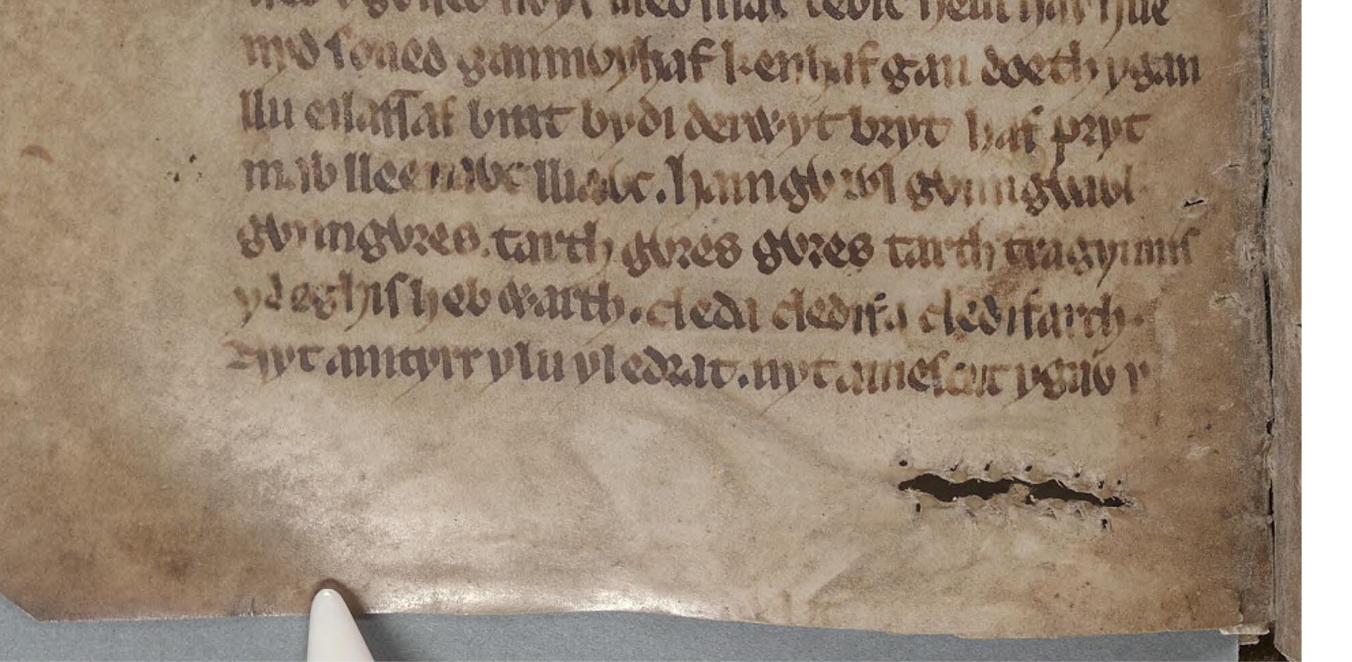
\includegraphics[width=\textwidth]{3orth/images/canvas.png}
%     \caption[The bottom of \acrshort{bt} p.~64]{The bottom of \gls{bt} p.~64. Image credit: The National Library of Wales}
%     \label{fig:p64}
% \end{figure}
The easiest way to account for this situation is that scribe X86  copied the word \mw{kywlat} twice. First, he wrote it as a catchword to make sure the quire starting with page 65 would be placed immediately following the quire ending with page 64. Second, it  is the first word of page 65. In the first instance, he adds orthographic representation of lenition and in the second he copies his exemplar directly. The reason he did not add lenition in the second instance is most likely because he forgot about the syntactic context of this word by the time he had his next quire before him. This instance singularly tells us that scribe X86 was the one who added orthographic lenition to his texts, and that his exemplar did not represent lenition in writing.


\subsection{Sims-Williams}
\label{sec:sims-williams}

\Textcite[107n]{Sim_Buchedd18} writes in his edition of \mw[]{Buchedd Beuno} that `[s]ometimes the radical is written even when lenition is required grammatically, \eg \mw[his patrimony]{y \al{t}reftat ef}; \mw[from exhaustion]{o \al{t}rablinder}; \mw[from this kingdom]{o'r \al{t}eyrnnas honn}'. Here he notices the bare fact that lenition is sometimes not written, and although all his examples start with \mw[]{t},  he does not state that non-lenition may be conditioned by the initial consonant. I found that lenition is not represented twelve times in \mw[]{Buchedd Beuno}, and every single one of these instances starts with \mw[]{t}. This implies that there was a period or an area where lenition of \mw[]{p, c} was written but not \mw[]{t}\footnote{Although I cannot confirm the existence of such a phase in Chapter~\ref{cha:indep-comp-mwbr}, manuscripts \gls{sB}\gls{sE} in Chapter~\ref{cha:welsh-laws} do show noticeably more non-lenition of \mw[]{t} than of \mw[]{p}. In this case, the pattern is muddied by the fact that these manuscripts have complicated textual histories.}.

However, lenition of \mw[]{t} is represented more frequently than it is not. Another saint's life found in the same manuscript  is that of Saint David discussed in Chapter~\ref{cha:stemm-mwbuch-dewi} as \gls{j119}. Here, it is concluded that orthographical lenition of \mw[]{c} was found in the original Welsh composition because it is represented consistently, while lenited \mw[]{p, t} are represented inconsistently, and were therefore added to the text at a later stage. This makes it difficult to pinpoint the time or place when only lenited \mw[]{t} was not represented, because the life of Saint David in \gls{j119} is only a copy of a text which has this pattern, not the text itself. The same must be the case for \mw[]{Buchedd Beuno}.

\subsection{Van Sluis}
\label{sec:van-sluis}
Existential verb \oes\ and the verbal ending \ei\ are noticed by~\textcite{van_development14} as causing lenition to immediately following subjects and objects alike, but not to \mw[]{p, t, c}\footnote{Earlier work, such as \textcite[§~21]{evans_grammar_1964} and \textcite[§~70]{morgan_y_1952} already found that these verbal endings regularly cause lenition irrespectively of the syntactic function of the element lenited, but did not notice a restriction to particular consonants. This restriction was not noticed by \textcite[§~71]{morgan_y_1952} because he operated from the principle that unwritten lenition may always represent spoken lenition, but written lenition may never represent spoken non-lenition.}. This behaviour contrasts with other types of postverbal lenition, such as lenition of objects and predicates. This pattern is observed in some of the earliest Mabinogion texts, \ie \mow{Culhwch ac Olwen} and \mow{Pwyll Pendefig Dyfed}. These texts are found in the \gls{wbr}, which dates from the mid-fourteenth century, but are thought to have been composed earlier\footnote{\Textcite[43]{rodway_date_2005} dates the composition of \mow[]{Culhwch ac Olwen} to the second half of the twelfth century, but is unsure about \mow[]{Pwyll Pendefic Dyfed}~\autocite[59]{Rod_Where07}. The \gls{wbr} dates to the mid-fourteenth century~\autocite[59]{huws_medieval_2000}.}. The following examples  illustrate the system found in~\textcite{van_development14}:
\begin{mwl}
  \mwc{\acrshort{wbr}~2.2-4}%
  {ac ual ẏ llathrei \al{ỽ}ynnet ẏ cỽn ẏ llathrei \al{c}ochet ẏ clusteu}%
  {And as white as the dogs shone, so red shone their ears.}%
  \mwc{\acrshort{wbr}~481.22}%
  {canẏt oes \al{l}estẏr ẏn ẏ bẏt a dalhẏo ẏ llẏn cadarn hỽnnỽ namẏn hi.}%
  {Since there is no vessel in the world that may hold the strong drink except for this one.}%
  \mwc[storch]{\acrshort{wbr}~483.23}%
  {Nẏt oes \al{t}orch ẏn ẏ bẏt a dalhẏo ẏ gẏnllẏuan namẏn torch canastẏr kanllaỽ}%
  {There is no collar in the world that may hold the leash except for the collar of Canastr Canllaw.}%
\end{mwl}
Because non-lenition of \mw{p, t, c} is found following postverbal contact lenition, but not following object lenition or lenition of the predicate, \textcite{van_development14} considers this non-lenition a specific feature of \ei\ and \oes\ only; however in light of the difference in orthography between \gls{bbc} and \gls{h}, it may make more sense to think of non-lenition of \mw[]{p, t, c} following \ei\ and \oes\ as an older orthographical stratum, and to think of lenition of the object and nominal predicate as later innovations in the text\footnote{In fact, \textcite{van_development14} describes how object and predicate lenition gained ground in the \gls{mw} period. Chapter~\ref{cha:welsh-laws} explores how older orthographical strata may be transmitted in later \gls{mw}.}.

\section{Stop orthography as a dating criterion}
\label{sec:lenit-voic-stops-1}
Students of Welsh quickly learn to recognise the difference between \gls{ow} (9th--11th centuries), \gls{mw} (12th--14th centuries) and \gls{mow} (15th century onwards) based on where lenition is represented. \Gls{ow} has no orthographic lenition even though we know it existed in the spoken language, while \gls{mw} does have orthographic lenition, except for \mw{d, rh}. \Gls{mow} has orthographic lenition for all consonants that lenite phonologically, including \mow[]{d, rh}. Thus, a student can easily identify just on the basis of where lenition is represented whether any text before him dates from the \gls{ow} period, the \gls{mw} period, or the \gls{mow} period.

I propose one more intermediate stage between \gls{ow} and \gls{mow}: in early \gls{mw}, lenition of voiceless stops was not represented orthographically word-initially, while in later \gls{mw} it was. Thus, early \gls{mw} texts may be recognised as such because they do not represent lenition of voiceless stops, and late \gls{mw} texts may be recognised as such because they do. This proposal raises the question as to when these lenited voiceless stops came to be represented with \mw[]{b, d, g}. In a text where  lenition is represented orthographically, except for voiceless stops, we may postulate a \lat{terminus ante quem} as well as a \lat{terminus post quem} for its original composition: it must originally have been composed before lenition of voiceless stops was represented orthographically, and after lenition started being represented at all.

One goal of Part~\ref{part:orthography} is to pinpoint more precisely  the origin of orthographical lenition of voiceless stops, so as to more precisely date texts having or lacking this feature. Moreover, \textcite{van_development14} saw that some grammatical environments are particularly conservative in the sense that lack of orthographical lenition may carry over in newer texts. When these environments can be identified, then traces of  earlier orthographical strata in younger manuscripts may be found, which is another goal of Part~\ref{part:orthography}.

\section{Other dating criteria}
\label{sec:other-dating-crit}

It is helpful to compare this task with earlier efforts to date and localise \gls{mw} texts based on linguistic or orthographical criteria. An example of a datable development in Medieval Welsh is the relative frequency of third-person singular preterite indicative ending \mw[]{\mbox{-w(y)s}} and \mw[]{\mbox{-awdd}}. \Textcite{Rod_Datable98} sees a marked increase in the use of \mw[]{\mbox{-awdd}} in the work of thirteenth-century poets compared to their twelfth-century counterparts. Poetry from about 1300 has near-universal \mw[]{\mbox{-awdd}}. He also studied the relative frequency of these markers in prose, and they change in roughly the same period in prose as they did in poetry. \Textcite[68--71]{Rod_Two03} adds to this verbal ending the third-person singular imperfect endings \mw[]{\mbox{-i}} and \ei, the former of which gradually fell out of use during the twelfth and early thirteenth centuries. Still, there was no period in which \mw[]{-i} was more common than \ei. Another such variable is the shift from third-person singular present subjunctive \mw[]{\mbox{-wy/-oe}} towards \mw[]{-o}. \Textcite[71--73]{Rod_Two03} then observes a dramatic rise of \mw[]{\mbox{-o}} in the first half of the thirteenth century, although the situation in poetry is somewhat different from that in prose. The ending \mw[]{-o} was consistently employed as early as the twelfth-century \mow{Braint Teilo}, and \textcite[73]{Rod_Two03} finds only one occurrence of \mw[]{-wy} in prose in \mow[]{Culhwch ac Olwen}. \Textcite{Rod_Where07} provides an example of the way in which the relative incidence of verbal endings may help in creating a rough chronology, and how this methodology compares to other methods in establishing the date and location of medieval literature. The most complete overview of which verbal endings are typical of which period is given by \textcite[166]{rodway_dating_2013}, which shows that compounding insights into the chronology of several developments allows one to date texts with a precision of roughly half a century.

Many of the developments Rodway describes occurred in the thirteenth century and therefore they seem to be roughly contemporaneous with the shift towards representing lenition of voiceless stops. Also, Rodway notices how prose and poetry sometimes, but not always, differ in the extent to which they reflect language change, so textual genre may serve as a confounding variable\footnote{I have not found any consistently differing orthographies of lenition between poetry and prose. Changing the orthography of lenition differs from changing verbal endings in that changing the former is purely orthographical, while making changes in verbal endings changes poetry when it is spoken as well, and may cause rhyme or alliteration patterns to break.}.

%% PSW is not too relevant after all

\Textcite{Tho_Middle93} proposes that linguistic criteria may be used not only for dating the composition of a text, but also for geographic identification. Two of his variables are applicable to this discussion:  stem-formative yod, which may be present or absent, \eg \mw[sureties]{meychyeu/meicheu} as well as stem-formative \mw[]{-th-/-t-} in inflected forms of \mw[with]{gan} and \mw[between]{rwng}, \eg \mw[with him]{ganthaw/gantaw}\footnote{His third variable is third person singular \mw[]{-awd/-ws}, but \textcite{Rod_Datable98}  shows that variation here is chiefly chronological, not dialectal.}. Here, high incidence of yod is associated with north Wales, and low incidence with south Wales. For the inflected prepositions, stem-formative \mw[]{\mbox{-th-}} generally appears in north Wales, and \mw[]{\mbox{-t-}} appears in south Wales. Consequently, there is a strong positive correlation between these features: high frequency of yod implies high frequency of stem-formative \mw[]{\mbox{-th-}}. This research illustrates the value of considering multiple linguistic variables when establishing time and place of composition. If one wishes to establish the place of a text's composition, but the text is too short or lacking in sufficient tokens to judge its dialectal affiliation based on either variable, then one may use both variables to reach a reliable judgment.

The case of stem-formative yod is more complicated than described previously, however. \Textcite{Rus_Celtic90}, for example, notes that variation between \mw[]{\mbox{-awc}} and \mw[]{\mbox{-yawc}} is  lexically conditioned to a great extent, so that incidence of yod in a text does not correlate solely with its geographical origin; incidence of yod is also more frequent in some words or morphemes than other words or morphemes. \Textcite[106]{Wil_Lexical05}  additionally states  that some words show no variation at all, meaning that these items occur with or without yod in both north and south Welsh, and the items that do vary do so according to a pattern reminiscent of lexical diffusion of sound change\footnote{Lexical diffusion occurs when a modification is expressed in a subset of a language's lexicon only, and then spreads gradually to other lexical items.}. \Textcite[116]{Wil_Lexical05} then lists fourteen lexical items that occur frequently and show variability regarding presence or absence of yod in his corpus of northern and southern law manuscripts. He notes that the relative frequency of yod has the following order, from low  to high frequency of yod: \mw[relics]{kreir(y)eu} < \mw[pregnant]{beich(y)awc} < \mw[testimony]{tyst(y)olaeth} < \mw[lawful]{kyfreith(y)awl} < \mw[laws]{kyfreith(y)eu} < \mw[witnesses]{tyst(y)on} < \mw[already]{eiss(y)oes} < \mw[try]{keiss(y)aw} < \mw[bullock]{eid(y)on} = \mw[penny]{kein(y)awc} < \mw[sons]{meib(y)on} < \mw[priest]{effeir(y)at} < \mw[eye-witnesses]{gwybyd(y)eit} < \mw[men]{dyn(y)on}. This order means  that \mw[]{kreir(y)eu} appears with yod in relatively fewer instances and in fewer manuscripts than \mw{beich(y)awc} does, for example. \Textcite[117]{Wil_Lexical05} also finds that agreement exists between the texts about the nature of the variation, meaning that one may somewhat confidently predict that a text using yodless \mw[]{meibon} will also use yodless \mw[]{tyston}, because the former item has yod appearing more frequently than the latter. The raw percentages given by \textcite{Tho_Middle93} do not reflect this complexity.

Willis's methodology and observations demonstrate the importance of comparing  manuscript texts that are as similar to each other as possible, except for the variable under study. Chapter~\ref{cha:indep-comp-mwbr} provides a comparison of translations of the same text, and they chiefly differ in the date of their translation into \gls{mw}. Consequently, the different texts under consideration are similar in variables such as genre and vocabulary, but they represent diffent stages of the language. Willis's observations also teach us that the evidential value of a single form containing or not containing yod  differs from word to word. In \mw[]{kreir(y)eu}, for example, yod is quite rare across manuscripts, so a manuscript writing yod is strong evidence for a northern affiliation. Conversely, yodless \mw[]{kreireu} is a more trivial find, so it is not as strong an indicator of southern affiliation. The reverse is the case with \mw[]{effeir(y)at}, where yod is found in a high percentage of instances and a majority of manuscripts have yod; therefore, absence of yod in this word strongly indicates a southern affiliation, while presence of yod is rather trivial. Chapter~\ref{cha:stemm-mwbuch-dewi} discusses how manuscripts may share representation of lenition, or they may share a lack of representation. Both types of  instances may be used to argue for a close stemmatic relationship, but the evidential value of represented lenition or its absence depends on the grammatical environment that causes lenition, just as the evidential value of stem-formative yod in establishing dialectal affiliation depends on the word in question.

\section{Overview}
\label{sec:overview}

This section is an overview of the chapters in Part~\ref{part:orthography} and describes the ways they  cumulatively build understanding of the orthographical development of lenited voiceless stops.

Chapter~\ref{cha:some-phon-issu} primarily treats methodological issues. It establishes that a phonological contrast between \lT\ and \xD\ only existed word-initially and thus, only word-initially is there a development to be studied. Therefore, this thesis  only considers word-initial lenition, and not word-medial or word final lenition. This requires a working definition of `word', yet Chapter~\ref{cha:some-phon-issu} finds that a universal definition of `word' is not readily available, and it is perhaps theoretically impossible to define it across languages or across chronolects of a given language. Still, a working definition is reached for the purposes of this thesis. Because primary data in Part~\ref{part:orthography} comprises mostly the presence or absence of orthographical lenition in various \gls{mw} texts,  Chapter~\ref{cha:some-phon-issu} also gives a working definition of lenition. Finally, counting instances where lenition is not written implies exhaustive knowledge of rules governing \gls{mw} lenition. To accomplish this, I discuss the environments  found to cause lenition, and I discuss where non-orthographic lenition is held to exist even though it cannot be seen.

Chapter~\ref{cha:indep-comp-mwbr} establishes a chronology of the developments based on independent thirteenth- and fourteenth-century translations of Geoffrey of Monmouth's \lat{Historia Regum Brittanniae}, where three orthographical stages can be discerned. Up until the mid-thirteenth century, lenited \mw[]{p, t, c} were not represented; in the late thirteenth century, lenited \mw[]{c} was represented, but not \mw[]{p, t}; and in the fourteenth century, all three consonants had lenition represented. The snapshots of orthographical stages provided by these results can be used to date the original composition of hitherto undated texts.

Chapter~\ref{cha:welsh-laws} discusses the orthography of several law manuscripts that contain \mow[]{Llyfr Iorwerth}. Here, the goal is to chart ways that an original composition from before the  thirteenth century is changed as it is copied during the thirteenth century and onwards. The chapter finds that even the most innovative scribes from the fourteenth century preserve traces of older orthography, thus creating a textual form distinguishable from original compositions contemporary with these scribes. Moreover, the chapter explores  alternative ways in which scribes modernised lack of orthographic lenition beyond simply filling in lenition where there was an unlenited consonant previously. Finally, the chapter identifies indicators for comparing lenition in different manuscripts that may be used to argue for a particular stemmatic relationship, providing for the analysis in Chapter~\ref{cha:stemm-mwbuch-dewi}.

Chapter~\ref{cha:stemm-mwbuch-dewi} takes three manuscript witnesses of \mow[]{Buchedd Dewi}, and explores how correspondences or their lack in the orthography of lenition can be used to create a stemma of the various manuscript witnesses and even to allow for the dating of hypothesised nodes in this stemma. 


%%% Local Variables:
%%% mode: latex
%%% TeX-master: "../main"
%%% coding: utf-8
%%% End:

\chapter{The nature of words and lenition}
\label{cha:some-phon-issu}
I argue that a distinction between \lT\ and \xD\ was only maintained word-initially and only as a result of the morphophonological process of lenition. These two conditions, word-initialness and participation in grammatical lenition, may seem trivial to any educated speaker of Welsh, but speaker intuitions alone cannot  make sense of the patterns found in both the phonological and the orthographical part of my thesis. This chapter treats both issues.

\section{Word-initial contrasts and what a word is}
\label{sec:excl-word-init}
Part~\ref{part:phonology-phonetics} confirms that the phonological difference between \lT\ and \xD\ was only maintained word-initially. These consonant series must have merged word-medially and word-finally soon after \gls{apoc}, and possibly even before this development. Old Welsh evidence attesting to this merger is discussed in Section~\ref{bdgwithptc}. This finding is backed up by Cornish and Breton, where voiced geminates similarly merged with lenited voiceless stops, indicating that this merger most likely occurred as early as the Common Brittonic period~\autocite[31]{schrijver_old_2011}.

\section{The indeterminacy of word separation}
\label{sec:indet-word-separ}
Having established that \lT and \xD\ were only distinguished word-initially, the question arises as to the precise limits of this constraint, \ie it raises the question `what is a word?'.
To a non-linguist, this issue may seem trivial, but linguists have been unable to agree on a cross-linguistic definition of `word'.
\Textcite[28]{haspelmath_indeterminacy_2011} even argues that the whole search for a definition of the concept `word' is because we are biased by writing habits, and he remarks: 
% \tqt{Joseph Vendryes remarked that modern linguistics was in a crisis, and that linguists were not even in agreement on what a word is, one of the fundamental concepts of their object of studies.}{haspelmath_indeterminacy_2011}{28}
\tqt{Linguists have no good basis for identifying words across languages, and hence no good basis for a general distinction between syntax and morphology as parts of the language system.}{haspelmath_indeterminacy_2011}{24}
What this means is that any formulation of a morphological or syntactical rule may not use the term `word', because it is not a meaningful concept cross-linguistically, and it is not a meaningful concept within a language until it is defined explicitly. 
The history of Welsh in comparison with other Brittonnic languages already reveals inconsistencies in where speakers consider word boundaries  to exist.
A case in point is \gmow[by, against]{erbyn}, a single-word preposition in Welsh.
This word is reconstructed as \gpbr[before head/end]{ari penn\=u} \autocite[258]{schrijver_studies_1995}, a preposition followed by a noun.
This combination later grammaticalised into a compound preposition and finally into a simple preposition.
In \gls{mco} a trace of the original two-word syntax remains, as is borne out by infixed possessive pronouns in \mco[against you, him]{er-dhe-byn, er-y-byn}, \etc~\autocite[120]{koch_neo-brittonic_1989}.

Disambiguating word-internal consonant changes from word-initial mutations cross-linguistically is  a problem \textcite{iosad_right_2010} perceived in his overview of all languages with initial consonant mutations.
He refrains `from considering most cases of consonant alterations involving the left edges of units smaller than the word', as these alternations do not usually target first consonants specifically, and he notes that `the majority of these cases do not involve any morphosyntactic information'~\autocite[108]{iosad_right_2010}.
He then acknowledges immediately that his definition leaves some leeway and raises the question what it means to be initial in a word.
He then opts for `an intuitive notion of ``word'' as the actual instantiation of a lexical item, without committing to a particular stance'~\autocite[109]{iosad_right_2010}.
In the end, he gives two useful criteria for diagnosing a word-initial mutation: first, the morphophonemic process uniquely appears at the beginning of a word and second, it is used to convey morphosyntactic information.

This thesis argues that there were many instances where \lT
and \xD\ were kept apart, and also plenty of instances where they were not. 
So how do we formulate the limit of the applicability of this phonological distinction between the stop series?
Such a formulation must be borne out by the evidence. Based on orthographical evidence, \gls{mw} word segmentation agrees largely, but not completely, with where \gls{mow} orthography puts spaces between words.
Still, exceptions exist, \eg \gmow[together]{i gyd} is written as  one word in \gmw{ygyt}.

Crucially, morphemes and lexemes do not exist in isolation. 
Phonemes of the \lT -type only stand in phonemic contrast with \xD\ because a morpheme containing \lT\ coexists with one containing \xT, so the existence of a phrase such as \gmw[his father]{y dad} implies the existence of the lexeme \mw{tad}.
Conversely, the existence of \mw{tad} allows for the phonological interpretation of a phrase containing \lT\ to be maintained as such, so it is becaise of \mw{tad} that \mw{y dad} may be interpreted as /i \gls{l}tad/ rather than /i \gls{x}dad/.
A similar morphological relationship between phonemes may not be posited for word-medial and word-final consonants, \eg the existence of \gmw{tad} does not imply the existence of \gmw{**tat} or \mw{**tath}.
Thus, the link maintaining this phonological distinction between different variants of a lexeme does not exist word-medially and word-finally in the same way it does word-initially.

Compounds such as \mw{i gyd} `together' constitute a lexeme of their own, so that the existence of the word \mw[joining]{cyd} no longer influences the phonological structure of \mw{i gyd} in the same way that \mw{tad} influences \mw{ei dad}.  Thus, a speaker of \gls{mw} could no longer  interpret the phrase \mw{i gyd} as /i \gls{l}kɨd/ rather than /i \gls{x}gɨd/. Instead, a speaker of \gls{mw} would interpret the phrase as one word: /iˈgɨd/, and the opposition between \lT\ and \xD\ did not exist word-internally. In other words:  no mutation exists on a synchronic level, because the petrified mutation does not carry morphophonemic information.

\section{On lenition}
\label{sec:lenition}
To understand the contexts within which a difference between lenited voiceless stops and radical voiced stops may exist,
we must understand  the difference between a lenited and a radical consonant  in the first place. 
Again, this matter would seem obvious to educated speakers of Welsh, 
but I  argue that there are different types of lenition, 
and that not everything that looks like lenition behaves like it.

Lenition is the result of a sound law that occurred in the history of Brittonic when a lenitable consonant was found after a vowel and before either a vowel or a sonorant~\autocite[96]{mccone_towards_1996}. 
As long as these vowels and sonorants remained, these lenited sounds were predictable based on their phonological environment, \ie they were allophones of their radical counterpart. 
However, following \gls{apoc} --- the loss of final syllables --- this environment no longer existed, and the radical or lenited pronunciation of a consonant was no longer automatically conditioned by its phonological context, so the distinction between radical and lenited consonant became phonemic.

\subsection{Morphophonemic lenition}
\label{sec:morph-lenit}
Typically,  lenition operating in \gls{mw} creates a variant inflection of a single lexeme; for example, \gmow[father]{tad} is a lexeme with a form  inflected for lenition: \mow{dad}. 
Substituting one form for another has consequences for the morphosyntax of a phrase and may either change its meaning or make it ungrammatical.
In other words: lenition itself is grammaticalised, as the lenited and unlenited variant morphemes stand in non-free variation. Whenever this is the case, lenition may be considered morphophonemic.
This type of lenition is the primary research topic of this thesis. An overview of grammatical environments that cause \gls{morphophonlen} is found in Appendix~\ref{cha:envir-that-cause}.
Morphophonemic lenition may be subdivided into two categories: contact lenition and free lenition.
\subsubsection{Contact lenition}
\label{sec:contact-lenition}
Contact lenition occurs when lenition is applied to a word because it is a property of the immediately preceding word that it causes lenition; for example when lenition follows various prepositions or pronouns. 
When a preposition or pronoun causing contact lenition is used, failure to lenite the following word may either change the meaning of a phrase or make it ungrammatical, \eg failing to lenite \mow{ferch} in \mow[his daughter]{ei ferch} would change the meaning to `her daughter', and failing to lenite following the definite article in \mow[the daughter]{y ferch} would make the phrase ungrammatical, because  gender concord between the article and the noun would be lost.

Contact lenition is by far the most common type of lenition in \gls{mw}. Virtually all instances of contact lenition are a direct consequence of \gls{apoc} and the ensuing phonemicization of phonetic lenition. Contact lenition started out as a functionless morphophonemic property of a morpheme,  but this morpheme could acquire function if it contrasted with a homophone causing a different mutation~\autocite[1]{schrijver_free_2010}. This is exactly what we see with the different meanings of \mow[his, her]{ei}, where the pronouns themselves are homophonous, but \mow[]{ei} causes lenition when it means `his', but spirantisation when it means `her'.

\subsubsection{Free lenition}
\label{sec:free-lenition}
Free lenition is any type of lenition `where neither synchronic contact with a preceding morpheme nor former phonetic context can account for its occurrence'~\autocite[1]{schrijver_free_2010}. Unlike contact lenition, free lenition always has a function, and free lenition is not a direct result of \gls{apoc}. Because free lenition is not a direct result of \gls{apoc}, instances of free lenition may not automatically emended where it is expected, but not represented.

An overview of different types of free lenition is given by \textcite{schrijver_free_2010}. An example is lenition of a noun in apposition to another element in the phrase, \eg Example~\ref{pryderiuab}.
\mwcc[pryderiuab]{\gls{wbr} 36.17}{prẏderi	\al{uab} pỽẏll}{Pryderi, son of Pwyll}
Other examples are lenition of the object after the verb and lenition of nouns following a preposed adjective.
\Textcite{schrijver_free_2010} frames most instances of free lenition  as `lenition of apposition', where he employs a wide definition of apposition: `if two sememes have the same referent, the second is an apposition of the first'~\autocite[3]{schrijver_free_2010}, and where he gives the following rule for most instances of \gls{mw} free lenition: `If two sememes that belong to the same clause have the same referent, one, usually the second, is lenited'~\autocite[3]{schrijver_free_2010}.

\subsection{Petrification}
\label{sec:petrification}
Some \gls{mw} words may be lenited as a property of these words themselves rather than as a result of its syntactic role or the word immediately preceding it.
The lenited form in such cases may be the only form left within a speaker's grammar.
Alternately, a radical and a lenited form can exist side by side, but be interchangeable in any phrase. In such a case, lenition no longer serves as a morpheme, and wherever a lenited and unlenited form stand side by side, they stand in free variation, \eg \mw[over]{dros, tros}.

The resulting words are sometimes  arguably lenited in a diachronic sense, but never in a synchronic sense, because words where lenition is petrified do not alternate with unlenited counterparts under the morphophonemic conditions otherwise governing lenition. Petrified lenited forms may emerge as the result of two distinct processes: clitic reduction and reanalysis of morphophonemic reduction.

\subsubsection{Clitic reduction}
\label{sec:clitic-reduction}
Clitic reduction is the reduction of the phonological load of an unstressed word%
\footnote{Conjugated and bare forms of \mw[with]{can} exemplify how stress influences whether a word is reduced: stressed conjugated forms of this preposition still write their radical initial later than unstressed simple forms. Later lenition of conjugated variants may be due to analogy with the simple form~\autocite[54]{jongeleen_lenition_2016}.}. 
The voicing, fricativisation, or deletion of a consonant are some ways by which a word's phonological load may be reduced.
The result of such processes may look superficially identical to lenition.
A clitic may then become petrified in its reduced form when it becomes the unmarked or only form possible. 

This type of reduction is similar to free lenition in that it is not the result of the phonemicisation of phonetic lenition that occurred with \gls{apoc}.
However, this type of lenition differs from both contact lenition and free lenition in that the radical and the mutated form stand in free variation.
That is, one may use \mow[with]{gan, can} interchangeably without causing any change in morphology, syntax or semantics. 
Therefore, substitution of the radical for the reduced form or vice versa never makes a grammatical phrase ungrammatical~\autocite[451--453]{morgan_y_1952}. 

Over time, the reduced form may become the unmarked form or even the only form left. 
Such a reduced form may then itself become subject to clitic reduction. 
An example of this is the \gls{mw} preposition \mw[to]{y}. 
This word is the reduced form of \mw{dy} /ðɨ/, itself a reduced form of \gls{ow} \mw{di} /dɨ/\footnote{Cf.\ \gmob[to]{da}.}. 
\todo{Refer to JTK's GOW paragraph on irregular development of vowels in clitics when it is finished}
The development of \mw[to]{y} demonstrates that this clitic reduction does not necessarily follow established sound laws. 
There is no general pattern of /d/ turning into /ð/ in Welsh outside of the environment of lenition, and there is certainly no established pattern of /ð/ disappearinɡ completely.

Irish clitics witnessed a similar development.  
\goi[to]{co} and \goi[over]{tar} were pronounced with initial /g/ and /d/, despite being voiceless etymologically%
\footnote{
  An \gls{oir} sound law has been formulated for this voicing: `a voiceless dental stop or fricative on the word boundary was regularly voiced in contact with an unstressed vowel, but otherwise remained unvoiced'~\autocite[42]{mccone_final_1981}. 
  \Textcite[43]{jongeleen_lenition_2016} proposes a similar process for velars.
}.
\Gls{oir} lenition of /c/ and /t/ would give /θ/ and /x/, proving that lenition did not cause clitic reduction.
As a result, lenited \goi{**cho, thar} are not found, even though their conjugated counterparts and, therefore, stressed counterparts do show variation between lenited and unlenited variants~\autocite[43]{jongeleen_lenition_2016}.

\Textcite[16--17]{schrijver_studies_1995} discusses a potentially relevant phonological development.
Within the debate of where the stress historically fell in \gls{pbr},  \textcite{thurneysen_zur_1883} argues that there was a period in \gls{pbr} when the stress fell on the word-initial syllable.
This argument is based on comparison of the pretonic particle \gpc{*tu} in the noun \gmw[lord]{ty-wyssawc}, and in the verb \gmow[I say]{dy-weddaf}.
These two words show that a homophonous particle was weakened when it served as an unstressed preverbal particle, but was not weakened in nouns.
\Textcite{thurneysen_zur_1883} argues (and \textcite{schrijver_studies_1995} agrees) that \gls{pbr} had stress on the first syllable and that any particles preceding this syllable had their consonants  reduced from \pc{*t} to \mw{d}.
The question on which syllable stress fell is irrelevant at present, but the outcome of this discussion implies a  sound law where initial voiceless stops were voiced whenever they were unstressed.
This implied sound law has little in common with intervocalic lenition, but is more reminiscent of the type of reduction seen from \mw{can} to \mw{gan}, although the precise sound law operating here is never discussed independently of the British accent.
I suggest that the reduction of \pc{*tu} to \mw{dy} in \mw{dy-weddaf} may in fact be considered a form of clitic reduction and that this development was distinct from lenition\footnote{%
  \Textcite[125]{schrijver_studies_1995} also implies elsewhere that he considers clitic reduction a form of lenition: `However, the fact that the preposition always occurs in the lenited form, viz.\ Co.\ \textit{war}, MW \textit{ar} < \textit{*war} rather suggests that it was unstressed. […] Since, as we have seen, the preposition was always lenited[…].'}.

Clitic reduction can hardly be called a `sound law' in the Neogrammarian sense of the word, because such a sound law would must take into account that reduced and unreduced forms of the same word  exist side by side, \eg \gmow{tros, dros}\footnote{%
  Except, of course, if we considered the stressed and unstressed proto-forms of \mow{tros, dros} unrelated lexemes.
}.
The existence of such doublets is better paralleled by English contracted forms existing together with their fully expanded form, \eg \emph{do not, don't}.


Comparative evidence thus demonstrates that it is a misnomer to refer to clitic reduction as lenition.
Diachronically, the processes developed differently for the phonemicisation of lenition with \gls{apoc}, and the reduction of clitics: the former did so according to sound laws while the latter did so haphazardly.
Synchronically, petrified clitic reduction and lenition also bear little relation to one another. Lenition is a morphophonological process, meaning the difference between a radical and a lenited form is non-trivial, while a reduced clitic stands in free variation with its non-reduced counterpart, when the radical counterpart exists at all. 
These considerations show that clitic reduction is a qualitatively different process from morphophonemic lenition. 

\subsubsection{Reanalysis of morphophonemic lenition}
\label{sec:rean-morph-lenit}
In some cases,  a word is lenited so frequently that the word is reanalysed and the lenited consonant comes to be reconsidered as the radical.
% An example of this development is found in several \gls{mow} dialects in frequent words such as \mow[bridge]{pont}. 
% This feminine word is lenited to \mow[the bridge]{y bont} following the article. 
% This syntax may become petrified, and speakers may again lenite the resulting word to \mow[the bridge]{y font}.
Free lenition is frequently petrified, \eg in words typically or only used as adverbs: \mow[yesterday]{ddoe}, \mow[before]{gynt}. In \gls{mow} the unlenited forms of these words are virtually unknown.



In the first page of the Black Book of Chirk (\gls{sA}), an instance of this type of petrification is found: \mw{garauuys} and \mw[Lent]{ga/rauuys} in ll.~9, 9--10, respectively. 
Etymologically, \mw{grawys} is a feminine word, which comes from \glat{quadragēsima}, and both instances follow the article. 
It differs from morphophonemic lenition in that the latter type of lenition is not represented for \mw{c} in this text. 
Moreover, no attested instances of unpetrified exist *\mw{c(a)rawys} in Welsh, and it is reanalysed as a masculine noun~\autocite[s.v.~\mow{Grawys, Garawys}]{bevan_geiriadur_2014}. 

\Textcite[448-451]{morgan_y_1952} lists a few examples of petrified lenition. One of these is \mow[much]{fawr}, which provides another case study of reanalysed morphophonemic lenition. This word is often lenited in contexts where it denotes the degree of a negative: \eg \mow[where they did not receive much earth]{lle ni chawsant \al{fawr} ddaiar}, or following \oes: \mow[in whom there is not much consolation]{nad oes \al{fawr} gyssur ynddo}. Contexts like these have caused \mow[]{fawr} to be reanalysed as meaning `not much', and now the lenited form may be used even where there is no grammatical reason to expect lenition, \eg \mow[without understanding much of the lives of angels]{heb ddeall \al{fawr} o fywyd angelion} or \mow[that I do not now mention him much]{nad wyf i yr awron yn \al{fawr} sôn am dano}. Other examples include \mow[poor]{druan} in \mow[]{Dafydd druan} and \mow[I presume]{debygaf} in \mow[more, I presume, than in any other place in the world]{mwy, \al{dybygaf} i, nac yn lle arall o'r byt}.

Diachronically, petrification of morphophonemic lenition differs from petrification of clitic reduction. 
In the former case, we are dealing with the result of reanalysis of lenition, while in the latter case we are dealing with the petrification of a shift toward a form with lesser phonological load. 
Synchronically, however, both types of petrification are similar in that in neither case the radical and the mutated form stand in morphophonemic contrast to each other. 

\subsubsection{Behaviour of reanalysed lenition and clitic reduction}
\label{sec:their-behaviour}
Both types of petrification behave similarly to each other and differently from morphophonemic lenition. 
In both cases, \gls{D} descending from \gls{T} behaves like \xD\ rather than \lT. Phonological evidence from the cynghanedd implies that petrified voiced stops descending from voiceless stops alliterate with \xD\ rather than \lT\footnote{See Example~\ref{kymrawtdreic}.}.

Orthographical evidence shows that lenited voiceless stops were represented with \mw{b, d, g} from an earlier date onwards when lenition was petrified than when lenition was still morphophonemic. 
In other words: a text within regularly represented \gls{morphophonlen} of voiceless stops may still write clitic reduction and reanalysed lenition with \mw{b, d, g}. 
An example of a manuscript showing such a pattern is \gls{ll1}, which consistently writes \mw[together]{y gyt}, with \mw{g-}, because it is petrified as a close compound of \mw[to + union]{i + cyd}, even though this manuscript barely represents morphophonemic lenition of words with \mw{c-} as their initial consonant.

\Textcite[52]{jongeleen_lenition_2016} notes that conjugated prepositions of \mw{tros, trwy} are found with initial \mw{t-}  in thirteenth-century manuscripts, while later manuscripts employ spellings with \mw{d-}.
\Textcite{sims-williams_variation_2013} differentiates variant spellings of \mw[with me, with you]{kennyf, kennyt}, which may be spelled with initial \mw{k-/c-}, or with \mw{g-}.
He similarly notes that `\textit{k-/c-} seems to indicate a pre-fourteenth century date whereas \textit{g-} is neutral, being found at all periods of Middle Welsh'~\autocite[24]{sims-williams_variation_2013}. \Textcite[55]{jongeleen_lenition_2016} gives a relative chronology of these petrifications, noting that `[t]he simple preposition \textit{can} is the first to transition to its lenited form \textit{gan}, followed by \textit{tros} and finally \textit{trwy}'.

My editorial policy is to include petrified lenition and where lenition occurs within compounds like \mw{i gyd}, but to mark them as research exceptions; however, I do not do this with personal pronouns such as \mw{mi/ỽi}\footnote{The reason for this is that I only understood that expressions such sa \mw[]{i gyd} had to be marked research exceptions after seeing how they behaved. With personal pronouns, it is more obvious that their lenition is non-grammatical.}.

\section{Spirantisation and non-word-initial mergers}
\label{sec:spirantization}

Comparing and contrasting lenition with spirantisation offers some insight into the difficulties in establishing word boundaries, and  spirantisation was arguably only triggered non-word-initially.
Spirantisation is similar to the first merger of \lT\ and \xD\ in this regard, and its mechanics are, therefore, of interest to this thesis.
The fact that \gls{mow} still has spirantisation as a morphophonemic mutation is because the identification of word boundaries at the time of its phonemicisation differed from where word boundaries are placed in \gls{mow} orthography.

As noted in Section~\ref{sec:indet-word-separ}, it is impossible to consistently identify word boundaries across languages.
This also means that word boundaries may not be consistent within different stages of a single language.
The consequence of this point is that one may not give different rules for word-internal spirantisation and for word-external spirantisation without also defining a `word'.
An overview of phonetic contexts in which spirantisation occurred is given by \textcite[2--3]{schrijver_spirantization_1999}, and he separately lists external sandhi causing spirantisation and internal sandhi.
These lists largely overlap.
Word-external sandhi is the most problematic diachronically, because this is where we see the greatest differences between Welsh and Breton.

Table~\ref{tab:envscausingspir} gives an overview of  environments that cause spirantisation in \gls{mw}.
None of the environments causing spirantisation in this table  constitute an open word class \ie nouns, verbs, or adverbs. In \gls{mob}, Spirantisation occurs in a few additional environments, but these environments are either similarly closed word classes, \eg \mob[va]{my}, \mob[their]{o}, or they are fixed expressions denoting a place-name or a single concept, \eg place-name \mob[]{Poher} < \glat{pagus} + \mob{kaer} and \mob[Easter Sunday]{Sul Fask} < \mob{Pask}.
These place-names  and fixed expressions may be considered a single word for morphosyntactic purposes, \cf Section~\ref{sec:petrification}.
Spirantisation is quite unlike lenition in this respect, considering how lenition may occur, \eg following a feminine noun, or in a compound of two nouns. None of the environments mentioned in Table~\ref{tab:envscausingspir} (except perhaps the numerals \mw[3]{tri} and \mw[6]{chwech}) may truly be considered words in the sense that they may be used as an independent phrase, and all environments occur in closed word classes.
These elements are also typically unstressed, and may therefore be considered an affix to a stressed word.

\begin{table}[h]
  \centering
  \begin{tabular}{ll}
    \toprule
    \tch{Word class} & \tch{Instances} \\
    \midrule
    possessive pronoun & \mw[her]{y}, and its infixed variant \mw[her]{'w} \\
    numeral &  \mw[3]{tri}, \mw[6]{chwech} \\
    preposition & \mw[with]{a}; \mw[over, very]{tra} \\
    conjunction & \mw[and]{a}, \mw[if]{o},  \mw{no}, \mw[neither, nor]{na} \\
    \multirow{3}[0]{*}{preverbal particle} & negative particles \mw{ny, na},   \\
                     & affirmative particle \mw{neu, ry}, \\
                     & verbal prefixe \mw{go-, di-, dy-}, \etc \\
    interrogative pronoun & \mw[where?]{cw} \\
    \bottomrule
  \end{tabular}%
  \caption[Causes of spirantisation in \gls{mw}]{Causes of spirantisation in \gls{mw}~\autocite[§~24]{evans_grammar_1964}.}
  \label{tab:envscausingspir}%
\end{table}%


A separate approach of internal and external spirantisation is therefore better abandonded. An alternative view is given by \textcite[126--129]{koch_neo-brittonic_1989}, who does note that `a word boundary is not a phonetic concept'.
He then appeals to prosody: two stressed words which became one single stressed word, such as place name \mw{Mathafarn}, may show spirantisation.
Spirantisation also occurs with two semantic words, but with only one word accent, \eg \mw[her house]{y ˈthy}.

The fact that we nowadays write a space between conjunctions, articles, and adverbs, \etc and the following word is not grounded linguistically, meaning such a space does not indicate a fixed level of morphosyntactic distance between the elements separated by it. Consequently, the conventions for writing spaces may differ between other languages, \eg \glat[and men]{virum-que}, Danish \textit{stol-en} `the chair'.
Moreover, verbal prefixes in words such as \mw[take care]{go-chel} are not considered separate words, even in Welsh.
If  these elements causing spirantisation may not be considered independent words, then spirantisation may not be considered a process involving two separate words.
Rather, it may be considered a specific type of internal sandhi where a word takes one of these prefixes.

Most pre-\gls{apoc} masculine  nouns and adjectives ended in an \pbr{*s}.
We know \gpbr{*s} caused spirantisation within a prosodic unit, \eg \gpbr{esjās tatos} > \gmow[her father]{ei thad}, yet masculine nouns followed by another prosodic unit never cause spirantisation.
This lack of spirantisation after nouns and adjectives is easily explained when we consider these elements independent words for the purpose of spirantisation.
Considering that they are typically stressed and make sense as independent phrases, the difference between nouns and adjectives on the one hand, and the environments causing spirantisation on the other hand, lack of spirantisation in the former group can hardly be a coincidence.

These considerations show that the phonological development of spirantisation has a lot in common with the merger of \xD and \lT: both occurred at non-phrase initial position, and the combined result of this merger and spirantisation entailed the loss of phonemic length in stops non-word-initially.
A final point of similarity is that both innovations occurred during the \gls{pbr} period, after the the Brittonic-Goidelic split (Goidelic has neither development), but before the split of \gls{pbr} into Welsh, Cornish, and Breton.

\section{Definitions for lenition and words}
% Perhaps we may turn the question of word segmentation around, and we may answer the question `what is a word?' on the basis of where \lT\ and \xD\ were kept apart. 

Both the problems of word segmentation and lenition --- seemingly very different problems --- lead to the same key in answering their respective issues: 
\begin{itemize}
\item `Morphophonemic lenition' in \gls{mw} is where both \gls{x}\gls{C}  and \gls{l}\gls{C} are possible initial phonemes of a given morpheme and where  substitution of either variant phoneme for the other has consequences for the grammaticality or the semantics of a phrase.
\item A `word' in \gls{mw} is any lexeme which has both \gls{x}\gls{C} and \gls{l}\gls{C} as possible initial phonemes for variant morphemes and where  substitution of one variant phoneme for another has consequences for a phrase's grammaticality or semantics.
\end{itemize}
This definition of `word' is not a satisfying definition beyond the scope of this thesis, because a strict reading  invalidates any lexeme starting with \mw{s, h, ch, n} or a vowel as a word, because these sounds may not be lenited. It is, however, satisfying as a criterion for determining the mutations included in the databases  given in Appendix~\ref{cha:database-lenition} and Appendix~\ref{cha:datab-lenit-mwbuch}.


%%% Local Variables:
%%% mode: latex
%%% TeX-master: "../main"
%%% End:

\chapter{Independent compositions of \mw{Brut y Brenhinedd}}
\label{cha:indep-comp-mwbr}
This chapter analyses the orthography of lenition in the Welsh translations of the  \lat{Historia Regum Brittanniae} by Geoffrey of Monmouth, a Latin-language historical prose text dating from the twelfth century.
Translations of this text into Welsh date from the thirteenth century onwards.
In total, there are some sixty manuscripts containing some sort of translation or rendition of this history, and they may be divided into six individual classes.
Each of these classes contains independent translations of the Latin text; some of them may be considered faithful translations, whereas others handle the source material more freely~\autocite[xxiv-xxxi]{roberts_brut_1971}.

The existence of several independent translations or reworkings of a single text made over much of the \gls{mw} period is valuable in studying linguistic or orthographical developments.
These texts are valuable because their manuscript witnesses are roughly contemporaneous with the composition of their translation.
Additionally, the independence of these translations means that each version makes for a reliable snapshot of the language and orthography of its time and place.
At the same time, the fact that all the \gls{mw} texts are translations of the same text in Latin offers a controlled research environment:  any difference in the language of the translations cannot be due to differing subject matter.
As such, differences in the Welsh translations are controlled for the variable of subject matter.
The importance of comparing texts containing similar lexical content is shown by \textcite{Wil_Lexical05}, who shows that language change in \gls{mw} may occur at different times for different words.
Comparing different translations of the same text ensures that a lexical item occurring frequently in one translation should occur similarly frequently in another.
Similarly, we know that the translations of are all translations from Latin, meaning the variable of source language is also controlled for.
Geoffrey of Monmouth's Latin is generally straightforward, and his vocabulary and grammar do not generally give any trouble~\autocite[lxxvi]{Geo_History09}.
The independence of these translations and the concurring independence of orthographies contrasts with the law texts discussed in Chapter~\ref{cha:welsh-laws}, as those law texts tend to be Welsh-language copies of Welsh-language texts, carrying over some old orthography.
The fact that we deal with translations of a Latin text means that any occasions where lenition may give rise to ambiguities may be resolved by comparing the Welsh to the Latin.
However, medieval translations are not necessarily faithful to the original:
\tqt{\begin{welsh}
  Nid yw'r cyfieithwyr hyn, fwy na chyfieithwyr cyffredin y cyfnod canol, yn gaeth i'r testun Lladin. […] Newidir rhai manylion neu ychwanegu rhai brawddegau er mwyn cysylltu'r hanes â ffynonellau eraill.%
\end{welsh}%
\footnote{These translators are not slavish to the Latin text any more than typical translators of the medieval  period. […]
  Some details are changed, or some sentences are added in order to connect the history with other sources.}}{Rob_Testunau74}{290}
Nevertheless, the subject matter of each text --- no matter how many details are altered --- remains historiography, so wildly differing rates of lenition found in each translation cannot possibly be caused by differing subject matter found in each manuscript.

Caution is needed when dealing with translations if the language of the original Latin seeps through into the grammar of the Welsh.
The result of this is that some constructions are more frequent than would be expected in a Welsh prose text:
\tqt{
  \begin{welsh}
    Gadawodd y Lladin ei hôl ar arddull y cyfieithiadau, yn yr ansoddeiriau lluosog, a'u safle o
flaen yr enw, yng nghytundeb berf â'i goddrych, yn y gystrawen berthynol, yn y defnydd o enwau
haniaethol, ac o ansoddeiriau berfol i gyfleu rhangymeriad gorffennol, yn y trosi llythrennol o
elfennau gair cyfansawdd, yn y cystrawennau trwsgl a'r colli gafael ar rediad brawddeg wrth geisio
llunio brawddegau cymhleth yn hytrach na brawddegau cydradd, byrion y testunau brodorol.%
  \end{welsh}%
\footnote{The Latin left its mark on the form of the translations, in the plural adjectives, and their place before the noun, in the agreement of the verb with its subject, in the relative clause, in the use of abstract nouns, and of verbal adjectives to convey past participles, in literally translating elements of compound words, in the clumsy sentences and in losing the grip on the flow of a sentence from trying to fashion complex sentences instead of the coordinate, short sentences of the original texts.}
}{Rob_Testunau74}{289}
The most important point here is the placement of adjectives before the noun they qualify.
Wherever this happens, the element following the preposed adjective is lenited.
The use of these adjectives is possible in Welsh, but is highly stylized%
\footnote{Adjectives that always come before the noun they modify, \eg \mw[old]{hen}, are not highly stylized in this position.}.
Because translating from Latin brings preposed adjectives out more frequently in Welsh they may have been misunderstood occasionally, as they caused some erratic behaviour, as found in Example~\ref{ex:wychyrcalet}.
There is also a more obvious feature showing these texts were translated from Latin: Latin personal names are found and code switching to Latin also occurs.  

All in all, their syntax shows these translations tend to be slavish on the sentence level compared to present-day translations, but freely deviate from the Latin original in terms of content. 





\section{Versions used}
I have taken four different manuscript witnesses of \mw{Brut y Brenhinedd} from four classes for analysis.
Three of these are thirteenth-century manuscripts, and the fourth is from the fourteenth century.
\Textcite{Rob_Testunau74}  notes that these three translations  are similar in terms of how well they are translated.  
\tqt{
  \begin{welsh}
    Fe'i  cyfieithwyd [yr \textit{Historia}] deirgwaith yn  y drydedd ganrif ar ddeg, ac ymddengys fod dau o'r fersiynau hyn, sef hwnnw sydd yn Peniarth 44, a'r un sydd yn Llansteffan 1, yn perthyn i flynyddoedd cynnar y ganrif.
    Dichon fod y trydydd, fersiwn Brut Dingestow, ychydig yn ddiweddarach.
    Y mae iaith y tri fersiwn yn debyg, a chyffelyb hefyd yw safonau'r cyfieithwyr a'u hagwedd at y testun Lladin.%
  \end{welsh}%
\footnote{The [Historia] was translated three times in the thirteenth century, and it appears that two of these versions, \ie the one that is in Peniarth 44, and the one that is in Llansteffan 1, belong to the early years of the century. It seems that the third, the  Brut Dingestow version, is a bit more recent. The language of the three versions is similar, and the standards of the translators and their attitude towards the Latin texts are also similar.}
}{Rob_Testunau74}{288--289}
\Textcite[xxix]{roberts_brut_1971} notes that all three translations are `close renderings of the Latin', and that all translations are independent.
This makes all of these three  manuscripts good independent snapshots of thirteenth-century orthography.
However, when the methods of translation between these three versions are compared, some differences may be identified \autocite{Rob_Testunau74}.
While the \gls{ll1} translation is the most faithful one of the three in both style and contents, the \gls{p44} translation is faithful tothe Latin on the level of the individual sentence, but leaves out some parts, and the translation found in \gls{bd} is the freest in terms of style as the text is shortened by summarising rather than selecting parts of the original:
\tqt{
    \begin{welsh}
Er mor debyg yw ymateb y tri chyfieithydd i'r Historia, y mae eu dull o gyfieithu'n amrywio. Gŵr
cydwybodol, gofalus oedd cyfieithydd fersiwn Llansteffan 1. Ychydig iawn a hepgorodd o'r testun
Lladin ond ceisiodd ei drosi frawddeg wrth frawddeg, hyd yn oed yn y manylion. Ef, yn sicr, a
luniodd y cyfieithiad mwyaf ffyddlon, er bod ei arddull braidd yn drwsgl. Yr oedd ei
destun Lladin ef hefyd yn wahanol mewn mannau i'r un a ddefnyddiwyd gan y ddau gyfieithydd
arall. Diddordeb cyfieithydd Peniarth 44 oedd rhediad yr hanes ei hun. Y mae ganddo arddull
weddol naturiol, uniongyrchol ac adroddiadol. Gall fywiogi'r hanes ond ei nodwedd gyffredin yw ei
fod yn ei gwtogi fel yr â rhagddo, trwy dorri allan frawddegau ac adrannau cyfain, nes y ceir ganddo,
erbyn y diwedd, grynodeb go chwyrn o'r Lladin. Llwyddodd cyfieithydd Brut Dingestow yntau i
gwtogi'r hanes, ond ceisiodd ef dalfyrru'n fwy deallus, nid trwy dorri adrannau allan, ond trwy
grynhoi wrth gyfieithu, a thrwy aralleirio, gan gadw'r cyfan o'r hanes, a hynny mewn Cymraeg digon
llyfn at ei gilydd, gydag adleisiau o'r arddull draddodiadol.%
\end{welsh}%
\footnote{However similar the response of the three translators is to the Historia, their method of translation varies. The translator of Llansteffan 1 was a conscientious, careful man. He left out very little of the Latin text, and tried to translate it sentence by sentence, even down to the details. He, surely, composed the most faithful translation, although his style is quite awkward. His Latin text was also different  from the one used by the other two translators in some places. The translator of Peniarth 44 was interested in the flow of the history itself. He has a fairly natural, direct, and narrative style. He may enliven the history, but his general trait is to abbreviate what comes before him, by cutting out whole sentences and parts, so that he gives in the end quite a drastic summary of the Latin. The translator of Brut Dingestow managed to abbreviate the history, but he tried to condense in a more intelligent way, not by cutting out sections, but by summarizing while translating, and by rewording, while keeping the whole of the history, and this in  fairly smooth Welsh on the whole, with echoes of the traditional style.}
}{Rob_Testunau74}{292--293}
These differences notwithstanding, considerable Latin influence is found in all three versions.
An example of this may be found in Examples~\ref{ll1llyr}, \ref{p44llyr}, and \ref{bdllyr}, where each translation has \mw[two daughters]{dwy ỽerchet} with a plural noun following the numeral, following Latin rather than Welsh grammar.

One of the earliest manuscripts containing the \mw{Brut} is \gls{ll1}, which
is dated mid-thirteenth century\todo{ref from Huws}.  A part of
the manuscript contains another version, namely a fragment
of \gls{p44}. The scribe was not a translator, as may be judged from
some mistakes and omissions~\autocite[xxxvii]{roberts_brut_1971}. This manuscript is shown by \textcite[80--81]{Rod_Datable98} to have comparatively high incidence of preterite ending \mw[]{-awdd} compared to \mw[]{-wys} for its period. 
I used lenition on pages 33 to 38 for analysis.



The \gls{p44} translation of the \mw{Brut} is roughly as old as the \gls{ll1} one, although \textcite[85]{Rus_Orthography93} argues on orthographic grounds that it is written before \gls{ll1}. The manuscript is written by the same hand as \gls{sC}, discussed in Chapter~\ref{cha:welsh-laws}.
\Textcite[xix]{Lew_Brut42} states that \gls{p44} and \gls{ll1} are based on a common original translation, undoubtedly because the \gls{ll1} manuscript contains a fragment of the \gls{p44} translation, but according to \textcite[xliii--xliv]{Rob_Astudiaeth69}  they are based on separate translations.
I analysed lenition on pages 23 to 28.

\Gls{bd} is found in the following manuscript: \gls{nlw} MS 5266.
It is dated to the end of the thirteenth century~\autocite[xliii]{Rob_Astudiaeth69}.
An edition of this text is prepared by \textcite{Lew_Brut42}.
His introduction does not mention the orthography of lenition.
I analysed lenition found on pages 26 to 36.




\Gls{bcc} is the latest manuscript under consideration.
It contains the only translation from after the thirteenth century among the texts analysed in this chapter.
It dates from the mid-fourteenth century according to~\textcite[xlv]{Rob_Astudiaeth69}, and from the second quarter of the same century according to \textcite[xviii]{Jon_Brenhinedd71}.
\todo{The scribe of this \mw{Brut y Brenhinedd} translation is identified as scribe X89. (relevant?)}
I took lenition on folios 16r to 19v for analysis.

\Textcite{Rob_Testunau74} notes that the \gls{bcc} translation departs from the original in more ways than just summarizing, as it also incorporates other sources of history:
\tqt{
  \begin{welsh}
Cyfieithiad newydd yw Cotton Cleopatra lle y mae'r gwaith o gymathu â ffynonellau
eraill yn llawer mwy amlwg. Y mae'n fyrrach na'r Historia gan fod y cyfieithydd wedi torri'r areithiau
a llawer o'r disgrifiadau o'r brwydrau, ac wedi hepgor llawer o'r manylion. Ond o'r tu arall, y mae
yma lawer o ychwanegu sy'n gwneud y fersiwn hwn yn fwy storïol na'r un arall.%
\end{welsh}%
\footnote{Cotton Cleopatra is a new translation, where the incorporation of other sources is much more obvious. It is shorter than the Historia because the translator cut out the speeches and many of the descriptions of the battles, after removing many of the details. But on the other hand, there are many additions that make this version more storylike than any other one.}
}{Rob_Testunau74}{293}


\section{Method}
\label{sec:method}
From each manuscript, I have collected instances of orthographical
lenition as well as instances of where orthographical lenition would
be expected, but is not found. The sample used comprises roughly the
story of Llŷr and his daughters.  Some 250 data points are taken
from each manuscript.

\Gls{petr}, both the type resulting from grammatical lenition and from clitic reduction have been collected for prepositions
and (historically) nouns, but not for personal pronouns such
as \mw[I]{mi/fi}. The reason why these forms are included --- albeit
as research exceptions --- is that their orthography also changed over the
thirteenth century\footnote{See \ref{sec:petrification}.}. Including them allows
us to gauge when this happened relatively to \gls{morphophonlen}.
Including them also allows us to understand how easy it is to miss how \gls{morphophonlen} of voiceless stops was barely ever represented in the earliest translations, because \gls{petr} was already common in the same period.

It is not always clear what types of lenition applied in different
stages of \gls{mw}. Particularly some types of \gls{freelen},
such as object lenition and \gls{np} lenition tend to be used only irregularly,
or only in later texts~\autocite{van_development14}, but
with no distinction for consonant type. Evidence for the existence of
lenition differs between texts here, precluding a catch-all policy for
the inclusion of such instances. I generally look for multiple positive
instances attesting to the lenition of objects and \gls{np}s.
Consequently, I do not consider non-lenition of \mw[dead]{marỽ} in
Example~\ref{ex:bvmarw} to be relevant for the orthography of lenition,
because \gls{np} lenition is only found once elsewhere in this corpus.
As it happens, it is found in the same sentence.
This implies that \gls{np} lenition was grammatically optional.
\mwcc[ex:bvmarw]{\gls{ll1} 38.9--10}
{en e tryded wlwydyn gwedy henny e \al{bỽ ỽarỽ} llyr.\ ac e \al{bỽ marỽ} aganyppỽs brenyn ffreync}{In the third year after that Llŷr \al{died}, and Aganippus, king of France, \al{died}.}


\section{An overview of the results}
\label{sec:comparison-versions}
Let us look at one sentence found in all the manuscripts in a similar form.
This sentence demonstrates how the orthography of lenition developed in the thirteenth and fourteenth centuries.
\begin{mwl}
  \mwc[ll1llyr]{\acrshort{ll1} 34.16--18}{Ac ena hep ỽn gohyr
    o \al{k}yghor y \al{w}yrda ef ar rodes e dwy \al{ỽ}erchet hynaf
    ydaỽ yr deỽ \al{t}ewyssaỽc. nyt amgen tewyssaỽc kernyw ac ỽn
    gogled}{And then without any delay of counsel of his noblemen, he
    gave his two eldest daughters to the two princes, none other than the
    prince of Cornwall and the one of [the] North.}
  \mwc[p44llyr]{\acrshort{p44} 24.21--23}{Ac ena ny \al{b}ỽ ỽn gohyr
    o \al{k}yghor y \al{w}yrda er rodes ef e dwy \al{ỽ}erchet hynaf y
    deỽ \al{t}ewyssaỽc nyt amgen a thewyssaỽc kernyw. a thewyssaỽc e
    gogled.}{And then there was no delay of counsel of his noblemen
    that he gave his two eldest daughters to two princes, none other than
    the prince of Cornwall and the prince of the North.}
  \mwc[bdllyr]{\acrshort{bd} 31.6--7}{A hep \al{o}hir
    o \al{g}yt\al{g}yghor y \al{w}yrda y rodes ef y dỽy \al{u}erched
    hynhaf ydaỽ y \al{t}ywyssogyon yr alban.\ a chernyỽ. }{And without
    delay of counsel of his noblemen, he gave his two eldest daughters
    to the princes of Scotland and Cornwall.}
  \mwc[bccllyr]{\acrshort{bcc} 17r.21--24}{Ac yna yn diohir y rodes ef
    y dwy \al{v}erchet hynaf y deu \al{d}ywyssawc nyt amgen tywyssawc
    kernyw ar hwnn yr alban}{And then without delay he gave his two
    eldest daughters to two princes, none other than the prince of
    Cornwall and the one of Scotland.}
\end{mwl}
Roughly speaking, Examples~\ref{ll1llyr} and \ref{p44llyr} from the mid-thirteenth century show that lenited voiceless stops were not written.
Example~\ref{bdllyr} from the late thirteenth century shows lenition of \mw{g}, but not of \mw{t}, and thus forms an intermediate stage before voiceless stops were all written lenited.
The final stage of full lenition is found in Example~\ref{bccllyr}.
Table~\ref{tab:perlenbrut} confirms these impressions: only a minority of lenited \mw{p, t} is written until \gls{bcc}, while a minority of lenited \mw{c} is only written until \gls{bd}%
\footnote{This result shows that the behaviour of Scribe X86 is not unique to this scribe. See Section~\ref{sec:haycock}.}.


\begin{table}[h]
  \centering
  \begin{tabular}{lddddddd}
    \toprule
    \tch{Manuscript} & \tch{\mw{b}} & \tch{\mw{g}} & \tch{\mw{ll}} & \tch{\mw{m}} & \tch{\mw{p}} & \tch{\mw{t}} & \tch{\mw{c}} \\
    \midrule
    \acrshort{ll1} & 82.1 & 72.1 & 83.3 & 98.2 & 0.0 & 9.1 & 35.8 \\
    \acrshort{p44} & 82.5 & 36.1 & 78.6 & 91.7 & 8.3 & 13.3 & 29.1 \\
    \acrshort{bd} & 89.7 & 98.4 & 87.5 & 100.0 & 22.2 & 33.3 & 92.2 \\
    \acrshort{bcc} & 67.9 & 98.5 & 85.7 & 100.0 & 95.8 & 83.3 & 86.2 \\
    \bottomrule
  \end{tabular}%
  \caption{Lenition including research exceptions represented in the \mw{Brut}, in percentages.}
  \label{tab:perlenbrut}
\end{table}

\begin{table}[h]
  \centering
  \begin{tabular}{lddddddd}
    \toprule
    \tch{Manuscript} & \tch{\mw{b}} & \tch{\mw{g}} & \tch{\mw{ll}} & \tch{\mw{m}} & \tch{\mw{p}} & \tch{\mw{t}} & \tch{\mw{c}} \\
    \midrule
\acrshort{ll1} & 82.1 & 72.1 & 83.3 & 98.1 & 0.0 & 0.0 & 8.7 \\
\acrshort{p44} & 82.5 & 36.1 & 78.6 & 91.4 & 8.3 & 0.0 & 7.3 \\
\acrshort{bd} & 89.7 & 98.4 & 87.5 & 100.0 & 22.2 & 0.0 & 88.0 \\
\acrshort{bcc} & 67.9 & 98.5 & 85.7 & 100.0 & 95.8 & 80.0 & 78.6 \\
    \bottomrule
  \end{tabular}%
  \caption{Lenition excluding research exceptions represented in the \mw{Brut}, in percentages.}
  \label{tab:perlenbrutex}
\end{table}

Table~\ref{tab:perlenbrut} gives the raw numbers of how much lenition we see where we would expect it, which includes instances of \gls{petr} such as \mw[together]{y gyt} (\gls{p44} 25.11).
Table~\ref{tab:perlenbrutex} excludes these research exceptions, leaving us with only \gls{morphophonlen}.
Comparison between Table~\ref{tab:perlenbrut} and Table~\ref{tab:perlenbrutex} shows that most early instances of lenited \mw{c} written with \mw{g} are in fact instances of \gls{petr}.
The contrast between these percentages shows how easy it is to miss out on how  \gls{morphophonlen} was written only for a few consonants, when \gls{petr} is there to block this view.

\section{Lenition of voiceless stops}
\label{sec:lenit-voic-stops}

Table~\ref{tab:perlenbrutex} shows how rarely morphophonemic lenition of \mw{p, t, c} is represented in the earlier translations of the \mw{Brut}. The orthographical development of these consonants will be discussed in this section.

\begin{figure}[h]
  \centering
  \begin{tikzpicture}
    \begin{axis}[
      width=.9\linewidth,
      height=.6\linewidth,
      xlabel=Manuscript,
      ylabel={Representation of lenition (\%)},
      symbolic x coords={
        \gls{ll1},
        \gls{p44},
        \gls{bd},
        \gls{bcc}
      },
      xtick=data,
      legend style={legend pos=north west},
      ]
      \addplot[color=black,rounded corners,thick,dotted,] coordinates {
        (\gls{ll1},0.00)
        (\gls{p44},8.33)
        (\gls{bd},22.22)
        (\gls{bcc},95.83)
      };
      \addplot[color=black,rounded corners,thick,dashed,] coordinates {
        (\gls{ll1},0.00)
        (\gls{p44},0.00)
        (\gls{bd},0.00)
        (\gls{bcc},80.00)
      };
      \addplot[color=black,rounded corners,thick] coordinates {
        (\gls{ll1},8.70)
        (\gls{p44},7.32)
        (\gls{bd},88.00)
        (\gls{bcc},78.57)
      };
      \legend{\mw[]{p},\mw[]{t},\mw[]{c}}
    \end{axis}
  \end{tikzpicture}
  \caption{Orthographical representation of voiceless stops over time.}
  \label{fig:linechartbrut}
\end{figure}

\subsection{Lenition in \acrshort{ll1} and \acrshort{p44}}
\label{sec:lenit-acrsh-acrsh}


The rule is clear in \gls{ll1} and \gls{p44}: lenition of voiceless stops is not written.
Given this rule, exceptions, constituting instances of representation of lenited voiceless stops, need to be accounted for.
These exceptions are found in Table~\ref{tab:ltrepll1p44}.
As can be seen in this table, both the form and meaning of the words themselves and their reason for being lenited differs, so accounting for them must be done on a case-by-case basis, and a satisfying account may not always be found.

\begin{table}[h]
  \centering
  \begin{tabular}{lddwql}
    \toprule
    \tch{Source} & \tch{Page} & \tch{Line} & \tch{Word} & \tch{Translation} & \tch{Reason lenition} \\
    \midrule
    \acrshort{ll1} & 34 & 1 & gellweyr & jest & \mw{trwy} \\
    \acrshort{ll1} & 35 & 8 & gytdỽundep & agreement & \mw{o} \\
    \acrshort{ll1} & 36 & 4 & gof & memory & \mw{ar} \\
    \acrshort{ll1} & 37 & 17 & glaf & sick & \mw{en} \\
    \acrshort{p44} & 25 & 10 & gewylyd & shame & \mw{en} \\
    \acrshort{p44} & 26 & 2 & gynt & before & adv phrase \\
    \acrshort{p44} & 26 & 9 & bryt & moment & \mw{pa} \\
    \acrshort{p44} & 27 & 6 & glaf & sick & \mw{en} \\
    \bottomrule
  \end{tabular}%
  \caption{Instances of \lT\ represented in \acrshort{ll1} and \acrshort{p44}.}
  \label{tab:ltrepll1p44}
\end{table}

One word that may be accounted for, however, is \mw[before]{gynt} (\gls{p44} 26.2).
It stands out in that it is the only lenited adverbial phrase in this source.
Moreover, lenition of adverbial phrases of time is often petrified, \eg \gmow[yesterday]{ddoe}.
The writing of \mw{gynt} with \mw{g} may similarly point to \gls{petr}, rather than \gls{morphophonlen}.
If so, this word constitutes a research exception.

The case of \mw[what moment?]{pa bryt} may be explained in a similar manner.
Although lenition following \mw{pa} is morphophonemic and still grammatical, it occurs frequently in combination with \mw{bryt}, so orthographical lenition is reminiscent of the \gls{petr} we find in research exception \mw[together]{y gyt}.
Comparison with phrases  such as \gmob[when]{peur < pe eur} also shows that interrogative pronouns containing \mw{pa} may be considered single words for the purpose of lenition.
Also, the semantics of the phrase obviously have a temporal dimension similar to \mw{gynt}.
The phrase \mw{pa bryt} is also found with exceptional lenition in \gls{bd}, as can be seen in Table~\ref{tab:replenpbd}.

After accounting for these two examples, we are still left with six examples of orthographically represented \gls{morphophonlen}.
These examples are few and far between, but nevertheless essential, because they show that lenition of voiceless stops \emph{could} be represented.
This means that writing \graph{b, d, g} for \lT\ had already been invented by the mid-thirteenth century.
It had just not been adopted widely.


\subsection{Lenition in \acrshort{bd} }
\label{sec:lenition-acrshortbd-}
In \gls{bd}, the rule is that lenition is not represented for \mw{p, t}, and it is represented for \mw{c}.
This rule is exceptionless for \mw{t}, but not for \mw{p} and \mw{c}.
These exceptions constitute instances where lenition is represented for \mw{p}, and for \mw{c} these exceptions constitute instances where lenition is not represented.
Table~\ref{tab:replenpbd} shows the two instances of orthographically represented lenited \mw{p}, and Table~\ref{tab:nonlencbd} shows every instance where lenited \mw{c} is not orthographically represented.

\begin{table}[h]
  \centering
  \begin{tabular}{addwql}
    \toprule
    \tch{Source} & \tch{Page} & \tch{Line} & \tch{Word} & \tch{Translation} & \tch{Reason lenition} \\
    \midrule
    bd & 34 & 4 & bryt & moment & \mw{pa} \\
    bd & 36 & 2 & baraỽt & ready & \mw{yn} \\
    \bottomrule
  \end{tabular}
  \caption{Representation of lenited \mw{p} in \acrshort{bd}}
  \label{tab:replenpbd}
\end{table}

\begin{table}[h]
  \centering
  \begin{tabular}{addwql}
    \toprule
    \tch{Source} & \tch{Page} & \tch{Line} & \tch{Word} & \tch{Translation} & \tch{Reason lenition} \\
    \midrule
    bd & 29 & 10 & caerussalem & (place name) & fem noun \\
    bd & 30 & 14 & kyuoeth & kingdom & \mw{y} ‘his' \\
    bd & 31 & 8 & kyuoeth & kingdom & \mw{y} ‘his' \\
    bd & 31 & 9 & kyuoeth & kingdom & \mw{y} ‘his' \\
    bd & 33 & 2 & caffei & received & \mw{na} \\
    bd & 35 & 1 & keissyaỽ & seek & \mw{y} ‘to' \\
    \bottomrule
  \end{tabular}%
  \caption{Non-representation of lenited \mw{c} in \acrshort{bd}}
  \label{tab:nonlencbd}
\end{table}

\subsection{Lenition in \acrshort{bcc}}
\label{sec:lenition-acrshortbcc}


Lenition of voiceless stops is as a rule represented in \gls{bcc}, so instances where lenition is not shown are the ones that need to be accounted for.
Table~\ref{tab:ltnotrepbcc} shows these instances of non-represented lenition.
Various reasons for lenition appear multiple times in this table.



\begin{table}[h]
  \centering
  \begin{tabular}{lddwql}
    \toprule
    \tch{Source} & \tch{Page} & \tch{Line} & \tch{Word} & \tch{Translation} & \tch{Reason lenition} \\
    \midrule
    \gls{bcc} & 16r & 29 & prosessio & procession & \mw{y} ‘to' \\
    \gls{bcc} & 16v & 6 & keluydodeu & arts & prep adj \\
    \gls{bcc} & 17r & 14 & kereis & I loved & \mw{th} \\
    \gls{bcc} & 17r & 15 & caraf & I love & \mw{th} \\
    \gls{bcc} & 17r & 16 & kerir & is loved & \mw{th} \\
    \gls{bcc} & 17v & 18 & tywyssauc & prince & apposition \\
    \gls{bcc} & 17v & 29 & tywyssawc & prince & apposition \\
    \gls{bcc} & 18r & 12 & trugarhae & mercy & \mw{y} ‘his' \\
    \gls{bcc} & 18r & 25 & Cordeilla & (personal name) & \mw{-ei} \\
    \gls{bcc} & 19r & 10 & Cordeilla & (personal name) & \mw{-ei} \\
    \gls{bcc} & 19v & 4 & tywyssawc & prince & apposition \\
    \gls{bcc} & 19v & 4 & tywyssawc & prince & apposition \\
    \gls{bcc} & 19v & 5 & calet & hard & prep adj \\
    \gls{bcc} & 19v & 13 & cordeilla & (personal name) & \mw{y} ‘to' \\
    \gls{bcc} & 19v & 25 & creftwyr & craftsmen & prep adj \\
    \bottomrule
  \end{tabular}%
  \caption{Instances of \lT\ not represented in \acrshort{bcc}.}
  \label{tab:ltnotrepbcc}
\end{table}

Within \gls{bcc}, \mw[prince]{tywyssawc} is found four times in apposition to a personal name.
A lenitable noun in apposition to a personal name is found eight times within this source, and is lenited only once in \mw[prophet]{broffwid} (\gls{bcc} 16r.26).
Lenition of nouns in apposition is not shown for other types of consonants either, as the word \mw[king]{brenhin} is also found in unlenited form in this position.

The word \mw{prosessio} is a late, learned loanword from \glat[procession]{prōcessiō}.
Writing \glat{c} in this word with \mw{s} confirms a post-vernacular pronunciation.
Phonologically, the structure of the word does not look Middle Welsh, as /au/ had not yet turned into /o/ in the final syllable.
This means that \mw{prosessio} constitutes an instance of code switching, or a recent loan.
Recent and transparent loanwords are not typically mutated in \gls{mow}, nor are instances of code switching.

The personal name \mw{Cordeilla} is found unlenited where lenition is expected on three separate occasions.
The fact that we are dealing with a personal name here may be of influence, as \mw{llyr} is found unlenited following \mw[fort]{caer} twice.
Furthermore, personal names are as a rule not lenited in \gls{mow}.
These instances of \mw{llyr} and \mw{Cordeilla} may be early examples of this \gls{mow} rule.
Additionally, \mw{Cordeilla} is a foreign name for the Welsh, and it may thus not have been lenited similarly to \mw{prosessio}.

Infixed object pronoun \mw{'th} should cause lenition, but this is not found in \gls{bcc}.
Lenition is problematic diachronically, as this pronoun causes provection in \gls{mco} and \gls{mb}.
Arguably, provection following this pronoun is also found in \gow[as it brings you]{imalitiduch} where medial \ow{t} represents both the /θ/ of the object pronoun, and preverb \ow{di} > \ow{ti}.

Several words following a preposed adjective fail to show lenition, although these instances are outnumbered by preposed adjectives shown to cause lenition.
Lenition following preposed adjectives is a type of free lenition, because all adjectives cause lenition when used as a preposed adjective.
These same adjectives do not as a rule cause lenition when they are in their usual postnominal position.
Consequently, the correct application of lenition hinges on the morphosyntactic relationship between two elements in the same clause rather than by simply checking whether the immediately preceding morpheme should cause lenition.
This morphosyntactic relationship may not always be clear or consistent.
Preposed adjectives are more frequent in this text than in \gls{mw} in general, because it is a translation from Latin, which further increases the likelihood of inconsistencies in the application of preposed adjectives.
An example where lenition following a  preposed adjective is to be expected is Example~\ref{ex:wychyrcalet}:
\mwcc[ex:wychyrcalet]{\gls{bcc} 19v.3--6}{ac yn ev herbyn wynt y doeth Maglawn tywyssawc yr alban. a henwyn tywyssawc kernyw ac ev holl allu. ac ymlad yn \al{wychyr calet} ac wynt.}{And against them came Maglawn, prince of Scotland, and Henwyn, prince of Cornwall, and their whole capability, and they fought \al{violently hard} against them.}
What exactly is the grammatical relationship between \mw[violent]{wychyr} and \mw[hard]{caled}?
Is \mw{wychyr} a preposed adjective followed by lenition, and translating to the translation given, or does \mw{caled} modify \mw{wychyr}, and are we not to expect lenition here?
In the latter case, `very violently' would be a more suitable translation%
\footnote{The Latin original is of little help either, as it is much terser than the Welsh: \lat[When this was done, Leir took his daughter and the assembled army to Britain. He fought with his sons-in-law and beat them.]{Quo facto, duxit secum leir filiam et collectam multitudinem in Britanniam pugnauitque cum generis et triumpho potitus est.}~\autocite[42--43]{Geo_History09}}.
And does the meaning matter at all for lenition?
At any rate, non-lenition is consistent, as the \mw{Brut} found in \gls{bcc} has four different instances of \mw{wychyr calet}, and each of them keeps the radical: 19v.5, 25v.14, 47v.12, 51r.29.
\Textcite[31--32]{morgan_y_1952} argues that constructions of the type  \mw{yn} + adjective + adjective  may be considered dvandva compounds or as compounds where one adjective typically has an intensifying function.
In any case, the repetition of adjectives constitutes the creation of a compound adjective, and thus always cause lenition, but that southern dialects tend to keep the radical here.
If Morgan is right, the example of  \mw{wychyr calet} seems like an aberration in both cases, because the second element should be lenited irrespectively of its semantics.
In the end, non-lenition may be a purely southern dialectal feature.

Many exceptions to the representation of lenition in \gls{bcc} stem from the difficulties involved in translating a Latin text.
After accounting for these, lenition seems to have been applied with great regularity, and remaining exceptions seem no more numerous than what is found in a \gls{mow} text of similar length, barring only the most carefully copy-edited ones.
As such, \gls{bcc} demonstrates that lenition of voiceless stops was wholly represented by the mid-fourteenth century.

\section{Lenited \mw{g}}
\label{sec:lenited-mwg}
The only number in Table~\ref{tab:perlenbrut} or Table~\ref{tab:perlenbrutex} not referring to a voiceless stop and dipping below the fifty per cent mark is that of the representation of lenited \mw{g} in \gls{p44}.
This begs the question why \mw{g} in \gls{p44} --- and to a lesser
extent in \gls{ll1} --- is lenited so infrequently.  In \gls{ll1}
lenited \mw{g} is shown in 49 out of 68 instances; in \gls{p44} it
is written in  only 26 out of 72 instances.  The element causing lenition
does not seem to be relevant, \eg verbal particle \mw{a} regularly
causes lenition to \mw[did]{oruc}, but not to \mw[did]{gwnaeth}.

The phonology of the lenited word does seem to play a role: when
initial \mw{g} is not followed by \mw{w}, it disappears in 48 out of
52 of such instances. The remaining four comprise the following
instances: \mw[they rested]{gorffowyssassant} (\gls{ll1} 38.25),
\mw[rested]{gor/ffowyssỽs} (\gls{p44} 23.9--10), \mw[gain]{gorescyn}
(\gls{p44} 27.15), and \mw[glorious]{gogonedỽs} (\gls{p44}
28.23). These words all historically started with \mw{g\cw}, but  \mw{\cw}
preceding \mw{o} has disappeared by the end of the \gls{ow} period. However, such words
starting with \mw{go} do represent lenition elsewhere, such as in the
plentiful instances of \mw[did]{oruc}.

The remaining 88 instances are all words starting with \mw{(g)w}, of which 27 show lenition.
Table~\ref{tab:gwphon} shows that the phonological structure of these words plays an important role in dictating whether lenition is written.
If the \mw{w} following lenited \mw{g} is vocalic, lenition is usually shown.
An example of such a word showing lenition is \mw[husband]{wr} (\gls{ll1} 34.13).
Similarly, lenition is usually shown if the quality of the following \mw{\cw} is consonantal, if this consonant is in turn followed by a vowel, \eg \mw[wear]{wyscaỽ} (\gls{p44} 27.7).
However, if the \mw{g} is followed by consonantal \mw{\cw}, and then followed by yet another consonant, lenition is usually not written, \eg \mw[make]{gwneỽthỽr} (\gls{p44} 27.28).

\begin{table}[h]
  \centering
  \begin{tabular}{ldd}
    \toprule
    & \tch{\graph{w}} & \tch{\graph{gw}}\\
    \midrule
    /ɡ\cw{}\gls{C}/ & 3 & 48\\
    /ɡ\cw{}\gls{V}/ or /ɡu/ &24 &13\\
    \bottomrule
  \end{tabular}
  \caption{Lenition of \mw{gw} divided by phonological structure of the word.}
  \label{tab:gwphon}
\end{table}

Not representing lenited \mw{g} served a purpose: it served to distinguish consonantal \mw{w} from its syllabic counterpart if it followed \mw{g} and preceded a consonant.
Maintaining  radical \mw{g} in the face of lenition served to indicate that the following \mw{\cw} before another consonant was consonantal, so that no reader of a phrase like \mw[his wife]{ẏ gwreic} would ever be fooled into saying /i ur…/ before reading the rest of the phrase and having to correct himself to /i \cw raɪɡ/.

\section{Conclusion}
\label{sec:conclusion-brut}
Lenition of voiceless stops was generally not written in the early thirteenth century, but it was not unfamiliarity with the concept of using \graph{b, d, g} for historical \mw{p, t, c} that kept them from writing lenition as such.
After all, these letters were used for \gls{petr}, and in exceptional cases even for \gls{morphophonlen}.
In the late thirteenth century, lenited \mw{c} came to be written as \mw{g}, but a similar shift did not occur for \mw{p} and \mw{t}.
These  departures from the thirteenth-century norm give us one key insight: lenition could be represented by this period, it had just not become the norm yet.

The case of lenited \mw{g} shows how the question of whether and how to write lenition may interplay with seemingly unrelated conundrums. 
A scribe who wished to ensure that no consonantal \mw{\cw} was mistaken for a vocalic \mw{w} had to weigh this wish against his wish to write lenition.
The former wish took precedence for the scribes of \gls{ll1} and \gls{p44}, and their priorities make sense in an orthographical tradition where the writing of lenition was limited to only several consonants, and where ability to read out loud would have been held in high esteem.

So what was the conundrum for voiceless stops?
What wish had to be weighed against the wish to represent lenition of these consonants?
The obvious answer to this question is that \lT≠\xD.
If lenited voiceless stops had not yet merged with radical voiced stops word-initially, then confusing the two when speaking might have been just as embarassing as using a vocalic \mw{w} for a consonantal \mw{\cw}. 
According to this line of reasoning, the phonological distinction between \lT\ and \xD\ argued for in Part~\ref{part:phonology-phonetics} must have survived until the middle of the thirteenth century.

%\todo[inline,caption={gg}]{For General conclusion: this means that not showing \lT\ is evidence of a early composition; probably dating back to  the period when they had not yet merged with \xD. However, the \mw{Brut} also shows that not writing \xD\ = \lT\ was by {choice}, rather than {ability}. They were able to write \lT\ like \xD\ as early as the thirteenth century, but they had to weigh representation of lenition against  the correct pronunciation of \lT\ separate from \xD. Another scribe (\eg of the Book of Aneirin) may have had different priorities, and could represent lenition of \lT. Ergo, writing lenition of \lT\ is not by itself a marker of lateness, but not writing lenition of \lT\ is, by contrast, a marker of earliness.}
%%% Local Variables:
%%% coding: utf-8
%%% mode: latex
%%% TeX-master: "../main"
%%% End:

\chapter{The transmission of the Welsh laws}
\label{cha:welsh-laws}

In this chapter, I analyze where lenition was represented in the various law texts.
The laws have existed in a written form since at least the early thirteenth century, and continued to be copied throughout the remainder of the Middle Welsh period. Taken together, these facts mean that the law texts lend themselves to investigation into how scribes copied manuscripts and when they maintained or changed the non-representation of lenited voiceless stops.

Lenition of voiceless stops was represented orthographically by the mid-fourteenth century, so manuscripts from around this period are most useful to chart this change in orthography.
Earlier manuscripts serve to demonstrate that the law texts indeed saw a period in which lenition of voiceless stops was not represented, even though lenition of other consonants was.
Later manuscripts may still show traces of the early orthography, allowing me to identify specific environments within which non-representation of lenited voiceless stops may be preserved.
I focus on the transmission of \mw{Llyfr Iorwerth}, because most of the oldest law manuscripts contain this law text, while there are still some newer ones.
 
Wiliam notes the following about the extant manuscripts:
\tqt{{[N]}o MS.\ of those now extant can be regarded as the original Book of Iorwerth, for none of them is such that the others may reasonably be held to be derived from it. Nevertheless, it is probable that all of the Venedotian MSS.\ were copied directly or indirectly from a common archetype of the class, for there is too much similarity between them to allow a belief in their independent origin.}{wiliam_llyfr_1960}{xxi}
The fact that all extant manuscripts go back to one single written source well before orthographical lenition of voiceless stops means that we may safely assume that all instances of orthographically lenited voiceless stops found in these manuscripts are the result of scribal innovation arising from copying this text. 

% How are various manuscripts related to each other?
% It is nowadays thought that none of the earliest extant manuscripts is a direct ancestor of another extant copy.
% One author who did think this was J.\ Gwenogvryn Evans (Figure~\ref{fig:gwevanslli}).
% Rather, extant manuscripts are held to have common exemplars that no longer exist.
% Figure~\ref{fig:stemmatestb} gives a stemma for the Iorwerth manuscripts (and some more manuscripts), and I will use this stemma as a point of departure for my own research.

% Which manuscripts may be used for analysis?
% One useful manuscript is \textit{A}, the \gls{bbch}, dating from around 1250. This manuscript is one of the oldest law manuscripts, and its orthography is very unusual.
% Another useful manuscript is \textit{B}, which is also fairly old, and dates from the end of the thirteenth century.
% Other thirteenth-century manuscripts shown in Figure~\ref{fig:stemmatestb}: \textit{EC};
% early fourteenth century: \textit{G};
% other manuscripts in this stemma are all later than the fourteenth century.
% Some more useful manuscripts are: \textit{VW}, by scribe X86; \textit{Tr}, by Gwilym Was Da.

% What sections of the law texts are useful for analysis?
% Figure~\ref{fig:stemmatestb} shows that \textit{B} was  transmitted in part from several sources. This makes both the Test Book and the Laws of Country interesting targets for analysis, as the orthography of lenition may confirm or deny this peculiar reconstruction by Charles-Edwards.
% Figure~\ref{fig:stemmatestb} also shows that different parts of the Test Book may have been added in intermediate stages between Redaction I and the extant manuscripts.
% Comparison of these chunks with text found in all the manuscripts may prove useful in establishing at what point in time these chunks were added, and therefore when some of the hypothetical nodes in the stemma were written.

% \subsection{The law corpus}
% \label{sec:fleshed-out-research}
I will take a part of the tractate on suretyship for analysis.
This tractate is found in many manuscripts from the Iorwerth tradition, and those manuscripts vary in date from the mid-thirteenth century to 1404.
To be more specific, I will use \textcite[\S\S58--65]{wiliam_llyfr_1960} for analysis.

The tractate of suretyship is particularly suitable for analysis because it constitutes an archaic core of the Iorwerth law tradition, and may therefore safely be assumed to have had a textual form well before the dates of the first manuscripts --- the mid-thirteenth century\footnote{Compare, for instance \S101 on suretyship, on which \textcite[20]{stacey_archaic_1986} describes the Iorwerth version as preserving the most primitive version.}. We may consequently be fairly certain that lenition of voiceless stops was not represented orthographically in the latest shared ancestor of all extant manuscripts.

\section{On the manuscripts}
\label{sec:manuscripts}
I have taken eight manuscripts for analysis. I will discuss them here. I refer to these manuscripts using their manuscript sigla throughout the chapter\footnote{These manuscript sigla were coined by \textcite{owen_ancient_1841}.}\todo{Refer to Huws' repository when it is published.}.

The manuscript with the siglum \gls{sA} is  \gls{nlw}, Peniarth MS 29, also known as the Black Book of Chirk.
It is dated to the mid-thirteenth century and thought to have been produced in the Arfon region~\autocite[171]{Rus_Scribal95}.
Several scribes may be identified in the manuscript, but the material used here all comes from Hand D and a few lines by Hand E~\autocite[133--134]{Rus_Scribal95}.
Hand D's orthography is peculiar for the thirteenth century in that he writes /ə/ with \mw[]{a}, and he has many variant spellings for /θ/, such as \mw[]{s, h, sh, ht, sth}.
Hand E's work seems to be `the most regular and consistent of all scribes in [\gls{sA}]'~\autocite[152]{Rus_Scribal95}.
The irregular spelling of dental fricatives, along with some other orthographical irregularities, suggests that \gls{sA}'s exemplar was written in \gls{ow} orthography~\autocite[169]{Rus_Scribal95}. 

Manuscript \gls{sB} is also known as \gls{bl}, Cotton Titus D.~ii, and belongs to the late thirteenth century, and may have been produced in St Asaph~\autocite[v]{elias_golygiad_2007}. The orthography of \gls{sB} is more consistent than that of \gls{sA}. \Textcite[xlii]{wiliam_llyfr_1960} notes about the orthography that `[m]utations of initial consonants are sometimes indicated, sometimes not. The nasal mutation, however, is regularly shown'.

Manuscript \gls{sC} is known more fully as \gls{bl}, Cotton Caligula A.~iii, and may be dated to the mid-thirteenth century. Its scribe was the same scribe as the one of the \gls{ll1} and \gls{p44} manuscripts, both containing the \mw[]{Brut y Brenhinedd}. \Textcite[189]{huws_medieval_2000} argues that the manuscript was probably written in a monastic milieu in north-east Wales. He considers Valle Crucis in Denbighshire to be the most likely place of composition.

Manuscript \gls{sD} is also known as \gls{nlw} Peniarth MS 32, and as \mow[]{Y Llyfr Teg}. It was produced around 1404~\autocite[60]{huws_medieval_2000} in the Cwm Tawe area~\autocite[v]{elias_golygiad_2007}. The laws texts are all written by Scribe X91, who is described as writing with great regularity and legibility, and his orthography mostly conforms to what was expected of this period~\autocite{thomas_tei_2013}.

Manuscript \gls{sE} is more fully known as \gls{bl} Additional MS 14931. It was produced at the end of the thirteenth century, and is considered a sister manuscript to \gls{sA}. An addition was written near the end in the hand of \gls{sB}. These facts give a geographic connection either to Arfon or to St Asaph~\autocite[100]{charles-edwards_welsh_1989}.

Manuscript \gls{sG} is \gls{nlw} Peniarth MS 35. It is written in the early fourteenth century by a scribe identified by Daniel Huws as X87, in whose hand we also find a copy of the laws of the Cyfnerth group from South Wales~\autocite{smith_tei_2013}. It was probably produced in the Brycheiniog area~\autocite[v]{elias_golygiad_2007}. It is the first manuscript from the Iorwerth tradition with a southern provenance~\autocite{charles-edwards_introduction_1986}.

Manuscript \gls{sJ} is Oxford, Jesus College MS 57, and was written around 1400 by Hywel Vychan of Builth, who was also the principal scribe of the Red Book of Hergest~\autocite[100]{charles-edwards_welsh_1989}. The manuscript may be connected to the Cwm Tawe area~\autocite{james_llwyr_1993}.

Manuscript \gls{sK} is also known as \gls{nlw} Peniarth MS 40 or as \mw{Llyfr Calan}, and is written after 1469 by Lewis Glyn Cothi~\autocite{roberts_cyfraith_2011}. It contains four poems in the beginning addressed to the lord of Cefn Llys, suggesting that the manuscript was written in this area~\autocite[374]{evans_report_1899}.

The paragraphs selected for analysis correspond to the folio numbers, column numbers and line numbers in the manuscripts given in Table~\ref{tab:surety}. This text runs continuously in all of these manuscripts, except in \gls{sG}, where it is interspersed with other additions. Over 200 data points were taken from each manuscript for analysis, except for \gls{sJ}, which has shortened the tractate on suretyship considerably.  
\begin{table}[h]
  \centering
 \begin{tabular}{lddlld}
  \toprule
  MS            & Begin                   & End   & Date & Location                   & Data pts     \\ \midrule
  \gls{sA}            & 43.22                   & 48.11  & s.xiii\textsuperscript{med}             & Arfon  & 210         \\
  \gls{sB}            & 20r.22                  & 23v.17 & s.xiii\textsuperscript{2}      & St Asaph  & 234         \\
  \gls{sC}            & 155va.10                 & 161ra.7 & s.xiii\textsuperscript{med}              & Valle Crucis  & 229         \\
  \gls{sD}            & 52.19                   & 61.16  & ca.\ 1404         & Cwm Tawe  & 231         \\
  \gls{sE}            & 34.5                   & 39.13  & s.xiii\textsuperscript{2}     & Arfon/St Asaph   & 218         \\
  \multirow{2}{*}{\gls{sG}}   & 20r.1                   & 23v.11  & \multirow{2}{*}{s.xiv\textsuperscript{1}}& \multirow{2}{*}{Brycheiniog}  & \multirow{2}{*}{263} \\
                & 26r.1                   & 26v.12 &                     &  &           \\
   \gls{sJ} & 269.19 & 277.11 & ca.\ 1400 & Cwm Tawe & 147 \\
  \gls{sK}&68.19 & 77.23 & s.xv\textsuperscript{2}& Cefn Llys & 244 \\
  \bottomrule
 \end{tabular}
  \caption{The parts of each manuscript containing the relevant paragraphs of the tractate on suretyship in various recensions of \mw{Llyfr Iorwerth}.}
  \label{tab:surety}
\end{table}

\subsection{The geographical spread of the manuscripts}
\label{sec:geogr-spre-manuscr}

The places where the manuscripts are presumed to have been produced are given in Figure~\ref{fig:mslocs}. The geographic origin of a manuscript tends to be less certain than its date. This means that the locations on the map may be taken with a grain of salt. Still, it is reasonable that these localisations are not off by an order of magnitude, and that we may somewhat confidently classify the manuscripts geographically into two groups. The first group is found in North Wales, and comprises \gls{sA}\gls{sB}\gls{sC}\gls{sE}. All of these manuscripts may be dated to the thirteenth century. The second group is found in South Wales, and comprises \gls{sD}\gls{sG}\gls{sJ}\gls{sK}. These manuscripts are all from the fourteenth and fifteenth century.

\begin{figure}[h]
  \centering
  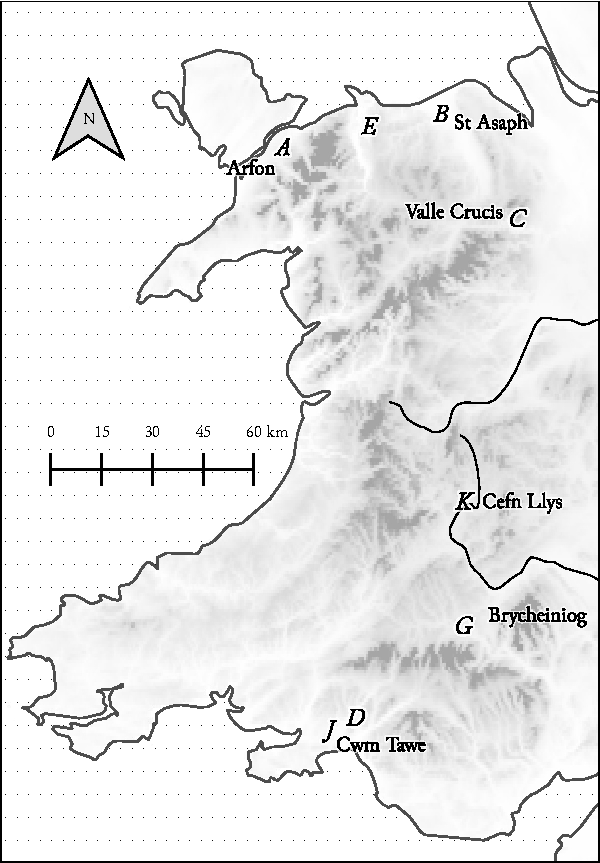
\includegraphics{3orth/images/mslocations.pdf}
  \caption[Locations of the law manuscripts.]{Locations of the law manuscripts analysed in this chapter. \gls{sE} is plausibly connected to both Arfon and St Asaph, so it stands halfway between them.}
  \label{fig:mslocs}
\end{figure}

Because the geographical split and temporal split occurs along the same lines, it is difficult to separate whether the different patterns of lenition found in these manuscripts are due to their temporal distance or due to their geographical distance.

\section{The stemmatic relationship of the manuscripts}
\label{sec:stemmata}
No manuscript named here has a surviving exemplar and all manuscripts share a common written ancestor. Despite the lack of surviving exemplars to the manuscripts discussed in this chapter, a rough stemmatic relationship between the manuscripts has been uncovered through text-critical methods. Figure~\ref{fig:twostemmata} shows two of the most recent insights into how they derive from a common ancestor, and which manuscripts may be considered to form independent subgroupings.

\begin{figure}[h]
  \newlength{\stemmalen}
  \setlength{\stemmalen}{2.5cm}
  \centering
  \begin{forest} for tree={font=\itshape,l=10mm,l sep=0mm,s sep=3mm,delay={where content={}{shape=coordinate}{}}}
    [X
    [α
    [γ
    [\gls{sA},l=20mm]
    [\gls{sE},l=25mm]
    ]
    [\gls{sC},l=30mm]
    ]
    [β
    [δ
    [\gls{sD},l=5.3cm,s=-6mm]]
    [ε
    [\gls{sG},l=35mm,s=-6mm]
    [ζ,s=6mm
    [\gls{sB},l=15mm]
    [\gls{sJ},l=4.3cm]
    [\gls{sK},l=5.5cm,s=6mm]
    ]
    ]
    ]
    ]
    \node at (forest cs:l=3cm,s=\stemmalen +.5cm) {1200};
    \node at (forest cs:l=5cm,s=\stemmalen +.5cm) {1300};
    \node at (forest cs:l=7cm,s=\stemmalen +.5cm) {1400};
    \node at (forest cs:l=9cm,s=\stemmalen +.5cm) {1500};
    \draw[dotted] (forest cs:l=3cm, s=-\stemmalen) -- (forest cs:l=3cm, s=\stemmalen);
    \draw[dotted] (forest cs:l=5cm, s=-\stemmalen) -- (forest cs:l=5cm, s=\stemmalen);
    \draw[dotted] (forest cs:l=7cm, s=-\stemmalen) -- (forest cs:l=7cm, s=\stemmalen);  
    \draw[dotted] (forest cs:l=9cm, s=-\stemmalen) -- (forest cs:l=9cm, s=\stemmalen);  
  \end{forest}
  \begin{forest} for tree={font=\itshape,l=10mm,l sep=0mm,s sep=3mm,delay={where content={}{shape=coordinate}{}}}
    [\textup{Redaction I}
    [α
    [\gls{sA},l=30mm]
    [\gls{sE},l=35mm]
    ]
    [\textup{Redaction II}
    [β
    [\gls{sC},l=20mm]
    ]
    [γ,
    [
    [\gls{sD},s=-6mm,l=4.3cm]
    [\gls{sG},l=25mm]]
    [
    [\gls{sB},s=0mm,l=15mm]
    [\gls{sJ},l=4.3cm,s=0mm]
    [\gls{sK},l=55mm,s=6mm]
    ]
    ]
    ]
    ]
    ]
    \node at (forest cs:l=3cm,s=\stemmalen +.5cm) {1200};
    \node at (forest cs:l=5cm,s=\stemmalen +.5cm) {1300};
    \node at (forest cs:l=7cm,s=\stemmalen +.5cm) {1400};
    \node at (forest cs:l=9cm,s=\stemmalen +.5cm) {1500};
    \draw[dotted] (forest cs:l=3cm, s=-\stemmalen) -- (forest cs:l=3cm, s=\stemmalen);
    \draw[dotted] (forest cs:l=5cm, s=-\stemmalen) -- (forest cs:l=5cm, s=\stemmalen);
    \draw[dotted] (forest cs:l=7cm, s=-\stemmalen) -- (forest cs:l=7cm, s=\stemmalen);  
    \draw[dotted] (forest cs:l=9cm, s=-\stemmalen) -- (forest cs:l=9cm, s=\stemmalen);  
  \end{forest}
  \caption[Two stemmata of the tractate on suretyship.]{Two stemmata of the tractate on suretyship, according to \textcite[138]{charles-edwards_iorwerth_1986} (left) and \textcite{charles-edwards_textual_2016} (right).}
  \label{fig:twostemmata}
\end{figure}

Both stemmata in Figure~\ref{fig:twostemmata} give a similar account of how the law manuscriopts are related. They differ in two aspects. Both stemmata show a particularly close relationship between \gls{sA}\gls{sE} on one hand, and \gls{sB}\gls{sD}\gls{sG}\gls{sJ}\gls{sK} on the other hand. They disagree on which of these two groups \gls{sC} is the closest to. The other point they disagree on is the position of \gls{sG}, which may either be closer to \gls{sB}\gls{sJ}\gls{sK} or to \gls{sD}.
  
% \section{Some preliminary observations}
% \label{sec:some-prel-observ}

% \gls{sB}, folio 42v, §~104 has the following as the preface of the Test Book:
% \mwcc[preftestb]{\gls{sB} 42v.18--20}{Llyma e dechreu e Llyuer Prauf. Sef yu henne, teyr colouen keureyth guerth guyllt a dof ac a perthyn arnadunt.}{Here starts the Test Book. That is, three columns of law of wild and tame value, and what relates to them.}
% \todo[inline]{refer to lawyers and laymen: test book is later addition, not found in AC(?), dates node in stemma}
% This one excerpt shown in Example~\ref{preftestb} shows lenition word-internally, but it contains two instances where word-initial lenition may be expected, but is not found: \mw[columns of law]{colouen keureyth}, with lenition following a feminine noun, and \mw[that relates]{a perthyn}, with lenition following the verbal particle.
% As lenition  is not written here, we may assume that Redaction II was composed before lenition of voiceless stops was written.
% This is unsurprising, as one of its manuscripts, \gls{sC}, itself  as early as 1250.
% This somewhat trivial example serves to demonstrate how combined knowledge of when which parts were added in a stemma and of the orthography of lenition may help to date hypothetical nodes in a stemma. 

\section{How manuscripts modernize}
\label{sec:how-do-manuscripts}

How is lenition modernized in the later manuscripts compared to the older ones?
The most obvious way of course is by simply writing lenition where no lenition was written previously. Such innovations are easily covered by simply checking to what extent each manuscript writes lenition where it should. However, there is also a more insidious way of adjusting older orthographies to newer standards.

When older manuscripts have an element that causes lenition followed by a word starting with a voiceless stop, lenition is typically not written. Later recensions sometimes solve this outdated orthographical convention by simply deleting the element causing lenition. This is found when comparing \gls{sD} with some of its older cousins:
\begin{mwl}
  \mwc[ex:ekyfreithb]{\gls{sB} 20v.24}{sef a wyl \al{e keureyth} ena}{This is how the law sees it}
  \mwc[ex:ekyfreithd]{\gls{sD} 54.3}{Sef a wyl \al{kyfreith} yna}{This is how [the] law sees it}
  \mwc[ex:ekyfreithk]{\gls{sK} 70.6}{Sef a ỽyl .k.\ yna}{This is how [the] law sees it}
  \mwc[ex:ykeinhawcb]{\gls{sB} 21v.22--24}{ny dyweyt \al{e keureyth} deleu ohanau trae keuen namen dymey canys dymey yu traean \al{e keynnyauc} keureyth.}{The  law does not say that he is  entitled, except to a halfpenny back, because that is a third of the penny of law.}
  \mwc[ex:ykeinhawcd]{\gls{sD} 56.19--21}{Ny dyweit.\ \al{k\abbr{yfreith}.}\ dylyu ohonaỽ drachefyn namyn dimei. kanys hynny yỽ traean \al{keinhaỽc} k\abbr{yfreith}.}{{[}The] law does not say that he is  entitled, except to a halfpenny back, because that is a third of [the] penny of law.}
\end{mwl}
Examples~\ref{ex:ekyfreithb} and \ref{ex:ykeinhawcb} show the more archaic wording in \gls{sB}, shared with most other manuscripts. The lack of definite articles in Examples~\ref{ex:ekyfreithd} and \ref{ex:ykeinhawcd} makes for awkward sentences in both cases. These awkward sentences are evidence that \gls{sD} had an exemplar containing lack of orthographical lenition following the article, as they would not be found if the text in \gls{sD} were as old as its manuscript.
\begin{mwl}
    \mwc[ex:unceiniogd]{\gls{sD} 56.16--18}{O chanhatta y kynnogyn yr mach rodi gỽystyl punt yn ỻe \al{un geinyaỽc}}{If the debtor allows the surety to give a pound's pledge instead of one penny}
  \mwc[ex:unceiniogk]{\gls{sK} 72.22--23}{O chanhiatta y kynogyn ir mach rodi gỽystyl punt yn lle \al{k\abbr{einiawc}}.}{If the debtor allows the surety to give a pound's pledge instead of one penny}
\end{mwl}
In Example~\ref{ex:unceiniogd}, \gls{sD} preserves an original \mw[one]{un}, which causes lenition. In this case, it is \gls{sK} in Example~\ref{ex:unceiniogk} which innovates by removing the element causing lenition. These examples show that this rewording is a haphazard and inconsistently applied tactic, even though the scribe of \gls{sD} is otherwise quite prolific in rewording. It also shows that this tactic is not unique to \gls{sD}.
\begin{mwl}
  \mwc[]{\gls{sD} 58.4}{OS o uechni y dewis; nyt oes \al{gynnogyn}.}{If he chooses [his legal role] as a surety, there is no debtor.}
  \mwc[ex:ardelwkynogynk]{\gls{sK} 74.15--16}{Os o uechni i deỽis i ardelỽ.\ it oes \al{ardelỽ kynogyn}.}{If he chooses his legal role as a surety, there is no legal role of a debtor.}
\end{mwl}
Existential verb \mw[]{oes} causes lenition. Example~\ref{ex:ardelwkynogynk} shows that words may not only be removed, but also added in order to make a lack of lenition grammatical: the scribe of \gls{sK} inserted \mw[]{ardelw} in order to make sense of non-lenited \mw{kynogyn} following \mw[]{oes}.

The way these scribes updated an older orthographical stratum by  deleting the environments causing lenition is particularly insidious, because it does not show up in the statistics. There is, after all, no instance of non-lenition where we would expect lenition. Yet these examples demonstrate that if we see an odd-looking non-leniting element, or we see an odd-looking absence of a leniting element in a post-1300 manuscript, then this may be indicative of an older orthographical stratum.

In practice, however, this knowledge may be hard to apply in establishing whether an old text in a new manuscript is indeed old. Comparing \gls{sD} with its cousins makes it obvious how its scribe modernized by removing the article, but it is only obvious after comparing this manuscripts with  its cousins in the first place. It remains to be seen whether it would be possible to diagnose the removal of a feminine article or some other element causing lenition in a late \gls{mw} manuscript, and then conclude that it had an early exemplar, without any thirteenth-century manuscript to compare it with. It would be highly trivial to demonstrate a text has a thirteenth-century orthographical stratum, if one can only do so by comparing it with a different manuscript indeed found in the thirteenth century.
\section{Results}
\label{sec:results}

Tables~\ref{tab:lenlawcountryincre} and~\ref{tab:lenlawcountryexcre} show to what degree lenition was represented in the tractate on suretyship in various recensions of the book of Iorwerth. One obvious difference between the results shown in this table and what we see in the Brut\footnote{See Tables~\ref{tab:perlenbrut} and \ref{tab:perlenbrutex}.} is that even in the latest recensions, full consistency in writing  lenition of \mw{p, t, c} is not achieved. The latest manuscript, \gls{sD} written about 1404, still only writes lenition where it should in about three-quarters of the cases.

Another difference is found specifically by comparing the numbers between both Table~\ref{tab:lenlawcountryincre} as well as Table~\ref{tab:lenlawcountryexcre}, and concerns research exceptions, \ie instances where lenition was not synchronically morphophonemic, such as \mw[with]{gan}, or \mw[\mbox{-ever}]{bynnac}. The orthography of lenition in these exceptions only differs from `proper' lenition when the initial consonant is a voiceless stop. This means that degrammaticalized lenition of voiceless stops was written early on, but not grammatical lenition. The greatest differences between these percentages is found in \gls{sB}, because this manuscript both fails to write morphophonemic lenition and starts writing words like \mw[with]{gan} with a lenited grapheme. In \gls{sA}, and to a lesser degree \gls{sC}, lenition is regularly not written even when dealing with degrammaticalized lenition, while the other manuscripts start modernizing the orthography of grammatical lenition and show lenition in these instances.

\Gls{sA} and \gls{sC} do not represent lenition of \mw{g} consistently. The former hardly ever does so, while the latter does so in about half the cases. In \gls{sA}, most instances of orthographical lenition comprise either an inflected form of the verb meaning `to counterswear', \eg \gls{sA} 44.28 \mw{vrhtegho}, or `be able', \eg \gls{sA} 45.34 \mw{eill}. In \gls{sC} we see that words of the type /gw̯\gls{C}/ seldom lenite, just like in some translations of the \mw{Brut}\footnote{See Section~\ref{sec:lenited-mwg}}. These observations on both manuscripts fall short of full explanations for the distribution between lenited and unlenited \mw{g}, but they nevertheless offer a valuable insight. The fact that these two orthographically conservative manuscripts both fail to lenite \mw{g} demonstrates that their common ancestor did not write lenition of \mw{g}. This is obscured by the high degree of success with which other manuscripts modernized the spelling of lenited \mw{g}, and leaves one to wonder why this modernization was done so much more successfully in the case of \mw{g} than in the case of \mw{p, t, c}.

No manuscript fully represents lenition of \mw{b} wherever it could. However, more than half of these instances involve inflections of \mw[to be]{bot} following the negative particle \mw{ny, na} or compound containing the same particle: \mw{ony}. This merely sporadic lenition of \mw{bod} following the negative particle is still found in present-day Welsh \autocite[695]{thomas_gramadeg_1996}. Failure to lenite following \mw{ny} is also found with other verbs starting with \mw{b}, and with verbs starting with \mw{m}. Lack of orthographical lenition may mirror lack of phonemic lenition in this specific context, and this pattern is therefore irrelevant to the topic of the orthography of lenition. 

\begin{table}[h]
  \centering
    \begin{tabular}{lddddddd}
    \toprule
    \tch{MS} & \tch{\mw{b}} & \tch{\mw{g}} & \tch{\mw{ll}} & \tch{\mw{m}} & \tch{\mw{p}} & \tch{\mw{t}} & \tch{\mw{c}} \\
      \midrule
      \gls{sA} & 56.0 & 23.1 & 91.7 & 98.0 & 8.3 & 0.0 & 13.0 \\
      \gls{sB} & 72.7 & 95.8 & 100.0 & 96.2 & 64.3 & 0.0 & 46.3 \\
      \gls{sC} & 71.4 & 51.2 & 100.0 & 98.2 & 21.4 & 0.0 & 21.9 \\
      \gls{sD} & 68.0 & 97.8 & 100.0 & 94.7 & 83.3 & 76.5 & 88.7 \\
      \gls{sE} & 71.4 & 100.0 & 83.3 & 96.2 & 96.2 & 58.8 & 92.9 \\
      \gls{sG} & 76.9 & 100.0 & 100.0 & 98.3 & 46.9 & 41.2 & 59.3 \\
      \gls{sJ} & 90.9 & 100.0 & 100.0 & 93.9 & 90.5 & 80.0 & 91.2 \\
      \gls{sK} & 80.0 & 98.2 & 100.0 & 96.2 & 51.6 & 18.8 & 71.0 \\
    \bottomrule
    \end{tabular}%
    \caption{Percentual representation of lenition in various recensions of the tractate on suretyship, including research exceptions.}
    \label{tab:lenlawcountryincre}%
\end{table}%

\begin{table}[h]
  \centering
    \begin{tabular}{lddddddd}
    \toprule
      \tch{MS} & \tch{\mw{b}} & \tch{\mw{g}} & \tch{\mw{ll}} & \tch{\mw{m}} & \tch{\mw{p}} & \tch{\mw{t}} & \tch{\mw{c}} \\
      \midrule
      \gls{sA} & 56.0 & 23.1 & 91.7 & 97.9 & 10.5 & 0.0 & 10.0 \\
      \gls{sB} & 72.7 & 95.8 & 100.0 & 95.8 & 52.4 & 0.0 & 12.2 \\
      \gls{sC} & 71.4 & 51.2 & 100.0 & 98.0 & 0.0 & 0.0 & 0.0 \\
      \gls{sD} & 68.0 & 97.8 & 100.0 & 93.9 & 79.2 & 73.3 & 78.6 \\
      \gls{sE} & 71.4 & 100.0 & 83.3 & 95.7 & 95.2 & 46.2 & 88.6 \\
      \gls{sG} & 76.9 & 100.0 & 100.0 & 98.0 & 32.0 & 35.5 & 29.4 \\
      \gls{sJ} & 90.9 & 100.0 & 100.0 & 93.5 & 88.2 & 76.9 & 83.3 \\
      \gls{sK} & 80.0 & 98.2 & 100.0 & 95.3 & 34.8 & 13.3 & 55.0 \\
      \bottomrule
    \end{tabular}%
    \caption{Percentual representation of lenition in various recensions of the tractate on suretyship, excluding research exceptions.}
    \label{tab:lenlawcountryexcre}%
  \end{table}%

  \begin{figure}[h]
    \centering
    \begin{tikzpicture}
      \begin{axis}[
        ybar,
        ymin=0,
        width=\linewidth,
        height=.5\linewidth,
        % xlabel=Manuscript,
        ylabel={Lenition represented (\%)},
        symbolic x coords={
          \gls{sA},\gls{sB},\gls{sC},\gls{sD},
          \gls{sE},\gls{sG},\gls{sJ},\gls{sK}},
        xtick=data,
        ]
        \addplot [fill=black!20] coordinates {
          (\gls{sA},10.53)
          (\gls{sB},52.38)
          (\gls{sC},0.00)
          (\gls{sD},79.17)
          (\gls{sE},95.24)
          (\gls{sG},32.00)
          (\gls{sJ},88.24)
          (\gls{sK},34.78)
        };
        \addplot [fill=black!50] coordinates{     
          (\gls{sA},0.00)
          (\gls{sB},0.00)
          (\gls{sC},0.00)
          (\gls{sD},73.33)
          (\gls{sE},46.15)
          (\gls{sG},34.62)
          (\gls{sJ},76.92)
          (\gls{sK},13.33)
        };
        \addplot [fill=black!80] coordinates{
          (\gls{sA},10.00)
          (\gls{sB},12.20)
          (\gls{sC},0.00)
          (\gls{sD},78.57)
          (\gls{sE},88.57)
          (\gls{sG},25.00)
          (\gls{sJ},83.33)
          (\gls{sK},55.00)
        };
        \legend{\mw[]{p},\mw[]{t},\mw[]{c}}
      \end{axis}
    \end{tikzpicture}
    \caption{Percentual representation of lenition of voiceless stops in the various recensions of the tractate on suretyship, excluding research exceptions.}
    \label{fig:barchartlaws}
  \end{figure}

\section{Chronology and geography in the results}
\label{sec:chronology-laws}

This section discusses how the percentages given in Table~\ref{tab:lenlawcountryexcre} correspond to the date of composition of the manuscript. One hypothesis is that a law manuscript's orthography will be more conservative than that of a contemporary manuscript containing the \mw{Brut}, because the former would  copy the orthography of an older Welsh-language exemplar, and the latter would be a new Welsh composition fully adopting the orthography of its time. Another hypothesis is that lenition is modernised more frequently at later dates than it is shortly after lenited voiceless stops came to be represented.

\subsection{The apparent age of \gls{sA} \& \gls{sC}}
\label{sec:glsa--glsc}
The earliest two manuscripts are mid-thirteenth-century \gls{sA} and \gls{sC}. As expected, they do not write lenition of voiceless stops, because this orthographical innovation had not taken place yet. These manuscripts show the same pattern as a contemporary original composition would. They date from the same period as \gls{ll1} and \gls{p44} discussed in Chapter~\ref{cha:indep-comp-mwbr}, and indeed show the same pattern of non-lenition of voiceless stops.

Although neither of these manuscripts generally writes lenition of \mw{p, t, c}, a  handful of instances is found in \gls{sA}. These instances are presented in Table~\ref{tab:lenptcsa}.

\begin{table}[h]
  \centering
    \begin{tabular}{ddwql}
    \toprule
    \tch{Page} & \tch{Line} & \tch{Word} & \tch{Translation} & \tch{Reason} \\
    \midrule
    43 & 26 & bieu & owns & [\mw{a}] \\
    45 & 27 & bieu & owns & [\mw{a}]  \\
    46 & 37 & gredu & believe & \mw{e} ‘his' \\
    47 & 22 & genedel & family & \mw{o}  \\
    47 & 24 & g/enedel & family & \mw{o}  \\
    \bottomrule
    \end{tabular}%
\caption{Instances of orthographical lenition of voiceless stops in \gls{sA}.}
  \label{tab:lenptcsa}
\end{table}

Orthographic lenition of \mw[whose … is]{bieu} may be indicative that this verb was petrified here. Lenition here would be due to verbal particle \mw[]{a}, but this particle is not in fact expressed. Also, \mw[]{bieu} is an irregular inflection. Most irregular inflections are forms with \mw[to be]{bod}, so there is grounds for \mw[whose … is]{[a]\gls{l} bieu} to be reanalysed as starting with a radical \mw[]{b} rather than a lenited \mw[]{p}.

\subsection{The apparent age of \gls{sB} \& \gls{sE}}
\label{sec:apparent-age-glssb}
The second earliest group of manuscripts consists of late-thirteenth-century \gls{sB} and \gls{sE}. These two manuscripts differ from each other in terms of how frequently lenition is inserted, but have in common that orthographical lenition of \mw[]{t} is less common than the other two voiceless stops.

Among these two manuscripts, the most archaic-looking orthography of lenited voiceless stops is found in \gls{sB}, where \mw{t} is never lenited, and \mw{p} and \mw{c} are lenited sporadically. This distribution is puzzling, as it conforms to no pattern found in Chapter~\ref{cha:indep-comp-mwbr}. There, we witnessed an intermediate period in the development of orthographical lenition of \mw{p, t, c} where \mw{p, t} were not lenited, but where \mw{c} was. This intermediate period is represented by \gls{bd}, which is roughly contemporaneous to \gls{sB} and \gls{sE}. Table~\ref{tab:lenpsbexre} shows that there is no obvious pattern, and a word such as \mw[thing]{peth} is found both lenited and unlenited in the same grammatical contexts.

\begin{table}[h]
  \centering
  \begin{tabular}{ddwql}
    \toprule
    \tch{Folio} & \tch{Line} & \tch{Word} & \tch{Translation} & \tch{Reason} \\
    \midrule
    20r & 23 & beth & thing & \mw{ar} \\
    20r & 26 & pleyt & party & \mw{due} \\
    20r & 26 & byeu & owns & [\mw{a}] \\
    20r & 27 & pleyt & party & \mw{due} \\
    20v & 26 & parth & part & \mw{o} \\
    21r & 24 & pleyt & party & \mw{due} \\
    21r & 26 & beth & thing & \mw{ar} \\
    21r & 29 & beth & thing & \mw{ar} \\
    21r & 29 & beth & thing & \mw{ar} \\
    21v & 1 & beth & thing & \mw{ar} \\
    21v & 10 & peth & thing & \mw{ar} \\
    22r & 16 & beth & thing & \mw{am} \\
    22v & 17 & pen & above & prep.\ adj. \\
    23r & 2 & beth & thing & \mw{ar} \\
    23r & 16 & brynno & may buy & \mw{pan} \\
    23r & 18 & perchen & own & \mw{gan} \\
    23r & 23 & peth & thing & \mw{ar} \\
    23r & 25 & perchennauc & owner & \mw{o} \\
    23r & 29 & beth & thing & prep.\ adj. \\
    23v & 1 & beth & thing & prep.\ adj. \\
    23v & 15 & peth & thing & \mw{ar} \\
    \bottomrule
  \end{tabular}%
  \caption{Lenition of \mw{p} in \gls{sB}, excluding research exceptions.}
  \label{tab:lenpsbexre}%
\end{table}%

So what we have is that the scribe of \gls{sB} to add orthographical lenition of \mw{p}, but only in half the cases, and not for \mw{c, t}. \Gls{sB} dates from the second half of the thirteenth century, when orthographical lenition of \mw{c} became commonplace, but not yet \mw{p, t}. These patterns do not fit together easily, but the common denominator here is that lenition of \mw[]{t} was not expressed, while \mw[]{c} was, and \mw[]{p} behaved inconsistently. 

Manuscript \gls{sE} has percentually more lenition represented for \mw[]{p, c} than any other manuscript before the fifteenth century. Apparently, the scribe of \gls{sE} had a much more innovative orthography than the one of \gls{sB}. Still, this describes but does not explain the wildly differing rates of orthographical lenition between \gls{sB} and \gls{sE}.

In \gls{sE}, lenition of \mw[]{p, t, c} is written more frequently than in \gls{sG}, even though \gls{sE} is dated from the latter half of the thirteenth century while \gls{sG} is dated from the beginning of the fourteenth century. The orthography of lenition therefore makes this manuscript look younger. Still, a clue exists as to \gls{sE}'s earlier date: lenition of \mw{c} is written  more frequently than that of \mw{t}. It is typical of late thirteenth-century orthography to write lenition of \mw{c}, sometimes \mw{p}, but typically not \mw{t}. The fact that \mw[]{t} is represented so much less frequently may serve as a clue that \gls{sE} indeed dates to the late thirteenth century.

\subsection{The apparent age of \gls{sG}}
\label{sec:apparent-age-glssg}

This line of reasoning explains why the next oldest manuscript \gls{sG}, had a lower rate of orthographical representation of lenition. By this point, lenition of \mw[]{p, t, c} are represented in roughly equal measure, because the orthographical innovation was complete. 

Different voiceless stops are all represented to a similar degree, but only about a quarter to a third of lenited \mw{p, t, c} are represented as such. This begs the question whether there is any way to account for the distribution of represented and unrepresented lenition. Some regularities may be found. Scribal abbreviations such as the one given in Example~\ref{abbrsg} never show lenition, perhaps because writing lenition here would make abbreviation unrecognizable.
\mwcc[abbrsg]{\gls{sG} 22v.11}{O d\abbr{eruyd}. y wreic rodi bri duỽ ar peth a'e wadu yn \al{k\abbr{yfreith}aỽl}}{If a woman happens to give an oath and to deny it lawfully}
Also, most instances of \mw[his]{y} are followed by orthographical lenition, perhaps in order to disambiguate this pronoun from the article.

Otherwise, lenition is quite haphazardly represented, and the same grammatical context may show orthographical lenition in one instance, but not in the next. No frequently-occurring grammatical context always has lenition, or never has it. This is significant in itself, because it demonstrates that the scribe of \gls{sG} had the ability to insert lenition, but that it had a low priority for him. He would never do so where it could render an abbreviation unintelligible, and he would do so more frequently only where lenition could serve to make meanings clearer.

Manuscript \gls{sE} and \gls{sG} are the only manuscripts discussed that are close to one another in time, but far in distance. Otherwise, the earlier manuscripts tend to be northern and the later ones southern.

Manuscript \gls{sE} dates from the late thirteenth century, and is most likely produced in North Wales, although it defies exact localisation. Manuscript \gls{sG} dates from the early fourteenth century and may be connected to the Brycheiniog area in the Southeast. Based purely on date, it is surprising that \gls{sE} represents lenited \mw[]{p, t, c} so much more frequently than \gls{sG}. The fact that \gls{sE} still represents lenition of voiceless stops at a higher rate than \gls{sG} implies that orthographical lenition was adopted from an earlier date onwards in North Wales than it was in South Wales.

\subsection{The apparent age of \gls{sD} \& \gls{sJ}}
\label{sec:apparent-age-glssd}

In \gls{sD} and \gls{sJ}, lenition occurred in equal measure for all consonants. This again implies that orthographical lenition was added well after the end of the thirteenth century. 

The high representation of lenition in \gls{sD} makes it look late, and indeed the manuscript dates from as late as the early fifteenth century. Manuscript \gls{sD} writes lenition of voiceless stops fairly frequently, but more importantly, this frequency is similar for \mw{p}, \mw{t}, and \mw{c}. This is evidence that \gls{sD} may be dated later than manuscripts hitherto discussed.

Remaining instances of non-represented lenition include scribal abbreviations similar to the one found in  Example~\ref{abbrsg}. Table~\ref{tab:lenptcsd} shows all instances of lenition not represented for voiceless stops. It shows that scribal abbreviations account for non-representation of \mw[]{c}, but not for \mw[]{p, t}. The latter look more like the final traces of a general orthography where lenited voiceless stops were not represented.
\begin{table}[h]
  \centering
    \begin{tabular}{ddwql}
    \toprule
    \tch{Page} & \tch{Line} & \tch{Word} & \tch{Translation} & \tch{Reason} \\
      \midrule
      52 & 21 & talu & pay & \mw{o} \\
      53 & 25 & tyngeist & you swore & \mw{a} \\
      54 & 5  & tat & father & \mw{y} ‘his' \\
      54 & 5  & parth & part & \mw{o} \\
      55 & 15 & peth & thing & \mw{ar} \\
      56 & 2  & talu & pay & \mw{o} \\
      56 & 21 & k\abbr{yfreith} & law & fem.\ noun \\
      58 & 20 & k\abbr{yfreith} & law & fem.\ noun \\
      59 & 3  & k\abbr{yfreith} & law & \mw{ar} \\
      59 & 8  & k\abbr{yfreith} & law & \mw{oes} \\
      61 & 9  & k\abbr{yfreith}aỽl & lawful & \mw{yn} \\
      61 & 15 & k\abbr{yfreith}aỽl & lawful & \mw{yn} \\
      \bottomrule
    \end{tabular}%
\caption{Instances of lack of orthographical lenition of voiceless stops in \gls{sD}.}
  \label{tab:lenptcsd}
\end{table}

Manuscript \gls{sJ} shows the same patterns as \gls{sD}. Orthographical lenition is added frequently, and is done so equally for all consonants. Lenition is not shown in some abbreviated forms, but this does not explain all instances of non-lenition, as can be seen in Table~\ref{tab:lenptcsj}.

\begin{table}[h]
  \centering
    \begin{tabular}{ddwql}
    \toprule
    \tch{Page} & \tch{Line} & \tch{Word} & \tch{Translation} & \tch{Reason} \\
      \midrule
      269 & 21 & teir & three & \mw{o} \\
      271 & 18 & tat & father & \mw{y} ‘his' \\
      273 & 10 & pop & every & \mw{o} \\
      273 & 11 & pedwar & four & \ei \\
      273 & 14 & talu & pay & \mw{heb} \\
      274 & 6  & kyfreithaỽl & lawful & fem.\ noun \\
      276 & 11 & k\abbr{yfreith} & law & fem.\ noun \\
      277 & 2  & k\abbr{yfreith} & law & \mw{oes} \\
      \bottomrule
    \end{tabular}%
\caption{Instances of lack of orthographical lenition of voiceless stops in \gls{sJ}.}
  \label{tab:lenptcsj}
\end{table}

\subsection{The apparent age of \gls{sK}}
\label{sec:apparent-age-glssk}

\gls{sK} looks innovative and conservative at the same time. It tends not to add lenition to voiceless stops wherever lenition was obviously spoken in the earlier period \eg after \mw[on]{ar}. At the same time, however, the scribe of \gls{sK} changed many sentences by removing the element causing lenition, or by adding a word between the element causing lenition and the word to be lenited otherwise.

It also adds many innovative instances of lenition, \ie object lenition, lenition of the nominal predicate and parenthesis. The implication is that the grammar of the scribe was indeed as new as the fifteenth century, but that his exemplar was very archaic indeed. Perhaps more so than D.

Another reason besides simply comparing lenition of voiceless stops as a whole makes one think \gls{sK}'s exemplar was more archaic than D's exemplar: orthographical lenition is more frequently expressed for \mw[]{c} than for \mw[]{p} and \mw[]{t}. Because this pattern is otherwise only found in manuscripts from the late thirteenth and early fourteenth century, it implies that \gls{sK} had an intermediate exemplar from this period.
  
In \gls{sK}, lenition was written less frequently for \mw[]{t} than for \mw[]{p, c}. Given how this manuscript dates from the late fifteenth century, this is obviously not a sign of its times. It rather implies that some amount of lenition was added to a direct ancestor in the late thirteenth century, and that this pattern was not updated by the scribe of \gls{sK}. We may envisage two motivations for the inertia shown by \gls{sK}'s scribe. One is that the orthography of \lT\ was no longer considered a contemporary topic, so there is no reason for him to have any suspicions on this front. The second motivation could be that some amount of orthographical lenition was already there, so he could consider the work having been done already. If the second motivation plays any role at all, then the relative paucity of lenited \mw[]{t} and the relative paucity of orthographical lenition of \mw[]{p, t, c} in general both imply that \gls{sK} had a late thirteenth-century intermediate ancestor.

\section{The results interpreted}
\label{sec:interm-concl}
Not a single manuscript adds lenition in all instances. This is a non-trivial fact when representation of lenition is compared to some of the later \mw[]{Brut y Brenhinedd} manuscripts discussed in Chapter~\ref{cha:indep-comp-mwbr}. We can therefore say that incomplete representation of lenited \mw[]{p, t, c} may in itself be evidence that the text may have had its origins before the fourteenth century.

Manuscript \gls{sK} is an important example of how there is no linear relationship between representation of lenition and the age of the manuscript. Manuscripts from the fourteenth century onwards started representing lenition orthographically, but it is not the case that later manuscripts from this period onwards necessarily represented lenition more frequently than earlier ones.
  
How do we make sense of the fact that \gls{sK}, dating from the late fifteenth century, represents lenition less frequently than early fifteenth-century \gls{sD} and \gls{sJ}? The answer may lie in how scribes looked for archaisms to modernise. In the early fifteenth century, the memory of orthographical innovations a hundred years earlier must have been stronger than in the late fifteenth century. It seems that, in \gls{sK}'s time, adding orthographical lenition was no longer a routine activity because the innovation had fully entered Welsh standard orthography.

There is a sliver of evidence that orthographical lenition of voiceless stops spread from North Wales to South Wales, considering how a manuscript from North Wales such as \gls{sE} represented lenition much more frequently than \gls{sG}, even though it is slightly older.

\section{Stemmatics in the results}
\label{sec:stemmatics-laws}

How well do these percentages showing the prevalence of orthographical lenition mirror the stemmatic relationship between the manuscripts proposed in Figure~\ref{fig:twostemmata}? Both stemmata propose a close relationship between \gls{sA} and \gls{sE}, and another grouping of \gls{sB}, \gls{sD}, and \gls{sG}. This begs the question whether the grouping of \gls{sA}\gls{sE} and \gls{sB}\gls{sD}\gls{sG}\ is visible in the patterns of lenition. Can any specific additions of orthographical lenition be connected to hypothetical nodes on either stemma? The differences between these two stemmata concern the position of \gls{sC}, and whether \gls{sG} has a closer relationship with \gls{sB}, or with \gls{sD}. How closely does lenition in \gls{sC} pattern with \gls{sB}\gls{sD}\gls{sG} on the one hand, and with \gls{sA}\gls{sE} on the other hand?  

Here, I discuss how the orthography of lenition may aid in deciding on the position of \gls{sC} within a stemma of manuscripts, and whether \gls{sG} has a more direct stemmatic relationship with \gls{sB}, or with \gls{sD}. I will argue that hypercorrection of lenition and varying standards on what should be lenited may be used to establish stemmatic relationships.
\subsection{Hypercorrection}
\label{sec:hypercorrection}

One thing \gls{sA} and \gls{sE} uniquely have in common is that they both contain one instance of unlenited \mw{ll} where we would expect lenition. These instances are given in Examples~\ref{ex:sigallw} and \ref{ex:sigellw}.
\begin{mwl}
  \mwc[ex:sigallw]{\gls{sA} 45.14--15}{a heny vrh \al{ll}u e macht.\ kanis macht adeuedic yu.}{and that on the oath of surety, since he is an acknowledged surety.}
  \mwc[ex:sigellw]{\gls{sE} 35.32--33}{a hynny urth \al{ll}v y mach canys mach adeuedyc yu
  }{and that on the oath of surety, since he is an acknowledged surety.}
\end{mwl}

The consonant \mw{ll} is unique among all \gls{mw} consonants in that its lenited form preserves the archaic orthography and its radical form the innovative orthography. This means that lack of orthographical lenition of \mw[]{l} --- a sign of archaism for other consonants --- is in fact a shared innovation between \gls{sA} and \gls{sE}. Unlike \gls{sA}\gls{sE}, \gls{sC} has a lenited consonant here, as shown in \ref{ex:sigcllw}.
\mwcc[ex:sigcllw]{\gls{sC} 157rb.14--16}{a henny wrth \al{l}w e mach. kanys mach adeỽedyc ew.}{and that on the oath of surety, since he is an acknowledged surety}
Because \gls{sC} does not pattern with \gls{sA}\gls{sE}, there is no evidence that \gls{sC} forms a group with these two manuscripts. However, it is not  evidence for grouping with the other manuscripts either, because the reading \mw{wrth lw}  found in \gls{sC} and all the other manuscripts is a shared archaism\footnote{One might argue that there is little phonetic difference between \mw[]{-th l-} and \mw[]{-th ll-}. Even if this plays a role in writing lenition of \mw[]{ll}, there would be little reason to innovate towards \mw[]{ll}, precisely because there is no difference.}. No other instances of hypercorrection exist that are shared between more than one mansucript.  This shows that this type of hypercorrection is a low-probability event, so it is  near-impossible that this was done separately in each manuscript.  This suggests that these two manuscripts share a common ancestor not shared by any other manuscripts studied here.

% Another instance of hypercorrection, with interpretation of a third person plural possessive pronoun as a third person singular, and subsequent lenition, and also with an instance of failing to lenite \mw{p} because \mw[on]{ar} was taken to be \mw[and]{ac}:
% \mwcc[]{\gls{sK} 71.22--23}{O d\abbr{eruyd} i dyn rodi llaỽer o ueichieu a[r] peth a mynnu i ỽadu oꝛ kynogyn.}{If a man happens to take many sureties on a thing and wishes to deny them from the debtor.}

% Hypercorrection of adding lenited \mw[]{g}:
% \begin{mwl}
% \mwc[]{\gls{sK} 77.13--14}{Ac na dyly hitheu raith o ỽyr i \al{ỽadu} git a hi}{here \mw[her]{i} causes lenition as it meant `him'.}
% \mwc[]{\gls{sD} 61.6}{ac nadyly hitheu reith o wyr y gỽadu hi.}{}
% \end{mwl}
\subsection{Varying standards of lenition}
\label{sec:object-lenition}
In some grammatical environments, there is some dialectal and chronolectal variation as to whether lenition is expected. The obvious result of this is that these environments show lenition in some manuscripts, but not others. These instances may help in reconstructing stemmatic relationships. Here, I give some of these environments.

Object lenition is a type of free lenition not applied consistently in Middle Welsh, especially not in its earlier stages. Unlike the matter of the voiceless stops, lenition or non-lenition of the grammatical object is not simply a matter of orthography, but rather reflects spoken free variation. In fact, object lenition is so inconsistent in \gls{mw} that free variation is even found within a single text. Consider object lenition of \mw[that … is]{bot} in Examples~\ref{ex:sbbot}, \ref{ex:scbot}, and \ref{ex:sdbot} below:

\begin{mwl}
  \mwc[ex:sbbot]{\gls{sB} 21r.14--16}{ac os negyd uyd e kennogen ydau deuet ar e uach a holet e uach a dywedet \al{bot} e kynnogen en negyd ydau. }{And if the debtor will be a refuser to him, he must come to the surety and must claim to the surety and must say that the debtor is a refuser.}
  \mwc[ex:scbot]{\gls{sC} 156vb.18--23}{ac os negyf ỽyd e kynnogyn ydaw; deỽet ar y ỽach a holet y ỽach. a dywedet \al{ỽot} e kynnogyn en negyf ydaỽ.}{And if the debtor will be a refuser to him, he must come to the surety and must claim to the surety and must say that the debtor is a refuser.}
  \mwc[ex:sdbot]{\gls{sD} 54.26--55.3}{ac os negyf vyd y kynnogyn idaỽ; deuet ar y vach a holet y uach. a dywedet \al{vot} y kynnogyn yn negyf idaỽ.}{And if the debtor will be a refuser to him, he must come to the surety and must claim to the surety and must say that the debtor is a refuser.}
  \mwc[]{\gls{sK} 71.4--6}{ac os negyd uyd y kynnogyn ido. deuet ar i uach a dyỽetet \al{uot} y kynnogyn yn negyd ido.}{And if the debtor will be a refuser to him, he must come to the surety and must say that the debtor is a refuser to him.}
\end{mwl}

Manuscript \gls{sC} patterns with \gls{sD} in this regard. This is a shared innovation that does not necessarily occur everywhere, so lenition of \mw[]{bot} is indicative of \gls{sC} and \gls{sD} sharing a stemmatic node not shared with \gls{sB}. This innovation could occur independently, so using object lenition to demonstrate shared innovations is best served by having several examples at hand.

% \begin{mwl}
%   \mwc[]{\gls{sK} 77.7--9}{ac ỽꝛth naill y mach \al{gynnal} ẏ uechni ir aeth yn uach arnei i gelỽir un oueruach}{and since the surety cannot maintain his suretyship which he entered as a surety, he is called a useless surety.}
%   \mwc[]{\gls{sD} 60.25--26}{ac ỽrth na eiỻ y mach \al{kynnal} y vechni yd aeth yn vach arnei y gelwir yn oueruach.}{and since the surety cannot maintain his suretyship which he entered as a surety, he is called a useless surety.}
% \end{mwl}

% \subsection{NP lenition}
% \label{sec:np-lenition}
Similarly to object lenition \gls{np} lenition is applied inconsistently in \gls{mw}. These examples from  §~64.12 give an indication of this variability\footnote{The sentence does not survive in \gls{sG}.}:
\begin{mwl}
  \mwc[]{\gls{sA} 47.19}{kan  bu \al{guell} kanthau ef uunet}{because he preferred to go}
  \mwc[]{\gls{sB} 23r.7--8}{a  chan bu \al{well} ganthau ef menet}{and because he preferred to go}
  \mwc[]{\gls{sC} 160ra.10--12}{kan bw \al{gwell} kanthaw ef mynet}{because he preferred to go}
  \mwc[]{\gls{sD} 59.24--25}{kann bu \al{weỻ} ganthaỽ vynet}{because he preferred to go}
  \mwc[]{\gls{sE} 38.14}{kanbu \al{well} ganthaỽ ew mynet }{because he preferred to go}
  \mwc[]{\gls{sK} 76.6--7 }{kan bu \al{ỽell} gando mynet}{because he preferred to go}
\end{mwl}
Here, we see that \gls{np} lenition is in fact fairly commonplace compared to object lenition: only the oldest manuscripts, \gls{sA} and \gls{sC}, keep the radical\footnote{This is consistent with the results found by \textcite{van_development14}.}. This makes \gls{np} lenition less useful than object lenition in establishing stemmatic relationships. In other words, representation of this type of lenition is commonplace, so the existence of this shared innovation is trivial\footnote{The concept of triviality is treated in Section~\ref{sec:shar-innov-arch}.}.

% \begin{mwl}
%   \mwc[]{\gls{sK} 73.1--2}{Ni dyỽeit y .k\abbr{yfreith}.\ dylyu ohonaỽ \al{trachefyn} namyn dimai}{The law does not say that he is entitled in return except for one dime.}
%   \mwc[]{\gls{sD} 56.19--20}{Ny dyweit.\ kyfreith.\ dylyu ohonaỽ \al{drachefyn} namyn dimei.}{the law does not say that he is entitled in return except for one dime.}
% \end{mwl}
% This makes \gls{sK} orthographically more conservative than the percentages suggest.

% % \subsection{variable gender}
% % \label{sec:variable-gender}

% \begin{mwl}
%   \mwc[]{\gls{sB} 20v.27--29}{ac esef nesset e deleant bot ydau e guyr henne mal e delehoent talu galanas e gyt ac ef ae \al{chemryt}.}{}
% \mwc[]{\gls{sK} 70.11-12 §~60.3}{yn gyneſſet ac u dlyỽynt talu galanas git ac ef ai \al{gymryt}}{as close as if they would have to pay wergild with him or to take it.}
% \end{mwl}

% The word \mw[wergild]{galanas} is masculine in \gls{sK}, but feminine in \gls{sD}.
Some nouns have a varying grammatical gender, possibly leading to lenition following articles, of adjectives or following personal pronouns. A noun with a varying gender  is found in  \mw[loss]{colled}\footnote{\Textcite[s.v.~\mw{colled}]{bevan_geiriadur_2014} gives examples pointing to both grammatical genders.}, from §~64.1:
\begin{mwl}
  \mwc[]{\gls{sB} 22v.5--6}{sef a wyl e keureyth ena bot en yaun rannu e \al{gollet} e regthunt en deu hanner}{This is how the law sees it: that it is right to divide the loss between them in two halves.}
  \mwc[]{\gls{sD} 58.14--16}{Sef a wyl kyfreith. yna. bot yn iaỽn rannu y \al{coỻet} yn deu hanner y rygthunt.}{This is how the law sees it: that it is right to divide the loss in two halves between them.}
  \mwc[]{\gls{sE} 37.20--22}{Sew a wyl y gyureyth bot yn yaun rannỽ y rygthunt.\ yn deu hanner.\ y \al{gollet} talu or mach y neill hanner.\ ar kynogyn y llall.}{This is how the law sees it: that it is right to divide  the loss between them into two halves: from the surety the one half, and the debtor the other.}
  % \mwc[]{\gls{sG} 22r.12--14}{Sef y barn k\abbr{yfreith}.\ yna yr mach talu hanner. A llyna y trydy lle y rann k\abbr{yfreith}.\ yn deu hanher y rỽng kynnogyn a mach. }{This is the law's judgment: that the surety pays half. And that is the third instance where the law divides into two halves between the debtor and the surety.}
  \mwc[]{\gls{sK} 75.3--4}{Sef a ỽyl y .k\abbr{yfreith}.\ yna bot yn iaỽn rennu yn deu hanner y \al{g}ollet i rydynt.}{This is how how the law sees it: that it is right to share into two halves the loss between them.}
\end{mwl}
I have not included \gls{sA}\gls{sC}, because these manuscripts do not represent lenited \mw[]{c} anyway, but \gls{sD} does. The example shows a non-trivial correspondence between \gls{sB} and \gls{sK}: it is not trivial that \mw[]{colled} should be feminine, so the fact that both manuscripts show it as feminine may be used to argue for a stemmatic relationship.

The above grammatical environments do not constitute an exhaustive list of non-trivial additions of lenition. Chapter~\ref{cha:stemm-mwbuch-dewi} gives a more comprehensive account of which grammatical environments are likely to show non-trivial variation. What this section does show is how, in principle, variation in the orthography of lenition may be used as a tool in grouping manuscripts. This principle is further explored in the next section.
% \subsection{Renewing or old vocab}
% \label{sec:renewing-or-old}

% \mwcc[]{K 70.21--22, §~60.6}{kani oꝛuc e hun teithi mach}{For he himself did not release a suretyship}

% Other MSS use \mw[did]{gwnaeth}, which is typically indicative of a later composition.

\section{Voiceless stops and inconsistent modernisation}
\label{sec:voiceless-stops}
About half of the manuscripts discussed in this chapter clearly date from a period when lenited voiceless stops were represented orthographically. If these manuscripts had been newly composed, they would have been expected to  have full orthographical lenition of voiceless stops. However, every manuscript discussed in this chapter only has partial orthographical lenition of voiceless stops. This is obvious from Figure~\ref{fig:barchartlaws}, where no bar reaches 100\%. Instances of non-lenition are traces of an orthographically more archaic exemplar.

The result of this combination of factors is that every single  manuscript has some instances of orthographical representation of lenition, and some instances where lenition is not represented. Section~\ref{sec:chronology-laws} shows that there is some amount of regularity in how orthographical lenition may or may not be inserted, but also that it is to a large degree inconsistent. Example~\ref{ex:6105b} from §~61.5 shows that neither grammatical context nor phonological context can fully account for the distribution of orthographical lenition, because the same word in the same grammatical context behaves inconsistently:
\mwcc[ex:6105b]{\gls{sB} 21r.23--27}{O  deruyd e den kemryt mach e gan arall ar \al{p}eth a dyuot e due \al{p}leyt e gyt […] a dyweduet e uot en uach ar \al{b}eth bychan a hep y wadu e uechny}{If it happens that a man takes a surety by another on something and the two parties come together […] and say that he is a surety on a small thing and does not deny the suretyship.}
Here, the phrase \mw[on a thing]{ar peth} is not written with lenition the first time, but it is the second time. This inconsistency adds an element of randomness to the way in which a manuscript was modernised. This random factor has value for the stemmatics of the law manuscripts. The law manuscripts thus give us three key points to consider:
\begin{itemize}
\item Orthographical lenition of voiceless stops was added from the second half of the thirteenth century onwards;
\item Orthographical lenition was never added in 100\% of the instances;
\item The choice of what instances of lenition to add, and what instances not to add was to some extent random.
\end{itemize}

What this means is that anytime a manuscript dating from before the late thirteenth century was copied at the end of this century or later, a unique pattern of orthographical lenition and lack thereof was generated. This pattern would then be copied into its descendant manuscripts.

Ergo, if any two or more manuscripts share a comparable pattern of orthographical lenition --- a comparable fingerprint --- then this indicates that their last common ancestor dates from at least the second half of the thirteenth century. Conversely, if such a pattern is not found in a group of manuscripts, then this is indicative that their latest common ancestor may be dated to the first half of the thirteenth century at the latest. Studying the orthography of lenited voiceless stops therefore not only allows us to build a stemma of manuscripts, but also allows us to roughly date the nodes in such a stemma.

% Any grouping of manuscripts whose last common exemplar was at least as late as the thirteenth century may be expected to have a similar distribution of which individual words have lenition represented, and which ones do not. In other words, such an exemplar may leave a `fingerprint' of some sorts, which may allow us to diagnose stemmatic relationships, and may also allow us to date particular nodes in the stemma.

I will take the branch \gls{sB}\gls{sD}\gls{sG}\gls{sJ}\gls{sK}
% \Forest*{for tree={font=\itshape,
%     l=3mm,l sep=0mm,s=2em,
%     delay={where content={}{shape=coordinate}{}}}[γ[[\gls{sG},baseline][\gls{sD}]][[\gls{sB}][\gls{sJ}][\gls{sK}]]]}
to put this methodology to the test. This branch has three nodes: the one shared between \gls{sG} and \gls{sD}, the one shared between \gls{sB}, \gls{sJ} and \gls{sK}, and finally node \textit{γ}, which is shared between all of them. All of these manuscripts are dated to the latter half of the thirteenth century or later, so every node may be placed either before the mid-thirteenth century mark, or after it.

One useful part of the laws for this purpose is §~61.8, which has several voiceless stops in leniting position. These were not originally written lenited, as is shown in Example~\ref{ex:6108c} from \gls{sC}:
\mwcc[ex:6108c]{\gls{sC} 167va.7--16}{O derỽyd y dyn tebygỽ bot en ryd mach oy ỽechny o talỽ peth or dylyet a hep \al{t}alw kỽbyl. e \al{k}yỽreyth a dyweyt hyt na byd a dylyw o honaw bot en ỽach ar e \al{k}eynnyaỽc dyweth. mal ar e \al{k}yntaf.}{If it happens to a man that he supposes to be a free surety of his suretyship because of the payment of his quantity of the debt without paying the whole, the law says that he will not be [free], and he must be a surety for the last penny as for the first one. }
Four of these lenitions will be discussed. These are lenitions are marked. Examples~\ref{ex:6108b}, \ref{ex:6108d}, \ref{ex:6108g}, and \ref{ex:6108k} show the different realisations of §~61.8 in our branch. The pattern of lenition of voiceless stops already shows which manuscripts have a particularly close relationship here. 
\begin{mwl}
%  \mwc[ex:6108a]{\gls{sA} 45.21--24}{O d\abbr{er}uuit y din tebigu bot in rit macht  oe wni o tallu peth or delet A hep talu kubel. Nini a deuedun  hit na bit rit a deleu ohonau bot yn vach ar e keniauc divuehaf  mel ar e kentaf.}{}
  \mwc[ex:6108b]{\gls{sB} 21v.6--9}{O  deruyd e den tebygu bot en ryd mach oe uechny o talu peth or dylyet ac hep \al{t}alu kubyl e \al{k}eureyth a deweyt na byd ryd ef a deleu ohonau bot en uach ar e \al{k}eynnyauc dywethaf mal ar e \al{g}entaf.}{If it happens to a man that he supposes a surety to be free of his suretyship because of the payment of his quantity of the debt without payment of the whole, the law says that he will not be free and he is obliged to be a surety for the last penny as for the first.}
  \mwc[ex:6108d]{\gls{sD} 56.1--5}{O d\abbr{eruyd}.\ y dyn tebygu bot yn ryd mach oe vechni o talu peth or dylyet a heb \al{d}alu kỽbyl. Nyni a dywedỽn hyt na byd ryd ef. a dylyu o honaỽ vot yn vach ar y \al{g}einyaỽc diwethaf. ual ar y \al{g}yntaf.}{If it happens to a man that he supposes a surety to be free of his suretyship because of the payment of his quantity without payment of the whole, we say that he will not be free. And he must be a surety for the last penny as for the first.}
%  \mwc[ex:6108g]{\gls{sE} 36.2--5}{O deruyd y dyn tebygu bot yn ryd mach oy uechny o dalu peth or dylyet a hep talu kvbyl. nyny a dywedvn hyt na byt ryd a dylyu ohanau bot yn uach ar y geinnyauc diwethaw mal ar gyntaw.}{}
  \mwc[ex:6108g]{\gls{sG} 21r.16--18}{O d\abbr{eruyd}. y dyn tebygu bot yn ryd mach o talu peth ac na thaler cỽbyl. \al{k}\abbr{yfreith}.\ a dyweit nat ryd y mach yny talher cỽbyl oe uechni}{If it happens to a man that he supposes to be free of his suretyship because of the payment of his quantity without the whole being paid, the law says that the surety is not free until the whole of the suretyship is paid.}
  \mwc[ex:6108j]{\gls{sJ} 273.13--17}{O deruyd y dyn tebygu bot yn ryd mach
oe vechni o dalu peth or dylyet a heb \al{t}alu cỽbyl. \al{k}\abbr{yfreith}.\ a dyweit nat ryd. a dylyu ohonaỽ bot yn uach ar y \al{g}einyaỽc diwethaf mal ar y \al{g}yntaf.}{If it happens to a man that he supposes to be a surety to be free because of the payment of his quantity of the debt without payment of the whole, the law says that he will not be free and he is obliged to be a surety for the last penny as for the first.}
  \mwc[ex:6108k]{\gls{sK} 72.5--9}{O d\abbr{eruyd} i dyn tebygu bot yn ryd y mach o talu peth oꝛ dlyet a hep \al{t}alu y cỽbyl. y \al{k}\abbr{yfreith} a dyỽeit na byd ryd ef a dylyu o honaỽ uot yn uach ar y \al{k}\abbr{einiaỽc} diỽethaf ual ar y \al{g}yntaf.}{If it happens to a man that he supposes a surety to be free because of the payment of his quantity of the debt without payment of the whole, the law says that he will not be free and he is obliged to be a surety for the last penny as for the first.}
\end{mwl}
Note how the words \mw[pay]{talu}, \mw[law]{cyfraith}, \mw[penny]{ceiniog}, and \mw[first]{cyntaf} all show the exact same pattern of lenition in \gls{sB} and \gls{sK}. The first three of these are not written lenited, while the last one is. This pattern is not found in either \gls{sD} or \gls{sG}. In \gls{sD} all are found lenited except \mw[]{cyfraith}, and lenition is avoided through rewording. In \gls{sG}, none of these words are written lenited, and the grammatical environment necessitating lenition is removed. 

The methodology thus indicates a close stemmatic relationship between \gls{sB} and \gls{sK}, which share a common node possibly as late as the end of the thirteenth century. This is just about possible, considering how \gls{sB} itself is dated to the latter half of the thirteenth century.

The case is different for \gls{sD} and \gls{sG}. Manuscript \gls{sD} either adds lenition or rephrases in all four cases, but this pattern cannot easily be compared to \gls{sG} which rephrases all of these lenitions. However, this rephrasing in \gls{sG} does offer a clue: \mw[until … is paid]{yny talher} has no orthographical lenition following \mw[]{yny}, implying that the rewording itself is as old as the first half of the thirteenth century\footnote{%
  One might argue that spirantization rather than lenition would be expected following \mw[]{yny}. However, spirantization was orthographically expressed from a much earlier date onwards than lenition of voiceless stops was, so lack of an orthographical mutation is more likely to indicate lenition than spirantization, and lack of any mutation is certainly not expected.}.
This implies that the latest common ancestor shared between \gls{sD} and \gls{sG} was at least as early as the mid-thirteenth century.

This conclusion does warrant some caution. The example of §~61.8 is fairly rare in that it positively indicates a stemmatic relationship between \gls{sB} and \gls{sK}. Many other sentences either show a slight difference in which words are lenited, or they are the same but they do not contrast with other closely related manuscripts, so the correspondence is rather trivial\footnote{I discuss the concept of triviality in detail in Section~\ref{sec:shar-innov-arch}.}. This is not necessarily problematic. After all, every singular instance of orthographical lenition could have been added independently, and every singular archaism could be preserved across manuscripts that are not closely related, so a singular instance of lenition or lack thereof is trivial. It is only when a large amount of tokens pattern the same way that the balance of probabilities shifts towards a scenario where orthographical lenition was added in a common ancestor, and that we may date this ancestor to at least the second half of the thirteenth century.

With these notes of caution in mind, the analysis of §~61.8 above does not by itself provide foolproof evidence that \gls{sB} and \gls{sK} share an ancestor from the late thirteenth century, but rather provide an example of the methodology one might use to argue for such a position. The point of this chapter, after all, is not to make sweeping discoveries about how the law manuscripts are related, but to see how the orthography of lenition may aid in such an endeavour. 

I will take another sentence (§~65.4) to further triangulate the relationship between the manuscripts\footnote{Manuscript \gls{sJ} has not preserved this paragraph.}:
\begin{mwl}
  \mwc[]{\gls{sB} 23r--23v.28--1}{O  deruyd er arwaessaf deweduet na dele talu namen kemeynt ac a \al{g}auas er e peth pa ryu \al{b}eth bennac uo. e \al{k}eureyth a deweyt deleu ohonau guerth keureyth e peth pa ryu \al{b}eth bennac uo}{If it happens that the warrantor says that he should not pay except as much as he got for the thing, whatever it is, the law says that he is indebted the legal value of the thing, whatever it is.}
  \mwc[]{\gls{sD} 60.21--25}{O d\abbr{eruyd} yr arwassaf dywedut na dyly talu namyn kymmeint ac a \al{g}afas ef yr y peth. Nyni a dywedỽn dylyu o honaỽ ef talu gỽerth k\abbr{yfreith}. y peth py \al{b}eth bynnac vo.}{If it happens that the warrantor says that he should not pay except as much as he got for the thing, we say that he is indebted to pay the legal value, whatever it is.}
  \mwc[]{\gls{sG} 26r.17--21}{O deruyd yr arwassaf dywedut na dyly talu namyn kymeint ac a \al{c}auas yr y peth pa ryỽ \al{b}eth bynhac uo. y \al{k}\abbr{yfreith}.\ a  dyweit dylyu o honaỽ ef gwerth k\abbr{yfreith}; y peth pa ryỽ \al{b}eth bynhac uo.}{If it happens that the warrantor says that he should not pay except as much as he got for the thing, whatever it is, the law says that he is indebted the legal value, whatever it is.}
  \mwc[]{\gls{sK} 77.4--7}{O d\abbr{er}uyd ir arỽaeſſaf dyỽetut na dyly talu namyn kymint ac a \al{g}auas er y peth pa \al{b}eth bynac uo. y .\al{k}\abbr{yfreith}.\ a dyỽeit dlyu ohonaỽ ef gỽerth .k\abbr{yfreith}.\ pa \al{b}eth bynac uo.}{If it happens that the warrantor says that he should not pay except as much as he gained for the thing, whatever it is, the law says that he is indebted the legal value, whatever it is.}
\end{mwl}
Here, the two instances of \mw[thing]{peth} are all lenited in each manuscript\footnote{%
  The exact reason for lenition differs between \gls{sB}\gls{sG} and \gls{sD}\gls{sK}. In the former two, it is the word \mw[sort]{rhyw}, while it is \mw[what]{pa} in the latter two. Deletion of \mw[]{rhyw} is probably the innovative reading, because its presence is odd for a \gls{mow} reader, making presence the \lat{lectio difficilior}.}.
The word \mw[law]{cyfraith} is not written lenited in \gls{sB}\gls{sG}\gls{sK}. It is rephrased in \gls{sD}.
The word \mw[took]{cafas} is not written lenited in \gls{sG}, while it is lenited in \gls{sD}. This is evidence of a different lenition fingerprint in \gls{sG} and \gls{sD}.

\section{Conclusion}
\label{sec:lawconclus}
Two important points may be gathered from this chapter. The first is that none of the law texts add lenition of \mw[]{p, t, c} completely, while contemporaneous original compositions do have complete orthographical lenition, so incomplete orthographical lenition is evidence for an original composition before the fourteenth century. The second conclusion is that lenition, where it was added, was added in a fairly random manner. This randomness can be employed to discover unique `fingerprints' of lenition: if lenition was added randomly, then two unrelated events where lenition was added to a text should yield two unrelated patterns of lenition. A corollary of this observation is that if two manuscripts have a simular pattern of lenition, this is evidence of a stemmatic relationship into the period when orthographical lenition of these consonants existed. The second conclusion will be explored in further detail in Chapter~\ref{cha:stemm-mwbuch-dewi}.

% \section{Lew}
% \label{sec:lew}
% \mwcc[]{Lew 48v--49r.15--11, §~61.5}{O deruẏdd ẏ dẏn kẏmrẏt mach ẏ gan arall ar beth a dẏuot ẏ dỽẏ bleit ẏ gẏt ẏr haỽlỽꝛ ar mach ar kẏnnogẏn a holi oꝛ haỽlỽr e mach a d.weduet ẏ vot ẏn vach ar beth maỽr ac atep oꝛ kẏnnogẏn a dẏweduet ẏ vot yn vach ar beth bẏchan a heb wadu ẏ vechni Jaỽn yỽ er ygnat ẏna barnỽ bot ẏn deturẏt yny mach pa har ẏ mae mach aẏ ar ẏ peth maỽr aẏ ar ẏ peth bẏchan a hẏnnẏ ỽrth lu ẏ mach kanẏſ mach adefedẏg ẏỽ}{}
% \mwcc[]{Lew 49v4--9, §~61.8}{O deruẏdd ẏ dyn tẏbygỽ bot mach ẏn rẏdd mach oe vechni o dalu peth oꝛ deleet a hep dalu cubel Nẏnẏ a dewedun hẏt nat rẏdd ef a dẏlyeu ohonaỽ vot ẏn vach ar y geiniaỽc diwaethaf val ar ẏ gẏntaf}{}
% \mwcc[]{Lew 52v--53r.9--7, §~64.1}{O deruẏdd ẏ dẏn kẏmrẏt mach ar da a gỽedẏ hẏnnẏ deol ẏ kẏnnogẏn ac o achaỽſ galanaſ ac o achhaỽſ lledrat ac o agẏvreithieu ereill nẏ dẏlẏho ef ẏ wlat a mẏnnu oꝛ haỽlỽꝛ ẏ da ẏ gan ẏ mach. Ẏ ſef a wẏl ẏ gẏfreith ẏna bot ẏn iaỽn rannv ẏ kollet ẏ rẏgtunt ẏn deỽ hanner talu oꝛ mach ẏ  neill hanner ẏr haỽlỽꝛ kanẏſ hagẏr ẏỽ talu oꝛ mach gỽbel ac ef ẏn wirion ac nat tegach colli cỽbẏl oꝛ haỽlỽꝛ ẏr ẏ gredu ohonaỽ ẏnteu ẏ mach}{}
% \mwcc[]{Lew 20r--20v.10--1, §~65.4}{O deRuẏd ẏr arwaẏſſaf dẏwedut na dẏlẏ talu namen kẏmeint ac a gauas er ẏ peth Nẏnẏ a dewedun deleu o honaỽ talu gỽerth kẏureẏth e peth pa rẏỽ beth bẏnnac vo}{}
% \mwcc[]{Lew 20v.1--4, §~65.5}{Ac ỽrth na eill ẏ mach cẏnnal ẏ vechni ẏ daeth ẏn vach arneẏ e gelwẏr ẏn overvach}{}


%§61.5:

% \begin{mwl}
%   \mwc[]{\gls{sB} 21r.23—30}{
%     O d\abbr{er}uyd e den kemryt mach e gan arall ar peth a dyuot e due pleyt e gyt er haulur ar mach ar kennogen a holy or haulur e mach a dyweduet e uot en uach ac attep or kennogen a dyweduet e uot en uach ar beth bychan a hep y wadu e uechny yaun yu ena er egnat barnu bot en deturyt e mach pahar e mae mach ef ae ar beth maur ae ar beth maur a henne urth lv e mach canes mach adeuedyc yu.}{}
%   \mwc{\gls{sD} 55.11--20}{O d\abbr{eruyd}. y dyn kymryt mach y gan araỻ ar beth. a dyuot y dỽy bleit ygyt. yr haỽlỽr a r mach a r kynnogyn. a holi o r haỽlỽr y mach. a dywedut y vot yn uach ar peth maỽr. ac atteb o r kynnogyn a dywedut y vot yn vach ar beth bychan. a heb wadu. Jaỽn yỽ y r ygnat yna barnu bot yn etvryt y mach dywedut py ar y mae mach ae ar beth maỽr. ae ar beth bychan. a hynny ỽrth lỽ y mach. kanys mach adefedic yỽ ef.}{}
%   \mwc{\gls{sG} 21r.3--11}{O d\abbr{eruyd}. y dyn kymryt mach y gan arall ar peth; A dyuot y gyt. haỽlỽr a chynnogyn a mach. A holi or haỽlỽr y mach a  dywedut y uot yn uach ar beth maỽr. Ac atteb o r kynnogyn a dywedut mae ar amkan bychan y mae mach. a heb wadu y uechni. Jaỽn yỽ yr ynat yna barnu yn eturyt y mach pa ar y mae mach a e ar y peth maỽr a e ar y peth bychan a hynny ỽrth y lỽ Canys mach adefedic yỽ gan y dỽy pleit.}{}
%   \mwc{\gls{sK} 71.14--21}{O d\abbr{eruyd} i dyn kymryt mach i gan arall ar peth. a dyfot y dỽy pleit i gyt yr hoỽlỽꝛ ar mach ar kynogyn. a holi oꝛ hoỽlỽꝛ y mach. a dyỽetut uot yn uach ar peth bychan. a heb ỽadu i uechni. Iaỽn yỽ ir yngnat yna bot yn etrit y mach pa ar i mae mach ef. ai ar peth bychan ai ar peth maỽꝛ. a hỽnnỽ ỽꝛth lỽ y mach. kani mach adeuedic yỽ.}{}
% \end{mwl}

%%% Local Variables:
%%% mode: latex
%%% coding: utf-8
%%% TeX-master: "../main"
%%% End:

\chapter{The stemmatics of \mw{Buchedd Dewi}}
\label{cha:stemm-mwbuch-dewi}
The Welsh life of Saint David, known in Welsh as \mw{Buchedd Dewi} survives in several manuscripts from the fourteenth century onwards. Brynley Roberts states that the Latin \lat{Vita Davidis}, a late eleventh-century composition, was translated only in the late thirteenth century. He does not discuss at length why he dates the translation to this period, but he notes that the Welsh version is derived from a later Latin edition that omits certain practices and doctrinal elements~\autocite[218--219]{Rob_Ystoriaeu11}. \Textcite[liv]{Eva_Welsh88}, however, dates the first Welsh translation to the early fourteenth century rather than the late thirteenth century.

This chapter demonstrates that the exemplar of these texts may be dated on linguistic grounds using my methodology of counting occurrences of lenition of voiceless stops. Also, I explore the ways that statistical analysis of  orthography of voiceless stops may help in understanding the transmission and the stemmatics of thirteenth-century texts into the fourteenth century and beyond.



\section{Manuscripts and method}
\label{sec:manuscripts-1}

\Textcite[lv--lviii]{Eva_Welsh88} describes  various manuscripts in which \mw[]{Buchedd Dewi} survives, noting that the text is extant in some fourteen manuscripts,  five of which he describes. I have taken three of those five for analysis in this chapter.

\Acrfull{j119}, also called the Book of the Anchorite of Llanddewi Brefi, dates to the mid-fourteenth century~\autocite[59]{huws_medieval_2000}. The manuscript's first text has a note in its preface, stating that the manuscript was compiled for Gruffudd ap Llywelyn, who lived in northern Carmarthenshire. The note also contains a year, 1346, although it is not quite certain to what this date refers exactly. It might only have referred to when the first text was copied, and other texts may have been added later~\autocite[lvi--lvii]{Eva_Welsh88}.

\Acrfull{ll27}, also called the Red Book of Talgarth, dates to the turn of the fifteenth century. The manuscript was compiled for a nobleman called Hopcyn ap Thomas ab Einion of Ynystawe, north of Swansea, who was also the patron of the Red Book of Hergest~\autocite[lvii]{Eva_Welsh88}.

\Acrfull{ctd22} dates to the first half of the fifteenth century, not long after 1429~\autocite{Eva_Welsh88}. The scribe of the manuscript is thought by \textcite[107]{Pow_description81} to be from South Wales, based on some dialectal forms found in the manuscript.

Appendix~\ref{cha:datab-lenit-mwbuch} contains instances of lenition used in this chapter, and its conventions differ from the previous chapters. Appendix~\ref{cha:datab-lenit-mwbuch} only counts lenition of \mw[]{p, t, c}, and research exceptions are not included. Instances of free lenition, such as object lenition or adverbial phrase lenition, are only included when lenition is written for at least one mansucript.

More important, a single row in this table does not consist of one instance where we would expect lenition in one manuscript text, but rather one instance as it is represented in three manuscript texts: \gls{j119}, \gls{ll27}, and \gls{ctd22}. While the approach of the earlier chapters enables  comparison of  the degree to which each manuscript represents lenition, it cannot compare which specific instances of lenition agree or disagree among manuscripts. Comparing specific instances is possible with the format of Appendix~\ref{cha:datab-lenit-mwbuch}, however.
As a result, it is possible to find  whether orthographical lenition was added in a common ancestral manuscript or independently for  specific instances of lenition. Words are given in \gls{mow} orthography, because the exact spelling of these words may vary between manuscripts.  Appendix~\ref{cha:datab-lenit-mwbuch} contains 210 data points in total.


\subsection{The relationship among the manuscripts}
\label{sec:relat-betw-manuscr}
\textcite{Eva_Welsh88} discusses the relationship of the manuscripts:

\tqt{It appears that [\gls{ll27}] and [\gls{ctd22}] […] derive originally from the same archetype, which is now lost, but which was different from [\gls{j119}]. That text and [\gls{j119}] must have come either directly or indirectly from the same text, which, however, could hardly have been the original copy. All extant copies have inherited errors made by an early copyist in an earlier text from which they all derive. This earlier text must have been itself a copy, made not long after the original composition of the work in the first half of the fourteenth century. It should be noted here that there are few serious textual divergences among the manuscripts.}{Eva_Welsh88}{lviii}

Evans posits a stemma for the extant manuscripts, which may be reconstructed as in Figure~\ref{fig:stemmadewievans}. The Greek letters used for the proposed earlier texts are my invention, and I use them throughout this chapter to refer to the appropriate stemmatic node.

\begin{figure}[h]
  \centering
  \begin{forest}
    where n children=0{tier=word}{}
    [α
    [\textit{β}
    [\gls{j119}]
    [γ[\gls{ll27}]
    [\gls{ctd22}]]]
    ]   
  \end{forest}
  \caption{Stemma of \mw[]{Buchedd Dewi} according to Evans.}
  \label{fig:stemmadewievans}
\end{figure}

\Textcite{Eva_Buched59} describes how he comes to this conclusion by comparing and contrasting variant readings and looking for copying errors, without paying special attention to any particular grammatical item:
\tqt{Rhwng y tair llawysgrif yma a'i gilydd \emph{fe ddigwydd amryw byd o fân amrywiadau mewn ffurf, gair a threfn geiriau}, ac y mae'r rhain, o'u hastudio yn ofalus, yn dangos yn gwbl bendant na all un ohonynt fod yn gopi o'r llall. Ni all y tair chwaith, fod yn gopïau annibynnol ac uniongyrchol o'r un testun gwreiddiol.\footnote{Between these three manuscripts, \emph{a good deal of small variations in form, wording and word order are found}, and they show very clearly, by studying them carefully, that not one of them can be a copy of another. The three cannot either be independent and direct copies of the original text. (Emphasis mine) }}{Eva_Buched59}{xxxviii}
In addition, he notes that \gls{ll27} and \gls{ctd22} agree with one another against \gls{j119} more often than \gls{j119} agrees with one of the two others at the expense of the remaining manuscript. He also notes that a sentence shared between \gls{ll27} and \gls{ctd22} is missing in \gls{j119}, which is how he concludes that \gls{ll27} and \gls{ctd22} share a stemmatic node not shared by \gls{j119}~\autocite[xxxviii--xxxix]{Eva_Buched59}\footnote{I find the argument of the missing sentence less compelling, as another sentence is missing in \gls{ll27} only. See Examples~\ref{ex:missingsj119} and \ref{ex:missingsctd22}.}.  He also notes that the shared exemplar of all three copies is not the original translation into Welsh, because all three share errors as a result of copying~\autocite[xxxix]{Eva_Buched59}.

\section{Examples from \mw{Buchedd Dewi}}
\label{sec:some-examples-from}
This section presents  examples that are not included in Appendix~\ref{cha:datab-lenit-mwbuch} because readings diverge too much between manuscripts to be counted as data points. Alternately, they do not constitute lenition in the morphophonemic sense, but still show relevant orthographical variation. 

In Examples~\ref{ex:odalymj119} and \ref{ex:odalymctd22} we find \mw[period]{dalym}, while Example~\ref{ex:odalymll27} has \mw[matter]{beth}. Both of these words start with a voiceless stop in their radical form, but they are different words. It is not obvious which one is the original reading, and it is therefore impossible to say which of these readings are orthographical updates to an original \mw[]{t} or \mw[]{p}, and which readings are later additions. Even if the original reading were obvious, it would not be observable whether the innovation would have had orthographical lenition, had it kept the original word.

\begin{mwl}
  \mwc[ex:odalymj119]{\gls{j119} 93r.1}{Yma y treithir o ach deỽi ac o \al{dalym} o'e uuched}{Here the lineage of Dewi and a period of his life are discussed.}
  \mwc[ex:odalymll27]{\gls{ll27} 62v.22}{val hynn y treythir o ach dewi ac o \al{beth} o'e vuched a'e wyrtheu}{Like this the lineage of Dewi and some  of his life and his miracles are discussed.}
  \mwc[ex:odalymctd22]{\gls{ctd22} 138r.1}{yma y treithir o ach dewi ac o \al{dalym} oe vuched}{Here the lineage of Dewi and a period of his life are discussed.}
\end{mwl}
\Gls{j119}'s \mw[out of love]{o garyat} in Example~\ref{ex:ogaryatj119} is not matched by the same construction in the other manuscripts found in Examples~\ref{ex:ogaryatll27} and \ref{ex:ogaryatctd22}, where this word does not stand in a position that would cause it to be lenited. Again, it is difficult to say which of these readings is the original one.

\begin{mwl}
  \mwc[ex:ogaryatj119]{\gls{j119} 93v.9--10}{A thra diodeuy laỽer \al{o garyat} duỽ}{And although you suffer much for love of God.}
  \mwc[ex:ogaryatll27]{\gls{ll27} 63r.23}{a thi a odefy lawer yno \al{yr kareat} ar duỽ}{And there you suffer much for love of God.}
  \mwc[ex:ogaryatctd22]{\gls{ctd22} 139r.1--2}{a thi a diodefy lawer yno \al{yr karyat} duỽ}{And there you suffer much for love of God.}
\end{mwl}

Lenition in \mw[you]{ti/di} is optional in the grammatical context found in Examples~\ref{ex:dosdij119} to \ref{ex:dosdictd22}, as lenition does not impinge on grammaticality or meaning in any way, and is, rather, an instance of petrification. Still, the contrast between unlenited and lenited forms provides evidence that scribes changed the orthography between \mw[]{t} and \mw[]{d}, even if this specific example does not tell us which one is the original reading.

\begin{mwl}
  \mwc[ex:dosdij119]{\gls{j119} 94r.9}{dos \al{t}i heb y sant}{``Come,'' said the saint}
  \mwc[ex:dosdill27]{\gls{ll27} 63v.16--17}{Dos \al{d}i heb y sant}{``Come,'' said the saint}
  \mwc[ex:dosdictd22]{\gls{ctd22} 139v.10--11}{Dos \al{d}i heb y sant}{``Come,'' said the saint}
\end{mwl}
In Examples~\ref{ex:ysgotj119} and \ref{ex:ysgotctd22}, we find \mw[and an Irishman]{ac yscot}, while in Example~\ref{ex:ysgotll27} we find \mw[from shadow]{o gysgod}. The former reading is the uncorrupted one, as the Latin has \lat{Scottus}~\autocite[155]{Wad_Vitae13}; perhaps the scribe of \gls{ll27} misread \mw[and an Irishman]{ac yscot} as \mw[from shadow]{a cyscot}.
The innovation towards \mw[from shadow]{o gysgot} shows that the scribe of \gls{ll27} looked for instances of \mw[]{c} to modernise to \mw[]{g}, because that is what he did here hypercorrectly. 

\begin{mwl}
  \mwc[ex:ysgotj119]{\gls{j119} 95v.20--21}{Ac yna yd argannuv tyỽyssaỽc a elỽit boya. Ac \al{yscot} oed y mỽc hỽnnỽ}{And then a prince who was called Boya, and he was an Irishman, discovered that smoke.}
  \mwc[ex:ysgotll27]{\gls{ll27} 65r.8--9}{Ac yna yd arganvu tywyssaỽc a elwit boya \al{o gysgot} y mỽc hỽnnỽ}{And then a prince who was called Boya from shadow discovered that smoke.}
  \mwc[ex:ysgotctd22]{\gls{ctd22} 142r--142v.15--1}{ac yna yd arganuu tywyssaỽc a elwit boya ac \al{yscott} oed.\ y niver hỽnnỽ}{And then a prince who was called Boya, and he was an Irishman, discovered that number.}
\end{mwl}
Examples~\ref{ex:wdostij119} to \ref{ex:wdostictd22} shows grammatically and semantically trivial variation between \mw[you]{ti} and \mw[]{di} equivalent to Examples~\ref{ex:dosdij119}, \ref{ex:dosdill27}, and \ref{ex:dosdictd22}.

\begin{mwl}
  \mwc[ex:wdostij119]{\gls{j119} 97v.1--2}{Tidi ỽrda gỽnuydedic pony \al{ỽdosti} heb ef}{``You, blessed nobleman, do you not know?'', said he.}
  \mwc[ex:wdostill27]{\gls{ll27} 66r.24}{Tydi wr da gỽynuydedic pony wdost \al{di} heb ef}{``You, blessed nobleman, do you not know?'', said he.}
  \mwc[ex:wdostictd22]{\gls{ctd22} 145r.3--4}{Tydi wrda gỽynuededic pony wdost \al{ti} heb ef}{``You, blessed nobleman, do you not know?'', said he.}
\end{mwl}
In Examples~\ref{ex:eistebawpj119} and \ref{ex:eistebawpctd22}, both \mw[]{eiste paỽb} and \mw[everyone sitting]{eisted o baỽp} are equally valid, but lenition is only expected in the latter reading; therefore it is impossible to say whether expected lenition is represented in all cases, because it is not expected in all readings.
\begin{mwl}
  \mwc[ex:eistebawpj119]{\gls{j119} 98r.9}{A gỽedy eiste \al{paỽb} yn y mod y dylyynt}{And after everybody sitting in the way they ought to}
  \mwc[ex:eistebawpll27]{\gls{ll27} 66v.24}{A gỽedy eisted \al{o baỽp} yn y mod y dylyynt}{And after everybody sitting in the way they ought to}
  \mwc[ex:eistebawpctd22]{\gls{ctd22} 146r.4--5}{a gỽedy eisted \al{o baỽp} yn y mod y dylyynt}{And after everybody sitting in the way they ought to}
\end{mwl}
It is unclear whether the infixed object particle \mw[him]{'e} is added to account for lack of lenition in Examples~\ref{ex:aeprouassamj119} and \ref{ex:aeprouassamll27}, or whether lack of lenition in Example~\ref{ex:aeprouassamctd22} is caused by the deletion of the object particle. Because two readings are reconstructable, the example cannot be counted.

\begin{mwl}
  \mwc[ex:aeprouassamj119]{\gls{j119} 99r.2--3}{A ni \al{a'e prouassam} pob eilỽers.}{And we proved it one by one.}
  \mwc[ex:aeprouassamll27]{\gls{ll27} 67v.7}{a ni \al{a'e profassam} bob eilwers.}{And we proved it one by one.}
  \mwc[ex:aeprouassamctd22]{\gls{ctd22} 147v.3}{a ni \al{a prouassam} bob eilwers.}{And we proved one by one.}
\end{mwl}
\gmw[third]{tryded} is unambiguously in leniting position following a feminine article in Example~\ref{ex:trydedweithll27} and \ref{ex:trydedweithctd22}, but not in Example~\ref{ex:trydedweithj119} from \gls{j119}. In \gls{j119}, \mw[]{tryded} could potentially have been lenited because it is the object of its clause, but this type of lenition was still represented inconsistently during the \gls{mw} period. At any rate, the example cannot be counted because the reason for lenition differs among the manuscripts

\begin{mwl}
  \mwc[ex:trydedweithj119]{\gls{j119} 99v.6}{a rodes \al{t}ryded ỽeith o gyduundeb yr holl seint}{And he gave a third time of agreement of all the saints.}
  \mwc[ex:trydedweithll27]{\gls{ll27} 68r.4--5}{Ar \al{d}ryded weith o gytuundeb yr hoỻ seint}{And the third time of agreement of all the saints.}
  \mwc[ex:trydedweithctd22]{\gls{ctd22} 148v.2--3}{ar \al{d}ryded weith o gyttundeb yr holl seint}{And the third time of agreement of all the saints.}
\end{mwl}
In Example~\ref{ex:advgynctd22} we see that \mw[before]{gyn} is lenited in \gls{ctd22}, but Examples~\ref{ex:advgynj119} and \ref{ex:advgynll27} show that this is not the case in the other manuscripts. This lenition could be thought of as an instance of adverb lenition, if one were to interpret \mw[before that]{gyn no hynny} as an adverbial phrase; however, \mw[before]{gyn} is not typically lenited in this position in \gls{mw} or even \gls{mow}, because it may be analysed as a preposition as well as an adverb. Discussion of Examples~\ref{ex:eibregethj119} to \ref{ex:eibregethctd22} gives yet another possibility where the scribe of \gls{ctd22} mistakenly lenited \mw[]{gyn} in an error of transposition. 

\begin{mwl}
  \mwc[ex:advgynj119]{\gls{j119} 100v.13--14}{gann dyrchauel ohonaỽ y benn brynn vchel y lle y buassei bregeth \al{k}ynn o hynny}{by raising himself up to the top of a high hill, the place where a sermon had been before that.}
  \mwc[ex:advgynll27]{\gls{ll27} 68v.22--23}{gan dyrchafel ohonaỽ y benn brynn uchel.\ y lle y buassei bregeth \al{k}ynn no hynny.}{by raising himself up to the top of a high hill, the place where a sermon had been before that.}
  \mwc[ex:advgynctd22]{\gls{ctd22} 150r.11--12}{gan drychafel ohanaỽ y ben bryn uchel.\ y lle y buassei pregeth \al{g}yn no hynny}{by raising himself up to the top of a high hill, the place where a sermon had been before that.}
\end{mwl}
Example~\ref{ex:yngynll27} shows that \mw[]{gyn} is erroneously removed in \gls{ll27}, which is probably the result of an eyeskip, because \mw[]{gy-} is found in two successive words. Alternately, equatives are sometimes formed using \mw[]{cy(f)-}, \eg \mw[of the same color]{kyfliw}~\autocite[§~41]{evans_grammar_1964}, and the scribe of \gls{ll27} took \mw[]{gyffredinet} as such a word.  In any case, we do not know now whether \gls{ll27} would have had \mw[]{cyn} or \mw[]{gyn} otherwise, and the lenited words found are lenited for different reasons, so this instance cannot be counted.

\begin{mwl}
  \mwc[ex:yngynj119]{\gls{j119} 100v.24}{ac yn \al{gynn gyffredinet}}{And as common as}
  \mwc[ex:yngynll27]{\gls{ll27} 69r.5}{ac yn \al{gyffredinet}}{And [as] common as}
  \mwc[ex:yngynctd22]{\gls{ctd22} 150v.6}{ac yn \al{gyn gyffredinet}}{And as common as}
\end{mwl}
Example~\ref{ex:thangneuedj119} from \gls{j119} has \mw[]{y thangneued} instead of the more sensible \mw[to your peace]{y'th dangneued} found in Examples~\ref{ex:thangneuedll27} and \ref{ex:thangneuedctd22}. Perhaps the scribe of \gls{j119} erroneously interpreted the expression as `her peace', which does not make sense in context. This in turn raises the question what sort of exemplar would invite such an erroneous reading. Hypothetically, \mw[]{tht} in *\mw[]{ythtangneued} could be mistaken for an archaic spelling of /θ/\footnote{Spelling \mw[]{tht} for /θ/ is in fact found in the Black Book of Chirk (\gls{sA})~\autocite[147]{Rus_Scribal95}.}. If this reconstruction is to be accepted, this example shows that \gls{j119}'s exemplar did not have orthographic lenition in this case, and lenition in the other manuscripts is added in a common exemplar not shared with \gls{j119}.
\begin{mwl}
  \mwc[ex:thangneuedj119]{\gls{j119} 101v.23}{arglỽyd kymer dy ỽas \al{y'thangneued}.}{Lord, take your servant to your peace.}
  \mwc[ex:thangneuedll27]{\gls{ll27} 69v.19--20}{arglỽyd kymer dy was \al{y'th dangnefed}.}{Lord, take your servant to your peace.}
  \mwc[ex:thangneuedctd22]{\gls{ctd22} 152r.10}{arglỽyd kymer di dy was \al{y'th dagneued}.}{Lord, take your servant to your peace.}
\end{mwl}
Examples~\ref{ex:gyfredegj119} to \ref{ex:gyfredegctd22} show scribes variously interpreting \mw[]{gwelit} as a second-person singular and as an impersonal form. The former of these may optionally cause object lenition, but impersonal forms never cause object lenition~\autocite[§~21]{evans_grammar_1964}. Moreover, \mw[assembly]{ymgyfredec} cannot be compared to the other forms because it starts with a vowel.

\begin{mwl}
  \mwc[ex:gyfredegj119]{\gls{j119} 102v.1--2}{Yna y gỽelut ti \al{gyfuredec} gann seint yr ynys honn.}{There you saw an assembly of the saints of this island}
  \mwc[ex:gyfredegll27]{\gls{ll27} 70r.19--20}{Yna y gỽelit \al{kyfredec} gan seint yr ynys honn.}{There an assembly was seen of the saints of this island.}
  \mwc[ex:gyfredegctd22]{\gls{ctd22} 153r.10--11}{yna y gỽelit \al{ymgyfredec} gan seint yr enys hon.}{There an assembly was seen of the saints of this island.}
\end{mwl}
The whole sentence found in Examples~\ref{ex:missingsj119} and~\ref{ex:missingsctd22} is missing in \gls{ll27}, so there is no way of telling how \gls{ll27} would have spelled \mw[everyone]{baỽp}.

\begin{mwl}
  \mwc[ex:missingsj119]{\gls{j119} 102v.21--22}{A gỽedy daruot idaỽ rodi y venndith y \al{b}aỽp.}{And after he had given  his blessing to everyone.}
  \mwc[ex:missingsctd22]{\gls{ctd22} 154r.1--3}{A gwedy daruot ydaỽ rodi y vendith y \al{b}aỽp}{And after he had given his blessing to everyone.}
\end{mwl}


\section{Results}
\label{sec:results-1}

\begin{table}[h]
  \centering
  \caption{Representation of \lT\ by percentage in \mw[]{Buchedd Dewi}}
  \label{tab:replendewi}
  \begin{tabular}{lddd}
\toprule
\tch{MS} & \tch{\mw{p}} & \tch{\mw{t}} & \tch{\mw{c}} \\ \midrule
\gls{ctd22} &  81.3 &  90.2 & 100.0 \\
\gls{j119} &  68.0 &  65.9 & 100.0 \\
\gls{ll27} &  89.3 &  85.4 & 100.0 \\ \bottomrule
\end{tabular}

\end{table}

Table~\ref{tab:replendewi} gives the extent to which lenition is represnted in the manuscripts, and shows that lenition of \mw[]{c} is represented in all instances; the other consonants are represented less regularly. The results are visualised in Figure~\ref{fig:barchartdewi}. The consistency with which lenition of \mw[]{c} is written implies that the Welsh exemplar was written at a time when lenited \mw[]{c} was already written with \mw[]{g}. This pattern of writing lenition of \mw[]{c}, but not \mw[]{p, t} is found from the second half of the thirteenth century onwards. This suggests that \textcite{Rob_Ystoriaeu11} was right in positing the late thirteenth century as the time when the Welsh translation was composed, and that \textcite{Eva_Welsh88} was wrong in positing the fourteenth century.

% \begin{figure}[h]
%   \centering
%   % Created by tikzDevice version 0.11 on 2018-12-11 10:42:14
% !TEX encoding = UTF-8 Unicode
\begin{tikzpicture}[x=1pt,y=1pt]
\definecolor{fillColor}{RGB}{255,255,255}
\path[use as bounding box,fill=fillColor,fill opacity=0.00] (0,0) rectangle (361.35,252.94);
\begin{scope}
\path[clip] (  0.00,  0.00) rectangle (361.35,252.94);
\definecolor{drawColor}{RGB}{255,255,255}
\definecolor{fillColor}{RGB}{255,255,255}

\path[draw=drawColor,line width= 0.6pt,line join=round,line cap=round,fill=fillColor] (  0.00,  0.00) rectangle (361.35,252.94);
\end{scope}
\begin{scope}
\path[clip] ( 35.92, 30.72) rectangle (285.83,247.45);
\definecolor{fillColor}{RGB}{255,255,255}

\path[fill=fillColor] ( 35.92, 30.72) rectangle (285.83,247.45);
\definecolor{drawColor}{gray}{0.92}

\path[draw=drawColor,line width= 0.3pt,line join=round] ( 35.92, 65.20) --
	(285.83, 65.20);

\path[draw=drawColor,line width= 0.3pt,line join=round] ( 35.92,114.46) --
	(285.83,114.46);

\path[draw=drawColor,line width= 0.3pt,line join=round] ( 35.92,163.71) --
	(285.83,163.71);

\path[draw=drawColor,line width= 0.3pt,line join=round] ( 35.92,212.97) --
	(285.83,212.97);

\path[draw=drawColor,line width= 0.6pt,line join=round] ( 35.92, 40.58) --
	(285.83, 40.58);

\path[draw=drawColor,line width= 0.6pt,line join=round] ( 35.92, 89.83) --
	(285.83, 89.83);

\path[draw=drawColor,line width= 0.6pt,line join=round] ( 35.92,139.08) --
	(285.83,139.08);

\path[draw=drawColor,line width= 0.6pt,line join=round] ( 35.92,188.34) --
	(285.83,188.34);

\path[draw=drawColor,line width= 0.6pt,line join=round] ( 35.92,237.59) --
	(285.83,237.59);

\path[draw=drawColor,line width= 0.6pt,line join=round] ( 82.78, 30.72) --
	( 82.78,247.45);

\path[draw=drawColor,line width= 0.6pt,line join=round] (160.87, 30.72) --
	(160.87,247.45);

\path[draw=drawColor,line width= 0.6pt,line join=round] (238.97, 30.72) --
	(238.97,247.45);
\definecolor{drawColor}{RGB}{0,0,0}
\definecolor{fillColor}{gray}{0.80}

\path[draw=drawColor,line width= 0.6pt,line join=round,fill=fillColor] ( 94.49, 40.58) rectangle (117.92,218.29);
\definecolor{fillColor}{RGB}{152,152,152}

\path[draw=drawColor,line width= 0.6pt,line join=round,fill=fillColor] ( 71.06, 40.58) rectangle ( 94.49,200.75);
\definecolor{fillColor}{gray}{0.20}

\path[draw=drawColor,line width= 0.6pt,line join=round,fill=fillColor] ( 47.63, 40.58) rectangle ( 71.06,237.59);
\definecolor{fillColor}{gray}{0.80}

\path[draw=drawColor,line width= 0.6pt,line join=round,fill=fillColor] (172.59, 40.58) rectangle (196.02,170.41);
\definecolor{fillColor}{RGB}{152,152,152}

\path[draw=drawColor,line width= 0.6pt,line join=round,fill=fillColor] (149.16, 40.58) rectangle (172.59,174.55);
\definecolor{fillColor}{gray}{0.20}

\path[draw=drawColor,line width= 0.6pt,line join=round,fill=fillColor] (125.73, 40.58) rectangle (149.16,237.59);
\definecolor{fillColor}{gray}{0.80}

\path[draw=drawColor,line width= 0.6pt,line join=round,fill=fillColor] (250.68, 40.58) rectangle (274.11,208.83);
\definecolor{fillColor}{RGB}{152,152,152}

\path[draw=drawColor,line width= 0.6pt,line join=round,fill=fillColor] (227.26, 40.58) rectangle (250.68,216.51);
\definecolor{fillColor}{gray}{0.20}

\path[draw=drawColor,line width= 0.6pt,line join=round,fill=fillColor] (203.83, 40.58) rectangle (227.26,237.59);
\definecolor{drawColor}{gray}{0.20}

\path[draw=drawColor,line width= 0.6pt,line join=round,line cap=round] ( 35.92, 30.72) rectangle (285.83,247.45);
\end{scope}
\begin{scope}
\path[clip] (  0.00,  0.00) rectangle (361.35,252.94);
\definecolor{drawColor}{gray}{0.30}

\node[text=drawColor,anchor=base east,inner sep=0pt, outer sep=0pt, scale=  0.88] at ( 30.97, 37.55) {0};

\node[text=drawColor,anchor=base east,inner sep=0pt, outer sep=0pt, scale=  0.88] at ( 30.97, 86.80) {25};

\node[text=drawColor,anchor=base east,inner sep=0pt, outer sep=0pt, scale=  0.88] at ( 30.97,136.05) {50};

\node[text=drawColor,anchor=base east,inner sep=0pt, outer sep=0pt, scale=  0.88] at ( 30.97,185.31) {75};

\node[text=drawColor,anchor=base east,inner sep=0pt, outer sep=0pt, scale=  0.88] at ( 30.97,234.56) {100};
\end{scope}
\begin{scope}
\path[clip] (  0.00,  0.00) rectangle (361.35,252.94);
\definecolor{drawColor}{gray}{0.20}

\path[draw=drawColor,line width= 0.6pt,line join=round] ( 33.17, 40.58) --
	( 35.92, 40.58);

\path[draw=drawColor,line width= 0.6pt,line join=round] ( 33.17, 89.83) --
	( 35.92, 89.83);

\path[draw=drawColor,line width= 0.6pt,line join=round] ( 33.17,139.08) --
	( 35.92,139.08);

\path[draw=drawColor,line width= 0.6pt,line join=round] ( 33.17,188.34) --
	( 35.92,188.34);

\path[draw=drawColor,line width= 0.6pt,line join=round] ( 33.17,237.59) --
	( 35.92,237.59);
\end{scope}
\begin{scope}
\path[clip] (  0.00,  0.00) rectangle (361.35,252.94);
\definecolor{drawColor}{gray}{0.20}

\path[draw=drawColor,line width= 0.6pt,line join=round] ( 82.78, 27.97) --
	( 82.78, 30.72);

\path[draw=drawColor,line width= 0.6pt,line join=round] (160.87, 27.97) --
	(160.87, 30.72);

\path[draw=drawColor,line width= 0.6pt,line join=round] (238.97, 27.97) --
	(238.97, 30.72);
\end{scope}
\begin{scope}
\path[clip] (  0.00,  0.00) rectangle (361.35,252.94);
\definecolor{drawColor}{gray}{0.30}

\node[text=drawColor,anchor=base,inner sep=0pt, outer sep=0pt, scale=  0.88] at ( 82.78, 19.71) {\gls{ctd22}};

\node[text=drawColor,anchor=base,inner sep=0pt, outer sep=0pt, scale=  0.88] at (160.87, 19.71) {\gls{j119}};

\node[text=drawColor,anchor=base,inner sep=0pt, outer sep=0pt, scale=  0.88] at (238.97, 19.71) {\gls{ll27}};
\end{scope}
\begin{scope}
\path[clip] (  0.00,  0.00) rectangle (361.35,252.94);
\definecolor{drawColor}{RGB}{0,0,0}

\node[text=drawColor,rotate= 90.00,anchor=base,inner sep=0pt, outer sep=0pt, scale=  1.10] at ( 13.08,139.08) {lenition represented (\%)};
\end{scope}
\begin{scope}
\path[clip] (  0.00,  0.00) rectangle (361.35,252.94);
\definecolor{fillColor}{RGB}{255,255,255}

\path[fill=fillColor] (296.83,104.39) rectangle (355.85,173.78);
\end{scope}
\begin{scope}
\path[clip] (  0.00,  0.00) rectangle (361.35,252.94);
\definecolor{drawColor}{RGB}{0,0,0}

\node[text=drawColor,anchor=base west,inner sep=0pt, outer sep=0pt, scale=  1.10] at (302.33,159.73) {consonant};
\end{scope}
\begin{scope}
\path[clip] (  0.00,  0.00) rectangle (361.35,252.94);
\definecolor{fillColor}{RGB}{255,255,255}

\path[fill=fillColor] (302.33,138.80) rectangle (316.78,153.26);
\end{scope}
\begin{scope}
\path[clip] (  0.00,  0.00) rectangle (361.35,252.94);
\definecolor{drawColor}{RGB}{0,0,0}
\definecolor{fillColor}{gray}{0.20}

\path[draw=drawColor,line width= 0.6pt,line cap=round,fill=fillColor] (303.04,139.51) rectangle (316.07,152.54);
\end{scope}
\begin{scope}
\path[clip] (  0.00,  0.00) rectangle (361.35,252.94);
\definecolor{fillColor}{RGB}{255,255,255}

\path[fill=fillColor] (302.33,124.35) rectangle (316.78,138.80);
\end{scope}
\begin{scope}
\path[clip] (  0.00,  0.00) rectangle (361.35,252.94);
\definecolor{drawColor}{RGB}{0,0,0}
\definecolor{fillColor}{RGB}{152,152,152}

\path[draw=drawColor,line width= 0.6pt,line cap=round,fill=fillColor] (303.04,125.06) rectangle (316.07,138.09);
\end{scope}
\begin{scope}
\path[clip] (  0.00,  0.00) rectangle (361.35,252.94);
\definecolor{fillColor}{RGB}{255,255,255}

\path[fill=fillColor] (302.33,109.89) rectangle (316.78,124.35);
\end{scope}
\begin{scope}
\path[clip] (  0.00,  0.00) rectangle (361.35,252.94);
\definecolor{drawColor}{RGB}{0,0,0}
\definecolor{fillColor}{gray}{0.80}

\path[draw=drawColor,line width= 0.6pt,line cap=round,fill=fillColor] (303.04,110.61) rectangle (316.07,123.64);
\end{scope}
\begin{scope}
\path[clip] (  0.00,  0.00) rectangle (361.35,252.94);
\definecolor{drawColor}{RGB}{0,0,0}

\node[text=drawColor,anchor=base west,inner sep=0pt, outer sep=0pt, scale=  0.88] at (322.28,143.00) {\mw{c}};
\end{scope}
\begin{scope}
\path[clip] (  0.00,  0.00) rectangle (361.35,252.94);
\definecolor{drawColor}{RGB}{0,0,0}

\node[text=drawColor,anchor=base west,inner sep=0pt, outer sep=0pt, scale=  0.88] at (322.28,128.54) {\mw{p}};
\end{scope}
\begin{scope}
\path[clip] (  0.00,  0.00) rectangle (361.35,252.94);
\definecolor{drawColor}{RGB}{0,0,0}

\node[text=drawColor,anchor=base west,inner sep=0pt, outer sep=0pt, scale=  0.88] at (322.28,114.09) {\mw{t}};
\end{scope}
\end{tikzpicture}

%   \caption{Percentual representation of lenition of voiceless stops in the various recensions of \mw[]{Buchedd Dewi}.}
%   \label{fig:barchartdewi}
% \end{figure}

\begin{figure}[h]
  %% TODO: AUTOMATE INPUT OF THE RIGHT NUMBERS FROM R
  %% RATHER THAN JUST TELLING THEM
    \centering
    \begin{tikzpicture}
      \begin{axis}[
        ybar,
        ymin=0,
        ymax=100,
        width=.675\linewidth,
        height=.4\linewidth,
        % xlabel=Manuscript,
        % legend style={at={(0.98,0.02)},anchor=south east},
        legend style={at={(1.02,0.5)},anchor=west},
        ylabel={Lenition represented (\%)},
        symbolic x coords={
          \gls{ctd22},\gls{j119},\gls{ll27}},
        xtick=data,
        enlarge x limits=.2,
        ]
        \addplot [fill=black!20] coordinates {
          (\gls{ctd22},81.3)
          (\gls{j119},68.0)
          (\gls{ll27},89.3)
        };
        \addplot [fill=black!50] coordinates{     
          (\gls{ctd22},90.2)
          (\gls{j119},65.9)
          (\gls{ll27},85.4)
        };
        \addplot [fill=black!80] coordinates{
          (\gls{ctd22},100)
          (\gls{j119},100)
          (\gls{ll27},100)
        };
        \legend{\mw[]{p},\mw[]{t},\mw[]{c}}
      \end{axis}
    \end{tikzpicture}
  \caption{Representation by percentage of lenition of \gls{T} in the various recensions of \mw[]{Buchedd Dewi}.}
  \label{fig:barchartdewi}
  \end{figure}

Lenition of the remaining two consonants, \mw[]{p, t}, is written inconsistently. For these consonants, there are two possible scenarios: either lenition is added independently in the three manuscripts, or it is added in a common exemplar and then copied by two or three of these manuscripts. Statistics may help in deciding between these scenarios.
From here on, only lenition of \mw[]{p, t} is discussed, and \mw[]{c} is left out, because \mw[]{c} appears inherited, leaving 116 data points.

\section{A statistical excursus}
\label{sec:statistical-excursus}

Chapter~\ref{cha:welsh-laws}  shows that texts originally composed in the thirteenth century and then copied in the fourteenth century replace \mw{p, t, c} for lenited voiceless stops with \mw{b, d, g}, but that they never do so completely. Chapter~\ref{cha:indep-comp-mwbr}  shows that original texts composed from the fourteenth century onwards do write lenited voiceless stops with \mw{b, d, g} consistently.

Taking the insights from these two chapters together, it is possible to test whether a Welsh text found in the fourteenth century or later has a Welsh-language ancestor from the thirteenth century or earlier. If lenition of voiceless stops is represented haphazardly, this is evidence it dates from before the fourteenth century. Figure~\ref{sfig:pre1250} illustrates this scenario. If lenition of voiceless stops is written consistently, then there is no evidence of a pre-fourteenth-century composition. Figure~\ref{sfig:post1250} illustrates this scenario.

\begin{figure}[h]
  \centering
  \begin{subfigure}[b]{0.33\linewidth}
    \centering
    \begin{forest}
      [μ < 1250
      [X > 1300]
      [Y > 1300]]
    \end{forest}
    \caption{Pre-1250 composition}
    \label{sfig:pre1250}
  \end{subfigure}%
  \begin{subfigure}[b]{0.33\linewidth}
    \centering
    \begin{forest}
      [μ > 1300
      [X > 1300]
      [Y > 1300]]
    \end{forest}
    \caption{Post-1300 composition}
    \label{sfig:post1250}
  \end{subfigure}%
  \begin{subfigure}[b]{0.33\linewidth}
    \centering
    \begin{forest}
      [μ < 1250
      [ν > 1300
      [X > 1300]
      [Y > 1300]]]
    \end{forest}
    \caption{Post-1300 intermediary}
    \label{sfig:intermediate}
  \end{subfigure}
  \caption{Hypothetically reconstructable stemmata using orthography of \lT.}
  \label{fig:possiblestemmata}
\end{figure}

It is also possible to determine whether two exemplars of a text originally composed in the thirteenth century or earlier have a shared common ancestor from after the thirteenth century. Figure~\ref{sfig:intermediate} illustrates this scenario. If we hypothesise that two texts have a stemma of the type found in Figure~\ref{sfig:intermediate}, we would expect partial orthographic lenition of voiceless stops in both manuscripts, but the specific instances of lenition or lack thereof would agree with each other in more instances than  would be expected to occur by  chance.

The scenario of Figure~\ref{sfig:post1250} is easy to differentiate from the scenarios given in Figure~\ref{sfig:pre1250} and Figure~\ref{sfig:intermediate}: the only thing one would have to check is whether lenition of voiceless stops is represented consistently. If it is, then the scenario of Figure~\ref{sfig:post1250} must be posited. It is harder to differentiate between the remaining two scenarios. In the scenario of Figure~\ref{sfig:pre1250}, haphazard lenition would be found in both surviving manuscripts, but lenition or lack thereof would not correspond to one another to a degree beyond what would be predicted to occur by chance. In order to argue for the scenario of Figure~\ref{sfig:intermediate}, one would have to demonstrate that the orthography of lenited voiceless stops agrees in so many specific instances that the partial addition of orthographically lenited voiceless stops is unlikely to be due to chance.

% We can only say that a pattern is unlikely to be due to chance if we actually know what chance looks like. It is therefore necessary to form a picture of what chance would look like. The expected percentage of instances agreeing between manuscripts X and Y would be 
% \(P(\text{X} = \text{Y}) = P(\text{len.X}) \times P(\text{len.Y}) + P(\text{len.X}^C) \times P(\text{len.Y}^C)\)
% where \(P\) is the probability of the event in brackets following it, so \(P(\text{X}=\text{Y})\) is the probability of manuscript X and Y agreeing, \(P(\text{len.X})\) stands for the rate by which lenition is added in manuscript X, and \(P(\text{len.Y})\) means the same thing for manuscript Y. The \(^C\) stands for the complement of an event, \ie the event not happening. So, the equation above may be phrased as: the probability of independent agreement between X and Y on orthographical lenition is equal to the product of their respective probabilities of adding lenition, plus the product of their respective probabilities of not adding lenition.

To start, it is necessary to form a picture of how chance agreement would look. The expected number of instances of chance agreement between two manuscripts that independently added lenition is the product of their respective probabilities of adding lenition plus the product of their respective probabilities of not adding lenition. For example, if manuscript X adds orthographical lenition in 60\% of its instances and manuscript Y independently adds orthographical lenition in 30\% of its instances, then the expected probability of X and Y agreeing on the orthography of lenition in a specific instance would be
\(0.6 \times 0.3 + 0.4 \times 0.7= 0.18 + 0.28 = 0.46\)
meaning any instance of a lenited voiceless stop would have an 18\% probability of being orthographically represented in both manuscripts by coincidence, and would have a 28\% probability of not being represented in either manuscript; therefore they would  have a 46\% probability of agreeing. 

What kind of patterns should be ascribed to common inheritance of orthographical lenition? Chance can be the cause of every single pattern, so one cannot completely exclude coincidence as the cause for a group of  similar-looking manuscripts. Chance can only be excluded because it is unlikely to have been the cause of a particular pattern, not because it is impossible.

Sciences that employ quantitative methods typically reject the null hypothesis when a correlation at least as strong as the observed results has a lower than one-in-twenty probability of being observed as a result of chance.  The null hypothesis is the hypothesis that there is no relationship between two measured phenomena. In this case,  the null hypothesis would be that the orthography of lenition in manuscript X is unrelated to that in manuscript Y, \ie lenition is added independently in two manuscripts. The opposite of the null hypothesis is the alternative hypothesis, which is  that two measured phenomena are related. In this case, this would mean that the orthography of lenition in two mansucripts is related through a common ancestor, or through shared practices in modernising lenition. Section~\ref{sec:shar-innov-arch} is devoted to disentangling shared inheritance from such shared practices.

% \subsection{Simulating the null hypothesis in R}
% \label{sec:simul-null-hypoth}

To find out whether the occurrences of lenition of \mw[]{p, t} in \gls{j119}, \gls{ll27}, and \gls{ctd22} occur independently of one another, one must simulate a scenario where lenition occurs to the same degree as is found in two of our manuscripts, but is distributed randomly. Then, one could compare how lenition and non-lenition is expected to be shared between two manuscripts against their observed counterparts. These results may  be compared to the observed results to compare the observed results with the expected results.

\subsection{Pearson's chi-squared test }
\label{sec:pearsons-chi-squared}

The statistical test called Pearson's chi-squared test of independence compares a set of observed values with its expected counterparts to assess whether the  observations about two or more variables are independent of each other.
The test assesses the independence of two variables by calculating their expected values and then measures the difference between these values and their observed counterparts. These measurements generate a \(\chi^2\)-score which may, in turn, be used to calculate the probability of the null hypothesis being true, \ie the probability of  representation of lenition in one manuscript and representation of lenition in another being independent variables. When this probability that the observations are independent is lower than five per cent (\emph{p} < 0.05), a correlation is  held to exist.

To perform this test, the  first step is to create a contingency table for the observed values where the different rows represent one variable and columns represent another variable. Each row in this table represents one variant of the row variable, and each column represents one variant of the column variable~\autocite[754]{MS_Statistics09}.
For example, when comparing how lenition is represented in manuscripts X and Y, manuscript X could be the row variable and Y the column variable. This table would then consist of two rows: the first containing instances where lenition is not represented in X, \ie archaisms (A), and the second containing  instances where it is represented, \ie innovations (I).  It would also consist of two columns: the first containing the archaisms in Y, and the second containing the innovations in Y.
% The top left cell in this \(2 \times 2\) table would contain the number of instances that are archaisms in both manuscripts (AA), the bottom left cell would contain the number of archaisms in manuscript X that are innovations in manuscript Y (AI), the top right cell would contain the number innovations in manuscript X and archaisms in manuscript Y (IA), and the bottom right cell would contain the number of shared innovations (II)
\footnote{Table~\ref{tab:obsll27ctd22} is an example of such a contingency table for observed values.}.
The second step is to calculate the expected values from these observed values. Expected values may be calculated for each cell in row \(i\) and column \(j\) in a contingency table using the following formula:
\[E_{ij}=\frac{(R_i)(C_j)}{n}\]
where \(R_i\) is the total of row \(i\), \(C_j\) is the total of column \(j\), and \(n\) is the sample size~\autocite[755--756]{MS_Statistics09}\footnote{ Table~\ref{tab:expll27ctd22} is an example of a table containing expected cell counts.}.

The \(\chi^2\) test allows to test whether the rows and columns are associated to a statistically significant degree, \ie whether a dependence exists between the orthography of lenition in manuscripts X and Y. The \(\chi^2\) statistic is the sum of the squared residual values:
\[\chi^2=\sum{\frac{(O-E)^2}{E}}\]
where \(O\) stands for the observed values\footnote{\eg the values given in Table~\ref{tab:expll27ctd22} and Table~\ref{tab:obsll27ctd22}, respectively.}. A large value for \(\chi^2\) implies that the observed counts are not close to their expected counterparts; therefore, that the null hypothesis of independence must be rejected~\autocite[756--757]{MS_Statistics09}. The higher the \(\chi^2\) statistic, the lower the probability that the variables are independent, \eg that representation of lenition in manuscript X is independent of that of manuscript Y.
% When dealing with a \(2 \times 2\) contingency table, the minimal value for the \(\chi^2\) statistic required to reject the null hypothesis at \textit{p} < 0.05 is 3.841~\autocite[798]{MS_Statistics09}.

If we find that a dependence between the two variables does exist, it may be worthwhile to individually calculate the squared residuals that, when summed, form the \(\chi^2\) statistic, as follows:
\[\frac{(O-E)^2}{E}\]
This calculation allows one to quantify how much each cell value contributes to the significance of the result, which, in turn, may help in deciding which individual instances are worth reviewing more closely\footnote{An example of these individual squared residuals is given in Table~\ref{tab:contrll27ctd22}.}.

% This is exactly what I have done using a programming language for statistical computing called R. I have written a function\todo{I should include the code for this function in an appendix} that takes the following values as its input:
% \begin{itemize}
% \item Corpus size, \ie the amount of data points to be simulated for
%   each manuscript;
% \item Amount of instances of lenition in MS 1;
% \item Amount of instances of lenition in MS 2;
% \end{itemize}
% As its output, it returns four numbers:
% \begin{itemize}
% \item AA, \ie the amount of shared archaisms between MS 1 \& 2;
% \item AI, \ie the amount of archaisms in MS 1 that are innovations in MS 2;
% \item IA, \ie the amount of innovations in MS 1 that are archaisms in MS 2;
% \item II, \ie the amount of shared innovations between MS 1 \& 2.
% \end{itemize}

% Running this function once creates a single set of four numbers showing one instance of the values randomly distributed lenition could generate. Running this function many times over with the same input allows one to calculate the mean value for each of these numbers. It also generates a distribution of these values. Such a distribution of values arising from a simulation makes it possible to calculate the percentile observed values fall in.

% A percentile is a measure indicating the value below which a given percentage of observations fall. So if we simulate a 100 values, and 80 per cent of these simulated values are lower than or equal to the observed value, then we can say that the observed value falls in the 80\textsuperscript{th} percentile.

% If an observed value falls within the 95\textsuperscript{th} percentile of all simulated values, then we can say that the probability that the simulation would return a value at least as high is lower than five per cent. In other words, the probability of the observed value being at least as high as it is would be lower than five per cent. If this is the case, the observed value may be said to be statistically significant.

The \(\chi^2\) test can be unreliable when the absolute number of expected values is too low. In a two-by-two contingency table, each expected cell count should be at least 5, although this condition is not always met using the data from \mw[]{Buchedd Dewi}. In such a case, Yates' correction for continuity may be applied to the \(\chi^2\) test by subtracting 0.5 from the difference between every observed value and its expected counterpart~\autocite[222]{Yat_Contingency34}:

\[\chi_\text{Yates}^2 =  \frac{(|O - E| - 0.5)^2}{E}\]

A test using this correction is more conservative than one not using it, because it produces lower \(\chi^2\) statistics and therefore gives more results that fail to reject the null hypothesis. For the contingency tables used in this chapter, applying this correction never gives cause to accept the null hypothesis where a non-corrected test would cause rejection.


% \subsection{The chi-square tests applied}
% \label{sec:chisqapplied}

The observed values for the relationship between \gls{ll27} and \gls{ctd22} are found in Table~\ref{tab:obsll27ctd22}. 
The expected values for Table~\ref{tab:obsll27ctd22} are given in Table~\ref{tab:expll27ctd22}, which shows that the observed number of shared archaisms far exceeds its expected counterpart.

\begin{table}[h]
  \centering
  \caption{Observed values for the relationship between \acrshort{ll27} and \acrshort{ctd22}}
  \label{tab:obsll27ctd22}
  \begin{tabular}{ccddd}
\toprule
 & & \tchhh{\gls{ll27}} \\
& & \tch{A} & \tch{I} & \tch{Total}\\
\multirow{3}{*}{\gls{ctd22}} & A  & 6 & 12 & 18\\
& I & 8 & 90 & 98\\
& Total & 14 & 102 & 116\\\bottomrule
\end{tabular}
\end{table}

% The corpus size is 117. Lenition of \mw[]{p, t} is represented in 103 instances in \gls{ll27}, and in 98 instances in \gls{ctd22}. The expected amount of shared innovations is calculated by multiplying the product of the respective rates of lenition by the corpus size (\(N\)):

% \[P(\text{rep.\gls{ll27}}) \times P(\text{rep.\gls{ctd22}}) \times N = \frac{103}{117} \times \frac{98}{117} \times 117 \approx 86 \]

% So we would expect 86 forms to be lenited in both \gls{ll27} and \gls{ctd22}, compared to the observed 90 forms. The expected amount of shared archaisms is similarly calculated, only the complement of the rate of lenitionis used, \ie the rate of non-lenition:

% \[P(\text{rep.\gls{ll27}}^C) \times P(\text{rep.\gls{ctd22}}^C) \times N = \frac{117-103}{117} \times \frac{117-98}{117} \times 117 \approx 2 \]

% So we would expect about 2 forms to be lenited in both texts, compared to the observed 6 forms. Both the observed shared archaisms (AA) and the observed shared innovations (II) are more numerous than their expected counterparts. This gives credence to the idea that the specific instances of lenition of \mw[]{p, t} in \gls{ll27} and \gls{ctd22} are inherited through a common ancestor.

 

\begin{table}[h]
  \centering
  \caption{Expected values for the relationship between \acrshort{ll27} and \acrshort{ctd22}}
  \label{tab:expll27ctd22}
  \begin{tabular}{ccddd}
\toprule
 & & \tchhh{\gls{ll27}} \\
& & \tch{A} & \tch{I} & \tch{Total}\\
\multirow{3}{*}{\gls{ctd22}} & A  & 2.17 & 15.83 & 18\\
& I & 11.83 & 86.17 & 98\\
& Total & 14 & 102 & 116\\\bottomrule
\end{tabular}
\end{table}

% Using my own function in R, I performed 1000 simulations of two manuscripts with 117 data points, with the first manuscript having 103 instances of lenition, and the second having 98, just like \gls{ll27} and \gls{ctd22}. The function then counted how many data points fell in each of the four categories (AA, AI, IA, II). The observed numbers of agreement compared to these simulations  corresponded to the percentiles given in Table~\ref{tab:percentilesll27ctd22}.

% \begin{table}[htbp]
%   \centering
%   \begin{tabular}{ccdd}
%     \toprule
%        &    & \tchh{\gls{ll27}}   \\
%        &    & \tch{A}  & \tch{I} \\
%     \multirow{2}{*}{\gls{ctd22}} & A  & 99.8 & 0.0 \\
%        & I  & 93.5 & 99.8 \\\bottomrule
%     \end{tabular}%
%     \caption{Percentiles }
%     \label{tab:percentilesll27ctd22}%
% \end{table}%

% Table~\ref{tab:percentilesll27ctd22} must be read as follows: the percentile 99.8 means that 99.8\% of simulations yielded a value equal to or lower than the observed value, and 0.2\% yielded a higher value. Therefore, any result corresponding to a percentile greater than 95 or lesser than 5 is significant, because the probability of such a result is lower than 5\%.

A \(\chi^2\) test performed on the correspondences between these two manuscripts yields the following result: \(\chi^2\) = 9.08, yielding the probability \emph{p} = 0.0026 at one degree of freedom, so the correlation between the orthography of lenition in \gls{ll27} and \gls{ctd22} is  significant at \textit{p} < .05.

Because the test establishes a dependence between the two variables, it is appropriate to establish the values that specifically result in  this outcome. More concretely, we must identify the degree to which either the shared archaisms or the shared innovations  make the relationship between archaisms and innovations in \gls{ll27} and \gls{ctd22} statistically significant. Table~\ref{tab:contrll27ctd22} gives the \(\chi^2\) statistic broken down for the individual cell values.

\begin{table}[h]
  \centering
  \caption{Squared residuals for the relationship between \acrshort{ll27} and \acrshort{ctd22}}
  \label{tab:contrll27ctd22}
  \begin{tabular}{ccddd}
\toprule
 & & \tchhh{\gls{ll27}} \\
& & \tch{A} & \tch{I} & \tch{Total}\\
\multirow{3}{*}{\gls{ctd22}} & A  & 6.74 & 0.93 & 7.67\\
& I & 1.24 & 0.17 & 1.41\\
& Total & 7.98 & 1.1 & 9.08\\\bottomrule
\end{tabular}
\end{table}

These calculations tell us that the number of archaisms and innovations shared between \gls{ll27} and \gls{ctd22} is beyond what may be attributed to chance. Also, the number of shared archaisms between \gls{ll27} and \gls{ctd22} is the furthest removed from what would be expected from chance, compared to shared innovations or archaisms in one manuscript that are innovations in another.

Two more pairs of relationships may be analysed: the relationship between \gls{j119} and \gls{ll27} and the relationship between \gls{j119} and \gls{ctd22}. Table~\ref{tab:continj119ll27} gives the contingency tables for the former relationship, and Table~\ref{tab:continctd22j119} gives the contingency tables for the latter relationship. 
\begin{table}[h]
  \centering
  \caption{Contingency tables for the relationship between \acrshort{j119} and \acrshort{ll27}.}
  \label{tab:continj119ll27}
  \begin{subtable}[b]{0.5\linewidth}
    \centering
    \caption{Observed values.}
    \label{stab:obsj119ll27}
    \begin{tabular}{ccddd}
\toprule
 & & \tchhh{\gls{j119}} \\
& & \tch{A} & \tch{I} & \tch{Total}\\
\multirow{3}{*}{\gls{ll27}} & A  & 11 & 3 & 14\\
& I & 27 & 75 & 102\\
& Total & 38 & 78 & 116\\\bottomrule
\end{tabular}%
  \end{subtable}%
  \begin{subtable}[b]{0.5\linewidth}
    \centering
    \caption{Expected values.}
    \label{stab:expj119ll27}
    \begin{tabular}{ccddd}
\toprule
 & & \tchhh{\gls{j119}} \\
& & \tch{A} & \tch{I} & \tch{Total}\\
\multirow{3}{*}{\gls{ll27}} & A  & 4.59 & 9.41 & 14\\
& I & 33.41 & 68.59 & 102\\
& Total & 38 & 78 & 116\\\bottomrule
\end{tabular}%
  \end{subtable}
  \begin{subtable}[b]{0.5\linewidth}
    \centering
    \caption{Squared residuals.}
    \label{stab:sqresj119ll27}
    \begin{tabular}{ccddd}
\toprule
 & & \tchhh{\gls{j119}} \\
& & \tch{A} & \tch{I} & \tch{Total}\\
\multirow{3}{*}{\gls{ll27}} & A  & 8.97 & 4.37 & 13.34\\
& I & 1.23 & 0.6 & 1.83\\
& Total & 10.2 & 4.97 & 15.17\\\bottomrule
\end{tabular}%
  \end{subtable}
\end{table}

\begin{table}[h]
  \centering
  \caption{Contingency tables for the relationship between \acrshort{j119} and \acrshort{ctd22}.}
  \label{tab:continctd22j119}
  \begin{subtable}[b]{0.5\linewidth}
    \centering
    \caption{Observed values.}
    \label{stab:obsctd22j119}
    \begin{tabular}{ccddd}
\toprule
 & & \tchhh{\gls{ctd22}} \\
& & \tch{A} & \tch{I} & \tch{Total}\\
\multirow{3}{*}{\gls{j119}} & A  & 13 & 25 & 38\\
& I & 5 & 73 & 78\\
& Total & 18 & 98 & 116\\\bottomrule
\end{tabular}%
  \end{subtable}%
  \begin{subtable}[b]{0.5\linewidth}
    \centering
    \caption{Expected values.}
    \label{stab:expctd22j119}
    \begin{tabular}{ccddd}
\toprule
 & & \tchhh{\gls{ctd22}} \\
& & \tch{A} & \tch{I} & \tch{Total}\\
\multirow{3}{*}{\gls{j119}} & A  & 5.9 & 32.1 & 38\\
& I & 12.1 & 65.9 & 78\\
& Total & 18 & 98 & 116\\\bottomrule
\end{tabular}%
  \end{subtable}
  \begin{subtable}[b]{0.5\linewidth}
    \centering
    \caption{Squared residuals.}
    \label{stab:sqresctd22j119}
    \begin{tabular}{ccddd}
\toprule
 & & \tchhh{\gls{ctd22}} \\
& & \tch{A} & \tch{I} & \tch{Total}\\
\multirow{3}{*}{\gls{j119}} & A  & 8.56 & 1.57 & 10.13\\
& I & 4.17 & 0.77 & 4.93\\
& Total & 12.73 & 2.34 & 15.06\\\bottomrule
\end{tabular}%
  \end{subtable}
\end{table}
For these two pairings, the \(\chi^2\)-tests yield \emph{p} = 0.000098 and \emph{p} = 0.000104, respectively. All three pairings show a statistically significant relationship at \textit{p} < .05. The squared residuals are again the highest for the shared archaisms in both cases, so it is the archaisms shared between any pair that merit further research. The next section  discusses these archaisms.

\subsection{The Jaccard index}
\label{sec:jaccard-index}

Another measure that may be employed is the Jaccard similarity coefficient, or the Jaccard index, which measures the similarity between two sets. The Jaccard index is the number of elements in the intersection divided by the union of two sets~\autocite{LW_DistanceSets71}. When comparing lenition in two manuscripts, this is applied as the number of shared innovations between two manuscripts divided by the amount of innovations in at least one manuscript: \(\frac{\text{II}}{\text{AI}+\text{II}+\text{IA}}\). The higher the Jaccard index, the more similarly two manuscripts innovate in representing lenition.

The Jaccard index has some advantages over the \(\chi^2\) test. For one, it does not count shared archaisms, so the correctness of the measure does not depend on correctly identifying instances where no manuscripts write lenition but where grammatical rules do dictate lenition. Another advantage is that it can be used on a set of any size. A disadvantage is that while Jaccard indices may be used to measure the similarity of pairs of manuscripts, it does not measure the probability that innovations are shared independently. Moreover, the non-consideration of shared archaisms means that the general rate at which manuscripts add lenition influences the Jaccard index of two manuscripts even if lenition in these manuscripts is added independently. In other words, the Jaccard index for two manuscripts that independently and randomly add lenition in eight out of ten instances would be higher than for two manuscripts that did the same in two out of ten instances; their \(\chi^2\) scores would be comparable.

The Jaccard similarity coefficient of the pair \gls{ll27} and \gls{ctd22} is 0.81; for \gls{ll27} and \gls{j119} it is 0.71; for \gls{j119} and \gls{ctd22} it is 0.71. This means that \gls{ll27} and \gls{ctd22} share comparatively more innovation than either of these manuscripts do with \gls{j119}.

\subsection{The evidence from these tests}
\label{sec:evidence-from-these}

The p-value is well below .05 for all three combinations of manuscripts. The most obvious interpretation of these observations would be that lenition of \mw[]{p, t} was added to an exemplar common to all three manuscripts, so we may reconstruct the stemma found in Figure~\ref{fig:stemmachisquare} based purely on \(\chi^2\)-tests.

\begin{figure}[h]
  \centering
  \begin{forest}
    where n children=0{tier=word}{}
    [α
    [\textit{β}
    [\gls{j119}]
    [\gls{ll27}]
    [\gls{ctd22}]
    ]{\draw[<-]()--++(1.5cm,0cm) node[anchor=west]{lenited \mw{p, t} partially represented};}
    ]{\draw[<-]()--++(1.5cm,0cm) node[anchor=west]{lenited \mw{c} fully represented};}
  \end{forest}
  \caption{Stemma of  \mw[]{Buchedd Dewi} as far as the \(\chi^2\)-tests are concerned.}
  \label{fig:stemmachisquare}
\end{figure}

We were able to confirm the date of the original Welsh translation (manuscript α) to the second half of the thirteenth century based on its representation of lenited \mw{c} alone. We may similarly date manuscript \textit{β} to around 1300 or later, because this is when lenition of \mw{p, t} was written. Note that \textcite[liv]{Eva_Welsh88} posited the fourteenth century as the period during which the Welsh translation (\textit{α}) was produced. I hold this to be unlikely because of the complete representation of lenited \mw[]{c}, but partial representation of lenited \mw[]{p, t}. However, it does seem that the last common ancestor of the extant texts (\textit{β}) dates from the fourteenth century. 

A comparison of Figure~\ref{fig:stemmachisquare}. with Figure~\ref{fig:stemmadewievans}  shows that the \(\chi^2\)-tests  confirm the existence of hypothetical manuscript \textit{β}, but they do not provide evidence for any further division between the manuscripts. We are unable to establish the existence or the position of a manuscript \textit{γ} hypothesised by Evans based on these tests. The relative similarity between \gls{ll27} and \gls{ctd22} as shown by the Jaccard indices does indicate that such a manuscript \textit{γ} better accounts for the shared similarities between \gls{ll27} and \gls{ctd22} than a hypothetitical node shared between \gls{j119} and either one of the remaining manuscripts.

The statistics demonstrate that the orthography of lenition of \mw[]{p, t} in one manuscript depends on lenition in any other manuscript, and this dependency is found for every single pairing of manuscripts. This is evidence for a common core of lenited \mw[]{p, t} inherited from a single manuscript, although more instances were added to each manuscript independently. 
However, there still remains the possibility that the orthography of lenition correlates in two manuscripts for  reasons beside common inheritance. The tests conducted  only confirm that the variable of representation of lenition in one manuscript is dependent on this  variable in another manuscript. Strictly speaking, they do not necessarily confirm that this dependency of representation of lenition is inherited from a common exemplar.

Alternately, the dependency could have arisen because the various scribes modernised their texts under the same general principles, \eg if two scribes added lenition independently, but both scribes added lenition following \mw[your]{dy}, but not following \mw[on]{ar}, then the dependency of representation of lenition in their respective manuscripts would turn out to be significant, but this would not be caused by common inheritance. Section~\ref{sec:shar-innov-arch} discusses the implications of this possibility and ways to exclude it. 

\section{The shared archaisms}
\label{sec:beyond-stat-again}

The issues  of further subgrouping the three manuscripts as well as the  possibility that the dependency of representation is not caused by common inheritance require further investigation. The results may help us in deciding where in particular to look; the largest contributions made to the \(\chi^2\)-statistic came from the shared archaisms, so the observed number of shared archaisms departs the most from their expected counterparts. This raises the question what these examples are and what they have in common. 

% Let's take a closer look at one example, the instance of \mw[as {[}the{]} kingdom]{yn teyrnas}:

% \begin{mwl}
%   \mwc[ex:ynteyrnasj119]{\gls{j119} 99r.17--21}{a mi heb ef a ỽeleis angel yn dyuot attaỽ ac yn galỽ arnaỽ ac yn erchi idaỽ vynet y ỽlat y gyuanhedu y lle a barchassei duỽ idaỽ yn teyrnnas demetica. Sef yỽ honno mynyỽ yn y deheu.}{``And I,'' said he, ``saw an angel coming towards him and calling to him and requesting him to go to the country to settle the place that God kept apart for him in/as the kingdom of Dyfed. This is that kingdom: Mynyw in the south.''}
%   \mwc[ex:ynteyrnasll27]{\gls{ll27} 67v.20--23}{a mi a weleis heb ef angel yn dyuot attaỽ ac yn galỽ arnaỽ. ac yn erchi idaỽ vynet y wlat y gyfanhedu y ỻe a barchassei duỽ idaỽ yn teyrnas demetica. Sef yỽ honno mynyỽ yn y deheu.}{``And I saw,'' said he, ``an angel coming towards him and calling to him and requesting him to go to the country to settle in the place that God kept apart for him in/as the kingdom of Dyfed. This is that kingdom: Mynyw in the south.''}
%   \mwc[ex:ynteyrnasctd22]{\gls{ctd22} 148r.3--7}{a mi a weleis heb ef agel yn dyuot attaỽ ac yn galỽ arnaỽ ac yn erchi idaỽ vynet y wlat y gyuanhedu y lle a barthassei duỽ ydaỽ y teyrnas demetica. sef yỽ honno mynyỽ yn y deheu.}{``And I saw,'' said he, ``an angel coming towards him and calling to him and requesting him to go to the country to settle in the place that God kept apart for him in/as the kingdom of Dyfed. This is that kingdom: Mynyw in the south.''}
% \end{mwl}

% In \gls{mow}, the verb \mow[divide]{parthu} goes with the \mow[into]{yn} which causes lenition, as can be seen from some of their examples in~\textcite[s.v.~\textit{parthaf; parthu}]{bevan_geiriadur_2014}:  `\mow{parthodd ef J bobyl yn dair byddin}. […] \mow{wrth barthu‘r gramar, yn bedair colofn}'. The verb \mow[]{parchu} in the meaning of `keep apart, ordain' is somewhat rare and does not have any examples followed by \mow[]{yn} save for the one in \mw[]{Buchedd Dewi} discussed here. Under this analysis orthographic lenition is indeed expected but lacking in \mw[]{teyrnas}. On the other hand, the next sentence identifies not Dyfed, but Mynyw as the area kept apart. Mynyw lies in Dyfed, so \mw[]{yn} should be analysed as the \mw[]{yn} causing nasalisation rather than lenition, disqualifying this instance as a shared lack of orthographical lenition, as there is no lenition in the first place. In this case, a better translation would perhaps be `the place that God kept apart for him in the kingdom of Dyfed, namely Mynyw in the south'.



In Examples~\ref{ex:hyttrannoethj119} to \ref{ex:hyttrannoethctd22}, it is beyond doubt that \mw[until]{hyt} causes lenition, but this instance contains the \gls{doubconclus} \mw{-t t-}. Because of this environment, non-representation of lenition could be argued to be trivial, because  no phonological lenition is represented in the first place. On the other hand, it could be argued that the very fact that writing lenition is optional here makes these instances good candidates for analysing the relationship between different manuscript versions.
\begin{mwl}
  \mwc[ex:hyttrannoethj119]{\gls{j119} 96v.9--10}{Ac yna deỽi ae disgyblon a dyrỽwestassant y nos honno hyt \al{t}rannoeth.}{And then David and his disciples fasted that night until the next day.}
  \mwc[ex:hyttrannoethll27]{\gls{ll27} 65v.15--16}{Ac yna dewi ae disgyblon a dyrwestassant y nos honno hyt \al{t}rannoeth.}{And then David and his disciples fasted that night until the next day.}
  \mwc[ex:hyttrannoethctd22]{\gls{ctd22} 143v.6--8}{ac yna dewi ae disgyblon a dyrwestassant y nos honno hyt \al{t}rannoeth.}{And then David and his disciples fasted that night until the next day.}
\end{mwl}
In this particular case, this point is moot. All three manuscripts lack orthographical lenition, so they cannot be used to triangulate the exact relationship between them. However, Examples~\ref{ex:ynysprydeinj119} to \ref{ex:ynysprydeinctd22}  support the argument that deleniting phonological environments do have evidential value in stemmatics, because non-lenition and lenition sometimes stand in orthographical opposition in this phonological environment.

In Examples~\ref{ex:ynysprydeinj119} to \ref{ex:ynysprydeinctd22}, the orthographical non-lenition of  consonant cluster \mw{-s \gls{T}-} is also expected from a phonological point of view, because there is no phonetic or phonological difference between voiced and voiceless stops following \mw[]{-s}; this has led to orthographical inconsistencies for much of the history of Welsh~\autocite[§~111.vi]{Mor_Welsh13}.
Indeed, lenition is written in many other instances of \mw{-s \gls{T}-}, \ie \mw[island of Britain]{ynys brydein}. All other instances of \mw[]{ynys brydein}  show lenition in \gls{ctd22} and so does one instance in \gls{ll27}\footnote{They are found in \gls{ll27} 69.15 and \gls{ctd22} 147r.12, 151r.2, 151r.10, and 151v.2.}. This particular shared archaism is, for this reason, non-trivial from an orthographic point of view, so the existence of this variation in orthography implies that non-leniting consonant clusters may be used in establishing the stemmatic relationship between  manuscripts. 
\begin{mwl}
  \mwc[ex:ynysprydeinj119]{\gls{j119} 101r.18--19}{Ac vrth hynny y gỽnaethpỽyt deỽi sant yn tyỽyssaỽc ac yn pennadur ar seint ynys \al{p}rydein}{And accordingly saint David was made prince and ruler of the saints of the island of Britain.}
  \mwc[ex:ynysprydeinll27]{\gls{ll27} 69r.22--23}{Ac ỽrth hynny y gỽnaethpỽyt dewi sant yn bennadur ac yn tywyssaỽc ar seint ynys \al{p}rydein.}{And accordingly saint David was made  ruler and prince of the saints of the island of Britain.}
  \mwc[ex:ynysprydeinctd22]{\gls{ctd22} 151r.11--12}{ac ỽrth hynny y gỽnaethpỽyt dewi sant yn bennadỽr.\ ac yn dywyssaỽc ar seint ynys \al{p}rydein.}{And accordingly saint David was made  ruler and prince of the saints of the island of Britain.}
\end{mwl}

\begin{table}[h]
  \centering
  \caption{Instances where exactly one manuscript represents lenition.}
  \label{tab:exact1mslen}
  \begin{tabular}{wld@{.}Dcd@{.}Dcd@{.}Dc}
    \toprule
    & & \multicolumn{3}{c}{\gls{j119}} & \multicolumn{3}{c}{\gls{ll27}} & \multicolumn{3}{c}{\gls{ctd22}} \\
    \tch{Word} & \tch{Lenited by}  & \tchh{f./l.} &   \tch{len.} & \tchh{f./l.}   & \tch{len.} & \tchh{f./l.}   & \tch{len.} \\
    \midrule
    ben & \mw{uch} & 93r & 14 & \TRUE & 63r & 6  & \FALSE & 138r & 14 & \FALSE \\
    Badrig & fem.\ noun & 93v & 8  & \FALSE & 63r & 22 & \TRUE & 138v & 16 & \FALSE \\
    bregethu & obj. & 94r & 13 & \FALSE & 63v & 20 & \TRUE & 139v & 15 & \FALSE \\
    bennaduriaeth & parenthesis & 94r & 22 & \FALSE & 64r & 1  & \TRUE & 140r & 8  & \FALSE \\
    Baulinus & \mw{at} & 95r & 12 & \FALSE & 64v & 7  & \TRUE & 141r & 15 & \FALSE \\
    Bebiog & \mw{y} ‘to' & 95r & 23 & \FALSE & 64v & 16 & \FALSE & 141v & 10 & \TRUE \\
    dan & obj. & 95v & 17 & \FALSE & 65r & 5  & \TRUE & 142r & 12 & \FALSE \\
    dan & obj. & 95v & 16 & \FALSE & 65r & 5  & \TRUE & 142r & 12 & \FALSE \\
    Basg & fem.\ noun & 97r & 25 & \FALSE & 66r & 23 & \TRUE & 145r & 2  & \FALSE \\
    dri & \mw{y} ‘to' & 97v & 4  & \FALSE & 66r & 27 & \FALSE & 145r & 7  & \TRUE \\
    dair & \mw{yn} & 98r & 18 & \FALSE & 67r & 4  & \FALSE & 146r & 14 & \TRUE \\
    Brydain & fem.\ noun & 98v & 21 & \FALSE & 67v & 2  & \FALSE & 147r & 12 & \TRUE \\
    bregethu & obj. & 98v & 22 & \TRUE & 67v & 3  & \FALSE & 147r & 13 & \FALSE \\
    bregethu & parenthesis & 100v & 13 & \FALSE & 68v & 22 & \TRUE & 150r & 10 & \FALSE \\
    dywysog & \mw{yn} & 101r & 9  & \FALSE & 69r & 14 & \FALSE & 151r & 1  & \TRUE \\
    bennadur & obj. & 101r & 11 & \FALSE & 69r & 15 & \TRUE & 151r & 3  & \FALSE \\
    bennadur & obj. & 101r & 12 & \FALSE & 69r & 15 & \TRUE & 151r & 5  & \FALSE \\
    Brydain & fem.\ noun & 101r & 18 & \FALSE & 69r & 21 & \FALSE & 151r & 10 & \TRUE \\
    dywysog & \mw{yn} & 101r & 19 & \FALSE & 69r & 23 & \FALSE & 151r & 12 & \TRUE \\
    bregethu & obj. & 101r & 21 & \TRUE & 69r & 24 & \FALSE & 151r & 14 & \FALSE \\
    Brydain & fem.\ noun & 101r & 24 & \FALSE & 69r & 27 & \FALSE & 151v & 2  & \TRUE \\
    \bottomrule
  \end{tabular}%
\end{table}
All other shared archaisms are found in Table~\ref{tab:exact1mslen}, and they constitute instances where lenition is represented in exactly one manuscript. These are the found in Table~\ref{tab:exact1mslen}. Many instances show the consonant cluster \mw[]{-s \gls{T}-} discussed previously, including \mw[Easter night]{nos basc} (\gls{ll27}~66r.23). Beyond this, some personal names  are lenited irregularly: \mow[]{Badrig, Baulinus} and  \mow{Bebiog}. In \gls{mow}, lenition of personal names is quite rare, and is even rarer for non-Welsh names such as Paulinus~\autocite[702]{thomas_gramadeg_1996}\footnote{In \gls{mw} lenition is still common here, but translations from Latin may differ from original Welsh compositions in this regard. See Chapter~\ref{cha:indep-comp-mwbr}.}. 

The remaining instances of non-representation do not lend themselves to an easy explanation from a \gls{mow} point of view. Words such as leniting \mw[as, into]{yn} and \mw[to]{y} lenite \mw[]{p, t} consistently, as do object lenition and parenthesis. In \gls{mw}, however, we find that the latter two of these examples are applied much less consistently than the former two. Their difference is that when \mw[]{yn, y} cause lenition, this lenition may be classified as contact lenition, while object lenition and lenition due to parenthesis are examples of free lenition. From a diachronic perspective, contact lenition may as a rule be explained as the reflex of a pre-\gls{apoc} morpheme-final vowel. Synchronically in \gls{mw} and \gls{mow}, this means that contact lenition is triggered when the lenited word follows a morpheme whose property is to cause lenition. Free lenition, by contrast, is triggered under specific syntactic circumstances, and is usually a post-\gls{apoc} innovation. Free lenition has gradually gained ground over the \gls{mw} period, and a fixed set of rules governing free lenition over the several hundred years of this period cannot be formulated for this whole period. 

As noted, Appendix~\ref{cha:datab-lenit-mwbuch} contains  116 entries for \mw[]{p, t}. Of these entries, 95 are instances of contact lenition while only 21 are instances of free lenition. When discounting the instances of \mw[]{-s \gls{T}-} and the personal names, Table~\ref{tab:exact1mslen} gives 9 instances of free lenition, and only 5 instances of contact lenition remain. This gives the impression that representation of free lenition is more likely to vary between manuscripts than contact lenition. As such, free lenition may give insight into any further subclassification of the three manuscripts. 

\section{Free lenition}
\label{sec:points-where-one}
If it is true that free lenition shows more orthographical variation between manuscripts than contact lenition, then free lenition may hold the key in further reconstructing the stemma of the manuscripts. Because free lenition is variously represented so often, it follows that it would typically be found in only one or two manuscripts rather than in all three. Figure~\ref{fig:contfreelendewi} shows the number of instances of orthographical lenition represented 0, 1, 2, or 3 times in the three manuscripts, and divides them between contact lenition and free lenition. The zero instances of free lenition not represented in any manuscript are a result of the methodology used in deciding where lenition should be expected, and consequently which instances are added to Appendix~\ref{cha:datab-lenit-mwbuch}: because free lenition is applied inconsistently in \gls{mw}, I only record representation of free lenition when at least one manuscript represents it.

\begin{figure}[h]
  \centering
  \begin{tikzpicture}
    \begin{axis}[
      ybar stacked,
      ymin=0,
      width=.6\linewidth,
      height=.5\linewidth,
      xlabel={Manuscripts},
      legend style={at={(.02,0.98)},anchor=north west},
      ylabel={Instances of expected lenition},
      symbolic x coords={0,1,2,3},
      xtick=data,
      ]
      \addplot [fill=black!20] coordinates {%contact len
        (0,3)
        (1,12)
        (2,15)
        (3,65)
        % (0,3)
(1,12)
(2,15)
(3,65)
        %% \input does not work :-(
      };
      \addplot [fill=black!80] coordinates{%free len
        (0,0)
        (1,9)
        (2,4)
        (3,8)
        % (0,0)
(1,9)
(2,4)
(3,8)
      };
      \legend{Contact lenition, Free lenition}
    \end{axis}
  \end{tikzpicture}
  \caption{Number of manuscripts representing contact lenition and free lenition.}
  \label{fig:contfreelendewi}
\end{figure}

% \begin{figure}[h]
%   \centering
%   % Created by tikzDevice version 0.11 on 2018-12-11 10:42:19
% !TEX encoding = UTF-8 Unicode
\begin{tikzpicture}[x=1pt,y=1pt]
\definecolor{fillColor}{RGB}{255,255,255}
\path[use as bounding box,fill=fillColor,fill opacity=0.00] (0,0) rectangle (361.35,252.94);
\begin{scope}
\path[clip] (  0.00,  0.00) rectangle (361.35,252.94);
\definecolor{drawColor}{RGB}{255,255,255}
\definecolor{fillColor}{RGB}{255,255,255}

\path[draw=drawColor,line width= 0.6pt,line join=round,line cap=round,fill=fillColor] (  0.00,  0.00) rectangle (361.35,252.94);
\end{scope}
\begin{scope}
\path[clip] ( 31.52, 30.72) rectangle (285.79,247.45);
\definecolor{fillColor}{RGB}{255,255,255}

\path[fill=fillColor] ( 31.52, 30.72) rectangle (285.79,247.45);
\definecolor{drawColor}{gray}{0.92}

\path[draw=drawColor,line width= 0.3pt,line join=round] ( 31.52, 67.56) --
	(285.79, 67.56);

\path[draw=drawColor,line width= 0.3pt,line join=round] ( 31.52,121.54) --
	(285.79,121.54);

\path[draw=drawColor,line width= 0.3pt,line join=round] ( 31.52,175.52) --
	(285.79,175.52);

\path[draw=drawColor,line width= 0.3pt,line join=round] ( 31.52,229.50) --
	(285.79,229.50);

\path[draw=drawColor,line width= 0.3pt,line join=round] ( 40.11, 30.72) --
	( 40.11,247.45);

\path[draw=drawColor,line width= 0.3pt,line join=round] ( 99.38, 30.72) --
	( 99.38,247.45);

\path[draw=drawColor,line width= 0.3pt,line join=round] (158.65, 30.72) --
	(158.65,247.45);

\path[draw=drawColor,line width= 0.3pt,line join=round] (217.93, 30.72) --
	(217.93,247.45);

\path[draw=drawColor,line width= 0.3pt,line join=round] (277.20, 30.72) --
	(277.20,247.45);

\path[draw=drawColor,line width= 0.6pt,line join=round] ( 31.52, 40.58) --
	(285.79, 40.58);

\path[draw=drawColor,line width= 0.6pt,line join=round] ( 31.52, 94.55) --
	(285.79, 94.55);

\path[draw=drawColor,line width= 0.6pt,line join=round] ( 31.52,148.53) --
	(285.79,148.53);

\path[draw=drawColor,line width= 0.6pt,line join=round] ( 31.52,202.51) --
	(285.79,202.51);

\path[draw=drawColor,line width= 0.6pt,line join=round] ( 69.75, 30.72) --
	( 69.75,247.45);

\path[draw=drawColor,line width= 0.6pt,line join=round] (129.02, 30.72) --
	(129.02,247.45);

\path[draw=drawColor,line width= 0.6pt,line join=round] (188.29, 30.72) --
	(188.29,247.45);

\path[draw=drawColor,line width= 0.6pt,line join=round] (247.56, 30.72) --
	(247.56,247.45);
\definecolor{drawColor}{RGB}{0,0,0}
\definecolor{fillColor}{gray}{0.20}

\path[draw=drawColor,line width= 0.6pt,line join=round,fill=fillColor] ( 43.08, 40.58) rectangle ( 96.42, 48.67);
\definecolor{fillColor}{gray}{0.80}

\path[draw=drawColor,line width= 0.6pt,line join=round,fill=fillColor] (102.35, 40.58) rectangle (155.69, 64.87);
\definecolor{fillColor}{gray}{0.20}

\path[draw=drawColor,line width= 0.6pt,line join=round,fill=fillColor] (102.35, 64.87) rectangle (155.69, 97.25);
\definecolor{fillColor}{gray}{0.80}

\path[draw=drawColor,line width= 0.6pt,line join=round,fill=fillColor] (161.62, 40.58) rectangle (214.96, 51.37);
\definecolor{fillColor}{gray}{0.20}

\path[draw=drawColor,line width= 0.6pt,line join=round,fill=fillColor] (161.62, 51.37) rectangle (214.96, 91.85);
\definecolor{fillColor}{gray}{0.80}

\path[draw=drawColor,line width= 0.6pt,line join=round,fill=fillColor] (220.89, 40.58) rectangle (274.23, 62.17);
\definecolor{fillColor}{gray}{0.20}

\path[draw=drawColor,line width= 0.6pt,line join=round,fill=fillColor] (220.89, 62.17) rectangle (274.23,237.59);
\definecolor{drawColor}{gray}{0.20}

\path[draw=drawColor,line width= 0.6pt,line join=round,line cap=round] ( 31.52, 30.72) rectangle (285.79,247.45);
\end{scope}
\begin{scope}
\path[clip] (  0.00,  0.00) rectangle (361.35,252.94);
\definecolor{drawColor}{gray}{0.30}

\node[text=drawColor,anchor=base east,inner sep=0pt, outer sep=0pt, scale=  0.88] at ( 26.57, 37.55) {0};

\node[text=drawColor,anchor=base east,inner sep=0pt, outer sep=0pt, scale=  0.88] at ( 26.57, 91.52) {20};

\node[text=drawColor,anchor=base east,inner sep=0pt, outer sep=0pt, scale=  0.88] at ( 26.57,145.50) {40};

\node[text=drawColor,anchor=base east,inner sep=0pt, outer sep=0pt, scale=  0.88] at ( 26.57,199.48) {60};
\end{scope}
\begin{scope}
\path[clip] (  0.00,  0.00) rectangle (361.35,252.94);
\definecolor{drawColor}{gray}{0.20}

\path[draw=drawColor,line width= 0.6pt,line join=round] ( 28.77, 40.58) --
	( 31.52, 40.58);

\path[draw=drawColor,line width= 0.6pt,line join=round] ( 28.77, 94.55) --
	( 31.52, 94.55);

\path[draw=drawColor,line width= 0.6pt,line join=round] ( 28.77,148.53) --
	( 31.52,148.53);

\path[draw=drawColor,line width= 0.6pt,line join=round] ( 28.77,202.51) --
	( 31.52,202.51);
\end{scope}
\begin{scope}
\path[clip] (  0.00,  0.00) rectangle (361.35,252.94);
\definecolor{drawColor}{gray}{0.20}

\path[draw=drawColor,line width= 0.6pt,line join=round] ( 69.75, 27.97) --
	( 69.75, 30.72);

\path[draw=drawColor,line width= 0.6pt,line join=round] (129.02, 27.97) --
	(129.02, 30.72);

\path[draw=drawColor,line width= 0.6pt,line join=round] (188.29, 27.97) --
	(188.29, 30.72);

\path[draw=drawColor,line width= 0.6pt,line join=round] (247.56, 27.97) --
	(247.56, 30.72);
\end{scope}
\begin{scope}
\path[clip] (  0.00,  0.00) rectangle (361.35,252.94);
\definecolor{drawColor}{gray}{0.30}

\node[text=drawColor,anchor=base,inner sep=0pt, outer sep=0pt, scale=  0.88] at ( 69.75, 19.71) {0};

\node[text=drawColor,anchor=base,inner sep=0pt, outer sep=0pt, scale=  0.88] at (129.02, 19.71) {1};

\node[text=drawColor,anchor=base,inner sep=0pt, outer sep=0pt, scale=  0.88] at (188.29, 19.71) {2};

\node[text=drawColor,anchor=base,inner sep=0pt, outer sep=0pt, scale=  0.88] at (247.56, 19.71) {3};
\end{scope}
\begin{scope}
\path[clip] (  0.00,  0.00) rectangle (361.35,252.94);
\definecolor{drawColor}{RGB}{0,0,0}

\node[text=drawColor,anchor=base,inner sep=0pt, outer sep=0pt, scale=  1.10] at (158.65,  7.44) {amount of manuscripts representing lenition};
\end{scope}
\begin{scope}
\path[clip] (  0.00,  0.00) rectangle (361.35,252.94);
\definecolor{drawColor}{RGB}{0,0,0}

\node[text=drawColor,rotate= 90.00,anchor=base,inner sep=0pt, outer sep=0pt, scale=  1.10] at ( 13.08,139.08) {count};
\end{scope}
\begin{scope}
\path[clip] (  0.00,  0.00) rectangle (361.35,252.94);
\definecolor{fillColor}{RGB}{255,255,255}

\path[fill=fillColor] (296.79,111.62) rectangle (355.85,166.55);
\end{scope}
\begin{scope}
\path[clip] (  0.00,  0.00) rectangle (361.35,252.94);
\definecolor{drawColor}{RGB}{0,0,0}

\node[text=drawColor,anchor=base west,inner sep=0pt, outer sep=0pt, scale=  1.10] at (302.29,152.50) {lenition};
\end{scope}
\begin{scope}
\path[clip] (  0.00,  0.00) rectangle (361.35,252.94);
\definecolor{fillColor}{RGB}{255,255,255}

\path[fill=fillColor] (302.29,131.57) rectangle (316.75,146.03);
\end{scope}
\begin{scope}
\path[clip] (  0.00,  0.00) rectangle (361.35,252.94);
\definecolor{drawColor}{RGB}{0,0,0}
\definecolor{fillColor}{gray}{0.20}

\path[draw=drawColor,line width= 0.6pt,line cap=round,fill=fillColor] (303.00,132.29) rectangle (316.03,145.32);
\end{scope}
\begin{scope}
\path[clip] (  0.00,  0.00) rectangle (361.35,252.94);
\definecolor{fillColor}{RGB}{255,255,255}

\path[fill=fillColor] (302.29,117.12) rectangle (316.75,131.57);
\end{scope}
\begin{scope}
\path[clip] (  0.00,  0.00) rectangle (361.35,252.94);
\definecolor{drawColor}{RGB}{0,0,0}
\definecolor{fillColor}{gray}{0.80}

\path[draw=drawColor,line width= 0.6pt,line cap=round,fill=fillColor] (303.00,117.83) rectangle (316.03,130.86);
\end{scope}
\begin{scope}
\path[clip] (  0.00,  0.00) rectangle (361.35,252.94);
\definecolor{drawColor}{RGB}{0,0,0}

\node[text=drawColor,anchor=base west,inner sep=0pt, outer sep=0pt, scale=  0.88] at (322.25,135.77) {contact};
\end{scope}
\begin{scope}
\path[clip] (  0.00,  0.00) rectangle (361.35,252.94);
\definecolor{drawColor}{RGB}{0,0,0}

\node[text=drawColor,anchor=base west,inner sep=0pt, outer sep=0pt, scale=  0.88] at (322.25,121.32) {free};
\end{scope}
\end{tikzpicture}

%   \caption{Contact lenition and free lenition and their respective rate of representation.}
%   \label{fig:contfreelendewi}
% \end{figure}

It is more significant that free lenition is comparatively more frequently found in one or two manuscripts only compared to all three manuscripts. In other words, free lenition has a much higher chance of being represented inconsistently between the manuscripts. This means that any instance of free lenition has a much lower probability of being inherited from a common exemplar shared by all three manuscripts. This, in turn, confirms the hypothesis that the orthographical representation of free lenition was introduced in later recensions of \mw[]{Buchedd Dewi} in a much greater degree than contact lenition. Patterns  emanating from the ways free lenition is shared between the manuscripts are thus strongly diagnostic in establishing a stemma of the different manuscripts.

\begin{figure}[h]
  \begin{subfigure}[b]{0.5\linewidth}
    \centering
    % Created by tikzDevice version 0.11 on 2018-12-11 10:42:24
% !TEX encoding = UTF-8 Unicode
\begin{tikzpicture}[x=1pt,y=1pt]
\definecolor{fillColor}{RGB}{255,255,255}
\path[use as bounding box,fill=fillColor,fill opacity=0.00] (0,0) rectangle (180.67,252.94);
\begin{scope}
\path[clip] (  0.00,  0.00) rectangle (180.67,252.94);
\definecolor{fillColor}{RGB}{238,238,238}

\path[fill=fillColor,nonzero rule]
	( 42.04, 87.76) --
	( 40.92, 89.87) --
	( 39.86, 92.01) --
	( 38.87, 94.19) --
	( 37.94, 96.40) --
	( 37.59, 97.30) --
	( 37.29, 98.07) --
	( 36.59, 99.93) --
	( 35.95,101.82) --
	( 35.36,103.74) --
	( 34.82,105.68) --
	( 34.33,107.65) --
	( 33.89,109.64) --
	( 33.50,111.65) --
	( 33.16,113.67) --
	( 32.88,115.71) --
	( 32.65,117.76) --
	( 32.47,119.82) --
	( 32.35,121.90) --
	( 32.28,123.98) --
	( 32.26,126.06) --
	( 32.28,126.91) --
	( 32.28,127.03) --
	( 32.29,127.25) --
	( 32.30,128.15) --
	( 32.33,128.84) --
	( 32.35,129.45) --
	( 32.38,130.01) --
	( 32.39,130.23) --
	( 32.42,130.59) --
	( 32.49,131.87) --
	( 32.71,134.28) --
	( 33.00,136.68) --
	( 33.36,139.08) --
	( 33.79,141.46) --
	( 34.30,143.82) --
	( 34.88,146.17) --
	( 35.52,148.50) --
	( 35.88,149.65) --
	( 36.20,150.69) --
	( 36.22,150.74) --
	( 36.24,150.81) --
	( 36.34,151.09) --
	( 36.86,152.65) --
	( 37.01,153.06) --
	( 37.02,153.09) --
	( 37.05,153.15) --
	( 37.57,154.59) --
	( 38.33,156.50) --
	( 39.14,158.38) --
	( 40.00,160.23) --
	( 40.89,162.05) --
	( 41.84,163.84) --
	( 41.91,163.97) --
	( 41.96,164.06) --
	( 43.14,166.15) --
	( 44.38,168.20) --
	( 44.64,168.60) --
	( 44.36,168.54) --
	( 42.41,168.08) --
	( 40.48,167.58) --
	( 38.58,167.03) --
	( 36.71,166.45) --
	( 34.87,165.82) --
	( 33.07,165.16) --
	( 31.30,164.45) --
	( 29.57,163.71) --
	( 27.87,162.94) --
	( 26.22,162.12) --
	( 24.61,161.27) --
	( 23.05,160.39) --
	( 21.52,159.47) --
	( 20.05,158.52) --
	( 18.63,157.54) --
	( 17.25,156.52) --
	( 15.93,155.48) --
	( 14.65,154.41) --
	( 13.43,153.31) --
	( 12.27,152.18) --
	( 11.16,151.03) --
	( 10.11,149.85) --
	(  9.12,148.65) --
	(  8.19,147.43) --
	(  7.32,146.18) --
	(  6.51,144.92) --
	(  5.76,143.64) --
	(  5.07,142.34) --
	(  4.45,141.03) --
	(  3.89,139.70) --
	(  3.40,138.35) --
	(  2.97,137.00) --
	(  2.60,135.64) --
	(  2.30,134.26) --
	(  2.07,132.88) --
	(  1.90,131.49) --
	(  1.80,130.10) --
	(  1.77,128.70) --
	(  1.80,127.31) --
	(  1.90,125.91) --
	(  2.07,124.51) --
	(  2.30,123.11) --
	(  2.60,121.72) --
	(  2.97,120.33) --
	(  3.40,118.94) --
	(  3.89,117.57) --
	(  4.45,116.20) --
	(  5.08,114.85) --
	(  5.76,113.50) --
	(  6.51,112.17) --
	(  7.32,110.85) --
	(  8.20,109.55) --
	(  9.13,108.27) --
	( 10.12,107.00) --
	( 11.17,105.75) --
	( 12.28,104.53) --
	( 13.44,103.32) --
	( 14.66,102.14) --
	( 15.93,100.98) --
	( 17.26, 99.85) --
	( 18.64, 98.74) --
	( 20.06, 97.67) --
	( 21.54, 96.62) --
	( 23.06, 95.60) --
	( 24.62, 94.61) --
	( 26.23, 93.65) --
	( 27.89, 92.73) --
	( 29.58, 91.84) --
	( 31.31, 90.98) --
	( 33.08, 90.16) --
	( 34.88, 89.38) --
	( 36.72, 88.63) --
	( 38.59, 87.92) --
	( 40.49, 87.25) --
	( 42.42, 86.61) --
	( 42.75, 86.51) --
	cycle;

\path[fill=fillColor,nonzero rule]
	(107.40, 49.86) --
	(109.72, 49.98) --
	(112.03, 50.17) --
	(114.33, 50.44) --
	(116.62, 50.78) --
	(118.91, 51.20) --
	(121.17, 51.70) --
	(123.43, 52.26) --
	(125.66, 52.91) --
	(127.88, 53.62) --
	(130.07, 54.41) --
	(132.24, 55.27) --
	(134.39, 56.21) --
	(136.50, 57.21) --
	(138.58, 58.28) --
	(140.63, 59.42) --
	(142.65, 60.62) --
	(144.63, 61.89) --
	(146.57, 63.23) --
	(148.47, 64.63) --
	(150.32, 66.09) --
	(152.13, 67.61) --
	(153.90, 69.19) --
	(155.62, 70.83) --
	(157.28, 72.52) --
	(158.90, 74.26) --
	(160.46, 76.06) --
	(161.97, 77.91) --
	(163.42, 79.81) --
	(164.81, 81.75) --
	(166.15, 83.74) --
	(167.42, 85.77) --
	(168.63, 87.84) --
	(169.78, 89.95) --
	(170.87, 92.09) --
	(171.89, 94.27) --
	(172.85, 96.48) --
	(173.73, 98.72) --
	(174.55,100.99) --
	(175.30,103.29) --
	(175.99,105.61) --
	(176.60,107.95) --
	(177.14,110.30) --
	(177.61,112.68) --
	(178.00,115.06) --
	(178.33,117.46) --
	(178.58,119.87) --
	(178.76,122.28) --
	(178.87,124.70) --
	(178.90,127.12) --
	(178.86,129.54) --
	(178.75,131.96) --
	(178.57,134.37) --
	(178.31,136.77) --
	(177.98,139.16) --
	(177.58,141.54) --
	(177.10,143.91) --
	(176.56,146.26) --
	(175.94,148.58) --
	(175.25,150.89) --
	(174.50,153.17) --
	(173.67,155.43) --
	(172.78,157.65) --
	(171.82,159.85) --
	(170.80,162.01) --
	(169.71,164.14) --
	(168.55,166.22) --
	(167.33,168.27) --
	(166.06,170.28) --
	(164.72,172.24) --
	(163.32,174.16) --
	(161.86,176.03) --
	(160.35,177.85) --
	(158.79,179.62) --
	(157.17,181.34) --
	(155.50,183.00) --
	(153.78,184.61) --
	(152.01,186.16) --
	(150.19,187.65) --
	(148.33,189.07) --
	(146.43,190.44) --
	(144.49,191.74) --
	(142.51,192.98) --
	(140.49,194.15) --
	(138.44,195.25) --
	(136.35,196.28) --
	(134.24,197.25) --
	(132.09,198.14) --
	(129.92,198.96) --
	(127.73,199.71) --
	(125.51,200.39) --
	(123.27,201.00) --
	(121.02,201.52) --
	(118.75,201.98) --
	(116.46,202.36) --
	(114.17,202.66) --
	(111.86,202.89) --
	(109.56,203.04) --
	(107.24,203.12) --
	(104.93,203.11) --
	(102.61,203.04) --
	(100.30,202.88) --
	( 98.00,202.65) --
	( 95.70,202.35) --
	( 93.41,201.96) --
	( 91.13,201.51) --
	( 88.87,200.97) --
	( 86.63,200.37) --
	( 84.40,199.69) --
	( 82.20,198.94) --
	( 80.01,198.11) --
	( 77.86,197.21) --
	( 75.73,196.25) --
	( 73.63,195.21) --
	( 71.56,194.11) --
	( 69.53,192.93) --
	( 67.53,191.69) --
	( 65.57,190.39) --
	( 63.65,189.02) --
	( 61.78,187.59) --
	( 59.94,186.10) --
	( 58.15,184.55) --
	( 56.41,182.94) --
	( 54.72,181.28) --
	( 53.08,179.56) --
	( 51.49,177.79) --
	( 49.95,175.97) --
	( 48.48,174.09) --
	( 47.05,172.17) --
	( 45.69,170.21) --
	( 44.64,168.60) --
	( 44.69,168.61) --
	( 44.93,168.99) --
	( 46.05,170.63) --
	( 47.20,172.23) --
	( 48.39,173.78) --
	( 49.63,175.29) --
	( 50.89,176.75) --
	( 52.19,178.17) --
	( 53.53,179.53) --
	( 54.90,180.85) --
	( 56.30,182.11) --
	( 57.73,183.32) --
	( 59.18,184.48) --
	( 60.67,185.58) --
	( 62.17,186.62) --
	( 63.71,187.61) --
	( 65.26,188.53) --
	( 66.84,189.40) --
	( 68.43,190.21) --
	( 70.04,190.96) --
	( 71.67,191.64) --
	( 73.31,192.26) --
	( 74.97,192.82) --
	( 76.63,193.32) --
	( 78.31,193.75) --
	( 79.99,194.11) --
	( 81.68,194.42) --
	( 83.37,194.65) --
	( 85.07,194.82) --
	( 86.77,194.93) --
	( 88.46,194.96) --
	( 90.16,194.94) --
	( 91.84,194.84) --
	( 93.53,194.68) --
	( 95.20,194.46) --
	( 96.87,194.17) --
	( 98.53,193.81) --
	(100.17,193.39) --
	(101.80,192.91) --
	(103.41,192.36) --
	(105.01,191.75) --
	(106.59,191.07) --
	(108.14,190.34) --
	(109.68,189.54) --
	(111.19,188.68) --
	(112.68,187.76) --
	(114.14,186.79) --
	(115.57,185.75) --
	(116.97,184.66) --
	(118.34,183.52) --
	(119.68,182.31) --
	(120.98,181.06) --
	(122.25,179.75) --
	(123.49,178.40) --
	(124.69,176.99) --
	(125.84,175.54) --
	(126.96,174.03) --
	(128.04,172.49) --
	(129.08,170.90) --
	(130.07,169.27) --
	(131.02,167.59) --
	(131.92,165.88) --
	(132.78,164.14) --
	(133.59,162.35) --
	(134.36,160.54) --
	(135.07,158.69) --
	(135.74,156.81) --
	(136.36,154.91) --
	(136.93,152.98) --
	(137.44,151.02) --
	(137.91,149.04) --
	(138.32,147.04) --
	(138.68,145.03) --
	(138.99,143.00) --
	(139.25,140.95) --
	(139.45,138.89) --
	(139.60,136.83) --
	(139.70,134.75) --
	(139.74,132.67) --
	(139.73,130.58) --
	(139.67,128.49) --
	(139.55,126.41) --
	(139.38,124.32) --
	(139.15,122.24) --
	(138.88,120.17) --
	(138.55,118.10) --
	(138.16,116.05) --
	(137.73,114.01) --
	(137.24,111.98) --
	(136.71,109.97) --
	(136.12,107.98) --
	(135.48,106.01) --
	(134.79,104.06) --
	(134.06,102.14) --
	(133.27,100.24) --
	(132.44, 98.37) --
	(131.57, 96.54) --
	(130.65, 94.73) --
	(129.68, 92.96) --
	(128.67, 91.23) --
	(127.62, 89.53) --
	(126.52, 87.87) --
	(125.39, 86.25) --
	(124.21, 84.68) --
	(123.00, 83.14) --
	(121.75, 81.66) --
	(120.47, 80.22) --
	(119.15, 78.83) --
	(117.80, 77.49) --
	(116.41, 76.20) --
	(115.00, 74.96) --
	(113.56, 73.78) --
	(112.09, 72.65) --
	(110.59, 71.58) --
	(109.07, 70.56) --
	(107.53, 69.61) --
	(105.96, 68.71) --
	(104.38, 67.87) --
	(102.77, 67.09) --
	(101.15, 66.38) --
	( 99.52, 65.72) --
	( 97.87, 65.13) --
	( 96.21, 64.61) --
	( 94.54, 64.14) --
	( 92.86, 63.75) --
	( 91.17, 63.41) --
	( 89.48, 63.14) --
	( 87.79, 62.94) --
	( 86.09, 62.80) --
	( 84.39, 62.73) --
	( 82.70, 62.73) --
	( 81.01, 62.79) --
	( 79.32, 62.91) --
	( 77.64, 63.11) --
	( 75.97, 63.36) --
	( 74.31, 63.69) --
	( 72.66, 64.07) --
	( 71.02, 64.53) --
	( 69.40, 65.04) --
	( 67.79, 65.62) --
	( 66.21, 66.27) --
	( 64.64, 66.97) --
	( 63.09, 67.74) --
	( 61.57, 68.57) --
	( 60.07, 69.45) --
	( 58.60, 70.40) --
	( 57.15, 71.41) --
	( 55.74, 72.47) --
	( 54.35, 73.59) --
	( 52.99, 74.76) --
	( 51.67, 75.99) --
	( 50.38, 77.27) --
	( 49.13, 78.60) --
	( 47.91, 79.99) --
	( 46.74, 81.42) --
	( 45.60, 82.89) --
	( 44.50, 84.42) --
	( 43.44, 85.99) --
	( 43.20, 86.38) --
	( 42.75, 86.51) --
	( 43.22, 85.69) --
	( 44.47, 83.66) --
	( 45.78, 81.68) --
	( 47.15, 79.74) --
	( 48.58, 77.84) --
	( 50.06, 75.99) --
	( 51.60, 74.20) --
	( 53.19, 72.45) --
	( 54.84, 70.76) --
	( 56.53, 69.13) --
	( 58.28, 67.55) --
	( 60.07, 66.03) --
	( 61.91, 64.58) --
	( 63.79, 63.18) --
	( 65.71, 61.85) --
	( 67.67, 60.58) --
	( 69.67, 59.37) --
	( 71.71, 58.24) --
	( 73.78, 57.17) --
	( 75.88, 56.17) --
	( 78.01, 55.24) --
	( 80.17, 54.38) --
	( 82.35, 53.60) --
	( 84.56, 52.88) --
	( 86.78, 52.24) --
	( 89.03, 51.68) --
	( 91.29, 51.18) --
	( 93.57, 50.77) --
	( 95.86, 50.43) --
	( 98.16, 50.16) --
	(100.46, 49.97) --
	(102.78, 49.86) --
	(105.09, 49.82) --
	cycle;

\path[fill=fillColor,nonzero rule]
	( 42.83,165.60) --
	( 43.86,167.31) --
	( 44.69,168.61) --
	( 44.64,168.60) --
	( 44.38,168.20) --
	( 43.14,166.15) --
	( 41.96,164.06) --
	( 41.91,163.97) --
	cycle
	( 37.05,153.15) --
	( 37.02,153.09) --
	( 37.01,153.06) --
	cycle
	( 36.34,151.09) --
	( 36.24,150.81) --
	( 36.22,150.74) --
	cycle
	( 32.54,132.32) --
	( 32.74,134.40) --
	( 32.99,136.48) --
	( 33.29,138.55) --
	( 33.65,140.61) --
	( 34.05,142.66) --
	( 34.51,144.69) --
	( 35.03,146.71) --
	( 35.59,148.71) --
	( 35.88,149.65) --
	( 35.52,148.50) --
	( 34.88,146.17) --
	( 34.30,143.82) --
	( 33.79,141.46) --
	( 33.36,139.08) --
	( 33.00,136.68) --
	( 32.71,134.28) --
	( 32.49,131.87) --
	( 32.42,130.59) --
	cycle
	( 32.38,130.01) --
	( 32.35,129.45) --
	( 32.33,128.84) --
	cycle
	( 32.29,127.25) --
	( 32.28,127.03) --
	( 32.28,126.91) --
	cycle
	( 42.43, 87.60) --
	( 41.46, 89.25) --
	( 40.53, 90.94) --
	( 39.65, 92.67) --
	( 38.81, 94.44) --
	( 38.03, 96.24) --
	( 37.59, 97.30) --
	( 37.94, 96.40) --
	( 38.87, 94.19) --
	( 39.86, 92.01) --
	( 40.92, 89.87) --
	( 42.04, 87.76) --
	( 42.75, 86.51) --
	( 43.20, 86.38) --
	cycle;

\path[fill=fillColor,nonzero rule]
	( 37.88,155.35) --
	( 38.80,157.57) --
	( 39.79,159.77) --
	( 40.84,161.93) --
	( 41.91,163.97) --
	( 41.84,163.84) --
	( 40.89,162.05) --
	( 40.00,160.23) --
	( 39.14,158.38) --
	( 38.33,156.50) --
	( 37.57,154.59) --
	( 37.05,153.15) --
	cycle
	( 37.01,153.06) --
	( 36.86,152.65) --
	( 36.34,151.09) --
	cycle
	( 36.22,150.74) --
	( 36.20,150.69) --
	( 35.88,149.65) --
	cycle
	( 32.42,130.59) --
	( 32.39,130.23) --
	( 32.38,130.01) --
	cycle
	( 32.33,128.84) --
	( 32.30,128.15) --
	( 32.29,127.25) --
	cycle
	( 37.08, 98.64) --
	( 36.29,100.91) --
	( 35.57,103.20) --
	( 34.92,105.52) --
	( 34.34,107.86) --
	( 33.83,110.22) --
	( 33.39,112.59) --
	( 33.02,114.98) --
	( 32.73,117.37) --
	( 32.51,119.78) --
	( 32.36,122.20) --
	( 32.28,124.61) --
	( 32.28,126.91) --
	( 32.26,126.06) --
	( 32.28,123.98) --
	( 32.35,121.90) --
	( 32.47,119.82) --
	( 32.65,117.76) --
	( 32.88,115.71) --
	( 33.16,113.67) --
	( 33.50,111.65) --
	( 33.89,109.64) --
	( 34.33,107.65) --
	( 34.82,105.68) --
	( 35.36,103.74) --
	( 35.95,101.82) --
	( 36.59, 99.93) --
	( 37.29, 98.07) --
	( 37.59, 97.30) --
	cycle;

\path[fill=fillColor,nonzero rule]
	( 84.39, 62.73) --
	( 86.09, 62.80) --
	( 87.79, 62.94) --
	( 89.48, 63.14) --
	( 91.17, 63.41) --
	( 92.86, 63.75) --
	( 94.54, 64.14) --
	( 96.21, 64.61) --
	( 97.87, 65.13) --
	( 99.52, 65.72) --
	(101.15, 66.38) --
	(102.77, 67.09) --
	(104.38, 67.87) --
	(105.96, 68.71) --
	(107.53, 69.61) --
	(109.07, 70.56) --
	(110.59, 71.58) --
	(112.09, 72.65) --
	(113.56, 73.78) --
	(115.00, 74.96) --
	(116.41, 76.20) --
	(117.80, 77.49) --
	(119.15, 78.83) --
	(120.47, 80.22) --
	(121.75, 81.66) --
	(123.00, 83.14) --
	(124.21, 84.68) --
	(125.39, 86.25) --
	(126.52, 87.87) --
	(127.62, 89.53) --
	(128.67, 91.23) --
	(129.68, 92.96) --
	(130.65, 94.73) --
	(131.57, 96.54) --
	(132.44, 98.37) --
	(133.27,100.24) --
	(134.06,102.14) --
	(134.79,104.06) --
	(135.48,106.01) --
	(136.12,107.98) --
	(136.71,109.97) --
	(137.24,111.98) --
	(137.73,114.01) --
	(138.16,116.05) --
	(138.55,118.10) --
	(138.88,120.17) --
	(139.15,122.24) --
	(139.38,124.32) --
	(139.55,126.41) --
	(139.67,128.49) --
	(139.73,130.58) --
	(139.74,132.67) --
	(139.70,134.75) --
	(139.60,136.83) --
	(139.45,138.89) --
	(139.25,140.95) --
	(138.99,143.00) --
	(138.68,145.03) --
	(138.32,147.04) --
	(137.91,149.04) --
	(137.44,151.02) --
	(136.93,152.98) --
	(136.36,154.91) --
	(135.74,156.81) --
	(135.07,158.69) --
	(134.36,160.54) --
	(133.59,162.35) --
	(132.78,164.14) --
	(131.92,165.88) --
	(131.02,167.59) --
	(130.07,169.27) --
	(129.08,170.90) --
	(128.04,172.49) --
	(126.96,174.03) --
	(125.84,175.54) --
	(124.69,176.99) --
	(123.49,178.40) --
	(122.25,179.75) --
	(120.98,181.06) --
	(119.68,182.31) --
	(118.34,183.52) --
	(116.97,184.66) --
	(115.57,185.75) --
	(114.14,186.79) --
	(112.68,187.76) --
	(111.19,188.68) --
	(109.68,189.54) --
	(108.14,190.34) --
	(106.59,191.07) --
	(105.01,191.75) --
	(103.41,192.36) --
	(101.80,192.91) --
	(100.17,193.39) --
	( 98.53,193.81) --
	( 96.87,194.17) --
	( 95.20,194.46) --
	( 93.53,194.68) --
	( 91.84,194.84) --
	( 90.16,194.94) --
	( 88.46,194.96) --
	( 86.77,194.93) --
	( 85.07,194.82) --
	( 83.37,194.65) --
	( 81.68,194.42) --
	( 79.99,194.11) --
	( 78.31,193.75) --
	( 76.63,193.32) --
	( 74.97,192.82) --
	( 73.31,192.26) --
	( 71.67,191.64) --
	( 70.04,190.96) --
	( 68.43,190.21) --
	( 66.84,189.40) --
	( 65.26,188.53) --
	( 63.71,187.61) --
	( 62.17,186.62) --
	( 60.67,185.58) --
	( 59.18,184.48) --
	( 57.73,183.32) --
	( 56.30,182.11) --
	( 54.90,180.85) --
	( 53.53,179.53) --
	( 52.19,178.17) --
	( 50.89,176.75) --
	( 49.63,175.29) --
	( 48.39,173.78) --
	( 47.20,172.23) --
	( 46.05,170.63) --
	( 44.93,168.99) --
	( 44.69,168.61) --
	( 46.34,168.96) --
	( 48.34,169.34) --
	( 50.36,169.67) --
	( 52.40,169.97) --
	( 54.45,170.21) --
	( 56.52,170.42) --
	( 58.60,170.58) --
	( 60.69,170.70) --
	( 62.79,170.77) --
	( 64.90,170.80) --
	( 67.00,170.78) --
	( 69.11,170.72) --
	( 71.22,170.62) --
	( 73.33,170.47) --
	( 75.43,170.28) --
	( 77.53,170.05) --
	( 79.61,169.77) --
	( 81.69,169.45) --
	( 83.75,169.08) --
	( 85.80,168.68) --
	( 87.83,168.23) --
	( 89.84,167.74) --
	( 91.83,167.20) --
	( 93.79,166.63) --
	( 95.73,166.02) --
	( 97.65,165.37) --
	( 99.53,164.68) --
	(101.39,163.95) --
	(103.21,163.18) --
	(105.00,162.38) --
	(106.75,161.54) --
	(108.46,160.67) --
	(110.13,159.76) --
	(111.76,158.82) --
	(113.35,157.85) --
	(114.90,156.84) --
	(116.39,155.81) --
	(117.84,154.74) --
	(119.25,153.65) --
	(120.60,152.53) --
	(121.90,151.39) --
	(123.14,150.22) --
	(124.33,149.02) --
	(125.47,147.81) --
	(126.55,146.57) --
	(127.57,145.31) --
	(128.53,144.04) --
	(129.43,142.74) --
	(130.28,141.44) --
	(131.06,140.11) --
	(131.77,138.77) --
	(132.43,137.42) --
	(133.02,136.06) --
	(133.55,134.69) --
	(134.01,133.31) --
	(134.41,131.92) --
	(134.74,130.53) --
	(135.01,129.14) --
	(135.21,127.74) --
	(135.34,126.34) --
	(135.41,124.94) --
	(135.41,123.54) --
	(135.34,122.15) --
	(135.21,120.76) --
	(135.01,119.37) --
	(134.74,117.99) --
	(134.41,116.63) --
	(134.01,115.27) --
	(133.55,113.92) --
	(133.03,112.58) --
	(132.43,111.26) --
	(131.78,109.95) --
	(131.06,108.66) --
	(130.28,107.39) --
	(129.44,106.14) --
	(128.54,104.90) --
	(127.58,103.69) --
	(126.55,102.50) --
	(125.48,101.34) --
	(124.34,100.20) --
	(123.15, 99.08) --
	(121.90, 98.00) --
	(120.61, 96.94) --
	(119.26, 95.91) --
	(117.85, 94.91) --
	(116.40, 93.94) --
	(114.91, 93.01) --
	(113.36, 92.11) --
	(111.78, 91.24) --
	(110.14, 90.41) --
	(108.47, 89.61) --
	(106.76, 88.86) --
	(105.01, 88.13) --
	(103.22, 87.45) --
	(101.40, 86.81) --
	( 99.55, 86.20) --
	( 97.66, 85.64) --
	( 95.75, 85.11) --
	( 93.81, 84.63) --
	( 91.84, 84.19) --
	( 89.85, 83.79) --
	( 87.84, 83.43) --
	( 85.81, 83.12) --
	( 83.76, 82.85) --
	( 81.70, 82.62) --
	( 79.63, 82.44) --
	( 77.54, 82.30) --
	( 75.45, 82.21) --
	( 73.34, 82.15) --
	( 71.24, 82.15) --
	( 69.13, 82.19) --
	( 67.02, 82.27) --
	( 64.91, 82.39) --
	( 62.81, 82.56) --
	( 60.71, 82.77) --
	( 58.62, 83.03) --
	( 56.54, 83.33) --
	( 54.47, 83.68) --
	( 52.41, 84.06) --
	( 50.37, 84.49) --
	( 48.35, 84.96) --
	( 46.35, 85.47) --
	( 44.37, 86.02) --
	( 43.20, 86.38) --
	( 43.44, 85.99) --
	( 44.50, 84.42) --
	( 45.60, 82.89) --
	( 46.74, 81.42) --
	( 47.91, 79.99) --
	( 49.13, 78.60) --
	( 50.38, 77.27) --
	( 51.67, 75.99) --
	( 52.99, 74.76) --
	( 54.35, 73.59) --
	( 55.74, 72.47) --
	( 57.15, 71.41) --
	( 58.60, 70.40) --
	( 60.07, 69.45) --
	( 61.57, 68.57) --
	( 63.09, 67.74) --
	( 64.64, 66.97) --
	( 66.21, 66.27) --
	( 67.79, 65.62) --
	( 69.40, 65.04) --
	( 71.02, 64.53) --
	( 72.66, 64.07) --
	( 74.31, 63.69) --
	( 75.97, 63.36) --
	( 77.64, 63.11) --
	( 79.32, 62.91) --
	( 81.01, 62.79) --
	( 82.70, 62.73) --
	cycle;

\path[fill=fillColor,nonzero rule]
	( 73.34, 82.15) --
	( 75.45, 82.21) --
	( 77.54, 82.30) --
	( 79.63, 82.44) --
	( 81.70, 82.62) --
	( 83.76, 82.85) --
	( 85.81, 83.12) --
	( 87.84, 83.43) --
	( 89.85, 83.79) --
	( 91.84, 84.19) --
	( 93.81, 84.63) --
	( 95.75, 85.11) --
	( 97.66, 85.64) --
	( 99.55, 86.20) --
	(101.40, 86.81) --
	(103.22, 87.45) --
	(105.01, 88.13) --
	(106.76, 88.86) --
	(108.47, 89.61) --
	(110.14, 90.41) --
	(111.78, 91.24) --
	(113.36, 92.11) --
	(114.91, 93.01) --
	(116.40, 93.94) --
	(117.85, 94.91) --
	(119.26, 95.91) --
	(120.61, 96.94) --
	(121.90, 98.00) --
	(123.15, 99.08) --
	(124.34,100.20) --
	(125.48,101.34) --
	(126.55,102.50) --
	(127.58,103.69) --
	(128.54,104.90) --
	(129.44,106.14) --
	(130.28,107.39) --
	(131.06,108.66) --
	(131.78,109.95) --
	(132.43,111.26) --
	(133.03,112.58) --
	(133.55,113.92) --
	(134.01,115.27) --
	(134.41,116.63) --
	(134.74,117.99) --
	(135.01,119.37) --
	(135.21,120.76) --
	(135.34,122.15) --
	(135.41,123.54) --
	(135.41,124.94) --
	(135.34,126.34) --
	(135.21,127.74) --
	(135.01,129.14) --
	(134.74,130.53) --
	(134.41,131.92) --
	(134.01,133.31) --
	(133.55,134.69) --
	(133.02,136.06) --
	(132.43,137.42) --
	(131.77,138.77) --
	(131.06,140.11) --
	(130.28,141.44) --
	(129.43,142.74) --
	(128.53,144.04) --
	(127.57,145.31) --
	(126.55,146.57) --
	(125.47,147.81) --
	(124.33,149.02) --
	(123.14,150.22) --
	(121.90,151.39) --
	(120.60,152.53) --
	(119.25,153.65) --
	(117.84,154.74) --
	(116.39,155.81) --
	(114.90,156.84) --
	(113.35,157.85) --
	(111.76,158.82) --
	(110.13,159.76) --
	(108.46,160.67) --
	(106.75,161.54) --
	(105.00,162.38) --
	(103.21,163.18) --
	(101.39,163.95) --
	( 99.53,164.68) --
	( 97.65,165.37) --
	( 95.73,166.02) --
	( 93.79,166.63) --
	( 91.83,167.20) --
	( 89.84,167.74) --
	( 87.83,168.23) --
	( 85.80,168.68) --
	( 83.75,169.08) --
	( 81.69,169.45) --
	( 79.61,169.77) --
	( 77.53,170.05) --
	( 75.43,170.28) --
	( 73.33,170.47) --
	( 71.22,170.62) --
	( 69.11,170.72) --
	( 67.00,170.78) --
	( 64.90,170.80) --
	( 62.79,170.77) --
	( 60.69,170.70) --
	( 58.60,170.58) --
	( 56.52,170.42) --
	( 54.45,170.21) --
	( 52.40,169.97) --
	( 50.36,169.67) --
	( 48.34,169.34) --
	( 46.34,168.96) --
	( 44.69,168.61) --
	( 43.86,167.31) --
	( 42.83,165.60) --
	( 41.91,163.97) --
	( 40.84,161.93) --
	( 39.79,159.77) --
	( 38.80,157.57) --
	( 37.88,155.35) --
	( 37.05,153.15) --
	( 37.01,153.06) --
	( 36.34,151.09) --
	( 36.22,150.74) --
	( 35.88,149.65) --
	( 35.59,148.71) --
	( 35.03,146.71) --
	( 34.51,144.69) --
	( 34.05,142.66) --
	( 33.65,140.61) --
	( 33.29,138.55) --
	( 32.99,136.48) --
	( 32.74,134.40) --
	( 32.54,132.32) --
	( 32.42,130.59) --
	( 32.38,130.01) --
	( 32.33,128.84) --
	( 32.29,127.25) --
	( 32.28,126.91) --
	( 32.28,124.61) --
	( 32.36,122.20) --
	( 32.51,119.78) --
	( 32.73,117.37) --
	( 33.02,114.98) --
	( 33.39,112.59) --
	( 33.83,110.22) --
	( 34.34,107.86) --
	( 34.92,105.52) --
	( 35.57,103.20) --
	( 36.29,100.91) --
	( 37.08, 98.64) --
	( 37.59, 97.30) --
	( 38.03, 96.24) --
	( 38.81, 94.44) --
	( 39.65, 92.67) --
	( 40.53, 90.94) --
	( 41.46, 89.25) --
	( 42.43, 87.60) --
	( 43.20, 86.38) --
	( 44.37, 86.02) --
	( 46.35, 85.47) --
	( 48.35, 84.96) --
	( 50.37, 84.49) --
	( 52.41, 84.06) --
	( 54.47, 83.68) --
	( 56.54, 83.33) --
	( 58.62, 83.03) --
	( 60.71, 82.77) --
	( 62.81, 82.56) --
	( 64.91, 82.39) --
	( 67.02, 82.27) --
	( 69.13, 82.19) --
	( 71.24, 82.15) --
	cycle;
\definecolor{drawColor}{RGB}{0,0,0}

\path[draw=drawColor,line width= 0.4pt,line join=round,line cap=round] ( 71.22,170.62) --
	( 69.11,170.72) --
	( 67.00,170.78) --
	( 64.90,170.80) --
	( 62.79,170.77) --
	( 60.69,170.70) --
	( 58.60,170.58) --
	( 56.52,170.42) --
	( 54.45,170.21) --
	( 52.40,169.97) --
	( 50.36,169.67) --
	( 48.34,169.34) --
	( 46.34,168.96) --
	( 44.36,168.54) --
	( 42.41,168.08) --
	( 40.48,167.58) --
	( 38.58,167.03) --
	( 36.71,166.45) --
	( 34.87,165.82) --
	( 33.07,165.16) --
	( 31.30,164.45) --
	( 29.57,163.71) --
	( 27.87,162.94) --
	( 26.22,162.12) --
	( 24.61,161.27) --
	( 23.05,160.39) --
	( 21.52,159.47) --
	( 20.05,158.52) --
	( 18.63,157.54) --
	( 17.25,156.52) --
	( 15.93,155.48) --
	( 14.65,154.41) --
	( 13.43,153.31) --
	( 12.27,152.18) --
	( 11.16,151.03) --
	( 10.11,149.85) --
	(  9.12,148.65) --
	(  8.19,147.43) --
	(  7.32,146.18) --
	(  6.51,144.92) --
	(  5.76,143.64) --
	(  5.07,142.34) --
	(  4.45,141.03) --
	(  3.89,139.70) --
	(  3.40,138.35) --
	(  2.97,137.00) --
	(  2.60,135.64) --
	(  2.30,134.26) --
	(  2.07,132.88) --
	(  1.90,131.49) --
	(  1.80,130.10) --
	(  1.77,128.70) --
	(  1.80,127.31) --
	(  1.90,125.91) --
	(  2.07,124.51) --
	(  2.30,123.11) --
	(  2.60,121.72) --
	(  2.97,120.33) --
	(  3.40,118.94) --
	(  3.89,117.57) --
	(  4.45,116.20) --
	(  5.08,114.85) --
	(  5.76,113.50) --
	(  6.51,112.17) --
	(  7.32,110.85) --
	(  8.20,109.55) --
	(  9.13,108.27) --
	( 10.12,107.00) --
	( 11.17,105.75) --
	( 12.28,104.53) --
	( 13.44,103.32) --
	( 14.66,102.14) --
	( 15.93,100.98) --
	( 17.26, 99.85) --
	( 18.64, 98.74) --
	( 20.06, 97.67) --
	( 21.54, 96.62) --
	( 23.06, 95.60) --
	( 24.62, 94.61) --
	( 26.23, 93.65) --
	( 27.89, 92.73) --
	( 29.58, 91.84) --
	( 31.31, 90.98) --
	( 33.08, 90.16) --
	( 34.88, 89.38) --
	( 36.72, 88.63) --
	( 38.59, 87.92) --
	( 40.49, 87.25) --
	( 42.42, 86.61) --
	( 44.37, 86.02) --
	( 46.35, 85.47) --
	( 48.35, 84.96) --
	( 50.37, 84.49) --
	( 52.41, 84.06) --
	( 54.47, 83.68) --
	( 56.54, 83.33) --
	( 58.62, 83.03) --
	( 60.71, 82.77) --
	( 62.81, 82.56) --
	( 64.91, 82.39) --
	( 67.02, 82.27) --
	( 69.13, 82.19) --
	( 71.24, 82.15) --
	( 73.34, 82.15) --
	( 75.45, 82.21) --
	( 77.54, 82.30) --
	( 79.63, 82.44) --
	( 81.70, 82.62) --
	( 83.76, 82.85) --
	( 85.81, 83.12) --
	( 87.84, 83.43) --
	( 89.85, 83.79) --
	( 91.84, 84.19) --
	( 93.81, 84.63) --
	( 95.75, 85.11) --
	( 97.66, 85.64) --
	( 99.55, 86.20) --
	(101.40, 86.81) --
	(103.22, 87.45) --
	(105.01, 88.13) --
	(106.76, 88.86) --
	(108.47, 89.61) --
	(110.14, 90.41) --
	(111.78, 91.24) --
	(113.36, 92.11) --
	(114.91, 93.01) --
	(116.40, 93.94) --
	(117.85, 94.91) --
	(119.26, 95.91) --
	(120.61, 96.94) --
	(121.90, 98.00) --
	(123.15, 99.08) --
	(124.34,100.20) --
	(125.48,101.34) --
	(126.55,102.50) --
	(127.58,103.69) --
	(128.54,104.90) --
	(129.44,106.14) --
	(130.28,107.39) --
	(131.06,108.66) --
	(131.78,109.95) --
	(132.43,111.26) --
	(133.03,112.58) --
	(133.55,113.92) --
	(134.01,115.27) --
	(134.41,116.63) --
	(134.74,117.99) --
	(135.01,119.37) --
	(135.21,120.76) --
	(135.34,122.15) --
	(135.41,123.54) --
	(135.41,124.94) --
	(135.34,126.34) --
	(135.21,127.74) --
	(135.01,129.14) --
	(134.74,130.53) --
	(134.41,131.92) --
	(134.01,133.31) --
	(133.55,134.69) --
	(133.02,136.06) --
	(132.43,137.42) --
	(131.77,138.77) --
	(131.06,140.11) --
	(130.28,141.44) --
	(129.43,142.74) --
	(128.53,144.04) --
	(127.57,145.31) --
	(126.55,146.57) --
	(125.47,147.81) --
	(124.33,149.02) --
	(123.14,150.22) --
	(121.90,151.39) --
	(120.60,152.53) --
	(119.25,153.65) --
	(117.84,154.74) --
	(116.39,155.81) --
	(114.90,156.84) --
	(113.35,157.85) --
	(111.76,158.82) --
	(110.13,159.76) --
	(108.46,160.67) --
	(106.75,161.54) --
	(105.00,162.38) --
	(103.21,163.18) --
	(101.39,163.95) --
	( 99.53,164.68) --
	( 97.65,165.37) --
	( 95.73,166.02) --
	( 93.79,166.63) --
	( 91.83,167.20) --
	( 89.84,167.74) --
	( 87.83,168.23) --
	( 85.80,168.68) --
	( 83.75,169.08) --
	( 81.69,169.45) --
	( 79.61,169.77) --
	( 77.53,170.05) --
	( 75.43,170.28) --
	( 73.33,170.47) --
	( 71.22,170.62);

\path[draw=drawColor,line width= 0.4pt,line join=round,line cap=round] (111.86,202.89) --
	(109.56,203.04) --
	(107.24,203.12) --
	(104.93,203.11) --
	(102.61,203.04) --
	(100.30,202.88) --
	( 98.00,202.65) --
	( 95.70,202.35) --
	( 93.41,201.96) --
	( 91.13,201.51) --
	( 88.87,200.97) --
	( 86.63,200.37) --
	( 84.40,199.69) --
	( 82.20,198.94) --
	( 80.01,198.11) --
	( 77.86,197.21) --
	( 75.73,196.25) --
	( 73.63,195.21) --
	( 71.56,194.11) --
	( 69.53,192.93) --
	( 67.53,191.69) --
	( 65.57,190.39) --
	( 63.65,189.02) --
	( 61.78,187.59) --
	( 59.94,186.10) --
	( 58.15,184.55) --
	( 56.41,182.94) --
	( 54.72,181.28) --
	( 53.08,179.56) --
	( 51.49,177.79) --
	( 49.95,175.97) --
	( 48.48,174.09) --
	( 47.05,172.17) --
	( 45.69,170.21) --
	( 44.38,168.20) --
	( 43.14,166.15) --
	( 41.96,164.06) --
	( 40.84,161.93) --
	( 39.79,159.77) --
	( 38.80,157.57) --
	( 37.88,155.35) --
	( 37.02,153.09) --
	( 36.24,150.81) --
	( 35.52,148.50) --
	( 34.88,146.17) --
	( 34.30,143.82) --
	( 33.79,141.46) --
	( 33.36,139.08) --
	( 33.00,136.68) --
	( 32.71,134.28) --
	( 32.49,131.87) --
	( 32.35,129.45) --
	( 32.28,127.03) --
	( 32.28,124.61) --
	( 32.36,122.20) --
	( 32.51,119.78) --
	( 32.73,117.37) --
	( 33.02,114.98) --
	( 33.39,112.59) --
	( 33.83,110.22) --
	( 34.34,107.86) --
	( 34.92,105.52) --
	( 35.57,103.20) --
	( 36.29,100.91) --
	( 37.08, 98.64) --
	( 37.94, 96.40) --
	( 38.87, 94.19) --
	( 39.86, 92.01) --
	( 40.92, 89.87) --
	( 42.04, 87.76) --
	( 43.22, 85.69) --
	( 44.47, 83.66) --
	( 45.78, 81.68) --
	( 47.15, 79.74) --
	( 48.58, 77.84) --
	( 50.06, 75.99) --
	( 51.60, 74.20) --
	( 53.19, 72.45) --
	( 54.84, 70.76) --
	( 56.53, 69.13) --
	( 58.28, 67.55) --
	( 60.07, 66.03) --
	( 61.91, 64.58) --
	( 63.79, 63.18) --
	( 65.71, 61.85) --
	( 67.67, 60.58) --
	( 69.67, 59.37) --
	( 71.71, 58.24) --
	( 73.78, 57.17) --
	( 75.88, 56.17) --
	( 78.01, 55.24) --
	( 80.17, 54.38) --
	( 82.35, 53.60) --
	( 84.56, 52.88) --
	( 86.78, 52.24) --
	( 89.03, 51.68) --
	( 91.29, 51.18) --
	( 93.57, 50.77) --
	( 95.86, 50.43) --
	( 98.16, 50.16) --
	(100.46, 49.97) --
	(102.78, 49.86) --
	(105.09, 49.82) --
	(107.40, 49.86) --
	(109.72, 49.98) --
	(112.03, 50.17) --
	(114.33, 50.44) --
	(116.62, 50.78) --
	(118.91, 51.20) --
	(121.17, 51.70) --
	(123.43, 52.26) --
	(125.66, 52.91) --
	(127.88, 53.62) --
	(130.07, 54.41) --
	(132.24, 55.27) --
	(134.39, 56.21) --
	(136.50, 57.21) --
	(138.58, 58.28) --
	(140.63, 59.42) --
	(142.65, 60.62) --
	(144.63, 61.89) --
	(146.57, 63.23) --
	(148.47, 64.63) --
	(150.32, 66.09) --
	(152.13, 67.61) --
	(153.90, 69.19) --
	(155.62, 70.83) --
	(157.28, 72.52) --
	(158.90, 74.26) --
	(160.46, 76.06) --
	(161.97, 77.91) --
	(163.42, 79.81) --
	(164.81, 81.75) --
	(166.15, 83.74) --
	(167.42, 85.77) --
	(168.63, 87.84) --
	(169.78, 89.95) --
	(170.87, 92.09) --
	(171.89, 94.27) --
	(172.85, 96.48) --
	(173.73, 98.72) --
	(174.55,100.99) --
	(175.30,103.29) --
	(175.99,105.61) --
	(176.60,107.95) --
	(177.14,110.30) --
	(177.61,112.68) --
	(178.00,115.06) --
	(178.33,117.46) --
	(178.58,119.87) --
	(178.76,122.28) --
	(178.87,124.70) --
	(178.90,127.12) --
	(178.86,129.54) --
	(178.75,131.96) --
	(178.57,134.37) --
	(178.31,136.77) --
	(177.98,139.16) --
	(177.58,141.54) --
	(177.10,143.91) --
	(176.56,146.26) --
	(175.94,148.58) --
	(175.25,150.89) --
	(174.50,153.17) --
	(173.67,155.43) --
	(172.78,157.65) --
	(171.82,159.85) --
	(170.80,162.01) --
	(169.71,164.14) --
	(168.55,166.22) --
	(167.33,168.27) --
	(166.06,170.28) --
	(164.72,172.24) --
	(163.32,174.16) --
	(161.86,176.03) --
	(160.35,177.85) --
	(158.79,179.62) --
	(157.17,181.34) --
	(155.50,183.00) --
	(153.78,184.61) --
	(152.01,186.16) --
	(150.19,187.65) --
	(148.33,189.07) --
	(146.43,190.44) --
	(144.49,191.74) --
	(142.51,192.98) --
	(140.49,194.15) --
	(138.44,195.25) --
	(136.35,196.28) --
	(134.24,197.25) --
	(132.09,198.14) --
	(129.92,198.96) --
	(127.73,199.71) --
	(125.51,200.39) --
	(123.27,201.00) --
	(121.02,201.52) --
	(118.75,201.98) --
	(116.46,202.36) --
	(114.17,202.66) --
	(111.86,202.89);

\path[draw=drawColor,line width= 0.4pt,line join=round,line cap=round] ( 93.53,194.68) --
	( 91.84,194.84) --
	( 90.16,194.94) --
	( 88.46,194.96) --
	( 86.77,194.93) --
	( 85.07,194.82) --
	( 83.37,194.65) --
	( 81.68,194.42) --
	( 79.99,194.11) --
	( 78.31,193.75) --
	( 76.63,193.32) --
	( 74.97,192.82) --
	( 73.31,192.26) --
	( 71.67,191.64) --
	( 70.04,190.96) --
	( 68.43,190.21) --
	( 66.84,189.40) --
	( 65.26,188.53) --
	( 63.71,187.61) --
	( 62.17,186.62) --
	( 60.67,185.58) --
	( 59.18,184.48) --
	( 57.73,183.32) --
	( 56.30,182.11) --
	( 54.90,180.85) --
	( 53.53,179.53) --
	( 52.19,178.17) --
	( 50.89,176.75) --
	( 49.63,175.29) --
	( 48.39,173.78) --
	( 47.20,172.23) --
	( 46.05,170.63) --
	( 44.93,168.99) --
	( 43.86,167.31) --
	( 42.83,165.60) --
	( 41.84,163.84) --
	( 40.89,162.05) --
	( 40.00,160.23) --
	( 39.14,158.38) --
	( 38.33,156.50) --
	( 37.57,154.59) --
	( 36.86,152.65) --
	( 36.20,150.69) --
	( 35.59,148.71) --
	( 35.03,146.71) --
	( 34.51,144.69) --
	( 34.05,142.66) --
	( 33.65,140.61) --
	( 33.29,138.55) --
	( 32.99,136.48) --
	( 32.74,134.40) --
	( 32.54,132.32) --
	( 32.39,130.23) --
	( 32.30,128.15) --
	( 32.26,126.06) --
	( 32.28,123.98) --
	( 32.35,121.90) --
	( 32.47,119.82) --
	( 32.65,117.76) --
	( 32.88,115.71) --
	( 33.16,113.67) --
	( 33.50,111.65) --
	( 33.89,109.64) --
	( 34.33,107.65) --
	( 34.82,105.68) --
	( 35.36,103.74) --
	( 35.95,101.82) --
	( 36.59, 99.93) --
	( 37.29, 98.07) --
	( 38.03, 96.24) --
	( 38.81, 94.44) --
	( 39.65, 92.67) --
	( 40.53, 90.94) --
	( 41.46, 89.25) --
	( 42.43, 87.60) --
	( 43.44, 85.99) --
	( 44.50, 84.42) --
	( 45.60, 82.89) --
	( 46.74, 81.42) --
	( 47.91, 79.99) --
	( 49.13, 78.60) --
	( 50.38, 77.27) --
	( 51.67, 75.99) --
	( 52.99, 74.76) --
	( 54.35, 73.59) --
	( 55.74, 72.47) --
	( 57.15, 71.41) --
	( 58.60, 70.40) --
	( 60.07, 69.45) --
	( 61.57, 68.57) --
	( 63.09, 67.74) --
	( 64.64, 66.97) --
	( 66.21, 66.27) --
	( 67.79, 65.62) --
	( 69.40, 65.04) --
	( 71.02, 64.53) --
	( 72.66, 64.07) --
	( 74.31, 63.69) --
	( 75.97, 63.36) --
	( 77.64, 63.11) --
	( 79.32, 62.91) --
	( 81.01, 62.79) --
	( 82.70, 62.73) --
	( 84.39, 62.73) --
	( 86.09, 62.80) --
	( 87.79, 62.94) --
	( 89.48, 63.14) --
	( 91.17, 63.41) --
	( 92.86, 63.75) --
	( 94.54, 64.14) --
	( 96.21, 64.61) --
	( 97.87, 65.13) --
	( 99.52, 65.72) --
	(101.15, 66.38) --
	(102.77, 67.09) --
	(104.38, 67.87) --
	(105.96, 68.71) --
	(107.53, 69.61) --
	(109.07, 70.56) --
	(110.59, 71.58) --
	(112.09, 72.65) --
	(113.56, 73.78) --
	(115.00, 74.96) --
	(116.41, 76.20) --
	(117.80, 77.49) --
	(119.15, 78.83) --
	(120.47, 80.22) --
	(121.75, 81.66) --
	(123.00, 83.14) --
	(124.21, 84.68) --
	(125.39, 86.25) --
	(126.52, 87.87) --
	(127.62, 89.53) --
	(128.67, 91.23) --
	(129.68, 92.96) --
	(130.65, 94.73) --
	(131.57, 96.54) --
	(132.44, 98.37) --
	(133.27,100.24) --
	(134.06,102.14) --
	(134.79,104.06) --
	(135.48,106.01) --
	(136.12,107.98) --
	(136.71,109.97) --
	(137.24,111.98) --
	(137.73,114.01) --
	(138.16,116.05) --
	(138.55,118.10) --
	(138.88,120.17) --
	(139.15,122.24) --
	(139.38,124.32) --
	(139.55,126.41) --
	(139.67,128.49) --
	(139.73,130.58) --
	(139.74,132.67) --
	(139.70,134.75) --
	(139.60,136.83) --
	(139.45,138.89) --
	(139.25,140.95) --
	(138.99,143.00) --
	(138.68,145.03) --
	(138.32,147.04) --
	(137.91,149.04) --
	(137.44,151.02) --
	(136.93,152.98) --
	(136.36,154.91) --
	(135.74,156.81) --
	(135.07,158.69) --
	(134.36,160.54) --
	(133.59,162.35) --
	(132.78,164.14) --
	(131.92,165.88) --
	(131.02,167.59) --
	(130.07,169.27) --
	(129.08,170.90) --
	(128.04,172.49) --
	(126.96,174.03) --
	(125.84,175.54) --
	(124.69,176.99) --
	(123.49,178.40) --
	(122.25,179.75) --
	(120.98,181.06) --
	(119.68,182.31) --
	(118.34,183.52) --
	(116.97,184.66) --
	(115.57,185.75) --
	(114.14,186.79) --
	(112.68,187.76) --
	(111.19,188.68) --
	(109.68,189.54) --
	(108.14,190.34) --
	(106.59,191.07) --
	(105.01,191.75) --
	(103.41,192.36) --
	(101.80,192.91) --
	(100.17,193.39) --
	( 98.53,193.81) --
	( 96.87,194.17) --
	( 95.20,194.46) --
	( 93.53,194.68);

\node[text=drawColor,anchor=base,inner sep=0pt, outer sep=0pt, scale=  1.20] at ( 17.06,133.37) {\gls{j119}};

\node[text=drawColor,anchor=base,inner sep=0pt, outer sep=0pt, scale=  1.20] at (158.93,125.71) {\gls{ll27}};

\node[text=drawColor,anchor=base,inner sep=0pt, outer sep=0pt, scale=  1.20] at ( 96.89,184.18) {\gls{ctd22}};

\node[text=drawColor,anchor=base,inner sep=0pt, outer sep=0pt, scale=  1.20] at ( 76.01,121.90) {8};

\node[text=drawColor,anchor=base,inner sep=0pt, outer sep=0pt, scale=  1.20] at ( 17.06,120.96) {2};

\node[text=drawColor,anchor=base,inner sep=0pt, outer sep=0pt, scale=  1.20] at (158.93,113.30) {7};

\node[text=drawColor,anchor=base,inner sep=0pt, outer sep=0pt, scale=  1.20] at ( 96.89,171.78) {4};
\end{scope}
\end{tikzpicture}

    \caption{Free lenition.}
    \label{fig:vennfreelendewi}
  \end{subfigure}%
  \begin{subfigure}[b]{0.5\linewidth}
    \centering
    % Created by tikzDevice version 0.11 on 2018-12-11 10:42:24
% !TEX encoding = UTF-8 Unicode
\begin{tikzpicture}[x=1pt,y=1pt]
\definecolor{fillColor}{RGB}{255,255,255}
\path[use as bounding box,fill=fillColor,fill opacity=0.00] (0,0) rectangle (180.67,252.94);
\begin{scope}
\path[clip] (  0.00,  0.00) rectangle (180.67,252.94);
\definecolor{fillColor}{RGB}{238,238,238}

\path[fill=fillColor,nonzero rule]
	( 34.24, 58.89) --
	( 32.25, 60.72) --
	( 30.33, 62.62) --
	( 28.46, 64.58) --
	( 26.65, 66.59) --
	( 24.91, 68.65) --
	( 23.22, 70.77) --
	( 21.60, 72.94) --
	( 20.05, 75.16) --
	( 18.57, 77.43) --
	( 17.16, 79.73) --
	( 15.81, 82.08) --
	( 14.54, 84.47) --
	( 13.35, 86.90) --
	( 12.22, 89.36) --
	( 11.18, 91.85) --
	( 10.21, 94.38) --
	(  9.32, 96.93) --
	(  8.51, 99.50) --
	(  7.78,102.10) --
	(  7.13,104.71) --
	(  6.56,107.35) --
	(  6.07,109.99) --
	(  5.66,112.65) --
	(  5.34,115.32) --
	(  5.10,117.99) --
	(  4.94,120.67) --
	(  4.86,123.35) --
	(  4.87,126.02) --
	(  4.96,128.69) --
	(  5.14,131.36) --
	(  5.40,134.01) --
	(  5.74,136.66) --
	(  6.16,139.28) --
	(  6.67,141.89) --
	(  7.26,144.48) --
	(  7.93,147.05) --
	(  8.67,149.59) --
	(  9.50,152.10) --
	( 10.41,154.58) --
	( 11.36,156.95) --
	( 10.81,155.96) --
	(  9.71,153.81) --
	(  8.67,151.62) --
	(  7.70,149.41) --
	(  6.80,147.16) --
	(  5.98,144.90) --
	(  5.22,142.61) --
	(  4.54,140.29) --
	(  3.94,137.96) --
	(  3.40,135.61) --
	(  2.94,133.25) --
	(  2.56,130.88) --
	(  2.25,128.50) --
	(  2.02,126.11) --
	(  1.86,123.72) --
	(  1.78,121.32) --
	(  1.78,118.92) --
	(  1.85,116.53) --
	(  2.00,114.14) --
	(  2.23,111.76) --
	(  2.53,109.39) --
	(  2.90,107.03) --
	(  3.35,104.69) --
	(  3.88,102.36) --
	(  4.48,100.05) --
	(  5.15, 97.77) --
	(  5.90, 95.50) --
	(  6.72, 93.27) --
	(  7.61, 91.06) --
	(  8.57, 88.88) --
	(  9.60, 86.73) --
	( 10.70, 84.62) --
	( 11.87, 82.55) --
	( 13.10, 80.51) --
	( 14.40, 78.52) --
	( 15.76, 76.56) --
	( 17.18, 74.66) --
	( 18.67, 72.80) --
	( 20.21, 70.99) --
	( 21.81, 69.22) --
	( 23.47, 67.52) --
	( 25.19, 65.86) --
	( 26.95, 64.26) --
	( 28.77, 62.72) --
	( 30.64, 61.23) --
	( 32.55, 59.81) --
	( 34.51, 58.45) --
	( 35.43, 57.85) --
	cycle;

\path[fill=fillColor,nonzero rule]
	( 11.67,157.51) --
	( 11.98,158.36) --
	( 11.39,157.03) --
	( 11.36,156.95) --
	cycle
	( 92.83, 36.75) --
	( 95.46, 36.84) --
	( 98.09, 37.02) --
	(100.71, 37.28) --
	(103.31, 37.62) --
	(105.90, 38.05) --
	(108.48, 38.56) --
	(111.03, 39.15) --
	(113.56, 39.83) --
	(116.07, 40.59) --
	(118.55, 41.42) --
	(120.99, 42.34) --
	(123.41, 43.34) --
	(125.79, 44.41) --
	(128.14, 45.56) --
	(130.44, 46.79) --
	(132.70, 48.09) --
	(134.92, 49.47) --
	(137.10, 50.91) --
	(139.22, 52.43) --
	(141.29, 54.02) --
	(143.31, 55.67) --
	(145.28, 57.39) --
	(147.19, 59.17) --
	(149.04, 61.02) --
	(150.83, 62.92) --
	(152.56, 64.89) --
	(154.22, 66.91) --
	(155.82, 68.98) --
	(157.36, 71.11) --
	(158.82, 73.29) --
	(160.21, 75.51) --
	(161.53, 77.79) --
	(162.78, 80.10) --
	(163.96, 82.46) --
	(165.06, 84.85) --
	(165.80, 86.62) --
	(165.48, 86.09) --
	(163.98, 83.81) --
	(162.42, 81.58) --
	(160.79, 79.40) --
	(159.09, 77.28) --
	(157.32, 75.20) --
	(155.49, 73.18) --
	(153.60, 71.22) --
	(151.64, 69.31) --
	(149.63, 67.47) --
	(147.56, 65.69) --
	(145.44, 63.98) --
	(143.26, 62.33) --
	(141.04, 60.75) --
	(138.76, 59.24) --
	(136.44, 57.80) --
	(134.08, 56.44) --
	(131.68, 55.15) --
	(129.23, 53.93) --
	(126.76, 52.79) --
	(124.24, 51.73) --
	(121.70, 50.75) --
	(119.13, 49.85) --
	(116.53, 49.02) --
	(113.91, 48.28) --
	(111.26, 47.63) --
	(108.60, 47.05) --
	(105.92, 46.56) --
	(103.23, 46.15) --
	(100.53, 45.83) --
	( 97.83, 45.59) --
	( 95.11, 45.43) --
	( 92.40, 45.36) --
	( 89.68, 45.38) --
	( 86.97, 45.48) --
	( 84.27, 45.67) --
	( 82.32, 45.86) --
	( 80.01, 45.73) --
	( 77.60, 45.66) --
	( 75.18, 45.68) --
	( 72.77, 45.76) --
	( 70.36, 45.93) --
	( 67.96, 46.16) --
	( 65.57, 46.48) --
	( 63.20, 46.87) --
	( 60.83, 47.33) --
	( 58.49, 47.87) --
	( 56.17, 48.48) --
	( 53.86, 49.16) --
	( 51.59, 49.91) --
	( 49.34, 50.74) --
	( 47.11, 51.64) --
	( 44.92, 52.60) --
	( 42.76, 53.64) --
	( 40.64, 54.74) --
	( 38.56, 55.91) --
	( 36.51, 57.15) --
	( 35.43, 57.85) --
	( 36.27, 57.12) --
	( 38.36, 55.41) --
	( 40.50, 53.76) --
	( 42.69, 52.19) --
	( 44.92, 50.68) --
	( 47.19, 49.25) --
	( 49.51, 47.88) --
	( 51.86, 46.59) --
	( 54.26, 45.38) --
	( 56.68, 44.24) --
	( 59.14, 43.18) --
	( 61.63, 42.19) --
	( 64.14, 41.29) --
	( 66.68, 40.46) --
	( 69.24, 39.72) --
	( 71.82, 39.05) --
	( 74.41, 38.47) --
	( 77.02, 37.98) --
	( 79.64, 37.56) --
	( 82.27, 37.23) --
	( 84.91, 36.98) --
	( 87.55, 36.82) --
	( 90.19, 36.74) --
	cycle;

\path[fill=fillColor,nonzero rule]
	(166.90, 88.41) --
	(168.24, 90.77) --
	(169.51, 93.17) --
	(170.71, 95.61) --
	(171.83, 98.09) --
	(172.87,100.60) --
	(173.83,103.14) --
	(174.70,105.70) --
	(175.50,108.29) --
	(176.22,110.90) --
	(176.85,113.54) --
	(177.40,116.19) --
	(177.86,118.85) --
	(178.24,121.53) --
	(178.53,124.21) --
	(178.74,126.90) --
	(178.87,129.60) --
	(178.90,132.30) --
	(178.86,134.99) --
	(178.72,137.68) --
	(178.50,140.37) --
	(178.20,143.04) --
	(177.81,145.71) --
	(177.33,148.35) --
	(176.77,150.98) --
	(176.13,153.60) --
	(175.41,156.18) --
	(174.60,158.74) --
	(173.71,161.28) --
	(172.74,163.78) --
	(171.69,166.25) --
	(170.57,168.69) --
	(169.36,171.09) --
	(168.08,173.44) --
	(166.72,175.76) --
	(165.29,178.03) --
	(163.79,180.25) --
	(162.22,182.43) --
	(160.58,184.55) --
	(158.87,186.62) --
	(157.10,188.63) --
	(155.26,190.59) --
	(153.36,192.48) --
	(151.40,194.32) --
	(149.38,196.09) --
	(147.30,197.79) --
	(145.17,199.43) --
	(142.99,201.00) --
	(140.76,202.51) --
	(138.48,203.93) --
	(136.15,205.29) --
	(133.78,206.57) --
	(131.38,207.78) --
	(128.93,208.91) --
	(126.45,209.96) --
	(123.93,210.93) --
	(121.38,211.83) --
	(118.81,212.64) --
	(116.20,213.37) --
	(113.58,214.02) --
	(110.93,214.58) --
	(108.27,215.07) --
	(105.59,215.46) --
	(102.90,215.78) --
	(100.20,216.01) --
	( 97.49,216.15) --
	( 94.78,216.21) --
	( 92.06,216.18) --
	( 89.35,216.07) --
	( 86.64,215.87) --
	( 83.93,215.59) --
	( 81.24,215.23) --
	( 78.55,214.78) --
	( 75.88,214.24) --
	( 73.23,213.62) --
	( 70.60,212.92) --
	( 67.99,212.14) --
	( 65.40,211.28) --
	( 62.84,210.34) --
	( 60.32,209.32) --
	( 57.82,208.22) --
	( 55.36,207.04) --
	( 52.94,205.78) --
	( 50.55,204.46) --
	( 48.21,203.05) --
	( 45.91,201.58) --
	( 43.66,200.04) --
	( 41.46,198.42) --
	( 39.31,196.74) --
	( 37.22,194.99) --
	( 35.18,193.18) --
	( 33.19,191.31) --
	( 31.27,189.38) --
	( 29.41,187.39) --
	( 27.61,185.34) --
	( 25.87,183.24) --
	( 24.21,181.08) --
	( 22.61,178.88) --
	( 21.08,176.62) --
	( 19.62,174.32) --
	( 18.24,171.98) --
	( 16.93,169.60) --
	( 15.70,167.18) --
	( 14.54,164.72) --
	( 13.46,162.23) --
	( 12.46,159.71) --
	( 11.98,158.36) --
	( 12.46,159.45) --
	( 13.59,161.82) --
	( 14.81,164.16) --
	( 16.09,166.45) --
	( 17.45,168.70) --
	( 18.88,170.90) --
	( 20.38,173.06) --
	( 21.94,175.16) --
	( 23.57,177.21) --
	( 25.27,179.20) --
	( 27.03,181.13) --
	( 28.85,183.01) --
	( 30.73,184.82) --
	( 32.67,186.58) --
	( 34.66,188.26) --
	( 36.71,189.88) --
	( 38.81,191.43) --
	( 40.96,192.92) --
	( 43.16,194.33) --
	( 45.40,195.67) --
	( 47.68,196.93) --
	( 50.01,198.12) --
	( 52.37,199.23) --
	( 54.77,200.27) --
	( 57.20,201.23) --
	( 59.66,202.10) --
	( 62.16,202.90) --
	( 64.68,203.62) --
	( 67.22,204.25) --
	( 69.78,204.81) --
	( 72.36,205.27) --
	( 74.96,205.66) --
	( 77.58,205.96) --
	( 80.20,206.18) --
	( 82.83,206.31) --
	( 85.47,206.36) --
	( 88.11,206.33) --
	( 90.75,206.21) --
	( 93.38,206.00) --
	( 96.02,205.71) --
	( 98.64,205.34) --
	(101.26,204.88) --
	(103.86,204.35) --
	(106.45,203.72) --
	(109.02,203.02) --
	(111.57,202.24) --
	(114.09,201.37) --
	(116.59,200.43) --
	(119.07,199.40) --
	(121.51,198.30) --
	(123.92,197.12) --
	(126.29,195.87) --
	(128.63,194.54) --
	(130.92,193.14) --
	(133.18,191.67) --
	(135.39,190.13) --
	(137.55,188.52) --
	(139.66,186.85) --
	(141.73,185.10) --
	(143.73,183.30) --
	(145.69,181.43) --
	(147.59,179.51) --
	(149.43,177.52) --
	(151.20,175.48) --
	(152.92,173.39) --
	(154.57,171.25) --
	(156.15,169.05) --
	(157.67,166.81) --
	(159.12,164.52) --
	(160.50,162.19) --
	(161.81,159.82) --
	(163.04,157.42) --
	(164.20,154.97) --
	(165.28,152.49) --
	(166.29,149.99) --
	(167.22,147.45) --
	(168.07,144.89) --
	(168.84,142.30) --
	(169.53,139.69) --
	(170.14,137.07) --
	(170.67,134.43) --
	(171.12,131.78) --
	(171.49,129.11) --
	(171.77,126.44) --
	(171.97,123.77) --
	(172.08,121.09) --
	(172.12,118.41) --
	(172.07,115.74) --
	(171.93,113.07) --
	(171.72,110.41) --
	(171.42,107.76) --
	(171.03,105.13) --
	(170.57,102.51) --
	(170.02, 99.91) --
	(169.39, 97.33) --
	(168.68, 94.78) --
	(167.90, 92.25) --
	(167.03, 89.75) --
	(166.08, 87.29) --
	(165.80, 86.62) --
	cycle;

\path[fill=fillColor,nonzero rule]
	( 80.01, 45.73) --
	( 82.32, 45.86) --
	( 81.57, 45.94) --
	( 78.89, 46.29) --
	( 76.22, 46.73) --
	( 73.56, 47.26) --
	( 70.92, 47.86) --
	( 68.31, 48.55) --
	( 65.72, 49.33) --
	( 63.16, 50.18) --
	( 60.63, 51.11) --
	( 58.13, 52.12) --
	( 55.66, 53.21) --
	( 53.23, 54.38) --
	( 50.85, 55.63) --
	( 48.50, 56.95) --
	( 46.20, 58.34) --
	( 43.94, 59.80) --
	( 41.73, 61.34) --
	( 39.58, 62.95) --
	( 37.47, 64.62) --
	( 35.43, 66.36) --
	( 33.44, 68.16) --
	( 31.50, 70.03) --
	( 29.63, 71.95) --
	( 27.83, 73.94) --
	( 26.09, 75.98) --
	( 24.41, 78.07) --
	( 22.80, 80.22) --
	( 21.27, 82.42) --
	( 19.80, 84.67) --
	( 18.41, 86.96) --
	( 17.09, 89.30) --
	( 15.85, 91.68) --
	( 14.68, 94.09) --
	( 13.59, 96.55) --
	( 12.58, 99.03) --
	( 11.65,101.55) --
	( 10.81,104.10) --
	( 10.04,106.68) --
	(  9.36,109.28) --
	(  8.75,111.90) --
	(  8.24,114.54) --
	(  7.81,117.19) --
	(  7.46,119.86) --
	(  7.20,122.54) --
	(  7.02,125.23) --
	(  6.93,127.92) --
	(  6.92,130.62) --
	(  7.00,133.32) --
	(  7.17,136.01) --
	(  7.42,138.70) --
	(  7.76,141.38) --
	(  8.18,144.05) --
	(  8.69,146.71) --
	(  9.28,149.35) --
	(  9.95,151.97) --
	( 10.71,154.58) --
	( 11.54,157.15) --
	( 11.67,157.51) --
	( 11.36,156.95) --
	( 10.41,154.58) --
	(  9.50,152.10) --
	(  8.67,149.59) --
	(  7.93,147.05) --
	(  7.26,144.48) --
	(  6.67,141.89) --
	(  6.16,139.28) --
	(  5.74,136.66) --
	(  5.40,134.01) --
	(  5.14,131.36) --
	(  4.96,128.69) --
	(  4.87,126.02) --
	(  4.86,123.35) --
	(  4.94,120.67) --
	(  5.10,117.99) --
	(  5.34,115.32) --
	(  5.66,112.65) --
	(  6.07,109.99) --
	(  6.56,107.35) --
	(  7.13,104.71) --
	(  7.78,102.10) --
	(  8.51, 99.50) --
	(  9.32, 96.93) --
	( 10.21, 94.38) --
	( 11.18, 91.85) --
	( 12.22, 89.36) --
	( 13.35, 86.90) --
	( 14.54, 84.47) --
	( 15.81, 82.08) --
	( 17.16, 79.73) --
	( 18.57, 77.43) --
	( 20.05, 75.16) --
	( 21.60, 72.94) --
	( 23.22, 70.77) --
	( 24.91, 68.65) --
	( 26.65, 66.59) --
	( 28.46, 64.58) --
	( 30.33, 62.62) --
	( 32.25, 60.72) --
	( 34.24, 58.89) --
	( 35.43, 57.85) --
	( 36.51, 57.15) --
	( 38.56, 55.91) --
	( 40.64, 54.74) --
	( 42.76, 53.64) --
	( 44.92, 52.60) --
	( 47.11, 51.64) --
	( 49.34, 50.74) --
	( 51.59, 49.91) --
	( 53.86, 49.16) --
	( 56.17, 48.48) --
	( 58.49, 47.87) --
	( 60.83, 47.33) --
	( 63.20, 46.87) --
	( 65.57, 46.48) --
	( 67.96, 46.16) --
	( 70.36, 45.93) --
	( 72.77, 45.76) --
	( 75.18, 45.68) --
	( 77.60, 45.66) --
	cycle;

\path[fill=fillColor,nonzero rule]
	( 95.11, 45.43) --
	( 97.83, 45.59) --
	(100.53, 45.83) --
	(103.23, 46.15) --
	(105.92, 46.56) --
	(108.60, 47.05) --
	(111.26, 47.63) --
	(113.91, 48.28) --
	(116.53, 49.02) --
	(119.13, 49.85) --
	(121.70, 50.75) --
	(124.24, 51.73) --
	(126.76, 52.79) --
	(129.23, 53.93) --
	(131.68, 55.15) --
	(134.08, 56.44) --
	(136.44, 57.80) --
	(138.76, 59.24) --
	(141.04, 60.75) --
	(143.26, 62.33) --
	(145.44, 63.98) --
	(147.56, 65.69) --
	(149.63, 67.47) --
	(151.64, 69.31) --
	(153.60, 71.22) --
	(155.49, 73.18) --
	(157.32, 75.20) --
	(159.09, 77.28) --
	(160.79, 79.40) --
	(162.42, 81.58) --
	(163.98, 83.81) --
	(165.48, 86.09) --
	(165.80, 86.62) --
	(166.08, 87.29) --
	(167.03, 89.75) --
	(167.90, 92.25) --
	(168.68, 94.78) --
	(169.39, 97.33) --
	(170.02, 99.91) --
	(170.57,102.51) --
	(171.03,105.13) --
	(171.42,107.76) --
	(171.72,110.41) --
	(171.93,113.07) --
	(172.07,115.74) --
	(172.12,118.41) --
	(172.08,121.09) --
	(171.97,123.77) --
	(171.77,126.44) --
	(171.49,129.11) --
	(171.12,131.78) --
	(170.67,134.43) --
	(170.14,137.07) --
	(169.53,139.69) --
	(168.84,142.30) --
	(168.07,144.89) --
	(167.22,147.45) --
	(166.29,149.99) --
	(165.28,152.49) --
	(164.20,154.97) --
	(163.04,157.42) --
	(161.81,159.82) --
	(160.50,162.19) --
	(159.12,164.52) --
	(157.67,166.81) --
	(156.15,169.05) --
	(154.57,171.25) --
	(152.92,173.39) --
	(151.20,175.48) --
	(149.43,177.52) --
	(147.59,179.51) --
	(145.69,181.43) --
	(143.73,183.30) --
	(141.73,185.10) --
	(139.66,186.85) --
	(137.55,188.52) --
	(135.39,190.13) --
	(133.18,191.67) --
	(130.92,193.14) --
	(128.63,194.54) --
	(126.29,195.87) --
	(123.92,197.12) --
	(121.51,198.30) --
	(119.07,199.40) --
	(116.59,200.43) --
	(114.09,201.37) --
	(111.57,202.24) --
	(109.02,203.02) --
	(106.45,203.72) --
	(103.86,204.35) --
	(101.26,204.88) --
	( 98.64,205.34) --
	( 96.02,205.71) --
	( 93.38,206.00) --
	( 90.75,206.21) --
	( 88.11,206.33) --
	( 85.47,206.36) --
	( 82.83,206.31) --
	( 80.20,206.18) --
	( 77.58,205.96) --
	( 74.96,205.66) --
	( 72.36,205.27) --
	( 69.78,204.81) --
	( 67.22,204.25) --
	( 64.68,203.62) --
	( 62.16,202.90) --
	( 59.66,202.10) --
	( 57.20,201.23) --
	( 54.77,200.27) --
	( 52.37,199.23) --
	( 50.01,198.12) --
	( 47.68,196.93) --
	( 45.40,195.67) --
	( 43.16,194.33) --
	( 40.96,192.92) --
	( 38.81,191.43) --
	( 36.71,189.88) --
	( 34.66,188.26) --
	( 32.67,186.58) --
	( 30.73,184.82) --
	( 28.85,183.01) --
	( 27.03,181.13) --
	( 25.27,179.20) --
	( 23.57,177.21) --
	( 21.94,175.16) --
	( 20.38,173.06) --
	( 18.88,170.90) --
	( 17.45,168.70) --
	( 16.09,166.45) --
	( 14.81,164.16) --
	( 13.59,161.82) --
	( 12.46,159.45) --
	( 11.98,158.36) --
	( 11.67,157.51) --
	( 11.98,158.08) --
	( 13.22,160.16) --
	( 14.53,162.20) --
	( 15.89,164.20) --
	( 17.32,166.16) --
	( 18.81,168.08) --
	( 20.36,169.95) --
	( 21.97,171.77) --
	( 23.64,173.54) --
	( 25.35,175.26) --
	( 27.13,176.93) --
	( 28.95,178.54) --
	( 30.82,180.09) --
	( 32.74,181.59) --
	( 34.70,183.02) --
	( 36.71,184.40) --
	( 38.76,185.71) --
	( 40.85,186.95) --
	( 42.97,188.14) --
	( 45.13,189.25) --
	( 47.33,190.30) --
	( 49.55,191.28) --
	( 51.81,192.19) --
	( 54.09,193.03) --
	( 56.39,193.80) --
	( 58.72,194.50) --
	( 61.06,195.12) --
	( 63.42,195.67) --
	( 65.80,196.15) --
	( 68.19,196.55) --
	( 70.59,196.88) --
	( 73.00,197.13) --
	( 75.41,197.31) --
	( 77.83,197.41) --
	( 80.25,197.44) --
	( 82.66,197.39) --
	( 85.07,197.26) --
	( 87.48,197.06) --
	( 89.87,196.79) --
	( 92.25,196.44) --
	( 94.62,196.01) --
	( 96.98,195.51) --
	( 99.31,194.94) --
	(101.62,194.29) --
	(103.91,193.57) --
	(106.18,192.78) --
	(108.41,191.92) --
	(110.62,190.99) --
	(112.80,189.98) --
	(114.94,188.92) --
	(117.04,187.78) --
	(119.11,186.58) --
	(121.13,185.31) --
	(123.11,183.98) --
	(125.05,182.58) --
	(126.94,181.13) --
	(128.78,179.62) --
	(130.57,178.05) --
	(132.31,176.42) --
	(134.00,174.73) --
	(135.63,173.00) --
	(137.20,171.21) --
	(138.72,169.38) --
	(140.17,167.49) --
	(141.56,165.56) --
	(142.89,163.59) --
	(144.16,161.57) --
	(145.36,159.52) --
	(146.49,157.43) --
	(147.56,155.30) --
	(148.55,153.13) --
	(149.48,150.94) --
	(150.33,148.72) --
	(151.12,146.47) --
	(151.83,144.19) --
	(152.46,141.89) --
	(153.03,139.57) --
	(153.52,137.24) --
	(153.93,134.89) --
	(154.27,132.52) --
	(154.53,130.15) --
	(154.72,127.76) --
	(154.83,125.37) --
	(154.86,122.98) --
	(154.82,120.58) --
	(154.70,118.18) --
	(154.51,115.79) --
	(154.24,113.41) --
	(153.89,111.03) --
	(153.47,108.66) --
	(152.98,106.31) --
	(152.41,103.97) --
	(151.76,101.65) --
	(151.04, 99.34) --
	(150.25, 97.06) --
	(149.39, 94.81) --
	(148.46, 92.58) --
	(147.46, 90.38) --
	(146.38, 88.21) --
	(145.25, 86.08) --
	(144.04, 83.98) --
	(142.77, 81.91) --
	(141.43, 79.89) --
	(140.03, 77.91) --
	(138.57, 75.97) --
	(137.05, 74.08) --
	(135.47, 72.23) --
	(133.84, 70.44) --
	(132.15, 68.69) --
	(130.40, 67.00) --
	(128.60, 65.36) --
	(126.76, 63.78) --
	(124.86, 62.25) --
	(122.92, 60.79) --
	(120.94, 59.38) --
	(118.91, 58.04) --
	(116.84, 56.76) --
	(114.73, 55.54) --
	(112.59, 54.40) --
	(110.41, 53.31) --
	(108.20, 52.30) --
	(105.96, 51.35) --
	(103.69, 50.48) --
	(101.40, 49.67) --
	( 99.08, 48.94) --
	( 96.75, 48.28) --
	( 94.39, 47.69) --
	( 92.02, 47.18) --
	( 89.64, 46.74) --
	( 87.24, 46.37) --
	( 84.84, 46.08) --
	( 82.43, 45.87) --
	( 82.32, 45.86) --
	( 84.27, 45.67) --
	( 86.97, 45.48) --
	( 89.68, 45.38) --
	( 92.40, 45.36) --
	cycle;

\path[fill=fillColor,nonzero rule]
	( 82.43, 45.87) --
	( 84.84, 46.08) --
	( 87.24, 46.37) --
	( 89.64, 46.74) --
	( 92.02, 47.18) --
	( 94.39, 47.69) --
	( 96.75, 48.28) --
	( 99.08, 48.94) --
	(101.40, 49.67) --
	(103.69, 50.48) --
	(105.96, 51.35) --
	(108.20, 52.30) --
	(110.41, 53.31) --
	(112.59, 54.40) --
	(114.73, 55.54) --
	(116.84, 56.76) --
	(118.91, 58.04) --
	(120.94, 59.38) --
	(122.92, 60.79) --
	(124.86, 62.25) --
	(126.76, 63.78) --
	(128.60, 65.36) --
	(130.40, 67.00) --
	(132.15, 68.69) --
	(133.84, 70.44) --
	(135.47, 72.23) --
	(137.05, 74.08) --
	(138.57, 75.97) --
	(140.03, 77.91) --
	(141.43, 79.89) --
	(142.77, 81.91) --
	(144.04, 83.98) --
	(145.25, 86.08) --
	(146.38, 88.21) --
	(147.46, 90.38) --
	(148.46, 92.58) --
	(149.39, 94.81) --
	(150.25, 97.06) --
	(151.04, 99.34) --
	(151.76,101.65) --
	(152.41,103.97) --
	(152.98,106.31) --
	(153.47,108.66) --
	(153.89,111.03) --
	(154.24,113.41) --
	(154.51,115.79) --
	(154.70,118.18) --
	(154.82,120.58) --
	(154.86,122.98) --
	(154.83,125.37) --
	(154.72,127.76) --
	(154.53,130.15) --
	(154.27,132.52) --
	(153.93,134.89) --
	(153.52,137.24) --
	(153.03,139.57) --
	(152.46,141.89) --
	(151.83,144.19) --
	(151.12,146.47) --
	(150.33,148.72) --
	(149.48,150.94) --
	(148.55,153.13) --
	(147.56,155.30) --
	(146.49,157.43) --
	(145.36,159.52) --
	(144.16,161.57) --
	(142.89,163.59) --
	(141.56,165.56) --
	(140.17,167.49) --
	(138.72,169.38) --
	(137.20,171.21) --
	(135.63,173.00) --
	(134.00,174.73) --
	(132.31,176.42) --
	(130.57,178.05) --
	(128.78,179.62) --
	(126.94,181.13) --
	(125.05,182.58) --
	(123.11,183.98) --
	(121.13,185.31) --
	(119.11,186.58) --
	(117.04,187.78) --
	(114.94,188.92) --
	(112.80,189.98) --
	(110.62,190.99) --
	(108.41,191.92) --
	(106.18,192.78) --
	(103.91,193.57) --
	(101.62,194.29) --
	( 99.31,194.94) --
	( 96.98,195.51) --
	( 94.62,196.01) --
	( 92.25,196.44) --
	( 89.87,196.79) --
	( 87.48,197.06) --
	( 85.07,197.26) --
	( 82.66,197.39) --
	( 80.25,197.44) --
	( 77.83,197.41) --
	( 75.41,197.31) --
	( 73.00,197.13) --
	( 70.59,196.88) --
	( 68.19,196.55) --
	( 65.80,196.15) --
	( 63.42,195.67) --
	( 61.06,195.12) --
	( 58.72,194.50) --
	( 56.39,193.80) --
	( 54.09,193.03) --
	( 51.81,192.19) --
	( 49.55,191.28) --
	( 47.33,190.30) --
	( 45.13,189.25) --
	( 42.97,188.14) --
	( 40.85,186.95) --
	( 38.76,185.71) --
	( 36.71,184.40) --
	( 34.70,183.02) --
	( 32.74,181.59) --
	( 30.82,180.09) --
	( 28.95,178.54) --
	( 27.13,176.93) --
	( 25.35,175.26) --
	( 23.64,173.54) --
	( 21.97,171.77) --
	( 20.36,169.95) --
	( 18.81,168.08) --
	( 17.32,166.16) --
	( 15.89,164.20) --
	( 14.53,162.20) --
	( 13.22,160.16) --
	( 11.98,158.08) --
	( 11.67,157.51) --
	( 11.54,157.15) --
	( 10.71,154.58) --
	(  9.95,151.97) --
	(  9.28,149.35) --
	(  8.69,146.71) --
	(  8.18,144.05) --
	(  7.76,141.38) --
	(  7.42,138.70) --
	(  7.17,136.01) --
	(  7.00,133.32) --
	(  6.92,130.62) --
	(  6.93,127.92) --
	(  7.02,125.23) --
	(  7.20,122.54) --
	(  7.46,119.86) --
	(  7.81,117.19) --
	(  8.24,114.54) --
	(  8.75,111.90) --
	(  9.36,109.28) --
	( 10.04,106.68) --
	( 10.81,104.10) --
	( 11.65,101.55) --
	( 12.58, 99.03) --
	( 13.59, 96.55) --
	( 14.68, 94.09) --
	( 15.85, 91.68) --
	( 17.09, 89.30) --
	( 18.41, 86.96) --
	( 19.80, 84.67) --
	( 21.27, 82.42) --
	( 22.80, 80.22) --
	( 24.41, 78.07) --
	( 26.09, 75.98) --
	( 27.83, 73.94) --
	( 29.63, 71.95) --
	( 31.50, 70.03) --
	( 33.44, 68.16) --
	( 35.43, 66.36) --
	( 37.47, 64.62) --
	( 39.58, 62.95) --
	( 41.73, 61.34) --
	( 43.94, 59.80) --
	( 46.20, 58.34) --
	( 48.50, 56.95) --
	( 50.85, 55.63) --
	( 53.23, 54.38) --
	( 55.66, 53.21) --
	( 58.13, 52.12) --
	( 60.63, 51.11) --
	( 63.16, 50.18) --
	( 65.72, 49.33) --
	( 68.31, 48.55) --
	( 70.92, 47.86) --
	( 73.56, 47.26) --
	( 76.22, 46.73) --
	( 78.89, 46.29) --
	( 81.57, 45.94) --
	( 82.32, 45.86) --
	cycle;
\definecolor{drawColor}{RGB}{0,0,0}

\path[draw=drawColor,line width= 0.4pt,line join=round,line cap=round] ( 36.71,184.40) --
	( 34.70,183.02) --
	( 32.74,181.59) --
	( 30.82,180.09) --
	( 28.95,178.54) --
	( 27.13,176.93) --
	( 25.35,175.26) --
	( 23.64,173.54) --
	( 21.97,171.77) --
	( 20.36,169.95) --
	( 18.81,168.08) --
	( 17.32,166.16) --
	( 15.89,164.20) --
	( 14.53,162.20) --
	( 13.22,160.16) --
	( 11.98,158.08) --
	( 10.81,155.96) --
	(  9.71,153.81) --
	(  8.67,151.62) --
	(  7.70,149.41) --
	(  6.80,147.16) --
	(  5.98,144.90) --
	(  5.22,142.61) --
	(  4.54,140.29) --
	(  3.94,137.96) --
	(  3.40,135.61) --
	(  2.94,133.25) --
	(  2.56,130.88) --
	(  2.25,128.50) --
	(  2.02,126.11) --
	(  1.86,123.72) --
	(  1.78,121.32) --
	(  1.78,118.92) --
	(  1.85,116.53) --
	(  2.00,114.14) --
	(  2.23,111.76) --
	(  2.53,109.39) --
	(  2.90,107.03) --
	(  3.35,104.69) --
	(  3.88,102.36) --
	(  4.48,100.05) --
	(  5.15, 97.77) --
	(  5.90, 95.50) --
	(  6.72, 93.27) --
	(  7.61, 91.06) --
	(  8.57, 88.88) --
	(  9.60, 86.73) --
	( 10.70, 84.62) --
	( 11.87, 82.55) --
	( 13.10, 80.51) --
	( 14.40, 78.52) --
	( 15.76, 76.56) --
	( 17.18, 74.66) --
	( 18.67, 72.80) --
	( 20.21, 70.99) --
	( 21.81, 69.22) --
	( 23.47, 67.52) --
	( 25.19, 65.86) --
	( 26.95, 64.26) --
	( 28.77, 62.72) --
	( 30.64, 61.23) --
	( 32.55, 59.81) --
	( 34.51, 58.45) --
	( 36.51, 57.15) --
	( 38.56, 55.91) --
	( 40.64, 54.74) --
	( 42.76, 53.64) --
	( 44.92, 52.60) --
	( 47.11, 51.64) --
	( 49.34, 50.74) --
	( 51.59, 49.91) --
	( 53.86, 49.16) --
	( 56.17, 48.48) --
	( 58.49, 47.87) --
	( 60.83, 47.33) --
	( 63.20, 46.87) --
	( 65.57, 46.48) --
	( 67.96, 46.16) --
	( 70.36, 45.93) --
	( 72.77, 45.76) --
	( 75.18, 45.68) --
	( 77.60, 45.66) --
	( 80.01, 45.73) --
	( 82.43, 45.87) --
	( 84.84, 46.08) --
	( 87.24, 46.37) --
	( 89.64, 46.74) --
	( 92.02, 47.18) --
	( 94.39, 47.69) --
	( 96.75, 48.28) --
	( 99.08, 48.94) --
	(101.40, 49.67) --
	(103.69, 50.48) --
	(105.96, 51.35) --
	(108.20, 52.30) --
	(110.41, 53.31) --
	(112.59, 54.40) --
	(114.73, 55.54) --
	(116.84, 56.76) --
	(118.91, 58.04) --
	(120.94, 59.38) --
	(122.92, 60.79) --
	(124.86, 62.25) --
	(126.76, 63.78) --
	(128.60, 65.36) --
	(130.40, 67.00) --
	(132.15, 68.69) --
	(133.84, 70.44) --
	(135.47, 72.23) --
	(137.05, 74.08) --
	(138.57, 75.97) --
	(140.03, 77.91) --
	(141.43, 79.89) --
	(142.77, 81.91) --
	(144.04, 83.98) --
	(145.25, 86.08) --
	(146.38, 88.21) --
	(147.46, 90.38) --
	(148.46, 92.58) --
	(149.39, 94.81) --
	(150.25, 97.06) --
	(151.04, 99.34) --
	(151.76,101.65) --
	(152.41,103.97) --
	(152.98,106.31) --
	(153.47,108.66) --
	(153.89,111.03) --
	(154.24,113.41) --
	(154.51,115.79) --
	(154.70,118.18) --
	(154.82,120.58) --
	(154.86,122.98) --
	(154.83,125.37) --
	(154.72,127.76) --
	(154.53,130.15) --
	(154.27,132.52) --
	(153.93,134.89) --
	(153.52,137.24) --
	(153.03,139.57) --
	(152.46,141.89) --
	(151.83,144.19) --
	(151.12,146.47) --
	(150.33,148.72) --
	(149.48,150.94) --
	(148.55,153.13) --
	(147.56,155.30) --
	(146.49,157.43) --
	(145.36,159.52) --
	(144.16,161.57) --
	(142.89,163.59) --
	(141.56,165.56) --
	(140.17,167.49) --
	(138.72,169.38) --
	(137.20,171.21) --
	(135.63,173.00) --
	(134.00,174.73) --
	(132.31,176.42) --
	(130.57,178.05) --
	(128.78,179.62) --
	(126.94,181.13) --
	(125.05,182.58) --
	(123.11,183.98) --
	(121.13,185.31) --
	(119.11,186.58) --
	(117.04,187.78) --
	(114.94,188.92) --
	(112.80,189.98) --
	(110.62,190.99) --
	(108.41,191.92) --
	(106.18,192.78) --
	(103.91,193.57) --
	(101.62,194.29) --
	( 99.31,194.94) --
	( 96.98,195.51) --
	( 94.62,196.01) --
	( 92.25,196.44) --
	( 89.87,196.79) --
	( 87.48,197.06) --
	( 85.07,197.26) --
	( 82.66,197.39) --
	( 80.25,197.44) --
	( 77.83,197.41) --
	( 75.41,197.31) --
	( 73.00,197.13) --
	( 70.59,196.88) --
	( 68.19,196.55) --
	( 65.80,196.15) --
	( 63.42,195.67) --
	( 61.06,195.12) --
	( 58.72,194.50) --
	( 56.39,193.80) --
	( 54.09,193.03) --
	( 51.81,192.19) --
	( 49.55,191.28) --
	( 47.33,190.30) --
	( 45.13,189.25) --
	( 42.97,188.14) --
	( 40.85,186.95) --
	( 38.76,185.71) --
	( 36.71,184.40);

\path[draw=drawColor,line width= 0.4pt,line join=round,line cap=round] ( 40.96,192.92) --
	( 38.81,191.43) --
	( 36.71,189.88) --
	( 34.66,188.26) --
	( 32.67,186.58) --
	( 30.73,184.82) --
	( 28.85,183.01) --
	( 27.03,181.13) --
	( 25.27,179.20) --
	( 23.57,177.21) --
	( 21.94,175.16) --
	( 20.38,173.06) --
	( 18.88,170.90) --
	( 17.45,168.70) --
	( 16.09,166.45) --
	( 14.81,164.16) --
	( 13.59,161.82) --
	( 12.46,159.45) --
	( 11.39,157.03) --
	( 10.41,154.58) --
	(  9.50,152.10) --
	(  8.67,149.59) --
	(  7.93,147.05) --
	(  7.26,144.48) --
	(  6.67,141.89) --
	(  6.16,139.28) --
	(  5.74,136.66) --
	(  5.40,134.01) --
	(  5.14,131.36) --
	(  4.96,128.69) --
	(  4.87,126.02) --
	(  4.86,123.35) --
	(  4.94,120.67) --
	(  5.10,117.99) --
	(  5.34,115.32) --
	(  5.66,112.65) --
	(  6.07,109.99) --
	(  6.56,107.35) --
	(  7.13,104.71) --
	(  7.78,102.10) --
	(  8.51, 99.50) --
	(  9.32, 96.93) --
	( 10.21, 94.38) --
	( 11.18, 91.85) --
	( 12.22, 89.36) --
	( 13.35, 86.90) --
	( 14.54, 84.47) --
	( 15.81, 82.08) --
	( 17.16, 79.73) --
	( 18.57, 77.43) --
	( 20.05, 75.16) --
	( 21.60, 72.94) --
	( 23.22, 70.77) --
	( 24.91, 68.65) --
	( 26.65, 66.59) --
	( 28.46, 64.58) --
	( 30.33, 62.62) --
	( 32.25, 60.72) --
	( 34.24, 58.89) --
	( 36.27, 57.12) --
	( 38.36, 55.41) --
	( 40.50, 53.76) --
	( 42.69, 52.19) --
	( 44.92, 50.68) --
	( 47.19, 49.25) --
	( 49.51, 47.88) --
	( 51.86, 46.59) --
	( 54.26, 45.38) --
	( 56.68, 44.24) --
	( 59.14, 43.18) --
	( 61.63, 42.19) --
	( 64.14, 41.29) --
	( 66.68, 40.46) --
	( 69.24, 39.72) --
	( 71.82, 39.05) --
	( 74.41, 38.47) --
	( 77.02, 37.98) --
	( 79.64, 37.56) --
	( 82.27, 37.23) --
	( 84.91, 36.98) --
	( 87.55, 36.82) --
	( 90.19, 36.74) --
	( 92.83, 36.75) --
	( 95.46, 36.84) --
	( 98.09, 37.02) --
	(100.71, 37.28) --
	(103.31, 37.62) --
	(105.90, 38.05) --
	(108.48, 38.56) --
	(111.03, 39.15) --
	(113.56, 39.83) --
	(116.07, 40.59) --
	(118.55, 41.42) --
	(120.99, 42.34) --
	(123.41, 43.34) --
	(125.79, 44.41) --
	(128.14, 45.56) --
	(130.44, 46.79) --
	(132.70, 48.09) --
	(134.92, 49.47) --
	(137.10, 50.91) --
	(139.22, 52.43) --
	(141.29, 54.02) --
	(143.31, 55.67) --
	(145.28, 57.39) --
	(147.19, 59.17) --
	(149.04, 61.02) --
	(150.83, 62.92) --
	(152.56, 64.89) --
	(154.22, 66.91) --
	(155.82, 68.98) --
	(157.36, 71.11) --
	(158.82, 73.29) --
	(160.21, 75.51) --
	(161.53, 77.79) --
	(162.78, 80.10) --
	(163.96, 82.46) --
	(165.06, 84.85) --
	(166.08, 87.29) --
	(167.03, 89.75) --
	(167.90, 92.25) --
	(168.68, 94.78) --
	(169.39, 97.33) --
	(170.02, 99.91) --
	(170.57,102.51) --
	(171.03,105.13) --
	(171.42,107.76) --
	(171.72,110.41) --
	(171.93,113.07) --
	(172.07,115.74) --
	(172.12,118.41) --
	(172.08,121.09) --
	(171.97,123.77) --
	(171.77,126.44) --
	(171.49,129.11) --
	(171.12,131.78) --
	(170.67,134.43) --
	(170.14,137.07) --
	(169.53,139.69) --
	(168.84,142.30) --
	(168.07,144.89) --
	(167.22,147.45) --
	(166.29,149.99) --
	(165.28,152.49) --
	(164.20,154.97) --
	(163.04,157.42) --
	(161.81,159.82) --
	(160.50,162.19) --
	(159.12,164.52) --
	(157.67,166.81) --
	(156.15,169.05) --
	(154.57,171.25) --
	(152.92,173.39) --
	(151.20,175.48) --
	(149.43,177.52) --
	(147.59,179.51) --
	(145.69,181.43) --
	(143.73,183.30) --
	(141.73,185.10) --
	(139.66,186.85) --
	(137.55,188.52) --
	(135.39,190.13) --
	(133.18,191.67) --
	(130.92,193.14) --
	(128.63,194.54) --
	(126.29,195.87) --
	(123.92,197.12) --
	(121.51,198.30) --
	(119.07,199.40) --
	(116.59,200.43) --
	(114.09,201.37) --
	(111.57,202.24) --
	(109.02,203.02) --
	(106.45,203.72) --
	(103.86,204.35) --
	(101.26,204.88) --
	( 98.64,205.34) --
	( 96.02,205.71) --
	( 93.38,206.00) --
	( 90.75,206.21) --
	( 88.11,206.33) --
	( 85.47,206.36) --
	( 82.83,206.31) --
	( 80.20,206.18) --
	( 77.58,205.96) --
	( 74.96,205.66) --
	( 72.36,205.27) --
	( 69.78,204.81) --
	( 67.22,204.25) --
	( 64.68,203.62) --
	( 62.16,202.90) --
	( 59.66,202.10) --
	( 57.20,201.23) --
	( 54.77,200.27) --
	( 52.37,199.23) --
	( 50.01,198.12) --
	( 47.68,196.93) --
	( 45.40,195.67) --
	( 43.16,194.33) --
	( 40.96,192.92);

\path[draw=drawColor,line width= 0.4pt,line join=round,line cap=round] ( 45.91,201.58) --
	( 43.66,200.04) --
	( 41.46,198.42) --
	( 39.31,196.74) --
	( 37.22,194.99) --
	( 35.18,193.18) --
	( 33.19,191.31) --
	( 31.27,189.38) --
	( 29.41,187.39) --
	( 27.61,185.34) --
	( 25.87,183.24) --
	( 24.21,181.08) --
	( 22.61,178.88) --
	( 21.08,176.62) --
	( 19.62,174.32) --
	( 18.24,171.98) --
	( 16.93,169.60) --
	( 15.70,167.18) --
	( 14.54,164.72) --
	( 13.46,162.23) --
	( 12.46,159.71) --
	( 11.54,157.15) --
	( 10.71,154.58) --
	(  9.95,151.97) --
	(  9.28,149.35) --
	(  8.69,146.71) --
	(  8.18,144.05) --
	(  7.76,141.38) --
	(  7.42,138.70) --
	(  7.17,136.01) --
	(  7.00,133.32) --
	(  6.92,130.62) --
	(  6.93,127.92) --
	(  7.02,125.23) --
	(  7.20,122.54) --
	(  7.46,119.86) --
	(  7.81,117.19) --
	(  8.24,114.54) --
	(  8.75,111.90) --
	(  9.36,109.28) --
	( 10.04,106.68) --
	( 10.81,104.10) --
	( 11.65,101.55) --
	( 12.58, 99.03) --
	( 13.59, 96.55) --
	( 14.68, 94.09) --
	( 15.85, 91.68) --
	( 17.09, 89.30) --
	( 18.41, 86.96) --
	( 19.80, 84.67) --
	( 21.27, 82.42) --
	( 22.80, 80.22) --
	( 24.41, 78.07) --
	( 26.09, 75.98) --
	( 27.83, 73.94) --
	( 29.63, 71.95) --
	( 31.50, 70.03) --
	( 33.44, 68.16) --
	( 35.43, 66.36) --
	( 37.47, 64.62) --
	( 39.58, 62.95) --
	( 41.73, 61.34) --
	( 43.94, 59.80) --
	( 46.20, 58.34) --
	( 48.50, 56.95) --
	( 50.85, 55.63) --
	( 53.23, 54.38) --
	( 55.66, 53.21) --
	( 58.13, 52.12) --
	( 60.63, 51.11) --
	( 63.16, 50.18) --
	( 65.72, 49.33) --
	( 68.31, 48.55) --
	( 70.92, 47.86) --
	( 73.56, 47.26) --
	( 76.22, 46.73) --
	( 78.89, 46.29) --
	( 81.57, 45.94) --
	( 84.27, 45.67) --
	( 86.97, 45.48) --
	( 89.68, 45.38) --
	( 92.40, 45.36) --
	( 95.11, 45.43) --
	( 97.83, 45.59) --
	(100.53, 45.83) --
	(103.23, 46.15) --
	(105.92, 46.56) --
	(108.60, 47.05) --
	(111.26, 47.63) --
	(113.91, 48.28) --
	(116.53, 49.02) --
	(119.13, 49.85) --
	(121.70, 50.75) --
	(124.24, 51.73) --
	(126.76, 52.79) --
	(129.23, 53.93) --
	(131.68, 55.15) --
	(134.08, 56.44) --
	(136.44, 57.80) --
	(138.76, 59.24) --
	(141.04, 60.75) --
	(143.26, 62.33) --
	(145.44, 63.98) --
	(147.56, 65.69) --
	(149.63, 67.47) --
	(151.64, 69.31) --
	(153.60, 71.22) --
	(155.49, 73.18) --
	(157.32, 75.20) --
	(159.09, 77.28) --
	(160.79, 79.40) --
	(162.42, 81.58) --
	(163.98, 83.81) --
	(165.48, 86.09) --
	(166.90, 88.41) --
	(168.24, 90.77) --
	(169.51, 93.17) --
	(170.71, 95.61) --
	(171.83, 98.09) --
	(172.87,100.60) --
	(173.83,103.14) --
	(174.70,105.70) --
	(175.50,108.29) --
	(176.22,110.90) --
	(176.85,113.54) --
	(177.40,116.19) --
	(177.86,118.85) --
	(178.24,121.53) --
	(178.53,124.21) --
	(178.74,126.90) --
	(178.87,129.60) --
	(178.90,132.30) --
	(178.86,134.99) --
	(178.72,137.68) --
	(178.50,140.37) --
	(178.20,143.04) --
	(177.81,145.71) --
	(177.33,148.35) --
	(176.77,150.98) --
	(176.13,153.60) --
	(175.41,156.18) --
	(174.60,158.74) --
	(173.71,161.28) --
	(172.74,163.78) --
	(171.69,166.25) --
	(170.57,168.69) --
	(169.36,171.09) --
	(168.08,173.44) --
	(166.72,175.76) --
	(165.29,178.03) --
	(163.79,180.25) --
	(162.22,182.43) --
	(160.58,184.55) --
	(158.87,186.62) --
	(157.10,188.63) --
	(155.26,190.59) --
	(153.36,192.48) --
	(151.40,194.32) --
	(149.38,196.09) --
	(147.30,197.79) --
	(145.17,199.43) --
	(142.99,201.00) --
	(140.76,202.51) --
	(138.48,203.93) --
	(136.15,205.29) --
	(133.78,206.57) --
	(131.38,207.78) --
	(128.93,208.91) --
	(126.45,209.96) --
	(123.93,210.93) --
	(121.38,211.83) --
	(118.81,212.64) --
	(116.20,213.37) --
	(113.58,214.02) --
	(110.93,214.58) --
	(108.27,215.07) --
	(105.59,215.46) --
	(102.90,215.78) --
	(100.20,216.01) --
	( 97.49,216.15) --
	( 94.78,216.21) --
	( 92.06,216.18) --
	( 89.35,216.07) --
	( 86.64,215.87) --
	( 83.93,215.59) --
	( 81.24,215.23) --
	( 78.55,214.78) --
	( 75.88,214.24) --
	( 73.23,213.62) --
	( 70.60,212.92) --
	( 67.99,212.14) --
	( 65.40,211.28) --
	( 62.84,210.34) --
	( 60.32,209.32) --
	( 57.82,208.22) --
	( 55.36,207.04) --
	( 52.94,205.78) --
	( 50.55,204.46) --
	( 48.21,203.05) --
	( 45.91,201.58);

\node[text=drawColor,anchor=base,inner sep=0pt, outer sep=0pt, scale=  1.20] at (  8.13, 98.88) {\gls{j119}};

\node[text=drawColor,anchor=base,inner sep=0pt, outer sep=0pt, scale=  1.20] at (101.63, 45.81) {\gls{ll27}};

\node[text=drawColor,anchor=base,inner sep=0pt, outer sep=0pt, scale=  1.20] at (145.11,195.12) {\gls{ctd22}};

\node[text=drawColor,anchor=base,inner sep=0pt, outer sep=0pt, scale=  1.20] at ( 37.40, 56.34) {2};

\node[text=drawColor,anchor=base,inner sep=0pt, outer sep=0pt, scale=  1.20] at (160.20, 94.02) {13};

\node[text=drawColor,anchor=base,inner sep=0pt, outer sep=0pt, scale=  1.20] at ( 81.61,119.58) {65};

\node[text=drawColor,anchor=base,inner sep=0pt, outer sep=0pt, scale=  1.20] at (  8.13, 86.48) {1};

\node[text=drawColor,anchor=base,inner sep=0pt, outer sep=0pt, scale=  1.20] at (101.63, 33.41) {3};

\node[text=drawColor,anchor=base,inner sep=0pt, outer sep=0pt, scale=  1.20] at (145.11,182.71) {8};
\end{scope}
\end{tikzpicture}

    \caption{Contact lenition.}
    \label{fig:venncontlendewi}
  \end{subfigure}
  \caption{Frequency of sharing of lenition between  the manuscripts.}
  \label{fig:vennlendewi}
\end{figure}
Figure~\ref{fig:vennfreelendewi} shows that no instance of represented free lenition  is shared between \gls{j119} and one other manuscript. In other words, whenever \gls{j119} shares free lenition with another manuscript, it does so with both other manuscripts. By contrast, \gls{ll27} and \gls{ctd22} uniquely represent four instances of free lenition. Moreover, no instances of free lenition being represented are unique to \gls{ctd22}; therefore, \gls{ctd22} did not innovate in the representation of free lenition itself. Considering how \gls{ctd22} nevertheless shares free lenition with \gls{ll27} alone, it seems probable that representation of free lenition was added in a shared exemplar of \gls{ll27} and \gls{ctd22}, which was not shared with \gls{j119}.


Figure~\ref{fig:vennfreelendewi} may be compared and contrasted with Figure~\ref{fig:venncontlendewi}, which shows how representation of contact lenition is shared between manuscripts. Here, we see how the three circles overlap nearly completely, and the position of \gls{j119} as an outlier is less obvious than in Figure~\ref{fig:vennfreelendewi}. Still, even here  thirteen instances of represented contact lenition are shared between \gls{ll27} and \gls{ctd22}, but not with \gls{j119}. Only three such instances are uniquely  shared between \gls{j119} and \gls{ll27}, and none at all between \gls{j119} and \gls{ctd22}.

\begin{figure}[h]
  \centering
  \begin{subfigure}[b]{0.5\linewidth}
    \centering
    \begin{forest}
      where n children={0}{tier=word}{}
      [α,baseline,for tree={s sep=7mm}
      [\textit{β}, edge label={node[midway,auto]{8}}
      [\gls{j119}, edge label={node[midway,auto]{2}},name=j119]
      [γ, edge label={node[midway,auto]{4}}
      [\gls{ll27}, edge label={node[midway,auto]{7}},name=ll27]
      [\gls{ctd22}, edge label={node[midway,auto]{0}}]]]
      ]
      \draw[draw=none,bend left=50] (ll27) to node[opacity=0,midway,below,swap]{0fg} (j119); %% phantom node for equal height
    \end{forest}
    \caption{Free lenition}
    \label{sfig:freelenbd}
  \end{subfigure}%
  \begin{subfigure}[b]{0.5\linewidth}
    \centering
    \begin{forest}
      where n children={0}{tier=word}{}
      [α,baseline,for tree={s sep=7mm}
      [\textit{β}, edge label={node[midway,auto]{65}}
      [\gls{j119}, edge label={node[midway,auto]{1}},name=j119]
      [γ, edge label={node[midway,auto]{13}}
      [\gls{ll27}, edge label={node[midway,auto]{3}},name=ll27]
      [\gls{ctd22}, edge label={node[midway,auto]{8}}]]]
      ]
      \draw[dashed,bend left=50] (ll27) to node[midway,below,swap]{2} (j119);
    \end{forest}
    \caption{Contact lenition.}
    \label{sfig:contactlenbd}
  \end{subfigure}
  % {\small The dashed line indicates shared innovations that do not fit within this stemma.}
  \caption{Stemma of \mw{Buchedd Dewi} with intermediate innovations.}
  \label{fig:stemmaadditionsfreecont}
\end{figure}

Whereas contact lenition seems to have been added by the stage of \textit{β} in the vast majority of cases, this is not the case with free lenition. This shows that the existence of node \textit{γ}, a shared ancestor of \gls{ll27} and \gls{ctd22} hypothesized by Evans, is more clearly apparent from free lenition than it is from contact lenition. Representing free lenition indeed seems to be a less trivial type of orthographical innovation than contact lenition. That is: non-represented contact lenition was more jarring to the eye of the \gls{mw} scribe than free lenition was, so emending such a textual shortcoming was more likely to occur for contact lenition than for free lenition.

Working the Venn diagram of Figure~\ref{fig:vennfreelendewi} into a stemma, \ie Figure~\ref{sfig:freelenbd}, shows that a stemma containing such a node \textit{γ} is able to incorporate all variant readings. That is: there are no innovations that are shared by  \gls{j119} on one hand, and either \gls{ll27} or \gls{ctd22} on the other hand. The same operation with contact lenition yields Figures~\ref{fig:venncontlendewi} and \ref{sfig:contactlenbd}. Here, two innovations cannot be placed. In these two instances, \gls{j119} and \gls{ll27} represent lenition, and  \gls{ctd22} does not.
An account of these two instances must fulfill two seemingly contradictory requirements in order to maintain Evans' stemma. One must on the one hand argue that it would be trivial to add orthographic lenition in these cases, and that it could thus be added independently in \gls{j119} and \gls{ll27}. On the other hand, the need to emend lenition in such an example must not be so obvious that it would already have been picked up by the prime moderniser of lenition, the scribe of MS \textit{β}. I will now turn to these instances. 

In Examples~\ref{ex:gwybydetpawbj119} to \ref{ex:gwybydetpawbctd22}, \gls{j119} and \gls{ll27} both have lenition of \mw[everybody]{pawb} following the imperative ending \mw{-et} against non-lenition in \gls{ctd22}. \Textcite[§~79]{morgan_y_1952} notes that lenition of the subject following this ending was lost within the \gls{mw} period. Consequently, these examples may be interpreted as an instance where lenition of \mw{p} was added in manuscript \textit{β}, when \mw{-et} still caused lenition, and the scribe of \gls{ctd22} restored the radical consonant because \mw{-et} no longer caused lenition in his time. This account would save the regularity of the stemma.
The minor difference in mutation in these examples is overshadowed by the different position of \mw[Boya and Satrapa, his wife]{boya a satarpa y ỽreic}, especially because the word order found in \gls{ll27} and \gls{ctd22} is in fact the innovative one. The difference in word order is easily explained with reference to the Latin original: \lat[And let nobody doubt that the Lord, for David his servant, struck Baia and his wife.]{Nemoque dubitet quod Dominus propter Dauid seruum suum percussit Baiam et uxorem eius}~\autocite[157]{Wad_Vitae13}.  The original word order is unwieldy when translated word by word into Welsh, so it was rearranged in the common ancestor of \gls{ll27} and \gls{ctd22}. Reference to the Latin confirms \gls{j119} as the archaic reading and \gls{ll27} and \gls{ctd22} as the innovative reading.

\begin{mwl}
  \mwc[ex:gwybydetpawbj119]{\gls{j119}  97r.7--9}{Gỽybydet \al{b}aỽp ry lad or arglỽyd duỽ o achaỽs deỽi. boya a satarpa y ỽreic}{Everybody must know that the lord God killed, for Dewi's sake, Boya and his wife Satrapa.}
  \mwc[ex:gwybydetpawbll27]{\gls{ll27}  66r.8--9}{Gỽybydet \al{b}aỽp ry lad or arglỽyd duỽ boya a satrapa y wreic o achaỽs dewi.}{Everybody must know that the lord God killed Boya and his wife Satrapa, for Dewi's sake.}
  \mwc[ex:gwybydetpawbctd22]{\gls{ctd22} 144r.14--15}{gỽybydet \al{p}aỽb ry lad or arglỽyd duỽ boya a satrapa y wreic o achos dewi.}{Everybody must know that the lord God killed Boya and his wife Satrapa, for Dewi's sake.}
\end{mwl}
Examples~\ref{ex:eibregethj119} to \ref{ex:eibregethctd22} show lenition of \mw[sermon]{bregeth/pregeth} shared between \gls{j119} and \gls{ll27}, but not with \gls{ctd22}. Incidentally, this sentence is also found in Examples~\ref{ex:advgynj119} to \ref{ex:advgynctd22}. Those examples show that lenition of the following word, \mw[before]{gyn/cyn}, is found  in \gls{ctd22} only, but a satisfying account is lacking for why \mw[]{gyn} should be lenited  in \gls{ctd22}. This brings us to a situation where we have one word whose non-representation of lenition stands out as unexpected, only to be immediately followed by a word whose lenition is just as unexpected. Perhaps these two events are connected, and the scribe of \gls{ctd22} mistakenly modernised the wrong word. Such a mistake could be called an error of transposition, but in this case an instance of lenition would be reversed rather than a word. This explanation would work best under the assumption that the exemplar of \gls{ctd22} did not have lenition of \mw[]{pregeth}.

\begin{mwl}
  \mwc[ex:eibregethj119]{\gls{j119} 100v.13--14}{gann dyrchauel ohonaỽ y benn brynn vchel y lle y buassei \al{b}regeth kynn o hynny}{by his rising to the top of the high hill, the place where a sermon had been before that.}
  \mwc[ex:eibregethll27]{\gls{ll27} 68v.22--23}{gan dyrchafel ohonaỽ y benn brynn uchel.\ y lle y buassei \al{b}regeth kynn no hynny.}{by his rising to the top of the high hill, the place where a sermon had been before that.}
  \mwc[ex:eibregethctd22]{\gls{ctd22} 150r.11--12}{gan drychafel ohanaỽ y ben bryn uchel.\ y lle y buassei \al{p}regeth gyn no hynny}{by his rising to the top of the high hill, the place where a sermon had been before that.}
\end{mwl}

Both instances of unique non-lenition in \gls{ctd22} have one more crucial feature in common: they are lenited following verbs, but they are not instances of object lenition. Both problematic words are the subjects of their clauses, and they are lenited because it is a property of \ei\ and \mw[]{-et} to cause lenition. Lenition as a property of specific verbal endings existed from the beginning until the end of the \gls{mw} period~\autocite[42]{van_development14}. Because lenition was a property of the verbal ending, and lenition did not occur because the following word was an object or a predicate, this type of lenition consitutes contact lenition.

In the Mabinogion tales found in the \gls{wbr}, the pattern of contact lenition following verbs differs from object lenition~\autocite[42, 69--70]{van_development14}. There, object lenition is written inconsistently, but this inconsistency does not hinge on the initial consonant of the word to be lenited. In other words, \mw[]{p, t, c} are equally likely to be lenited  as other consonants are when the cause of lenition is object lenition; however when the cause is contact lenition following \ei\ and \oes, lenition is written consistently, but it is only written for consonants other than \mw[]{p, t, c}. The tales analysed were composed well before the \gls{wbr}, which may itself be dated to the mid-fourteenth century~\autocite[228]{huws_medieval_2000}. Examples~\ref{ex:wbrei} to \ref{ex:wbrdywawtgallel} illustrate the pattern found there:
\begin{mwl}
  \mwc[ex:wbrei]{\acrshort{wbr}~2.2-4}%
  {ac ual ẏ llathrei \al{ỽ}ynnet ẏ cỽn ẏ llathrei \al{c}ochet ẏ clusteu}%
  {And as the white of the dogs shone, so shone the red of their ears.}%
  \mwc[]{\acrshort{wbr}~8.6--9}%
  {ef a eill \al{u}ot ẏn ediuar gennẏf gỽneuthur a ỽneuthum itt.}%
  {It can be regretful for me to do what I did to you.}
  \mwc[]{\acrshort{wbr}~53.27--28}%
  {ac ẏnteu a gẏmerth \al{g}ẏnghor.}%
  {And he took counsel}
  \mwc[]{\acrshort{wbr}~465.31--32}%
  {Gỽẏdaỽc mab menester a ladaỽd \al{k}ei.}%
  {Gwyddawg son of Menester killed Cei.}
  \mwc[ex:wbroes]{\acrshort{wbr}~481.22--24}%
  {canẏt oes \al{l}estẏr ẏn ẏ bẏt a dalhẏo ẏ llẏn cadarn hỽnnỽ namẏn hi.}%
  {For there is no vessel in the world to hold that strong drink save this one.}%
  \mwc[ex:wbrdywawtgallel]{\acrshort{wbr}~487.6--7}%
  {ac vn onadunt a dẏwaỽt \al{g}allel ẏslipanu cledẏueu.}%
  {And one of them spoke of the power to sharpen swords.}
\end{mwl}
Examples~\ref{ex:wbrei} and \ref{ex:wbroes} show contact lenition following \ei\ and \oes\ and lenition of consonants other than \mw[]{p, t, c} only, while the remaining examples show inconsistently applied object lenition, but without an opposition between \mw[]{p, t, c} and other consonants.

What these patterns tell us is that contact lenition following verbs was present in the exemplar for the White Book of Rhydderch, but lenition of \mw[]{p, t, c} was not written. Object lenition was not present in this exemplar, because object lenition is a later \gls{mw} innovation. The scribe of the White Book of Rhydderch did have object lenition in his internal grammar and would add lenition where he saw the need to do so for the sake of understanding the text. By contrast, he did not see the need to add lenition following verbs when the type of lenition was contact lenition, because this type of lenition was already represented in his exemplar anyway, and adding lenition to following subjects would not increase comprehension of the syntax  in any way. This left lenited \mw[]{p, t, c} following postverbal contact lenition unrepresented, but gave rise to full representation of object lenition.

The analogous development in \mw[]{Buchedd Dewi} would be that the original translator had postverbal contact lenition in his internal grammar, but not object lenition. His orthography had lenited \mw[]{c}, but not \mw[]{p, t}. As a result, he would write lenition of \mw[]{c} following \ei\ and \mw[]{-et}, but not of the other consonants and not following object lenition either. The later scribes of \mw[]{Buchedd Dewi} did have object lenition in their internal grammar and also wrote lenition of \mw[]{p, t, c}; therefore, they added object lenition irrespectively of the word's initial consonant. Subjects following \ei\ and \mw[]{-et} did not receive this level of scrutiny, because most of them were already lenited.

This account gives a plausible reconstruction for how two manuscripts could separately come to the same innovation even though their last common ancestor could not. All the scribes of the intermediate ancestors (\textit{β, γ}) had little reason to pay attention to lenition following \ei\ and \mw[]{-et}. After all, it was already written for most consonants and the presence or absence of contact lenition did nothing to inform the reader of the the status of the lenited word as subject of object. Still, there never was any controversy as to whether \ei\ and \mw[]{-et} ought to cause lenition, so the scribes of \gls{j119} and \gls{ll27} could easily add lenition independently.

Example~\ref{ex:glywsseiglotj119} shows that  lenition of \mw[]{c} following \ei\ in \mw[]{Buchedd Dewi} is indeed found, although there is only one example and no examples that involve \oes\ or \mw[]{-et}:

\begin{mwl}
  \mwc[ex:glywsseiglotj119]{\gls{j119} 100r.13--15}{Sef a oruc y ỽreic druan a glyỽssei \al{g}lot deỽi.}{This is what the wretched woman who had heard of David's fame did.}
\end{mwl}

\section{Common inheritance versus shared patterns}
\label{sec:shar-innov-arch}

% Taxonomic disciplines such as biology, historical linguistics and textual criticism  share the rule that shared innovations trump shared archaisms in establishing taxonomic sub-groupings\footnote{See \eg \textcite[169]{MT_Trask15} for historical linguistics. See \eg \textcite[103--104, 107]{Tar_Classical95} for textual criticism, although this author chooses terms such as `error' or `nonoriginal feature' instead of `innovation'.}. In textual criticism, the method of deducing a family tree of manuscripts from `erroneous readings' is called `recension'~\autocite[232]{Sar_Manuscript13}. However, this rule only holds water when the innovation that is shared is an innovation which is one choice out of many possible choices. So,  we may argue that, \eg Grimm's Law is a shared innovation rather than an archaism, and we henceforth use Grimm's Law as a basis for the idea that there is such a thing as a Germanic node in the Indo-European family tree.

% A hidden assumption  in this reasoning is that Grimm's Law is a non-trivial innovation, so it would be inconceivable for two unrelated branches of Indo-European to independently undergo a development as specific and as complex as Grimm's Law.  This assumption easily holds water in the specific case of Grimm's Law, because perhaps hundreds of conceivable phonological innovations  could have happened, yet the result of specifically Grimm's Law is visible in all of the Germanic languages.

% For the orthography of lenition, this assumption is not so easily made. A scribe had only  two conceivable choices, either to add lenition or not to. Because the choice is binary, the evidentiary values of shared archaisms and innovations are comparable.

% \subsection{Triviality}
% \label{sec:more-fund-disc}
% Although the evidentiary values of shared archaisms and shared innovations are comparable, they are not necessarily equal. Orthographic representation of lenition is trivial when lenition in a particular grammatical context is likely to be represented in later copies. This likelihood makes independent innovations more likely to occur by chance than in a grammatical context where lenition tends not to be represented.

% Archaisms can also be trivial. In such cases, not adding orthographic lenition is the most likely option. For example, two manuscripts would be likely to agree in not having orthographic lenition. A grammatical environment likely to add orthographic lenition would produce trivial innovations and non-trivial archaisms, and the inverse would be the case for a grammatical environment unlikely to add orthographic lenition.

% The more trivial a shared archaism or innovation is, the lower its evidential value in establishing a shared stemmatic relationship between the texts sharing this feature. A non-trivial shared feature would be highly diagnostic in establishing a stemmatic relationship. Consequently, we may say that shared archaisms trump shared innovations in creating a taxonomy, as long as the innovation is highly trivial.
% For example, lenition following verbal particle \mw[]{a} is represented nearly universally in \mw[]{Buchedd Dewi}. Consequently, if I were to pick a random instance, \eg \mow[that I prepare]{a baraf}~(\gls{j119}~97v.14, \gls{ll27}~66v.7, \gls{ctd22}~145v.1), the odds would be high for all instances to show lenition, which indeed they do here. Therefore, if I  attempted a stemma of the three manuscripts containing \mw[]{Buchedd Dewi} based purely on lenition following \mw[]{a}, I would consider an individual instance of lenition being represented in two manuscripts of little interest. Conversely, however, non-representation of lenition would be a rare event in this grammatical environment and would be unlikely to survive independently in two manuscripts. In such a case, we could consider the fact that two manuscripts share non-representation of lenition as evidence of a shared stemmatic relationship. We may thus say that representation of lenition following verbal particle \mw[]{a} is highly trivial, but its non-representation would be non-trivial, \ie diagnostic of a shared stemmatic relationship.
Representation of lenited \mw{p, t, c} in \mw{Buchedd Dewi} was added at different rates in the various manuscripts, but also at different rates depending on the grammatical environment. For example, lenition following verbal particle \mw[]{a} is represented nearly universally in \mw[]{Buchedd Dewi}, so a random instance, \eg \mow[that I prepare]{a baraf}~(\gls{j119}~97v.14, \gls{ll27}~66v.7, \gls{ctd22}~145v.1), would be expected to show lenition in all instances, which indeed they do here.
In other environments, non-representation  of lenition is rather more trivial. Non-representation of lenition is trivial when lenition itself is only optional or where there is no phonetic or phonological difference between the radical and the lenited consonants. An example of the first type is parenthesis or object lenition, which was applied inconsistently in \gls{mw}. An example of the second type is lenition of the second element in a \mw[]{-t t-} consonant cluster.
Examples~\ref{ex:hyttrannoethj119}, \ref{ex:hyttrannoethll27}, \ref{ex:hyttrannoethctd22} shown on \pref{ex:hyttrannoethll27} all fail to represent lenited \mw[]{t} orthographically, because the \mw[]{-t t-} consonant cluster prevents this. 
\mw{Buchedd Dewi}, like any other \gls{mw} text, has a wide variety of grammatical environments that may cause lenition, and the scribes of two different manuscript witnesses may have shared a tendency to add representation of lenition in one environment, and not to do so in another. Consequently lenition would be shared between these manuscripts beyond what may be attributed to chance, but this would not be indicative of a shared stemmatic relationship, but of a more recent convergence.
% \todo[inline]{to come: what does it mean for an innovation to be trivial? Archaisms can also be trivial. Trivial innovations are less strongly diagnostic of a shared stemmatic relationship than non-trivial ones. Contact lenition is more trivial than free lenition: borne out by evidence of chap, but also by knowledge of MW. Parenthesis was optional, thus highly non-trivial, thus shared parenthesis implies shared stemmatic relationship}
% \subsection{The problem of convergence}
% \label{sec:problem-convergence}

% This phenomenon where two manuscripts innovate in the same way independently after being copied under similar modernisation rules may be called `convergence'. An example of convergence from another evolutionary biology is that fish and dolphins both have streamlined bodies and fins. This is not because fish and dolphins share a common ancestor with these features, because dolphins are in fact mammals and their ancestors had hair and feet. Rather, the explanation is that fish and dolphins both inhabit the same ecosystems: the sea and rivers. In this environment, these traits may arise independently because the different species face the same challenges. Similarly, unrelated neighbouring languages may undergo similar phonological developments because of a confounding variable. For example, \gls{mow} and \gls{moir} use a near-identical word for `breakfast': \gmow{brecwast} and \gmoi{bricfeasta}. Yet no shared ancestor of Welsh and Irish had a form ancestral to both. Rather, both languages are spoken on the British Isles, where English is the dominant language, so both languages borrowed this word from English. Convergence may act as a confounding variable in establishing stemmatic relationships.
% In textual criticism, too, the possibility of convergence is considered: \tqt{{[C]}ritics noted that Lachmann's method [of recension] was flawed in that it assumed that the errors in manuscript copies of a text were always genetically related (that they descend from the same \emph{exemplars}, or master-copies), while it is an observable fact of manuscript transmission that scribes can come up with the same error independently, and that in the history of the transmission of a text, mansucripts often turn out to have been compared and ``corrected'' against one another, with the result that variant readings characteristic of one manuscript family can appear in manuscripts that do not descend from the same exemplars.}{Sar_Manuscript13}{232}

% The exact cause of this convergent evolution may differ from case to case. In evolutionary biology, convergent evolution may be the result of functional pressures or inherited predisposition. Functional pressures may include the aforementioned watery environments demanding streamlined bodies and fins, but functional pressure may be the cause of more directly contact-induced convergence in the case of mimicry. An example of inherited predisposition leading to similar outcomes among unrelated species is the fact that insects are rather small compared to most vertebrates. This similarity is due to the fact that insects do not carry oxygen to their cells by means of blood. Insects rather employ a tracheal system consisting of small holes in the insect's body that branch into smaller channels through which oxygen from the air is diffused into the insect's cells. This system becomes less efficient as insect size increases, and so it establishes a constraint on size shared among all insects. Similarly parallel development

% Similarly among languages

% Convergent evolution also plays a role in the orthography of lenition.
If the orthography of lenition in different manuscripts is modernised by the same scribe, or in a similar scholarly environment, or at a similar date, then it would stand to reason that lenition would be modernised according to similar patterns. Figure~\ref{fig:diffstemmconv} visualises the difference between convergence and shared inheritance. Lenition could conceivably be similar in terms of which grammatical environments are modernised or the extent to which different consonants are modernised. If the orthography of lenition were to be added in two manuscripts in a similar environment and their relationship were to be tested for independence, then the null hypothesis of independence would likely be rejected.

\begin{figure}[h]
  \begin{subfigure}[b]{0.5\linewidth}
    \centering
    \begin{forest}
      for tree={s sep=1cm}
      [α[\textit{β},draw,rounded corners,fill=black,fill opacity=0.1[X,name=X][Y,name=Y]]%
      {\draw[<-,thick]()--++(-1.5cm,0.5cm) node[anchor=south,font=\small]{lenition added};}
      ]
      \node[draw,rounded corners,opacity=0,fit=(X)(Y)](env){};
    \end{forest}
    \caption{Stemmatic relationship}
    \label{sfig:illstemrel}
  \end{subfigure}
  \begin{subfigure}[b]{0.5\linewidth}
    \centering
    \begin{forest}
      for tree={s sep=1cm}
      [α[X,name=X,l*=2][Y,name=Y,l*=2]]
      \node[draw,rounded corners,fill=black,fill opacity=0.1,fit=(X)(Y)](env){};
      \draw[<-,thick](env.east)--++(1.5cm,1cm) node[anchor=south, align=center,font=\small]{lenition added in\\same environment};
    \end{forest}
    \caption{Convergence}
    \label{sfig:illconv}
  \end{subfigure}
  \caption{Visualisation of stemmatic relationship and convergent evolution.}
  \label{fig:diffstemmconv}
\end{figure}

Because such an effect of convergence may conceivably exist, confirmation that representation of lenition in one manuscript correlates with representation in another manuscript does not by definition imply a shared stemmatic relationship. I argue that it is theoretically possible to differentiate between the effects of convergent innovation and a stemmatic relationship between two manuscripts.

To differentiate between these effects, one would need to identify the specific environments that cause differing degrees of modernisation. Then, one would have to treat these conceivable environments as if they were manuscripts of their own and check whether the dependence between being lenited in the first manuscript and in the second manuscript still holds.

We have established that free lenition and contact lenition are modernised to a different extent in the different recensions of \mw[]{Buchedd Dewi}. We could then perform the \(\chi^2\) tests again, but only using instances of free lenition or only using instances of contact lenition. If there is still a statistically significant dependence between the two variables, then the case for shared inheritance between these exemplars becomes stronger again, because the confounding variable of type of lenition is controlled for.

An important caveat is that we can never be quite sure which grammatical variables cause differing rates of lenition. It may, therefore, be that scribes modernised similarly beyond the variable of free or contact lenition. If so, and if this is not picked up, then the shared stemmatic relationship we see may still be a false positive result.

Conversely, overcategorising variables would lead to false negative results. Obviously, if scribes modernised lenition to differing degrees in different grammatical environments, then so may the scribe of the shared ancestor of two particular manuscripts have done. This would lead to a result similar to convergence in the surviving manuscripts. Besides, overcategorising variables would lead to smaller sample sizes, where statistical tests are more likely to return non-significant values.

It was found that representation of lenition in \gls{ll27} correlates to a statistically significant degree with representation in \gls{ctd22}. Applying these ideas on convergent modernisation, one may  hypothesise that the correlation is because \gls{ll27} and \gls{ctd22} independently modernise contact lenition and free lenition at similar respective rates, rather than being caused by common inheritance. This hypothesis can be tested by comparing these manuscripts, using instances of contact lenition only, or by using instances of free lenition only. The contingency tables are given in Table~\ref{tab:obsll27ctd22freecontact}.

\begin{table}[h]
  \caption{Observed values for the relationship between  \acrshort{ll27} and \acrshort{ctd22}, subdivided by type of lenition.}
  \label{tab:obsll27ctd22freecontact}
  \begin{subtable}[b]{0.5\linewidth}
    \centering
    \caption{Contact lenition.}
    \label{tab:contactlentab}
    \begin{tabular}{ccddd}
\toprule
 & & \tchhh{\gls{ll27}} \\
& & \tch{A} & \tch{I} & \tch{Total}\\
\multirow{3}{*}{\gls{ctd22}} & A  & 4 & 5 & 9\\
& I & 8 & 78 & 86\\
& Total & 12 & 83 & 95\\\bottomrule
\end{tabular}
  \end{subtable}%
  \begin{subtable}[b]{0.5\linewidth}
    \centering
    \caption{Free lenition.}
    \label{tab:obsll27ctd22free}
    \begin{tabular}{ccddd}
\toprule
 & & \tchhh{\gls{ll27}} \\
& & \tch{A} & \tch{I} & \tch{Total}\\
\multirow{3}{*}{\gls{ctd22}} & A  & 2 & 7 & 9\\
& I & 0 & 12 & 12\\
& Total & 2 & 19 & 21\\\bottomrule
\end{tabular}
  \end{subtable}
\end{table}

These contingency tables yield the following chi-square scores: \(\chi^2\) = 9.117 for contact lenition, and \(\chi^2\) = 2.947 for free lenition. For contact lenition, the score is significant at \emph{p} 0.0025 < 0.05. These results  demonstrate that the statistically significant correspondence between \gls{ll27} and \gls{ctd22} was not simply because contact lenition and free lenition were modernised similarly enough. 

For free lenition, the score is not significant at \emph{p} = 0.086 > 0.05; however, the methodology used to collect examples of free lenition differs from contact lenition. Instances are only included where at least one manuscript represents lenition\footnote{See Section~\ref{sec:free-lenition-1}.}. The result is that the top-left category in Table~\ref{tab:obsll27ctd22free}, containing shared archaisms counts only shared archaisms that are also innovations in \gls{j119}, but not shared archaisms between the three manuscripts. Thus, it understates the real number of shared archaisms that exist between \gls{ll27} and \gls{ctd22}. A higher number of shared archaisms would yield a higher \(\chi^2\) statistic. The Jaccard indices for contact lenition and free lenition are 0.86 and 0.63, respectively, but Jaccard indices are higher when general rates of lenition as higher, so this may be a result of the greater tendency for contact lenition to be represented compared to free lenition.

The hypothesis that representation of lenition in \gls{ll27} and \gls{ctd22} is dependent only because contact lenition and free lenition are lenited to similar extents may therefore be rejected. This leaves us with two alternative scenarios: either representation of lenition is dependent because of common inheritance or the sub-categorisation into contact lenition and free lenition was the wrong sub-categorisation. 

The total number of observations of contact lenition far exceeds free lenition. As such, contact lenition may still be an undercategorised category, \ie there may yet be another confounding variable that causes lenition to be represented in some instances, but not in other instances. Conversely, free lenition may be overcategorised, \ie the number of instances in this category is so low that even a real shared stemmatic relationship may not reach the significance threshold. 

The issue of categorisation  limits the power of the orthography of lenition when it is used to uncover stemmatic relationships between manuscripts all by itself. Still, it may serve as a useful tool together with more established philological methods. The issue also leads to new avenues in research: it would be worthwhile to attempt various methods of categorising the lenitions in our manuscripts. A better view of how fourteenth-century scribes modernised lenition would help in avoiding both undercategorisation and overcategorisation. Beyond this, it would provide a glimpse into  grammars and scribal practices.

% \subsection{Triviality and convergence}
% \label{sec:triv-conv}

Contact lenition is more frequently modernised than free lenition, so a single case of modernised contact lenition being shared is more trivial than a single case of modernised free lenition being shared. 
Also, to establish a shared inheritance of orthographic lenition in two mansucripts,  it is necessary to account for the confounding variable of convergence. Two manuscripts may show similar patterns of lenition because they independently add orthographical representation to many instances in one category and few in another. Before we can account for convergence, however, we must develop a method to decide on such categories.

% Triviality may serve as a guiding principle in forming the structure and number of these categories. For example, grammatical environments within which representation of lenition is similarly trivial should form a single category. If, hypothetically, lenition following environment W has an 80\% probability of being represented, X has a 90\% chance, Y has a 30\% chance, and Z has a 40\% chance, then it is reasonable to lump W and X into one category, and Y and Z into another.
Grammatical environments with similar rates of lenition may form such categories. There may also be a theoretical motivation as to why items inside a certain category should behave similarly to one another, and why items in different categories should behave differently. An example of this is the categorisation into free lenition and contact lenition shown to have wildly differing rates of representation.

\section{Conclusion}
\label{sec:dewi-conclusion}

Based on the representation of lenited \mw[]{p, t, c}, we may confirm the late thirteenth-century date  posited by Brynley Roberts of the translation of the Latin \lat{Vita Sancti Davidi}. This is evidenced by the exceptionless orthographical representation of lenited \mw[]{c} and the irregular representation of lenited \mw[]{p, t}. Exceptionless orthographical representation implies that lenited \mw[]{c} was written as such in the original translation of the Latin, while irregular representation of \mw[]{p, t} implies that a later scribe added them in, but missed some instances. Texts representing lenited \mw[]{c} with \mw[]{g} were written in the second half of the thirteenth century, so this is the period we must assign to the original translation we call \mw[]{Buchedd Dewi}. The methods used to reach this conclusion were developed in Chapter~\ref{cha:indep-comp-mwbr}, which showed that different periods had differing orthographies of lenition, and Chapter~\ref{cha:welsh-laws}, which showed that later copies based on exemplars without orthographic lenition never  catch all environments which should have lenition represented, and, thus, leave us with an irregular mix of represented and non-represented lenition.

\subsection{Methodologies developed}
\label{sec:meth-devel}

The above conclusion could be reached simply by comparing what percentage of lenition is represented for the different consonants, yet the purpose of this chapter is to explore how comparison of specific instances of lenition between copies of the same text may give insight into the stemmatic relationship between these copies. Here I list the results of this exploration.

Whenever a text hypothesised not to have represented lenition originally is copied, new instances of represented lenition may be added, but we have seen that this is never added fully. By adding lenition partially, the scribe of such a copy creates a unique fingerprint of specific instances of representation and non-representation. Such a fingerprint may, in turn, be copied again, and perhaps more than once. So, if we find a similar fingerprint in two manuscripts, they must be related through the manuscript which added the fingerprint. If we establish such a relationship, we can establish a common intermediate ancestor for these two manuscripts, and we may date the latest intermediate ancestor on the basis of the consonants that show a similar fingerprint. If lenition has a shared fingerprint for lenition of \mw[]{c} only, then the latest shared ancestor may be dated to the late thirteenth century. If it has a shared fingerprint for lenition of \mw[]{p, t}, then this ancestor may be dated from early fourteenth century onwards.

To  establish such a relationship through an intermediate common exemplar, we must first reject the hypothesis that a similarity in the pattern of lenition is the result of chance. This can be done using Pearson's \(\chi^2\) test for independence, which calculates the probability that an observed difference between sets of data is caused by chance. This test may lead us to reject independence of the variable of lenition in one manuscript compared to another manuscript. If so, lenition found in the manuscripts may be inherited through a common ancestor.

However, rejecting independence of lenition between two manuscripts does not by definition mean the fingerprint of lenition is shared through common inheritance. Alternatively, lenition may agree in a number of instances higher than chance because similar principles in modernising lenition were employed independently. Lenition was modernised to a much greater extent than free lenition was; if representation of lenition were to be added twice independently, but at high rates for contact lenition and low rates for free lenition, then a statistically significant dependence between two manuscript could arise, but these manuscripts would still not have this representation of lenition inherited from a common ancestor.

If one suspects that a dependency of lenition between two manuscripts is caused by convergence rather than common inheritance, it is worthwhile to establish whether a statistically significant dependence is also found between two manuscripts, by comparing instances of either contact lenition only or free lenition only. If these tests still return a statistically significant association between the two manuscripts, then the case for common inheritance of lenition is strengthened. If they return statistically insignificant results, then convergence would seem to be the culprit.

Controlling for convergence hinges on the correct subcategorisation of lenition. I chose the variable of contact lenition or free lenition because the former is observed to be added more frequently than the latter, but this may not be sufficient. If it is observed that other variables better predict where orthographic lenition is present or absent, then convergence may still be a possible factor. More research is, therefore, needed into the likelihood that specific grammatical environments were lenited in the orthography and how this factor differs across time and space.

Categorising a text into many types of lenition leads to small sample sizes. Sample sizes that are too small may give rise to false negative results, \ie a statistically significant correlation is more likely not to be found, even though lenition in the manuscripts is in reality inherited from a shared ancestor. We may call such a mistake `overcategorisation'. More fundamentally, if two scribes may conceivably modernise according to such a similar extent that convergence comes into play as a factor, then the scribe of an exemplar copied twice may also have had a particular preference for modernising certain types of lenition. Consequently, these two copies would have an inherited core of lenition from their exemplar, but the pattern that results from this core could be difficult to distinguish from convergence in practice.

All in all, analysis of the orthography of lenition of \mw[]{p, t, c} may provide an additional tool in the field of textual criticism of \gls{mw}. The tool is particularly valuable in that it may aid in not only creating a stemma, but it may also give a date to intermediate exemplars in such a stemma even when these exemplars are not handed down to us. However, the issues of convergence and overcategorisation make it difficult to conclusively prove that shared features between manuscripts are inherited features. Still, stemmatic relationships are easy enough to uncover using textual criticism, and their conclusions may serve to confirm or deny the role of convergence.

An example of how more established methods of textual criticism may adjudicate between convergence and shared inheritance is  found in Example~\ref{ex:gwybydetpawbj119} found in \gls{j119} compared to its counterparts in Example~\ref{ex:gwybydetpawbll27} from \gls{ll27} and \ref{ex:gwybydetpawbctd22} from \gls{ctd22}. Here lenition is added twice in \gls{j119} and \gls{ll27}, yet we may identify these two modernisations as two independent events  because the sentence as a whole contains a shared innovation between \gls{ll27} \gls{ctd22}, while \gls{j119} retains the original reading. 

\subsection{New insights into the stemmatics of \mw{Buchedd Dewi}}
\label{sec:new-insights-into}

\Textcite[lviii]{Eva_Welsh88} proposed that all three of the manuscripts discussed in this chapter are based on a single copy of the original translation into Welsh. I refer to this copy as MS \textit{β} in Figure~\ref{fig:stemmadewievans}. The \(\chi^2\) tests performed in Section~\ref{sec:pearsons-chi-squared} demonstrated that representation of lenition of \mw[]{p, t} correlates to a statistically significant degree between each and every pairing of manuscripts. This significant correlation may conceivably have been reached independently if lenition was added in similar patterns three times over, but the chances of this being true grow slimmer as the number of manuscripts involved grows: not only the pair \gls{j119} and \gls{ll27} show significant correlation, but also the two other pairings. Moreover, shared inheritance of lenition from MS \textit{β} seems all the more probable considering that Evans reached his conclusion on the existence of MS \textit{β} on grounds other than the orthography of lenition. In other words,  two methodologies  bear witness to the existence of MS \textit{β}. 

The \(\chi^2\) tests yielded higher squared residuals for shared archaisms than any other correspondences. These archaisms shared between at least two manuscripts led to the identification of the grammatical environments in which lenition was least likely to be modernised. These environments included instances where phonotactic considerations prevented lenition from being represented, as well as free lenition, which was still applied inconsistently in \gls{mw}. When these types of lenition are represented anyway and this representation is shared between two manuscripts, then this is highly indicative that these manuscripts uniquely share a stemmatic node. This is precisely the case with free lenition. Compared to contact lenition, few instances of free lenition are represented in all three manuscripts, and many instances are represented by either \gls{j119} only, or shared between \gls{ll27} and \gls{ctd22}. Based on these findings, the existence of MS \textit{γ} in Figure~\ref{fig:stemmadewievans} may be confirmed. Again, it was Evans who first proposed this stemma, yet the methodology developed in this chapter wholly confirms it.

This methodology does more than simply confirm Evans' conclusions, reported sixty years ago. We now know  that lenition of \mw[]{p, t} was represented from MS \textit{β} onwards, which allows us to posit a \lat{terminus post quem} for the composition of MS \textit{β}, \ie the date when lenited \mw[]{p, t} were generally represented. I argued in Chapter~\ref{cha:indep-comp-mwbr} that this was probably from the beginning of the fourteenth century onwards. This date may be contrasted with the date of \textit{α}, the second half of the thirteenth century. Based purely on what Evans knew, it might have been conceivable that MS \textit{α} was copied to \textit{β} immediately after  MS \textit{α} was completed. Now we know that a sufficiently long period must have passed between the composition of MS \textit{α} and \textit{β} to allow for a new orthographical consensus to develop. 

%%% Local Variables:
%%% mode: latex
%%% TeX-master: "../main"
%%% End:


\chapter{Conclusion --- orthography}
\label{cha:orth-concl}

Part~\ref{part:orthography} demonstrated that the orthography of lenition may be employed to establish the date of composition of \gls{mw} texts. These developments are summarised in Table~\ref{tab:arolwg}. Any \gls{mw} text consistently applying any of the patterns described in this table may be dated to its appropriate period.

\begin{table}[h]
  \centering
  \begin{tabular}{rcccl}
    \toprule
    \multicolumn{1}{c}{Period} & \tch{\xT} & \tch{\lT} &  \tch{\xD} & \multicolumn{1}{c}{Other \gls{l}\gls{C}} \\
    \midrule
    \gls{ow} & \mw{p, t, c} & \mw{{p, t, c}} & \mw{b, d, g} & {Not represented} \\
    <1275\hphantom{--1325}  & \mw{p, t, c} & \mw{{p, t, c}} & \mw{b, d, g} & Represented, except /d r̥/ \\
    1275--1325  & \mw{p, t, c} & \mw{{p, t,} {g}} & \mw{b, d, g} & Represented, except /d r̥/ \\
    ?? & \mw[]{p, t, c} & \mw[]{b, t, g} & \mw[]{b, d, g}  & Represented, except /d r̥/ \\
    >1325 & \mw{p, t, c} & \mw{{b, d, g}} & \mw{b, d, g} & Represented, except /d r̥/\\
    \gls{mow} & \mow[]{p, t, c}& \mow[]{b, d, g} &\mow[]{b, d, g} & Represented\\
    \bottomrule
  \end{tabular}%
  \caption{The orthographical development of lenition.}
  \label{tab:arolwg}
\end{table}

This account depends on \gls{mw} texts consistently employing a single orthography of lenition. Such straightforwardness is only found when the date of its original composition is in the same period as its extant manuscript witness. The corpus of Chapter~\ref{cha:indep-comp-mwbr} had  these features and so it gave an impression of the orthographical standard of most of the stages in the \gls{mw} period.  In most \gls{mw} texts, however, such a short gap between the original composition of a text and its extant manuscript witnesses is uncommon. The only phase that is insufficiently documented is the phase in which lenited \mw[]{t} was the only voiceless stop not represented, as it is only found in \mw[]{Buchedd Beuno}, because it is a later copy of such a `pure' original text\footnote{See Section~\ref{sec:sims-williams} for a discussion of \mw[]{Buchedd Beuno}.}.

Most \gls{mw} manuscripts postdate the twelfth century, even if the texts they contain are much older. In such cases instances of lenition may be represented due to modernising tendencies of later scribes. Chapter~\ref{cha:welsh-laws} showed  that such modernisations are incomplete, \ie the pattern of lenition of the original composition is still visible. Different scribes would modernise the orthography of lenition to different extents, but the extent of modernisation never reached 100\%\footnote{See \eg Figure~\ref{fig:barchartlaws} on page~\pageref{fig:barchartlaws}.}. This makes even a minority of unlenited \mw[]{p, t, c} instead of \mw[]{b, d, g} indicative of composition before the thirteenth century. A singular instance of orthographic lenition has lower evidential value than a singular instance of lack thereof, because a scribe may have been quite thorough in modernising.

Some manuscript texts are copies of copies, so they may show the traces of more than one stage of modernisation. A possible example of this is law manuscript \gls{sK}, a fifteenth-century manuscript with partial lenition of all voiceless stops. Based on this alone, we may conclude that its original composition predates the mid-thirteenth century, yet representation of lenition of \mw[]{c} is comparatively more widespread than \mw[]{p, t}. This may be evidence that an intermediate copy written in the late thirteenth century existed as a base for manuscript \gls{sK}.

Scribes modernising the orthography of lenition did so inconsistently. The same word may be found lenited and unlenited in the same manuscript, even when both words should be lenited according to our knowledge of \gls{mw}. Similarly, an element known to cause lenition may have orthographical lenition following it inconsistently. Chapter~\ref{cha:stemm-mwbuch-dewi} demonstrated that this randomly added orthographical lenition may be employed to reconstruct the stemmatics of multiple manuscript witnesses of a single text.

Whenever a scribe added lenition randomly, he would create a unique fingerprint of instances of lenition that were and were not orthographically represented. Thus, if we find a sufficiently similar pattern of lenition and non-lenition in a manuscript, they may share a common intermediate ancestor in which such a fingerprint was formed. The existence of such a shared fingerprint may be differentiated from chance correspondences with statistical tests, but a shared fingerprint may also have its roots in a convergent development of otherwise unrelated manuscripts.

\section{Dating shifts in orthography and phonology}
\label{sec:change-lenition-as}

Part~\ref{part:orthography} treated the orthographical change of lenited \mw[]{p, t, c} from \mw[]{p, t, c} to \mw[]{b, d, g}. Although the insights of Part~\ref{part:phonology-phonetics} make it obvious that this change in orthography reflected a change in phonology at some point, it is not necessarily the case that the changes occurred at the same time. Orthography typically lags behind phonology, and the case of Modern English orthography shows that several hundred years of phonological development may be obscured by orthography.

Still, there is some evidence that the change in orthography did not lag behind the change in phonology much. This evidence comes from the  treatment of lenited \mw[]{g} and how lenition was sometimes consciously not written so that a reader would not misread and have to repair his reading\footnote{See Section~\ref{sec:lenited-mwg}}. The case of lenited \mw[]{g} demonstrates that thirteenth-century scribes chose not write lenition, rather than simply because they had not invented the means yet. In the face of this, it is not a stretch to assume that writing \lT\ with \mw[]{p, t, c} served a similar purpose in ensuring correct pronunciation as \lT; not \xD. This gives reason to believe that the orthographical shift of \lT\ from \mw[]{p, t, c} to \mw[]{b, d, g} lagged very little --- if at all --- behind the phonological shift of \lT\ to \xD.

Another reason to assume the orthographical development had a concurrent development in phonology is that the shift in orthography is somewhat reminiscent of how phonological innovations spread through lexical diffusion. Table~\ref{tab:lexdiffxw} gives an example of how the sound change /χʷ > w/  occurred at different stages at successive points in time in mid Wales. The columns may also be thought of as representing different geographical locations along the path of change~\autocite{Wil_Lexical05}. The merger of \lT\ with \xD\ can be represented using a similar table, which is illustrated by Table~\ref{tab:stagesltxd}.


\begin{table}[h]
  %% https://tex.stackexchange.com/questions/433930/stepped-table-in-booktabs/
  \centering
  \begin{tabular}{wwwwq}
    \toprule
    \tch{\(t_1\)} & \tch{\(t_2\)} & \tch{\(t_3\)} & \tch{\(t_4\)} & \tch{gloss} \\
    \midrule
     χware & \multicolumn{1}{|w}{ware} & ware & ware & play\\\cline{2-2}
     χwanen & χwanen & \multicolumn{1}{|w}{wanen} & wanen & flea\\\cline{3-3}
    χwa:ir & χwa:ir & χwa:ir & \multicolumn{1}{|w}{wa:ir} &sister\\
    \bottomrule
  \end{tabular}%
  \caption[Lexical diffusion of /χʷ > w/.]{Lexical diffusion of /χʷ > w/, adapted from \textcite{Wil_Lexical05}, based on \textcite[214--16]{Che_time77}. \(t_1, t_2\) et cetera represent successive points in time at a single location.}
  \label{tab:lexdiffxw}%
\end{table}%


\begin{table}[h]
  \centering
  \begin{tabular}{wwwwwq}
    \toprule
    \tch{\(t_1\)} & \tch{\(t_2\)} & \tch{\(t_3\)} & \tch{\(t_4\)}  &\tch{\(t_5\)}  & \tch{gloss} \\
    \midrule
    can, i cyd & \multicolumn{1}{|w}{gan, i gyd} & gan, i gyd & gan, i gyd& gan, i gyd & with, together\\\cline{2-2}
    ei coron & ei coron & \multicolumn{1}{|w}{ei goron} & ei goron& ei goron & his crown \\\cline{3-3}
    ei plu & ei plu & ei plu & \multicolumn{1}{|w}{ei blu}&{ei blu}& his feathers \\\cline{4-4}
    ei tad & ei tad & ei tad & {ei tad}& \multicolumn{1}{|w}{ei dad} & his father \\
    \bottomrule
  \end{tabular}%
  \caption{Discernible intermediate stages of the merger between \lT\ and \xD\ in \gls{mw}.}
  \label{tab:stagesltxd}
\end{table}

The orthographical shift of  \lT\  to \xD\ is comparable to lexical diffusion in that it initially applied to a limited set of words or phonemes, and then gradually grew to cover more environments. Lexical diffusion of sound change is a phenomenon observed to exist in spoken language, so if the \gls{mw} written language shows this phenomenon, then it is probable that it also existed in the spoken language of its day.

\begin{table}[h]
  \centering
  \begin{tabular}{IIIIIIIq}
    \toprule
    \tch{\(t_1\)} & \tch{\(t_2\)} & \tch{\(t_3\)} & \tch{\(t_4\)} & \tch{\(t_5\)} & \tch{\(t_6\)} & \tch{\(t_7\)} & \tch{gloss} \\
    \midrule
    ik & \multicolumn{1}{|I}{ich} & ich & ich & ich & ich & ich & I \\\cline{2-2}
    maken & maken & \multicolumn{1}{|I}{machen} & machen & machen & machen & machen & make \\\cline{3-3}
    dorp & dorp & dorp & \multicolumn{1}{|I}{dorf} & dorf & dorf & dorf & village \\\cline{4-4}
    dat & dat & dat & dat & \multicolumn{1}{|I}{das} & das & das & that \\\cline{5-5}
    appel & appel & appel & appel & appel & \multicolumn{1}{|I}{apfel} & apfel & apple \\\cline{6-6}
    pund & pund & pund & pund & pund & pund & \multicolumn{1}{|I}{pfund} & pound \\
    \bottomrule
  \end{tabular}%
  \caption{Discernible intermediate dialect areas in the \acrshort{hgcs}.}
  \label{tab:hgcstable}%
\end{table}%


Another development comparable to the merger between \gls{mw} \lT\ and \xD\  is the dialectology of the \gls{hgcs}. The \gls{hgcs} involved the Proto-Germanic voiceless stops /p t k/\footnote{It also involved  voiced spirants /β ð ɣ/, but I restrict myself to the voiceless stops here.} . In word-initial position, medially following a consonant, or when doubled, the voiceless stops developed into their corresponding affricates: High German /pf, ts, kx/. Medially between vowels and word-finally, voiceless stops became voiced fricatives: /f, s, x/~\autocite[56--57]{Wat_History76}.  This shift may obviously be called a single shift, in that we may describe it as a general shift from stops towards their corresponding affricates and fricatives (among others). Yet isoglosses separating High German from Low German (the latter of which did not undergo the \gls{hgcs}) show that intermediate dialects underwent some, but not all of these developments. The impact of the \gls{hgcs} increases gradually to the South, and different consonants are affected to different degrees. Figure~\ref{fig:hgcsmap} and Table~\ref{tab:hgcstable} give an impression of some intermediate dialects. Not all developments are included, however. The extent of \eg~/k > kx/ is even more limited to the Southern area~\autocite[56n]{Wat_History76}.

\begin{figure}[h]
  \centering
  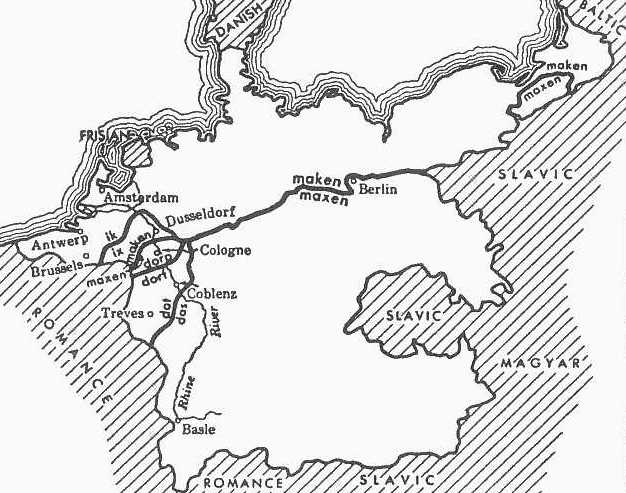
\includegraphics[width=0.8\textwidth]{3orth/images/hgcs.jpg}
  \caption[Bloomfield's isoglosses of the \acrshort{hgcs}.]{The Dutch-German speech area, with the isoglosses of several words containing [k/x], [t/s], and [p/f], from \textcite[344]{Blo_Language33}}
\label{fig:hgcsmap}
\end{figure}

\section{Geography and chronology of the shift}
\label{sec:geogr-chron-shift}

In the \gls{hgcs} we see a single shift of consonants, realised at different levels of completeness in different geographical locations. The merger of \lT\ and \xD\ in \gls{mw} has a temporal rather than a geographical transition zone. Yet the \gls{hgcs} did not occur overnight either:
\tqt{The spread of the High German shift northward, whatever its ultimate provenience, took place slowly. Although we have demonstrated the occurrence of shifted forms in Alemannic territory for as early as 600, we must not supose that this change was thoroughgoing and complete at this time. […] Bavarian documents preserve some non-High German forms well into the eighth century and even later. […] And not until the ninth century did the High German consonant shift reach the Middle Franconian dialect.}{Wat_History76}{62}
The fact that the \gls{hgcs} is executed to different levels of completeness along both temporal and geographical axes raises the question what the initial geographical extent of the merger of \lT\ to \xD\ was in \gls{mw}. This matter has remained unsolved in Part~\ref{part:orthography}, but it is obvious that some geographically intermediate stages must have existed for some amount of time.


\section{A review of \gls{mw} lenition rules}
\label{sec:cons-other-ideas}
Knowledge of when orthographical lenition of voiceless stops was introduced in Welsh, and knowledge of how scribes would emend older texts after this introduction makes it necessary to reconsider what we think we know of \gls{ow} and \gls{mw} grammar. I give an example below.

\Textcite[2]{schrijver_free_2010}, citing \textcite[18, 179]{evans_grammar_1964} and \textcite[193n]{morgan_y_1952}, states:
`Normally, if a plural subject noun follows the verb, the verb is in the 3sg […]. In early poetry, a plural verb may precede a plural subject, in which case the subject undergoes lenition.' Evidence for this archaic rule comes from the sentences below:
\begin{mwl}
  \mwc[ex:schrsubplv1]{CLlH 23.5a}{yn Aber Cuawc yt ganant gogeu}{In Aber Cuawg cuckoos sing}
  \mwc[ex:schrsubplv2]{AP 5.141}{ymgetwynt Gymry}{the Welsh will see to it}
\end{mwl}

The Canu Llywarch Hen poems are thought to have been composed in \gls{ow}, even though they survive in \gls{mw} orthography and in fourteenth century manuscripts, and the Book of Taliesin is shown to have added orthographic lenition of \mw[]{c}\footnote{See Section~\ref{sec:haycock}.} Having established that  lenition of voiceless stops was represented in the thirteenth century at the earliest, and having established that fourteenth-century scribes would add orthographical lenition of voiceless stops, we must amend Schrijver's (and Evans' and Morgan's) statement that nominal subjects of plural verbs undergo lenition in early poetry.

The fact of the matter is that lenition was probably added by the fourteenth-century manuscript scribes, rather than the original composers of the poem. It is indeed a feature of early poetry that plural verbs may have nominal subjects, but the lenition following it is not a feature of the early poetry itself, but rather a feature of the fourteenth-century manuscripts.

This means that those seeking to prove early poetry indeed had lenition of nominal subjects following plural verbs would either need to find a lenited nominal subject that has an initial consonant other than \mw[]{p, t, c}, or they would need to demonstrate that the orthographic lenition of these consonants indeed precedes the fourteenth century. In fact, \textcite[65--66]{van_development14} does not find subject lenition following plural verbs, but finds instances of non-lenition instead, including one case other than \mw[]{p, t, c}:
\mwcc[ex:vansluissubjlen]{RBH 641.38}{A gwrhau a \al{orugant gwyr} y iarllaeth y owein.}{And the noblemen did fealty to Owain’s earldom.}
This example comes from the Red Book of Hergest, dating from around 1400, and the tale itself is much later than the examples given by Schrijver. This curious mix of lenition and non-lenition remains an elusive puzzle, but all the pieces in this puzzle discovered so far belong to the \gls{mw} period, not the \gls{ow} period. Solving this puzzle would improve our knowledge of fourteenth-century Welsh, but it would not directly shed light upon the grammar of \gls{ow}\footnote{The examples quoted here curiously show lenition of voiceless stops, and non-lenition of other consonants. If this is indeed the pattern found, then subject lenition following plural verbs may not be representative of any synchronic stage of Welsh, but may instead be how fourteenth-century scribes thought the older stage operated. Then, when updating the orthography of lenition, they would use contemporary orthography for lenition, but non-contemporary rules governing lenition.}.

\section{Further research}
\label{sec:further-research}
The results presented in Part~\ref{part:orthography} give a few avenues for further research.

Chapter~\ref{cha:stemm-mwbuch-dewi}, established that manuscripts sharing lenition or lack thereof may have an amount of agreements beyond what may attributed to coincidence. Such patterns may be the result of shared inheritance of lenition, \ie a particular lenition fingerprint was transmitted into more than one descendant manuscript. Alternatively, however, a similar lenition fingerprint in two or more manuscripts may be the result of a common practice whereby lenition was added in different degrees in different grammatical environments. In order to establish a manuscript stemma based on the orthography of lenition, it is necessary to exclude the latter possibility. This latter possibility whereby shared conventions yield similar patterns of lenition may be excluded by identifying which grammatical environments lenite to different degrees than others. Then, it is possible to calculate whether lenition is modernised independently \emph{within} such a grammatical environment.

The unsolved challenge here is how to categorise types of lenition so that there is no overcategorisation or undercategorisation. If each particle that causes lenition is analysed independently, then sample sizes may be too low to detect a real-word significant correlation between manuscripts. If types of lenition are insufficiently divided, then the possibility of similar modernising practices causing similar patterns of lenition is not excluded. It is therefore necessary to understand which types of lenition are modernised in similar degrees to one another, and differently from other types of lenition. One possible way to do so is to divide between \gls{freelen} and \gls{contlen}. However, it is difficult to identify instances where \gls{freelen} was probably spoken yet not written, because this type of lenition was in flux. It is therefore necessary to find different ways to divide lenition in different classes. One way to do so may be by observing how different types of vowel-consonant or consonant-consonant combinations represent lenition.

Another unsolved issue is the geographical origin of the merger between \lT\ and \xD. In the temporal dimension, we may observe a pattern reminiscent of lexical diffusion with consecutive stages of the merger. In each successive stage, one lenited voiceless stop merges with its radical voiced counterpart and all mergers of previous stages persist. Because such a pattern is frequently observed within the field of dialectology, it is sensible to delve into thirteenth-century Welsh dialectology to see if a geographical as well as a temporal distribution may be found for the merger between \lT\ and \xD.

Yet another avenue for further research is Welsh from before the thirteenth century that survived in later manuscripts. As discussed in Section~\ref{sec:cons-other-ideas}, instances of lenition occurring in these early texts are often additions by later scribes. It would be worthwhile to review which rules governing lenition are thought of as early, yet only survive in comparatively late manuscripts. This may well lead to reconsideration of which lenition rules belong to which period. Lenition of nominal subjects following a plural verb seem to be an example of this.

% \section{Salesbury}
% \label{sec:salesbury}

% Fisher says:
% \tqt{Prefaced to the Prayer Book of 1567 is given his promised `Explanation of certaine wordes being quareled withall', from which we take the following:

%   `Vy-Dew for vynnuw, or vynyw, wherein D is now reteined, euen for the more significatiue expressing of the grace of the woord.

%   Vy-popul for vymhobl, to saue the word the les maimed.
  
%   Vy-troet for vynrhoed that the signification may be more apparent to the straunge Reader'.

%   It is clear that he wanted the reader --- the silent reader particularly --- to see what the original form of the word was, not only as regards the initial letter, but also in compounds, as we find. This method, he, of course, applied to the written word only, that it might be self-explanatory, and he never meant that any one should read aloud the text actually as written. Rather, he expected the reader to be himself able to introduce the proper mutations as i the spoken language, which any intelligent Welshman could and would do, and so read correctly without the imputed \textit{llediaith} and \textit{anghyfiaith}. By thus writing the words so as to indicate their supposed etymology, he also though that Welsh people of both North and South Wales would be the better able to understand them. In fact, he concerned himself with written Welsh only, and wanted to preserve the words `the les maimed' and `uncorrupt', without the mutations, regardless of the fact that the language as a living organism must grow and change with time, and in accordance with its own genius.
% }{Fis_Kynniver31}{xxxvii--xxxviii}

% \tqt{He treats compounds and words that are not compounds in the same manner. After all he was simply following the earlier orthography; \eg […] \textit{ympren croc, yn tuy vyntat, vygkorffi, amperffaith}.}{Fis_Kynniver31}{xxxix}

% Professor Richards' review:
% \tqt{In 1567, evidently in answer to his critics, he demanded, ``who \dots\ dyd ever wryte euery words as he sounded it?''. Another innovation was equally infelicitous. A stranger learning Welsh finds that the consonantal changes at the beginning of a word constitute his chief difficulty. Thus the word for father is written \textit{tad, dad, thad,} or \textit{nhad} according to its position in a sentence. Salesbury in every case used the radical or simplest form of such words. To judge from a sentence in the Dedication prexied to his Dictionary his object was to render it easier for readers to look up unusual words. The result was disastrous . His language appear clumsy and ungrammatical and the Welsh people would have none of it. Partly for this reason, and partly because it was superseded by Biship Richard Davies's translation of the whole Prayer Book in 1567, Kynnifer Llith a Ban was but little used.}{Ric_Welsh31}{}



%%% Local Variables:
%%% coding: utf-8
%%% mode: latex
%%% TeX-master: "../main"
%%% End:

\begin{spacing}{1}
  \appendix
  \chapter{Environments that cause lenition}
\label{cha:envir-that-cause}

Appendix~\ref{cha:database-lenition} and Appendix~\ref{cha:datab-lenit-mwbuch} contain all instances of lenition in the texts discussed in Part~\ref{part:orthography}. These databases contain instances of orthographical lenition, and instances where  lenition is expected, but not found. Here, all instances where lenition is expected but not found, and where lenition is found are discussed.

\section{Contact lenition}
\label{sec:contact-lenition-1}
Here, I list all types of contact lenition encountered. Here, I emend, \ie I argue lenition was in fact spoken even where it is not represented orthographically. Exceptions include unproductive categories such as lenition of nouns following a plural article \eg \mow{y bobl}, and cases where spirantisation may be expected instead of lenition, \eg verbs starting with \mow{p, t, c} following \mow{ni, na} or a compound thereof in a relative clause. The list is given in \gls{mow} orthography. 

\begin{itemize}
\item\mow{a} (interrogative particle): \textcite[§§~23, 196]{evans_grammar_1964}.
\item\mow{a} (verbal particle): \textcite[§§~23, 6, 192]{evans_grammar_1964}.
\item\mow{a} (vocative particle): \textcite[§~19]{evans_grammar_1964}.
\item\mow[to]{add}: \textcite[§~20]{evans_grammar_1964}.
\item\mow{-ai} (imperfect ending): \textcite[§~21]{evans_grammar_1964}; \textcite[42--45]{van_development14}.
\item\mow[second]{ail}: \textcite[§~249]{evans_grammar_1964}.
\item\mow[about]{am}: \textcite[§~20]{evans_grammar_1964}.
\item\mow[on]{ar}: \textcite[§~20]{evans_grammar_1964}.
\item\mow[to]{at}: \textcite[§~20]{evans_grammar_1964}.
\item\mow[with, by]{can}: \textcite[§~20]{evans_grammar_1964}.
\item\mow[although]{cani}: See \mow{ni}.
\item Equative \mow[as]{cyn}: \textcite[§§~22, 43]{evans_grammar_1964}.
\item\mow[around]{dam}: See \mow{am}.
\item\mow[two]{dau}: \textcite[§~20]{evans_grammar_1964}.
\item\mow[two]{dwy}: \textcite[§~20]{evans_grammar_1964}.
\item\mow[your]{dy}: \textcite[§~20]{evans_grammar_1964}.
\item\mow{-ed} (imperative ending): \textcite[§~21]{evans_grammar_1964}.
\item\mow[his]{ei}: \textcite[§~20]{evans_grammar_1964}.
\item feminine article \textcite[§~19]{evans_grammar_1964}.
\item feminine noun: \textcite[§§~19, 22]{evans_grammar_1964}.
\item\mow{-fu} (preterite ending): \textcite[§~21]{evans_grammar_1964}; \textcite[50--51]{van_development14}.
\item\mow[without]{heb}: \textcite[§~20]{evans_grammar_1964}.
\item\mow[until]{hyd}: \textcite[§~20]{evans_grammar_1964}.
\item\mow[his]{'i}: \textcite[§~20]{evans_grammar_1964}.
\item\mow[to]{i}: \textcite[§~20]{evans_grammar_1964}.
\item\mow[under]{is}: \textcite[§~20]{evans_grammar_1964}.
\item\mow[behold]{llyma}: \textcite[§~280]{evans_grammar_1964}; actually parenthesis i.e.\ free lenition.
\item\mow[so, as]{mor}: \textcite[§§~22, 41]{evans_grammar_1964}.
\item\mow{na} (negative particle): See \mow{ni}.
\item\mow[or]{neu}: \textcite[§~20]{evans_grammar_1964}.
\item\mow{ni} (negative particle): Before \mow{p, t, c} not included, except where represented; \textcite[§§~23, 24]{evans_grammar_1964}.
\item\mow{nir} (negative perfect particle): cf. \mow{rhy}.
\item\mow[from]{o}: \textcite[§~20]{evans_grammar_1964}.
\item\mow[there is]{oes}: \textcite[§~21]{evans_grammar_1964}; \textcite[39]{van_development14}.
\item\mow[until]{oni}: See \mow{ni}.
\item\mow[which]{pa}: \textcite[§~20]{evans_grammar_1964}.
\item\mow[when]{pan}: \textcite[§~23]{evans_grammar_1964}.
\item plural article: \textcite[10--11]{morgan_y_1952}.
\item\mow{rhy} (perfect particle): \textcite[§~23]{evans_grammar_1964}.
\item\mow[seven]{saith}: \textcite[§~20]{evans_grammar_1964}.
\item\mow[until, under]{tan}: \textcite[§~20]{evans_grammar_1964}.
\item\mow[your]{'th}: \textcite[§~20]{evans_grammar_1964}.
\item\mow[while]{tra}: \textcite[§~23]{evans_grammar_1964}.
\item\mow[over]{tros}: \textcite[§~20]{evans_grammar_1964}.
\item\mow[through]{trwy}: \textcite[§~20]{evans_grammar_1964}.
\item\mow[third]{trydedd}: \textcite[§~52]{evans_grammar_1964}.
\item Feminine \mow[one]{un}: \textcite[§~20]{evans_grammar_1964}.
\item\mow[above]{uwch}: \textcite[§~20]{evans_grammar_1964}.
\item\mow[against, by]{wrth}: \textcite[§~20]{evans_grammar_1964}.
\item\mow[eight]{wyth}: \textcite[§~20]{evans_grammar_1964}.
\item\mow{yd} (verbal particle): \textcite[§~23]{evans_grammar_1964}.
\item\mow{yn} (adverbial particle): \textcite[§~22]{evans_grammar_1964}.
\end{itemize}

\section{Free lenition}
\label{sec:free-lenition-1}
As many types of free lenition are in flux through the \gls{mw} period, I do not emend instances of free lenition, except where noted. That is, I do not take most instances where we could expect free lenition,  but where it is not written, to be an instance of \eg unwritten object lenition. This is because object lenition itself was not written consistently even where object lenition is known to have been written occasionally and where representation of lenition does not depend on consonant type.

Emended instances of free lenition are: apposition and preposed adjectives. \Gls{np} lenition and adverb lenition are sometimes included when the text as a whole employs these types of lenition consistently for other consonants.
\begin{itemize}
\item adverbial phrase \textcite[§~19, 22]{evans_grammar_1964}.
\item apposition: \textcite[§~19]{evans_grammar_1964}; \textcite[116--9, 122--3]{morgan_y_1952}; but especially \textcite{schrijver_free_2010}. Examples include \mw[Macsen the lord]{Macsen \al{W}ledic}, and vocative expressions without the vocative particle, \eg \mw[What is this, Margaret?]{Pa beth yw hynn, \al{V}argret?}.
\item compound: \textcite[§~20, 22]{evans_grammar_1964}. 
\item existential verb:  \textcite[29--30]{van_development14}. Any inflected form of \mow[to be]{bod} may cause lenition to its subject when it has the semantics of an existential verb, analogous to lenition after \mow[there is]{oes}.
\item \gls{np} lenition: \textcite[§~21]{evans_grammar_1964}.
\item object of destination: \textcite[227]{morgan_y_1952}; \textcite[§~21]{evans_grammar_1964}. 
\item object lenition: \textcite[§~21]{evans_grammar_1964}.
\item parenthesis: \textcite[429]{morgan_y_1952}, \textcite[§~21]{evans_grammar_1964}, \textcite[5--6]{schrijver_free_2010}.
\item preposed adjective: \textcite[35]{morgan_y_1952}. Often difficult to distinguish from preposed nouns, because nouns may be used as adjectives and vice versa. Mostly found in poetry, except in the case of adjectives such as \mw[old]{hen} which always precede the noun  they specify.
\item preposed noun: a noun that stands in a genitival relationship with the noun following usually causes lenition, \eg \mow[leaves of Autumn]{Hydref ddail}~\autocite{daniel_cyfuniadau_2003}.
\item subject to plural verb: \textcite[§~21]{evans_grammar_1964}; \textcite[2]{schrijver_free_2010}, although \textcite{van_development14} fails to find lenition in this environment.
\end{itemize}


%%% Local Variables:
%%% coding: utf-8
%%% mode: latex
%%% TeX-master: "../main"
%%% End:

  \chapter{Database of lenition}
\label{cha:database-lenition}
This Appendix lists instances where lenition is either expected or lenition found in all texts discussed in Part~\ref{part:orthography}, with the exception of Chapter~\ref{cha:stemm-mwbuch-dewi}, which has a different structure for its database.


\begin{center}
\section{Scribe X86}
\label{sec:x86}
\begin{longtable}{addwllwl}
  \toprule
  \tch{MS} & \tch{p./f.} & \tch{l.} & \tch{Word} & \tch{Cause lenition} & \tch{len.} & \tch{\gls{C}} & \tch{\acrshort{RE}} \\
  \midrule
  \endhead
  \bottomrule
  \endfoot
bt & 13 & 3  & genhyn & Petrification & \TRUE & c  & \TRUE \\
bt & 13 & 7  & Gaer & \mw{hyt} & \TRUE & c  & \FALSE \\
bt & 13 & 7  & Weir & fem.\ noun & \TRUE & g  & \FALSE \\
bt & 13 & 8  & goꝛuoled & obj. & \FALSE & g  & \FALSE \\
bt & 13 & 10 & genhyn & Petrification & \TRUE & c  & \TRUE \\
bt & 13 & 11 & uyd & [\mw{a}] & \TRUE & b  & \FALSE \\
bt & 13 & 17 & gỽynyn & \mw{a} & \TRUE & c  & \FALSE \\
bt & 13 & 19 & telhyn & \mw{a} & \FALSE & t  & \FALSE \\
bt & 13 & 19 & ỽr & \gls{np} & \TRUE & g  & \FALSE \\
bt & 13 & 20 & talei & \mw{a} & \FALSE & t  & \FALSE \\
bt & 13 & 21 & eir & \mw{a} [\mw{o}] & \TRUE & g  & \FALSE \\
bt & 13 & 24 & wydynt & \mw{ny} & \TRUE & g  & \FALSE \\
bt & 13 & 25 & treiglynt & \mw{py} & \FALSE & t  & \FALSE \\
bt & 13 & 25 & pꝛynaſſant & \mw{pan} & \FALSE & p  & \FALSE \\
bt & 13 & 25 & Danet & obj. & \TRUE & t  & \FALSE \\
bt & 13 & 26 & gan & Petrification & \TRUE & c  & \TRUE \\
bt & 14 & 3  & wiraỽt & prep.\ adj. & \TRUE & g  & \FALSE \\
bt & 14 & 3  & ved & \mw{o} & \TRUE & m  & \FALSE \\
bt & 14 & 6  & uyd & \mw{pan} & \TRUE & b  & \FALSE \\
bt & 14 & 8  & bỽyller & \mw{a} & \TRUE & p  & \FALSE \\
bt & 14 & 8  & Vꝛython & fem.\ noun & \TRUE & b  & \FALSE \\
bt & 14 & 11 & eir & \mw{a} [\mw{o}] & \TRUE & g  & \FALSE \\
bt & 14 & 13 & goꝛ & \mw{un} & \TRUE & c  & \FALSE \\
bt & 14 & 13 & gyghoꝛ & \mw{un} & \TRUE & c  & \FALSE \\
bt & 14 & 18 & lan & \mw{am} & \TRUE & g  & \FALSE \\
bt & 14 & 19 & vydinaỽr & prep.\ adj. & \TRUE & b  & \FALSE \\
bt & 14 & 20 & Gỽy & \mw{am} & \FALSE & g  & \FALSE \\
bt & 14 & 21 & peurllyn & \mw{am} & \FALSE & p  & \FALSE \\
bt & 14 & 22 & kynyrche/it & prep noun & \FALSE & c  & \FALSE \\
bt & 14 & 23 & von & \mw{ỽrth} & \TRUE & b  & \FALSE \\
bt & 14 & 26 & goet & \mw{trỽy} & \TRUE & c  & \FALSE \\
bt & 14 & 26 & uỽꝛch & \mw{trỽy} & \TRUE & b  & \FALSE \\
bt & 15 & 1  & tir & \mw{y} ‘to' & \FALSE & t  & \FALSE \\
bt & 15 & 2  & laỽ & \mw{trỽy} & \TRUE & ll & \FALSE \\
bt & 15 & 2  & gyghoꝛ & fem.\ noun & \TRUE & c  & \FALSE \\
bt & 15 & 3  & Geri & fem.\ noun & \TRUE & c  & \FALSE \\
bt & 15 & 6  & watwar & prep.\ adj. & \TRUE & g  & \FALSE \\
bt & 15 & 8  & oꝛol/chant & \mw{a} & \TRUE & g  & \FALSE \\
bt & 15 & 9  & kyneircheit & prep noun & \FALSE & c  & \FALSE \\
bt & 15 & 11 & vedyc & \mw{y} ‘to' & \TRUE & m  & \FALSE \\
bt & 15 & 11 & mỽyn & parenthesis & \FALSE & m  & \FALSE \\
bt & 15 & 12 & wnaant & \mw{a} & \TRUE & g  & \FALSE \\
bt & 15 & 13 & wnant & \mw{a} & \TRUE & g  & \FALSE \\
bt & 15 & 15 & ỽdant & \mw{a} & \TRUE & g  & \FALSE \\
bt & 15 & 17 & gerd & \mw{a} & \TRUE & c  & \FALSE \\
bt & 15 & 17 & genhyn & Petrification & \TRUE & c  & \TRUE \\
bt & 15 & 19 & baladyr & \mw{yn} & \TRUE & p  & \FALSE \\
bt & 15 & 19 & gan & Petrification & \TRUE & c  & \TRUE \\
bt & 15 & 21 & dꝛoſ & Petrification & \TRUE & t  & \TRUE \\
bt & 15 & 22 & rud & \mw{ar} & \TRUE & g  & \FALSE \\
bt & 15 & 23 & Gaer & \mw{hyt} & \TRUE & c  & \FALSE \\
bt & 15 & 24 & Wynt & fem.\ noun & \TRUE & g  & \FALSE \\
bt & 15 & 25 & Gymry & apposition & \TRUE & c  & \FALSE \\
bt & 15 & 25 & trindaỽt & fem.\ art & \FALSE & t  & \FALSE \\
bt & 15 & 26 & gynt & adv.\ phrase & \TRUE & c  & \FALSE \\
bt & 16 & 3  & genhyn & Petrification & \TRUE & c  & \TRUE \\
bt & 16 & 3  & talet & \mw{heb} & \FALSE & t  & \FALSE \\
bt & 16 & 3  & dynget & \mw{o} & \TRUE & t  & \FALSE \\
bt & 16 & 4  & geffyn & \mw{a} & \TRUE & c  & \FALSE \\
bt & 16 & 4  & veibon & prep.\ adj. & \TRUE & m  & \FALSE \\
bt & 16 & 7  & gỽſſyl & Unsure & \TRUE & c  & \FALSE \\
bt & 16 & 7  & coꝛ & \mw{un} & \FALSE & c  & \FALSE \\
bt & 16 & 7  & gyg/hoꝛ & Unsure & \TRUE & c  & \FALSE \\
bt & 16 & 8  & lloſcit & prep noun & \FALSE & ll & \FALSE \\
bt & 16 & 9  & luyd & prep.\ adj. & \TRUE & ll & \FALSE \\
bt & 16 & 9  & beunyd & adv.\ phrase & \TRUE & p  & \FALSE \\
bt & 16 & 10 & ỽyr & \mw{ny} & \TRUE & g  & \FALSE \\
bt & 16 & 10 & uyd & [\mw{a}] & \TRUE & b  & \FALSE \\
bt & 16 & 11 & gyfarth & obj. & \TRUE & c  & \FALSE \\
bt & 16 & 11 & vynyd & \mw{o} & \TRUE & m  & \FALSE \\
bt & 16 & 11 & talu & \mw{ẏ} ‘to' & \FALSE & t  & \FALSE \\
bt & 16 & 13 & coꝛff & obj. & \FALSE & c  & \FALSE \\
bt & 16 & 13 & gilyd & \mw{y} ‘his' & \TRUE & c  & \FALSE \\
bt & 16 & 17 & galaned & subj.\ pl.\ v. & \TRUE & c  & \FALSE \\
bt & 16 & 18 & treth & fem.\ art & \FALSE & t  & \FALSE \\
bt & 16 & 18 & gỽerth & \mw{ar} & \FALSE & g  & \FALSE \\
bt & 16 & 18 & beunyd & adv.\ phrase & \TRUE & p  & \FALSE \\
bt & 16 & 19 & gennadeu & prep.\ adj. & \TRUE & c  & \FALSE \\
bt & 16 & 19 & luyd & prep.\ adj. & \TRUE & ll & \FALSE \\
bt & 16 & 20 & kyfergyr & \mw{trỽy} & \FALSE & c  & \FALSE \\
bt & 16 & 20 & gyweir & \mw{yn} & \TRUE & c  & \FALSE \\
bt & 16 & 20 & gyteir & adv.\ phrase & \TRUE & c  & \FALSE \\
bt & 16 & 21 & gẏtſon & adv.\ phrase & \TRUE & c  & \FALSE \\
bt & 16 & 21 & gytffyd & adv.\ phrase & \TRUE & c  & \FALSE \\
bt & 16 & 21 & peri & \mw{y} ‘to' & \FALSE & p  & \FALSE \\
bt & 16 & 22 & gynnullant & \mw{a} & \TRUE & c  & \FALSE \\
bt & 16 & 23 & tywyſſaỽ & \mw{y} ‘to' & \FALSE & t  & \FALSE \\
bt & 16 & 23 & liein/gant & \mw{trỽy} & \TRUE & ll & \FALSE \\
bt & 16 & 24 & genhyn & Petrification & \TRUE & c  & \TRUE \\
bt & 16 & 25 & gat & fem.\ art & \TRUE & c  & \FALSE \\
bt & 16 & 26 & geiſſyſſant & [\mw{a}] & \TRUE & c  & \FALSE \\
bt & 17 & 1  & wlad & fem.\ art & \TRUE & g  & \FALSE \\
bt & 17 & 2  & vꝛo & \mw{py} & \TRUE & b  & \FALSE \\
bt & 17 & 3  & genhyn & Petrification & \TRUE & c  & \TRUE \\
bt & 17 & 4  & wir & \mw{o} & \TRUE & g  & \FALSE \\
bt & 17 & 4  & vꝛeint & \mw{neu} & \TRUE & b  & \FALSE \\
bt & 17 & 6  & Gymry & subj.\ pl.\ v. & \TRUE & c  & \FALSE \\
bt & 17 & 7  & talhont & \mw{pan} & \FALSE & t  & \FALSE \\
bt & 17 & 8  & gỽerth & prep.\ adj. & \FALSE & g  & \FALSE \\
bt & 17 & 9  & garant & [\mw{a}] & \TRUE & c  & \FALSE \\
bt & 17 & 12 & lygheſ & parenthesis & \TRUE & ll & \FALSE \\
bt & 17 & 13 & gat & fem.\ art & \TRUE & c  & \FALSE \\
bt & 17 & 13 & gỽyr & parenthesis & \FALSE & g  & \FALSE \\
bt & 17 & 14 & Pꝛydein & \mw{o} & \FALSE & p  & \FALSE \\
bt & 17 & 14 & virein & parenthesis & \TRUE & m  & \FALSE \\
bt & 17 & 14 & luyd & prep.\ adj. & \TRUE & ll & \FALSE \\
bt & 17 & 15 & Lydaỽ & \mw{o} & \TRUE & ll & \FALSE \\
bt & 17 & 15 & pꝛydaỽ & parenthesis & \FALSE & p  & \FALSE \\
bt & 17 & 15 & gywiethyd & prep.\ adj. & \TRUE & c  & \FALSE \\
bt & 17 & 15 & katueirch & \mw{ar} & \FALSE & c  & \FALSE \\
bt & 17 & 16 & pop & \mw{o} & \FALSE & p  & \FALSE \\
bt & 17 & 18 & gyweithyd & prep.\ adj. & \TRUE & c  & \FALSE \\
bt & 17 & 24 & vꝛaỽt & \mw{hyt} & \TRUE & b  & \FALSE \\
bt & 17 & 25 & oꝛſegyn & \mw{deu} & \TRUE & g  & \FALSE \\
bt & 17 & 25 & pleit & \mw{o} & \FALSE & p  & \FALSE \\
bt & 17 & 26 & gedaỽl & \mw{deu} & \TRUE & c  & \FALSE \\
bt & 17 & 26 & gỽlatwarthegyd & prep.\ adj. & \FALSE & g  & \FALSE \\
bt & 18 & 1  & baraỽt & prep.\ adj. & \TRUE & p  & \FALSE \\
bt & 18 & 2  & luyd & prep.\ adj. & \TRUE & ll & \FALSE \\
bt & 18 & 3  & beunyd & adv.\ phrase & \TRUE & p  & \FALSE \\
bt & 18 & 4  & Vynaỽ & \mw{o} & \TRUE & m  & \FALSE \\
bt & 18 & 4  & Lydaỽ & \mw{hyt} & \TRUE & ll & \FALSE \\
bt & 18 & 5  & vyd & \mw{yt} & \TRUE & b  & \FALSE \\
bt & 18 & 5  & Danet & \mw{hyt} & \TRUE & t  & \FALSE \\
bt & 18 & 5  & bieiuyd & [\mw{a}] & \TRUE & p  & \FALSE \\
bt & 18 & 5  & Waỽl & \mw{o} & \TRUE & g  & \FALSE \\
bt & 18 & 6  & Weryt & \mw{hyt} & \TRUE & g  & \FALSE \\
bt & 18 & 7  & gynhon & \mw{ar} & \FALSE & g  & \FALSE \\
bt & 18 & 8  & Ỽydyl & subj.\ pl.\ v. & \TRUE & g  & \FALSE \\
bt & 18 & 9  & Gymry & subj.\ pl.\ v. & \TRUE & c  & \FALSE \\
bt & 18 & 9  & kadyr & obj. & \FALSE & c  & \FALSE \\
bt & 18 & 9  & gyweithyd & prep.\ adj. & \TRUE & c  & \FALSE \\
bt & 18 & 10 & gỽꝛỽf & \mw{am} & \TRUE & c  & \FALSE \\
bt & 18 & 10 & ge/dỽyſ & \mw{ry} & \TRUE & c  & \FALSE \\
bt & 18 & 11 & pop & \mw{y} ‘to' & \FALSE & p  & \FALSE \\
bt & 18 & 12 & gan & Petrification & \TRUE & c  & \TRUE \\
bt & 18 & 12 & gilyd & \mw{y} ‘his' & \TRUE & c  & \FALSE \\
bt & 18 & 12 & alwaỽꝛ & \mw{ny} & \TRUE & g  & \FALSE \\
bt & 18 & 13 & gynifwyr & \mw{yn} & \TRUE & c  & \FALSE \\
bt & 18 & 14 & gyfnewitwyr & \mw{e} ‘his' & \TRUE & c  & \FALSE \\
bt & 18 & 15 & uyd & [\mw{a}] & \TRUE & b  & \FALSE \\
bt & 18 & 15 & gymỽyeit & fem.\ noun & \TRUE & c  & \FALSE \\
bt & 18 & 16 & galaned & subj.\ pl.\ v. & \TRUE & c  & \FALSE \\
bt & 18 & 17 & vyd & [\mw{a}] & \TRUE & b  & \FALSE \\
bt & 18 & 17 & gychwyn & \mw{ar} & \TRUE & c  & \FALSE \\
bt & 18 & 19 & voꝛ & \mw{ar} & \TRUE & m  & \FALSE \\
bt & 18 & 19 & peunyd & adv.\ phrase & \FALSE & p  & \FALSE \\
bt & 18 & 20 & vꝛaỽt & \mw{hyt} & \TRUE & b  & \FALSE \\
bt & 18 & 20 & lyfraỽꝛ & obj. & \TRUE & ll & \FALSE \\
bt & 18 & 21 & bꝛydyd & prep.\ adj. & \TRUE & p  & \FALSE \\
bt & 18 & 22 & greỽys & \mw{a} & \TRUE & c  & \FALSE \\
bt & 18 & 24 & Kaer & fem.\ noun & \FALSE & c  & \FALSE \\
bt & 18 & 25 & ỽyỽ & \mw{ny} & \TRUE & g  & \FALSE \\
bt & 18 & 25 & wellyc & \mw{ny} & \TRUE & g  & \FALSE \\
bt & 28 & 22 & ofrỽy & Unsure & \TRUE & g  & \FALSE \\
bt & 28 & 23 & tarrỽy & \mw{a} & \FALSE & t  & \FALSE \\
bt & 28 & 23 & treiſ & \mw{a} & \FALSE & t  & \FALSE \\
bt & 28 & 23 & dꝛoſ & Petrification & \TRUE & t  & \TRUE \\
bt & 28 & 23 & voꝛdỽy & \mw{dꝛoſ} & \TRUE & m  & \FALSE \\
bt & 28 & 23 & prꝛen & \mw{py} & \FALSE & p  & \FALSE \\
bt & 28 & 24 & vo & \mw{a} & \TRUE & b  & \FALSE \\
bt & 28 & 25 & uỽy & \gls{np} & \TRUE & m  & \FALSE \\
bt & 28 & 26 & Vathonỽy & fem.\ noun & \TRUE & m  & \FALSE \\
bt & 29 & 1  & tyfỽy & \mw{pan} & \FALSE & t  & \FALSE \\
bt & 29 & 2  & wledych/ỽy & \mw{pan} & \TRUE & g  & \FALSE \\
bt & 29 & 3  & trei & \mw{troſ} & \FALSE & t  & \FALSE \\
bt & 29 & 3  & traeth & \mw{throſ} & \FALSE & t  & \FALSE \\
bt & 29 & 4  & pennaeth & prep.\ adj. & \FALSE & p  & \FALSE \\
bt & 29 & 4  & pymhet & fem.\ art & \FALSE & p  & \FALSE \\
bt & 29 & 5  & Pꝛydein & \mw{ar} & \FALSE & p  & \FALSE \\
bt & 29 & 5  & ui & \mw{a} & \TRUE & b  & \FALSE \\
bt & 29 & 6  & ui & \mw{a} & \TRUE & b  & \FALSE \\
bt & 29 & 8  & vein & prep.\ adj. & \TRUE & m  & \FALSE \\
bt & 29 & 8  & wyr & \mw{ar} & \TRUE & g  & \FALSE \\
bt & 29 & 9  & gyg/ein & \mw{a} & \TRUE & c  & \FALSE \\
bt & 29 & 10 & gerd & \mw{ar} & \TRUE & c  & \FALSE \\
bt & 29 & 11 & gygein & \mw{yt} & \TRUE & c  & \FALSE \\
bt & 29 & 11 & tynnu & \mw{y} ‘to' & \FALSE & t  & \FALSE \\
bt & 29 & 12 & wan & \mw{y} ‘to' & \TRUE & g  & \FALSE \\
bt & 29 & 12 & tyruu & \mw{y} ‘to' & \FALSE & t  & \FALSE \\
bt & 29 & 12 & w/naeth & \mw{a} & \TRUE & g  & \FALSE \\
bt & 29 & 13 & wiſc & \mw{o} & \TRUE & g  & \FALSE \\
bt & 29 & 14 & uuant & \mw{yt} & \TRUE & b  & \FALSE \\
bt & 29 & 15 & lan & \mw{ar} & \TRUE & g  & \FALSE \\
bt & 29 & 15 & uu & \mw{yt} & \TRUE & b  & \FALSE \\
bt & 29 & 15 & wnel & \mw{pan} & \TRUE & g  & \FALSE \\
bt & 29 & 15 & kamualhau & obj. & \FALSE & c  & \FALSE \\
bt & 29 & 16 & lam & \mw{i} ‘to' & \TRUE & ll & \FALSE \\
bt & 29 & 16 & lam & \mw{o} & \TRUE & ll & \FALSE \\
bt & 29 & 16 & keỽſſit & [\mw{a}] & \FALSE & c  & \FALSE \\
bt & 29 & 17 & gaho & \mw{nyr} & \TRUE & c  & \FALSE \\
bt & 29 & 17 & ỽc & \mw{a} & \TRUE & g  & \FALSE \\
bt & 29 & 19 & wyl & \mw{a} & \TRUE & g  & \FALSE \\
bt & 29 & 22 & biewyd & [\mw{a}] & \TRUE & p  & \FALSE \\
bt & 29 & 22 & gyneiluoaỽc & obj. & \TRUE & c  & \FALSE \\
bt & 29 & 25 & bꝛydein & \mw{o} & \TRUE & p  & \FALSE \\
bt & 29 & 26 & gofein & prep noun & \TRUE & c  & \FALSE \\
bt & 29 & 26 & berth & \mw{o} & \TRUE & p  & \FALSE \\
bt & 29 & 26 & ky/uerbyn & obj. & \FALSE & c  & \FALSE \\
bt & 30 & 2  & lyghes & \mw{y} ‘to' & \TRUE & ll & \FALSE \\
bt & 30 & 2  & beleidyr & \mw{o} & \TRUE & p  & \FALSE \\
bt & 30 & 2  & bleigheit & \mw{o} & \TRUE & p  & \FALSE \\
bt & 30 & 2  & pꝛen/wres & Unsure & \FALSE & Unsure & \FALSE \\
bt & 30 & 3  & paỽb & \mw{y} ‘to' & \FALSE & p  & \FALSE \\
bt & 30 & 3  & trachwres & \mw{y} ‘his' & \FALSE & t  & \FALSE \\
bt & 30 & 4  & gadeu & \mw{o} & \TRUE & c  & \FALSE \\
bt & 30 & 6  & vꝛetrỽyn & fem.\ noun & \TRUE & b  & \FALSE \\
bt & 30 & 7  & wres & \mw{trỽy} & \TRUE & g  & \FALSE \\
bt & 30 & 7  & tan & prep.\ adj. & \FALSE & t  & \FALSE \\
bt & 30 & 7  & trachwres & \mw{y} ‘his' & \FALSE & t  & \FALSE \\
bt & 30 & 10 & veibon & \mw{y} ‘to' & \TRUE & m  & \FALSE \\
bt & 30 & 11 & alon & \mw{dy} & \TRUE & g  & \FALSE \\
bt & 30 & 11 & uraỽt & \mw{ad} & \TRUE & b  & \FALSE \\
bt & 30 & 14 & gan & Petrification & \TRUE & c  & \TRUE \\
bt & 30 & 14 & waỽꝛ & \mw{gan} & \TRUE & g  & \FALSE \\
bt & 30 & 18 & wnaỽ & \mw{a} & \TRUE & g  & \FALSE \\
bt & 30 & 22 & gaenaỽc & prep.\ adj. & \TRUE & c  & \FALSE \\
bt & 30 & 22 & wyl & \mw{ny} & \TRUE & g  & \FALSE \\
bt & 30 & 22 & welas & \mw{ny} & \TRUE & g  & \FALSE \\
bt & 30 & 26 & wiraỽt & prep noun & \TRUE & g  & \FALSE \\
bt & 31 & 1  & gefyn & \mw{ar} & \TRUE & c  & \FALSE \\
bt & 31 & 2  & gaer & prep noun & \TRUE & c  & \FALSE \\
bt & 31 & 3  & Venei & \mw{ar} & \TRUE & m  & \FALSE \\
bt & 31 & 3  & gyflogaỽt & prep noun & \TRUE & c  & \FALSE \\
bt & 31 & 4  & Gonỽy & \mw{ar} & \TRUE & c  & \FALSE \\
bt & 31 & 5  & baraỽt & Unsure & \TRUE & p  & \FALSE \\
bt & 31 & 7  & dꝛoch & Unsure & \TRUE & t  & \FALSE \\
bt & 31 & 7  & dꝛymluaỽc & Unsure & \TRUE & t  & \FALSE \\
bt & 31 & 8  & kat & prep noun & \FALSE & c  & \FALSE \\
bt & 31 & 8  & tri & \mw{am} & \FALSE & t  & \FALSE \\
bt & 31 & 9  & pop & \mw{o} & \FALSE & p  & \FALSE \\
bt & 31 & 10 & vꝛe & prep noun & \TRUE & b  & \FALSE \\
bt & 31 & 10 & varnhaỽt & [\mw{a}] & \TRUE & b  & \FALSE \\
bt & 31 & 11 & ynt & \mw{o} & \TRUE & g  & \FALSE \\
bt & 31 & 15 & gan & Petrification & \TRUE & c  & \TRUE \\
bt & 31 & 15 & verch & \mw{gan} & \TRUE & m  & \FALSE \\
bt & 31 & 15 & vꝛaỽt & \mw{y} ‘his' & \TRUE & b  & \FALSE \\
bt & 31 & 16 & lin & \mw{o} & \TRUE & ll & \FALSE \\
bt & 31 & 18 & lef & \mw{ỽꝛth} & \TRUE & ll & \FALSE \\
bt & 31 & 19 & bedꝛydant & \mw{o} & \TRUE & p  & \FALSE \\
bt & 31 & 20 & leſni & \mw{-i} & \TRUE & g  & \FALSE \\
bt & 31 & 20 & laſwaỽt & \mw{o} & \TRUE & g  & \FALSE \\
bt & 38 & 11 & Galchuynyd & \mw{o} & \TRUE & c  & \FALSE \\
bt & 38 & 13 & leu & \mw{y} ‘to' & \TRUE & ll & \FALSE \\
bt & 38 & 13 & vedyd & \mw{y} ‘to' & \TRUE & b  & \FALSE \\
bt & 38 & 13 & lawen & Unsure & \TRUE & ll & \FALSE \\
bt & 38 & 14 & gynnyd & prep.\ adj. & \TRUE & c  & \FALSE \\
bt & 38 & 15 & Gymry & \mw{o} & \TRUE & c  & \FALSE \\
bt & 38 & 18 & vꝛo & \mw{dy} & \TRUE & b  & \FALSE \\
bt & 38 & 19 & vo & \mw{yt} & \TRUE & b  & \FALSE \\
bt & 38 & 19 & gyrchaſſam & \mw{pan} & \TRUE & c  & \FALSE \\
bt & 38 & 19 & trỽy/det & obj. & \FALSE & t  & \FALSE \\
bt & 38 & 20 & tir & \mw{ar} & \FALSE & t  & \FALSE \\
bt & 38 & 20 & veinwen & fem.\ noun & \TRUE & m  & \FALSE \\
bt & 38 & 21 & Gludỽys & \mw{o} & \TRUE & c  & \FALSE \\
bt & 38 & 22 & vꝛo & prep noun & \TRUE & b  & \FALSE \\
bt & 38 & 23 & Vabon & prep.\ adj. & \TRUE & m  & \FALSE \\
bt & 38 & 23 & vꝛo & prep.\ adj. & \TRUE & b  & \FALSE \\
bt & 38 & 23 & biỽ & obj. & \FALSE & b  & \FALSE \\
bt & 38 & 24 & vꝛo & \mw{y} ‘his' & \TRUE & b  & \FALSE \\
bt & 38 & 26 & lenyn & prep.\ adj. & \TRUE & ll & \FALSE \\
bt & 39 & 2  & welei & \mw{a} & \TRUE & g  & \FALSE \\
bt & 39 & 2  & Vabon & \ei & \TRUE & m  & \FALSE \\
bt & 39 & 2  & ranwen & \mw{ar} & \TRUE & g  & \FALSE \\
bt & 39 & 4  & galaned & \mw{heb} & \TRUE & c  & \FALSE \\
bt & 39 & 5  & gyfarfot & \mw{o} & \TRUE & c  & \FALSE \\
bt & 39 & 5  & Vabon & fem.\ noun & \TRUE & m  & \FALSE \\
bt & 39 & 6  & gỽehenyt & prep noun & \FALSE & g  & \FALSE \\
bt & 39 & 6  & ban & Petrification & \TRUE & p  & \TRUE \\
bt & 39 & 7  & tat & \mw{y} ‘his' & \FALSE & t  & \FALSE \\
bt & 39 & 7  & galch & \ei & \TRUE & c  & \FALSE \\
bt & 39 & 10 & gyfỽyre & prep.\ adj. & \TRUE & c  & \FALSE \\
bt & 39 & 10 & gnaỽt & \mw{ar} & \TRUE & c  & \FALSE \\
bt & 39 & 11 & leu & \mw{o} & \TRUE & ll & \FALSE \\
bt & 39 & 11 & tired & prep.\ adj. & \FALSE & t  & \FALSE \\
bt & 39 & 12 & ogyfeirch & \mw{th} & \TRUE & g  & \FALSE \\
bt & 39 & 12 & och/wynogyon & Unsure & \TRUE & g  & \FALSE \\
bt & 39 & 13 & gatuaon & \mw{y} ‘his' & \TRUE & c  & \FALSE \\
bt & 39 & 14 & ban & Petrification & \TRUE & p  & \TRUE \\
bt & 39 & 14 & berit & \mw{pan} & \TRUE & p  & \FALSE \\
bt & 39 & 15 & gyfaruot & \mw{o} & \TRUE & c  & \FALSE \\
bt & 39 & 16 & vꝛein & \mw{y} ‘his' & \TRUE & b  & \FALSE \\
bt & 39 & 17 & ban & Petrification & \TRUE & p  & \TRUE \\
bt & 39 & 18 & uolch & fem.\ noun & \TRUE & b  & \FALSE \\
bt & 39 & 18 & ỽrthyat & prep noun & \TRUE & g  & \FALSE \\
bt & 39 & 19 & trablud & prep noun & \FALSE & t  & \FALSE \\
bt & 39 & 19 & reei & \mw{ny} & \TRUE & g  & \FALSE \\
bt & 39 & 19 & warthec & \ei & \TRUE & g  & \FALSE \\
bt & 39 & 20 & yrat & prep.\ adj. & \TRUE & g  & \FALSE \\
bt & 39 & 20 & goꝛgol/che\abbr{i} & [\mw{a}] & \FALSE & g  & \FALSE \\
bt & 39 & 21 & gỽarthaf & \ei & \FALSE & g  & \FALSE \\
bt & 39 & 22 & greulet & fem.\ noun & \TRUE & c  & \FALSE \\
bt & 39 & 22 & genem & prep noun & \TRUE & c  & \FALSE \\
bt & 39 & 22 & Wenhỽys & fem.\ noun & \TRUE & g  & \FALSE \\
bt & 39 & 24 & urỽydyr & prep.\ adj. & \TRUE & b  & \FALSE \\
bt & 39 & 24 & gyffeſtraỽn & prep.\ adj. & \TRUE & c  & \FALSE \\
bt & 39 & 26 & irat & \mw{a} [\mw{o}] & \TRUE & g  & \FALSE \\
bt & 40 & 1  & ỽyr & subj.\ pl.\ v. & \TRUE & g  & \FALSE \\
bt & 45 & 11 & ket & obj. & \FALSE & c  & \FALSE \\
bt & 45 & 14 & karrec & fem.\ noun & \FALSE & c  & \FALSE \\
bt & 45 & 15 & kynan & \mw{cant} & \FALSE & c  & \FALSE \\
bt & 45 & 17 & Ỽy & \mw{ar} & \TRUE & g  & \FALSE \\
bt & 45 & 17 & ladet & \mw{a} & \TRUE & ll & \FALSE \\
bt & 45 & 18 & maỽꝛ & fem.\ noun & \FALSE & m  & \FALSE \\
bt & 45 & 18 & tec & fem.\ noun & \FALSE & t  & \FALSE \\
bt & 45 & 19 & molet & \mw{a} [\mw{o}] & \FALSE & m  & \FALSE \\
bt & 45 & 19 & gỽoꝛgret & \mw{a} [\mw{o}] & \FALSE & g  & \FALSE \\
bt & 45 & 20 & gerdet & \mw{ar} & \TRUE & c  & \FALSE \\
bt & 45 & 21 & welet & \mw{ry} & \TRUE & g  & \FALSE \\
bt & 45 & 21 & biỽ & \mw{y} ‘his' & \FALSE & b  & \FALSE \\
bt & 45 & 24 & gynan & \mw{o} & \TRUE & c  & \FALSE \\
bt & 45 & 25 & lydan & fem.\ noun & \TRUE & ll & \FALSE \\
bt & 45 & 26 & godaran & fem.\ noun & \FALSE & g  & \FALSE \\
bt & 46 & 3  & lydan & fem.\ noun & \TRUE & ll & \FALSE \\
bt & 46 & 3  & gochvan & \mw{y} ‘his' & \FALSE & g  & \FALSE \\
bt & 46 & 4  & gynan & \mw{dy} ‘to' & \TRUE & c  & \FALSE \\
bt & 56 & 14 & gan & Petrification & \TRUE & c  & \TRUE \\
bt & 56 & 14 & wledic & \mw{am} & \TRUE & g  & \FALSE \\
bt & 56 & 15 & gỽarthegyd & prep.\ adj. & \FALSE & g  & \FALSE \\
bt & 56 & 16 & teyrned & obj. & \FALSE & t  & \FALSE \\
bt & 56 & 19 & kyuygyd & prep noun & \FALSE & c  & \FALSE \\
bt & 56 & 20 & oꝛmes & \mw{dy} & \TRUE & g  & \FALSE \\
bt & 56 & 21 & dꝛos & Petrification & \TRUE & t  & \TRUE \\
bt & 56 & 21 & wyr & obj. & \TRUE & g  & \FALSE \\
bt & 56 & 23 & tỽrỽf & obj. & \FALSE & t  & \FALSE \\
bt & 56 & 26 & wyr & obj. & \TRUE & g  & \FALSE \\
bt & 57 & 1  & tanc & obj. & \FALSE & t  & \FALSE \\
bt & 57 & 1  & gan & Petrification & \TRUE & c  & \TRUE \\
bt & 57 & 3  & gynrein & \mw{y} ‘his' & \TRUE & c  & \FALSE \\
bt & 57 & 3  & kyỽym don & Unsure & \FALSE & c  & \FALSE \\
bt & 57 & 4  & wyr & obj. & \TRUE & g  & \FALSE \\
bt & 57 & 5  & uaglei & \mw{a} & \TRUE & m  & \FALSE \\
bt & 57 & 6  & kat & \mw{ỽrth} & \FALSE & c  & \FALSE \\
bt & 57 & 7  & pỽyllatt & \mw{pan} & \FALSE & p  & \FALSE \\
bt & 57 & 7  & ueidat & \mw{pan} & \TRUE & b  & \FALSE \\
bt & 57 & 9  & alon & \mw{e} ‘his' & \TRUE & g  & \FALSE \\
bt & 57 & 9  & wen & fem.\ noun & \TRUE & g  & \FALSE \\
bt & 57 & 11 & vallỽyf & \mw{yny} & \TRUE & b  & \FALSE \\
bt & 57 & 16 & weſceryd & \mw{yt} & \TRUE & g  & \FALSE \\
bt & 57 & 16 & vo & \mw{tra} & \TRUE & b  & \FALSE \\
bt & 57 & 16 & uuch/yd & \mw{dy} & \TRUE & b  & \FALSE \\
bt & 57 & 17 & gan & Petrification & \TRUE & c  & \TRUE \\
bt & 57 & 17 & clotuan & \mw{gan} & \FALSE & c  & \FALSE \\
bt & 57 & 18 & vot & Unsure & \TRUE & b  & \FALSE \\
bt & 57 & 18 & plant & \mw{e} ‘his' & \FALSE & p  & \FALSE \\
bt & 57 & 19 & oꝛuchel & \mw{yn} & \TRUE & g  & \FALSE \\
bt & 57 & 19 & wledic & prep.\ adj. & \TRUE & g  & \FALSE \\
bt & 57 & 21 & gaỽſſant & \mw{a} & \TRUE & c  & \FALSE \\
bt & 57 & 22 & godyant & parenthesis & \TRUE & c  & \FALSE \\
bt & 57 & 23 & collet & prep.\ adj. & \FALSE & c  & \FALSE \\
bt & 57 & 23 & gaf/fel & \mw{heb} & \TRUE & c  & \FALSE \\
bt & 57 & 25 & pop & \mw{o} & \FALSE & p  & \FALSE \\
bt & 57 & 26 & peleitrat & \mw{dy} & \FALSE & p  & \FALSE \\
bt & 57 & 26 & kat & Unsure & \FALSE & c  & \FALSE \\
bt & 57 & 29 & keimyat & \mw{yn} & \FALSE & c  & \FALSE \\
bt & 58 & 1  & wneit & \mw{a} & \TRUE & g  & \FALSE \\
bt & 58 & 4  & waeſſaf & \mw{heb} & \TRUE & g  & \FALSE \\
bt & 58 & 4  & teyrn & \mw{am} & \FALSE & t  & \FALSE \\
bt & 58 & 5  & uu & \mw{a} & \TRUE & b  & \FALSE \\
bt & 58 & 5  & uyd & \mw{a} & \TRUE & b  & \FALSE \\
bt & 58 & 6  & kyſtedlyd & \mw{oes} & \FALSE & c  & \FALSE \\
bt & 58 & 6  & dꝛemher & \mw{pan} & \TRUE & t  & \FALSE \\
bt & 58 & 8  & teyrn & \mw{am} & \FALSE & t  & \FALSE \\
bt & 58 & 10 & vallỽyf & \mw{yny} & \TRUE & b  & \FALSE \\
bt & 58 & 13 & parch & obj. & \FALSE & p  & \FALSE \\
bt & 58 & 15 & oꝛuoled & \mw{y} ‘to' & \TRUE & g  & \FALSE \\
bt & 58 & 15 & tired & prep.\ adj. & \FALSE & t  & \FALSE \\
bt & 58 & 18 & lad & \mw{yt} & \TRUE & ll & \FALSE \\
bt & 58 & 18 & gryc & \mw{yt} & \TRUE & c  & \FALSE \\
bt & 58 & 19 & vac & \mw{yt} & \TRUE & m  & \FALSE \\
bt & 58 & 19 & vyc & \mw{yt} & \TRUE & m  & \FALSE \\
bt & 58 & 19 & vyc & \mw{yt} & \TRUE & m  & \FALSE \\
bt & 58 & 19 & vac & \mw{yt} & \TRUE & m  & \FALSE \\
bt & 58 & 19 & lad & \mw{yt} & \TRUE & ll & \FALSE \\
bt & 58 & 20 & veird & \mw{y} ‘to' & \TRUE & b  & \FALSE \\
bt & 58 & 20 & geugant & \mw{yn} & \TRUE & c  & \FALSE \\
bt & 58 & 21 & wedant & \mw{yt} & \TRUE & g  & \FALSE \\
bt & 58 & 21 & pe/riſ & \mw{th} & \FALSE & p  & \FALSE \\
bt & 58 & 25 & tỽrỽf & prep.\ adj. & \FALSE & t  & \FALSE \\
bt & 58 & 26 & trefret & prep.\ adj. & \FALSE & t  & \FALSE \\
bt & 58 & 26 & tudet & prep.\ adj. & \FALSE & t  & \FALSE \\
bt & 59 & 1  & van & apposition & \TRUE & m  & \FALSE \\
bt & 59 & 1  & trygan & \mw{un} & \FALSE & t  & \FALSE \\
bt & 59 & 2  & gan & Petrification & \TRUE & c  & \TRUE \\
bt & 59 & 3  & gigleu & \mw{a} & \TRUE & c  & \FALSE \\
bt & 59 & 3  & ỽrdlideu & \mw{y} ‘to' & \TRUE & g  & \FALSE \\
bt & 59 & 4  & weithredeu & \mw{dy} & \TRUE & g  & \FALSE \\
bt & 59 & 4  & vallỽyf & \mw{yny} & \TRUE & b  & \FALSE \\
bt & 59 & 7  & blyned & \mw{un} & \FALSE & b  & \FALSE \\
bt & 59 & 9  & vereu & \mw{am} & \TRUE & b  & \FALSE \\
bt & 59 & 9  & gỽydua/eu & prep.\ adj. & \FALSE & c  & \FALSE \\
bt & 59 & 10 & wyt & \mw{e} ‘his' & \TRUE & b  & \FALSE \\
bt & 59 & 11 & varch & \mw{e} ‘his' & \TRUE & m  & \FALSE \\
bt & 59 & 11 & danaỽ & Petrification & \TRUE & t  & \TRUE \\
bt & 59 & 13 & loi & \mw{o} & \TRUE & ll & \FALSE \\
bt & 59 & 14 & lleas & \ei & \FALSE & ll & \FALSE \\
bt & 59 & 15 & kygryn & fem.\ noun & \FALSE & c  & \FALSE \\
bt & 59 & 15 & kygryt & fem.\ noun & \FALSE & c  & \FALSE \\
bt & 59 & 15 & wen & fem.\ noun & \TRUE & g  & \FALSE \\
bt & 59 & 15 & olch/et & fem.\ noun & \TRUE & g  & \FALSE \\
bt & 59 & 17 & uei & \mw{a} & \TRUE & b  & \FALSE \\
bt & 59 & 17 & wedỽ & \ei & \TRUE & g  & \FALSE \\
bt & 59 & 17 & wreic & \mw{y} ‘his' & \TRUE & g  & \FALSE \\
bt & 59 & 18 & mynyc & prep.\ adj. & \FALSE & m  & \FALSE \\
bt & 59 & 19 & poꝛth & \mw{am} & \FALSE & p  & \FALSE \\
bt & 59 & 19 & pen & \mw{am} & \FALSE & p  & \FALSE \\
bt & 59 & 21 & trỽſt & \mw{py} & \FALSE & t  & \FALSE \\
bt & 59 & 21 & gryn & \mw{a} & \TRUE & c  & \FALSE \\
bt & 59 & 22 & pedyt & \mw{y} ‘his' & \FALSE & p  & \FALSE \\
bt & 59 & 25 & orꝛuyd & \mw{a} & \TRUE & g  & \FALSE \\
bt & 59 & 26 & waet & \mw{am} & \TRUE & g  & \FALSE \\
bt & 60 & 1  & blaỽd & \mw{a} & \TRUE & p  & \FALSE \\
bt & 60 & 3  & gylchyn & \mw{y} ‘his' & \TRUE & c  & \FALSE \\
bt & 60 & 4  & par & \mw{y} ‘his' & \FALSE & p  & \FALSE \\
bt & 60 & 5  & vallỽyf & \mw{yny} & \TRUE & b  & \FALSE \\
bt & 60 & 8  & uaỽr & fem.\ noun & \TRUE & m  & \FALSE \\
bt & 60 & 8  & uu & \mw{a} & \TRUE & b  & \FALSE \\
bt & 60 & 9  & gynnu & \mw{pan} & \TRUE & c  & \FALSE \\
bt & 60 & 12 & vaỽr & apposition & \TRUE & m  & \FALSE \\
bt & 60 & 13 & trebyſtaỽt & prep.\ adj. & \FALSE & t  & \FALSE \\
bt & 60 & 13 & paraỽt & \gls{np} & \FALSE & p  & \FALSE \\
bt & 60 & 15 & paraỽt & \gls{np} & \FALSE & p  & \FALSE \\
bt & 60 & 15 & vab & apposition & \TRUE & m  & \FALSE \\
bt & 60 & 16 & kymỽyaỽc & \ei & \FALSE & c  & \FALSE \\
bt & 60 & 16 & leỽ & prep.\ adj. & \TRUE & g  & \FALSE \\
bt & 60 & 16 & ỽyſtyl & \mw{o} & \TRUE & g  & \FALSE \\
bt & 60 & 18 & gerenhyd & \mw{am} & \TRUE & c  & \FALSE \\
bt & 60 & 20 & peleidyr & obj. & \FALSE & p  & \FALSE \\
bt & 60 & 21 & luyd & \mw{y} ‘his' & \TRUE & ll & \FALSE \\
bt & 60 & 21 & gyweithyd & \mw{e} ‘his' & \TRUE & c  & \FALSE \\
bt & 60 & 23 & vꝛein & \ei & \TRUE & b  & \FALSE \\
bt & 60 & 23 & grẏſſỽys & \mw{a} & \TRUE & c  & \FALSE \\
bt & 60 & 24 & gan & Petrification & \TRUE & c  & \TRUE \\
bt & 60 & 24 & blỽydyn & adv.\ phrase & \FALSE & b  & \FALSE \\
bt & 60 & 25 & vallỽyf & \mw{yny} & \TRUE & b  & \FALSE \\
bt & 63 & 25 & goꝛchoꝛdyon & parenthesis & \FALSE & g  & \FALSE \\
bt & 64 & 1  & gogyfres & obj. & \FALSE & g  & \FALSE \\
bt & 64 & 2  & golychaf & \mw{ny} [\mw{ry}] & \FALSE & g  & \FALSE \\
bt & 64 & 2  & g(n)awd & \mw{a}[\mw{r}] & \FALSE & g  & \FALSE \\
bt & 64 & 2  & vꝛython & \mw{o} & \TRUE & b  & \FALSE \\
bt & 64 & 4  & wledic & \mw{y} ‘to' & \TRUE & g  & \FALSE \\
bt & 64 & 5  & wlat & fem.\ art & \TRUE & g  & \FALSE \\
bt & 64 & 7  & wledic & \mw{y} ‘to' & \TRUE & g  & \FALSE \\
bt & 64 & 7  & omed & \mw{ni} & \TRUE & g  & \FALSE \\
bt & 64 & 8  & vyỽ & \mw{y} ‘his' & \TRUE & b  & \FALSE \\
bt & 64 & 10 & pꝛeſſennaỽl & fem.\ noun & \FALSE & p  & \FALSE \\
bt & 64 & 11 & gohoyỽ & \mw{ry} & \FALSE & g  & \FALSE \\
bt & 64 & 11 & lyccraỽꝛ & \mw{ry} & \TRUE & ll & \FALSE \\
bt & 64 & 11 & lyccrer & \mw{ry} & \TRUE & ll & \FALSE \\
bt & 64 & 12 & barnaỽꝛ & \mw{ry} & \FALSE & b  & \FALSE \\
bt & 64 & 12 & barn & \mw{ry} & \FALSE & b  & \FALSE \\
bt & 64 & 13 & gỽr & \mw{y} ‘to' & \FALSE & g  & \FALSE \\
bt & 64 & 14 & traet & \mw{go} ‘under' & \FALSE & t  & \FALSE \\
bt & 64 & 15 & tebet & \mw{ar} & \FALSE & t  & \FALSE \\
bt & 64 & 16 & ofyn & \mw{ny} & \TRUE & g  & \FALSE \\
bt & 64 & 16 & wnech & \mw{a} & \TRUE & g  & \FALSE \\
bt & 64 & 18 & gynan & parenthesis & \TRUE & c  & \FALSE \\
bt & 64 & 21 & gan & prep noun & \TRUE & c  & \FALSE \\
bt & 64 & 21 & gan & Petrification & \TRUE & c  & \TRUE \\
bt & 64 & 21 & gan & Petrification & \TRUE & c  & \TRUE \\
bt & 64 & 22 & llu & \mw{gan} & \FALSE & ll & \FALSE \\
bt & 64 & 22 & bydi & \gls{np} & \TRUE & p  & \FALSE \\
bt & 64 & 22 & bꝛyt & Unsure & \TRUE & p  & \FALSE \\
bt & 64 & 23 & gỽaỽl & \mw{ham} & \FALSE & g  & \FALSE \\
bt & 64 & 24 & gỽres & obj. & \FALSE & g  & \FALSE \\
bt & 64 & 24 & gynniſ & \mw{tra} & \TRUE & c  & \FALSE \\
bt & 64 & 26 & lu & \mw{y} ‘his' & \TRUE & ll & \FALSE \\
bt & 64 & 26 & ledꝛat & \mw{y} ‘to' & \TRUE & ll & \FALSE \\
bt & 64 & 26 & gaỽ & \mw{y} ‘to' & \TRUE & c  & \FALSE \\
bt & 64 & 27 & gywlat & \mw{y} ‘his' & \TRUE & c  & \FALSE \\
bt & 65 & 1  & veirch & \mw{y} ‘his' & \TRUE & m  & \FALSE \\
bt & 65 & 2  & march & \mw{o} & \FALSE & m  & \FALSE \\
bt & 65 & 2  & car & \mw{th} & \FALSE & c  & \FALSE \\
bt & 65 & 3  & gaer & \mw{o} & \TRUE & c  & \FALSE \\
bt & 65 & 3  & glut & fem.\ noun & \TRUE & c  & \FALSE \\
bt & 65 & 3  & ga/er & \mw{hyt} & \TRUE & c  & \FALSE \\
bt & 65 & 4  & garadaỽc & fem.\ noun & \TRUE & c  & \FALSE \\
bt & 65 & 4  & gỽallaỽc & \mw{a} & \FALSE & g  & \FALSE \\
bt & 70 & 17 & genhyn & Petrification & \TRUE & c  & \TRUE \\
bt & 70 & 20 & Veli & \mw{o} & \TRUE & b  & \FALSE \\
bt & 70 & 21 & tir & \mw{o} & \FALSE & t  & \FALSE \\
bt & 70 & 22 & uerỽ & fem.\ noun & \TRUE & b  & \FALSE \\
bt & 70 & 22 & Valaon & \mw{hyt} & \TRUE & b  & \FALSE \\
bt & 70 & 23 & wehyn & fem.\ noun & \TRUE & g  & \FALSE \\
bt & 70 & 23 & var/gotyon & prep noun & \TRUE & b  & \FALSE \\
bt & 70 & 25 & pennaeth & \mw{o} & \FALSE & p  & \FALSE \\
bt & 70 & 25 & weiſſon & prep noun & \TRUE & g  & \FALSE \\
bt & 70 & 26 & uyd & \mw{a} & \TRUE & b  & \FALSE \\
bt & 70 & 26 & wereſcyn & \mw{y} ‘to' & \TRUE & g  & \FALSE \\
bt & 71 & 4  & gỽd & \mw{o} & \TRUE & c  & \FALSE \\
bt & 71 & 4  & wna & \mw{a} & \TRUE & g  & \FALSE \\
bt & 71 & 4  & kyfamrud & obj. & \FALSE & c  & \FALSE \\
bt & 71 & 5  & gynhon & \mw{y} ‘to' & \FALSE & g  & \FALSE \\
bt & 71 & 6  & luyd & \mw{y} ‘his' & \TRUE & ll & \FALSE \\
bt & 71 & 6  & Vꝛython & \mw{y} ‘to' & \TRUE & b  & \FALSE \\
bt & 72 & 9  & gyfedỽch & prep.\ adj. & \TRUE & c  & \FALSE \\
bt & 72 & 9  & lỽch & \mw{deu} & \TRUE & ll & \FALSE \\
bt & 72 & 9  & pleit & \mw{am} & \FALSE & p  & \FALSE \\
bt & 72 & 10 & gaer & \mw{am} & \TRUE & c  & \FALSE \\
bt & 72 & 11 & virein & Unsure & \TRUE & m  & \FALSE \\
bt & 72 & 11 & uein & prep.\ adj. & \TRUE & m  & \FALSE \\
bt & 72 & 14 & Veli & prep.\ adj. & \TRUE & b  & \FALSE \\
bt & 72 & 15 & geidỽ & \mw{ry} & \TRUE & c  & \FALSE \\
bt & 72 & 15 & teithi & \mw{y} ‘his' & \FALSE & t  & \FALSE \\
bt & 72 & 15 & vel & fem.\ noun & \TRUE & m  & \FALSE \\
bt & 72 & 15 & Veli & fem.\ noun & \TRUE & b  & \FALSE \\
bt & 72 & 16 & Ỽydyl & \mw{o} & \TRUE & g  & \FALSE \\
bt & 72 & 16 & pe/chadur & \mw{o} & \FALSE & p  & \FALSE \\
bt & 72 & 17 & genedyl & \mw{o} & \TRUE & c  & \FALSE \\
bt & 72 & 19 & vedi & \mw{hyt} & \TRUE & m  & \FALSE \\
bt & 72 & 19 & weryt & \mw{y} ‘to' & \TRUE & g  & \FALSE \\
bt & 72 & 19 & dꝛoſ & Petrification & \TRUE & t  & \TRUE \\
bt & 72 & 20 & li & \mw{dꝛoſ} & \TRUE & ll & \FALSE \\
bt & 72 & 22 & gan & Petrification & \TRUE & c  & \TRUE \\
bt & 72 & 22 & Geli & \mw{gan} & \TRUE & c  & \FALSE \\
bt & 72 & 23 & plỽyff & \mw{ar} & \FALSE & p  & \FALSE \\
bt & 72 & 24 & Von & \mw{o} & \TRUE & m  & \FALSE \\
bt & 72 & 25 & pop & \mw{o} & \FALSE & p  & \FALSE \\
bt & 73 & 1  & lu & \mw{deu} & \TRUE & ll & \FALSE \\
bt & 73 & 2  & gyſſon & adv.\ phrase & \TRUE & c  & \FALSE \\
bt & 73 & 2  & redyf & \mw{un} & \TRUE & g  & \FALSE \\
bt & 73 & 2  & eir & Unsure & \TRUE & g  & \FALSE \\
bt & 73 & 3  & vaon & prep noun & \TRUE & m  & \FALSE \\
bt & 73 & 4  & welych & \mw{pan} & \TRUE & g  & \FALSE \\
bt & 73 & 4  & wyr & obj. & \TRUE & g  & \FALSE \\
bt & 73 & 4  & lyn & \mw{am} & \TRUE & ll & \FALSE \\
bt & 73 & 4  & vo & \mw{pan} & \TRUE & b  & \FALSE \\
bt & 73 & 5  & gỽnant & [\mw{a}] & \FALSE & g  & \FALSE \\
bt & 73 & 5  & vꝛys & \mw{ar} & \TRUE & b  & \FALSE \\
bt & 73 & 5  & lys & \mw{am} & \TRUE & ll & \FALSE \\
bt & 73 & 6  & oꝛllỽython & \mw{yn} & \TRUE & g  & \FALSE \\
bt & 73 & 8  & lỽyr & \gls{np} & \TRUE & ll & \FALSE \\
bt & 73 & 9  & Gatwallaỽn & \mw{-uu} & \TRUE & c  & \FALSE \\
bt & 73 & 9  & dꝛoſ & Petrification & \TRUE & t  & \TRUE \\
bt & 73 & 11 & taer & \mw{moꝛ} & \FALSE & t  & \FALSE \\
bt & 73 & 11 & Gaer llion & \mw{am} & \TRUE & c  & \FALSE \\
bt & 73 & 13 & gath & fem.\ art & \TRUE & c  & \FALSE \\
bt & 73 & 14 & vꝛeith & fem.\ noun & \TRUE & b  & \FALSE \\
bt & 73 & 14 & Taradyr & \mw{ar} & \FALSE & t  & \FALSE \\
bt & 73 & 17 & godi & prep.\ adj. & \TRUE & c  & \FALSE \\
bt & 73 & 18 & alon & \mw{ỽrth} & \TRUE & g  & \FALSE \\
bt & 73 & 18 & plỽyf & \mw{ar} & \FALSE & p  & \FALSE \\
bt & 78 & 1  & wen & fem.\ art & \TRUE & g  & \FALSE \\
bt & 78 & 3  & welei & \mw{ry} & \TRUE & g  & \FALSE \\
bt & 78 & 3  & weleiſ & \mw{ry} & \TRUE & g  & \FALSE \\
bt & 78 & 5  & kynran & prep.\ adj. & \FALSE & c  & \FALSE \\
bt & 78 & 6  & mab & obj. & \FALSE & m  & \FALSE \\
bt & 78 & 7  & geith & \mw{ar} & \TRUE & c  & \FALSE \\
bt & 78 & 19 & kyfrỽys & fem.\ noun & \FALSE & c  & \FALSE \\
bt & 78 & 21 & Pꝛydein & obj. & \FALSE & p  & \FALSE \\
bt & 78 & 21 & pꝛif & apposition & \FALSE & p  & \FALSE \\
bt & 78 & 21 & van & prep.\ adj. & \TRUE & b  & \FALSE \\
bt & 78 & 22 & wys & \mw{ny} & \TRUE & g  & \FALSE \\
bt & 80 & 19 & treghi & \mw{y} ‘to' & \FALSE & t  & \FALSE \\
bt & 80 & 20 & pen & adv.\ phrase & \FALSE & p  & \FALSE \\
bt & 80 & 23 & gan & Petrification & \TRUE & c  & \TRUE \\
bt & 80 & 24 & gaſ & prep.\ adj. & \TRUE & c  & \FALSE \\
bt & 80 & 24 & weleiſt & int.\ part. & \TRUE & g  & \FALSE \\
bt & 80 & 25 & gelein & obj. & \TRUE & c  & \FALSE \\
bt & 80 & 25 & vein & fem.\ noun & \TRUE & m  & \FALSE \\
bt & 80 & 26 & gnaỽt & \mw{ar} & \TRUE & c  & \FALSE \\
bt & 80 & 26 & grein & prep.\ adj. & \TRUE & c  & \FALSE \\
bt & 80 & 27 & lan & \mw{am} & \TRUE & g  & \FALSE \\
cca14 & 33r & 1  & mab & apposition & \FALSE & m  & \FALSE \\
cca14 & 33r & 1  & brenhin & apposition & \FALSE & b  & \FALSE \\
cca14 & 33r & 2  & wnaeth & \mw{a} & \TRUE & g  & \FALSE \\
cca14 & 33r & 4  & gymry & parenthesis & \TRUE & c  & \FALSE \\
cca14 & 33r & 10 & paỽb & \mw{ar} & \FALSE & p  & \FALSE \\
cca14 & 33r & 11 & kyfreitheu & prep.\ adj. & \FALSE & c  & \FALSE \\
cca14 & 33r & 12 & pop & \mw{o} & \FALSE & p  & \FALSE \\
cca14 & 33r & 13 & taf & \mw{ar} & \FALSE & t  & \FALSE \\
cca14 & 33r & 13 & perchen & \mw{o} & \FALSE & p  & \FALSE \\
cca14 & 33r & 17 & wne/uthur & \mw{y} ‘to' & \TRUE & g  & \FALSE \\
cca14 & 33r & 21 & wnaethant & \mw{a} & \TRUE & g  & \FALSE \\
cca14 & 33r & 21 & wneuthur & \mw{-uu} & \TRUE & g  & \FALSE \\
cca14 & 33v & 2  & gynulleitua  & fem.\ art & \TRUE & c  & \FALSE \\
cca14 & 33v & 2  & gymry & \mw{vn} & \TRUE & c  & \FALSE \\
cca14 & 33v & 3  & pen/baladyr & fem.\ noun & \FALSE & p  & \FALSE \\
cca14 & 33v & 3  & torho & \mw{a} & \FALSE & t  & \FALSE \\
cca14 & 33v & 5  & oreu & \gls{np} & \TRUE & g  & \FALSE \\
cca14 & 33v & 5  & gof & \mw{ar} & \TRUE & c  & \FALSE \\
cca14 & 33v & 7  & gyfreitheu & \mw{o} & \TRUE & c  & \FALSE \\
cca14 & 33v & 8  & penhaf & \gls{np} & \FALSE & p  & \FALSE \\
cca14 & 33v & 9  & urenhines & fem.\ art & \TRUE & b  & \FALSE \\
cca14 & 33v & 9  & petwar & \mw{ar} & \FALSE & p  & \FALSE \\
cca14 & 33v & 20 & wisc & \mw{yn} & \TRUE & g  & \FALSE \\
cca14 & 33v & 20 & gan & Petrification & \TRUE & c  & \TRUE \\
cca14 & 33v & 21 & gan & Petrification & \TRUE & c  & \TRUE \\
cca14 & 33v & 21 & urenhines & fem.\ art & \TRUE & b  & \FALSE \\
cca14 & 33v & 21 & teir & adv.\ phrase & \FALSE & t  & \FALSE \\
cca14 & 33v & 21 & pop & adv.\ phrase & \FALSE & p  & \FALSE \\
cca14 & 34r & 2  & wlat & \mw{e} ‘his' & \TRUE & g  & \FALSE \\
cca14 & 34r & 2  & geiff & \mw{a} & \TRUE & c  & \FALSE \\
cca14 & 34r & 3  & urenhines & fem.\ art & \TRUE & b  & \FALSE \\
cca14 & 34r & 4  & gaffant & \mw{a} & \TRUE & c  & \FALSE \\
cca14 & 34r & 5  & wna & \mw{a} & \TRUE & g  & \FALSE \\
cca14 & 34r & 6  & torho & \mw{a} & \FALSE & t  & \FALSE \\
cca14 & 34r & 6  & ladho & \mw{a} & \TRUE & ll & \FALSE \\
cca14 & 34r & 6  & ỽr & \mw{y} ‘his' & \TRUE & g  & \FALSE \\
cca14 & 34r & 7  & uo & \mw{pan} & \TRUE & b  & \FALSE \\
cca14 & 34r & 9  & wreic & \mw{y} ‘his' & \TRUE & g  & \FALSE \\
cca14 & 34r & 10 & telir & \mw{a} & \FALSE & t  & \FALSE \\
cca14 & 34r & 11 & teyrnas & \mw{e} ‘his' & \FALSE & t  & \FALSE \\
cca14 & 34r & 12 & gyr/haetho & \mw{a} & \TRUE & c  & \FALSE \\
cca14 & 34r & 14 & gadeir & \mw{y} ‘his' & \TRUE & c  & \FALSE \\
cca14 & 34r & 14 & urasset & \mw{kyn} & \TRUE & b  & \FALSE \\
cca14 & 34r & 15 & anho & \mw{a} & \TRUE & g  & \FALSE \\
cca14 & 34r & 16 & teỽhet & \mw{kyn} & \FALSE & t  & \FALSE \\
cca14 & 34r & 18 & teỽ/het & \mw{kyn} & \FALSE & t  & \FALSE \\
cca14 & 34r & 20 & tecceir & \mw{a} & \FALSE & t  & \FALSE \\
cca14 & 34r & 20 & warthec & \mw{o} & \TRUE & g  & \FALSE \\
cca14 & 34r & 21 & loscỽrn & \mw{ỽrth} & \TRUE & ll & \FALSE \\
cca14 & 34v & 2  & telir & \mw{a} & \FALSE & t  & \FALSE \\
cca14 & 34v & 4  & gan & Petrification & \TRUE & c  & \TRUE \\
cca14 & 34v & 4  & tri & \mw{gan} & \FALSE & t  & \FALSE \\
cca14 & 34v & 4  & tri & \mw{o} & \FALSE & t  & \FALSE \\
cca14 & 34v & 5  & urenhines & fem.\ art & \TRUE & b  & \FALSE \\
cca14 & 34v & 5  & torher & \mw{pan} & \FALSE & t  & \FALSE \\
cca14 & 34v & 6  & traỽher & \mw{phan} & \FALSE & t  & \FALSE \\
cca14 & 34v & 6  & lit & \mw{trỽy} & \TRUE & ll & \FALSE \\
cca14 & 34v & 6  & tynher & \mw{phan} & \FALSE & t  & \FALSE \\
cca14 & 34v & 7  & gan & Petrification & \TRUE & c  & \TRUE \\
cca14 & 34v & 7  & treis & \mw{gan} & \FALSE & t  & \FALSE \\
cca14 & 34v & 8  & telir & \mw{a} & \FALSE & t  & \FALSE \\
cca14 & 34v & 8  & ure/nhines & fem.\ art & \TRUE & b  & \FALSE \\
cca14 & 34v & 10 & pymthec & \mw{ar} & \FALSE & p  & \FALSE \\
cca14 & 34v & 10 & ue/irch & \mw{ar} & \TRUE & m  & \FALSE \\
cca14 & 34v & 11 & wedha & \mw{a} & \TRUE & g  & \FALSE \\
cca14 & 34v & 12 & getymdeithas & \mw{y} ‘his' & \TRUE & c  & \FALSE \\
cca14 & 34v & 14 & teulu & \mw{y} ‘his' & \FALSE & t  & \FALSE \\
cca14 & 34v & 14 & wyrda & \mw{e} ‘his' & \TRUE & g  & \FALSE \\
cca14 & 34v & 14 & uacỽye/it & \mw{e} ‘his' & \TRUE & m  & \FALSE \\
cca14 & 34v & 15 & gerdoryon & \mw{e} ‘his' & \TRUE & c  & \FALSE \\
cca14 & 34v & 17 & urenhines & fem.\ art & \TRUE & b  & \FALSE \\
cca14 & 34v & 17 & vab & \mw{neu} & \TRUE & m  & \FALSE \\
cca14 & 34v & 18 & uab & apposition & \TRUE & m  & \FALSE \\
cca14 & 34v & 18 & uyd & [\mw{a}] & \TRUE & b  & \FALSE \\
cca14 & 34v & 19 & wnel & \mw{a} & \TRUE & g  & \FALSE \\
cca14 & 34v & 20 & al/anas & \mw{vn} & \TRUE & g  & \FALSE \\
cca14 & 34v & 21 & uyd & [\mw{a}] & \TRUE & b  & \FALSE \\
cca14 & 35r & 2  & ossodir & \mw{a} & \TRUE & g  & \FALSE \\
cca14 & 35r & 3  & gyuarỽyneb & adv.\ phrase & \TRUE & c  & \FALSE \\
cca14 & 35r & 5  & golouyn & fem.\ art & \TRUE & c  & \FALSE \\
cca14 & 35r & 7  & le & \mw{oes} & \TRUE & ll & \FALSE \\
cca14 & 35r & 8  & ỽrthtrychyeit & prep.\ adj. & \TRUE & g  & \FALSE \\
cca14 & 35r & 10 & bieu & [\mw{a}] & \TRUE & p  & \FALSE \\
cca14 & 35r & 11 & treul & prep.\ adj. & \FALSE & t  & \FALSE \\
cca14 & 35r & 12 & gantaỽ & Petrification & \TRUE & c  & \TRUE \\
cca14 & 35r & 13 & bieu & [\mw{a}] & \TRUE & p  & \FALSE \\
cca14 & 35r & 14 & gyscu & \mw{e} ‘to' & \TRUE & c  & \FALSE \\
cca14 & 35r & 16 & vessur & \mw{heb} & \TRUE & m  & \FALSE \\
cca14 & 35r & 16 & teir & fem.\ art & \FALSE & t  & \FALSE \\
cca14 & 35r & 17 & gled & \mw{ar} & \TRUE & c  & \FALSE \\
cca14 & 35r & 19 & pop & \mw{y} ‘to' & \FALSE & p  & \FALSE \\
cca14 & 35r & 20 & gyrcho & \mw{a} & \TRUE & c  & \FALSE \\
cca14 & 35v & 2  & ganhebrỽg & \mw{a} & \TRUE & c  & \FALSE \\
cca14 & 35v & 2  & teruyn & \mw{tros} & \FALSE & t  & \FALSE \\
cca14 & 35v & 3  & ganhebrỽg & \mw{a} & \TRUE & c  & \FALSE \\
cca14 & 35v & 7  & gysgu & \mw{y} ‘to' & \TRUE & c  & \FALSE \\
cca14 & 35v & 9  & parha & \mw{a} & \FALSE & p  & \FALSE \\
cca14 & 35v & 10 & gorn & \mw{y} ‘his' & \TRUE & c  & \FALSE \\
cca14 & 35v & 10 & paraho & \mw{tra} & \FALSE & p  & \FALSE \\
cca14 & 35v & 11 & gyntaf & fem.\ art & \TRUE & c  & \FALSE \\
cca14 & 35v & 12 & paraho & \mw{tra} & \FALSE & p  & \FALSE \\
cca14 & 35v & 14 & urỽynha & \mw{y} ‘to' & \TRUE & b  & \FALSE \\
cca14 & 35v & 16 & urenhines & fem.\ art & \TRUE & b  & \FALSE \\
cca14 & 35v & 18 & gysgu & \mw{y} ‘to' & \TRUE & c  & \FALSE \\
cca14 & 35v & 19 & uorỽyn & fem.\ art & \TRUE & m  & \FALSE \\
cca14 & 35v & 21 & gil/yd & \mw{e} ‘his' & \TRUE & c  & \FALSE \\
\multicolumn{1}{l}{\gls{sV}} & 1r & 1  & brenhin & apposition & \FALSE & b  & \FALSE \\
\multicolumn{1}{l}{\gls{sV}} & 1r & 1  & mab & apposition & \FALSE & m  & \FALSE \\
\multicolumn{1}{l}{\gls{sV}} & 1r & 2  & wnaeth & \mw{a} & \TRUE & g  & \FALSE \\
\multicolumn{1}{l}{\gls{sV}} & 1r & 9  & paỽb & \mw{ar} & \FALSE & p  & \FALSE \\
\multicolumn{1}{l}{\gls{sV}} & 1r & 9  & tor/hei & \mw{a} & \FALSE & t  & \FALSE \\
\multicolumn{1}{l}{\gls{sV}} & 1r & 9  & ky/mry & parenthesis & \FALSE & c  & \FALSE \\
\multicolumn{1}{l}{\gls{sV}} & 1r & 10 & kyfreitheu & compound & \FALSE & c  & \FALSE \\
\multicolumn{1}{l}{\gls{sV}} & 1r & 11 & pop & \mw{o} & \FALSE & p  & \FALSE \\
\multicolumn{1}{l}{\gls{sV}} & 1r & 13 & perchen & \mw{o} & \FALSE & p  & \FALSE \\
\multicolumn{1}{l}{\gls{sV}} & 1r & 13 & taf & \mw{ar} & \FALSE & t  & \FALSE \\
\multicolumn{1}{l}{\gls{sV}} & 1r & 17 & wneuthur & \mw{y} ‘to' & \TRUE & g  & \FALSE \\
\multicolumn{1}{l}{\gls{sV}} & 1r & 20 & wnaethant & \mw{a} & \TRUE & g  & \FALSE \\
\multicolumn{1}{l}{\gls{sV}} & 1r & 21 & wneuthur & \mw{-uu} & \TRUE & g  & \FALSE \\
\multicolumn{1}{l}{\gls{sV}} & 1r & 22 & gynylleitua & \mw{y} ‘his' & \TRUE & c  & \FALSE \\
\multicolumn{1}{l}{\gls{sV}} & 1r & 23 & benbaladyr & fem.\ noun & \TRUE & p  & \FALSE \\
\multicolumn{1}{l}{\gls{sV}} & 1r & 23 & gymry & \mw{un} & \TRUE & c  & \FALSE \\
\multicolumn{1}{l}{\gls{sV}} & 1r & 25 & cyfreitheu & \mw{o} & \FALSE & c  & \FALSE \\
\multicolumn{1}{l}{\gls{sV}} & 1r & 25 & penhaf & adv.\ phrase & \FALSE & p  & \FALSE \\
\multicolumn{1}{l}{\gls{sV}} & 1v & 1  & vren/hines & fem.\ art & \TRUE & b  & \FALSE \\
\multicolumn{1}{l}{\gls{sV}} & 1v & 13 & gan & Petrification & \TRUE & c  & \TRUE \\
\multicolumn{1}{l}{\gls{sV}} & 1v & 13 & wisc & prep.\ adj. & \TRUE & g  & \FALSE \\
\multicolumn{1}{l}{\gls{sV}} & 1v & 14 & pop & adv.\ phrase & \FALSE & p  & \FALSE \\
\multicolumn{1}{l}{\gls{sV}} & 1v & 14 & gan & Petrification & \TRUE & c  & \TRUE \\
\multicolumn{1}{l}{\gls{sV}} & 1v & 14 & vrenhines & fem.\ art & \TRUE & b  & \FALSE \\
\multicolumn{1}{l}{\gls{sV}} & 1v & 16 & geiff & \mw{a} & \TRUE & c  & \FALSE \\
\multicolumn{1}{l}{\gls{sV}} & 1v & 16 & wlat & \mw{e} ‘his' & \TRUE & g  & \FALSE \\
\multicolumn{1}{l}{\gls{sV}} & 1v & 17 & vrenhines & fem.\ art & \TRUE & b  & \FALSE \\
\multicolumn{1}{l}{\gls{sV}} & 1v & 17 & vrenhines & fem.\ art & \TRUE & b  & \FALSE \\
\multicolumn{1}{l}{\gls{sV}} & 1v & 17 & gaf/fan & \mw{a} & \TRUE & c  & \FALSE \\
\multicolumn{1}{l}{\gls{sV}} & 1v & 19 & wna & \mw{a} & \TRUE & g  & \FALSE \\
\multicolumn{1}{l}{\gls{sV}} & 1v & 20 & wreic & \mw{y} ‘his' & \TRUE & g  & \FALSE \\
\multicolumn{1}{l}{\gls{sV}} & 1v & 21 & ỽr & \mw{y} ‘his' & \TRUE & g  & \FALSE \\
\multicolumn{1}{l}{\gls{sV}} & 1v & 21 & ỽyd & \mw{y} ‘his' & \TRUE & g  & \FALSE \\
\multicolumn{1}{l}{\gls{sV}} & 1v & 21 & latho & \mw{a} & \TRUE & ll & \FALSE \\
\multicolumn{1}{l}{\gls{sV}} & 1v & 22 & vo & \mw{pan} & \TRUE & b  & \FALSE \\
\multicolumn{1}{l}{\gls{sV}} & 1v & 23 & telir & \mw{a} & \FALSE & t  & \FALSE \\
\multicolumn{1}{l}{\gls{sV}} & 1v & 25 & teyrnas & \mw{e} ‘his' & \FALSE & t  & \FALSE \\
\multicolumn{1}{l}{\gls{sV}} & 1v & 25 & gyrhaetho & \mw{a} & \TRUE & c  & \FALSE \\
\multicolumn{1}{l}{\gls{sV}} & 2r & 2  & aran vys & \mw{e} ‘his' & \TRUE & g  & \FALSE \\
\multicolumn{1}{l}{\gls{sV}} & 2r & 2  & gadeir & \mw{y} ‘his' & \TRUE & c  & \FALSE \\
\multicolumn{1}{l}{\gls{sV}} & 2r & 3  & deni & Petrification & \TRUE & t  & \TRUE \\
\multicolumn{1}{l}{\gls{sV}} & 2r & 3  & wyalen & fem.\ art & \TRUE & g  & \FALSE \\
\multicolumn{1}{l}{\gls{sV}} & 2r & 4  & anho & \mw{a} & \TRUE & g  & \FALSE \\
\multicolumn{1}{l}{\gls{sV}} & 2r & 8  & tecceir & \mw{a} & \FALSE & t  & \FALSE \\
\multicolumn{1}{l}{\gls{sV}} & 2r & 8  & warthec & \mw{o} & \TRUE & g  & \FALSE \\
\multicolumn{1}{l}{\gls{sV}} & 2r & 9  & loscỽrn & \mw{ỽrth} & \TRUE & ll & \FALSE \\
\multicolumn{1}{l}{\gls{sV}} & 2r & 12 & telir & \mw{a} & \FALSE & t  & \FALSE \\
\multicolumn{1}{l}{\gls{sV}} & 2r & 13 & tri & \mw{o} & \FALSE & t  & \FALSE \\
\multicolumn{1}{l}{\gls{sV}} & 2r & 13 & gan & Petrification & \TRUE & c  & \TRUE \\
\multicolumn{1}{l}{\gls{sV}} & 2r & 14 & torher & \mw{pan} & \FALSE & t  & \FALSE \\
\multicolumn{1}{l}{\gls{sV}} & 2r & 14 & vrenhines & fem.\ art & \TRUE & b  & \FALSE \\
\multicolumn{1}{l}{\gls{sV}} & 2r & 15 & pan & \mw{neu} & \FALSE & p  & \FALSE \\
\multicolumn{1}{l}{\gls{sV}} & 2r & 15 & traỽher & \mw{pan} & \FALSE & t  & \FALSE \\
\multicolumn{1}{l}{\gls{sV}} & 2r & 15 & tynher & \mw{pan} & \FALSE & t  & \FALSE \\
\multicolumn{1}{l}{\gls{sV}} & 2r & 15 & lit & \mw{trỽy} & \TRUE & ll & \FALSE \\
\multicolumn{1}{l}{\gls{sV}} & 2r & 16 & treis & \mw{gan} & \FALSE & t  & \FALSE \\
\multicolumn{1}{l}{\gls{sV}} & 2r & 16 & gan & Petrification & \TRUE & c  & \TRUE \\
\multicolumn{1}{l}{\gls{sV}} & 2r & 17 & telir & \mw{a} & \FALSE & t  & \FALSE \\
\multicolumn{1}{l}{\gls{sV}} & 2r & 17 & vrenhines & fem.\ art & \TRUE & b  & \FALSE \\
\multicolumn{1}{l}{\gls{sV}} & 2r & 18 & pym/thec & \mw{ar} & \FALSE & p  & \FALSE \\
\multicolumn{1}{l}{\gls{sV}} & 2r & 19 & veirch & \mw{ar} & \TRUE & m  & \FALSE \\
\multicolumn{1}{l}{\gls{sV}} & 2r & 19 & wetha & \mw{a} & \TRUE & g  & \FALSE \\
\multicolumn{1}{l}{\gls{sV}} & 2r & 20 & getymdeithas & \mw{y} ‘his' & \TRUE & c  & \FALSE \\
\multicolumn{1}{l}{\gls{sV}} & 2r & 21 & gyt & \mw{y} ‘to' & \TRUE & c  & \TRUE \\
\multicolumn{1}{l}{\gls{sV}} & 2r & 22 & teulu & \mw{y} ‘his' & \FALSE & t  & \FALSE \\
\multicolumn{1}{l}{\gls{sV}} & 2r & 22 & vaccỽyeit & \mw{e} ‘his' & \TRUE & m  & \FALSE \\
\multicolumn{1}{l}{\gls{sV}} & 2r & 22 & wyrda & \mw{e} ‘his' & \TRUE & g  & \FALSE \\
\multicolumn{1}{l}{\gls{sV}} & 2r & 23 & gerdoryon & \mw{e} ‘his' & \TRUE & c  & \FALSE \\
\multicolumn{1}{l}{\gls{sV}} & 2r & 24 & vrenhines & fem.\ art & \TRUE & b  & \FALSE \\
\multicolumn{1}{l}{\gls{sV}} & 2r & 25 & vab & \mw{neu} & \TRUE & m  & \FALSE \\
\multicolumn{1}{l}{\gls{sV}} & 2r & 25 & vab & apposition & \TRUE & m  & \FALSE \\
\multicolumn{1}{l}{\gls{sV}} & 2r & 25 & vyd & [\mw{a}] & \TRUE & b  & \FALSE \\
\multicolumn{1}{l}{\gls{sV}} & 2v & 2  & wnel & \mw{a} & \TRUE & g  & \FALSE \\
\multicolumn{1}{l}{\gls{sV}} & 2v & 3  & alanas & \mw{vn} & \TRUE & g  & \FALSE \\
\multicolumn{1}{l}{\gls{sV}} & 2v & 3  & uyd & [\mw{a}] & \TRUE & b  & \FALSE \\
\multicolumn{1}{l}{\gls{sV}} & 2v & 6  & gyfar/ỽyneb & adv.\ phrase & \TRUE & c  & \FALSE \\
\multicolumn{1}{l}{\gls{sV}} & 2v & 8  & golofyn & fem.\ art & \TRUE & c  & \FALSE \\
\multicolumn{1}{l}{\gls{sV}} & 2v & 11 & le & \mw{oes} & \TRUE & ll & \FALSE \\
\multicolumn{1}{l}{\gls{sV}} & 2v & 11 & ỽr/thrychyeit & prep.\ adj. & \TRUE & g  & \FALSE \\
\multicolumn{1}{l}{\gls{sV}} & 2v & 14 & treul & prep.\ adj. & \FALSE & t  & \FALSE \\
\multicolumn{1}{l}{\gls{sV}} & 2v & 16 & bieu & [\mw{a}] & \TRUE & p  & \FALSE \\
\multicolumn{1}{l}{\gls{sV}} & 2v & 16 & gantaỽ & Petrification & \TRUE & c  & \TRUE \\
\multicolumn{1}{l}{\gls{sV}} & 2v & 18 & gyscu & \mw{y} ‘to' & \TRUE & c  & \FALSE \\
\multicolumn{1}{l}{\gls{sV}} & 2v & 19 & teir & fem.\ art & \FALSE & t  & \FALSE \\
\multicolumn{1}{l}{\gls{sV}} & 2v & 19 & vessur & \mw{heb} & \TRUE & m  & \FALSE \\
\multicolumn{1}{l}{\gls{sV}} & 2v & 21 & paỽb & parenthesis & \FALSE & p  & \FALSE \\
\multicolumn{1}{l}{\gls{sV}} & 2v & 22 & pop & \mw{y} ‘to' & \FALSE & p  & \FALSE \\
\multicolumn{1}{l}{\gls{sV}} & 2v & 23 & dros & Petrification & \TRUE & t  & \TRUE \\
\multicolumn{1}{l}{\gls{sV}} & 2v & 23 & gyrcho & \mw{a} & \TRUE & c  & \FALSE \\
\multicolumn{1}{l}{\gls{sV}} & 2v & 24 & wlat & fem.\ art & \TRUE & g  & \FALSE \\
\multicolumn{1}{l}{\gls{sV}} & 2v & 25 & gan & Petrification & \TRUE & c  & \TRUE \\
\multicolumn{1}{l}{\gls{sV}} & 3r & 1  & dros & Petrification & \TRUE & t  & \TRUE \\
\multicolumn{1}{l}{\gls{sV}} & 3r & 1  & teruyn & \mw{dros} & \FALSE & t  & \FALSE \\
\multicolumn{1}{l}{\gls{sV}} & 3r & 3  & weryt & \mw{a} & \TRUE & g  & \FALSE \\
\multicolumn{1}{l}{\gls{sV}} & 3r & 5  & gyscu & \mw{y} ‘to' & \TRUE & c  & \FALSE \\
\multicolumn{1}{l}{\gls{sV}} & 3r & 7  & parha & \mw{a} & \FALSE & p  & \FALSE \\
\multicolumn{1}{l}{\gls{sV}} & 3r & 8  & gorn & \mw{y} ‘his' & \TRUE & c  & \FALSE \\
\multicolumn{1}{l}{\gls{sV}} & 3r & 9  & baraho & \mw{tra} & \TRUE & p  & \FALSE \\
\multicolumn{1}{l}{\gls{sV}} & 3r & 9  & gyntaf & fem.\ noun & \TRUE & c  & \FALSE \\
\multicolumn{1}{l}{\gls{sV}} & 3r & 10 & parha & \mw{a} & \FALSE & p  & \FALSE \\
\multicolumn{1}{l}{\gls{sV}} & 3r & 12 & urỽynha & \mw{y} ‘to' & \TRUE & b  & \FALSE \\
\multicolumn{1}{l}{\gls{sV}} & 3r & 16 & vrenhines & fem.\ art & \TRUE & b  & \FALSE \\
\multicolumn{1}{l}{\gls{sV}} & 3r & 17 & gyscu & \mw{y} ‘to' & \TRUE & c  & \FALSE \\
\multicolumn{1}{l}{\gls{sV}} & 3r & 19 & ostec & fem.\ art & \TRUE & g  & \FALSE \\
\multicolumn{1}{l}{\gls{sV}} & 3r & 20 & gilyd & \mw{e} ‘his' & \TRUE & c  & \FALSE \\
\multicolumn{1}{l}{\gls{sV}} & 3r & 21 & ga/nhỽyll & fem.\ art & \TRUE & c  & \FALSE \\
\multicolumn{1}{l}{\gls{sV}} & 3r & 22 & gyntaf & fem.\ noun & \TRUE & c  & \FALSE \\
\multicolumn{1}{l}{\gls{sV}} & 3r & 23 & dan & Petrification & \TRUE & t  & \TRUE \\
\multicolumn{1}{l}{\gls{sV}} & 3r & 23 & traet & \mw{dan} & \FALSE & t  & \FALSE \\
\multicolumn{1}{l}{\gls{sV}} & 3r & 25 & go/lỽyth & \mw{y} ‘his' & \FALSE & g  & \FALSE \\
\multicolumn{1}{l}{\gls{sV}} & 3v & 1  & ossotto & \mw{pan} & \TRUE & g  & \FALSE \\
\multicolumn{1}{l}{\gls{sV}} & 3v & 2  & vrenhines & fem.\ art & \TRUE & b  & \FALSE \\
\multicolumn{1}{l}{\gls{sV}} & 3v & 4  & gaffo & \mw{pan} & \TRUE & c  & \FALSE \\
\multicolumn{1}{l}{\gls{sV}} & 3v & 6  & gerỽyn & fem.\ art & \TRUE & c  & \FALSE \\
\multicolumn{1}{l}{\gls{sV}} & 3v & 6  & ved & fem.\ noun & \TRUE & m  & \FALSE \\
\multicolumn{1}{l}{\gls{sV}} & 3v & 7  & ge/rỽyn & fem.\ art & \TRUE & c  & \FALSE \\
\multicolumn{1}{l}{\gls{sV}} & 3v & 8  & ved & fem.\ noun & \TRUE & m  & \FALSE \\
\multicolumn{1}{l}{\gls{sV}} & 3v & 9  & ouỽy & \mw{y} ‘to' & \TRUE & g  & \FALSE \\
\multicolumn{1}{l}{\gls{sV}} & 3v & 9  & gan & Petrification & \TRUE & c  & \TRUE \\
\multicolumn{1}{l}{\gls{sV}} & 3v & 9  & ganhat & \mw{gan} & \TRUE & c  & \FALSE \\
\multicolumn{1}{l}{\gls{sV}} & 3v & 10 & trachefyn & adv.\ phrase & \FALSE & t  & \FALSE \\
\multicolumn{1}{l}{\gls{sV}} & 3v & 12 & vreich & \mw{y} ‘his' & \TRUE & b  & \FALSE \\
\multicolumn{1}{l}{\gls{sV}} & 3v & 12 & wyalen & \mw{e} ‘his' & \TRUE & g  & \FALSE \\
\multicolumn{1}{l}{\gls{sV}} & 3v & 15 & lety & \mw{e} ‘his' & \TRUE & ll & \FALSE \\
\multicolumn{1}{l}{\gls{sV}} & 3v & 16 & gi/lyd & \mw{e} ‘his' & \TRUE & c  & \FALSE \\
\multicolumn{1}{l}{\gls{sV}} & 3v & 17 & para & \mw{a} & \FALSE & p  & \FALSE \\
\multicolumn{1}{l}{\gls{sV}} & 3v & 17 & wnel & \mw{tra} & \TRUE & g  & \FALSE \\
\multicolumn{1}{l}{\gls{sV}} & 3v & 19 & pedolo & \mw{thra} & \FALSE & p  & \FALSE \\
\multicolumn{1}{l}{\gls{sV}} & 3v & 21 & torher & \mw{a} & \FALSE & t  & \FALSE \\
\multicolumn{1}{l}{\gls{sV}} & 3v & 21 & bynhac & apposition & \TRUE & p  & \TRUE \\
\multicolumn{1}{l}{\gls{sV}} & 3v & 22 & telir & \mw{a} & \FALSE & t  & \FALSE \\
\multicolumn{1}{l}{\gls{sV}} & 3v & 24 & alanas & \mw{y} ‘his' & \TRUE & g  & \FALSE \\
\multicolumn{1}{l}{\gls{sV}} & 3v & 24 & uelly & Petrification & \TRUE & m  & \TRUE \\
\multicolumn{1}{l}{\gls{sV}} & 6r & 1  & laỽ & \mw{uch} & \TRUE & ll & \FALSE \\
\multicolumn{1}{l}{\gls{sV}} & 6r & 2  & laỽ & \mw{is} & \TRUE & ll & \FALSE \\
\multicolumn{1}{l}{\gls{sV}} & 6r & 2  & teir & fem.\ art & \FALSE & t  & \FALSE \\
\multicolumn{1}{l}{\gls{sV}} & 6r & 3  & geiff & \mw{a} & \TRUE & c  & \FALSE \\
\multicolumn{1}{l}{\gls{sV}} & 6r & 5  & wnel & \mw{a} & \TRUE & g  & \FALSE \\
\multicolumn{1}{l}{\gls{sV}} & 6r & 7  & gyfreith & \mw{ỽrth} & \TRUE & c  & \FALSE \\
\multicolumn{1}{l}{\gls{sV}} & 6r & 8  & geiff & \mw{a} & \TRUE & c  & \FALSE \\
\multicolumn{1}{l}{\gls{sV}} & 6r & 9  & geiff & \mw{a} & \TRUE & c  & \FALSE \\
\multicolumn{1}{l}{\gls{sV}} & 6r & 9  & gynt & \mw{yn} & \TRUE & c  & \FALSE \\
\multicolumn{1}{l}{\gls{sV}} & 6r & 10 & bieu & [\mw{a}] & \TRUE & p  & \FALSE \\
\multicolumn{1}{l}{\gls{sV}} & 6r & 11 & uuch & \mw{neu} & \TRUE & b  & \FALSE \\
\multicolumn{1}{l}{\gls{sV}} & 6r & 12 & dros & Petrification & \TRUE & t  & \TRUE \\
\multicolumn{1}{l}{\gls{sV}} & 6r & 12 & vo & \mw{pan} & \TRUE & b  & \FALSE \\
\multicolumn{1}{l}{\gls{sV}} & 6r & 12 & bieu & [\mw{a}] & \TRUE & p  & \FALSE \\
\multicolumn{1}{l}{\gls{sV}} & 6r & 13 & geidỽ & \mw{a} & \TRUE & c  & \FALSE \\
\multicolumn{1}{l}{\gls{sV}} & 6r & 16 & gaffo & \mw{pan} & \TRUE & c  & \FALSE \\
\multicolumn{1}{l}{\gls{sV}} & 6r & 16 & gan & Petrification & \TRUE & c  & \TRUE \\
\multicolumn{1}{l}{\gls{sV}} & 6r & 17 & barn & \mw{y} ‘his' & \FALSE & b  & \FALSE \\
\multicolumn{1}{l}{\gls{sV}} & 6r & 17 & geiff & \mw{a} & \TRUE & c  & \FALSE \\
\multicolumn{1}{l}{\gls{sV}} & 6r & 18 & perthyno & \mw{a} & \FALSE & p  & \FALSE \\
\multicolumn{1}{l}{\gls{sV}} & 6r & 18 & bi/eu & [\mw{a}] & \TRUE & p  & \FALSE \\
\multicolumn{1}{l}{\gls{sV}} & 6r & 20 & gan & Petrification & \TRUE & c  & \TRUE \\
\multicolumn{1}{l}{\gls{sV}} & 6r & 20 & geiff & \mw{a} & \TRUE & c  & \FALSE \\
\multicolumn{1}{l}{\gls{sV}} & 6r & 21 & vreint & \mw{y} ‘his' & \TRUE & b  & \FALSE \\
\multicolumn{1}{l}{\gls{sV}} & 6r & 23 & ỽr & \mw{deu} & \TRUE & g  & \FALSE \\
\multicolumn{1}{l}{\gls{sV}} & 6r & 23 & geiff & \mw{a} & \TRUE & c  & \FALSE \\
\multicolumn{1}{l}{\gls{sV}} & 6r & 24 & geiff & \mw{a} & \TRUE & c  & \FALSE \\
\multicolumn{1}{l}{\gls{sV}} & 6r & 24 & wnel & \mw{a} & \TRUE & g  & \FALSE \\
\multicolumn{1}{l}{\gls{sV}} & 6r & 25 & ty & \mw{e} ‘his' & \FALSE & t  & \FALSE \\
\multicolumn{1}{l}{\gls{sV}} & 6v & 1  & ỽystyl & \mw{deu} & \TRUE & g  & \FALSE \\
\multicolumn{1}{l}{\gls{sV}} & 6v & 3  & varnet & \mw{na} & \TRUE & b  & \FALSE \\
\multicolumn{1}{l}{\gls{sV}} & 6v & 3  & tauaỽt & \mw{y} ‘his' & \FALSE & t  & \FALSE \\
\multicolumn{1}{l}{\gls{sV}} & 6v & 3  & werth & parenthesis & \TRUE & g  & \FALSE \\
\multicolumn{1}{l}{\gls{sV}} & 6v & 5  & tauaỽt & \mw{y} ‘his' & \FALSE & t  & \FALSE \\
\multicolumn{1}{l}{\gls{sV}} & 6v & 5  & werth & parenthesis & \TRUE & g  & \FALSE \\
\multicolumn{1}{l}{\gls{sV}} & 6v & 6  & kaffel & parenthesis & \FALSE & c  & \FALSE \\
\multicolumn{1}{l}{\gls{sV}} & 6v & 7  & pop & \mw{o} & \FALSE & p  & \FALSE \\
\multicolumn{1}{l}{\gls{sV}} & 6v & 7  & talo & \mw{a} & \FALSE & t  & \FALSE \\
\multicolumn{1}{l}{\gls{sV}} & 6v & 9  & teruyner & \mw{pan} & \FALSE & t  & \FALSE \\
\multicolumn{1}{l}{\gls{sV}} & 6v & 10 & ganhat & \mw{heb} & \TRUE & c  & \FALSE \\
\multicolumn{1}{l}{\gls{sV}} & 6v & 13 & ỽyppo & \mw{ny} & \TRUE & g  & \FALSE \\
\multicolumn{1}{l}{\gls{sV}} & 6v & 13 & varnu & obj. & \TRUE & b  & \FALSE \\
\multicolumn{1}{l}{\gls{sV}} & 6v & 15 & geiff & \mw{a} & \TRUE & c  & \FALSE \\
\multicolumn{1}{l}{\gls{sV}} & 6v & 16 & pressỽyl & \mw{yn} & \FALSE & p  & \FALSE \\
\multicolumn{1}{l}{\gls{sV}} & 6v & 16 & gan & Petrification & \TRUE & c  & \TRUE \\
\multicolumn{1}{l}{\gls{sV}} & 6v & 16 & vrenhines & fem.\ art & \TRUE & b  & \FALSE \\
\multicolumn{1}{l}{\gls{sV}} & 6v & 17 & gan & Petrification & \TRUE & c  & \TRUE \\
\multicolumn{1}{l}{\gls{sV}} & 6v & 17 & geiff & \mw{a} & \TRUE & c  & \FALSE \\
\multicolumn{1}{l}{\gls{sV}} & 6v & 19 & peunydyaỽl & adv.\ phrase & \FALSE & p  & \FALSE \\
\multicolumn{1}{l}{\gls{sV}} & 6v & 20 & varch & \mw{y} ‘his' & \TRUE & m  & \FALSE \\
\multicolumn{1}{l}{\gls{sV}} & 6v & 20 & gyweir & \mw{yn} & \TRUE & c  & \FALSE \\
\multicolumn{1}{l}{\gls{sV}} & 6v & 21 & tir & \mw{y} ‘his' & \FALSE & t  & \FALSE \\
\multicolumn{1}{l}{\gls{sV}} & 6v & 21 & tlysseu & prep.\ adj. & \FALSE & t  & \FALSE \\
\multicolumn{1}{l}{\gls{sV}} & 6v & 21 & geiff & \mw{a} & \TRUE & c  & \FALSE \\
\multicolumn{1}{l}{\gls{sV}} & 6v & 21 & geiff & \mw{a} & \TRUE & c  & \FALSE \\
\multicolumn{1}{l}{\gls{sV}} & 6v & 22 & ỽystler & \mw{pan} & \TRUE & g  & \FALSE \\
\multicolumn{1}{l}{\gls{sV}} & 6v & 22 & gan & Petrification & \TRUE & c  & \TRUE \\
\multicolumn{1}{l}{\gls{sV}} & 6v & 23 & vrenhines & fem.\ art & \TRUE & b  & \FALSE \\
\multicolumn{1}{l}{\gls{sV}} & 6v & 23 & gan & Petrification & \TRUE & c  & \TRUE \\
\multicolumn{1}{l}{\gls{sV}} & 6v & 24 & gadu & obj. & \TRUE & c  & \FALSE \\
\multicolumn{1}{l}{\gls{sV}} & 6v & 24 & gan/taỽ & Petrification & \TRUE & c  & \TRUE \\
\multicolumn{1}{l}{\gls{sV}} & 6v & 25 & gan & Petrification & \TRUE & c  & \TRUE \\
\multicolumn{1}{l}{\gls{sV}} & 6v & 25 & werth & \mw{ar} & \TRUE & g  & \FALSE \\
\multicolumn{1}{l}{\gls{sV}} & 7r & 3  & gadeir & \mw{y} ‘his' & \TRUE & c  & \FALSE \\
\multicolumn{1}{l}{\gls{sV}} & 7r & 3  & geiff & \mw{a} & \TRUE & c  & \FALSE \\
\multicolumn{1}{l}{\gls{sV}} & 7r & 4  & pop & \mw{o} & \FALSE & p  & \FALSE \\
\multicolumn{1}{l}{\gls{sV}} & 7r & 5  & gan & Petrification & \TRUE & c  & \TRUE \\
\multicolumn{1}{l}{\gls{sV}} & 7r & 6  & pen & \mw{y} ‘to' & \FALSE & p  & \FALSE \\
\multicolumn{1}{l}{\gls{sV}} & 7r & 6  & geiff & \mw{a} & \TRUE & c  & \FALSE \\
\multicolumn{1}{l}{\gls{sV}} & 7r & 8  & uarn & \mw{a} & \TRUE & b  & \FALSE \\
\multicolumn{1}{l}{\gls{sV}} & 7r & 9  & gehyr & \mw{o} & \TRUE & c  & \FALSE \\
\multicolumn{1}{l}{\gls{sV}} & 7r & 11 & gynheil & \mw{a} & \TRUE & c  & \FALSE \\
\multicolumn{1}{l}{\gls{sV}} & 7r & 12 & uyd & [\mw{a}] & \TRUE & b  & \FALSE \\
\multicolumn{1}{l}{\gls{sV}} & 7r & 14 & bynhac & adv.\ phrase & \TRUE & p  & \TRUE \\
\multicolumn{1}{l}{\gls{sV}} & 7r & 15 & vynyd & fem.\ noun & \TRUE & m  & \FALSE \\
\multicolumn{1}{l}{\gls{sV}} & 7r & 15 & bỽn & \mw{neu} & \FALSE & b  & \FALSE \\
\multicolumn{1}{l}{\gls{sV}} & 7r & 16 & rym & \mw{o} & \TRUE & g  & \FALSE \\
\multicolumn{1}{l}{\gls{sV}} & 7r & 16 & wna & \mw{a} & \TRUE & g  & \FALSE \\
\multicolumn{1}{l}{\gls{sV}} & 7r & 17 & varch & \mw{y} ‘his' & \TRUE & m  & \FALSE \\
\multicolumn{1}{l}{\gls{sV}} & 7r & 18 & warthafyl & \mw{y} ‘his' & \TRUE & g  & \FALSE \\
\multicolumn{1}{l}{\gls{sV}} & 7r & 20 & laỽ & \mw{e} ‘his' & \TRUE & ll & \FALSE \\
\multicolumn{1}{l}{\gls{sV}} & 7r & 20 & uỽyt & \mw{ar} & \TRUE & b  & \FALSE \\
\multicolumn{1}{l}{\gls{sV}} & 7r & 21 & beunyd & adv.\ phrase & \TRUE & p  & \FALSE \\
\multicolumn{1}{l}{\gls{sV}} & 7r & 21 & gennat & \mw{y} ‘his' & \TRUE & c  & \FALSE \\
\multicolumn{1}{l}{\gls{sV}} & 7r & 22 & teir & fem.\ art & \FALSE & t  & \FALSE \\
\multicolumn{1}{l}{\gls{sV}} & 7r & 23 & gled & \mw{ar} & \TRUE & c  & \FALSE \\
\multicolumn{1}{l}{\gls{sV}} & 7r & 24 & geiff & \mw{a} & \TRUE & c  & \FALSE \\
\multicolumn{1}{l}{\gls{sV}} & 7r & 25 & gan & Petrification & \TRUE & c  & \TRUE \\
\multicolumn{1}{l}{\gls{sV}} & 7r & 25 & wneuthur & \mw{y} ‘to' & \TRUE & g  & \FALSE \\
\multicolumn{1}{l}{\gls{sV}} & 7v & 3  & gan & Petrification & \TRUE & c  & \TRUE \\
\multicolumn{1}{l}{\gls{sV}} & 7v & 3  & geiff & \mw{a} & \TRUE & c  & \FALSE \\
\multicolumn{1}{l}{\gls{sV}} & 7v & 4  & varch & \mw{y} ‘his' & \TRUE & m  & \FALSE \\
\multicolumn{1}{l}{\gls{sV}} & 7v & 6  & bieu & [\mw{a}] & \TRUE & p  & \FALSE \\
\multicolumn{1}{l}{\gls{sV}} & 7v & 6  & gan & Petrification & \TRUE & c  & \TRUE \\
\multicolumn{1}{l}{\gls{sV}} & 7v & 6  & geiff & \mw{a} & \TRUE & c  & \FALSE \\
\multicolumn{1}{l}{\gls{sV}} & 7v & 7  & tir & \mw{ar} & \FALSE & t  & \FALSE \\
\multicolumn{1}{l}{\gls{sV}} & 7v & 7  & bieu & [\mw{a}] & \TRUE & p  & \FALSE \\
\multicolumn{1}{l}{\gls{sV}} & 7v & 7  & gaffer & \mw{a} & \TRUE & c  & \FALSE \\
\multicolumn{1}{l}{\gls{sV}} & 7v & 8  & geiff & \mw{a} & \TRUE & c  & \FALSE \\
\multicolumn{1}{l}{\gls{sV}} & 7v & 9  & lety & \mw{y} ‘his' & \TRUE & ll & \FALSE \\
\multicolumn{1}{l}{\gls{sV}} & 7v & 10 & uo & \mw{a} & \TRUE & b  & \FALSE \\
\multicolumn{1}{l}{\gls{sV}} & 7v & 11 & geiff & \mw{a} & \TRUE & c  & \FALSE \\
\multicolumn{1}{l}{\gls{sV}} & 7v & 12 & weith & \mw{vn} & \TRUE & g  & \FALSE \\
\multicolumn{1}{l}{\gls{sV}} & 7v & 12 & pop & adv.\ phrase & \FALSE & p  & \FALSE \\
\multicolumn{1}{l}{\gls{sV}} & 7v & 12 & tayogeu & \mw{ar} & \FALSE & t  & \FALSE \\
\multicolumn{1}{l}{\gls{sV}} & 7v & 13 & pop & \mw{o} & \FALSE & p  & \FALSE \\
\multicolumn{1}{l}{\gls{sV}} & 7v & 14 & uỽyt & \mw{yn} & \TRUE & b  & \FALSE \\
\multicolumn{1}{l}{\gls{sV}} & 7v & 15 & geiff & \mw{a} & \TRUE & c  & \FALSE \\
\multicolumn{1}{l}{\gls{sV}} & 7v & 16 & lle & \mw{y} ‘his' & \FALSE & ll & \FALSE \\
\multicolumn{1}{l}{\gls{sV}} & 7v & 17 & gantaỽ & Petrification & \TRUE & c  & \TRUE \\
\multicolumn{1}{l}{\gls{sV}} & 7v & 19 & wisc & \mw{y} ‘his' & \TRUE & g  & \FALSE \\
\multicolumn{1}{l}{\gls{sV}} & 7v & 20 & lather & \mw{a} & \TRUE & ll & \FALSE \\
\multicolumn{1}{l}{\gls{sV}} & 7v & 20 & bieu & [\mw{a}] & \TRUE & p  & \FALSE \\
\multicolumn{1}{l}{\gls{sV}} & 7v & 20 & gegin & \mw{y} ‘his' & \TRUE & c  & \FALSE \\
\multicolumn{1}{l}{\gls{sV}} & 7v & 21 & gyfreith & \mw{o} & \TRUE & c  & \FALSE \\
\multicolumn{1}{l}{\gls{sV}} & 7v & 24 & gan & Petrification & \TRUE & c  & \TRUE \\
\multicolumn{1}{l}{\gls{sV}} & 7v & 24 & geiff & \mw{a} & \TRUE & c  & \FALSE \\
\multicolumn{1}{l}{\gls{sV}} & 7v & 25 & wneuthur & \mw{y} ‘to' & \TRUE & g  & \FALSE \\
\multicolumn{1}{l}{\gls{sV}} & 8r & 1  & les & \mw{ar} & \TRUE & ll & \FALSE \\
\multicolumn{1}{l}{\gls{sV}} & 8r & 1  & ga/lan & \mw{hyt} & \TRUE & c  & \FALSE \\
\multicolumn{1}{l}{\gls{sV}} & 8r & 4  & gỽn & \mw{y} ‘his' & \TRUE & c  & \FALSE \\
\multicolumn{1}{l}{\gls{sV}} & 8r & 5  & gynllyfaneu & \mw{e} ‘his' & \TRUE & c  & \FALSE \\
\multicolumn{1}{l}{\gls{sV}} & 8r & 5  & trayan & \mw{e} ‘his' & \FALSE & t  & \FALSE \\
\multicolumn{1}{l}{\gls{sV}} & 8r & 5  & gyrn & \mw{e} ‘his' & \TRUE & c  & \FALSE \\
\multicolumn{1}{l}{\gls{sV}} & 8r & 7  & gantaỽ & Petrification & \TRUE & c  & \TRUE \\
\multicolumn{1}{l}{\gls{sV}} & 8r & 8  & uyd & [\mw{a}] & \TRUE & b  & \FALSE \\
\multicolumn{1}{l}{\gls{sV}} & 8r & 9  & geiff & \mw{a} & \TRUE & c  & \FALSE \\
\multicolumn{1}{l}{\gls{sV}} & 8r & 9  & gilyd & \mw{y} ‘his' & \TRUE & c  & \FALSE \\
\multicolumn{1}{l}{\gls{sV}} & 8r & 10 & ỽr & \mw{deu} & \TRUE & g  & \FALSE \\
\multicolumn{1}{l}{\gls{sV}} & 8r & 10 & gan & Petrification & \TRUE & c  & \TRUE \\
\multicolumn{1}{l}{\gls{sV}} & 8r & 10 & gynydon & \mw{gan} & \TRUE & c  & \FALSE \\
\multicolumn{1}{l}{\gls{sV}} & 8r & 11 & gan & Petrification & \TRUE & c  & \TRUE \\
\multicolumn{1}{l}{\gls{sV}} & 8r & 11 & gynydon & \mw{gan} & \TRUE & c  & \FALSE \\
\multicolumn{1}{l}{\gls{sV}} & 8r & 11 & tra/yan & \mw{o} & \FALSE & t  & \FALSE \\
\multicolumn{1}{l}{\gls{sV}} & 8r & 12 & trayan & \mw{y} ‘his' & \FALSE & t  & \FALSE \\
\multicolumn{1}{l}{\gls{sV}} & 8r & 14 & gantaỽ & Petrification & \TRUE & c  & \TRUE \\
\multicolumn{1}{l}{\gls{sV}} & 8r & 16 & gymryt & \mw{y} ‘to' & \TRUE & c  & \FALSE \\
\multicolumn{1}{l}{\gls{sV}} & 8r & 17 & gantaỽ & Petrification & \TRUE & c  & \TRUE \\
\multicolumn{1}{l}{\gls{sV}} & 8r & 18 & gantaỽ & Petrification & \TRUE & c  & \TRUE \\
\multicolumn{1}{l}{\gls{sV}} & 8r & 18 & golofyn & fem.\ art & \TRUE & c  & \FALSE \\
\multicolumn{1}{l}{\gls{sV}} & 8r & 18 & gyfarỽyn/eb & fem.\ noun & \TRUE & c  & \FALSE \\
\multicolumn{1}{l}{\gls{sV}} & 8r & 19 & gan & Petrification & \TRUE & c  & \TRUE \\
\multicolumn{1}{l}{\gls{sV}} & 8r & 20 & gan & Petrification & \TRUE & c  & \TRUE \\
\multicolumn{1}{l}{\gls{sV}} & 8r & 20 & gan & Petrification & \TRUE & c  & \TRUE \\
\multicolumn{1}{l}{\gls{sV}} & 8r & 21 & vrenhines & fem.\ art & \TRUE & b  & \FALSE \\
\multicolumn{1}{l}{\gls{sV}} & 8r & 21 & gan & Petrification & \TRUE & c  & \TRUE \\
\multicolumn{1}{l}{\gls{sV}} & 8r & 22 & vihagel & fem.\ noun & \TRUE & m  & \FALSE \\
\multicolumn{1}{l}{\gls{sV}} & 8r & 22 & pop & adv.\ phrase & \FALSE & p  & \FALSE \\
\multicolumn{1}{l}{\gls{sV}} & 8r & 22 & gan & Petrification & \TRUE & c  & \TRUE \\
\multicolumn{1}{l}{\gls{sV}} & 8r & 22 & geiff & \mw{a} & \TRUE & c  & \FALSE \\
\multicolumn{1}{l}{\gls{sV}} & 8r & 23 & lety & \mw{y} ‘his' & \TRUE & ll & \FALSE \\
\multicolumn{1}{l}{\gls{sV}} & 8r & 23 & geiff & \mw{a} & \TRUE & c  & \FALSE \\
\multicolumn{1}{l}{\gls{sV}} & 8r & 24 & bieu & [\mw{a}] & \TRUE & p  & \FALSE \\
\multicolumn{1}{l}{\gls{sV}} & 8v & 1  & Gyt & Petrification & \TRUE & c  & \TRUE \\
\multicolumn{1}{l}{\gls{sV}} & 8v & 4  & vei & \mw{o} & \TRUE & m  & \FALSE \\
\multicolumn{1}{l}{\gls{sV}} & 8v & 7  & gan & Petrification & \TRUE & c  & \TRUE \\
\multicolumn{1}{l}{\gls{sV}} & 8v & 7  & geiff & \mw{a} & \TRUE & c  & \FALSE \\
\multicolumn{1}{l}{\gls{sV}} & 8v & 8  & tygho & \mw{pan} & \FALSE & t  & \FALSE \\
\multicolumn{1}{l}{\gls{sV}} & 8v & 9  & uỽyn & \mw{y} ‘to' & \TRUE & m  & \FALSE \\
\multicolumn{1}{l}{\gls{sV}} & 8v & 9  & gỽn & \mw{y} ‘his' & \TRUE & c  & \FALSE \\
\multicolumn{1}{l}{\gls{sV}} & 8v & 9  & gyrn & \mw{y} ‘his' & \TRUE & c  & \FALSE \\
\multicolumn{1}{l}{\gls{sV}} & 8v & 9  & gynlly/uaneu & \mw{y} ‘his' & \TRUE & c  & \FALSE \\
\multicolumn{1}{l}{\gls{sV}} & 8v & 10 & geiff & \mw{a} & \TRUE & c  & \FALSE \\
\multicolumn{1}{l}{\gls{sV}} & 8v & 11 & pop & \mw{gan} & \FALSE & p  & \FALSE \\
\multicolumn{1}{l}{\gls{sV}} & 8v & 11 & gan & Petrification & \TRUE & c  & \TRUE \\
\multicolumn{1}{l}{\gls{sV}} & 8v & 11 & geinhaỽc & \mw{ỽyth} & \TRUE & c  & \FALSE \\
\multicolumn{1}{l}{\gls{sV}} & 8v & 12 & pop & \mw{gan} & \FALSE & p  & \FALSE \\
\multicolumn{1}{l}{\gls{sV}} & 8v & 12 & gan & Petrification & \TRUE & c  & \TRUE \\
\multicolumn{1}{l}{\gls{sV}} & 8v & 13 & teulu & \mw{gan} & \FALSE & t  & \FALSE \\
\multicolumn{1}{l}{\gls{sV}} & 8v & 13 & gan & Petrification & \TRUE & c  & \TRUE \\
\multicolumn{1}{l}{\gls{sV}} & 8v & 14 & lu & \mw{gan} & \TRUE & ll & \FALSE \\
\multicolumn{1}{l}{\gls{sV}} & 8v & 14 & vo & \mw{pan} & \TRUE & b  & \FALSE \\
\multicolumn{1}{l}{\gls{sV}} & 8v & 14 & gan & Petrification & \TRUE & c  & \TRUE \\
\multicolumn{1}{l}{\gls{sV}} & 8v & 14 & gorn & \mw{y} ‘his' & \TRUE & c  & \FALSE \\
\multicolumn{1}{l}{\gls{sV}} & 8v & 15 & geiff & \mw{yt} & \TRUE & c  & \FALSE \\
\multicolumn{1}{l}{\gls{sV}} & 8v & 16 & gan & Petrification & \TRUE & c  & \TRUE \\
\multicolumn{1}{l}{\gls{sV}} & 8v & 17 & kaffel & parenthesis & \FALSE & c  & \FALSE \\
\multicolumn{1}{l}{\gls{sV}} & 8v & 18 & gantaỽ & Petrification & \TRUE & c  & \TRUE \\
p6 & 17 & 1  & wenhwyuar  & \mw{y} ‘to' & \TRUE & g  & \FALSE \\
p6 & 17 & 3  & gaer  & fem.\ art & \TRUE & c  & \FALSE \\
p6 & 17 & 3  & gan & Petrification & \TRUE & c  & \TRUE \\
p6 & 17 & 3  & wenhwyuar  & \mw{gan} & \TRUE & g  & \FALSE \\
p6 & 17 & 5  & tebygaf  & \mw{a} & \FALSE & t  & \FALSE \\
p6 & 17 & 5  & wenhwyuar & \mw{att} & \TRUE & g  & \FALSE \\
p6 & 17 & 6  & Ereint & obj. & \TRUE & g  & \FALSE \\
p6 & 17 & 6  & varch & \mw{ar} & \TRUE & m  & \FALSE \\
p6 & 17 & 6  & vorỽyn  & fem.\ art & \TRUE & m  & \FALSE \\
p6 & 17 & 7  & vorỽyn  & fem.\ art & \TRUE & m  & \FALSE \\
p6 & 17 & 8  & lieinwisc & \mw{y} ‘to' & \TRUE & ll & \FALSE \\
p6 & 17 & 8  & welỽn  & \mw{a} & \TRUE & g  & \FALSE \\
p6 & 17 & 9  & Gỽenhwyuar & fem.\ art & \FALSE & g  & \FALSE \\
p6 & 17 & 9  & raessaỽ & \mw{y} ‘his' & \TRUE & g  & \FALSE \\
p6 & 17 & 9  & wraged  & prep.\ adj. & \TRUE & g  & \FALSE \\
p6 & 17 & 10 & oruc  & \mw{a} & \TRUE & g  & \FALSE \\
p6 & 17 & 10 & uot  & \mw{y} ‘to' & \TRUE & b  & \FALSE \\
p6 & 17 & 11 & vorỽyn & fem.\ art & \TRUE & m  & \FALSE \\
p6 & 17 & 11 & wenhwyuar & existential verb & \TRUE & g  & \FALSE \\
p6 & 17 & 13 & glotuaỽr & fem.\ noun & \TRUE & c  & \FALSE \\
p6 & 17 & 14 & gyn & \mw{yn} & \TRUE & c  & \FALSE \\
p6 & 17 & 14 & peri & parenthesis & \FALSE & p  & \FALSE \\
p6 & 17 & 14 & talho & \mw{a} & \FALSE & t  & \FALSE \\
p6 & 17 & 14 & ualchet & \mw{gyn} & \TRUE & b  & \FALSE \\
p6 & 17 & 15 & buchỽn & \mw{ry} & \TRUE & p  & \FALSE \\
p6 & 17 & 15 & peri  & obj. & \FALSE & p  & \FALSE \\
p6 & 17 & 16 & uorỽyn  & fem.\ art & \TRUE & m  & \FALSE \\
p6 & 17 & 17 & Gỽenhwyuar & fem.\ art & \FALSE & g  & \FALSE \\
p6 & 17 & 18 & vot & parenthesis & \TRUE & b  & \FALSE \\
p6 & 17 & 19 & oruc  & \mw{a} & \TRUE & g  & \FALSE \\
p6 & 17 & 19 & orugant & \mw{a} & \TRUE & g  & \FALSE \\
p6 & 17 & 22 & genhyt & Petrification & \TRUE & c  & \TRUE \\
p6 & 17 & 22 & lỽydyanus  & fem.\ noun & \TRUE & ll & \FALSE \\
p6 & 17 & 25 & orffei & \mw{yny} & \TRUE & g  & \FALSE \\
p6 & 17 & 25 & pỽy  & obj. & \FALSE & p  & \FALSE \\
p6 & 17 & 25 & vei & [\mw{a}] & \TRUE & b  & \FALSE \\
p6 & 17 & 25 & ỽypỽn  & \mw{hyny} & \TRUE & g  & \FALSE \\
p6 & 17 & 26 & gigleu  & \mw{a} & \TRUE & c  & \FALSE \\
p6 & 17 & 26 & uorỽyn  & fem.\ art & \TRUE & m  & \FALSE \\
p6 & 17 & 26 & ỽr & voc.\ part. & \TRUE & g  & \FALSE \\
p6 & 17 & 27 & gyt  & Petrification & \TRUE & c  & \TRUE \\
p6 & 17 & 28 & getymdeithon & \mw{e} ‘his' & \TRUE & c  & \FALSE \\
p6 & 17 & 28 & uu  & [\mw{a}] & \TRUE & b  & \FALSE \\
p6 & 17 & 28 & vorỽyn & fem.\ art & \TRUE & m  & \FALSE \\
p6 & 17 & 28 & welet  & \mw{y} ‘to' & \TRUE & g  & \FALSE \\
p6 & 18 & 1  & gan & Petrification & \TRUE & c  & \TRUE \\
p6 & 18 & 1  & paỽb & \mw{gan} & \FALSE & p  & \FALSE \\
p6 & 18 & 1  & ky/hyttrei & \ei & \FALSE & c  & \FALSE \\
p6 & 18 & 2  & vorỽyn  & fem.\ art & \TRUE & m  & \FALSE \\
p6 & 18 & 2  & welsynt  & \mw{na} & \TRUE & g  & \FALSE \\
p6 & 18 & 3  & uu  & \mw{a} & \TRUE & b  & \FALSE \\
p6 & 18 & 3  & vorỽyn & parenthesis & \TRUE & m  & \FALSE \\
p6 & 18 & 3  & ỽympach  & fem.\ noun & \TRUE & g  & \FALSE \\
p6 & 18 & 3  & vor/ỽyn  & fem.\ art & \TRUE & m  & \FALSE \\
p6 & 18 & 4  & ereint & \mw{y} ‘to' & \TRUE & g  & \FALSE \\
p6 & 18 & 4  & wneit  & \mw{a} & \TRUE & g  & \FALSE \\
p6 & 18 & 4  & wnaeth/pỽyt & \mw{a} & \TRUE & g  & \FALSE \\
p6 & 18 & 5  & vorỽyn & fem.\ art & \TRUE & m  & \FALSE \\
p6 & 18 & 5  & wiscoed  & prep.\ adj. & \TRUE & g  & \FALSE \\
p6 & 18 & 6  & uorỽyn & fem.\ art & \TRUE & m  & \FALSE \\
p6 & 18 & 6  & uorỽyn  & fem.\ art & \TRUE & m  & \FALSE \\
p6 & 18 & 6  & welhei  & \mw{a} & \TRUE & g  & \FALSE \\
p6 & 18 & 6  & wisc  & fem.\ art & \TRUE & g  & \FALSE \\
p6 & 18 & 7  & olỽc  & \ei & \TRUE & g  & \FALSE \\
p6 & 18 & 7  & wedeidlỽys  & fem.\ noun & \TRUE & g  & \FALSE \\
p6 & 18 & 7  & welei  & \mw{a} & \TRUE & g  & \FALSE \\
p6 & 18 & 8  & gerdeu  & \mw{trỽy} & \TRUE & c  & \FALSE \\
p6 & 18 & 8  & treulassant  & \mw{a} & \FALSE & t  & \FALSE \\
p6 & 18 & 9  & wirodeu  & prep.\ adj. & \TRUE & g  & \FALSE \\
p6 & 18 & 10 & ganthunt  & Petrification & \TRUE & c  & \TRUE \\
p6 & 18 & 10 & uu  & \mw{phan} & \TRUE & b  & \FALSE \\
p6 & 18 & 10 & vynet  & parenthesis & \TRUE & m  & \FALSE \\
p6 & 18 & 11 & wely  & existential verb & \TRUE & g  & \FALSE \\
p6 & 18 & 11 & gyscu  & \mw{y} ‘to' & \TRUE & c  & \FALSE \\
p6 & 18 & 13 & gyntaf  & fem.\ noun & \TRUE & c  & \FALSE \\
p6 & 18 & 13 & gyt & \mw{y} ‘to' & \TRUE & c  & \TRUE \\
p6 & 18 & 14 & dros  & Petrification & \TRUE & t  & \TRUE \\
p6 & 18 & 14 & ereint & \mw{dros} & \TRUE & g  & \FALSE \\
p6 & 18 & 15 & uorỽyn  & fem.\ art & \TRUE & m  & \FALSE \\
p6 & 18 & 16 & vorỽyn & \mw{vn} & \TRUE & m  & \FALSE \\
p6 & 18 & 16 & wyr  & \mw{o} & \TRUE & g  & \FALSE \\
p6 & 18 & 18 & pen  & \mw{am} & \FALSE & p  & \FALSE \\
p6 & 18 & 19 & le & \mw{llyma} & \TRUE & ll & \FALSE \\
p6 & 18 & 19 & verch  & apposition & \TRUE & m  & \FALSE \\
p6 & 18 & 19 & Ereint & \ei & \TRUE & g  & \FALSE \\
p6 & 18 & 20 & uorỽyn  & fem.\ art & \TRUE & m  & \FALSE \\
p6 & 18 & 20 & glotuoraf & fem.\ noun & \TRUE & c  & \FALSE \\
p6 & 18 & 21 & garyat & \mw{o} & \TRUE & c  & \FALSE \\
p6 & 18 & 22 & gan & Petrification & \TRUE & c  & \TRUE \\
p6 & 18 & 22 & paỽb  & \mw{gan} & \FALSE & p  & \FALSE \\
p6 & 18 & 22 & uu  & [\mw{a}] & \TRUE & b  & \FALSE \\
p6 & 18 & 23 & wnaethpỽyt  & \mw{a} & \TRUE & g  & \FALSE \\
p6 & 18 & 25 & oruc  & \mw{a} & \TRUE & g  & \FALSE \\
p6 & 18 & 25 & uỽy  & \mw{yn} & \TRUE & m  & \FALSE \\
p6 & 18 & 27 & pop  & \mw{o} & \FALSE & p  & \FALSE \\
p6 & 18 & 28 & glot  & \mw{y} ‘his' & \TRUE & c  & \FALSE \\
p6 & 19 & 1  & gỽeith  & prep.\ adj. & \FALSE & g  & \FALSE \\
p6 & 19 & 1  & traỽs  & \mw{ar} & \FALSE & t  & \FALSE \\
p6 & 19 & 5  & le  & \mw{py} & \TRUE & ll & \FALSE \\
p6 & 19 & 5  & py  & \mw{o} & \FALSE & p  & \FALSE \\
p6 & 19 & 6  & gan & Petrification & \TRUE & c  & \TRUE \\
p6 & 19 & 6  & gernyỽ & \mw{o} & \TRUE & c  & \FALSE \\
p6 & 19 & 7  & gantaỽ & Petrification & \TRUE & c  & \TRUE \\
p6 & 19 & 8  & val  & Petrification & \TRUE & m  & \TRUE \\
p6 & 19 & 9  & venegi  & \mw{y} ‘to' & \TRUE & m  & \FALSE \\
p6 & 19 & 9  & vot  & \mw{y} ‘his' & \TRUE & b  & \FALSE \\
p6 & 19 & 10 & kyttiryogyon  & \mw{e} ‘his' & \FALSE & c  & \FALSE \\
p6 & 19 & 10 & ỽybot  & \mw{o} & \TRUE & g  & \FALSE \\
p6 & 19 & 11 & tir  & \mw{y} ‘his' & \FALSE & t  & \FALSE \\
p6 & 19 & 11 & gyfoeth & \mw{e} ‘his' & \TRUE & c  & \FALSE \\
p6 & 19 & 12 & vab  & \mw{y} ‘his' & \TRUE & m  & \FALSE \\
p6 & 19 & 13 & gadỽ  & \mw{y} ‘to' & \TRUE & c  & \FALSE \\
p6 & 19 & 13 & gyfoeth & \mw{y} ‘his' & \TRUE & c  & \FALSE \\
p6 & 19 & 13 & teruyneu & \mw{y} ‘his' & \FALSE & t  & \FALSE \\
p6 & 19 & 14 & well  & \mw{yn} & \TRUE & g  & \FALSE \\
p6 & 19 & 15 & teruyneu & \mw{y} ‘his' & \FALSE & t  & \FALSE \\
p6 & 19 & 18 & gef/fỽch & \mw{a} & \TRUE & c  & \FALSE \\
p6 & 19 & 19 & uelly  & Petrification & \TRUE & m  & \TRUE \\
p6 & 19 & 19 & oruc & \mw{a} & \TRUE & g  & \FALSE \\
p6 & 19 & 20 & gantaỽ  & Petrification & \TRUE & c  & \TRUE \\
p6 & 19 & 21 & gantaỽ  & Petrification & \TRUE & c  & \TRUE \\
p6 & 19 & 22 & gadỽ  & \mw{y} ‘to' & \TRUE & c  & \FALSE \\
p6 & 19 & 22 & gyfoeth  & \mw{y} ‘his' & \TRUE & c  & \FALSE \\
p6 & 19 & 22 & gynhal  & \mw{y} ‘to' & \TRUE & c  & \FALSE \\
p6 & 19 & 22 & teruyneu & \mw{y} ‘his' & \FALSE & t  & \FALSE \\
p6 & 19 & 22 & all/ei & \mw{kany} & \TRUE & g  & \FALSE \\
p6 & 19 & 23 & lei & adv.\ phrase & \TRUE & ll & \FALSE \\
p6 & 19 & 23 & tat & \mw{y} ‘his' & \FALSE & t  & \FALSE \\
p6 & 19 & 24 & vorynyon  & prep.\ adj. & \TRUE & m  & \FALSE \\
p6 & 19 & 24 & women  & prep.\ adj. & \TRUE & g  & \FALSE \\
p6 & 19 & 25 & treulassant  & \mw{a} & \FALSE & t  & \FALSE \\
p6 & 19 & 26 & ereint & \mw{y} ‘to' & \TRUE & g  & \FALSE \\
p6 & 19 & 26 & pop  & \mw{o} & \FALSE & p  & \FALSE \\
p6 & 19 & 26 & venegis  & \mw{a} & \TRUE & m  & \FALSE \\
p6 & 19 & 27 & gernyỽ  & \mw{o} & \TRUE & c  & \FALSE \\
p6 & 19 & 28 & les  & \mw{o} & \TRUE & ll & \FALSE \\
p6 & 20 & 1  & vynnu & \mw{dy} & \TRUE & m  & \FALSE \\
p6 & 20 & 1  & wnaf & \mw{a} & \TRUE & g  & \FALSE \\
\end{longtable}%

\section{\mw{Brut y Brenhinedd}}
\label{sec:mwbrut-y-brenhinedd}
\begin{longtable}{addwllwl}
  \toprule
  \tch{MS} & \tch{p./f.} & \tch{l.} & \tch{Word} & \tch{Cause lenition} & \tch{len.} & \tch{\gls{C}} & \tch{\acrshort{RE}} \\
  \midrule
  \endhead
  \bottomrule
  \endfoot
ll1 & 33 & 1  & ỽap & [\mw{e}] ‘his' & \TRUE & m  & \FALSE \\
ll1 & 33 & 2  & ỽrenyn & \mw{en} & \TRUE & m  & \FALSE \\
ll1 & 33 & 2  & wychyr & \mw{en} & \TRUE & g  & \FALSE \\
ll1 & 33 & 3  & ỽraỽl & \mw{en} & \TRUE & g  & \FALSE \\
ll1 & 33 & 3  & teyrnas & \mw{e} ‘his' & \FALSE & t  & \FALSE \\
ll1 & 33 & 7  & karyat & prep.\ adj. & \FALSE & c  & \FALSE \\
ll1 & 33 & 8  & ỽerch & \mw{e} ‘his' & \TRUE & m  & \FALSE \\
ll1 & 33 & 9  & orỽc & \mw{a} & \TRUE & g  & \FALSE \\
ll1 & 33 & 9  & wed & \mw{pa} & \TRUE & g  & \FALSE \\
ll1 & 33 & 10 & kyỽoeth & \mw{y} ‘his' & \FALSE & c  & \FALSE \\
ll1 & 33 & 10 & ỽerchet & \mw{y} ‘his' & \TRUE & m  & \FALSE \\
ll1 & 33 & 10 & gwnaeth & \mw{a} & \FALSE & g  & \FALSE \\
ll1 & 33 & 11 & wyhaf & apposition & \TRUE & m  & \FALSE \\
ll1 & 33 & 11 & ỽerchet & \mw{e} ‘his' & \TRUE & m  & \FALSE \\
ll1 & 33 & 12 & oreỽ & fem.\ noun & \TRUE & g  & \FALSE \\
ll1 & 33 & 12 & wr & \mw{gan} & \TRUE & g  & \FALSE \\
ll1 & 33 & 12 & gwnaeth & \mw{a} & \FALSE & g  & \FALSE \\
ll1 & 33 & 13 & ỽerch & \mw{e} ‘his' & \TRUE & m  & \FALSE \\
ll1 & 33 & 13 & ỽeynt & \mw{pa} & \TRUE & m  & \FALSE \\
ll1 & 33 & 14 & orỽc & \mw{a} & \TRUE & g  & \FALSE \\
ll1 & 33 & 15 & wuy & \mw{en} & \TRUE & m  & \FALSE \\
ll1 & 33 & 15 & gwnaeth & \mw{a} & \FALSE & g  & \FALSE \\
ll1 & 33 & 18 & kyfoeth & \mw{y} ‘his' & \FALSE & c  & \FALSE \\
ll1 & 33 & 18 & genthy & Petrification & \TRUE & c  & \TRUE \\
ll1 & 33 & 18 & ỽerch & \mw{e} ‘his' & \TRUE & m  & \FALSE \\
ll1 & 33 & 19 & ỽeynt & \mw{pa} & \TRUE & m  & \FALSE \\
ll1 & 33 & 20 & gwnaeth & \mw{a} & \FALSE & g  & \FALSE \\
ll1 & 33 & 20 & kyỽoetheỽ & \mw{y} ‘to' & \FALSE & c  & \FALSE \\
ll1 & 33 & 20 & alley & \mw{na} & \TRUE & g  & \FALSE \\
ll1 & 33 & 21 & leỽeryd & parenthesis & \TRUE & ll & \FALSE \\
ll1 & 33 & 22 & gwnaeth & \mw{a} & \FALSE & g  & \FALSE \\
ll1 & 33 & 23 & kyỽoeth & \mw{e} ‘his' & \FALSE & c  & \FALSE \\
ll1 & 33 & 24 & ỽerch & \mw{e} ‘his' & \TRUE & m  & \FALSE \\
ll1 & 33 & 24 & karey & \mw{a} & \FALSE & c  & \FALSE \\
ll1 & 33 & 25 & wuyhaf & \mw{en} & \TRUE & m  & \FALSE \\
ll1 & 33 & 25 & ỽeynt & \mw{pa} & \TRUE & m  & \FALSE \\
ll1 & 33 & 26 & gwnaeth & \mw{a} & \FALSE & g  & \FALSE \\
ll1 & 33 & 26 & credỽ & \mw{ry} & \FALSE & c  & \FALSE \\
ll1 & 33 & 28 & orỽc & \mw{a} & \TRUE & g  & \FALSE \\
ll1 & 33 & 29 & wed & fem.\ art & \TRUE & g  & \FALSE \\
ll1 & 33 & 30 & allo & \mw{a} & \TRUE & g  & \FALSE \\
ll1 & 33 & 30 & wuy & \mw{en} & \TRUE & m  & \FALSE \\
ll1 & 34 & 1  & carỽ & \mw{y} ‘his' & \FALSE & c  & \FALSE \\
ll1 & 34 & 1  & gellweyr & \mw{trwy} & \TRUE & c  & \FALSE \\
ll1 & 34 & 2  & kereys & \mw{th} & \FALSE & c  & \FALSE \\
ll1 & 34 & 3  & peydyaỽ & \mw{hep} & \FALSE & p  & \FALSE \\
ll1 & 34 & 4  & karyat & \mw{de} & \FALSE & c  & \FALSE \\
ll1 & 34 & 4  & genhyf & Petrification & \TRUE & c  & \TRUE \\
ll1 & 34 & 5  & orcheston & \mw{th} & \TRUE & g  & \FALSE \\
ll1 & 34 & 5  & ỽeynt & fem.\ art & \TRUE & m  & \FALSE \\
ll1 & 34 & 6  & kyỽoeth & \mw{de} & \FALSE & c  & \FALSE \\
ll1 & 34 & 6  & ỽeynt & fem.\ art & \TRUE & m  & \FALSE \\
ll1 & 34 & 7  & orỽc & \mw{a} & \TRUE & g  & \FALSE \\
ll1 & 34 & 9  & ỽeynt & fem.\ art & \TRUE & m  & \FALSE \\
ll1 & 34 & 10 & tat & \mw{de} & \FALSE & t  & \FALSE \\
ll1 & 34 & 11 & gyt & \mw{i} ‘to' & \TRUE & c  & \TRUE \\
ll1 & 34 & 12 & prydeyn & fem.\ noun & \FALSE & p  & \FALSE \\
ll1 & 34 & 12 & kan & \mw{y} ‘to' & \FALSE & c  & \TRUE \\
ll1 & 34 & 13 & wr & \mw{y} ‘to' & \TRUE & g  & \FALSE \\
ll1 & 34 & 13 & tyghetỽen & fem.\ art & \FALSE & t  & \FALSE \\
ll1 & 34 & 14 & kadarnhaaf & \mw{a} & \FALSE & c  & \FALSE \\
ll1 & 34 & 14 & bydy & \mw{na} & \FALSE & b  & \FALSE \\
ll1 & 34 & 14 & ỽyth & adv.\ phrase & \TRUE & b  & \FALSE \\
ll1 & 34 & 17 & kyghor & \mw{o} & \FALSE & c  & \FALSE \\
ll1 & 34 & 17 & wyrda & \mw{y} ‘his' & \TRUE & g  & \FALSE \\
ll1 & 34 & 17 & ỽerchet & \mw{dwy} & \TRUE & m  & \FALSE \\
ll1 & 34 & 18 & tewyssaỽc & \mw{deỽ} & \FALSE & t  & \FALSE \\
ll1 & 34 & 18 & tewyssaỽc & prep.\ adj. & \FALSE & t  & \FALSE \\
ll1 & 34 & 19 & ỽey & \mw{tra} & \TRUE & b  & \FALSE \\
ll1 & 34 & 19 & ỽyw & \ei & \TRUE & b  & \FALSE \\
ll1 & 34 & 20 & ỽarỽ & \ei & \TRUE & m  & \FALSE \\
ll1 & 34 & 21 & brenyn & apposition & \FALSE & b  & \FALSE \\
ll1 & 34 & 21 & kygleỽ & \mw{a} & \FALSE & c  & \FALSE \\
ll1 & 34 & 22 & alley & \mw{a} & \TRUE & g  & \FALSE \\
ll1 & 34 & 22 & pryt & \mw{o} & \FALSE & p  & \FALSE \\
ll1 & 34 & 23 & gwnaeth & \mw{a} & \FALSE & g  & \FALSE \\
ll1 & 34 & 23 & lyr & \mw{at} & \TRUE & ll & \FALSE \\
ll1 & 34 & 24 & gwreyc & \mw{en} & \FALSE & g  & \FALSE \\
ll1 & 34 & 25 & parhaỽ & \mw{kan} & \FALSE & p  & \FALSE \\
ll1 & 34 & 25 & kyffro & \mw{e} ‘his' & \FALSE & c  & \FALSE \\
ll1 & 34 & 26 & kyỽoeth & \mw{y} ‘his' & \FALSE & c  & \FALSE \\
ll1 & 34 & 28 & karyat & \mw{o} & \FALSE & c  & \FALSE \\
ll1 & 34 & 28 & ỽorwyn & \mw{e} ‘his' & \TRUE & m  & \FALSE \\
ll1 & 35 & 1  & ỽonhedyc & fem.\ noun & \TRUE & b  & \FALSE \\
ll1 & 35 & 2  & kynhalyey & \mw{a} & \FALSE & c  & \FALSE \\
ll1 & 35 & 2  & kyỽoeth & \mw{e} ‘his' & \FALSE & c  & \FALSE \\
ll1 & 35 & 2  & pyeỽoed & [\mw{a}] & \FALSE & p  & \FALSE \\
ll1 & 35 & 4  & lyr & \mw{o} & \TRUE & ll & \FALSE \\
ll1 & 35 & 5  & kyỽodassant & \mw{a} & \FALSE & c  & \FALSE \\
ll1 & 35 & 6  & orescynnassant & \mw{a} & \TRUE & g  & \FALSE \\
ll1 & 35 & 6  & teyrnas & prep.\ adj. & \FALSE & t  & \FALSE \\
ll1 & 35 & 6  & llywodraeth & \mw{e} ‘his' & \FALSE & ll & \FALSE \\
ll1 & 35 & 7  & lywyassey & \mw{r}[\mw{y}] & \TRUE & ll & \FALSE \\
ll1 & 35 & 7  & ỽraỽl & \mw{en} & \TRUE & g  & \FALSE \\
ll1 & 35 & 7  & wychyr & \mw{en} & \TRUE & g  & \FALSE \\
ll1 & 35 & 7  & clotỽaỽr & \mw{en} & \FALSE & c  & \FALSE \\
ll1 & 35 & 8  & gytdỽundep & \mw{o} & \TRUE & c  & \FALSE \\
ll1 & 35 & 9  & tewyssaỽc & apposition & \FALSE & t  & \FALSE \\
ll1 & 35 & 9  & gyt & \mw{y} ‘to' & \TRUE & c  & \TRUE \\
ll1 & 35 & 10 & kewylyd & \mw{en} & \FALSE & c  & \FALSE \\
ll1 & 35 & 10 & ỽot & \mw{y} ‘his' & \TRUE & b  & \FALSE \\
ll1 & 35 & 10 & ỽarchogyon & \mw{hep} & \TRUE & m  & \FALSE \\
ll1 & 35 & 10 & gyt & \mw{y} ‘to' & \TRUE & c  & \TRUE \\
ll1 & 35 & 11 & ỽlyned & \mw{dwy} & \TRUE & b  & \FALSE \\
ll1 & 35 & 11 & gwnaeth & \mw{a} & \FALSE & g  & \FALSE \\
ll1 & 35 & 12 & ỽerch & \mw{y} ‘his' & \TRUE & m  & \FALSE \\
ll1 & 35 & 12 & ỽarchogyon & \mw{o} & \TRUE & m  & \FALSE \\
ll1 & 35 & 12 & gyt & \mw{y} ‘to' & \TRUE & c  & \TRUE \\
ll1 & 35 & 13 & ỽydey & \mw{a} & \TRUE & b  & \FALSE \\
ll1 & 35 & 16 & wassanaeth & \mw{y} ‘his' & \TRUE & g  & \FALSE \\
ll1 & 35 & 17 & orỽc & \mw{a} & \TRUE & g  & \FALSE \\
ll1 & 35 & 18 & tewyssaỽc & apposition & \FALSE & t  & \FALSE \\
ll1 & 35 & 19 & ỽerch & \mw{e} ‘his' & \TRUE & m  & \FALSE \\
ll1 & 35 & 20 & wlwydyn & fem.\ art & \TRUE & b  & \FALSE \\
ll1 & 35 & 20 & wu & \mw{pan} & \TRUE & b  & \FALSE \\
ll1 & 35 & 21 & orỽc & \mw{a} & \TRUE & g  & \FALSE \\
ll1 & 35 & 22 & kytemdeythyon & prep.\ adj. & \FALSE & c  & \FALSE \\
ll1 & 35 & 22 & ganthaỽ & \mw{y} ‘to' & \TRUE & c  & \TRUE \\
ll1 & 35 & 23 & ỽydynt & \mw{a} & \TRUE & b  & \FALSE \\
ll1 & 35 & 23 & wassanaethỽ & \mw{y} ‘his' & \TRUE & g  & \FALSE \\
ll1 & 35 & 24 & orỽc & \mw{a} & \TRUE & g  & \FALSE \\
ll1 & 35 & 25 & ỽerch & \mw{e} ‘his' & \TRUE & m  & \FALSE \\
ll1 & 35 & 25 & tebygỽ & \mw{o} & \FALSE & t  & \FALSE \\
ll1 & 35 & 26 & kynhal & \mw{e} ‘his' & \FALSE & c  & \FALSE \\
ll1 & 35 & 26 & ỽarchogyon & \mw{e} ‘his' & \TRUE & m  & \FALSE \\
ll1 & 35 & 26 & gyt & \mw{y} ‘to' & \TRUE & c  & \TRUE \\
ll1 & 35 & 26 & orỽc & \mw{a} & \TRUE & g  & \FALSE \\
ll1 & 35 & 27 & kyỽoetheỽ & \mw{y} ‘to' & \FALSE & c  & \FALSE \\
ll1 & 35 & 28 & gyt & \mw{y} ‘to' & \TRUE & c  & \TRUE \\
ll1 & 35 & 28 & ỽodlaỽn & \mw{en} & \TRUE & b  & \FALSE \\
ll1 & 35 & 29 & gwassanaeth & \mw{o} & \FALSE & g  & \FALSE \\
ll1 & 35 & 29 & gyt & \mw{y} ‘to' & \TRUE & c  & \TRUE \\
ll1 & 35 & 30 & wr & \mw{y} ‘to' & \TRUE & g  & \FALSE \\
ll1 & 35 & 30 & gyt & \mw{y} ‘to' & \TRUE & c  & \TRUE \\
ll1 & 36 & 2  & keyssey & \mw{a} & \FALSE & c  & \FALSE \\
ll1 & 36 & 2  & gan & \mw{y} ‘to' & \TRUE & c  & \TRUE \\
ll1 & 36 & 2  & ỽerch & \mw{y} ‘his' & \TRUE & m  & \FALSE \\
ll1 & 36 & 2  & gan & \mw{y} ‘to' & \TRUE & c  & \TRUE \\
ll1 & 36 & 2  & ỽerch & \mw{y} ‘his' & \TRUE & m  & \FALSE \\
ll1 & 36 & 2  & ỽarchogyon & \mw{y} ‘his' & \TRUE & m  & \FALSE \\
ll1 & 36 & 3  & orỽc & \mw{a} & \TRUE & g  & \FALSE \\
ll1 & 36 & 3  & trygỽs & \mw{a} & \FALSE & t  & \FALSE \\
ll1 & 36 & 3  & gyt & \mw{y} ‘to' & \TRUE & c  & \TRUE \\
ll1 & 36 & 4  & gof & \mw{ar} & \TRUE & c  & \FALSE \\
ll1 & 36 & 4  & orỽc & \mw{a} & \TRUE & g  & \FALSE \\
ll1 & 36 & 4  & kyỽoeth & \mw{y} ‘his' & \FALSE & c  & \FALSE \\
ll1 & 36 & 4  & teylyngdaỽt & prep.\ adj. & \FALSE & t  & \FALSE \\
ll1 & 36 & 5  & ỽedyant & \mw{e} ‘his' & \TRUE & m  & \FALSE \\
ll1 & 36 & 5  & ỽaỽr & \mw{en} & \TRUE & m  & \FALSE \\
ll1 & 36 & 6  & ỽeynt & \mw{am} & \TRUE & m  & \FALSE \\
ll1 & 36 & 7  & ỽerch & fem.\ art & \TRUE & m  & \FALSE \\
ll1 & 36 & 8  & orỽc & \mw{a} & \TRUE & g  & \FALSE \\
ll1 & 36 & 8  & ganthaỽ & \mw{y} ‘to' & \TRUE & c  & \TRUE \\
ll1 & 36 & 9  & allỽs & \mw{ny} & \TRUE & g  & \FALSE \\
ll1 & 36 & 9  & ỽey & \mw{a} & \TRUE & b  & \FALSE \\
ll1 & 36 & 9  & kymeynt & adv.\ phrase & \FALSE & c  & \FALSE \\
ll1 & 36 & 10 & gwnaeth & \mw{a} & \FALSE & g  & \FALSE \\
ll1 & 36 & 11 & ỽynet & \mw{y} ‘his' & \TRUE & m  & \FALSE \\
ll1 & 36 & 11 & weley & \mw{na} & \TRUE & g  & \FALSE \\
ll1 & 36 & 11 & oscord & \mw{y} ‘his' & \TRUE & g  & \FALSE \\
ll1 & 36 & 13 & tyghetỽeneỽ & prep.\ adj. & \FALSE & t  & \FALSE \\
ll1 & 36 & 13 & le & \mw{pa} & \TRUE & ll & \FALSE \\
ll1 & 36 & 15 & orwuchelder & \mw{ar} & \TRUE & g  & \FALSE \\
ll1 & 36 & 17 & ordyfneyt & \mw{hep} & \TRUE & g  & \FALSE \\
ll1 & 36 & 19 & ỽarchogyon & \mw{o} & \TRUE & m  & \FALSE \\
ll1 & 36 & 21 & poen & fem.\ art & \FALSE & p  & \FALSE \\
ll1 & 36 & 21 & gwnaeth & \mw{a} & \FALSE & g  & \FALSE \\
ll1 & 36 & 22 & ỽydynt & \mw{a} & \TRUE & b  & \FALSE \\
ll1 & 36 & 22 & dan & \mw{a} [\mw{o}] & \TRUE & t  & \TRUE \\
ll1 & 36 & 24 & orỽc & \mw{ry} & \TRUE & g  & \FALSE \\
ll1 & 36 & 25 & ỽerch & prep.\ adj. & \TRUE & m  & \FALSE \\
ll1 & 36 & 26 & wyr & \mw{mor} & \TRUE & g  & \FALSE \\
ll1 & 36 & 26 & ỽal & Petrification & \TRUE & m  & \TRUE \\
ll1 & 36 & 28 & wu & \mw{tra} & \TRUE & b  & \FALSE \\
ll1 & 36 & 30 & kerynt & \mw{a} & \FALSE & c  & \FALSE \\
ll1 & 37 & 1  & kylyws & \mw{phan} & \FALSE & c  & \FALSE \\
ll1 & 37 & 2  & pa & \mw{o} & \FALSE & p  & \FALSE \\
ll1 & 37 & 2  & tal & \mw{pa} & \FALSE & t  & \FALSE \\
ll1 & 37 & 2  & ỽerch & prep.\ adj. & \TRUE & m  & \FALSE \\
ll1 & 37 & 3  & kyndrycholder & \mw{de} & \FALSE & c  & \FALSE \\
ll1 & 37 & 6  & kwynaỽ & \mw{dan} & \FALSE & c  & \FALSE \\
ll1 & 37 & 7  & wed & fem.\ art & \TRUE & g  & \FALSE \\
ll1 & 37 & 8  & ỽerch & \mw{y} ‘his' & \TRUE & m  & \FALSE \\
ll1 & 37 & 8  & gwnaeth & \mw{a} & \FALSE & g  & \FALSE \\
ll1 & 37 & 9  & ỽerch & \mw{y} ‘his' & \TRUE & m  & \FALSE \\
ll1 & 37 & 9  & ỽynegy & \mw{y} ‘to' & \TRUE & m  & \FALSE \\
ll1 & 37 & 9  & kyỽaroed & \mw{ry} & \FALSE & c  & \FALSE \\
ll1 & 37 & 10 & ỽot & \mw{e} ‘his' & \TRUE & b  & \FALSE \\
ll1 & 37 & 11 & keyssyaỽ & \mw{y} ‘to' & \FALSE & c  & \FALSE \\
ll1 & 37 & 11 & kygleỽ & \mw{phan} & \FALSE & c  & \FALSE \\
ll1 & 37 & 11 & ỽerch & \mw{y} ‘his' & \TRUE & m  & \FALSE \\
ll1 & 37 & 12 & orỽc & \mw{a} & \TRUE & g  & \FALSE \\
ll1 & 37 & 12 & ỽarchogyon & \mw{o} & \TRUE & m  & \FALSE \\
ll1 & 37 & 13 & gyt & \mw{y} ‘to' & \TRUE & c  & \TRUE \\
ll1 & 37 & 14 & gyt & \mw{y} ‘to' & \TRUE & c  & \TRUE \\
ll1 & 37 & 14 & orỽc & \mw{a} & \TRUE & g  & \FALSE \\
ll1 & 37 & 17 & ỽot & \mw{y} ‘his' & \TRUE & b  & \FALSE \\
ll1 & 37 & 17 & glaf & \mw{en} & \TRUE & c  & \FALSE \\
ll1 & 37 & 19 & ỽeyrch & \mw{o} & \TRUE & m  & \FALSE \\
ll1 & 37 & 20 & ỽlaen & \mw{e} ‘his' & \TRUE & b  & \FALSE \\
ll1 & 37 & 21 & brenyn & apposition & \FALSE & b  & \FALSE \\
ll1 & 37 & 21 & ỽerch & \mw{y} ‘his' & \TRUE & m  & \FALSE \\
ll1 & 37 & 23 & orỽc & \mw{a} & \TRUE & g  & \FALSE \\
ll1 & 37 & 23 & ỽerch & \mw{y} ‘his' & \TRUE & m  & \FALSE \\
ll1 & 37 & 25 & prydeyn & fem.\ noun & \FALSE & p  & \FALSE \\
ll1 & 37 & 25 & keyssyaỽ & \mw{y} ‘to' & \FALSE & c  & \FALSE \\
ll1 & 37 & 25 & ganthỽnt & \mw{y} ‘to' & \TRUE & c  & \TRUE \\
ll1 & 37 & 26 & orescyn & \mw{y} ‘to' & \TRUE & g  & \FALSE \\
ll1 & 37 & 26 & kyỽoeth & \mw{y} ‘his' & \FALSE & c  & \FALSE \\
ll1 & 37 & 26 & kygleỽ & \mw{phan} & \FALSE & c  & \FALSE \\
ll1 & 37 & 27 & gwnaeth & \mw{a} & \FALSE & g  & \FALSE \\
ll1 & 37 & 27 & wreyc & [\mw{e}] ‘his' & \TRUE & g  & \FALSE \\
ll1 & 37 & 27 & teylỽ & \mw{e} ‘his' & \FALSE & t  & \FALSE \\
ll1 & 37 & 29 & ỽey & \mw{a} & \TRUE & b  & \FALSE \\
ll1 & 37 & 29 & ỽrenyn & \mw{en} & \TRUE & b  & \FALSE \\
ll1 & 37 & 29 & kyhyt & \mw{en} & \FALSE & c  & \FALSE \\
ll1 & 37 & 30 & wu & \mw{tra} & \TRUE & b  & \FALSE \\
ll1 & 38 & 1  & ỽydynt & \mw{tra} & \TRUE & b  & \FALSE \\
ll1 & 38 & 2  & orescyn & \mw{ỽrth} & \TRUE & g  & \FALSE \\
ll1 & 38 & 2  & kyỽoeth & \mw{y} ‘his' & \FALSE & c  & \FALSE \\
ll1 & 38 & 3  & teyrnas & \mw{tros} & \FALSE & t  & \FALSE \\
ll1 & 38 & 4  & ỽarchogyon & prep.\ adj. & \TRUE & m  & \FALSE \\
ll1 & 38 & 4  & gyt & \mw{y} ‘to' & \TRUE & c  & \TRUE \\
ll1 & 38 & 4  & orescyn & \mw{y} ‘to' & \TRUE & g  & \FALSE \\
ll1 & 38 & 5  & prydeyn & fem.\ noun & \FALSE & p  & \FALSE \\
ll1 & 38 & 5  & paraỽt & \mw{en} & \FALSE & p  & \FALSE \\
ll1 & 38 & 6  & orỽc & \mw{a} & \TRUE & g  & \FALSE \\
ll1 & 38 & 6  & ỽerch & \mw{y} ‘his' & \TRUE & m  & \FALSE \\
ll1 & 38 & 6  & gyt & \mw{y} ‘to' & \TRUE & c  & \TRUE \\
ll1 & 38 & 7  & prydeyn & fem.\ noun & \FALSE & p  & \FALSE \\
ll1 & 38 & 8  & orỽc & \mw{a} & \TRUE & g  & \FALSE \\
ll1 & 38 & 8  & bỽdỽgolyaeth & fem.\ art & \FALSE & b  & \FALSE \\
ll1 & 38 & 9  & tryded & fem.\ art & \FALSE & t  & \FALSE \\
ll1 & 38 & 9  & wlwydyn & \mw{tryded} & \TRUE & b  & \FALSE \\
ll1 & 38 & 9  & ỽarỽ & \gls{np}? & \TRUE & m  & \FALSE \\
ll1 & 38 & 10 & brenyn & apposition & \FALSE & b  & \FALSE \\
ll1 & 38 & 11 & teyrnas & fem.\ noun & \FALSE & t  & \FALSE \\
ll1 & 38 & 11 & prydeyn & fem.\ noun & \FALSE & p  & \FALSE \\
ll1 & 38 & 12 & gwnathoed & \mw{a} & \FALSE & g  & \FALSE \\
ll1 & 38 & 12 & dan & \mw{a} [\mw{o}] & \TRUE & t  & \TRUE \\
ll1 & 38 & 13 & temhyl & fem.\ art & \FALSE & t  & \FALSE \\
ll1 & 38 & 13 & gwnathoed & \mw{ry} & \FALSE & g  & \FALSE \\
ll1 & 38 & 13 & elwyr & \mw{a} & \TRUE & g  & \FALSE \\
ll1 & 38 & 14 & gwylỽa & \ei & \FALSE & g  & \FALSE \\
ll1 & 38 & 14 & temhyl & fem.\ art & \FALSE & t  & \FALSE \\
ll1 & 38 & 15 & crefftwyr & prep.\ adj. & \FALSE & c  & \FALSE \\
ll1 & 38 & 15 & wlat & fem.\ art & \TRUE & g  & \FALSE \\
ll1 & 38 & 17 & ỽlwydyn & fem.\ art & \TRUE & b  & \FALSE \\
ll1 & 38 & 19 & meybyon & apposition & \FALSE & m  & \FALSE \\
ll1 & 38 & 20 & ỽap & apposition & \TRUE & m  & \FALSE \\
ll1 & 38 & 21 & ỽap & apposition & \TRUE & m  & \FALSE \\
ll1 & 38 & 22 & prydeyn & fem.\ noun & \FALSE & p  & \FALSE \\
ll1 & 38 & 23 & ỽedyant & \mw{ỽrth} & \TRUE & m  & \FALSE \\
ll1 & 38 & 23 & was & \mw{deỽ} & \TRUE & g  & \FALSE \\
ll1 & 38 & 24 & gwnaethant & \mw{a} & \FALSE & g  & \FALSE \\
ll1 & 38 & 25 & gorffowyssassant & \mw{ny} & \FALSE & g  & \FALSE \\
ll1 & 38 & 28 & teyrnas & fem.\ art & \FALSE & t  & \FALSE \\
ll1 & 38 & 29 & ỽargan & \mw{y} ‘to' & \TRUE & m  & \FALSE \\
ll1 & 38 & 30 & cỽneda & \mw{y} ‘to' & \FALSE & c  & \FALSE \\
p44 & 23 & 2  & ỽap & \mw{y} ‘his' & \TRUE & m  & \FALSE \\
p44 & 23 & 3  & gwnaeth & \mw{a} & \FALSE & g  & \FALSE \\
p44 & 23 & 3  & ỽedegynyaeth & \mw{y} ‘his' & \TRUE & m  & \FALSE \\
p44 & 23 & 4  & ỽey & \mw{a} & \TRUE & b  & \FALSE \\
p44 & 23 & 4  & elwyr & \mw{a} & \TRUE & g  & \FALSE \\
p44 & 23 & 5  & gyt & \mw{y} ‘to' & \TRUE & c  & \TRUE \\
p44 & 23 & 6  & llaessỽ & \mw{-ey} & \FALSE & ll & \FALSE \\
p44 & 23 & 8  & wu & [\mw{a}] & \TRUE & b  & \FALSE \\
p44 & 23 & 9  & kyntaf & \mw{en} & \FALSE & c  & \FALSE \\
p44 & 23 & 9  & prydeyn & fem.\ noun & \FALSE & p  & \FALSE \\
p44 & 23 & 9  & gor/ffowyssỽs & \mw{ny} & \FALSE & g  & \FALSE \\
p44 & 23 & 10 & gwnaeth & \mw{eny} & \FALSE & g  & \FALSE \\
p44 & 23 & 12 & temyl & \mw{ar} & \FALSE & t  & \FALSE \\
p44 & 23 & 12 & lỽndeyn & fem.\ noun & \TRUE & ll & \FALSE \\
p44 & 23 & 12 & tryllyeỽ & \mw{o} & \TRUE & d  & \FALSE \\
p44 & 23 & 13 & ỽap & \mw{y} ‘his' & \TRUE & m  & \FALSE \\
p44 & 23 & 13 & ỽrenyn & \mw{en} & \TRUE & b  & \FALSE \\
p44 & 23 & 14 & wu & \mw{a} & \TRUE & b  & \FALSE \\
p44 & 23 & 15 & wrawl & \mw{en} & \TRUE & g  & \FALSE \\
p44 & 23 & 15 & elwyr & \mw{a} & \TRUE & g  & \FALSE \\
p44 & 23 & 16 & lleyr & fem.\ noun & \FALSE & ll & \FALSE \\
p44 & 23 & 17 & bỽ & \mw{ny} & \FALSE & b  & \FALSE \\
p44 & 23 & 19 & karyat & prep.\ adj. & \FALSE & c  & \FALSE \\
p44 & 23 & 19 & ỽeynt & fem.\ art & \TRUE & m  & \FALSE \\
p44 & 23 & 19 & Cordeylla & \mw{-ey} & \FALSE & c  & \FALSE \\
p44 & 23 & 20 & ỽerch & \mw{y} ‘his' & \TRUE & m  & \FALSE \\
p44 & 23 & 21 & gwnaeth & \mw{a} & \FALSE & g  & \FALSE \\
p44 & 23 & 21 & kyỽoeth & \mw{y} ‘his' & \FALSE & c  & \FALSE \\
p44 & 23 & 22 & gwyr & \mw{y} ‘to' & \FALSE & g  & \FALSE \\
p44 & 23 & 22 & pob & \mw{y} ‘to' & \FALSE & p  & \FALSE \\
p44 & 23 & 23 & gwyppey & \mw{pan} & \FALSE & g  & \FALSE \\
p44 & 23 & 23 & pwy & \mw{-ey} & \FALSE & p  & \FALSE \\
p44 & 23 & 24 & oreu & fem.\ noun & \TRUE & g  & \FALSE \\
p44 & 23 & 24 & orỽc & \mw{a} & \TRUE & g  & \FALSE \\
p44 & 23 & 25 & ỽerch & fem.\ art & \TRUE & m  & \FALSE \\
p44 & 23 & 25 & ỽeynt & \mw{pa} & \TRUE & m  & \FALSE \\
p44 & 23 & 25 & gwnaeth & \mw{a} & \FALSE & g  & \FALSE \\
p44 & 23 & 26 & wuy & \mw{en} & \TRUE & m  & \FALSE \\
p44 & 23 & 28 & wuchet & \mw{de} & \TRUE & b  & \FALSE \\
p44 & 23 & 28 & ỽerch & prep.\ adj. & \TRUE & m  & \FALSE \\
p44 & 23 & 29 & pryaỽt & \mw{en} & \FALSE & p  & \FALSE \\
p44 & 23 & 30 & prydeyn & fem.\ noun & \FALSE & p  & \FALSE \\
p44 & 23 & 30 & gwnaeth & \mw{a} & \FALSE & g  & \FALSE \\
p44 & 23 & 31 & gwnaeth & \mw{a} & \FALSE & g  & \FALSE \\
p44 & 23 & 31 & alley & \mw{na} & \TRUE & g  & \FALSE \\
p44 & 23 & 32 & ỽeynt & \mw{pa} & \TRUE & m  & \FALSE \\
p44 & 23 & 32 & orỽc & \mw{a} & \TRUE & g  & \FALSE \\
p44 & 23 & 32 & wuy & \mw{en} & \TRUE & m  & \FALSE \\
p44 & 24 & 1  & creadỽreỽ & prep.\ adj. & \FALSE & c  & \FALSE \\
p44 & 24 & 1  & gwnaeth & \mw{a} & \FALSE & g  & \FALSE \\
p44 & 24 & 2  & gwnaeth & \mw{a} & \FALSE & g  & \FALSE \\
p44 & 24 & 4  & karyat & prep.\ adj. & \FALSE & c  & \FALSE \\
p44 & 24 & 4  & proỽy & \mw{y} ‘his' & \FALSE & p  & \FALSE \\
p44 & 24 & 5  & ỽal & Petrification & \TRUE & m  & \TRUE \\
p44 & 24 & 5  & tat & apposition & \FALSE & t  & \FALSE \\
p44 & 24 & 5  & kymer & \mw{a} & \FALSE & c  & \FALSE \\
p44 & 24 & 6  & wuy & \mw{en} & \TRUE & m  & \FALSE \\
p44 & 24 & 6  & la/ỽasso & \mw{a} & \TRUE & ll & \FALSE \\
p44 & 24 & 7  & gwatwar & \mw{o} & \FALSE & g  & \FALSE \\
p44 & 24 & 8  & tat & apposition & \FALSE & t  & \FALSE \\
p44 & 24 & 8  & kereys & \mw{th} & \FALSE & c  & \FALSE \\
p44 & 24 & 8  & wastat & \mw{en} & \TRUE & g  & \FALSE \\
p44 & 24 & 12 & gwnaeth & \mw{a} & \FALSE & g  & \FALSE \\
p44 & 24 & 13 & ỽaỽr & \mw{en} & \TRUE & m  & \FALSE \\
p44 & 24 & 14 & weynt & fem.\ art & \TRUE & m  & \FALSE \\
p44 & 24 & 15 & prydeyn & fem.\ noun & \FALSE & p  & \FALSE \\
p44 & 24 & 16 & gyt & \mw{y} ‘to' & \TRUE & c  & \TRUE \\
p44 & 24 & 17 & wr & \mw{y} ‘to' & \TRUE & g  & \FALSE \\
p44 & 24 & 18 & kadarnhaaf & \mw{a} & \FALSE & c  & \FALSE \\
p44 & 24 & 21 & bỽ & \mw{ny} & \FALSE & b  & \FALSE \\
p44 & 24 & 21 & kyghor & \mw{o} & \FALSE & c  & \FALSE \\
p44 & 24 & 21 & wyrda & \mw{y} ‘to' & \TRUE & g  & \FALSE \\
p44 & 24 & 22 & ỽerchet & \mw{dwy} & \TRUE & m  & \FALSE \\
p44 & 24 & 22 & tewyssaỽc & \mw{deỽ} & \FALSE & t  & \FALSE \\
p44 & 24 & 24 & ỽey & \mw{tra} & \TRUE & b  & \FALSE \\
p44 & 24 & 24 & ỽarỽ & \mw{-ey} & \TRUE & m  & \FALSE \\
p44 & 24 & 26 & brenyn & apposition & \FALSE & b  & \FALSE \\
p44 & 24 & 27 & orỽc & \mw{a} & \TRUE & g  & \FALSE \\
p44 & 24 & 29 & tyr & \mw{hep} & \FALSE & t  & \FALSE \\
p44 & 24 & 30 & ỽerchet & \mw{dwy} & \TRUE & m  & \FALSE \\
p44 & 24 & 32 & wuy & \mw{en} & \TRUE & m  & \FALSE \\
p44 & 25 & 2  & ỽorwyn & fem.\ art & \TRUE & m  & \FALSE \\
p44 & 25 & 2  & ỽonhedic & fem.\ noun & \TRUE & b  & \FALSE \\
p44 & 25 & 3  & kaffael & \mw{-ey} & \FALSE & c  & \FALSE \\
p44 & 25 & 3  & kynhalyey & \mw{a} & \FALSE & c  & \FALSE \\
p44 & 25 & 3  & kyỽoeth & \mw{y} ‘his' & \FALSE & c  & \FALSE \\
p44 & 25 & 6  & gwnaeth & \mw{a} & \FALSE & g  & \FALSE \\
p44 & 25 & 7  & ỽrenhynyaeth & \mw{e} ‘his' & \TRUE & b  & \FALSE \\
p44 & 25 & 7  & wuassey & \mw{a} & \TRUE & b  & \FALSE \\
p44 & 25 & 7  & law & \mw{y} ‘his' & \TRUE & ll & \FALSE \\
p44 & 25 & 8  & gwr & apposition & \FALSE & g  & \FALSE \\
p44 & 25 & 8  & ỽerch & \mw{e} ‘his' & \TRUE & m  & \FALSE \\
p44 & 25 & 10 & gyt & \mw{y} ‘to' & \TRUE & c  & \TRUE \\
p44 & 25 & 10 & gewylyd & \mw{en} & \TRUE & c  & \FALSE \\
p44 & 25 & 10 & bey & \mw{na} & \FALSE & b  & \FALSE \\
p44 & 25 & 10 & marchogyon & \mw{-ey} & \FALSE & m  & \FALSE \\
p44 & 25 & 11 & gyt & \mw{y} ‘to' & \TRUE & c  & \TRUE \\
p44 & 25 & 11 & ỽlyned & \mw{dwy} & \TRUE & b  & \FALSE \\
p44 & 25 & 12 & gwnaeth & \mw{a} & \FALSE & g  & \FALSE \\
p44 & 25 & 12 & ỽerch & \mw{e} ‘his' & \TRUE & m  & \FALSE \\
p44 & 25 & 13 & ỽarchogyon & prep.\ adj. & \TRUE & m  & \FALSE \\
p44 & 25 & 13 & ỽenych & \mw{en} & \TRUE & m  & \FALSE \\
p44 & 25 & 13 & ỽydey & \mw{a} & \TRUE & b  & \FALSE \\
p44 & 25 & 15 & keyssynt & \mw{a} & \FALSE & c  & \FALSE \\
p44 & 25 & 15 & ỽydey & \mw{a} & \TRUE & b  & \FALSE \\
p44 & 25 & 16 & ỽenych & \mw{en} & \TRUE & m  & \FALSE \\
p44 & 25 & 16 & kyntaf & \mw{en} & \FALSE & c  & \FALSE \\
p44 & 25 & 18 & gyt & \mw{y} ‘to' & \TRUE & c  & \TRUE \\
p44 & 25 & 19 & gwnaeth & \mw{a} & \FALSE & g  & \FALSE \\
p44 & 25 & 20 & ỽerch & \mw{e} ‘his' & \TRUE & m  & \FALSE \\
p44 & 25 & 21 & gwnaeth & \mw{a} & \FALSE & g  & \FALSE \\
p44 & 25 & 22 & wlwydyn & fem.\ art & \TRUE & b  & \FALSE \\
p44 & 25 & 23 & gwnaeth & \mw{a} & \FALSE & g  & \FALSE \\
p44 & 25 & 23 & ỽarchogyon & \mw{y} ‘his' & \TRUE & m  & \FALSE \\
p44 & 25 & 24 & gwnaeth & \mw{a} & \FALSE & g  & \FALSE \\
p44 & 25 & 24 & ỽerch & \mw{y} ‘his' & \TRUE & m  & \FALSE \\
p44 & 25 & 25 & bot & \mw{-ey} & \FALSE & b  & \FALSE \\
p44 & 25 & 25 & ỽodlaỽn & \mw{en} & \TRUE & b  & \FALSE \\
p44 & 25 & 25 & gyt & \mw{y} ‘to' & \TRUE & c  & \TRUE \\
p44 & 25 & 26 & gy\abbr{t} & \mw{y} ‘to' & \TRUE & c  & \TRUE \\
p44 & 25 & 27 & ỽaỽr & \mw{en} & \TRUE & m  & \FALSE \\
p44 & 25 & 27 & orỽc & \mw{a} & \TRUE & g  & \FALSE \\
p44 & 25 & 28 & ỽerch & \mw{e} ‘his' & \TRUE & m  & \FALSE \\
p44 & 25 & 28 & keỽyn & \mw{e} ‘his' & \FALSE & c  & \FALSE \\
p44 & 25 & 29 & gwnaey & \mw{a} & \FALSE & g  & \FALSE \\
p44 & 25 & 29 & gwaredogrwyd & \mw{ar} & \FALSE & g  & \FALSE \\
p44 & 25 & 30 & gwnaeth & \mw{a} & \FALSE & g  & \FALSE \\
p44 & 25 & 31 & ỽarchogyon & prep.\ adj. & \TRUE & m  & \FALSE \\
p44 & 25 & 32 & ỽey & \mw{a} & \TRUE & b  & \FALSE \\
p44 & 25 & 32 & gwassanaethỽ & \mw{y} ‘his' & \FALSE & g  & \FALSE \\
p44 & 25 & 32 & ỽaỽr & \mw{en} & \TRUE & m  & \FALSE \\
p44 & 25 & 32 & keyssyaỽ & \mw{o} & \FALSE & c  & \FALSE \\
p44 & 26 & 1  & gyt & \mw{y} ‘to' & \TRUE & c  & \TRUE \\
p44 & 26 & 1  & gwnaeth & \mw{a} & \FALSE & g  & \FALSE \\
p44 & 26 & 2  & teylgtaỽt & prep.\ adj. & \FALSE & t  & \FALSE \\
p44 & 26 & 2  & gynt & adv.\ phrase & \TRUE & c  & \FALSE \\
p44 & 26 & 3  & orỽc & \mw{a} & \TRUE & g  & \FALSE \\
p44 & 26 & 3  & owuy & \mw{y} ‘to' & \TRUE & g  & \FALSE \\
p44 & 26 & 4  & ỽerch & \mw{y} ‘his' & \TRUE & m  & \FALSE \\
p44 & 26 & 4  & gwnaey & \mw{na} & \FALSE & g  & \FALSE \\
p44 & 26 & 6  & ỽer\abbr{ch} & \mw{y} ‘his' & \TRUE & m  & \FALSE \\
p44 & 26 & 7  & gweles & \mw{pan} & \FALSE & g  & \FALSE \\
p44 & 26 & 7  & ỽot & \mw{y} ‘his' & \TRUE & b  & \FALSE \\
p44 & 26 & 9  & tyghetỽen & fem.\ art & \FALSE & t  & \FALSE \\
p44 & 26 & 9  & lytyaỽc & fem.\ noun & \TRUE & ll & \FALSE \\
p44 & 26 & 9  & bryt & \mw{pa} & \TRUE & p  & \FALSE \\
p44 & 26 & 13 & ỽar/chogyon & \mw{o} & \TRUE & m  & \FALSE \\
p44 & 26 & 15 & kestyll & \mw{o} & \FALSE & c  & \FALSE \\
p44 & 26 & 18 & wyr & \mw{mor} & \TRUE & g  & \FALSE \\
p44 & 26 & 18 & ỽeynt & fem.\ art & \TRUE & m  & \FALSE \\
p44 & 26 & 18 & allỽ & \mw{de} & \TRUE & g  & \FALSE \\
p44 & 26 & 19 & ỽeynt & fem.\ art & \TRUE & m  & \FALSE \\
p44 & 26 & 19 & wu & \mw{tra} & \TRUE & b  & \FALSE \\
p44 & 26 & 20 & allỽn & \mw{a} & \TRUE & g  & \FALSE \\
p44 & 26 & 20 & paỽb & \mw{-ey} & \FALSE & p  & \FALSE \\
p44 & 26 & 21 & kerynt & \mw{a} & \FALSE & c  & \FALSE \\
p44 & 26 & 22 & gyt & \mw{y} ‘to' & \TRUE & c  & \TRUE \\
p44 & 26 & 23 & ỽerch & prep.\ adj. & \TRUE & m  & \FALSE \\
p44 & 26 & 25 & tebygassỽn & \mw{a} & \FALSE & t  & \FALSE \\
p44 & 26 & 25 & gỽra\abbr{thep} & \mw{de} & \FALSE & g  & \FALSE \\
p44 & 26 & 28 & gwnaeth & \mw{a} & \FALSE & g  & \FALSE \\
p44 & 26 & 29 & ỽer\abbr{ch} & \mw{y} ‘his' & \TRUE & m  & \FALSE \\
p44 & 26 & 30 & gwnaeth & \mw{a} & \FALSE & g  & \FALSE \\
p44 & 26 & 30 & ỽerch & \mw{y} ‘his' & \TRUE & m  & \FALSE \\
p44 & 26 & 30 & ỽot & \mw{y} ‘his' & \TRUE & b  & \FALSE \\
p44 & 26 & 31 & ỽeynt & fem.\ art & \TRUE & m  & \FALSE \\
p44 & 27 & 1  & kygleỽ & \mw{pan} & \FALSE & c  & \FALSE \\
p44 & 27 & 1  & gwna/eth & \mw{a} & \FALSE & g  & \FALSE \\
p44 & 27 & 2  & gyt & \mw{y} ‘to' & \TRUE & c  & \TRUE \\
p44 & 27 & 3  & gwnaeth & \mw{a} & \FALSE & g  & \FALSE \\
p44 & 27 & 3  & kennat & \mw{e} ‘to' & \FALSE & c  & \FALSE \\
p44 & 27 & 4  & gwnaeth & \mw{a} & \FALSE & g  & \FALSE \\
p44 & 27 & 6  & ỽot & \mw{y} ‘his' & \TRUE & b  & \FALSE \\
p44 & 27 & 6  & glaf & \mw{en} & \TRUE & c  & \FALSE \\
p44 & 27 & 7  & wyscaỽ & \mw{e} ‘his' & \TRUE & g  & \FALSE \\
p44 & 27 & 7  & wysc & \mw{o} & \TRUE & g  & \FALSE \\
p44 & 27 & 7  & ỽey & \mw{a} & \TRUE & b  & \FALSE \\
p44 & 27 & 7  & teylỽng & \mw{-ey} & \FALSE & t  & \FALSE \\
p44 & 27 & 7  & ỽrenyn & \mw{y} ‘to' & \TRUE & b  & \FALSE \\
p44 & 27 & 7  & gyt & \mw{y} ‘to' & \TRUE & c  & \TRUE \\
p44 & 27 & 9  & ỽeyrch & \mw{o} & \TRUE & m  & \FALSE \\
p44 & 27 & 10 & brenyn & apposition & \FALSE & b  & \FALSE \\
p44 & 27 & 12 & ỽerch & \mw{e} ‘his' & \TRUE & m  & \FALSE \\
p44 & 27 & 12 & kygleỽ & \mw{pan} & \FALSE & c  & \FALSE \\
p44 & 27 & 12 & wyrda & [\mw{e}] ‘his' & \TRUE & g  & \FALSE \\
p44 & 27 & 14 & ỽedyant & prep.\ adj. & \TRUE & m  & \FALSE \\
p44 & 27 & 14 & kyỽoeth & \mw{y} ‘his' & \FALSE & c  & \FALSE \\
p44 & 27 & 14 & kynnỽlley & \mw{pan} & \FALSE & c  & \FALSE \\
p44 & 27 & 14 & gyt & \mw{y} ‘to' & \TRUE & c  & \TRUE \\
p44 & 27 & 15 & gorescyn & \mw{y} ‘to' & \FALSE & g  & \FALSE \\
p44 & 27 & 15 & kyỽoeth & \mw{y} ‘his' & \FALSE & c  & \FALSE \\
p44 & 27 & 15 & keỽyn & \mw{e} ‘his' & \FALSE & c  & \FALSE \\
p44 & 27 & 16 & kynỽllaỽ & \mw{y} ‘to' & \FALSE & c  & \FALSE \\
p44 & 27 & 17 & ỽarchogyon & prep.\ adj. & \TRUE & m  & \FALSE \\
p44 & 27 & 18 & ỽerch & \mw{y} ‘his' & \TRUE & m  & \FALSE \\
p44 & 27 & 18 & kyt & \mw{y} ‘to' & \FALSE & c  & \TRUE \\
p44 & 27 & 18 & prydeyn & fem.\ noun & \FALSE & p  & \FALSE \\
p44 & 27 & 19 & gwnaeth & \mw{a} & \FALSE & g  & \FALSE \\
p44 & 27 & 20 & leyr & \mw{o} & \TRUE & ll & \FALSE \\
p44 & 27 & 20 & kyỽoeth & \mw{y} ‘his' & \FALSE & c  & \FALSE \\
p44 & 27 & 20 & keỽyn & \mw{e} ‘his' & \FALSE & c  & \FALSE \\
p44 & 27 & 21 & wlwydyn & \mw{tryded} & \TRUE & b  & \FALSE \\
p44 & 27 & 21 & ỽarỽ & \gls{np} & \TRUE & m  & \FALSE \\
p44 & 27 & 22 & marỽ & \gls{np} & \FALSE & m  & \FALSE \\
p44 & 27 & 22 & brenyn & apposition & \FALSE & b  & \FALSE \\
p44 & 27 & 23 & merch & apposition & \FALSE & m  & \FALSE \\
p44 & 27 & 23 & leyr & \mw{y} ‘to' & \TRUE & ll & \FALSE \\
p44 & 27 & 23 & prydeyn & fem.\ noun & \FALSE & p  & \FALSE \\
p44 & 27 & 24 & dan & \mw{a} [\mw{o}] & \TRUE & t  & \TRUE \\
p44 & 27 & 25 & elwy\abbr{r} & \mw{a} & \TRUE & g  & \FALSE \\
p44 & 27 & 25 & lleyr & fem.\ noun & \FALSE & ll & \FALSE \\
p44 & 27 & 28 & ỽedylynt & \mw{a} & \TRUE & m  & \FALSE \\
p44 & 27 & 28 & gwneỽthỽr & \mw{y} ‘his' & \FALSE & g  & \FALSE \\
p44 & 27 & 28 & wlwydyn & fem.\ art & \TRUE & b  & \FALSE \\
p44 & 27 & 29 & gwneỽthỽr & \mw{y} ‘his' & \FALSE & g  & \FALSE \\
p44 & 27 & 30 & ỽrenhynyaeth & fem.\ art & \TRUE & b  & \FALSE \\
p44 & 27 & 31 & tag/neỽedỽs & \mw{en} & \FALSE & t  & \FALSE \\
p44 & 27 & 32 & gwraged & \mw{en} & \FALSE & g  & \FALSE \\
p44 & 27 & 32 & ỽorglaỽn & \mw{y} ‘to' & \TRUE & m  & \FALSE \\
p44 & 28 & 1  & tewyssaỽc & apposition & \FALSE & t  & \FALSE \\
p44 & 28 & 1  & tewyssaỽc & apposition & \FALSE & t  & \FALSE \\
p44 & 28 & 1  & gwna/ethant & \mw{a} & \FALSE & g  & \FALSE \\
p44 & 28 & 2  & ỽap & \mw{deỽ} & \TRUE & m  & \FALSE \\
p44 & 28 & 2  & map & apposition & \FALSE & m  & \FALSE \\
p44 & 28 & 3  & map & apposition & \FALSE & m  & \FALSE \\
p44 & 28 & 4  & ỽrenhynyaeth & fem.\ art & \TRUE & b  & \FALSE \\
p44 & 28 & 4  & pob & \mw{o} & \FALSE & p  & \FALSE \\
p44 & 28 & 5  & kyntaf & \mw{en} & \FALSE & c  & \FALSE \\
p44 & 28 & 7  & wu & [\mw{a}] & \TRUE & b  & \FALSE \\
p44 & 28 & 8  & gwas & \mw{deỽ} & \FALSE & g  & \FALSE \\
p44 & 28 & 9  & ỽal & Petrification & \TRUE & m  & \TRUE \\
p44 & 28 & 9  & Margan & \mw{y} ‘to' & \FALSE & m  & \FALSE \\
p44 & 28 & 10 & elwyr & \mw{a} & \TRUE & g  & \FALSE \\
p44 & 28 & 10 & cỽnda & \mw{y} ‘to' & \FALSE & c  & \FALSE \\
p44 & 28 & 11 & ỽlyned & \mw{dwy} & \TRUE & b  & \FALSE \\
p44 & 28 & 12 & gwnaethant & \mw{a} & \FALSE & g  & \FALSE \\
p44 & 28 & 12 & ỽargan & \mw{ar} & \TRUE & m  & \FALSE \\
p44 & 28 & 12 & karey & \mw{a} & \FALSE & c  & \FALSE \\
p44 & 28 & 13 & terỽysc & \mw{-ey} & \FALSE & t  & \FALSE \\
p44 & 28 & 14 & gwar\abbr{a}dwyd & \mw{en} & \FALSE & g  & \FALSE \\
p44 & 28 & 15 & kỽbyl & \mw{en} & \FALSE & c  & \FALSE \\
p44 & 28 & 15 & ỽot & \mw{y} ‘his' & \TRUE & b  & \FALSE \\
p44 & 28 & 15 & dan & \mw{a} [\mw{o}] & \TRUE & t  & \TRUE \\
p44 & 28 & 16 & eyryeỽ & prep.\ adj. & \TRUE & g  & \FALSE \\
p44 & 28 & 17 & loscy & \mw{e} ‘his' & \TRUE & ll & \FALSE \\
p44 & 28 & 18 & gwnaeth & \mw{a} & \FALSE & g  & \FALSE \\
p44 & 28 & 18 & lw & \mw{e} ‘his' & \TRUE & ll & \FALSE \\
p44 & 28 & 19 & kymell & \mw{e} ‘his' & \FALSE & c  & \FALSE \\
p44 & 28 & 19 & gwlat & \mw{o} & \FALSE & g  & \FALSE \\
p44 & 28 & 19 & wlat & \mw{y} ‘to' & \TRUE & g  & \FALSE \\
p44 & 28 & 19 & le & \mw{o} & \TRUE & ll & \FALSE \\
p44 & 28 & 19 & le & \mw{y} ‘to' & \TRUE & ll & \FALSE \\
p44 & 28 & 20 & elwyr & \mw{a} & \TRUE & g  & \FALSE \\
p44 & 28 & 21 & cỽneda & \mw{o} & \FALSE & c  & \FALSE \\
p44 & 28 & 21 & wudỽ/golyaeth & \mw{e} ‘his' & \TRUE & b  & \FALSE \\
p44 & 28 & 22 & ỽrenyn & \mw{en} & \TRUE & b  & \FALSE \\
p44 & 28 & 22 & kyỽoeth & \mw{e} ‘his' & \FALSE & c  & \FALSE \\
p44 & 28 & 23 & gogonedỽs & \mw{en} & \FALSE & g  & \FALSE \\
p44 & 28 & 25 & gan & \mw{y} ‘to' & \TRUE & c  & \TRUE \\
p44 & 28 & 25 & ỽroder & \mw{deỽ} & \TRUE & b  & \FALSE \\
p44 & 28 & 26 & elwyr & \mw{a} & \TRUE & g  & \FALSE \\
p44 & 28 & 27 & ỽap & \mw{y} ‘his' & \TRUE & m  & \FALSE \\
p44 & 28 & 27 & ỽrenyn & \mw{y} ‘his' & \TRUE & b  & \FALSE \\
p44 & 28 & 28 & lywyỽs & \mw{a} & \TRUE & ll & \FALSE \\
p44 & 28 & 28 & ky/ỽoed & \mw{e} ‘his' & \FALSE & c  & \FALSE \\
p44 & 28 & 29 & karyat & \mw{kan} & \FALSE & c  & \FALSE \\
p44 & 28 & 30 & gwaet & \mw{o} & \FALSE & g  & \FALSE \\
p44 & 28 & 31 & ỽap & \mw{y} ‘his' & \TRUE & m  & \FALSE \\
p44 & 28 & 31 & ỽrenyn & \mw{en} & \TRUE & b  & \FALSE \\
bd & 26 & 20 & uargan & \mw{y} ‘to' & \TRUE & m  & \FALSE \\
bd & 26 & 20 & draỽ & Petrification & \TRUE & t  & \TRUE \\
bd & 26 & 21 & dan & \mw{a} [\mw{o}] & \TRUE & t  & \TRUE \\
bd & 26 & 21 & guneda & \mw{y} ‘to' & \TRUE & c  & \FALSE \\
bd & 26 & 23 & ulyned & \mw{dwy} & \TRUE & b  & \FALSE \\
bd & 26 & 24 & uot & \mw{am} & \TRUE & b  & \FALSE \\
bd & 26 & 24 & gan & Petrification & \TRUE & c  & \TRUE \\
bd & 26 & 24 & guneda & \mw{gan} & \TRUE & c  & \FALSE \\
bd & 29 & 3  & uab & \mw{y} ‘his' & \TRUE & m  & \FALSE \\
bd & 29 & 3  & urenhyn & \mw{yn} & \TRUE & b  & \FALSE \\
bd & 29 & 4  & uadon & fem.\ noun & \TRUE & b  & \FALSE \\
bd & 29 & 5  & wnaeth & [\mw{a}] & \TRUE & g  & \FALSE \\
bd & 29 & 7  & elwit & \mw{a} & \TRUE & g  & \FALSE \\
bd & 29 & 7  & dan & \mw{a} [\mw{o}] & \TRUE & t  & \TRUE \\
bd & 29 & 8  & ossodes & \mw{a} & \TRUE & g  & \FALSE \\
bd & 29 & 9  & proffwyt & apposition & \FALSE & p  & \FALSE \\
bd & 29 & 9  & glaỽ & \ei & \FALSE & g  & \FALSE \\
bd & 29 & 10 & caerussalem & fem.\ noun & \FALSE & c  & \FALSE \\
bd & 29 & 11 & gyntaf & \mw{yn} & \TRUE & c  & \FALSE \\
bd & 29 & 12 & orffowyssỽs & \mw{ny} & \TRUE & g  & \FALSE \\
bd & 29 & 13 & wnaeth & \mw{yny} & \TRUE & g  & \FALSE \\
bd & 29 & 14 & temyl & \mw{ar} & \FALSE & t  & \FALSE \\
bd & 29 & 16 & uab & \mw{y} ‘his' & \TRUE & m  & \FALSE \\
bd & 29 & 17 & urenhyn & \mw{yn} & \TRUE & b  & \FALSE \\
bd & 29 & 18 & ỽraỽl & \mw{yn} & \TRUE & g  & \FALSE \\
bd & 29 & 19 & llyr & fem.\ noun & \FALSE & ll & \FALSE \\
bd & 29 & 20 & bu & \mw{ny} & \FALSE & b  & \FALSE \\
bd & 29 & 21 & uerchet & \mw{y} ‘his' & \TRUE & m  & \FALSE \\
bd & 29 & 23 & wnaeth & \mw{a} & \TRUE & g  & \FALSE \\
bd & 29 & 23 & wed & \mw{pa} & \TRUE & g  & \FALSE \\
bd & 29 & 23 & gyfoeth & \mw{y} ‘his' & \TRUE & c  & \FALSE \\
bd & 29 & 24 & uerchet & \mw{ỽ} ‘his' & \TRUE & m  & \FALSE \\
bd & 30 & 1  & wnaeth & \mw{a} & \TRUE & g  & \FALSE \\
bd & 30 & 1  & wuyhaf & apposition & \TRUE & m  & \FALSE \\
bd & 30 & 1  & uerchet & \mw{e} ‘his' & \TRUE & m  & \FALSE \\
bd & 30 & 2  & oreu & fem.\ noun & \TRUE & g  & \FALSE \\
bd & 30 & 2  & gan & Petrification & \TRUE & c  & \TRUE \\
bd & 30 & 2  & wr & \mw{gan} & \TRUE & g  & \FALSE \\
bd & 30 & 2  & wna/eth & \mw{a} & \TRUE & g  & \FALSE \\
bd & 30 & 3  & uerch & \mw{y} ‘his' & \TRUE & m  & \FALSE \\
bd & 30 & 4  & ueint & \mw{pa} & \TRUE & m  & \FALSE \\
bd & 30 & 4  & wnaeth & \mw{a} & \TRUE & g  & \FALSE \\
bd & 30 & 5  & uot & parenthesis & \TRUE & b  & \FALSE \\
bd & 30 & 5  & wuy & \mw{yn} & \TRUE & m  & \FALSE \\
bd & 30 & 6  & wnaeth & \mw{a} & \TRUE & g  & \FALSE \\
bd & 30 & 8  & gyuoeth & \mw{y} ‘his' & \TRUE & c  & \FALSE \\
bd & 30 & 8  & ganthei & Petrification & \TRUE & c  & \TRUE \\
bd & 30 & 9  & prydein & fem.\ noun & \FALSE & p  & \FALSE \\
bd & 30 & 9  & uerch & \mw{y} ‘his' & \TRUE & m  & \FALSE \\
bd & 30 & 10 & ueint & \mw{pa} & \TRUE & m  & \FALSE \\
bd & 30 & 11 & wnaeth & \mw{a} & \TRUE & g  & \FALSE \\
bd & 30 & 11 & gyuoetheu & \mw{y} ‘to' & \TRUE & c  & \FALSE \\
bd & 30 & 12 & allei & \mw{na} & \TRUE & g  & \FALSE \\
bd & 30 & 12 & leueryd & parenthesis & \TRUE & ll & \FALSE \\
bd & 30 & 13 & wnaeth & \mw{a} & \TRUE & g  & \FALSE \\
bd & 30 & 14 & kyuoeth & \mw{y} ‘his' & \FALSE & c  & \FALSE \\
bd & 30 & 15 & uerch & \mw{y} ‘his' & \TRUE & m  & \FALSE \\
bd & 30 & 16 & ueint & \mw{pa} & \TRUE & m  & \FALSE \\
bd & 30 & 17 & garu & \mw{ry} & \TRUE & c  & \FALSE \\
bd & 30 & 17 & uerch & \ei & \TRUE & m  & \FALSE \\
bd & 30 & 19 & graff & \mw{yn} & \TRUE & c  & \FALSE \\
bd & 30 & 19 & ueint & \mw{pa} & \TRUE & m  & \FALSE \\
bd & 30 & 20 & ueint & fem.\ art & \TRUE & m  & \FALSE \\
bd & 30 & 20 & gyuoeth & \mw{y} ‘his' & \TRUE & c  & \FALSE \\
bd & 30 & 21 & oruc & \mw{a} & \TRUE & g  & \FALSE \\
bd & 30 & 23 & ual & Petrification & \TRUE & m  & \TRUE \\
bd & 30 & 25 & gyt & \mw{y} ‘to' & \TRUE & c  & \TRUE \\
bd & 31 & 1  & wr & \mw{y} ‘to' & \TRUE & g  & \FALSE \\
bd & 31 & 2  & wr & prep.\ adj. & \TRUE & g  & \FALSE \\
bd & 31 & 2  & genthi & Petrification & \TRUE & c  & \TRUE \\
bd & 31 & 3  & gadarnhaei & \mw{a} & \TRUE & c  & \FALSE \\
bd & 31 & 3  & lauuryei & \mw{na} & \TRUE & ll & \FALSE \\
bd & 31 & 3  & geissyaỽ & \mw{y} ‘to' & \TRUE & c  & \FALSE \\
bd & 31 & 5  & wuy & \mw{yn} & \TRUE & m  & \FALSE \\
bd & 31 & 6  & ohir & \mw{hep} & \TRUE & g  & \FALSE \\
bd & 31 & 6  & gytgyghor & \mw{o} & \TRUE & c  & \FALSE \\
bd & 31 & 6  & wyrda & \mw{y} ‘his' & \TRUE & g  & \FALSE \\
bd & 31 & 6  & uerched & \mw{y} ‘his' & \TRUE & m  & \FALSE \\
bd & 31 & 7  & tywyssogyon & \mw{y} ‘to' & \FALSE & t  & \FALSE \\
bd & 31 & 8  & kyuoeth & \mw{y} ‘his' & \FALSE & c  & \FALSE \\
bd & 31 & 8  & ganthỽnt & Petrification & \TRUE & c  & \TRUE \\
bd & 31 & 8  & uei & \mw{tra} & \TRUE & b  & \FALSE \\
bd & 31 & 8  & ỽyw & \ei & \TRUE & b  & \FALSE \\
bd & 31 & 9  & uarỽ & \ei & \TRUE & m  & \FALSE \\
bd & 31 & 9  & kyuoeth & \mw{y} ‘his' & \FALSE & c  & \FALSE \\
bd & 31 & 9  & gỽbyl & \mw{yn} & \TRUE & c  & \FALSE \\
bd & 31 & 11 & brenhyn & apposition & \FALSE & b  & \FALSE \\
bd & 31 & 12 & wnaeth & \mw{a} & \TRUE & g  & \FALSE \\
bd & 31 & 12 & wreica & \mw{yn} & \TRUE & g  & \FALSE \\
bd & 31 & 13 & gennadỽri & \mw{y} ‘to' & \TRUE & c  & \FALSE \\
bd & 31 & 14 & uerch & \mw{y} ‘his' & \TRUE & m  & \FALSE \\
bd & 31 & 15 & gyuoeth & \mw{y} ‘his' & \TRUE & c  & \FALSE \\
bd & 31 & 15 & gan & Petrification & \TRUE & c  & \TRUE \\
bd & 31 & 15 & uerchet & \mw{dỽy} & \TRUE & m  & \FALSE \\
bd & 31 & 16 & gigleu & \mw{pan} & \TRUE & c  & \FALSE \\
bd & 31 & 16 & uorỽyn & fem.\ art & \TRUE & m  & \FALSE \\
bd & 31 & 17 & uu & [\mw{a}] & \TRUE & b  & \FALSE \\
bd & 31 & 17 & wnaeth & \mw{a} & \TRUE & g  & \FALSE \\
bd & 31 & 18 & gyuoeth & \mw{o} & \TRUE & c  & \FALSE \\
bd & 31 & 19 & tele/diw & fem.\ noun & \FALSE & t  & \FALSE \\
bd & 31 & 20 & plant & \ei & \FALSE & p  & \FALSE \\
bd & 31 & 21 & gyuoeth & \mw{y} ‘his' & \TRUE & c  & \FALSE \\
bd & 31 & 21 & priodas & fem.\ art & \FALSE & p  & \FALSE \\
bd & 31 & 22 & Lyr & fem.\ noun & \TRUE & ll & \FALSE \\
bd & 31 & 23 & gynnalyassei & \mw{a} & \TRUE & c  & \FALSE \\
bd & 31 & 24 & ỽraỽl & \mw{yn} & \TRUE & g  & \FALSE \\
bd & 31 & 25 & gymodloned & \mw{o} & \TRUE & c  & \FALSE \\
bd & 32 & 1  & tywyssaỽc & apposition & \FALSE & t  & \FALSE \\
bd & 32 & 2  & gyt & \mw{y} ‘to' & \TRUE & c  & \TRUE \\
bd & 32 & 2  & gewilit & \mw{yn} & \TRUE & c  & \FALSE \\
bd & 32 & 2  & ganthaỽ & Petrification & \TRUE & c  & \TRUE \\
bd & 32 & 2  & uarch/ogyon & \mw{heb} & \TRUE & m  & \FALSE \\
bd & 32 & 3  & osgord & \mw{y} ‘his' & \TRUE & g  & \FALSE \\
bd & 32 & 3  & wed & fem.\ art & \TRUE & g  & \FALSE \\
bd & 32 & 4  & gyt & \mw{y} ‘to' & \TRUE & c  & \TRUE \\
bd & 32 & 4  & oruc & \mw{a} & \TRUE & g  & \FALSE \\
bd & 32 & 4  & uerch & \mw{y} ‘his' & \TRUE & m  & \FALSE \\
bd & 32 & 5  & uarchogyon & \mw{o} & \TRUE & m  & \FALSE \\
bd & 32 & 5  & gyt & \mw{y} ‘to' & \TRUE & c  & \TRUE \\
bd & 32 & 7  & 	wnaeth & \mw{a} & \TRUE & g  & \FALSE \\
bd & 32 & 8  & gyt & \mw{y} ‘to' & \TRUE & c  & \TRUE \\
bd & 32 & 9  & Lyr & \mw{ỽrth} & \TRUE & ll & \FALSE \\
bd & 32 & 9  & oruc & \mw{a} & \TRUE & g  & \FALSE \\
bd & 32 & 12 & bu & \mw{ny} & \FALSE & b  & \FALSE \\
bd & 32 & 12 & ỽlỽydyn & fem.\ art & \TRUE & b  & \FALSE \\
bd & 32 & 14 & uerch & \mw{y} ‘his' & \TRUE & m  & \FALSE \\
bd & 32 & 15 & uarchogyon & \mw{y} ‘his' & \TRUE & m  & \FALSE \\
bd & 32 & 16 & wnaeth & \mw{a} & \TRUE & g  & \FALSE \\
bd & 32 & 17 & uerch & \mw{y} ‘his' & \TRUE & m  & \FALSE \\
bd & 32 & 17 & tebygu & \mw{o} & \FALSE & t  & \FALSE \\
bd & 32 & 18 & gynhal & \mw{e} ‘his' & \TRUE & c  & \FALSE \\
bd & 32 & 18 & uarchogyon & \mw{y} ‘his' & \TRUE & m  & \FALSE \\
bd & 32 & 18 & gyt & \mw{y} ‘to' & \TRUE & c  & \TRUE \\
bd & 32 & 19 & wnaeth & \mw{a} & \TRUE & g  & \FALSE \\
bd & 32 & 19 & gyuoetheu & \mw{y} ‘to' & \TRUE & c  & \FALSE \\
bd & 32 & 20 & ohir & \ei & \TRUE & g  & \FALSE \\
bd & 32 & 21 & uarchogyon & prep.\ adj. & \TRUE & m  & \FALSE \\
bd & 32 & 22 & gyt & \mw{y} ‘to' & \TRUE & c  & \TRUE \\
bd & 32 & 22 & wnaeth & \mw{a} & \TRUE & g  & \FALSE \\
bd & 32 & 23 & ỽr & \mw{y} ‘to' & \TRUE & g  & \FALSE \\
bd & 33 & 1  & gyt & \mw{y} ‘to' & \TRUE & c  & \TRUE \\
bd & 33 & 2  & caffei & \mw{na} & \FALSE & c  & \FALSE \\
bd & 33 & 2  & gan & Petrification & \TRUE & c  & \TRUE \\
bd & 33 & 2  & uerch & \mw{y} ‘his' & \TRUE & m  & \FALSE \\
bd & 33 & 2  & geis/sei & \mw{a} & \TRUE & c  & \FALSE \\
bd & 33 & 3  & uarchogyon & \mw{y} ‘his' & \TRUE & m  & \FALSE \\
bd & 33 & 3  & trigỽs & \mw{a} & \FALSE & t  & \FALSE \\
bd & 33 & 4  & gyt & \mw{y} ‘to' & \TRUE & c  & \TRUE \\
bd & 33 & 5  & gof & \mw{ar} & \TRUE & c  & \FALSE \\
bd & 33 & 5  & oruc & \mw{a} & \TRUE & g  & \FALSE \\
bd & 33 & 5  & gyuoeth & \mw{y} ‘his' & \TRUE & c  & \FALSE \\
bd & 33 & 5  & teilyngdaỽt & \mw{e} ‘his' & \FALSE & t  & \FALSE \\
bd & 33 & 6  & uedyant & \mw{e} ‘his' & \TRUE & m  & \FALSE \\
bd & 33 & 6  & ỽaỽr & \mw{yn} & \TRUE & m  & \FALSE \\
bd & 33 & 7  & uerch & \mw{y} ‘his' & \TRUE & m  & \FALSE \\
bd & 33 & 8  & wnaeth & \mw{a} & \TRUE & g  & \FALSE \\
bd & 33 & 9  & allỽs & \mw{ny} & \TRUE & g  & \FALSE \\
bd & 33 & 11 & welei & \mw{na} & \TRUE & g  & \FALSE \\
bd & 33 & 12 & osgord & \mw{y} ‘his' & \TRUE & g  & \FALSE \\
bd & 33 & 12 & gan & Petrification & \TRUE & c  & \TRUE \\
bd & 33 & 14 & le & \mw{pa} & \TRUE & ll & \FALSE \\
bd & 33 & 14 & dros & Petrification & \TRUE & t  & \TRUE \\
bd & 33 & 18 & ordyfneit & \mw{heb} & \TRUE & g  & \FALSE \\
bd & 33 & 19 & genhyf & Petrification & \TRUE & c  & \TRUE \\
bd & 33 & 22 & gan & Petrification & \TRUE & c  & \TRUE \\
bd & 33 & 22 & uarchogyon & \mw{o} & \TRUE & m  & \FALSE \\
bd & 33 & 22 & uydynt & \mw{a} & \TRUE & b  & \FALSE \\
bd & 33 & 22 & uydỽn & \mw{pan} & \TRUE & b  & \FALSE \\
bd & 34 & 2  & wnaeth & \mw{a} & \TRUE & g  & \FALSE \\
bd & 34 & 2  & uydynt & \mw{a} & \TRUE & b  & \FALSE \\
bd & 34 & 3  & dan & \mw{a} [\mw{o}] & \TRUE & t  & \TRUE \\
bd & 34 & 4  & bryt & \mw{pa} & \TRUE & p  & \FALSE \\
bd & 34 & 4  & talu & \mw{y} ‘his' & \FALSE & t  & \FALSE \\
bd & 34 & 6  & uerch & prep.\ adj. & \TRUE & m  & \FALSE \\
bd & 34 & 6  & wir & \mw{mor} & \TRUE & g  & \FALSE \\
bd & 34 & 7  & ual & Petrification & \TRUE & m  & \TRUE \\
bd & 34 & 9  & ỽu & \mw{tra} & \TRUE & b  & \FALSE \\
bd & 34 & 11 & gerynt & \mw{a} & \TRUE & c  & \FALSE \\
bd & 34 & 12 & gilyỽs & \mw{pan} & \TRUE & c  & \FALSE \\
bd & 34 & 13 & funut & \mw{pa} & \TRUE & m  & \FALSE \\
bd & 34 & 14 & genhyt & Petrification & \TRUE & c  & \TRUE \\
bd & 34 & 15 & gam & \mw{yn} & \TRUE & c  & \FALSE \\
bd & 34 & 16 & wr & \mw{y} ‘to' & \TRUE & g  & \FALSE \\
bd & 34 & 16 & tremygedic & \mw{yn} & \FALSE & t  & \FALSE \\
bd & 34 & 16 & gan & Petrification & \TRUE & c  & \TRUE \\
bd & 34 & 16 & tebygu & \mw{gan} & \FALSE & t  & \FALSE \\
bd & 34 & 17 & waeth & \mw{yn} & \TRUE & g  & \FALSE \\
bd & 34 & 18 & well & \mw{yn} & \TRUE & g  & \FALSE \\
bd & 34 & 21 & dan & \mw{a} [\mw{o}] & \TRUE & t  & \TRUE \\
bd & 34 & 21 & gỽynaỽ & \mw{dan} & \TRUE & c  & \FALSE \\
bd & 34 & 22 & wed & fem.\ art & \TRUE & g  & \FALSE \\
bd & 34 & 23 & uerch & \mw{y} ‘his' & \TRUE & m  & \FALSE \\
bd & 34 & 23 & wnaeth & \mw{a} & \TRUE & g  & \FALSE \\
bd & 34 & 23 & uerch & \mw{y} ‘his' & \TRUE & m  & \FALSE \\
bd & 34 & 24 & gy/uaroed & fem.\ art & \TRUE & c  & \FALSE \\
bd & 35 & 1  & uot & \mw{e} ‘his' & \TRUE & b  & \FALSE \\
bd & 35 & 1  & keissyaỽ & \mw{y} ‘to' & \FALSE & c  & \FALSE \\
bd & 35 & 1  & gygleu & \mw{pan} & \TRUE & c  & \FALSE \\
bd & 35 & 2  & uerch & \mw{y} ‘his' & \TRUE & m  & \FALSE \\
bd & 35 & 2  & oruc & \mw{a} & \TRUE & g  & \FALSE \\
bd & 35 & 3  & gyt & \mw{y} ‘to' & \TRUE & c  & \TRUE \\
bd & 35 & 4  & gennat & fem.\ art & \TRUE & c  & \FALSE \\
bd & 35 & 5  & wnaeth & \mw{a} & \TRUE & g  & \FALSE \\
bd & 35 & 7  & uot & \mw{y} ‘his' & \TRUE & b  & \FALSE \\
bd & 35 & 7  & glaf & \mw{yn} & \TRUE & c  & \FALSE \\
bd & 35 & 10 & ueirch & \mw{o} & \TRUE & m  & \FALSE \\
bd & 35 & 11 & urenhyn & apposition & \TRUE & b  & \FALSE \\
bd & 35 & 12 & uerch & \mw{y} ‘his' & \TRUE & m  & \FALSE \\
bd & 35 & 12 & uot & \mw{y} ‘his' & \TRUE & b  & \FALSE \\
bd & 35 & 13 & oruc & \mw{a} & \TRUE & g  & \FALSE \\
bd & 35 & 14 & uerch & \mw{y} ‘his' & \TRUE & m  & \FALSE \\
bd & 35 & 14 & uot & \mw{y} ‘his' & \TRUE & b  & \FALSE \\
bd & 35 & 16 & prydein & fem.\ noun & \FALSE & p  & \FALSE \\
bd & 35 & 16 & geissyaỽ & \mw{y} ‘to' & \TRUE & c  & \FALSE \\
bd & 35 & 16 & ganthunt & \mw{y} ‘to' & \TRUE & c  & \TRUE \\
bd & 35 & 16 & ores/gyn & \mw{y} ‘to' & \TRUE & g  & \FALSE \\
bd & 35 & 17 & gyuoeth & \mw{y} ‘his' & \TRUE & c  & \FALSE \\
bd & 35 & 17 & gygleu & \mw{pan} & \TRUE & c  & \FALSE \\
bd & 35 & 18 & wnaeth & \mw{a} & \TRUE & g  & \FALSE \\
bd & 35 & 18 & wreic & \mw{e} ‘his' & \TRUE & g  & \FALSE \\
bd & 35 & 18 & teulu & \mw{e} ‘his' & \FALSE & t  & \FALSE \\
bd & 35 & 20 & uei & \mw{a} & \TRUE & b  & \FALSE \\
bd & 35 & 20 & gyhyt & \ei & \TRUE & c  & \FALSE \\
bd & 35 & 20 & urenhyn & \mw{yn} & \TRUE & b  & \FALSE \\
bd & 35 & 20 & pry/dein & fem.\ noun & \FALSE & p  & \FALSE \\
bd & 35 & 21 & uu & \mw{tra} & \TRUE & b  & \FALSE \\
bd & 35 & 22 & gyuoeth & \mw{y} ‘his' & \TRUE & c  & \FALSE \\
bd & 35 & 22 & ual & Petrification & \TRUE & m  & \TRUE \\
bd & 35 & 23 & oresgyn & \mw{y} ‘to' & \TRUE & g  & \FALSE \\
bd & 35 & 23 & gyuoeth & \mw{y} ‘his' & \TRUE & c  & \FALSE \\
bd & 35 & 24 & dros & Petrification & \TRUE & t  & \TRUE \\
bd & 35 & 25 & gynullaỽ & \mw{y} ‘to' & \TRUE & c  & \FALSE \\
bd & 36 & 1  & gyt & \mw{y} ‘to' & \TRUE & c  & \TRUE \\
bd & 36 & 1  & oresgyn & \mw{y} ‘to' & \TRUE & g  & \FALSE \\
bd & 36 & 1  & gyuoeth & \mw{y} ‘his' & \TRUE & c  & \FALSE \\
bd & 36 & 2  & baraỽt & \mw{yn} & \TRUE & p  & \FALSE \\
bd & 36 & 2  & oruc & \mw{a} & \TRUE & g  & \FALSE \\
bd & 36 & 3  & uerch & \mw{y} ‘his' & \TRUE & m  & \FALSE \\
bd & 36 & 3  & ganthunt & Petrification & \TRUE & c  & \TRUE \\
bd & 36 & 4  & prydein & fem.\ noun & \FALSE & p  & \FALSE \\
bd & 36 & 5  & uudugolyaeth & fem.\ art & \TRUE & b  & \FALSE \\
bd & 36 & 6  & ỽlỽydyn & \mw{tryded} & \TRUE & b  & \FALSE \\
bd & 36 & 6  & uarỽ & \gls{np} & \TRUE & m  & \FALSE \\
bd & 36 & 6  & uarỽ & \gls{np} & \TRUE & m  & \FALSE \\
bd & 36 & 6  & ure/nhin & apposition & \TRUE & b  & \FALSE \\
bd & 36 & 9  & wnathoed & \mw{a} & \TRUE & g  & \FALSE \\
bd & 36 & 9  & dan & \mw{a} [\mw{o}] & \TRUE & t  & \TRUE \\
bd & 36 & 9  & lyr & fem.\ noun & \TRUE & ll & \FALSE \\
bd & 36 & 9  & tem/hyl & fem.\ art & \FALSE & t  & \FALSE \\
bd & 36 & 10 & wnaethoed & \mw{ry} & \TRUE & g  & \FALSE \\
bd & 36 & 10 & lyr & hypercorrect & \TRUE & ll & \FALSE \\
bd & 36 & 10 & elwit & \mw{a} & \TRUE & g  & \FALSE \\
bd & 36 & 11 & ỽylua & \ei & \TRUE & g  & \FALSE \\
bd & 36 & 11 & temyl & fem.\ art & \FALSE & t  & \FALSE \\
bd & 36 & 12 & grefftwyr & prep.\ adj. & \TRUE & c  & \FALSE \\
bd & 36 & 12 & wlat & fem.\ art & \TRUE & g  & \FALSE \\
bd & 36 & 13 & ỽlỽ/ydyn & fem.\ art & \TRUE & b  & \FALSE \\
bd & 36 & 15 & gordeilla & \mw{o} & \TRUE & c  & \FALSE \\
bd & 36 & 15 & tagneuedus & \mw{yn} & \FALSE & t  & \FALSE \\
bd & 36 & 16 & ỽab & apposition & \TRUE & m  & \FALSE \\
bd & 36 & 16 & tywyssaỽc & apposition & \FALSE & t  & \FALSE \\
bd & 36 & 16 & ỽab & apposition & \TRUE & m  & \FALSE \\
bd & 36 & 17 & tywyssaỽc & apposition & \FALSE & t  & \FALSE \\
bd & 36 & 17 & ganthunt & Petrification & \TRUE & c  & \TRUE \\
bcc & 16r & 1  & elynion & \mw{y} ‘his' & \TRUE & g  & \FALSE \\
bcc & 16r & 2  & le & \mw{y} ‘his' & \TRUE & ll & \FALSE \\
bcc & 16r & 2  & gylch & \mw{y} ‘his' & \TRUE & c  & \FALSE \\
bcc & 16r & 3  & elynion & \mw{y} ‘his' & \TRUE & g  & \FALSE \\
bcc & 16r & 3  & lvn & \mw{ar} & \TRUE & ll & \FALSE \\
bcc & 16r & 7  & brydein & fem.\ noun & \TRUE & p  & \FALSE \\
bcc & 16r & 9  & odef & \mw{ny} & \TRUE & g  & \FALSE \\
bcc & 16r & 10 & dyrnas & \mw{y} ‘his' & \TRUE & t  & \FALSE \\
bcc & 16r & 11 & vren/hin & \mw{yn} & \TRUE & b  & \FALSE \\
bcc & 16r & 13 & broffwydi & \mw{yn} & \TRUE & p  & \FALSE \\
bcc & 16r & 16 & uab & \mw{y} ‘his' & \TRUE & m  & \FALSE \\
bcc & 16r & 17 & vrenhin & \mw{yn} & \TRUE & b  & \FALSE \\
bcc & 16r & 18 & vadon & fem.\ noun & \TRUE & m  & \FALSE \\
bcc & 16r & 18 & oruc & \mw{a} & \TRUE & g  & \FALSE \\
bcc & 16r & 21 & elwit & \mw{a} & \TRUE & g  & \FALSE \\
bcc & 16r & 21 & dan & \mw{a} [\mw{o}] & \TRUE & t  & \TRUE \\
bcc & 16r & 23 & wreichion & \mw{yn} & \TRUE & g  & \FALSE \\
bcc & 16r & 24 & bellenev & \mw{yn} & \TRUE & p  & \FALSE \\
bcc & 16r & 26 & broffwid & apposition & \TRUE & p  & \FALSE \\
bcc & 16r & 26 & bei & \mw{na} & \FALSE & b  & \FALSE \\
bcc & 16r & 26 & law & \ei & \TRUE & g  & \FALSE \\
bcc & 16r & 27 & gaerussalem & fem.\ noun & \TRUE & c  & \FALSE \\
bcc & 16r & 28 & bobil & plural article & \TRUE & p  & \FALSE \\
bcc & 16r & 29 & prosessio & \mw{y} ‘to' & \FALSE & p  & \FALSE \\
bcc & 16r & 29 & we/diaw & \mw{y} ‘to' & \TRUE & g  & \FALSE \\
bcc & 16v & 1  & gaussant & \mw{yny} & \TRUE & c  & \FALSE \\
bcc & 16v & 2  & gynt & adv.\ phrase & \TRUE & c  & \FALSE \\
bcc & 16v & 3  & vu & [\mw{a}] & \TRUE & b  & \FALSE \\
bcc & 16v & 4  & geluydodeu & \mw{o} & \TRUE & c  & \FALSE \\
bcc & 16v & 5  & orfwissei & \mw{ny} & \TRUE & g  & \FALSE \\
bcc & 16v & 6  & keluydodeu & prep.\ adj. & \FALSE & c  & \FALSE \\
bcc & 16v & 6  & wnaeth & \mw{a} & \TRUE & g  & \FALSE \\
bcc & 16v & 7  & broui & \mw{y} ‘to' & \TRUE & p  & \FALSE \\
bcc & 16v & 8  & ben & \mw{ar} & \TRUE & p  & \FALSE \\
bcc & 16v & 9  & dempmyl & \mw{ar} & \TRUE & t  & \FALSE \\
bcc & 16v & 10 & vu & \mw{yny} & \TRUE & b  & \FALSE \\
bcc & 16v & 13 & uab & \mw{y} ‘his' & \TRUE & m  & \FALSE \\
bcc & 16v & 14 & vrenhin & \mw{yn} & \TRUE & b  & \FALSE \\
bcc & 16v & 16 & wnaeth & \mw{a} & \TRUE & g  & \FALSE \\
bcc & 16v & 17 & gaer & \mw{yn} & \TRUE & c  & \FALSE \\
bcc & 16v & 17 & llyr & fem.\ noun & \FALSE & ll & \FALSE \\
bcc & 16v & 17 & bu & \mw{ny} & \FALSE & b  & \FALSE \\
bcc & 16v & 20 & gariad & prep.\ adj. & \TRUE & c  & \FALSE \\
bcc & 16v & 20 & gan & Petrification & \TRUE & c  & \TRUE \\
bcc & 16v & 21 & verch & \mw{y} ‘his' & \TRUE & m  & \FALSE \\
bcc & 16v & 22 & oruc & \mw{a} & \TRUE & g  & \FALSE \\
bcc & 16v & 23 & gyuoeth & \mw{y} ‘his' & \TRUE & c  & \FALSE \\
bcc & 16v & 23 & oruc & \mw{a} & \TRUE & g  & \FALSE \\
bcc & 16v & 24 & verchet & \mw{y} ‘his' & \TRUE & m  & \FALSE \\
bcc & 16v & 24 & wahanre/dawl & \mw{yn} & \TRUE & g  & \FALSE \\
bcc & 16v & 25 & val & Petrification & \TRUE & m  & \TRUE \\
bcc & 16v & 25 & oreu & fem.\ noun & \TRUE & g  & \FALSE \\
bcc & 16v & 26 & oruc & \mw{a} & \TRUE & g  & \FALSE \\
bcc & 16v & 26 & verch & \mw{y} ‘his' & \TRUE & m  & \FALSE \\
bcc & 16v & 27 & veint & \mw{pa} & \TRUE & m  & \FALSE \\
bcc & 16v & 28 & oruc & \mw{a} & \TRUE & g  & \FALSE \\
bcc & 16v & 29 & vwy & \mw{yn} & \TRUE & m  & \FALSE \\
bcc & 17r & 1  & oruc & \mw{a} & \TRUE & g  & \FALSE \\
bcc & 17r & 1  & wir & \mw{yn} & \TRUE & g  & \FALSE \\
bcc & 17r & 3  & brydein & fem.\ noun & \TRUE & p  & \FALSE \\
bcc & 17r & 3  & wra & \mw{yn} & \TRUE & g  & \FALSE \\
bcc & 17r & 4  & verch & \mw{y} ‘his' & \TRUE & m  & \FALSE \\
bcc & 17r & 5  & veint & \mw{pa} & \TRUE & m  & \FALSE \\
bcc & 17r & 5  & oruc & \mw{a} & \TRUE & g  & \FALSE \\
bcc & 17r & 6  & gyuoetheu & \mw{y} ‘to' & \TRUE & c  & \FALSE \\
bcc & 17r & 6  & allei & \mw{na} & \TRUE & g  & \FALSE \\
bcc & 17r & 7  & leuerid & parenthesis & \TRUE & ll & \FALSE \\
bcc & 17r & 8  & oruc & \mw{a} & \TRUE & g  & \FALSE \\
bcc & 17r & 8  & wir & \mw{yn} & \TRUE & g  & \FALSE \\
bcc & 17r & 9  & brydein & fem.\ noun & \TRUE & p  & \FALSE \\
bcc & 17r & 9  & gyd & Petrification & \TRUE & c  & \TRUE \\
bcc & 17r & 10 & wra & \mw{yn} & \TRUE & g  & \FALSE \\
bcc & 17r & 11 & verch & \mw{y} ‘his' & \TRUE & m  & \FALSE \\
bcc & 17r & 11 & vwyaf & fem.\ art & \TRUE & m  & \FALSE \\
bcc & 17r & 11 & garei & \mw{a} & \TRUE & c  & \FALSE \\
bcc & 17r & 12 & veint & \mw{pa} & \TRUE & m  & \FALSE \\
bcc & 17r & 13 & garo & \mw{a} & \TRUE & c  & \FALSE \\
bcc & 17r & 14 & vwy & \mw{yn} & \TRUE & m  & \FALSE \\
bcc & 17r & 14 & kereis & \mw{th} & \FALSE & c  & \FALSE \\
bcc & 17r & 15 & caraf & \mw{th} & \FALSE & c  & \FALSE \\
bcc & 17r & 16 & veint & \mw{pa} & \TRUE & m  & \FALSE \\
bcc & 17r & 16 & kerir & \mw{th} & \FALSE & c  & \FALSE \\
bcc & 17r & 17 & gyuoeth & \mw{dy} & \TRUE & c  & \FALSE \\
bcc & 17r & 18 & oruc & \mw{a} & \TRUE & g  & \FALSE \\
bcc & 17r & 18 & lid & \mw{ar} & \TRUE & ll & \FALSE \\
bcc & 17r & 21 & brydein & fem.\ noun & \TRUE & p  & \FALSE \\
bcc & 17r & 22 & verchet & \mw{dwy} & \TRUE & m  & \FALSE \\
bcc & 17r & 23 & dywyssawc & \mw{deu} & \TRUE & t  & \FALSE \\
bcc & 17r & 24 & ganthunt & Petrification & \TRUE & c  & \TRUE \\
bcc & 17r & 25 & vei & \mw{tra} & \TRUE & b  & \FALSE \\
bcc & 17r & 25 & vyw & \ei & \TRUE & b  & \FALSE \\
bcc & 17r & 27 & dros & Petrification & \TRUE & t  & \TRUE \\
bcc & 17r & 28 & brenhin & apposition & \FALSE & b  & \FALSE \\
bcc & 17r & 29 & oruc & \mw{a} & \TRUE & g  & \FALSE \\
bcc & 17v & 1  & brydein & fem.\ noun & \TRUE & p  & \FALSE \\
bcc & 17v & 1  & vreint & \mw{y} ‘his' & \TRUE & b  & \FALSE \\
bcc & 17v & 1  & ganthaw & Petrification & \TRUE & c  & \TRUE \\
bcc & 17v & 2  & verch & \mw{y} ‘his' & \TRUE & m  & \FALSE \\
bcc & 17v & 2  & wreicka & \mw{yn} & \TRUE & g  & \FALSE \\
bcc & 17v & 3  & venegis & \mw{a} & \TRUE & m  & \FALSE \\
bcc & 17v & 5  & brydein & fem.\ noun & \TRUE & p  & \FALSE \\
bcc & 17v & 5  & genthi & Petrification & \TRUE & c  & \TRUE \\
bcc & 17v & 6  & dir & \mw{y} ‘his' & \TRUE & t  & \FALSE \\
bcc & 17v & 7  & verch & \mw{y} ‘his' & \TRUE & m  & \FALSE \\
bcc & 17v & 7  & vonhedic & fem.\ noun & \TRUE & m  & \FALSE \\
bcc & 17v & 8  & bu & \mw{ny} & \FALSE & b  & \FALSE \\
bcc & 17v & 9  & gymyrth & \mw{yny} & \TRUE & c  & \FALSE \\
bcc & 17v & 9  & vorwyn & fem.\ art & \TRUE & m  & \FALSE \\
bcc & 17v & 10 & welas & \mw{ny} & \TRUE & g  & \FALSE \\
bcc & 17v & 10 & dec/get & \mw{kyn} & \TRUE & t  & \FALSE \\
bcc & 17v & 13 & lyr & \mw{o} & \TRUE & ll & \FALSE \\
bcc & 17v & 13 & gan & Petrification & \TRUE & c  & \TRUE \\
bcc & 17v & 14 & verchet & \mw{dwy} & \TRUE & m  & \FALSE \\
bcc & 17v & 15 & gilid & \mw{y} ‘to' & \TRUE & c  & \FALSE \\
bcc & 17v & 18 & tywyssauc & apposition & \FALSE & t  & \FALSE \\
bcc & 17v & 19 & gyd & Petrification & \TRUE & c  & \TRUE \\
bcc & 17v & 20 & ossymeith & \mw{y} ‘his' & \TRUE & g  & \FALSE \\
bcc & 17v & 20 & vlyn/ned & \mw{dwy} & \TRUE & b  & \FALSE \\
bcc & 17v & 21 & lidiawd & \mw{yny} & \TRUE & ll & \FALSE \\
bcc & 17v & 22 & oruc & \mw{a} & \TRUE & g  & \FALSE \\
bcc & 17v & 25 & wr & \mw{y} ‘to' & \TRUE & g  & \FALSE \\
bcc & 17v & 25 & bei & \mw{ny} & \FALSE & b  & \FALSE \\
bcc & 17v & 26 & oruc & \mw{a} & \TRUE & g  & \FALSE \\
bcc & 17v & 27 & verch & \mw{y} ‘his' & \TRUE & m  & \FALSE \\
bcc & 17v & 27 & dremygu & \mw{y} ‘his' & \TRUE & t  & \FALSE \\
bcc & 17v & 27 & gymeint & \mw{yn} & \TRUE & c  & \FALSE \\
bcc & 17v & 28 & oruc & \mw{a} & \TRUE & g  & \FALSE \\
bcc & 17v & 29 & tywyssawc & apposition & \FALSE & t  & \FALSE \\
bcc & 17v & 29 & dybygu & \mw{o} & \TRUE & t  & \FALSE \\
bcc & 18r & 1  & vreint & \mw{y} ‘his' & \TRUE & b  & \FALSE \\
bcc & 18r & 1  & ganthaw & Petrification & \TRUE & c  & \TRUE \\
bcc & 18r & 2  & well & \mw{yn} & \TRUE & g  & \FALSE \\
bcc & 18r & 2  & vu & [\mw{a}] & \TRUE & b  & \FALSE \\
bcc & 18r & 3  & dreithu & \mw{y} ‘his' & \TRUE & t  & \FALSE \\
bcc & 18r & 5  & lidiawd & \mw{yny} & \TRUE & ll & \FALSE \\
bcc & 18r & 5  & verch & \mw{y} ‘his' & \TRUE & m  & \FALSE \\
bcc & 18r & 8  & osgord & \mw{y} ‘his' & \TRUE & g  & \FALSE \\
bcc & 18r & 9  & genthi & Petrification & \TRUE & c  & \TRUE \\
bcc & 18r & 10 & uarchogion & \mw{y} ‘his' & \TRUE & m  & \FALSE \\
bcc & 18r & 11 & oruc & \mw{a} & \TRUE & g  & \FALSE \\
bcc & 18r & 11 & deilygdawd & prep.\ adj. & \TRUE & t  & \FALSE \\
bcc & 18r & 12 & verch & \mw{y} ‘his' & \TRUE & m  & \FALSE \\
bcc & 18r & 12 & debygu & \mw{o} & \TRUE & t  & \FALSE \\
bcc & 18r & 12 & trugarhae & \mw{y} ‘his' & \FALSE & t  & \FALSE \\
bcc & 18r & 13 & deilyngdawt & \mw{y} ‘his' & \TRUE & t  & \FALSE \\
bcc & 18r & 13 & ganthaw & Petrification & \TRUE & c  & \TRUE \\
bcc & 18r & 14 & gyuoytheu & \mw{y} ‘to' & \TRUE & c  & \FALSE \\
bcc & 18r & 15 & gyd & Petrification & \TRUE & c  & \TRUE \\
bcc & 18r & 16 & gyd & Petrification & \TRUE & c  & \TRUE \\
bcc & 18r & 17 & orchymyn & \mw{y} ‘his' & \TRUE & g  & \FALSE \\
bcc & 18r & 18 & oruc & \mw{a} & \TRUE & g  & \FALSE \\
bcc & 18r & 18 & uarcho/gyon & \mw{y} ‘his' & \TRUE & m  & \FALSE \\
bcc & 18r & 19 & drigawo & \mw{a} & \TRUE & t  & \FALSE \\
bcc & 18r & 20 & gyd & Petrification & \TRUE & c  & \TRUE \\
bcc & 18r & 21 & deylyngdaud & prep.\ adj. & \TRUE & t  & \FALSE \\
bcc & 18r & 21 & gollassei & \mw{ry} & \TRUE & c  & \FALSE \\
bcc & 18r & 21 & geder/nyd & \mw{y} ‘his' & \TRUE & c  & \FALSE \\
bcc & 18r & 22 & gymyrth & \mw{a} & \TRUE & c  & \FALSE \\
bcc & 18r & 24 & verchet & \mw{y} ‘his' & \TRUE & m  & \FALSE \\
bcc & 18r & 25 & vod & obj. & \TRUE & b  & \FALSE \\
bcc & 18r & 25 & wir & \mw{yn} & \TRUE & g  & \FALSE \\
bcc & 18r & 25 & Cordeilla & \ei & \FALSE & c  & \FALSE \\
bcc & 18r & 25 & verch & \mw{y} ‘his' & \TRUE & m  & \FALSE \\
bcc & 18r & 26 & val & Petrification & \TRUE & m  & \TRUE \\
bcc & 18r & 26 & gedernyt & \mw{y} ‘his' & \TRUE & c  & \FALSE \\
bcc & 18r & 26 & gyuoeth & \mw{y} ‘his' & \TRUE & c  & \FALSE \\
bcc & 18r & 27 & oruc & \mw{a} & \TRUE & g  & \FALSE \\
bcc & 18r & 28 & verch & \mw{y} ‘his' & \TRUE & m  & \FALSE \\
bcc & 18r & 29 & gen/thi & Petrification & \TRUE & c  & \TRUE \\
bcc & 18v & 1  & geisiaw & \mw{y} ‘to' & \TRUE & c  & \FALSE \\
bcc & 18v & 1  & gyuoeth & \mw{y} ‘his' & \TRUE & c  & \FALSE \\
bcc & 18v & 1  & dracheuyn & adv.\ phrase & \TRUE & t  & \FALSE \\
bcc & 18v & 2  & dryded & fem.\ art & \TRUE & t  & \FALSE \\
bcc & 18v & 3  & gan & Petrification & \TRUE & c  & \TRUE \\
bcc & 18v & 3  & boen & \mw{y} ‘his' & \TRUE & p  & \FALSE \\
bcc & 18v & 3  & wed & fem.\ art & \TRUE & g  & \FALSE \\
bcc & 18v & 4  & dan & \mw{a} [\mw{o}] & \TRUE & t  & \TRUE \\
bcc & 18v & 4  & wyr & voc.\ part. & \TRUE & g  & \FALSE \\
bcc & 18v & 5  & oruchelder & \mw{ar} & \TRUE & g  & \FALSE \\
bcc & 18v & 7  & ordyfneit & \mw{heb} & \TRUE & g  & \FALSE \\
bcc & 18v & 10 & oruc & \mw{a} & \TRUE & g  & \FALSE \\
bcc & 18v & 11 & verch & prep.\ adj. & \TRUE & m  & \FALSE \\
bcc & 18v & 12 & wir & \mw{mor} & \TRUE & g  & \FALSE \\
bcc & 18v & 12 & val & Petrification & \TRUE & m  & \TRUE \\
bcc & 18v & 15 & verch & prep.\ adj. & \TRUE & m  & \FALSE \\
bcc & 18v & 16 & weithion & adv.\ phrase & \TRUE & g  & \FALSE \\
bcc & 18v & 17 & brydein & fem.\ noun & \TRUE & p  & \FALSE \\
bcc & 18v & 18 & dan & \mw{a} [\mw{o}] & \TRUE & t  & \TRUE \\
bcc & 18v & 18 & boen & \mw{y} ‘his' & \TRUE & p  & \FALSE \\
bcc & 18v & 19 & wed & fem.\ art & \TRUE & g  & \FALSE \\
bcc & 18v & 20 & verch & \mw{y} ‘his' & \TRUE & m  & \FALSE \\
bcc & 18v & 21 & oruc & \mw{a} & \TRUE & g  & \FALSE \\
bcc & 18v & 21 & venegi & \mw{y} ‘to' & \TRUE & m  & \FALSE \\
bcc & 18v & 21 & uod & \mw{y} ‘his' & \TRUE & b  & \FALSE \\
bcc & 18v & 22 & wr & \mw{yn} & \TRUE & g  & \FALSE \\
bcc & 18v & 22 & geissiau & \mw{y} ‘to' & \TRUE & c  & \FALSE \\
bcc & 18v & 23 & gigleu & \mw{pan} & \TRUE & c  & \FALSE \\
bcc & 18v & 24 & oruc & \mw{a} & \TRUE & g  & \FALSE \\
bcc & 18v & 25 & gyt & Petrification & \TRUE & c  & \TRUE \\
bcc & 18v & 25 & gennat & fem.\ art & \TRUE & c  & \FALSE \\
bcc & 18v & 27 & dostach & \mw{yn} & \TRUE & t  & \FALSE \\
bcc & 18v & 27 & oruc & \mw{a} & \TRUE & g  & \FALSE \\
bcc & 18v & 28 & vyned & parenthesis & \TRUE & m  & \FALSE \\
bcc & 18v & 29 & gymryd & \mw{y} ‘to' & \TRUE & c  & \FALSE \\
bcc & 19r & 3  & wisc & \mw{vn} & \TRUE & g  & \FALSE \\
bcc & 19r & 4  & vythynt & \mw{pan} & \TRUE & b  & \FALSE \\
bcc & 19r & 4  & gyweir & \mw{yn} & \TRUE & c  & \FALSE \\
bcc & 19r & 5  & barawt & \mw{yn} & \TRUE & p  & \FALSE \\
bcc & 19r & 5  & brenhin & apposition & \FALSE & b  & \FALSE \\
bcc & 19r & 6  & venegi & \mw{y} ‘to' & \TRUE & m  & \FALSE \\
bcc & 19r & 6  & bot & \mw{y} ‘his' & \FALSE & b  & \FALSE \\
bcc & 19r & 8  & brydein & fem.\ noun & \TRUE & p  & \FALSE \\
bcc & 19r & 9  & or/esgyn & \mw{y} ‘to' & \TRUE & g  & \FALSE \\
bcc & 19r & 9  & gyuoeth & \mw{y} ‘his' & \TRUE & c  & \FALSE \\
bcc & 19r & 9  & dracheuyn & adv.\ phrase & \TRUE & t  & \FALSE \\
bcc & 19r & 9  & oruc & \mw{a} & \TRUE & g  & \FALSE \\
bcc & 19r & 10 & Cordeilla & \ei & \FALSE & c  & \FALSE \\
bcc & 19r & 10 & verch & \mw{y} ‘his' & \TRUE & m  & \FALSE \\
bcc & 19r & 11 & gennat & fem.\ art & \TRUE & c  & \FALSE \\
bcc & 19r & 11 & venegi & \mw{y} ‘to' & \TRUE & m  & \FALSE \\
bcc & 19r & 12 & vu & [\mw{a}] & \TRUE & b  & \FALSE \\
bcc & 19r & 12 & gan/thaw & Petrification & \TRUE & c  & \TRUE \\
bcc & 19r & 14 & gyt & Petrification & \TRUE & c  & \TRUE \\
bcc & 19r & 15 & gyuaruu & \mw{yny} & \TRUE & c  & \FALSE \\
bcc & 19r & 16 & orugant & \mw{a} & \TRUE & g  & \FALSE \\
bcc & 19r & 17 & garedic & \mw{yn} & \TRUE & c  & \FALSE \\
bcc & 19r & 17 & gyd & \mw{y} ‘to' & \TRUE & c  & \TRUE \\
bcc & 19r & 18 & gyt & \mw{y} ‘to' & \TRUE & c  & \TRUE \\
bcc & 19r & 19 & lawen & compound? & \TRUE & ll & \FALSE \\
bcc & 19r & 20 & brydein & fem.\ noun & \TRUE & p  & \FALSE \\
bcc & 19r & 22 & dracheuyn & adv.\ phrase & \TRUE & t  & \FALSE \\
bcc & 19r & 23 & lyr & \mw{y} ‘to' & \TRUE & ll & \FALSE \\
bcc & 19r & 23 & vythei & \mw{tra} & \TRUE & b  & \FALSE \\
bcc & 19r & 25 & baraud & \mw{yn} & \TRUE & p  & \FALSE \\
bcc & 19r & 26 & gyt & \mw{y} ‘to' & \TRUE & c  & \TRUE \\
bcc & 19r & 27 & bythei & \mw{na} & \FALSE & b  & \FALSE \\
bcc & 19r & 27 & lyr & \mw{y} ‘to' & \TRUE & ll & \FALSE \\
bcc & 19r & 28 & oruc & \mw{a} & \TRUE & g  & \FALSE \\
bcc & 19r & 29 & lyr & \mw{y} ‘to' & \TRUE & ll & \FALSE \\
bcc & 19r & 29 & verch & \mw{w} ‘his' & \TRUE & m  & \FALSE \\
bcc & 19v & 2  & orugant & \mw{a} & \TRUE & g  & \FALSE \\
bcc & 19v & 2  & bry/din & fem.\ noun & \TRUE & p  & \FALSE \\
bcc & 19v & 4  & tywyssawc & apposition & \FALSE & t  & \FALSE \\
bcc & 19v & 4  & tywyssawc & apposition & \FALSE & t  & \FALSE \\
bcc & 19v & 5  & allu & prep.\ adj. & \TRUE & g  & \FALSE \\
bcc & 19v & 5  & wychyr & \mw{yn} & \TRUE & g  & \FALSE \\
bcc & 19v & 5  & calet & prep.\ adj. & \FALSE & c  & \FALSE \\
bcc & 19v & 9  & oruc & \mw{a} & \TRUE & g  & \FALSE \\
bcc & 19v & 9  & verch & \mw{y} ‘his' & \TRUE & m  & \FALSE \\
bcc & 19v & 9  & vlwyd/yn & fem.\ art & \TRUE & b  & \FALSE \\
bcc & 19v & 10 & gilyd & \mw{y} ‘to' & \TRUE & c  & \FALSE \\
bcc & 19v & 12 & lyr & \mw{o} & \TRUE & ll & \FALSE \\
bcc & 19v & 12 & brydein & fem.\ noun & \TRUE & p  & \FALSE \\
bcc & 19v & 13 & venegi & \mw{y} ‘to' & \TRUE & m  & \FALSE \\
bcc & 19v & 13 & cordeilla & \mw{y} ‘to' & \FALSE & c  & \FALSE \\
bcc & 19v & 14 & varw & \mw{ry} & \TRUE & m  & \FALSE \\
bcc & 19v & 14 & brenhyn & apposition & \FALSE & b  & \FALSE \\
bcc & 19v & 16 & genthi & Petrification & \TRUE & c  & \TRUE \\
bcc & 19v & 16 & brydein & fem.\ noun & \TRUE & p  & \FALSE \\
bcc & 19v & 16 & gyd & Petrification & \TRUE & c  & \TRUE \\
bcc & 19v & 20 & dagnauedus & hypercorrect & \TRUE & t  & \FALSE \\
bcc & 19v & 20 & vu & \mw{yny} & \TRUE & b  & \FALSE \\
bcc & 19v & 20 & varw & \gls{np} & \TRUE & m  & \FALSE \\
bcc & 19v & 20 & va/rw & \mw{y} ‘his' & \TRUE & m  & \FALSE \\
bcc & 19v & 22 & wnathoed & \mw{a} & \TRUE & g  & \FALSE \\
bcc & 19v & 22 & llyr & fem.\ noun & \FALSE & ll & \FALSE \\
bcc & 19v & 22 & dan & \mw{a} [\mw{o}] & \TRUE & t  & \TRUE \\
bcc & 19v & 23 & elwit & \mw{a} & \TRUE & g  & \FALSE \\
bcc & 19v & 24 & gwilua & \ei & \FALSE & g  & \FALSE \\
bcc & 19v & 24 & demphyl & fem.\ art & \TRUE & t  & \FALSE \\
bcc & 19v & 25 & creftwyr & prep.\ adj. & \FALSE & c  & \FALSE \\
bcc & 19v & 27 & vlwydyn & fem.\ art & \TRUE & b  & \FALSE \\
bcc & 19v & 29 & brydein & fem.\ noun & \TRUE & p  & \FALSE \\
\end{longtable}


\section{The law manuscripts}
\label{sec:law-manuscripts-1}
\begin{longtable}{lddwllwl}
  \toprule
  \tch{MS} & \tch{p./f.} & \tch{l.} & \tch{Word} & \tch{Cause lenition} & \tch{len.} & \tch{\gls{C}} & \tch{\acrshort{RE}} \\
  \midrule
  \endhead
  \bottomrule
  \endfoot
{\gls{sA}} & 43 & 22 & peth & \mw{ar} & \FALSE & p  & \FALSE \\
{\gls{sA}} & 43 & 23 & tri & \mw{o} & \FALSE & t  & \FALSE \\
{\gls{sA}} & 43 & 24 & tallu & \mw{o} & \FALSE & t  & \FALSE \\
{\gls{sA}} & 43 & 24 & uesteleau & \mw{o} & \TRUE & g  & \FALSE \\
{\gls{sA}} & 43 & 24 & guadu & \mw{o} & \FALSE & g  & \FALSE \\
{\gls{sA}} & 43 & 25 & uin & \mw{a} & \TRUE & m  & \FALSE \\
{\gls{sA}} & 43 & 26 & bieu & [\mw{a}] & \TRUE & p  & \FALSE \\
{\gls{sA}} & 43 & 26 & pleit & \mw{dui} & \FALSE & p  & \FALSE \\
{\gls{sA}} & 43 & 27 & vach & hypercorrect & \TRUE & m  & \FALSE \\
{\gls{sA}} & 43 & 28 & vacht & \gls{np} & \TRUE & m  & \FALSE \\
{\gls{sA}} & 43 & 29 & guat & prep.\ adj. & \FALSE & g  & \FALSE \\
{\gls{sA}} & 43 & 29 & vacht & \gls{np} & \TRUE & m  & \FALSE \\
{\gls{sA}} & 43 & 30 & val & Petrification & \TRUE & m  & \TRUE \\
{\gls{sA}} & 43 & 31 & uod & \mw{e} ‘his' & \TRUE & b  & \FALSE \\
{\gls{sA}} & 43 & 31 & vach & \mw{en} & \TRUE & m  & \FALSE \\
{\gls{sA}} & 43 & 32 & vach & \mw{en} & \TRUE & m  & \FALSE \\
{\gls{sA}} & 43 & 33 & val & Petrification & \TRUE & m  & \TRUE \\
{\gls{sA}} & 44 & 2  & guadu & \mw{i} ‘his' & \FALSE & g  & \FALSE \\
{\gls{sA}} & 44 & 2  & guil & \mw{a} & \FALSE & g  & \FALSE \\
{\gls{sA}} & 44 & 2  & kefreis & fem.\ art & \FALSE & c  & \FALSE \\
{\gls{sA}} & 44 & 4  & guadu & \mw{y} ‘his' & \FALSE & g  & \FALSE \\
{\gls{sA}} & 44 & 6  & lau & \mw{e} ‘his' & \TRUE & ll & \FALSE \\
{\gls{sA}} & 44 & 9  & lau & \mw{i} ‘his' & \TRUE & ll & \FALSE \\
{\gls{sA}} & 44 & 9  & kanhaue & \mw{i} ‘to' & \FALSE & c  & \TRUE \\
{\gls{sA}} & 44 & 10 & urhtuc & \mw{oni} & \TRUE & g  & \FALSE \\
{\gls{sA}} & 44 & 11 & guaia & \mw{a} & \FALSE & g  & \FALSE \\
{\gls{sA}} & 44 & 13 & val & Petrification & \TRUE & m  & \TRUE \\
{\gls{sA}} & 44 & 14 & kenniti & \mw{i} ‘to' & \FALSE & c  & \TRUE \\
{\gls{sA}} & 44 & 15 & uena & \mw{a} & \TRUE & m  & \FALSE \\
{\gls{sA}} & 44 & 16 & barnu & \mw{y} ‘to' & \FALSE & b  & \FALSE \\
{\gls{sA}} & 44 & 16 & guil & \mw{a} & \FALSE & g  & \FALSE \\
{\gls{sA}} & 44 & 17 & kefreiht & fem.\ art & \FALSE & c  & \FALSE \\
{\gls{sA}} & 44 & 17 & guadu & \mw{i} ‘to' & \FALSE & g  & \FALSE \\
{\gls{sA}} & 44 & 17 & wecni & hypercorrect & \TRUE & m  & \FALSE \\
{\gls{sA}} & 44 & 18 & parth & \mw{o} & \FALSE & p  & \FALSE \\
{\gls{sA}} & 44 & 18 & tat & \mw{e} ‘his' & \FALSE & t  & \FALSE \\
{\gls{sA}} & 44 & 19 & parth & \mw{o} & \FALSE & p  & \FALSE \\
{\gls{sA}} & 44 & 19 & uam & \mw{e} ‘his' & \TRUE & m  & \FALSE \\
{\gls{sA}} & 44 & 22 & le & hypercorrect & \TRUE & ll & \FALSE \\
{\gls{sA}} & 44 & 25 & keif & \mw{oni} & \FALSE & c  & \FALSE \\
{\gls{sA}} & 44 & 26 & uacht & \mw{pa} & \TRUE & m  & \FALSE \\
{\gls{sA}} & 44 & 26 & panaac & apposition & \FALSE & p  & \TRUE \\
{\gls{sA}} & 44 & 27 & vrtegho & \mw{a} & \TRUE & g  & \FALSE \\
{\gls{sA}} & 44 & 27 & vit & [\mw{a}] & \TRUE & b  & \FALSE \\
{\gls{sA}} & 44 & 27 & vechni & fem.\ art & \TRUE & m  & \FALSE \\
{\gls{sA}} & 44 & 28 & vac & \mw{pa} & \TRUE & m  & \FALSE \\
{\gls{sA}} & 44 & 28 & pennac & apposition & \FALSE & p  & \TRUE \\
{\gls{sA}} & 44 & 28 & vrhtegho & \mw{ni} & \TRUE & g  & \FALSE \\
{\gls{sA}} & 44 & 29 & gnaeh & \mw{kani} & \FALSE & g  & \FALSE \\
{\gls{sA}} & 44 & 30 & uod & \mw{e} ‘his' & \TRUE & b  & \FALSE \\
{\gls{sA}} & 44 & 30 & vacht & \mw{en} & \TRUE & m  & \FALSE \\
{\gls{sA}} & 44 & 32 & peth & \mw{ar} & \FALSE & p  & \FALSE \\
{\gls{sA}} & 44 & 32 & kan & \mw{i} ‘to' & \FALSE & c  & \TRUE \\
{\gls{sA}} & 44 & 33 & peth & \mw{ar} & \FALSE & p  & \FALSE \\
{\gls{sA}} & 44 & 34 & vith & [\mw{a}] & \TRUE & b  & \FALSE \\
{\gls{sA}} & 44 & 35 & uacht & \mw{i} ‘his' & \TRUE & m  & \FALSE \\
{\gls{sA}} & 44 & 35 & vot & [\mw{e}] ‘his' & \TRUE & b  & \FALSE \\
{\gls{sA}} & 45 & 3  & uin & \mw{a} & \TRUE & m  & \FALSE \\
{\gls{sA}} & 45 & 3  & vrthtegho & \mw{na} & \TRUE & g  & \FALSE \\
{\gls{sA}} & 45 & 4  & guna & \mw{a} & \FALSE & g  & \FALSE \\
{\gls{sA}} & 45 & 5  & braut & \mw{am} & \FALSE & b  & \FALSE \\
{\gls{sA}} & 45 & 8  & kan & \mw{i} ‘to' & \FALSE & c  & \TRUE \\
{\gls{sA}} & 45 & 9  & peth & \mw{ar} & \FALSE & p  & \FALSE \\
{\gls{sA}} & 45 & 9  & pleit & \mw{dui} & \FALSE & p  & \FALSE \\
{\gls{sA}} & 45 & 9  & kit & \mw{y} ‘to' & \FALSE & c  & \TRUE \\
{\gls{sA}} & 45 & 10 & uod & \mw{e} ‘his' & \TRUE & b  & \FALSE \\
{\gls{sA}} & 45 & 11 & vach & \mw{en} & \TRUE & m  & \FALSE \\
{\gls{sA}} & 45 & 11 & peht & \mw{ar} & \FALSE & p  & \FALSE \\
{\gls{sA}} & 45 & 12 & vod & \mw{y} ‘his' & \TRUE & b  & \FALSE \\
{\gls{sA}} & 45 & 12 & vach & \mw{in} & \TRUE & m  & \FALSE \\
{\gls{sA}} & 45 & 12 & peth & \mw{ar} & \FALSE & p  & \FALSE \\
{\gls{sA}} & 45 & 12 & guadu & \mw{haep} & \FALSE & g  & \FALSE \\
{\gls{sA}} & 45 & 12 & uechni & \mw{y} ‘his' & \TRUE & m  & \FALSE \\
{\gls{sA}} & 45 & 14 & peht & \mw{ar} & \FALSE & p  & \FALSE \\
{\gls{sA}} & 45 & 14 & pesh & \mw{ar} & \FALSE & p  & \FALSE \\
{\gls{sA}} & 45 & 15 & llv & \mw{vrh} & \FALSE & ll & \FALSE \\
{\gls{sA}} & 45 & 16 & lauer & hypercorrect & \TRUE & ll & \FALSE \\
{\gls{sA}} & 45 & 16 & ueckieu & \mw{o} & \TRUE & m  & \FALSE \\
{\gls{sA}} & 45 & 16 & peht & \mw{ar} & \FALSE & p  & \FALSE \\
{\gls{sA}} & 45 & 17 & guadu & \mw{i} ‘to' & \FALSE & g  & \FALSE \\
{\gls{sA}} & 45 & 18 & guadu & \mw{i} ‘to' & \FALSE & g  & \FALSE \\
{\gls{sA}} & 45 & 18 & val & Petrification & \TRUE & m  & \TRUE \\
{\gls{sA}} & 45 & 19 & guadu & \mw{i} ‘to' & \FALSE & g  & \FALSE \\
{\gls{sA}} & 45 & 19 & uin & \mw{a} & \TRUE & m  & \FALSE \\
{\gls{sA}} & 45 & 20 & bvo & \mw{et} & \TRUE & b  & \FALSE \\
{\gls{sA}} & 45 & 22 & wni & \mw{e} ‘his' & \TRUE & m  & \FALSE \\
{\gls{sA}} & 45 & 22 & tallu & \mw{o} & \FALSE & t  & \FALSE \\
{\gls{sA}} & 45 & 22 & talu & \mw{hep} & \FALSE & t  & \FALSE \\
{\gls{sA}} & 45 & 23 & bit & \mw{na} & \FALSE & b  & \FALSE \\
{\gls{sA}} & 45 & 23 & vach & \mw{yn} & \TRUE & m  & \FALSE \\
{\gls{sA}} & 45 & 25 & talu & \mw{am} & \FALSE & t  & \FALSE \\
{\gls{sA}} & 45 & 26 & guell & \mw{en} & \FALSE & g  & \FALSE \\
{\gls{sA}} & 45 & 27 & bieu & [\mw{a}] & \TRUE & p  & \FALSE \\
{\gls{sA}} & 45 & 28 & kit & \mw{e} ‘to' & \FALSE & c  & \TRUE \\
{\gls{sA}} & 45 & 28 & can/taf & fem.\ noun & \FALSE & c  & \FALSE \\
{\gls{sA}} & 45 & 29 & guana & \mw{oni} & \FALSE & g  & \FALSE \\
{\gls{sA}} & 45 & 30 & vach & \mw{y} ‘to' & \TRUE & m  & \FALSE \\
{\gls{sA}} & 45 & 30 & kefroi & \mw{hep} & \FALSE & c  & \FALSE \\
{\gls{sA}} & 45 & 32 & bit & \mw{oni} & \FALSE & b  & \FALSE \\
{\gls{sA}} & 45 & 33 & vith & \mw{y} ‘his' & \TRUE & b  & \FALSE \\
{\gls{sA}} & 45 & 34 & eill & \mw{a} & \TRUE & g  & \FALSE \\
{\gls{sA}} & 45 & 36 & le & hypercorrect & \TRUE & ll & \FALSE \\
{\gls{sA}} & 45 & 37 & kereis & fem.\ art & \FALSE & c  & \FALSE \\
{\gls{sA}} & 45 & 38 & keniauc & fem.\ art & \FALSE & c  & \FALSE \\
{\gls{sA}} & 45 & 38 & kereis & fem.\ noun & \FALSE & c  & \FALSE \\
{\gls{sA}} & 46 & 1  & keniauc & \mw{vn} & \FALSE & c  & \FALSE \\
{\gls{sA}} & 46 & 2  & vruernir & \mw{ny} & \TRUE & g  & \FALSE \\
{\gls{sA}} & 46 & 3  & lekerus & \mw{a} & \TRUE & ll & \FALSE \\
{\gls{sA}} & 46 & 3  & gustel & \mw{i} ‘his' & \FALSE & g  & \FALSE \\
{\gls{sA}} & 46 & 3  & pennac & apposition & \FALSE & p  & \TRUE \\
{\gls{sA}} & 46 & 3  & gusto & \mw{a} & \FALSE & g  & \FALSE \\
{\gls{sA}} & 46 & 4  & vach & \mw{oes} & \TRUE & m  & \FALSE \\
{\gls{sA}} & 46 & 5  & vod & \mw{e} ‘his' & \TRUE & b  & \FALSE \\
{\gls{sA}} & 46 & 6  & peccan & hypercorrect & \TRUE & b  & \FALSE \\
{\gls{sA}} & 46 & 8  & guestel & \mw{e} ‘his' & \FALSE & g  & \FALSE \\
{\gls{sA}} & 46 & 9  & cubil & \mw{en} & \FALSE & c  & \FALSE \\
{\gls{sA}} & 46 & 13 & kamell & \mw{y} ‘to' & \FALSE & c  & \FALSE \\
{\gls{sA}} & 46 & 14 & talloef & \mw{a} & \FALSE & t  & \FALSE \\
{\gls{sA}} & 46 & 18 & gustel & \mw{e} ‘to' & \FALSE & g  & \FALSE \\
{\gls{sA}} & 46 & 18 & pccan & hypercorrect & \TRUE & b  & \FALSE \\
{\gls{sA}} & 46 & 20 & peccan & hypercorrect & \TRUE & b  & \FALSE \\
{\gls{sA}} & 46 & 23 & guato & \mw{a} & \FALSE & g  & \FALSE \\
{\gls{sA}} & 46 & 23 & uechny & \mw{e} ‘his' & \TRUE & m  & \FALSE \\
{\gls{sA}} & 46 & 25 & vach & \mw{oes} & \TRUE & m  & \FALSE \\
{\gls{sA}} & 46 & 26 & keif & \mw{na} & \FALSE & c  & \FALSE \\
{\gls{sA}} & 46 & 27 & uechny & \mw{o} & \TRUE & m  & \FALSE \\
{\gls{sA}} & 46 & 27 & kanogon & \mw{oes} & \FALSE & c  & \FALSE \\
{\gls{sA}} & 46 & 27 & vach & \mw{oes} & \TRUE & m  & \FALSE \\
{\gls{sA}} & 46 & 28 & eyll & \mw{ni} & \TRUE & g  & \FALSE \\
{\gls{sA}} & 46 & 28 & vach & \mw{en} & \TRUE & m  & \FALSE \\
{\gls{sA}} & 46 & 30 & guan & \mw{en} & \FALSE & g  & \FALSE \\
{\gls{sA}} & 46 & 32 & ladrat & hypercorrect & \TRUE & ll & \FALSE \\
{\gls{sA}} & 46 & 33 & gulat & fem.\ art & \FALSE & g  & \FALSE \\
{\gls{sA}} & 46 & 33 & kan & \mw{y} ‘to' & \FALSE & c  & \TRUE \\
{\gls{sA}} & 46 & 34 & guil & \mw{a} & \FALSE & g  & \FALSE \\
{\gls{sA}} & 46 & 34 & kefreis & fem.\ art & \FALSE & c  & \FALSE \\
{\gls{sA}} & 46 & 36 & lall & hypercorrect & \TRUE & ll & \FALSE \\
{\gls{sA}} & 46 & 36 & guirion & \mw{en} & \FALSE & g  & \FALSE \\
{\gls{sA}} & 46 & 37 & gredu & \mw{e} ‘his' & \TRUE & c  & \FALSE \\
{\gls{sA}} & 46 & 37 & lena & hypercorrect & \TRUE & ll & \FALSE \\
{\gls{sA}} & 46 & 38 & le & hypercorrect & \TRUE & ll & \FALSE \\
{\gls{sA}} & 46 & 38 & kefreis & fem.\ noun & \FALSE & c  & \FALSE \\
{\gls{sA}} & 46 & 39 & gluat & fem.\ art & \FALSE & g  & \FALSE \\
{\gls{sA}} & 47 & 3  & tat & \mw{e} ‘his' & \FALSE & t  & \FALSE \\
{\gls{sA}} & 47 & 4  & uechni & \mw{e} ‘his' & \TRUE & m  & \FALSE \\
{\gls{sA}} & 47 & 4  & tat & \mw{e} ‘his' & \FALSE & t  & \FALSE \\
{\gls{sA}} & 47 & 5  & kareis & \mw{ar} & \FALSE & c  & \FALSE \\
{\gls{sA}} & 47 & 8  & kilit & \mw{e} ‘his' & \FALSE & c  & \TRUE \\
{\gls{sA}} & 47 & 8  & gilyd & \mw{y} ‘his' & \TRUE & c  & \TRUE \\
{\gls{sA}} & 47 & 8  & keureith & \mw{ois} & \FALSE & c  & \FALSE \\
{\gls{sA}} & 47 & 9  & gilid & [\mw{e}] ‘his' & \TRUE & c  & \TRUE \\
{\gls{sA}} & 47 & 9  & keureith & \mw{oes} & \FALSE & c  & \FALSE \\
{\gls{sA}} & 47 & 9  & gilid & [\mw{e}] ‘his' & \TRUE & c  & \TRUE \\
{\gls{sA}} & 47 & 12 & uab & \mw{i} ‘to' & \TRUE & m  & \FALSE \\
{\gls{sA}} & 47 & 12 & tat & \mw{e} ‘his' & \FALSE & t  & \FALSE \\
{\gls{sA}} & 47 & 13 & tat & \mw{i} ‘his' & \FALSE & t  & \FALSE \\
{\gls{sA}} & 47 & 13 & bei & [\mw{a}] & \FALSE & b  & \FALSE \\
{\gls{sA}} & 47 & 13 & biu & \ei & \FALSE & b  & \FALSE \\
{\gls{sA}} & 47 & 13 & bit & \mw{oni} & \FALSE & b  & \FALSE \\
{\gls{sA}} & 47 & 14 & uab & \mw{en} & \TRUE & m  & \FALSE \\
{\gls{sA}} & 47 & 15 & bei & [\mw{a}] & \FALSE & b  & \FALSE \\
{\gls{sA}} & 47 & 15 & biu & \ei & \FALSE & b  & \FALSE \\
{\gls{sA}} & 47 & 15 & kan & \mw{i} ‘to' & \FALSE & c  & \TRUE \\
{\gls{sA}} & 47 & 15 & bet & \mw{ar} & \FALSE & b  & \FALSE \\
{\gls{sA}} & 47 & 17 & bo & \mw{na} & \FALSE & b  & \FALSE \\
{\gls{sA}} & 47 & 18 & le & \mw{e} ‘his' & \TRUE & ll & \FALSE \\
{\gls{sA}} & 47 & 18 & uin & \mw{a} & \TRUE & m  & \FALSE \\
{\gls{sA}} & 47 & 19 & uab & \mw{en} & \TRUE & m  & \FALSE \\
{\gls{sA}} & 47 & 19 & uunet & parenthesis & \TRUE & m  & \FALSE \\
{\gls{sA}} & 47 & 20 & uab & \mw{en} & \TRUE & m  & \FALSE \\
{\gls{sA}} & 47 & 21 & uab & \mw{en} & \TRUE & m  & \FALSE \\
{\gls{sA}} & 47 & 21 & uechni & \mw{e} ‘his' & \TRUE & m  & \FALSE \\
{\gls{sA}} & 47 & 22 & kenedel & \mw{o} & \FALSE & c  & \FALSE \\
{\gls{sA}} & 47 & 22 & genedel & \mw{o} & \TRUE & c  & \FALSE \\
{\gls{sA}} & 47 & 24 & uechni & \mw{am} & \TRUE & m  & \FALSE \\
{\gls{sA}} & 47 & 24 & tat & \mw{i} ‘his' & \FALSE & t  & \FALSE \\
{\gls{sA}} & 47 & 24 & g/enedel & \mw{o} & \TRUE & c  & \FALSE \\
{\gls{sA}} & 47 & 25 & uam & \mw{i} ‘his' & \TRUE & m  & \FALSE \\
{\gls{sA}} & 47 & 25 & tat & \mw{i} ‘his' & \FALSE & t  & \FALSE \\
{\gls{sA}} & 47 & 25 & vechni & prep.\ adj. & \TRUE & m  & \FALSE \\
{\gls{sA}} & 47 & 26 & prenno & \mw{pan} & \FALSE & p  & \FALSE \\
{\gls{sA}} & 47 & 27 & kemerer & \mw{na} & \FALSE & c  & \FALSE \\
{\gls{sA}} & 47 & 28 & kevnevid & \mw{e} ‘to' & \FALSE & c  & \FALSE \\
{\gls{sA}} & 47 & 29 & peth & \mw{ar} & \FALSE & p  & \FALSE \\
{\gls{sA}} & 47 & 29 & vach & \mw{ois} & \TRUE & m  & \FALSE \\
{\gls{sA}} & 47 & 29 & kemello & \mw{a} & \FALSE & c  & \FALSE \\
{\gls{sA}} & 47 & 33 & peth & \mw{ar} & \FALSE & p  & \FALSE \\
{\gls{sA}} & 47 & 34 & kecvvin & \mw{e} ‘his' & \FALSE & c  & \FALSE \\
{\gls{sA}} & 47 & 35 & kan & \mw{y} ‘to' & \FALSE & c  & \TRUE \\
{\gls{sA}} & 47 & 36 & kauas & \mw{a} & \FALSE & c  & \FALSE \\
{\gls{sA}} & 48 & 2  & varch & prep.\ adj. & \TRUE & m  & \FALSE \\
{\gls{sA}} & 48 & 2  & pennac & apposition & \FALSE & p  & \TRUE \\
{\gls{sA}} & 48 & 2  & vo & [\mw{a}] & \TRUE & b  & \FALSE \\
{\gls{sA}} & 48 & 2  & eil & \mw{na} & \TRUE & g  & \FALSE \\
{\gls{sA}} & 48 & 2  & keuechny & \mw{e} ‘his' & \FALSE & c  & \FALSE \\
{\gls{sA}} & 48 & 3  & vach & \mw{en} & \TRUE & m  & \FALSE \\
{\gls{sA}} & 48 & 4  & pennac & apposition & \FALSE & p  & \TRUE \\
{\gls{sA}} & 48 & 4  & koquinyat & \mw{i} ‘his' & \FALSE & c  & \FALSE \\
{\gls{sA}} & 48 & 6  & vach & \mw{en} & \TRUE & m  & \FALSE \\
{\gls{sA}} & 48 & 7  & guir & \mw{o} & \FALSE & g  & \FALSE \\
{\gls{sA}} & 48 & 8  & mach & fem.\ noun & \FALSE & m  & \FALSE \\
{\gls{sA}} & 48 & 8  & kenthy & \mw{y} ‘to' & \FALSE & c  & \TRUE \\
{\gls{sA}} & 48 & 8  & vach & \mw{en} & \TRUE & m  & \FALSE \\
{\gls{sA}} & 48 & 9  & guada & \mw{a} & \FALSE & g  & \FALSE \\
{\gls{sA}} & 48 & 9  & kyt & \mw{y} ‘to' & \FALSE & c  & \TRUE \\
{\gls{sA}} & 48 & 9  & gur/eich & \mw{y} ‘to' & \FALSE & g  & \FALSE \\
{\gls{sA}} & 48 & 10 & peth & \mw{ar} & \FALSE & p  & \FALSE \\
{\gls{sA}} & 48 & 10 & guadu & \mw{y} ‘his' & \FALSE & g  & \FALSE \\
{\gls{sA}} & 48 & 10 & kevreithiaul & \mw{en} & \FALSE & c  & \FALSE \\
{\gls{sA}} & 48 & 11 & kyt & \mw{y} ‘to' & \FALSE & c  & \TRUE \\
{\gls{sB}} & 20r & 22 & uach & fem.\ noun & \TRUE & m  & \FALSE \\
{\gls{sB}} & 20r & 23 & beth & \mw{ar} & \TRUE & p  & \FALSE \\
{\gls{sB}} & 20r & 24 & try & \mw{o} & \FALSE & t  & \FALSE \\
{\gls{sB}} & 20r & 24 & talu & \mw{o} & \FALSE & t  & \FALSE \\
{\gls{sB}} & 20r & 24 & uys/tlau & \mw{o} & \TRUE & g  & \FALSE \\
{\gls{sB}} & 20r & 25 & wadu & \mw{o} & \TRUE & g  & \FALSE \\
{\gls{sB}} & 20r & 25 & wadu & \mw{e} ‘his' & \TRUE & g  & \FALSE \\
{\gls{sB}} & 20r & 25 & uen & \mw{a} & \TRUE & m  & \FALSE \\
{\gls{sB}} & 20r & 25 & ual & Petrification & \TRUE & m  & \TRUE \\
{\gls{sB}} & 20r & 26 & pleyt & \mw{due} & \FALSE & p  & \FALSE \\
{\gls{sB}} & 20r & 26 & byeu & [\mw{a}] & \TRUE & p  & \FALSE \\
{\gls{sB}} & 20r & 26 & gan & \mw{e} ‘to' & \TRUE & c  & \TRUE \\
{\gls{sB}} & 20r & 27 & pleyt & \mw{due} & \FALSE & p  & \FALSE \\
{\gls{sB}} & 20r & 28 & uach & \mw{na} & \TRUE & m  & \FALSE \\
{\gls{sB}} & 20r & 29 & uach & \gls{np} & \TRUE & m  & \FALSE \\
{\gls{sB}} & 20r & 30 & wat & prep.\ adj. & \TRUE & g  & \FALSE \\
{\gls{sB}} & 20r & 30 & uach & \gls{np} & \TRUE & m  & \FALSE \\
{\gls{sB}} & 20v & 1  & gennyf & Petrification & \TRUE & c  & \TRUE \\
{\gls{sB}} & 20v & 2  & ual & Petrification & \TRUE & m  & \TRUE \\
{\gls{sB}} & 20v & 2  & uot & \mw{e} ‘his' & \TRUE & b  & \FALSE \\
{\gls{sB}} & 20v & 2  & uach & \mw{en} & \TRUE & m  & \FALSE \\
{\gls{sB}} & 20v & 3  & ual & Petrification & \TRUE & m  & \TRUE \\
{\gls{sB}} & 20v & 4  & wadu & obj. & \TRUE & g  & \FALSE \\
{\gls{sB}} & 20v & 5  & wadaf & \mw{th} & \TRUE & g  & \FALSE \\
{\gls{sB}} & 20v & 6  & wyl & \mw{a} & \TRUE & g  & \FALSE \\
{\gls{sB}} & 20v & 6  & keureyth & fem.\ art & \FALSE & c  & \FALSE \\
{\gls{sB}} & 20v & 7  & erru & \mw{e} ‘to' & \TRUE & g  & \FALSE \\
{\gls{sB}} & 20v & 8  & wadu & \mw{e} ‘his' & \TRUE & g  & \FALSE \\
{\gls{sB}} & 20v & 9  & wadaf & \mw{th} & \TRUE & g  & \FALSE \\
{\gls{sB}} & 20v & 10 & lau & \mw{e} ‘his' & \TRUE & ll & \FALSE \\
{\gls{sB}} & 20v & 13 & ganthau & \mw{e} ‘to' & \TRUE & c  & \TRUE \\
{\gls{sB}} & 20v & 14 & urthug & \mw{ony} & \TRUE & g  & \FALSE \\
{\gls{sB}} & 20v & 17 & wna & \mw{a} & \TRUE & g  & \FALSE \\
{\gls{sB}} & 20v & 18 & uo & \mw{tra} & \TRUE & b  & \FALSE \\
{\gls{sB}} & 20v & 18 & eneu & \mw{y} ‘his' & \TRUE & g  & \FALSE \\
{\gls{sB}} & 20v & 20 & gennyt & \mw{e} ‘to' & \TRUE & c  & \TRUE \\
{\gls{sB}} & 20v & 21 & tygeyst & \mw{ry} & \FALSE & t  & \FALSE \\
{\gls{sB}} & 20v & 22 & wneythum & \mw{ry} & \TRUE & g  & \FALSE \\
{\gls{sB}} & 20v & 22 & uennaf & \mw{a} & \TRUE & m  & \FALSE \\
{\gls{sB}} & 20v & 22 & uraut & obj. & \TRUE & b  & \FALSE \\
{\gls{sB}} & 20v & 22 & gan & \mw{e} ‘to' & \TRUE & c  & \TRUE \\
{\gls{sB}} & 20v & 24 & uarnu & \mw{e} ‘to' & \TRUE & b  & \FALSE \\
{\gls{sB}} & 20v & 24 & wyl & \mw{a} & \TRUE & g  & \FALSE \\
{\gls{sB}} & 20v & 24 & keureyth & fem.\ art & \FALSE & c  & \FALSE \\
{\gls{sB}} & 20v & 25 & wadu & \mw{e} ‘his' & \TRUE & g  & \FALSE \\
{\gls{sB}} & 20v & 26 & parth & \mw{o} & \FALSE & p  & \FALSE \\
{\gls{sB}} & 20v & 26 & tat & \mw{e} ‘his' & \FALSE & t  & \FALSE \\
{\gls{sB}} & 20v & 27 & uam & \mw{e} ‘his' & \TRUE & m  & \FALSE \\
{\gls{sB}} & 20v & 29 & gyt & \mw{e} ‘to' & \TRUE & c  & \TRUE \\
{\gls{sB}} & 21r & 1  & uara & \mw{e} ‘his' & \TRUE & b  & \FALSE \\
{\gls{sB}} & 21r & 4  & keyff & \mw{ony} & \FALSE & c  & \FALSE \\
{\gls{sB}} & 21r & 5  & uach & \mw{pa} & \TRUE & m  & \FALSE \\
{\gls{sB}} & 21r & 5  & byn/nac & apposition & \TRUE & p  & \TRUE \\
{\gls{sB}} & 21r & 6  & urthtygho & \mw{a} & \TRUE & g  & \FALSE \\
{\gls{sB}} & 21r & 7  & uechny & fem.\ art & \TRUE & m  & \FALSE \\
{\gls{sB}} & 21r & 7  & uach & \mw{pa} & \TRUE & m  & \FALSE \\
{\gls{sB}} & 21r & 7  & bennac & apposition & \TRUE & p  & \TRUE \\
{\gls{sB}} & 21r & 8  & urthtygho & \mw{ny} & \TRUE & g  & \FALSE \\
{\gls{sB}} & 21r & 9  & wnaeth & \mw{cany} & \TRUE & g  & \FALSE \\
{\gls{sB}} & 21r & 10 & uot & \mw{e} ‘his' & \TRUE & b  & \FALSE \\
{\gls{sB}} & 21r & 10 & uach & \mw{en} & \TRUE & m  & \FALSE \\
{\gls{sB}} & 21r & 12 & gan & \mw{e} ‘to' & \TRUE & c  & \TRUE \\
{\gls{sB}} & 21r & 14 & gesseuyn & adv.\ phrase & \TRUE & c  & \FALSE \\
{\gls{sB}} & 21r & 14 & uyd & [\mw{a}] & \TRUE & b  & \FALSE \\
{\gls{sB}} & 21r & 15 & uach & \mw{e} ‘his' & \TRUE & m  & \FALSE \\
{\gls{sB}} & 21r & 15 & uach & \mw{e} ‘his' & \TRUE & m  & \FALSE \\
{\gls{sB}} & 21r & 18 & glyn & \mw{deu} & \FALSE & g  & \FALSE \\
{\gls{sB}} & 21r & 18 & uen & \mw{a} & \TRUE & m  & \FALSE \\
{\gls{sB}} & 21r & 19 & urthtygho & \mw{na} & \TRUE & g  & \FALSE \\
{\gls{sB}} & 21r & 20 & wna & \mw{a} & \TRUE & g  & \FALSE \\
{\gls{sB}} & 21r & 21 & uraut & \mw{am} & \TRUE & b  & \FALSE \\
{\gls{sB}} & 21r & 23 & gan & \mw{e} ‘to' & \TRUE & c  & \TRUE \\
{\gls{sB}} & 21r & 24 & pleyt & \mw{due} & \FALSE & p  & \FALSE \\
{\gls{sB}} & 21r & 24 & gyt & \mw{y} ‘to' & \TRUE & c  & \TRUE \\
{\gls{sB}} & 21r & 25 & uot & \mw{e} ‘his' & \TRUE & b  & \FALSE \\
{\gls{sB}} & 21r & 25 & uach & \mw{en} & \TRUE & m  & \FALSE \\
{\gls{sB}} & 21r & 26 & uot & \mw{e} ‘his' & \TRUE & b  & \FALSE \\
{\gls{sB}} & 21r & 26 & uach & \mw{en} & \TRUE & m  & \FALSE \\
{\gls{sB}} & 21r & 26 & beth & \mw{ar} & \TRUE & p  & \FALSE \\
{\gls{sB}} & 21r & 27 & wadu & \mw{y} ‘his' & \TRUE & g  & \FALSE \\
{\gls{sB}} & 21r & 27 & uechny & fem.\ art & \TRUE & m  & \FALSE \\
{\gls{sB}} & 21r & 29 & beth & \mw{ar} & \TRUE & p  & \FALSE \\
{\gls{sB}} & 21r & 29 & beth & \mw{ar} & \TRUE & p  & \FALSE \\
{\gls{sB}} & 21r & 29 & lv & \mw{urth} & \TRUE & ll & \FALSE \\
{\gls{sB}} & 21v & 1  & ueychyeu & \mw{o} & \TRUE & m  & \FALSE \\
{\gls{sB}} & 21v & 1  & beth & \mw{ar} & \TRUE & p  & \FALSE \\
{\gls{sB}} & 21v & 1  & kyme/ynt & adv.\ phrase & \FALSE & c  & \FALSE \\
{\gls{sB}} & 21v & 2  & wadu & \mw{y} ‘his' & \TRUE & g  & \FALSE \\
{\gls{sB}} & 21v & 3  & wadu & \mw{e} ‘his' & \TRUE & g  & \FALSE \\
{\gls{sB}} & 21v & 3  & uen & \mw{a} & \TRUE & m  & \FALSE \\
{\gls{sB}} & 21v & 4  & uoent & \mw{et} & \TRUE & b  & \FALSE \\
{\gls{sB}} & 21v & 4  & kyureyth & fem.\ art & \FALSE & c  & \FALSE \\
{\gls{sB}} & 21v & 6  & uechny & \mw{e} ‘his' & \TRUE & m  & \FALSE \\
{\gls{sB}} & 21v & 6  & talu & \mw{o} & \FALSE & t  & \FALSE \\
{\gls{sB}} & 21v & 7  & talu & \mw{hep} & \FALSE & t  & \FALSE \\
{\gls{sB}} & 21v & 7  & keureyth & fem.\ art & \FALSE & c  & \FALSE \\
{\gls{sB}} & 21v & 8  & byd & \mw{na} & \FALSE & b  & \FALSE \\
{\gls{sB}} & 21v & 8  & uach & \mw{en} & \TRUE & m  & \FALSE \\
{\gls{sB}} & 21v & 8  & keynny/auc & \mw{e} ‘his' & \FALSE & c  & \FALSE \\
{\gls{sB}} & 21v & 9  & gentaf & \mw{e} ‘his' & \TRUE & c  & \FALSE \\
{\gls{sB}} & 21v & 10 & peth & \mw{ar} & \FALSE & p  & \FALSE \\
{\gls{sB}} & 21v & 10 & gan & Petrification & \TRUE & c  & \TRUE \\
{\gls{sB}} & 21v & 10 & talu & \mw{am} & \FALSE & t  & \FALSE \\
{\gls{sB}} & 21v & 12 & well & \mw{en} & \TRUE & g  & \FALSE \\
{\gls{sB}} & 21v & 13 & gyt & \mw{y} ‘to' & \TRUE & c  & \TRUE \\
{\gls{sB}} & 21v & 14 & gentaf & fem.\ noun & \TRUE & c  & \FALSE \\
{\gls{sB}} & 21v & 15 & wna & \mw{ony} & \TRUE & g  & \FALSE \\
{\gls{sB}} & 21v & 17 & bey & \mw{ony} & \FALSE & b  & \FALSE \\
{\gls{sB}} & 21v & 17 & uot & \mw{ry} & \TRUE & b  & \FALSE \\
{\gls{sB}} & 21v & 17 & uyd & \mw{e} ‘his' & \TRUE & b  & \FALSE \\
{\gls{sB}} & 21v & 19 & eyll & \mw{a} & \TRUE & g  & \FALSE \\
{\gls{sB}} & 21v & 19 & gan & \mw{e} ‘to' & \TRUE & c  & \TRUE \\
{\gls{sB}} & 21v & 22 & keureyth & fem.\ art & \FALSE & c  & \FALSE \\
{\gls{sB}} & 21v & 23 & keuen & \mw{e} ‘his' & \FALSE & c  & \FALSE \\
{\gls{sB}} & 21v & 27 & legrus & \mw{a} & \TRUE & ll & \FALSE \\
{\gls{sB}} & 21v & 27 & uystel & \mw{e} ‘his' & \TRUE & g  & \FALSE \\
{\gls{sB}} & 21v & 27 & bennac & apposition & \TRUE & p  & \TRUE \\
{\gls{sB}} & 21v & 28 & vystlo & \mw{a} & \TRUE & g  & \FALSE \\
{\gls{sB}} & 21v & 28 & uach & \mw{oes} & \TRUE & m  & \FALSE \\
{\gls{sB}} & 21v & 29 & keureyth & fem.\ art & \FALSE & c  & \FALSE \\
{\gls{sB}} & 21v & 30 & uot & \mw{e} ‘his' & \TRUE & b  & \FALSE \\
{\gls{sB}} & 22r & 2  & ueynt & \mw{e} ‘his' & \TRUE & m  & \FALSE \\
{\gls{sB}} & 22r & 5  & kubyl & \mw{en} & \FALSE & c  & \FALSE \\
{\gls{sB}} & 22r & 8  & talho & \mw{a} & \FALSE & t  & \FALSE \\
{\gls{sB}} & 22r & 8  & gyt & \mw{e} ‘to' & \TRUE & c  & \TRUE \\
{\gls{sB}} & 22r & 8  & ke/mell & \mw{e} ‘to' & \FALSE & c  & \FALSE \\
{\gls{sB}} & 22r & 10 & gennyf & Petrification & \TRUE & c  & \TRUE \\
{\gls{sB}} & 22r & 10 & talhuyf & \mw{a} & \FALSE & t  & \FALSE \\
{\gls{sB}} & 22r & 16 & beth & \mw{am} & \TRUE & p  & \FALSE \\
{\gls{sB}} & 22r & 18 & colledyc & \mw{en} & \FALSE & c  & \FALSE \\
{\gls{sB}} & 22r & 20 & keureyth & fem.\ art & \FALSE & c  & \FALSE \\
{\gls{sB}} & 22r & 21 & uystyl & \mw{e} ‘his' & \TRUE & g  & \FALSE \\
{\gls{sB}} & 22r & 22 & watto & \mw{a} & \TRUE & g  & \FALSE \\
{\gls{sB}} & 22r & 22 & uechny & \mw{e} ‘his' & \TRUE & m  & \FALSE \\
{\gls{sB}} & 22r & 24 & uach & \mw{oes} & \TRUE & m  & \FALSE \\
{\gls{sB}} & 22r & 26 & uechny & \mw{o} & \TRUE & m  & \FALSE \\
{\gls{sB}} & 22r & 26 & kyn/nogen & \mw{oes} & \FALSE & c  & \FALSE \\
{\gls{sB}} & 22r & 27 & kennogen & \mw{o} & \FALSE & c  & \FALSE \\
{\gls{sB}} & 22r & 27 & uach & \mw{oes} & \TRUE & m  & \FALSE \\
{\gls{sB}} & 22r & 28 & eyll & \mw{ny} & \TRUE & g  & \FALSE \\
{\gls{sB}} & 22r & 28 & uach & \mw{en} & \TRUE & m  & \FALSE \\
{\gls{sB}} & 22r & 30 & wan & \mw{en} & \TRUE & g  & \FALSE \\
{\gls{sB}} & 22v & 4  & wlat & fem.\ art & \TRUE & g  & \FALSE \\
{\gls{sB}} & 22v & 5  & gan & \mw{e} ‘to' & \TRUE & c  & \TRUE \\
{\gls{sB}} & 22v & 5  & wyl & \mw{a} & \FALSE & g  & \FALSE \\
{\gls{sB}} & 22v & 5  & keureyth & fem.\ art & \FALSE & c  & \FALSE \\
{\gls{sB}} & 22v & 6  & gollet & fem.\ art & \TRUE & c  & \FALSE \\
{\gls{sB}} & 22v & 8  & wyreon & \mw{en} & \TRUE & g  & \FALSE \\
{\gls{sB}} & 22v & 9  & keureyth & fem.\ noun & \FALSE & c  & \FALSE \\
{\gls{sB}} & 22v & 11 & wlat & fem.\ art & \TRUE & g  & \FALSE \\
{\gls{sB}} & 22v & 11 & keuen & \mw{e} ‘his' & \FALSE & c  & \FALSE \\
{\gls{sB}} & 22v & 16 & tat & \mw{e} ‘his' & \FALSE & t  & \FALSE \\
{\gls{sB}} & 22v & 17 & uechny & \mw{e} ‘his' & \TRUE & m  & \FALSE \\
{\gls{sB}} & 22v & 17 & pen & prep.\ adj. & \FALSE & p  & \FALSE \\
{\gls{sB}} & 22v & 18 & tat & \mw{e} ‘his' & \FALSE & t  & \FALSE \\
{\gls{sB}} & 22v & 18 & keureyth & fem.\ art & \FALSE & c  & \FALSE \\
{\gls{sB}} & 22v & 18 & keureyth & fem.\ art & \FALSE & c  & \FALSE \\
{\gls{sB}} & 22v & 22 & gylyd & \mw{e} ‘his' & \TRUE & c  & \TRUE \\
{\gls{sB}} & 22v & 23 & keureyth & \mw{oes} & \FALSE & c  & \FALSE \\
{\gls{sB}} & 22v & 23 & gylyd & \mw{e} ‘his' & \TRUE & c  & \TRUE \\
{\gls{sB}} & 22v & 23 & keure/yth & \mw{oes} & \FALSE & c  & \FALSE \\
{\gls{sB}} & 22v & 24 & gylyd & \mw{e} ‘his' & \TRUE & c  & \TRUE \\
{\gls{sB}} & 22v & 27 & uab & \mw{e} ‘to' & \TRUE & m  & \FALSE \\
{\gls{sB}} & 22v & 28 & tat & \mw{e} ‘his' & \FALSE & t  & \FALSE \\
{\gls{sB}} & 22v & 29 & tat & \mw{e} ‘his' & \FALSE & t  & \FALSE \\
{\gls{sB}} & 22v & 29 & byu & \mw{-ey} & \FALSE & b  & \FALSE \\
{\gls{sB}} & 22v & 29 & byd & \mw{ony} & \FALSE & b  & \FALSE \\
{\gls{sB}} & 23r & 1  & ual & Petrification & \TRUE & m  & \TRUE \\
{\gls{sB}} & 23r & 1  & byu & \mw{-ey} & \FALSE & b  & \FALSE \\
{\gls{sB}} & 23r & 2  & gan & \mw{e} ‘to' & \TRUE & c  & \TRUE \\
{\gls{sB}} & 23r & 2  & beth & \mw{ar} & \TRUE & p  & \FALSE \\
{\gls{sB}} & 23r & 4  & bo & \mw{na} & \FALSE & b  & \FALSE \\
{\gls{sB}} & 23r & 6  & wadet & \mw{neu} & \TRUE & g  & \FALSE \\
{\gls{sB}} & 23r & 6  & uen & \mw{a} & \TRUE & m  & \FALSE \\
{\gls{sB}} & 23r & 7  & uab & \mw{en} & \TRUE & m  & \FALSE \\
{\gls{sB}} & 23r & 7  & well & \gls{np} & \TRUE & g  & \FALSE \\
{\gls{sB}} & 23r & 7  & ganthau & Petrification & \TRUE & c  & \TRUE \\
{\gls{sB}} & 23r & 8  & uab & \mw{en} & \TRUE & m  & \FALSE \\
{\gls{sB}} & 23r & 9  & uab & \mw{en} & \TRUE & m  & \FALSE \\
{\gls{sB}} & 23r & 10 & uechny & \mw{e} ‘his' & \TRUE & m  & \FALSE \\
{\gls{sB}} & 23r & 11 & kenedel & \mw{o} & \FALSE & c  & \FALSE \\
{\gls{sB}} & 23r & 11 & kenedel & \mw{o} & \FALSE & c  & \FALSE \\
{\gls{sB}} & 23r & 14 & uab & \mw{ar} & \TRUE & m  & \FALSE \\
{\gls{sB}} & 23r & 14 & uechny & \mw{am} & \TRUE & m  & \FALSE \\
{\gls{sB}} & 23r & 14 & tat & \mw{e} ‘his' & \FALSE & t  & \FALSE \\
{\gls{sB}} & 23r & 14 & kenedel & \mw{o} & \FALSE & c  & \FALSE \\
{\gls{sB}} & 23r & 14 & uam & \mw{e} ‘his' & \TRUE & m  & \FALSE \\
{\gls{sB}} & 23r & 15 & tat & \mw{e} ‘his' & \FALSE & t  & \FALSE \\
{\gls{sB}} & 23r & 15 & uechny & prep.\ adj. & \TRUE & m  & \FALSE \\
{\gls{sB}} & 23r & 16 & brynno & \mw{pan} & \TRUE & p  & \FALSE \\
{\gls{sB}} & 23r & 16 & gan & \mw{e} ‘to' & \TRUE & c  & \TRUE \\
{\gls{sB}} & 23r & 17 & kemryt & \mw{e} ‘his' & \FALSE & c  & \FALSE \\
{\gls{sB}} & 23r & 18 & gan & Petrification & \TRUE & c  & \TRUE \\
{\gls{sB}} & 23r & 18 & perchen & \mw{gan} & \FALSE & p  & \FALSE \\
{\gls{sB}} & 23r & 18 & kefne/wyt & \mw{e} ‘to' & \FALSE & c  & \FALSE \\
{\gls{sB}} & 23r & 19 & men & \mw{cane} & \FALSE & m  & \FALSE \\
{\gls{sB}} & 23r & 20 & ke/mhello & \mw{a} & \FALSE & c  & \FALSE \\
{\gls{sB}} & 23r & 21 & kefnewyt & \mw{e} ‘to' & \FALSE & c  & \FALSE \\
{\gls{sB}} & 23r & 22 & uechny & \mw{e} ‘his' & \TRUE & m  & \FALSE \\
{\gls{sB}} & 23r & 22 & men & \mw{cany} & \FALSE & m  & \FALSE \\
{\gls{sB}} & 23r & 23 & peth & \mw{ar} & \FALSE & p  & \FALSE \\
{\gls{sB}} & 23r & 25 & perchennauc & \mw{o} & \FALSE & p  & \FALSE \\
{\gls{sB}} & 23r & 27 & gan & \mw{e} ‘to' & \TRUE & c  & \TRUE \\
{\gls{sB}} & 23r & 29 & gauas & \mw{a} & \TRUE & c  & \FALSE \\
{\gls{sB}} & 23r & 29 & beth & prep.\ adj. & \TRUE & p  & \FALSE \\
{\gls{sB}} & 23r & 30 & bennac & apposition & \TRUE & p  & \TRUE \\
{\gls{sB}} & 23r & 30 & uo & [\mw{a}] & \TRUE & b  & \FALSE \\
{\gls{sB}} & 23r & 30 & keureyth & fem.\ art & \FALSE & c  & \FALSE \\
{\gls{sB}} & 23v & 1  & beth & prep.\ adj. & \TRUE & p  & \FALSE \\
{\gls{sB}} & 23v & 1  & uo & [\mw{a}] & \TRUE & b  & \FALSE \\
{\gls{sB}} & 23v & 1  & bennac & apposition & \TRUE & p  & \TRUE \\
{\gls{sB}} & 23v & 2  & eyll & \mw{na} & \TRUE & g  & \FALSE \\
{\gls{sB}} & 23v & 2  & uechny & \mw{e} ‘his' & \TRUE & m  & \FALSE \\
{\gls{sB}} & 23v & 2  & uach & \mw{en} & \TRUE & m  & \FALSE \\
{\gls{sB}} & 23v & 4  & bennac & apposition & \TRUE & p  & \TRUE \\
{\gls{sB}} & 23v & 4  & kechuynnyat & prep.\ adj. & \FALSE & c  & \FALSE \\
{\gls{sB}} & 23v & 6  & uach & \mw{en} & \TRUE & m  & \FALSE \\
{\gls{sB}} & 23v & 7  & eyll & \mw{na} & \TRUE & g  & \FALSE \\
{\gls{sB}} & 23v & 8  & kyureyth & fem.\ art & \FALSE & c  & \FALSE \\
{\gls{sB}} & 23v & 9  & uach & \mw{en} & \TRUE & m  & \FALSE \\
{\gls{sB}} & 23v & 10 & bennac & apposition & \TRUE & p  & \TRUE \\
{\gls{sB}} & 23v & 10 & allo & \mw{a} & \TRUE & g  & \FALSE \\
{\gls{sB}} & 23v & 11 & eyll & \mw{a} & \TRUE & g  & \FALSE \\
{\gls{sB}} & 23v & 12 & kyureyth & fem.\ art & \FALSE & c  & \FALSE \\
{\gls{sB}} & 23v & 12 & genthy & \mw{e} ‘to' & \TRUE & c  & \TRUE \\
{\gls{sB}} & 23v & 13 & uach & \mw{en} & \TRUE & m  & \FALSE \\
{\gls{sB}} & 23v & 14 & watta & \mw{a} & \TRUE & g  & \FALSE \\
{\gls{sB}} & 23v & 14 & gyt & \mw{e} ‘to' & \TRUE & c  & \TRUE \\
{\gls{sB}} & 23v & 14 & wadu & \mw{e} ‘to' & \TRUE & g  & \FALSE \\
{\gls{sB}} & 23v & 15 & wreyc & \mw{e} ‘to' & \TRUE & g  & \FALSE \\
{\gls{sB}} & 23v & 15 & peth & \mw{ar} & \FALSE & p  & \FALSE \\
{\gls{sB}} & 23v & 15 & wadu & \mw{e} ‘his' & \TRUE & g  & \FALSE \\
{\gls{sB}} & 23v & 16 & keureythyaul & \mw{en} & \FALSE & c  & \FALSE \\
{\gls{sB}} & 23v & 16 & keureyth & fem.\ art & \FALSE & c  & \FALSE \\
{\gls{sB}} & 23v & 17 & gyt & \mw{e} ‘to' & \TRUE & c  & \TRUE \\
{\gls{sC}} & 155va & 10 & ỽach & fem.\ noun & \TRUE & m  & \FALSE \\
{\gls{sC}} & 155va & 15 & peth & \mw{ar} & \FALSE & p  & \FALSE \\
{\gls{sC}} & 155va & 19 & talw & \mw{y} ‘his' & \FALSE & t  & \FALSE \\
{\gls{sC}} & 155va & 20 & wystlaw & \mw{o} & \TRUE & g  & \FALSE \\
{\gls{sC}} & 155va & 20 & gwadw & \mw{o} & \FALSE & g  & \FALSE \\
{\gls{sC}} & 155va & 21 & gwadw & \mw{y} ‘his' & \FALSE & g  & \FALSE \\
{\gls{sC}} & 155va & 22 & ỽynn & \mw{a} & \TRUE & m  & \FALSE \\
{\gls{sC}} & 155va & 23 & val & Petrification & \TRUE & m  & \TRUE \\
{\gls{sC}} & 155va & 25 & pyew & [\mw{a}] & \FALSE & p  & \FALSE \\
{\gls{sC}} & 155va & 26 & gan & \mw{y} ‘to' & \TRUE & c  & \TRUE \\
{\gls{sC}} & 155va & 26 & pleyt & \mw{dwy} & \FALSE & p  & \FALSE \\
{\gls{sC}} & 155vb & 4  & ỽac & \mw{na} & \TRUE & m  & \FALSE \\
{\gls{sC}} & 155vb & 7  & ỽach & \gls{np} & \TRUE & m  & \FALSE \\
{\gls{sC}} & 155vb & 8  & gwat & prep.\ adj. & \FALSE & g  & \FALSE \\
{\gls{sC}} & 155vb & 10 & ỽac & \gls{np} & \TRUE & m  & \FALSE \\
{\gls{sC}} & 155vb & 10 & kenhyf & \mw{y} ‘to' & \FALSE & c  & \TRUE \\
{\gls{sC}} & 155vb & 12 & ỽal & Petrification & \TRUE & m  & \TRUE \\
{\gls{sC}} & 155vb & 14 & ỽot & \mw{y} ‘his' & \TRUE & b  & \FALSE \\
{\gls{sC}} & 155vb & 14 & ỽa/ch & \mw{en} & \TRUE & m  & \FALSE \\
{\gls{sC}} & 155vb & 16 & ỽach & \mw{en} & \TRUE & m  & \FALSE \\
{\gls{sC}} & 155vb & 17 & ỽal & Petrification & \TRUE & m  & \TRUE \\
{\gls{sC}} & 155vb & 20 & gwadaf & \mw{th} & \FALSE & g  & \FALSE \\
{\gls{sC}} & 155vb & 23 & wadw & \mw{y} ‘his' & \TRUE & g  & \FALSE \\
{\gls{sC}} & 155vb & 23 & wyl & \mw{a} & \TRUE & g  & \FALSE \\
{\gls{sC}} & 155vb & 24 & kỽyreyth & fem.\ art & \FALSE & c  & \FALSE \\
{\gls{sC}} & 156ra & 2  & gwadỽ & \mw{y} ‘his' & \FALSE & g  & \FALSE \\
{\gls{sC}} & 156ra & 7  & law & \mw{y} ‘his' & \TRUE & ll & \FALSE \\
{\gls{sC}} & 156ra & 16 & kan/thaw & \mw{y} ‘to' & \FALSE & c  & \TRUE \\
{\gls{sC}} & 156ra & 19 & ỽrthtwng & \mw{ony} & \TRUE & g  & \FALSE \\
{\gls{sC}} & 156ra & 24 & gwna & \mw{a} & \FALSE & g  & \FALSE \\
{\gls{sC}} & 156rb & 1  & ỽo & \mw{a} & \TRUE & b  & \FALSE \\
{\gls{sC}} & 156rb & 2  & enew & \mw{y} ‘his' & \TRUE & g  & \FALSE \\
{\gls{sC}} & 156rb & 5  & ỽal & Petrification & \TRUE & m  & \TRUE \\
{\gls{sC}} & 156rb & 7  & kenhyty & \mw{y} ‘to' & \FALSE & c  & \TRUE \\
{\gls{sC}} & 156rb & 9  & tynghe/ysty & \mw{re} & \FALSE & t  & \FALSE \\
{\gls{sC}} & 156rb & 11 & gwneỽthỽm & \mw{re} & \FALSE & g  & \FALSE \\
{\gls{sC}} & 156rb & 12 & ỽynnaf & \mw{a} & \TRUE & m  & \FALSE \\
{\gls{sC}} & 156rb & 14 & wyl & \mw{a} & \TRUE & g  & \FALSE \\
{\gls{sC}} & 156rb & 15 & kyỽreyth & fem.\ art & \FALSE & c  & \FALSE \\
{\gls{sC}} & 156rb & 17 & wadỽ & \mw{e} ‘his' & \TRUE & g  & \FALSE \\
{\gls{sC}} & 156rb & 20 & parth & \mw{o} & \FALSE & p  & \FALSE \\
{\gls{sC}} & 156rb & 20 & tat & \mw{y} ‘his' & \FALSE & t  & \FALSE \\
{\gls{sC}} & 156rb & 21 & parth & \mw{o} & \FALSE & p  & \FALSE \\
{\gls{sC}} & 156rb & 21 & ỽam & \mw{y} ‘his' & \TRUE & m  & \FALSE \\
{\gls{sC}} & 156rb & 25 & kyn & \mw{en} & \FALSE & c  & \FALSE \\
{\gls{sC}} & 156va & 1  & gyt & \mw{y} ‘to' & \TRUE & c  & \TRUE \\
{\gls{sC}} & 156va & 9  & ỽara & \mw{y} ‘his' & \TRUE & b  & \FALSE \\
{\gls{sC}} & 156va & 21 & ỽach & \mw{pa} & \TRUE & m  & \FALSE \\
{\gls{sC}} & 156va & 21 & bynnac & apposition & \TRUE & p  & \TRUE \\
{\gls{sC}} & 156va & 21 & ỽrth/tygho & \mw{a} & \TRUE & g  & \FALSE \\
{\gls{sC}} & 156va & 23 & ỽyd & [\mw{a}] & \TRUE & b  & \FALSE \\
{\gls{sC}} & 156va & 24 & ỽechny & fem.\ art & \TRUE & m  & \FALSE \\
{\gls{sC}} & 156va & 26 & ỽach & \mw{pa} & \TRUE & m  & \FALSE \\
{\gls{sC}} & 156va & 26 & bynnac & apposition & \TRUE & p  & \TRUE \\
{\gls{sC}} & 156vb & 1  & ỽrthtygho & \mw{ny} & \TRUE & g  & \FALSE \\
{\gls{sC}} & 156vb & 3  & gwnaeth & \mw{kany} & \FALSE & g  & \FALSE \\
{\gls{sC}} & 156vb & 6  & ỽot & \mw{y} ‘his' & \TRUE & b  & \FALSE \\
{\gls{sC}} & 156vb & 6  & ỽach & \mw{en} & \TRUE & m  & \FALSE \\
{\gls{sC}} & 156vb & 12 & peth & \mw{ar} & \FALSE & p  & \FALSE \\
{\gls{sC}} & 156vb & 12 & gan & \mw{y} ‘to' & \TRUE & c  & \TRUE \\
{\gls{sC}} & 156vb & 19 & ỽyd & [\mw{a}] & \TRUE & b  & \FALSE \\
{\gls{sC}} & 156vb & 20 & ỽach & \mw{y} ‘his' & \TRUE & m  & \FALSE \\
{\gls{sC}} & 156vb & 21 & ỽach & \mw{y} ‘his' & \TRUE & m  & \FALSE \\
{\gls{sC}} & 156vb & 22 & ỽot & obj. & \TRUE & b  & \FALSE \\
{\gls{sC}} & 157ra & 2  & glyn & \mw{deỽ} & \FALSE & g  & \FALSE \\
{\gls{sC}} & 157ra & 3  & ỽynn & \mw{a} & \TRUE & m  & \FALSE \\
{\gls{sC}} & 157ra & 5  & gwrthtygho & \mw{na} & \FALSE & g  & \FALSE \\
{\gls{sC}} & 157ra & 9  & gwna & \mw{a} & \FALSE & g  & \FALSE \\
{\gls{sC}} & 157ra & 11 & ỽrawt & \mw{am} & \TRUE & b  & \FALSE \\
{\gls{sC}} & 157ra & 15 & lw & \mw{y} ‘his' & \TRUE & ll & \FALSE \\
{\gls{sC}} & 157ra & 17 & ỽot & Unsure & \TRUE & b  & \FALSE \\
{\gls{sC}} & 157ra & 18 & ỽal & Petrification & \TRUE & m  & \TRUE \\
{\gls{sC}} & 157ra & 19 & gyt & \mw{y} ‘to' & \TRUE & c  & \TRUE \\
{\gls{sC}} & 157ra & 24 & gan & \mw{y} ‘to' & \TRUE & c  & \TRUE \\
{\gls{sC}} & 157ra & 25 & peth & \mw{ar} & \FALSE & p  & \FALSE \\
{\gls{sC}} & 157ra & 26 & pleyt & \mw{dwy} & \FALSE & p  & \FALSE \\
{\gls{sC}} & 157ra & 26 & gyt & \mw{y} ‘to' & \TRUE & c  & \TRUE \\
{\gls{sC}} & 157rb & 3  & ỽot & \mw{y} ‘his' & \TRUE & b  & \FALSE \\
{\gls{sC}} & 157rb & 4  & ỽach & \mw{en} & \TRUE & m  & \FALSE \\
{\gls{sC}} & 157rb & 4  & peth & \mw{ar} & \FALSE & p  & \FALSE \\
{\gls{sC}} & 157rb & 6  & ỽot & \mw{y} ‘his' & \TRUE & b  & \FALSE \\
{\gls{sC}} & 157rb & 7  & ỽach & \mw{en} & \TRUE & m  & \FALSE \\
{\gls{sC}} & 157rb & 7  & peth & \mw{ar} & \FALSE & p  & \FALSE \\
{\gls{sC}} & 157rb & 8  & ỽechny & \mw{e} ‘his' & \TRUE & m  & \FALSE \\
{\gls{sC}} & 157rb & 13 & peth & \mw{ar} & \FALSE & p  & \FALSE \\
{\gls{sC}} & 157rb & 14 & lw & \mw{wrth} & \TRUE & ll & \FALSE \\
{\gls{sC}} & 157rb & 18 & ỽeychyew & \mw{o} & \TRUE & m  & \FALSE \\
{\gls{sC}} & 157rb & 19 & peth & \mw{ar} & \FALSE & p  & \FALSE \\
{\gls{sC}} & 157rb & 22 & gwa/dw & \mw{y} ‘to' & \FALSE & g  & \FALSE \\
{\gls{sC}} & 157rb & 23 & wa/dw & \mw{y} ‘to' & \TRUE & g  & \FALSE \\
{\gls{sC}} & 157rb & 25 &    & Petrification & \TRUE & m  & \TRUE \\
{\gls{sC}} & 157va & 1  & ỽynn & \mw{a} & \TRUE & m  & \FALSE \\
{\gls{sC}} & 157va & 3  & ỽo & \mw{ed} & \TRUE & b  & \FALSE \\
{\gls{sC}} & 157va & 4  & kyỽreyth & fem.\ art & \FALSE & c  & \FALSE \\
{\gls{sC}} & 157va & 9  & ỽechny & \mw{y} ‘his' & \TRUE & m  & \FALSE \\
{\gls{sC}} & 157va & 9  & talỽ & \mw{o} & \FALSE & t  & \FALSE \\
{\gls{sC}} & 157va & 10 & talw & \mw{hep} & \FALSE & t  & \FALSE \\
{\gls{sC}} & 157va & 11 & kyỽreyth & fem.\ art & \FALSE & c  & \FALSE \\
{\gls{sC}} & 157va & 12 & byd & \mw{na} & \FALSE & b  & \FALSE \\
{\gls{sC}} & 157va & 14 & ỽach & \mw{en} & \TRUE & m  & \FALSE \\
{\gls{sC}} & 157va & 14 & keynnyaỽc & fem.\ art & \FALSE & c  & \FALSE \\
{\gls{sC}} & 157va & 18 & peth & \mw{ar} & \FALSE & p  & \FALSE \\
{\gls{sC}} & 157va & 20 & talw & \mw{am} & \FALSE & t  & \FALSE \\
{\gls{sC}} & 157vb & 2  & pyew & [\mw{a}] & \FALSE & p  & \FALSE \\
{\gls{sC}} & 157vb & 3  & gyt & \mw{y} ‘to' & \TRUE & c  & \TRUE \\
{\gls{sC}} & 157vb & 6  & kyntaf & fem.\ noun & \FALSE & c  & \FALSE \\
{\gls{sC}} & 157vb & 7  & gwna & \mw{ony} & \FALSE & g  & \FALSE \\
{\gls{sC}} & 157vb & 10 & ỽach & \mw{y} ‘to' & \TRUE & m  & \FALSE \\
{\gls{sC}} & 157vb & 13 & kyffroy & \mw{y} ‘his' & \FALSE & c  & \FALSE \\
{\gls{sC}} & 157vb & 18 & byd & \mw{ony} & \FALSE & b  & \FALSE \\
{\gls{sC}} & 157vb & 19 & kyndrychaỽl & \mw{y} ‘his' & \FALSE & c  & \FALSE \\
{\gls{sC}} & 157vb & 20 & wyd & \mw{y} ‘his' & \TRUE & b  & \FALSE \\
{\gls{sC}} & 157vb & 23 & eyll & \mw{a} & \TRUE & g  & \FALSE \\
{\gls{sC}} & 158ra & 3  & keyn/nyaỽc & \mw{un} & \FALSE & c  & \FALSE \\
{\gls{sC}} & 158ra & 5  & gwys/tyl & \mw{e} ‘his' & \FALSE & g  & \FALSE \\
{\gls{sC}} & 158ra & 6  & kyỽre/yth & fem.\ art & \FALSE & c  & \FALSE \\
{\gls{sC}} & 158ra & 10 & keynnyaỽc & fem.\ art & \FALSE & c  & \FALSE \\
{\gls{sC}} & 158ra & 10 & kyỽreyth & fem.\ noun & \FALSE & c  & \FALSE \\
{\gls{sC}} & 158ra & 13 & keynnyawc & \mw{un} & \FALSE & c  & \FALSE \\
{\gls{sC}} & 158ra & 14 & wrth/ỽeryr & \mw{ny} & \TRUE & g  & \FALSE \\
{\gls{sC}} & 158ra & 17 & ly/grws & \mw{a} & \TRUE & ll & \FALSE \\
{\gls{sC}} & 158ra & 20 & bynnac & apposition & \TRUE & p  & \TRUE \\
{\gls{sC}} & 158ra & 20 & gwys/tlo & \mw{a} & \FALSE & g  & \FALSE \\
{\gls{sC}} & 158ra & 23 & ỽach & \mw{oes} & \TRUE & m  & \FALSE \\
{\gls{sC}} & 158ra & 26 & kyỽreyth & fem.\ art & \FALSE & c  & \FALSE \\
{\gls{sC}} & 158rb & 2  & ỽot & \mw{y} ‘his' & \TRUE & b  & \FALSE \\
{\gls{sC}} & 158rb & 15 & kỽ/byl & \mw{en} & \FALSE & c  & \FALSE \\
{\gls{sC}} & 158rb & 25 & talho & \mw{a} & \FALSE & t  & \FALSE \\
{\gls{sC}} & 158va & 1  & kymhell & \mw{y} ‘to' & \FALSE & c  & \FALSE \\
{\gls{sC}} & 158va & 4  & kenhyf & \mw{oes} & \FALSE & c  & \FALSE \\
{\gls{sC}} & 158va & 5  & talwyf & \mw{a} & \FALSE & t  & \FALSE \\
{\gls{sC}} & 158va & 16 & kanthaỽ & \mw{oes} & \FALSE & c  & \TRUE \\
{\gls{sC}} & 158va & 26 & kolle/dyc & \mw{en} & \FALSE & c  & \FALSE \\
{\gls{sC}} & 158vb & 4  & peth & \mw{ar} & \FALSE & p  & \FALSE \\
{\gls{sC}} & 158vb & 7  & kyỽreyth & fem.\ art & \FALSE & c  & \FALSE \\
{\gls{sC}} & 158vb & 10 & wystyl & \mw{y} ‘his' & \TRUE & g  & \FALSE \\
{\gls{sC}} & 158vb & 12 & gwatto & \mw{a} & \FALSE & g  & \FALSE \\
{\gls{sC}} & 158vb & 12 & ỽechny & \mw{y} ‘his' & \TRUE & m  & \FALSE \\
{\gls{sC}} & 158vb & 18 & ỽach & \mw{oes} & \TRUE & m  & \FALSE \\
{\gls{sC}} & 158vb & 25 & ỽech/ny & \mw{o} & \TRUE & m  & \FALSE \\
{\gls{sC}} & 159ra & 1  & kynnogyn & \mw{oes} & \FALSE & c  & \FALSE \\
{\gls{sC}} & 159ra & 2  & kynnogyn & \mw{o} & \FALSE & c  & \FALSE \\
{\gls{sC}} & 159ra & 3  & ỽach & \mw{oes} & \TRUE & m  & \FALSE \\
{\gls{sC}} & 159ra & 4  & eyll & \mw{ny} & \TRUE & g  & \FALSE \\
{\gls{sC}} & 159ra & 5  & ỽach & \mw{en} & \TRUE & m  & \FALSE \\
{\gls{sC}} & 159ra & 6  & kynnogyn & \mw{en} & \FALSE & c  & \FALSE \\
{\gls{sC}} & 159ra & 12 & wan & \mw{en} & \TRUE & g  & \FALSE \\
{\gls{sC}} & 159ra & 23 & gwlat & fem.\ art & \FALSE & g  & \FALSE \\
{\gls{sC}} & 159ra & 24 & gan & \mw{y} ‘to' & \TRUE & c  & \TRUE \\
{\gls{sC}} & 159ra & 25 & wyl & \mw{a} & \TRUE & g  & \FALSE \\
{\gls{sC}} & 159ra & 26 & kyỽreyth & fem.\ art & \FALSE & c  & \FALSE \\
{\gls{sC}} & 159rb & 7  & wyryon & \mw{en} & \TRUE & g  & \FALSE \\
{\gls{sC}} & 159rb & 9  & cre/dw & \mw{re} & \FALSE & c  & \FALSE \\
{\gls{sC}} & 159rb & 12 & kyỽreyth & fem.\ art & \FALSE & c  & \FALSE \\
{\gls{sC}} & 159rb & 16 & wlat & fem.\ art & \TRUE & g  & \FALSE \\
{\gls{sC}} & 159rb & 17 & keỽyn & \mw{y} ‘his' & \FALSE & c  & \FALSE \\
{\gls{sC}} & 159va & 6  & tat & \mw{y} ‘his' & \FALSE & t  & \FALSE \\
{\gls{sC}} & 159va & 9  & ỽechny & \mw{e} ‘his' & \TRUE & m  & \FALSE \\
{\gls{sC}} & 159va & 10 & tat & \mw{e} ‘his' & \FALSE & t  & \FALSE \\
{\gls{sC}} & 159va & 11 & kyỽreyth & \mw{ar} & \FALSE & c  & \FALSE \\
{\gls{sC}} & 159va & 12 & kyỽreyth & fem.\ art & \FALSE & c  & \FALSE \\
{\gls{sC}} & 159va & 22 & gylyd & \mw{y} ‘his' & \TRUE & c  & \TRUE \\
{\gls{sC}} & 159va & 23 & kyỽre/yth & \mw{oes} & \FALSE & c  & \FALSE \\
{\gls{sC}} & 159va & 25 & gylyd & \mw{y} ‘his' & \TRUE & c  & \TRUE \\
{\gls{sC}} & 159va & 26 & kyỽreyth & \mw{oes} & \FALSE & c  & \FALSE \\
{\gls{sC}} & 159vb & 1  & gylyd & \mw{y} ‘his' & \TRUE & c  & \TRUE \\
{\gls{sC}} & 159vb & 9  & ỽap & \mw{y} ‘to' & \TRUE & m  & \FALSE \\
{\gls{sC}} & 159vb & 11 & tat & \mw{y} ‘his' & \FALSE & t  & \FALSE \\
{\gls{sC}} & 159vb & 13 & tat & \mw{y} ‘his' & \FALSE & t  & \FALSE \\
{\gls{sC}} & 159vb & 13 & pey & [\mw{a}] & \FALSE & p  & \FALSE \\
{\gls{sC}} & 159vb & 13 & byw & \mw{-ey} & \FALSE & b  & \FALSE \\
{\gls{sC}} & 159vb & 14 & byd & \mw{ony} & \FALSE & b  & \FALSE \\
{\gls{sC}} & 159vb & 16 & ỽap & \mw{en} & \TRUE & m  & \FALSE \\
{\gls{sC}} & 159vb & 19 & pey & [\mw{a}] & \FALSE & p  & \FALSE \\
{\gls{sC}} & 159vb & 19 & byw & \mw{-ey} & \FALSE & b  & \FALSE \\
{\gls{sC}} & 159vb & 21 & kan & \mw{y} ‘to' & \FALSE & c  & \TRUE \\
{\gls{sC}} & 159vb & 22 & peth & \mw{ar} & \FALSE & p  & \FALSE \\
{\gls{sC}} & 160ra & 1  & bo & \mw{na} & \FALSE & b  & \FALSE \\
{\gls{sC}} & 160ra & 5  & ỽynn & \mw{a} & \TRUE & m  & \FALSE \\
{\gls{sC}} & 160ra & 7  & ỽap & \mw{en} & \TRUE & m  & \FALSE \\
{\gls{sC}} & 160ra & 10 & ỽap & \mw{en} & \TRUE & m  & \FALSE \\
{\gls{sC}} & 160ra & 14 & ỽap & \mw{en} & \TRUE & m  & \FALSE \\
{\gls{sC}} & 160ra & 16 & ỽechny & \mw{e} ‘his' & \TRUE & m  & \FALSE \\
{\gls{sC}} & 160ra & 18 & kenedyl & \mw{o} & \FALSE & c  & \FALSE \\
{\gls{sC}} & 160ra & 20 & kenedyl & \mw{o} & \FALSE & c  & \FALSE \\
{\gls{sC}} & 160ra & 26 & ỽap & \mw{ar} & \TRUE & m  & \FALSE \\
{\gls{sC}} & 160ra & 26 & ỽechny & \mw{am} & \TRUE & m  & \FALSE \\
{\gls{sC}} & 160ra & 26 & tat & \mw{y} ‘his' & \FALSE & t  & \FALSE \\
{\gls{sC}} & 160rb & 1  & kenedyl & \mw{o} & \FALSE & c  & \FALSE \\
{\gls{sC}} & 160rb & 2  & ỽam & \mw{y} ‘his' & \TRUE & m  & \FALSE \\
{\gls{sC}} & 160rb & 3  & tat & \mw{y} ‘his' & \FALSE & t  & \FALSE \\
{\gls{sC}} & 160rb & 4  & ỽechny & prep.\ adj. & \TRUE & m  & \FALSE \\
{\gls{sC}} & 160rb & 6  & prynno & \mw{pan} & \FALSE & p  & \FALSE \\
{\gls{sC}} & 160rb & 7  & gan & \mw{y} ‘to' & \TRUE & c  & \TRUE \\
{\gls{sC}} & 160rb & 12 & per/chennaỽc & \mw{kan} & \FALSE & p  & \FALSE \\
{\gls{sC}} & 160rb & 18 & ỽach & \mw{oes} & \TRUE & m  & \FALSE \\
{\gls{sC}} & 160rb & 18 & kym/hello & \mw{a} & \FALSE & c  & \FALSE \\
{\gls{sC}} & 160rb & 22 & mynn & \mw{kany} & \FALSE & m  & \FALSE \\
{\gls{sC}} & 160va & 3  & kaffa/el & \mw{y} ‘his' & \FALSE & c  & \FALSE \\
{\gls{sC}} & 160va & 6  & peth & \mw{ar} & \FALSE & p  & \FALSE \\
{\gls{sC}} & 160va & 10 & kan & \mw{y} ‘to' & \FALSE & c  & \TRUE \\
{\gls{sC}} & 160va & 14 & kaỽas & \mw{a} & \FALSE & c  & \FALSE \\
{\gls{sC}} & 160va & 15 & kyỽreyth & fem.\ art & \FALSE & c  & \FALSE \\
{\gls{sC}} & 160va & 19 & ỽarch & prep.\ adj. & \TRUE & m  & \FALSE \\
{\gls{sC}} & 160va & 19 & bynnac & apposition & \TRUE & p  & \TRUE \\
{\gls{sC}} & 160va & 19 & ỽo & [\mw{a}] & \TRUE & b  & \FALSE \\
{\gls{sC}} & 160va & 20 & eyll & \mw{na} & \TRUE & g  & \FALSE \\
{\gls{sC}} & 160va & 22 & ỽach & \mw{en} & \TRUE & m  & \FALSE \\
{\gls{sC}} & 160va & 24 & ỽach & prep.\ adj. & \TRUE & m  & \FALSE \\
{\gls{sC}} & 160vb & 1  & bynnag & apposition & \TRUE & p  & \TRUE \\
{\gls{sC}} & 160vb & 8  & ỽach & \mw{en} & \TRUE & m  & \FALSE \\
{\gls{sC}} & 160vb & 11 & wyr & \mw{o} & \TRUE & g  & \FALSE \\
{\gls{sC}} & 160vb & 13 & ỽach & \mw{en} & \TRUE & m  & \FALSE \\
{\gls{sC}} & 160vb & 15 & bynnac & apposition & \TRUE & p  & \TRUE \\
{\gls{sC}} & 160vb & 15 & allo & \mw{a} & \TRUE & g  & \FALSE \\
{\gls{sC}} & 160vb & 16 & kyỽreyth & fem.\ art & \FALSE & c  & \FALSE \\
{\gls{sC}} & 160vb & 17 & kyỽreyth & \mw{en} & \FALSE & c  & \FALSE \\
{\gls{sC}} & 160vb & 19 & eyll & \mw{a} & \TRUE & g  & \FALSE \\
{\gls{sC}} & 160vb & 20 & kyỽreyt & fem.\ art & \FALSE & c  & \FALSE \\
{\gls{sC}} & 160vb & 22 & kenthy & \mw{y} ‘to' & \FALSE & c  & \TRUE \\
{\gls{sC}} & 160vb & 23 & ỽach & \mw{en} & \TRUE & m  & \FALSE \\
{\gls{sC}} & 160vb & 25 & gwatta & \mw{a} & \FALSE & g  & \FALSE \\
{\gls{sC}} & 160vb & 26 & gyt & \mw{y} ‘to' & \TRUE & c  & \TRUE \\
{\gls{sC}} & 161ra & 1  & gwadw & \mw{y} ‘to' & \FALSE & g  & \FALSE \\
{\gls{sC}} & 161ra & 2  & gwreyc & \mw{y} ‘to' & \FALSE & g  & \FALSE \\
{\gls{sC}} & 161ra & 3  & peth & \mw{ar} & \FALSE & p  & \FALSE \\
{\gls{sC}} & 161ra & 4  & gwadw & \mw{y} ‘his' & \FALSE & g  & \FALSE \\
{\gls{sC}} & 161ra & 4  & kyỽ/reythyawl & \mw{en} & \FALSE & c  & \FALSE \\
{\gls{sC}} & 161ra & 5  & kyỽreyth & fem.\ art & \FALSE & c  & \FALSE \\
{\gls{sC}} & 161ra & 7  & gyt & \mw{y} ‘to' & \TRUE & c  & \TRUE \\
{\gls{sD}} & 52 & 20 & beth & \mw{ar} & \TRUE & p  & \FALSE \\
{\gls{sD}} & 52 & 20 & vach & \mw{y} ‘his' & \TRUE & m  & \FALSE \\
{\gls{sD}} & 52 & 21 & talu & \mw{o} & \FALSE & t  & \FALSE \\
{\gls{sD}} & 52 & 22 & ỽystlaỽ & \mw{o} & \TRUE & g  & \FALSE \\
{\gls{sD}} & 52 & 22 & wadu & \mw{o} & \TRUE & g  & \FALSE \\
{\gls{sD}} & 52 & 22 & wadu & \mw{y} ‘his' & \TRUE & g  & \FALSE \\
{\gls{sD}} & 52 & 23 & val & Petrification & \TRUE & m  & \TRUE \\
{\gls{sD}} & 52 & 24 & gan & \mw{y} ‘to' & \TRUE & c  & \TRUE \\
{\gls{sD}} & 52 & 24 & bleit & \mw{dỽy} & \TRUE & p  & \FALSE \\
{\gls{sD}} & 52 & 25 & vach & \mw{na} & \TRUE & m  & \FALSE \\
{\gls{sD}} & 53 & 1  & uach & \gls{np} & \TRUE & m  & \FALSE \\
{\gls{sD}} & 53 & 2  & wat & prep.\ adj. & \TRUE & g  & \FALSE \\
{\gls{sD}} & 53 & 2  & uach & \gls{np} & \TRUE & m  & \FALSE \\
{\gls{sD}} & 53 & 2  & gen/nyf & \mw{y} ‘to' & \TRUE & c  & \TRUE \\
{\gls{sD}} & 53 & 4  & ual & Petrification & \TRUE & m  & \TRUE \\
{\gls{sD}} & 53 & 4  & vot & \mw{y} ‘his' & \TRUE & b  & \FALSE \\
{\gls{sD}} & 53 & 5  & vach & \mw{en} & \TRUE & m  & \FALSE \\
{\gls{sD}} & 53 & 5  & uach & \mw{en} & \TRUE & m  & \FALSE \\
{\gls{sD}} & 53 & 6  & ual & Petrification & \TRUE & m  & \TRUE \\
{\gls{sD}} & 53 & 7  & wadu & obj. & \TRUE & g  & \FALSE \\
{\gls{sD}} & 53 & 7  & wadaf` & \mw{th} & \TRUE & g  & \FALSE \\
{\gls{sD}} & 53 & 11 & wadu & \mw{y} ‘his' & \TRUE & g  & \FALSE \\
{\gls{sD}} & 53 & 12 & wadaf & \mw{th} & \TRUE & g  & \FALSE \\
{\gls{sD}} & 53 & 13 & laỽ & \mw{y} ‘his' & \TRUE & ll & \FALSE \\
{\gls{sD}} & 53 & 18 & ganthaỽ & \mw{y} ‘to' & \TRUE & c  & \TRUE \\
{\gls{sD}} & 53 & 19 & ỽrthtỽng & \mw{ony} & \TRUE & g  & \FALSE \\
{\gls{sD}} & 53 & 21 & wna & \mw{a} & \TRUE & g  & \FALSE \\
{\gls{sD}} & 53 & 22 & vo & \mw{tra} & \TRUE & b  & \FALSE \\
{\gls{sD}} & 53 & 22 & eneu & \mw{y} ‘his' & \TRUE & g  & \FALSE \\
{\gls{sD}} & 53 & 23 & ual & Petrification & \TRUE & m  & \TRUE \\
{\gls{sD}} & 53 & 24 & genhyt & \mw{y} ‘to' & \TRUE & c  & \TRUE \\
{\gls{sD}} & 53 & 25 & tyngeist & \mw{a} & \FALSE & t  & \FALSE \\
{\gls{sD}} & 53 & 26 & wneuthum & \mw{ry} & \TRUE & g  & \FALSE \\
{\gls{sD}} & 54 & 1  & uynnaf & \mw{a} & \TRUE & m  & \FALSE \\
{\gls{sD}} & 54 & 1  & vraỽt & obj. & \TRUE & b  & \FALSE \\
{\gls{sD}} & 54 & 1  & gan & \mw{y} ‘to' & \TRUE & c  & \TRUE \\
{\gls{sD}} & 54 & 2  & varnu & \mw{y} ‘to' & \TRUE & b  & \FALSE \\
{\gls{sD}} & 54 & 3  & wyl & \mw{a} & \TRUE & g  & \FALSE \\
{\gls{sD}} & 54 & 4  & wadu & \mw{y} ‘to' & \TRUE & g  & \FALSE \\
{\gls{sD}} & 54 & 5  & barth & \mw{o} & \TRUE & p  & \FALSE \\
{\gls{sD}} & 54 & 5  & tat & \mw{y} ‘his' & \FALSE & t  & \FALSE \\
{\gls{sD}} & 54 & 5  & parth & \mw{o} & \FALSE & p  & \FALSE \\
{\gls{sD}} & 54 & 6  & uam & \mw{y} ‘his' & \TRUE & m  & \FALSE \\
{\gls{sD}} & 54 & 6  & gynesset & \mw{yn} & \TRUE & c  & \FALSE \\
{\gls{sD}} & 54 & 7  & gyt & \mw{y} ‘to' & \TRUE & c  & \TRUE \\
{\gls{sD}} & 54 & 10 & vara & \mw{e} ‘his' & \TRUE & b  & \FALSE \\
{\gls{sD}} & 54 & 15 & vach & \mw{py} & \TRUE & m  & \FALSE \\
{\gls{sD}} & 54 & 15 & bynnac & apposition & \TRUE & p  & \TRUE \\
{\gls{sD}} & 54 & 16 & ỽrthtyngho & \mw{a} & \TRUE & g  & \FALSE \\
{\gls{sD}} & 54 & 16 & vyd & [\mw{a}] & \TRUE & b  & \FALSE \\
{\gls{sD}} & 54 & 17 & vechni & fem.\ art & \TRUE & m  & \FALSE \\
{\gls{sD}} & 54 & 17 & gỽnaeth & \mw{kan} & \FALSE & g  & \FALSE \\
{\gls{sD}} & 54 & 18 & uach & \mw{py} & \TRUE & m  & \FALSE \\
{\gls{sD}} & 54 & 18 & bynnac & apposition & \TRUE & p  & \TRUE \\
{\gls{sD}} & 54 & 18 & wrthtyngho & \mw{ny} & \TRUE & g  & \FALSE \\
{\gls{sD}} & 54 & 19 & wnaeth & \mw{kany} & \TRUE & g  & \FALSE \\
{\gls{sD}} & 54 & 21 & vot & \mw{y} ‘his' & \TRUE & b  & \FALSE \\
{\gls{sD}} & 54 & 21 & vach & \mw{yn} & \TRUE & m  & \FALSE \\
{\gls{sD}} & 54 & 24 & beth & \mw{ar} & \TRUE & p  & \FALSE \\
{\gls{sD}} & 54 & 24 & gan & \mw{y} ‘to' & \TRUE & c  & \TRUE \\
{\gls{sD}} & 55 & 1  & vyd & [\mw{a}] & \TRUE & b  & \FALSE \\
{\gls{sD}} & 55 & 1  & vach & \mw{y} ‘his' & \TRUE & m  & \FALSE \\
{\gls{sD}} & 55 & 2  & uach & \mw{y} ‘his' & \TRUE & m  & \FALSE \\
{\gls{sD}} & 55 & 2  & vot & obj. & \TRUE & b  & \FALSE \\
{\gls{sD}} & 55 & 5  & vynn & \mw{a} & \TRUE & m  & \FALSE \\
{\gls{sD}} & 55 & 5  & ỽrthtygho & \mw{na} & \TRUE & g  & \FALSE \\
{\gls{sD}} & 55 & 7  & wna & \mw{a} & \TRUE & g  & \FALSE \\
{\gls{sD}} & 55 & 8  & vraỽt & \mw{am} & \TRUE & b  & \FALSE \\
{\gls{sD}} & 55 & 12 & gan & \mw{y} ‘to' & \TRUE & c  & \TRUE \\
{\gls{sD}} & 55 & 12 & beth & \mw{ar} & \TRUE & p  & \FALSE \\
{\gls{sD}} & 55 & 13 & bleit & \mw{dỽy} & \TRUE & p  & \FALSE \\
{\gls{sD}} & 55 & 13 & gyt & \mw{y} ‘to' & \TRUE & c  & \TRUE \\
{\gls{sD}} & 55 & 14 & vot & \mw{y} ‘his' & \TRUE & b  & \FALSE \\
{\gls{sD}} & 55 & 15 & uach & \mw{en} & \TRUE & m  & \FALSE \\
{\gls{sD}} & 55 & 15 & peth & \mw{ar} & \FALSE & p  & \FALSE \\
{\gls{sD}} & 55 & 16 & vot & \mw{y} ‘his' & \TRUE & b  & \FALSE \\
{\gls{sD}} & 55 & 16 & vach & \mw{yn} & \TRUE & m  & \FALSE \\
{\gls{sD}} & 55 & 16 & beth & \mw{ar} & \TRUE & p  & \FALSE \\
{\gls{sD}} & 55 & 16 & wa/du & \mw{heb} & \TRUE & g  & \FALSE \\
{\gls{sD}} & 55 & 19 & beth & \mw{ar} & \TRUE & p  & \FALSE \\
{\gls{sD}} & 55 & 19 & beth & \mw{ar} & \TRUE & p  & \FALSE \\
{\gls{sD}} & 55 & 20 & lỽ & \mw{ỽrth} & \TRUE & ll & \FALSE \\
{\gls{sD}} & 55 & 21 & veicheu & \mw{o} & \TRUE & m  & \FALSE \\
{\gls{sD}} & 55 & 21 & beth & \mw{ar} & \TRUE & p  & \FALSE \\
{\gls{sD}} & 55 & 23 & wadu & \mw{y} ‘to' & \TRUE & g  & \FALSE \\
{\gls{sD}} & 55 & 24 & wadu & \mw{y} ‘his' & \TRUE & g  & \FALSE \\
{\gls{sD}} & 55 & 25 & uyn & \mw{a} & \TRUE & m  & \FALSE \\
{\gls{sD}} & 55 & 26 & vo & \mw{at} & \TRUE & b  & \FALSE \\
{\gls{sD}} & 55 & 26 & mach & \mw{can} & \FALSE & m  & \FALSE \\
{\gls{sD}} & 56 & 2  & vechni & \mw{e} ‘his' & \TRUE & m  & \FALSE \\
{\gls{sD}} & 56 & 2  & talu & \mw{o} & \FALSE & t  & \FALSE \\
{\gls{sD}} & 56 & 2  & dalu & \mw{heb} & \TRUE & t  & \FALSE \\
{\gls{sD}} & 56 & 3  & byd & \mw{na} & \FALSE & b  & \FALSE \\
{\gls{sD}} & 56 & 4  & vot & Unsure & \TRUE & b  & \FALSE \\
{\gls{sD}} & 56 & 4  & vach & \mw{yn} & \TRUE & m  & \FALSE \\
{\gls{sD}} & 56 & 4  & geinyaỽc & fem.\ art & \TRUE & c  & \FALSE \\
{\gls{sD}} & 56 & 4  & ual & Petrification & \TRUE & m  & \TRUE \\
{\gls{sD}} & 56 & 5  & gyntaf & fem.\ art & \TRUE & c  & \FALSE \\
{\gls{sD}} & 56 & 5  & beth & \mw{ar} & \TRUE & p  & \FALSE \\
{\gls{sD}} & 56 & 6  & gan & Petrification & \TRUE & c  & \TRUE \\
{\gls{sD}} & 56 & 6  & dalu & \mw{am} & \TRUE & t  & \FALSE \\
{\gls{sD}} & 56 & 8  & weỻ & \mw{yn} & \TRUE & g  & \FALSE \\
{\gls{sD}} & 56 & 9  & bieu & [\mw{a}] & \TRUE & p  & \FALSE \\
{\gls{sD}} & 56 & 9  & gyt & Petrification & \TRUE & c  & \TRUE \\
{\gls{sD}} & 56 & 10 & gyntaf & fem.\ noun & \TRUE & c  & \FALSE \\
{\gls{sD}} & 56 & 11 & wna & \mw{ony} & \TRUE & g  & \FALSE \\
{\gls{sD}} & 56 & 13 & gyffroi & \mw{y} ‘his' & \TRUE & c  & \FALSE \\
{\gls{sD}} & 56 & 13 & byd & \mw{ony} & \FALSE & b  & \FALSE \\
{\gls{sD}} & 56 & 14 & wyd & \mw{y} ‘his' & \TRUE & b  & \FALSE \\
{\gls{sD}} & 56 & 15 & eiỻ & \mw{a} & \TRUE & g  & \FALSE \\
{\gls{sD}} & 56 & 18 & geinyaỽc & \mw{un} & \TRUE & c  & \FALSE \\
{\gls{sD}} & 56 & 19 & drachefyn & adv.\ phrase & \TRUE & t  & \FALSE \\
{\gls{sD}} & 56 & 21 & k\abbr{yfreith} & fem.\ noun & \FALSE & c  & \FALSE \\
{\gls{sD}} & 56 & 24 & lygraỽd & \mw{a} & \TRUE & ll & \FALSE \\
{\gls{sD}} & 56 & 24 & wystyl & \mw{y} ‘his' & \TRUE & g  & \FALSE \\
{\gls{sD}} & 56 & 24 & bynhac & apposition & \TRUE & p  & \TRUE \\
{\gls{sD}} & 56 & 25 & wystlo & \mw{a} & \TRUE & g  & \FALSE \\
{\gls{sD}} & 56 & 26 & vach & \mw{oes} & \TRUE & m  & \FALSE \\
{\gls{sD}} & 57 & 2  & uot & \mw{e} ‘his' & \TRUE & b  & \FALSE \\
{\gls{sD}} & 57 & 7  & gỽbyl & \mw{yn} & \TRUE & c  & \FALSE \\
{\gls{sD}} & 57 & 10 & gym/meỻ & \mw{y} ‘to' & \TRUE & c  & \FALSE \\
{\gls{sD}} & 57 & 12 & gennyf & \mw{oes} & \TRUE & c  & \TRUE \\
{\gls{sD}} & 57 & 12 & dalỽyf & \mw{a} & \TRUE & t  & \FALSE \\
{\gls{sD}} & 57 & 16 & venegi & \mw{y} ‘to' & \TRUE & m  & \FALSE \\
{\gls{sD}} & 57 & 20 & goỻedic & \mw{yn} & \TRUE & c  & \FALSE \\
{\gls{sD}} & 57 & 21 & beth & \mw{ar} & \TRUE & p  & \FALSE \\
{\gls{sD}} & 57 & 25 & watto & \mw{a} & \TRUE & g  & \FALSE \\
{\gls{sD}} & 57 & 25 & vechni & fem.\ art & \TRUE & m  & \FALSE \\
{\gls{sD}} & 58 & 1  & vach & \mw{oes} & \TRUE & m  & \FALSE \\
{\gls{sD}} & 58 & 1  & dros & Petrification & \TRUE & t  & \TRUE \\
{\gls{sD}} & 58 & 4  & uechni & \mw{o} & \TRUE & m  & \FALSE \\
{\gls{sD}} & 58 & 4  & gynnogyn & \mw{oes} & \TRUE & c  & \FALSE \\
{\gls{sD}} & 58 & 5  & vach & \mw{oes} & \TRUE & m  & \FALSE \\
{\gls{sD}} & 58 & 6  & eiỻ & \mw{ny} & \TRUE & g  & \FALSE \\
{\gls{sD}} & 58 & 6  & uach & \mw{yn} & \TRUE & m  & \FALSE \\
{\gls{sD}} & 58 & 6  & gynnogyn & \mw{yn} & \TRUE & c  & \FALSE \\
{\gls{sD}} & 58 & 9  & wann & \mw{yn} & \TRUE & g  & \FALSE \\
{\gls{sD}} & 58 & 12 & alanas & \mw{o} & \TRUE & g  & \FALSE \\
{\gls{sD}} & 58 & 12 & ledrat & \mw{o} & \TRUE & ll & \FALSE \\
{\gls{sD}} & 58 & 13 & wlat & fem.\ art & \TRUE & g  & \FALSE \\
{\gls{sD}} & 58 & 14 & gan & \mw{y} ‘to' & \TRUE & c  & \TRUE \\
{\gls{sD}} & 58 & 14 & wyl & \mw{a} & \TRUE & g  & \FALSE \\
{\gls{sD}} & 58 & 17 & wiryon & \mw{yn} & \TRUE & g  & \FALSE \\
{\gls{sD}} & 58 & 20 & k\abbr{yfreith} & fem.\ noun & \FALSE & c  & \FALSE \\
{\gls{sD}} & 58 & 21 & gefn & \mw{e} ‘his' & \TRUE & c  & \TRUE \\
{\gls{sD}} & 58 & 21 & wlat & fem.\ art & \TRUE & g  & \FALSE \\
{\gls{sD}} & 58 & 22 & drachefyn & adv.\ phrase & \TRUE & t  & \FALSE \\
{\gls{sD}} & 59 & 1  & dat & \mw{y} ‘his' & \TRUE & t  & \FALSE \\
{\gls{sD}} & 59 & 2  & vechni & \mw{y} ‘his' & \TRUE & m  & \FALSE \\
{\gls{sD}} & 59 & 3  & dat & \mw{y} ‘his' & \TRUE & t  & \FALSE \\
{\gls{sD}} & 59 & 3  & k\abbr{yfreith} & \mw{ar} & \FALSE & c  & \FALSE \\
{\gls{sD}} & 59 & 7  & gilyd & \mw{e} ‘his' & \TRUE & c  & \TRUE \\
{\gls{sD}} & 59 & 8  & k\abbr{yfreith} & \mw{oes} & \FALSE & c  & \FALSE \\
{\gls{sD}} & 59 & 8  & gilyd & \mw{e} ‘his' & \TRUE & c  & \TRUE \\
{\gls{sD}} & 59 & 9  & gilyd & \mw{e} ‘his' & \TRUE & c  & \TRUE \\
{\gls{sD}} & 59 & 12 & uab & \mw{y} ‘to' & \TRUE & m  & \FALSE \\
{\gls{sD}} & 59 & 14 & dat & \mw{y} ‘his' & \TRUE & t  & \FALSE \\
{\gls{sD}} & 59 & 14 & ual & Petrification & \TRUE & m  & \TRUE \\
{\gls{sD}} & 59 & 14 & dat & \mw{y} ‘his' & \TRUE & t  & \FALSE \\
{\gls{sD}} & 59 & 14 & byỽ & \ei & \FALSE & b  & \FALSE \\
{\gls{sD}} & 59 & 15 & byd & \mw{ny} & \FALSE & b  & \FALSE \\
{\gls{sD}} & 59 & 16 & gymheỻ & \mw{y} ‘his' & \TRUE & c  & \FALSE \\
{\gls{sD}} & 59 & 16 & gym/heỻ & \mw{y} ‘his' & \TRUE & c  & \FALSE \\
{\gls{sD}} & 59 & 17 & ual & Petrification & \TRUE & m  & \TRUE \\
{\gls{sD}} & 59 & 17 & byỽ & \ei & \FALSE & b  & \FALSE \\
{\gls{sD}} & 59 & 18 & gan & \mw{y} ‘to' & \TRUE & c  & \TRUE \\
{\gls{sD}} & 59 & 18 & beth & \mw{ar} & \TRUE & p  & \FALSE \\
{\gls{sD}} & 59 & 21 & byỽ & \ei & \FALSE & b  & \FALSE \\
{\gls{sD}} & 59 & 21 & byd & \mw{ony} & \FALSE & b  & \FALSE \\
{\gls{sD}} & 59 & 23 & vyn & \mw{a} & \TRUE & m  & \FALSE \\
{\gls{sD}} & 59 & 23 & ual & Petrification & \TRUE & m  & \TRUE \\
{\gls{sD}} & 59 & 24 & uab & \mw{yn} & \TRUE & m  & \FALSE \\
{\gls{sD}} & 59 & 24 & bu & \mw{kann} & \FALSE & b  & \FALSE \\
{\gls{sD}} & 59 & 24 & weỻ & \gls{np} & \TRUE & g  & \FALSE \\
{\gls{sD}} & 59 & 24 & ganthaỽ & Petrification & \TRUE & c  & \TRUE \\
{\gls{sD}} & 59 & 25 & vynet & parenthesis & \TRUE & m  & \FALSE \\
{\gls{sD}} & 59 & 25 & vab & \mw{yn} & \TRUE & m  & \FALSE \\
{\gls{sD}} & 59 & 26 & vab & \mw{yn} & \TRUE & m  & \FALSE \\
{\gls{sD}} & 60 & 1  & uechni & fem.\ art & \TRUE & m  & \FALSE \\
{\gls{sD}} & 60 & 2  & genedyl & \mw{o} & \TRUE & c  & \FALSE \\
{\gls{sD}} & 60 & 3  & genedyl & \mw{o} & \TRUE & c  & \FALSE \\
{\gls{sD}} & 60 & 6  & vab & \mw{ar} & \TRUE & m  & \FALSE \\
{\gls{sD}} & 60 & 6  & vechni & \mw{am} & \TRUE & m  & \FALSE \\
{\gls{sD}} & 60 & 6  & dat & \mw{y} ‘his' & \TRUE & t  & \FALSE \\
{\gls{sD}} & 60 & 6  & gene/dyl & \mw{o} & \TRUE & c  & \FALSE \\
{\gls{sD}} & 60 & 7  & vam & \mw{y} ‘his' & \TRUE & m  & \FALSE \\
{\gls{sD}} & 60 & 7  & watta & \mw{a} & \TRUE & g  & \FALSE \\
{\gls{sD}} & 60 & 7  & dros & Petrification & \TRUE & t  & \TRUE \\
{\gls{sD}} & 60 & 7  & dat & \mw{y} ‘his' & \TRUE & t  & \FALSE \\
{\gls{sD}} & 60 & 8  & uechni & prep.\ adj. & \TRUE & m  & \FALSE \\
{\gls{sD}} & 60 & 8  & brynho & \mw{pan} & \TRUE & p  & \FALSE \\
{\gls{sD}} & 60 & 9  & gan & \mw{y} ‘to' & \TRUE & c  & \TRUE \\
{\gls{sD}} & 60 & 11 & gan & Petrification & \TRUE & c  & \TRUE \\
{\gls{sD}} & 60 & 11 & berchen & \mw{gan} & \TRUE & p  & \FALSE \\
{\gls{sD}} & 60 & 11 & gyfnewit & \mw{y} ‘to' & \TRUE & c  & \FALSE \\
{\gls{sD}} & 60 & 12 & myn & \mw{kanny} & \FALSE & m  & \FALSE \\
{\gls{sD}} & 60 & 13 & uach & \mw{oes} & \TRUE & m  & \FALSE \\
{\gls{sD}} & 60 & 13 & gymhello & \mw{a} & \TRUE & c  & \FALSE \\
{\gls{sD}} & 60 & 14 & gyfnewit & \mw{y} ‘to' & \TRUE & c  & \FALSE \\
{\gls{sD}} & 60 & 15 & myn & \mw{kany} & \FALSE & m  & \FALSE \\
{\gls{sD}} & 60 & 16 & beth & \mw{ar} & \TRUE & p  & \FALSE \\
{\gls{sD}} & 60 & 20 & gychwyn & \mw{y} ‘his' & \TRUE & c  & \FALSE \\
{\gls{sD}} & 60 & 21 & gan & \mw{y} ‘to' & \TRUE & c  & \TRUE \\
{\gls{sD}} & 60 & 23 & gafas & \mw{a} & \TRUE & c  & \FALSE \\
{\gls{sD}} & 60 & 24 & beth & \mw{py} & \TRUE & p  & \FALSE \\
{\gls{sD}} & 60 & 25 & bynnac & apposition & \TRUE & p  & \TRUE \\
{\gls{sD}} & 60 & 25 & vo & [\mw{a}] & \TRUE & b  & \FALSE \\
{\gls{sD}} & 60 & 25 & eiỻ & \mw{na} & \TRUE & g  & \FALSE \\
{\gls{sD}} & 60 & 26 & vechni & \mw{y} ‘his' & \TRUE & m  & \FALSE \\
{\gls{sD}} & 61 & 2  & bynnac & apposition & \TRUE & p  & \TRUE \\
{\gls{sD}} & 61 & 2  & gychwyn/nyat & \mw{y} ‘his' & \TRUE & c  & \FALSE \\
{\gls{sD}} & 61 & 5  & vach & \mw{yn} & \TRUE & m  & \FALSE \\
{\gls{sD}} & 61 & 6  & wyr & \mw{o} & \TRUE & g  & \FALSE \\
{\gls{sD}} & 61 & 7  & uach & \mw{yn} & \TRUE & m  & \FALSE \\
{\gls{sD}} & 61 & 8  & bynnac & apposition & \TRUE & p  & \TRUE \\
{\gls{sD}} & 61 & 8  & aỻo & \mw{a} & \TRUE & g  & \FALSE \\
{\gls{sD}} & 61 & 9  & k\abbr{yfreith}aỽl & \mw{yn} & \FALSE & c  & \FALSE \\
{\gls{sD}} & 61 & 10 & eiỻ & \mw{a} & \TRUE & g  & \FALSE \\
{\gls{sD}} & 61 & 11 & genthi & \mw{y} ‘to' & \TRUE & c  & \TRUE \\
{\gls{sD}} & 61 & 11 & vach & \mw{yn} & \TRUE & m  & \FALSE \\
{\gls{sD}} & 61 & 12 & watta & \mw{a} & \TRUE & g  & \FALSE \\
{\gls{sD}} & 61 & 13 & gyt & Petrification & \TRUE & c  & \TRUE \\
{\gls{sD}} & 61 & 13 & wreic & \mw{y} ‘to' & \TRUE & g  & \FALSE \\
{\gls{sD}} & 61 & 14 & beth & \mw{ar} & \TRUE & p  & \FALSE \\
{\gls{sD}} & 61 & 14 & wadu & \mw{e} ‘his' & \TRUE & g  & \FALSE \\
{\gls{sD}} & 61 & 15 & k\abbr{yfreith}aỽl & \mw{yn} & \FALSE & c  & \FALSE \\
{\gls{sD}} & 61 & 15 & gyt & \mw{y} ‘to' & \TRUE & c  & \TRUE \\
{\gls{sD}} & 61 & 26 & vach & \mw{yn} & \TRUE & m  & \FALSE \\
{\gls{sE}} & 34 & 6  & beth & \mw{ar} & \TRUE & p  & \FALSE \\
{\gls{sE}} & 34 & 6  & try & \mw{o} & \FALSE & t  & \FALSE \\
{\gls{sE}} & 34 & 7  & dalu & \mw{o} & \TRUE & t  & \FALSE \\
{\gls{sE}} & 34 & 7  & drostau & Petrification & \TRUE & t  & \TRUE \\
{\gls{sE}} & 34 & 7  & vystlav & \mw{o} & \TRUE & g  & \FALSE \\
{\gls{sE}} & 34 & 7  & wadu & \mw{o} & \TRUE & g  & \FALSE \\
{\gls{sE}} & 34 & 7  & uyn & \mw{a} & \TRUE & m  & \FALSE \\
{\gls{sE}} & 34 & 7  & ual & Petrification & \TRUE & m  & \TRUE \\
{\gls{sE}} & 34 & 8  & bieu & [\mw{a}] & \TRUE & p  & \FALSE \\
{\gls{sE}} & 34 & 8  & gan & \mw{y} ‘to' & \TRUE & c  & \TRUE \\
{\gls{sE}} & 34 & 9  & bleyt & \mw{dvy} & \TRUE & p  & \FALSE \\
{\gls{sE}} & 34 & 10 & vach & \mw{na} & \TRUE & m  & \FALSE \\
{\gls{sE}} & 34 & 10 & vach & \gls{np} & \TRUE & m  & \FALSE \\
{\gls{sE}} & 34 & 11 & wat & prep.\ adj. & \TRUE & g  & \FALSE \\
{\gls{sE}} & 34 & 11 & uach & \gls{np} & \TRUE & m  & \FALSE \\
{\gls{sE}} & 34 & 11 & gennyw & \mw{y} ‘to' & \TRUE & c  & \TRUE \\
{\gls{sE}} & 34 & 12 & ual & Petrification & \TRUE & m  & \TRUE \\
{\gls{sE}} & 34 & 13 & uod & \mw{y} ‘his' & \TRUE & b  & \FALSE \\
{\gls{sE}} & 34 & 13 & uach & \mw{yn} & \TRUE & m  & \FALSE \\
{\gls{sE}} & 34 & 13 & uach & \mw{yn} & \TRUE & m  & \FALSE \\
{\gls{sE}} & 34 & 14 & ual & Petrification & \TRUE & m  & \TRUE \\
{\gls{sE}} & 34 & 14 & wadu & \mw{y} ‘his' & \TRUE & g  & \FALSE \\
{\gls{sE}} & 34 & 15 & wadu & \mw{y} ‘his' & \TRUE & g  & \FALSE \\
{\gls{sE}} & 34 & 15 & wyl & \mw{a} & \TRUE & g  & \FALSE \\
{\gls{sE}} & 34 & 16 & gyureyth & fem.\ art & \TRUE & c  & \FALSE \\
{\gls{sE}} & 34 & 17 & wadu & \mw{y} ‘his' & \TRUE & g  & \FALSE \\
{\gls{sE}} & 34 & 19 & lav & \mw{y} ‘his' & \TRUE & ll & \FALSE \\
{\gls{sE}} & 34 & 21 & lav & \mw{y} ‘his' & \TRUE & ll & \FALSE \\
{\gls{sE}} & 34 & 21 & ganthau & \mw{y} ‘to' & \TRUE & c  & \TRUE \\
{\gls{sE}} & 34 & 22 & vrthdvg & \mw{ony} & \TRUE & g  & \FALSE \\
{\gls{sE}} & 34 & 23 & wna & \mw{a} & \TRUE & g  & \FALSE \\
{\gls{sE}} & 34 & 24 & uo & \mw{tra} & \TRUE & b  & \FALSE \\
{\gls{sE}} & 34 & 25 & eneu & \mw{y} ‘his' & \TRUE & g  & \FALSE \\
{\gls{sE}} & 34 & 25 & ual & Petrification & \TRUE & m  & \TRUE \\
{\gls{sE}} & 34 & 25 & uyn/naw & \mw{a} & \TRUE & m  & \FALSE \\
{\gls{sE}} & 34 & 26 & gennyt & \mw{y} ‘to' & \TRUE & c  & \TRUE \\
{\gls{sE}} & 34 & 28 & uarnu & \mw{y} ‘to' & \TRUE & b  & \FALSE \\
{\gls{sE}} & 34 & 28 & wyl & \mw{a} & \TRUE & g  & \FALSE \\
{\gls{sE}} & 34 & 28 & gyureith & fem.\ art & \TRUE & c  & \FALSE \\
{\gls{sE}} & 34 & 29 & wadu & \mw{y} ‘his' & \TRUE & g  & \FALSE \\
{\gls{sE}} & 34 & 29 & uechny & \mw{y} ‘his' & \TRUE & m  & \FALSE \\
{\gls{sE}} & 35 & 1  & parth & \mw{o} & \FALSE & p  & \FALSE \\
{\gls{sE}} & 35 & 1  & tat & \mw{y} ‘his' & \FALSE & t  & \FALSE \\
{\gls{sE}} & 35 & 1  & barth & \mw{o} & \TRUE & p  & \FALSE \\
{\gls{sE}} & 35 & 1  & uam & \mw{y} ‘his' & \TRUE & m  & \FALSE \\
{\gls{sE}} & 35 & 3  & gyt & \mw{y} ‘to' & \TRUE & c  & \TRUE \\
{\gls{sE}} & 35 & 13 & uach & \mw{pa} & \TRUE & m  & \FALSE \\
{\gls{sE}} & 35 & 13 & bynnac & apposition & \TRUE & p  & \TRUE \\
{\gls{sE}} & 35 & 13 & urthdygho & \mw{a} & \TRUE & g  & \FALSE \\
{\gls{sE}} & 35 & 14 & uyd & [\mw{a}] & \TRUE & b  & \FALSE \\
{\gls{sE}} & 35 & 14 & uechni & fem.\ art & \TRUE & m  & \FALSE \\
{\gls{sE}} & 35 & 15 & uach & \mw{pa} & \TRUE & m  & \FALSE \\
{\gls{sE}} & 35 & 15 & bynnac & apposition & \TRUE & p  & \TRUE \\
{\gls{sE}} & 35 & 15 & urthdygho & \mw{ny} & \TRUE & g  & \FALSE \\
{\gls{sE}} & 35 & 15 & wnaeth & \mw{cany} & \TRUE & g  & \FALSE \\
{\gls{sE}} & 35 & 16 & uach & \ei & \TRUE & m  & \FALSE \\
{\gls{sE}} & 35 & 16 & uot & \mw{y} ‘his' & \TRUE & b  & \FALSE \\
{\gls{sE}} & 35 & 16 & uach & \mw{yn} & \TRUE & m  & \FALSE \\
{\gls{sE}} & 35 & 18 & beth & \mw{ar} & \TRUE & p  & \FALSE \\
{\gls{sE}} & 35 & 18 & gan & \mw{y} ‘to' & \TRUE & c  & \TRUE \\
{\gls{sE}} & 35 & 20 & gesseuyn & adv.\ phrase & \TRUE & c  & \FALSE \\
{\gls{sE}} & 35 & 20 & uyd & [\mw{a}] & \TRUE & b  & \FALSE \\
{\gls{sE}} & 35 & 21 & uot & obj. & \TRUE & b  & \FALSE \\
{\gls{sE}} & 35 & 23 & uyn & \mw{a} & \TRUE & m  & \FALSE \\
{\gls{sE}} & 35 & 23 & urthdygho & \mw{na} & \TRUE & g  & \FALSE \\
{\gls{sE}} & 35 & 24 & wna & \mw{a} & \TRUE & g  & \FALSE \\
{\gls{sE}} & 35 & 25 & vraut & \mw{am} & \TRUE & b  & \FALSE \\
{\gls{sE}} & 35 & 26 & lv & \mw{y} ‘his' & \TRUE & ll & \FALSE \\
{\gls{sE}} & 35 & 27 & gan & \mw{y} ‘to' & \TRUE & c  & \TRUE \\
{\gls{sE}} & 35 & 28 & beth & \mw{ar} & \TRUE & p  & \FALSE \\
{\gls{sE}} & 35 & 28 & bleit & \mw{duy} & \TRUE & p  & \FALSE \\
{\gls{sE}} & 35 & 28 & gyt & \mw{y} ‘to' & \TRUE & c  & \TRUE \\
{\gls{sE}} & 35 & 29 & uot & \mw{y} ‘his' & \TRUE & b  & \FALSE \\
{\gls{sE}} & 35 & 29 & uach & \mw{yn} & \TRUE & m  & \FALSE \\
{\gls{sE}} & 35 & 29 & beth & \mw{ar} & \TRUE & p  & \FALSE \\
{\gls{sE}} & 35 & 30 & uot & \mw{y} ‘his' & \TRUE & b  & \FALSE \\
{\gls{sE}} & 35 & 30 & uach & \mw{yn} & \TRUE & m  & \FALSE \\
{\gls{sE}} & 35 & 30 & beth & \mw{ar} & \TRUE & p  & \FALSE \\
{\gls{sE}} & 35 & 30 & wadu & \mw{heb} & \TRUE & g  & \FALSE \\
{\gls{sE}} & 35 & 30 & uech/ni & \mw{y} ‘his' & \TRUE & m  & \FALSE \\
{\gls{sE}} & 35 & 32 & beth & \mw{ar} & \TRUE & p  & \FALSE \\
{\gls{sE}} & 35 & 32 & beth & \mw{ar} & \TRUE & p  & \FALSE \\
{\gls{sE}} & 35 & 32 & llv & \mw{urth} & \FALSE & ll & \FALSE \\
{\gls{sE}} & 35 & 33 & ueichyeu & \mw{o} & \TRUE & m  & \FALSE \\
{\gls{sE}} & 35 & 33 & beth & \mw{ar} & \TRUE & p  & \FALSE \\
{\gls{sE}} & 35 & 34 & wadu & \mw{y} ‘his' & \TRUE & g  & \FALSE \\
{\gls{sE}} & 35 & 34 & wadu & \mw{y} ‘his' & \TRUE & g  & \FALSE \\
{\gls{sE}} & 35 & 35 & wadu & \mw{y} ‘to' & \TRUE & g  & \FALSE \\
{\gls{sE}} & 35 & 35 & ual & Petrification & \TRUE & m  & \TRUE \\
{\gls{sE}} & 36 & 1  & wadu & \mw{y} ‘to' & \TRUE & g  & \FALSE \\
{\gls{sE}} & 36 & 1  & uont & \mw{yt} & \TRUE & b  & \FALSE \\
{\gls{sE}} & 36 & 3  & uechny & \mw{y} ‘his' & \TRUE & m  & \FALSE \\
{\gls{sE}} & 36 & 3  & dalu & \mw{o} & \TRUE & t  & \FALSE \\
{\gls{sE}} & 36 & 3  & talu & \mw{heb} & \FALSE & t  & \FALSE \\
{\gls{sE}} & 36 & 4  & byt & \mw{na} & \FALSE & b  & \FALSE \\
{\gls{sE}} & 36 & 4  & uach & \mw{yn} & \TRUE & m  & \FALSE \\
{\gls{sE}} & 36 & 4  & geinnyauc & fem.\ art & \TRUE & c  & \FALSE \\
{\gls{sE}} & 36 & 5  & gyntaw & \mw{ar} & \TRUE & c  & \FALSE \\
{\gls{sE}} & 36 & 6  & dalu & \mw{am} & \TRUE & t  & \FALSE \\
{\gls{sE}} & 36 & 6  & well & \mw{yn} & \TRUE & g  & \FALSE \\
{\gls{sE}} & 36 & 7  & bieu & [\mw{a}] & \TRUE & p  & \FALSE \\
{\gls{sE}} & 36 & 7  & gyt & \mw{y} ‘to' & \TRUE & c  & \TRUE \\
{\gls{sE}} & 36 & 8  & gyntaw & fem.\ noun & \TRUE & c  & \FALSE \\
{\gls{sE}} & 36 & 9  & wna & \mw{ony} & \TRUE & g  & \FALSE \\
{\gls{sE}} & 36 & 9  & uach & \mw{y} ‘to' & \TRUE & m  & \FALSE \\
{\gls{sE}} & 36 & 10 & gyfroy & \mw{ep} & \TRUE & c  & \FALSE \\
{\gls{sE}} & 36 & 11 & byd & \mw{ony} & \FALSE & b  & \FALSE \\
{\gls{sE}} & 36 & 12 & gyndrychaul & fem.\ noun & \TRUE & c  & \FALSE \\
{\gls{sE}} & 36 & 12 & vyd & \mw{yny} & \TRUE & b  & \FALSE \\
{\gls{sE}} & 36 & 13 & eyll & \mw{a} & \TRUE & g  & \FALSE \\
{\gls{sE}} & 36 & 15 & geinnyauc & \mw{un} & \TRUE & c  & \FALSE \\
{\gls{sE}} & 36 & 16 & gyureith & fem.\ art & \TRUE & c  & \FALSE \\
{\gls{sE}} & 36 & 16 & geuyn & \mw{y} ‘his' & \TRUE & c  & \FALSE \\
{\gls{sE}} & 36 & 17 & geinnyauc & fem.\ art & \TRUE & c  & \FALSE \\
{\gls{sE}} & 36 & 17 & k\abbr{yureith} & fem.\ noun & \FALSE & c  & \FALSE \\
{\gls{sE}} & 36 & 18 & geinnyauc & \mw{un} & \TRUE & c  & \FALSE \\
{\gls{sE}} & 36 & 18 & uernyr & \mw{ny} & \TRUE & b  & \FALSE \\
{\gls{sE}} & 36 & 19 & lygrvs & \mw{a} & \TRUE & ll & \FALSE \\
{\gls{sE}} & 36 & 19 & bennac & apposition & \TRUE & p  & \TRUE \\
{\gls{sE}} & 36 & 19 & vy/stlo & \mw{a} & \TRUE & g  & \FALSE \\
{\gls{sE}} & 36 & 20 & uach & \mw{oes} & \TRUE & m  & \FALSE \\
{\gls{sE}} & 36 & 21 & uot & \mw{y} ‘his' & \TRUE & b  & \FALSE \\
{\gls{sE}} & 36 & 22 & beth & \mw{o} & \TRUE & p  & \FALSE \\
{\gls{sE}} & 36 & 22 & beth & \mw{am} & \TRUE & p  & \FALSE \\
{\gls{sE}} & 36 & 25 & gubyl & \mw{yn} & \TRUE & c  & \FALSE \\
{\gls{sE}} & 36 & 28 & gymhell & \mw{y} ‘to' & \TRUE & c  & \FALSE \\
{\gls{sE}} & 36 & 29 & gennyf & \mw{oes} & \TRUE & c  & \TRUE \\
{\gls{sE}} & 36 & 29 & talhvyw & \mw{a} & \FALSE & t  & \FALSE \\
{\gls{sE}} & 37 & 4  & beth & \mw{ar} & \TRUE & p  & \FALSE \\
{\gls{sE}} & 37 & 6  & golledyc & \mw{yn} & \TRUE & c  & \FALSE \\
{\gls{sE}} & 37 & 7  & beth & \mw{ar} & \TRUE & p  & \FALSE \\
{\gls{sE}} & 37 & 9  & wato & \mw{a} & \TRUE & g  & \FALSE \\
{\gls{sE}} & 37 & 9  & uechny & \mw{y} ‘his' & \TRUE & m  & \FALSE \\
{\gls{sE}} & 37 & 10 & uach & \mw{oes} & \TRUE & m  & \FALSE \\
{\gls{sE}} & 37 & 12 & vechny & \mw{o} & \TRUE & m  & \FALSE \\
{\gls{sE}} & 37 & 12 & kynogyn & \mw{oes} & \FALSE & c  & \FALSE \\
{\gls{sE}} & 37 & 13 & kynogyn & [\mw{o}] & \FALSE & c  & \FALSE \\
{\gls{sE}} & 37 & 13 & uach & \mw{oes} & \TRUE & m  & \FALSE \\
{\gls{sE}} & 37 & 13 & eill & \mw{ny} & \TRUE & g  & \FALSE \\
{\gls{sE}} & 37 & 13 & uach & \mw{yn} & \TRUE & m  & \FALSE \\
{\gls{sE}} & 37 & 15 & wann & \mw{yn} & \TRUE & g  & \FALSE \\
{\gls{sE}} & 37 & 20 & wlat & fem.\ art & \TRUE & g  & \FALSE \\
{\gls{sE}} & 37 & 20 & gan & \mw{y} ‘to' & \TRUE & c  & \TRUE \\
{\gls{sE}} & 37 & 21 & wyl & \mw{a} & \TRUE & g  & \FALSE \\
{\gls{sE}} & 37 & 21 & gyureyth & fem.\ art & \TRUE & c  & \FALSE \\
{\gls{sE}} & 37 & 21 & gol/let & Unsure & \TRUE & c  & \FALSE \\
{\gls{sE}} & 37 & 23 & wyryon & \mw{yn} & \TRUE & g  & \FALSE \\
{\gls{sE}} & 37 & 24 & gyureithy/aul & \mw{yn} & \TRUE & c  & \FALSE \\
{\gls{sE}} & 37 & 25 & wlat & fem.\ art & \TRUE & g  & \FALSE \\
{\gls{sE}} & 37 & 25 & geuyn & \mw{y} ‘his' & \TRUE & c  & \FALSE \\
{\gls{sE}} & 37 & 30 & tat & \mw{y} ‘his' & \FALSE & t  & \FALSE \\
{\gls{sE}} & 37 & 30 & uechny & \mw{y} ‘his' & \TRUE & m  & \FALSE \\
{\gls{sE}} & 37 & 31 & benn & \mw{uch} & \TRUE & p  & \TRUE \\
{\gls{sE}} & 37 & 31 & tat & \mw{y} ‘his' & \FALSE & t  & \FALSE \\
{\gls{sE}} & 37 & 31 & gyureith & \mw{ar} & \TRUE & c  & \FALSE \\
{\gls{sE}} & 38 & 3  & gylyd & \mw{y} ‘his' & \TRUE & c  & \TRUE \\
{\gls{sE}} & 38 & 4  & kyureith & \mw{oes} & \FALSE & c  & \FALSE \\
{\gls{sE}} & 38 & 4  & gylyd & \mw{y} ‘his' & \TRUE & c  & \TRUE \\
{\gls{sE}} & 38 & 4  & gylyd & \mw{y} ‘his' & \TRUE & c  & \TRUE \\
{\gls{sE}} & 38 & 5  & gywreyth & parenthesis & \TRUE & c  & \FALSE \\
{\gls{sE}} & 38 & 7  & uab & \mw{y} ‘to' & \TRUE & m  & \FALSE \\
{\gls{sE}} & 38 & 7  & dros & Petrification & \TRUE & t  & \TRUE \\
{\gls{sE}} & 38 & 7  & tat & \mw{y} ‘his' & \FALSE & t  & \FALSE \\
{\gls{sE}} & 38 & 7  & ual & Petrification & \TRUE & m  & \TRUE \\
{\gls{sE}} & 38 & 8  & byỽ & \mw{-ey} & \FALSE & b  & \FALSE \\
{\gls{sE}} & 38 & 8  & byd & \mw{ony} & \FALSE & b  & \FALSE \\
{\gls{sE}} & 38 & 9  & uab & \mw{yn} & \TRUE & m  & \FALSE \\
{\gls{sE}} & 38 & 10 & byỽ & \mw{-ey} & \FALSE & b  & \FALSE \\
{\gls{sE}} & 38 & 10 & gan & \mw{y} ‘to' & \TRUE & c  & \TRUE \\
{\gls{sE}} & 38 & 10 & beth & \mw{ar} & \TRUE & p  & \FALSE \\
{\gls{sE}} & 38 & 12 & bo & \mw{na} & \FALSE & b  & \FALSE \\
{\gls{sE}} & 38 & 12 & le & \mw{y} ‘his' & \TRUE & ll & \FALSE \\
{\gls{sE}} & 38 & 13 & ỽyn & \mw{a} & \TRUE & m  & \FALSE \\
{\gls{sE}} & 38 & 13 & uab & \mw{yn} & \TRUE & m  & \FALSE \\
{\gls{sE}} & 38 & 14 & well & \gls{np} & \TRUE & g  & \FALSE \\
{\gls{sE}} & 38 & 14 & ganthaỽ & Petrification & \TRUE & c  & \TRUE \\
{\gls{sE}} & 38 & 14 & uab & \mw{yn} & \TRUE & m  & \FALSE \\
{\gls{sE}} & 38 & 15 & uab & \mw{yn} & \TRUE & m  & \FALSE \\
{\gls{sE}} & 38 & 16 & uechny & \mw{y} ‘his' & \TRUE & m  & \FALSE \\
{\gls{sE}} & 38 & 16 & ge/nedyl & \mw{o} & \TRUE & c  & \FALSE \\
{\gls{sE}} & 38 & 17 & genedyl & \mw{o} & \TRUE & c  & \FALSE \\
{\gls{sE}} & 38 & 19 & uechni & \mw{am} & \TRUE & m  & \FALSE \\
{\gls{sE}} & 38 & 19 & dat & \mw{y} ‘his' & \TRUE & t  & \FALSE \\
{\gls{sE}} & 38 & 19 & genedyl & \mw{o} & \TRUE & c  & \FALSE \\
{\gls{sE}} & 38 & 19 & uam & \mw{y} ‘his' & \TRUE & m  & \FALSE \\
{\gls{sE}} & 38 & 20 & dros & Petrification & \TRUE & t  & \TRUE \\
{\gls{sE}} & 38 & 20 & dat & \mw{y} ‘his' & \TRUE & t  & \FALSE \\
{\gls{sE}} & 38 & 20 & uechni & prep.\ adj. & \TRUE & m  & \FALSE \\
{\gls{sE}} & 38 & 20 & brynho & \mw{pan} & \TRUE & p  & \FALSE \\
{\gls{sE}} & 38 & 21 & gan & \mw{y} ‘to' & \TRUE & c  & \TRUE \\
{\gls{sE}} & 38 & 22 & gan & Petrification & \TRUE & c  & \TRUE \\
{\gls{sE}} & 38 & 23 & myn & \mw{cany} & \FALSE & m  & \FALSE \\
{\gls{sE}} & 38 & 24 & uach & \mw{oes} & \TRUE & m  & \FALSE \\
{\gls{sE}} & 38 & 24 & gymhello & \mw{a} & \TRUE & c  & \FALSE \\
{\gls{sE}} & 38 & 25 & du & prep.\ adj. & \TRUE & t  & \TRUE \\
{\gls{sE}} & 38 & 25 & myn & \mw{kany} & \FALSE & m  & \FALSE \\
{\gls{sE}} & 38 & 28 & gychwyn & \mw{y} ‘his' & \TRUE & c  & \FALSE \\
{\gls{sE}} & 38 & 29 & gan & \mw{y} ‘to' & \TRUE & c  & \TRUE \\
{\gls{sE}} & 39 & 1  & dalu & obj. & \TRUE & t  & \FALSE \\
{\gls{sE}} & 39 & 1  & gauas & \mw{a} & \TRUE & c  & \FALSE \\
{\gls{sE}} & 39 & 2  & uarch & prep.\ adj. & \TRUE & m  & \FALSE \\
{\gls{sE}} & 39 & 3  & uo & [\mw{a}] & \TRUE & b  & \FALSE \\
{\gls{sE}} & 39 & 3  & eill & \mw{na} & \TRUE & g  & \FALSE \\
{\gls{sE}} & 39 & 3  & gynegny & \mw{y} ‘his' & \TRUE & c  & \FALSE \\
{\gls{sE}} & 39 & 3  & uach & \mw{yn} & \TRUE & m  & \FALSE \\
{\gls{sE}} & 39 & 5  & bynnac & apposition & \TRUE & p  & \TRUE \\
{\gls{sE}} & 39 & 5  & gychwynnedigaeth & \mw{am} & \TRUE & c  & \FALSE \\
{\gls{sE}} & 39 & 7  & uach & \mw{yn} & \TRUE & m  & \FALSE \\
{\gls{sE}} & 39 & 8  & wyr & \mw{o} & \TRUE & g  & \FALSE \\
{\gls{sE}} & 39 & 9  & genthy & \mw{y} ‘to' & \TRUE & c  & \TRUE \\
{\gls{sE}} & 39 & 9  & uach & \mw{yn} & \TRUE & m  & \FALSE \\
{\gls{sE}} & 39 & 9  & wata & \mw{a} & \TRUE & g  & \FALSE \\
{\gls{sE}} & 39 & 10 & gyt & \mw{y} ‘to' & \TRUE & c  & \TRUE \\
{\gls{sE}} & 39 & 10 & wadu & \mw{y} ‘to' & \TRUE & g  & \FALSE \\
{\gls{sE}} & 39 & 10 & wreic & fem.\ art & \TRUE & g  & \FALSE \\
{\gls{sE}} & 39 & 10 & beth & \mw{ar} & \TRUE & p  & \FALSE \\
{\gls{sE}} & 39 & 10 & wadu & \mw{y} ‘his' & \TRUE & g  & \FALSE \\
{\gls{sE}} & 39 & 11 & gyureythyaul & \mw{yn} & \TRUE & c  & \FALSE \\
{\gls{sG}} & 20r & 1  & peth & \mw{ar} & \FALSE & p  & \FALSE \\
{\gls{sG}} & 20r & 2  & tri & \mw{o} & \FALSE & t  & \FALSE \\
{\gls{sG}} & 20r & 2  & talu & \mw{o} & \FALSE & t  & \FALSE \\
{\gls{sG}} & 20r & 2  & ỽystyl/aỽ & \mw{o} & \TRUE & g  & \FALSE \\
{\gls{sG}} & 20r & 3  & wadu & \mw{o} & \TRUE & g  & \FALSE \\
{\gls{sG}} & 20r & 3  & wna & \mw{a} & \TRUE & g  & \FALSE \\
{\gls{sG}} & 20r & 3  & Ual & Petrification & \TRUE & m  & \TRUE \\
{\gls{sG}} & 20r & 4  & bieu & [\mw{a}] & \TRUE & p  & \FALSE \\
{\gls{sG}} & 20r & 4  & gan & \mw{y} ‘to' & \TRUE & c  & \TRUE \\
{\gls{sG}} & 20r & 5  & pleit & \mw{dỽy} & \FALSE & p  & \FALSE \\
{\gls{sG}} & 20r & 5  & uach & \mw{na} & \TRUE & m  & \FALSE \\
{\gls{sG}} & 20r & 7  & uach & \gls{np} & \TRUE & m  & \FALSE \\
{\gls{sG}} & 20r & 7  & wat & prep.\ adj. & \TRUE & g  & \FALSE \\
{\gls{sG}} & 20r & 8  & uach & \gls{np} & \TRUE & m  & \FALSE \\
{\gls{sG}} & 20r & 8  & genhyf & \mw{y} ‘to' & \TRUE & c  & \TRUE \\
{\gls{sG}} & 20r & 9  & wyr & \mw{a} & \TRUE & g  & \FALSE \\
{\gls{sG}} & 20r & 9  & ual & Petrification & \TRUE & m  & \TRUE \\
{\gls{sG}} & 20r & 9  & wa/du & obj. & \TRUE & g  & \FALSE \\
{\gls{sG}} & 20r & 10 & wadaf & \mw{th} & \TRUE & g  & \FALSE \\
{\gls{sG}} & 20r & 11 & wyl & \mw{a} & \TRUE & g  & \FALSE \\
{\gls{sG}} & 20r & 13 & wadu & \mw{e} ‘his' & \TRUE & g  & \FALSE \\
{\gls{sG}} & 20r & 15 & laỽ & \mw{y} ‘his' & \TRUE & ll & \FALSE \\
{\gls{sG}} & 20r & 16 & lỽ & obj. & \TRUE & ll & \FALSE \\
{\gls{sG}} & 20r & 18 & gantaỽ & \mw{y} ‘to' & \TRUE & c  & \TRUE \\
{\gls{sG}} & 20r & 19 & ỽrthtỽng & \mw{ony} & \TRUE & g  & \FALSE \\
{\gls{sG}} & 20r & 22 & uo & \mw{tra} & \TRUE & b  & \FALSE \\
{\gls{sG}} & 20r & 22 & ual & Petrification & \TRUE & m  & \TRUE \\
{\gls{sG}} & 20r & 23 & genhyt & \mw{y} ‘to' & \TRUE & c  & \TRUE \\
{\gls{sG}} & 20r & 24 & tygeisti & \mw{a} & \FALSE & t  & \FALSE \\
{\gls{sG}} & 20r & 25 & wneuthum & \mw{a} & \TRUE & g  & \FALSE \\
{\gls{sG}} & 20r & 25 & uynaf & \mw{a} & \TRUE & m  & \FALSE \\
{\gls{sG}} & 20r & 25 & uraỽt & obj. & \TRUE & b  & \FALSE \\
{\gls{sG}} & 20r & 25 & k\abbr{yfreith} & \mw{o} & \FALSE & c  & \FALSE \\
{\gls{sG}} & 20r & 25 & gan & \mw{y} ‘to' & \TRUE & c  & \TRUE \\
{\gls{sG}} & 20v & 1  & uynet & obj. & \TRUE & m  & \FALSE \\
{\gls{sG}} & 20v & 1  & uraỽt & \mw{y} ‘to' & \TRUE & b  & \FALSE \\
{\gls{sG}} & 20v & 1  & le & prep noun & \TRUE & ll & \FALSE \\
{\gls{sG}} & 20v & 2  & ual & Petrification & \TRUE & m  & \TRUE \\
{\gls{sG}} & 20v & 2  & wadu & \mw{y} ‘his' & \TRUE & g  & \FALSE \\
{\gls{sG}} & 20v & 3  & genedyl & \mw{o} & \TRUE & c  & \FALSE \\
{\gls{sG}} & 20v & 3  & dat & \mw{y} ‘his' & \TRUE & t  & \FALSE \\
{\gls{sG}} & 20v & 3  & genedyl & \mw{o} & \TRUE & c  & \FALSE \\
{\gls{sG}} & 20v & 3  & uam & \mw{y} ‘his' & \TRUE & m  & \FALSE \\
{\gls{sG}} & 20v & 4  & uyd & [\mw{a}] & \TRUE & b  & \FALSE \\
{\gls{sG}} & 20v & 4  & ual & Petrification & \TRUE & m  & \TRUE \\
{\gls{sG}} & 20v & 5  & uyd & [\mw{a}] & \TRUE & b  & \FALSE \\
{\gls{sG}} & 20v & 7  & uara & \mw{e} ‘his' & \TRUE & b  & \FALSE \\
{\gls{sG}} & 20v & 10 & uach & \mw{pa} & \TRUE & m  & \FALSE \\
{\gls{sG}} & 20v & 10 & bynhac & apposition & \TRUE & p  & \TRUE \\
{\gls{sG}} & 20v & 11 & ỽrthtyngho & \mw{a} & \TRUE & g  & \FALSE \\
{\gls{sG}} & 20v & 11 & kynnogyn & \mw{ar} & \FALSE & c  & \FALSE \\
{\gls{sG}} & 20v & 11 & uyd & [\mw{a}] & \TRUE & b  & \FALSE \\
{\gls{sG}} & 20v & 11 & uechni & \mw{e} ‘his' & \TRUE & m  & \FALSE \\
{\gls{sG}} & 20v & 12 & uach & \mw{pa} & \TRUE & m  & \FALSE \\
{\gls{sG}} & 20v & 12 & bynnac & apposition & \TRUE & p  & \TRUE \\
{\gls{sG}} & 20v & 12 & ỽrthtyngo & \mw{ny} & \TRUE & g  & \FALSE \\
{\gls{sG}} & 20v & 13 & oruc & \mw{cany} & \TRUE & g  & \FALSE \\
{\gls{sG}} & 20v & 14 & peth & \mw{ar} & \FALSE & p  & \FALSE \\
{\gls{sG}} & 20v & 14 & gan & \mw{y} ‘to' & \TRUE & c  & \TRUE \\
{\gls{sG}} & 20v & 16 & gyntaf & \mw{yn} & \TRUE & c  & \FALSE \\
{\gls{sG}} & 20v & 19 & lin & \mw{deu} & \TRUE & g  & \FALSE \\
{\gls{sG}} & 20v & 20 & uyn & \mw{a} & \TRUE & m  & \FALSE \\
{\gls{sG}} & 20v & 20 & ỽrthtyng/ho & \mw{na} & \TRUE & g  & \FALSE \\
{\gls{sG}} & 20v & 22 & wadu & \mw{y} ‘his' & \TRUE & g  & \FALSE \\
{\gls{sG}} & 20v & 22 & uraỽt & \mw{am} & \TRUE & b  & \FALSE \\
{\gls{sG}} & 20v & 23 & lỽ & \mw{y} ‘his' & \TRUE & ll & \FALSE \\
{\gls{sG}} & 20v & 23 & ual & Petrification & \TRUE & m  & \TRUE \\
{\gls{sG}} & 20v & 24 & uach & \mw{y} ‘to' & \TRUE & m  & \FALSE \\
{\gls{sG}} & 21r & 1  & trei/gleu & \mw{o} & \FALSE & t  & \FALSE \\
{\gls{sG}} & 21r & 3  & gan & \mw{y} ‘to' & \TRUE & c  & \TRUE \\
{\gls{sG}} & 21r & 3  & peth & \mw{ar} & \FALSE & p  & \FALSE \\
{\gls{sG}} & 21r & 4  & gyt & \mw{y} ‘to' & \TRUE & c  & \TRUE \\
{\gls{sG}} & 21r & 5  & uot & \mw{y} ‘his' & \TRUE & b  & \FALSE \\
{\gls{sG}} & 21r & 5  & uach & \mw{yn} & \TRUE & m  & \FALSE \\
{\gls{sG}} & 21r & 5  & beth & \mw{ar} & \TRUE & p  & \FALSE \\
{\gls{sG}} & 21r & 7  & wadu & \mw{heb} & \TRUE & g  & \FALSE \\
{\gls{sG}} & 21r & 7  & uechni & \mw{y} ‘his' & \TRUE & m  & \FALSE \\
{\gls{sG}} & 21r & 10 & lỽ & \mw{ỽrth} & \TRUE & ll & \FALSE \\
{\gls{sG}} & 21r & 10 & gan & Petrification & \TRUE & c  & \TRUE \\
{\gls{sG}} & 21r & 11 & pleit & \mw{dỽy} & \FALSE & p  & \FALSE \\
{\gls{sG}} & 21r & 11 & ueicheu & \mw{o} & \TRUE & m  & \FALSE \\
{\gls{sG}} & 21r & 12 & peth & \mw{ar} & \FALSE & p  & \FALSE \\
{\gls{sG}} & 21r & 13 & watta & \mw{a} & \TRUE & g  & \FALSE \\
{\gls{sG}} & 21r & 13 & ueicheu & prep.\ adj. & \TRUE & m  & \FALSE \\
{\gls{sG}} & 21r & 14 & uyn & \mw{a} & \TRUE & m  & \FALSE \\
{\gls{sG}} & 21r & 14 & wyr & \mw{seith} & \TRUE & g  & \FALSE \\
{\gls{sG}} & 21r & 16 & talu & \mw{o} & \FALSE & t  & \FALSE \\
{\gls{sG}} & 21r & 18 & talher & \mw{yny} & \FALSE & t  & \FALSE \\
{\gls{sG}} & 21r & 18 & uechni & \mw{e} ‘his' & \TRUE & m  & \FALSE \\
{\gls{sG}} & 21r & 19 & peth & \mw{ar} & \FALSE & p  & \FALSE \\
{\gls{sG}} & 21r & 19 & gan & Petrification & \TRUE & c  & \TRUE \\
{\gls{sG}} & 21r & 20 & talu & \mw{am} & \FALSE & t  & \FALSE \\
{\gls{sG}} & 21r & 21 & well & \mw{yn} & \TRUE & g  & \FALSE \\
{\gls{sG}} & 21r & 21 & uechniaeth & \mw{y} ‘his' & \TRUE & m  & \FALSE \\
{\gls{sG}} & 21r & 22 & bieu & [\mw{a}] & \TRUE & p  & \FALSE \\
{\gls{sG}} & 21r & 22 & gyt & \mw{y} ‘to' & \TRUE & c  & \TRUE \\
{\gls{sG}} & 21r & 24 & gyntaf & fem.\ noun & \TRUE & c  & \FALSE \\
{\gls{sG}} & 21r & 24 & wna & \mw{ony} & \TRUE & g  & \FALSE \\
{\gls{sG}} & 21r & 25 & uach & \mw{y} ‘to' & \TRUE & m  & \FALSE \\
{\gls{sG}} & 21v & 1  & byd & \mw{ony} & \FALSE & b  & \FALSE \\
{\gls{sG}} & 21v & 2  & k\abbr{yfreith}aỽl & fem.\ noun & \FALSE & c  & \FALSE \\
{\gls{sG}} & 21v & 5  & talho & \mw{a} & \FALSE & t  & \FALSE \\
{\gls{sG}} & 21v & 5  & k\abbr{einaỽc} & \mw{un} & \FALSE & c  & \FALSE \\
{\gls{sG}} & 21v & 6  & barn & \mw{ny} & \FALSE & b  & \FALSE \\
{\gls{sG}} & 21v & 6  & dracheuyn & adv.\ phrase & \TRUE & t  & \FALSE \\
{\gls{sG}} & 21v & 7  & k\abbr{yfreith} & fem.\ noun & \FALSE & c  & \FALSE \\
{\gls{sG}} & 21v & 8  & ỽrthuerir & \mw{ny} & \TRUE & g  & \FALSE \\
{\gls{sG}} & 21v & 9  & dracheuyn & adv.\ phrase & \TRUE & t  & \FALSE \\
{\gls{sG}} & 21v & 9  & lygrỽys & \mw{a} & \TRUE & ll & \FALSE \\
{\gls{sG}} & 21v & 10 & ureint & \mw{y} ‘his' & \TRUE & b  & \FALSE \\
{\gls{sG}} & 21v & 10 & ỽystlo & \mw{a} & \TRUE & g  & \FALSE \\
{\gls{sG}} & 21v & 12 & uot & obj. & \TRUE & b  & \FALSE \\
{\gls{sG}} & 21v & 14 & gymryt & \mw{y} ‘his' & \TRUE & c  & \FALSE \\
{\gls{sG}} & 21v & 14 & dracheuyn & adv.\ phrase & \TRUE & t  & \FALSE \\
{\gls{sG}} & 21v & 16 & uechni & \mw{y} ‘his' & \TRUE & m  & \FALSE \\
{\gls{sG}} & 21v & 16 & tal & \mw{a} & \FALSE & t  & \FALSE \\
{\gls{sG}} & 21v & 19 & talho & \mw{a} & \FALSE & t  & \FALSE \\
{\gls{sG}} & 21v & 20 & kymhell & \mw{y} ‘to' & \FALSE & c  & \FALSE \\
{\gls{sG}} & 21v & 21 & genhyf & \mw{oes} & \TRUE & c  & \TRUE \\
{\gls{sG}} & 21v & 22 & talỽyf & \mw{a} & \FALSE & t  & \FALSE \\
{\gls{sG}} & 21v & 22 & ỽystlaf & \mw{ny} & \TRUE & g  & \FALSE \\
{\gls{sG}} & 21v & 24 & gyuarcho & \mw{yny} & \TRUE & c  & \FALSE \\
{\gls{sG}} & 21v & 25 & colle/dic & \mw{yn} & \FALSE & c  & \FALSE \\
{\gls{sG}} & 22r & 1  & beth & \mw{ar} & \TRUE & p  & \FALSE \\
{\gls{sG}} & 22r & 4  & wadet & \mw{neu} & \TRUE & g  & \FALSE \\
{\gls{sG}} & 22r & 4  & uech/ni & \mw{y} ‘his' & \TRUE & m  & \FALSE \\
{\gls{sG}} & 22r & 7  & glaf & \mw{y} ‘his' & \TRUE & c  & \FALSE \\
{\gls{sG}} & 22r & 9  & gan & \mw{y} ‘to' & \TRUE & c  & \TRUE \\
{\gls{sG}} & 22r & 10 & wlat & fem.\ art & \TRUE & g  & \FALSE \\
{\gls{sG}} & 22r & 11 & bot & \mw{na} & \FALSE & b  & \FALSE \\
{\gls{sG}} & 22r & 11 & wladỽr & \mw{yn} & \TRUE & g  & \FALSE \\
{\gls{sG}} & 22r & 11 & gan & \mw{y} ‘to' & \TRUE & c  & \TRUE \\
{\gls{sG}} & 22r & 14 & lourud & \mw{ar} & \TRUE & ll & \FALSE \\
{\gls{sG}} & 22r & 15 & k\abbr{yfreith}aỽl & \mw{yn} & \FALSE & c  & \FALSE \\
{\gls{sG}} & 22r & 16 & kymell & \mw{y} ‘to' & \FALSE & c  & \FALSE \\
{\gls{sG}} & 22r & 16 & alanas & \mw{o} & \TRUE & g  & \FALSE \\
{\gls{sG}} & 22r & 16 & kar & \mw{ar} & \FALSE & c  & \FALSE \\
{\gls{sG}} & 22r & 16 & kares & \mw{ar} & \FALSE & c  & \FALSE \\
{\gls{sG}} & 22r & 18 & wladỽr & \mw{yn} & \TRUE & g  & \FALSE \\
{\gls{sG}} & 22r & 18 & ual & Petrification & \TRUE & m  & \TRUE \\
{\gls{sG}} & 22r & 18 & allei & \mw{na} & \TRUE & g  & \FALSE \\
{\gls{sG}} & 22r & 18 & talu & \ei & \FALSE & t  & \FALSE \\
{\gls{sG}} & 22r & 20 & wlat & fem.\ art & \TRUE & g  & \FALSE \\
{\gls{sG}} & 22r & 22 & talỽys & \mw{a} & \FALSE & t  & \FALSE \\
{\gls{sG}} & 22r & 22 & drostaỽ & Petrification & \TRUE & t  & \TRUE \\
{\gls{sG}} & 22r & 24 & alanas & fem.\ art & \TRUE & g  & \FALSE \\
{\gls{sG}} & 22v & 1  & tal & \mw{a} & \FALSE & t  & \FALSE \\
{\gls{sG}} & 22v & 2  & dat & \mw{y} ‘his' & \TRUE & t  & \FALSE \\
{\gls{sG}} & 22v & 2  & wadu & \mw{y} ‘his' & \TRUE & g  & \FALSE \\
{\gls{sG}} & 22v & 2  & benn & \mw{uỽch} & \TRUE & p  & \TRUE \\
{\gls{sG}} & 22v & 3  & dat & \mw{y} ‘his' & \TRUE & t  & \FALSE \\
{\gls{sG}} & 22v & 3  & dat & \mw{y} ‘his' & \TRUE & t  & \FALSE \\
{\gls{sG}} & 22v & 4  & uab & \mw{o} & \TRUE & m  & \FALSE \\
{\gls{sG}} & 22v & 5  & dat & \mw{y} ‘his' & \TRUE & t  & \FALSE \\
{\gls{sG}} & 22v & 5  & k\abbr{yfreith} & \mw{o} & \FALSE & c  & \FALSE \\
{\gls{sG}} & 22v & 5  & ual & Petrification & \TRUE & m  & \TRUE \\
{\gls{sG}} & 22v & 6  & dat & \mw{y} ‘his' & \TRUE & t  & \FALSE \\
{\gls{sG}} & 22v & 6  & byd & \mw{ony} & \FALSE & b  & \FALSE \\
{\gls{sG}} & 22v & 7  & uechni & \mw{y} ‘his' & \TRUE & m  & \FALSE \\
{\gls{sG}} & 22v & 8  & kymell & \mw{e} ‘his' & \FALSE & c  & \FALSE \\
{\gls{sG}} & 22v & 8  & uot & obj. & \TRUE & b  & \FALSE \\
{\gls{sG}} & 22v & 9  & gilyd & \mw{e} ‘his' & \TRUE & c  & \TRUE \\
{\gls{sG}} & 22v & 9  & bynhac & apposition & \TRUE & p  & \TRUE \\
{\gls{sG}} & 22v & 9  & tygho & \mw{a} & \FALSE & t  & \FALSE \\
{\gls{sG}} & 22v & 10 & uechni & \mw{am} & \TRUE & m  & \FALSE \\
{\gls{sG}} & 22v & 10 & tal & \mw{a} & \FALSE & t  & \FALSE \\
{\gls{sG}} & 22v & 11 & wreic & \mw{y} ‘to' & \TRUE & g  & \FALSE \\
{\gls{sG}} & 22v & 11 & peth & \mw{ar} & \FALSE & p  & \FALSE \\
{\gls{sG}} & 22v & 11 & wady & \mw{e} ‘his' & \TRUE & g  & \FALSE \\
{\gls{sG}} & 22v & 11 & k\abbr{yfreith}aỽl & \mw{yn} & \FALSE & c  & \FALSE \\
{\gls{sG}} & 22v & 12 & gyt & Petrification & \TRUE & c  & \TRUE \\
{\gls{sG}} & 22v & 13 & laỽ & \mw{o} & \TRUE & ll & \FALSE \\
{\gls{sG}} & 22v & 14 & laỽ & \mw{o} & \TRUE & ll & \FALSE \\
{\gls{sG}} & 22v & 16 & uyd & \mw{a} & \TRUE & b  & \FALSE \\
{\gls{sG}} & 22v & 17 & bob & \mw{ar} & \TRUE & p  & \FALSE \\
{\gls{sG}} & 22v & 17 & laỽ & \mw{e} ‘his' & \TRUE & ll & \FALSE \\
{\gls{sG}} & 22v & 18 & laỽ & \mw{o} & \TRUE & ll & \FALSE \\
{\gls{sG}} & 22v & 18 & wassanaethỽr & \mw{y} ‘his' & \TRUE & g  & \FALSE \\
{\gls{sG}} & 22v & 18 & laỽ & \mw{o} & \TRUE & ll & \FALSE \\
{\gls{sG}} & 22v & 19 & laỽ & \mw{o} & \TRUE & ll & \FALSE \\
{\gls{sG}} & 22v & 19 & uach & fem.\ noun & \TRUE & m  & \FALSE \\
{\gls{sG}} & 22v & 20 & uach & \gls{np} & \TRUE & m  & \FALSE \\
{\gls{sG}} & 22v & 20 & bob & \mw{ar} & \TRUE & p  & \FALSE \\
{\gls{sG}} & 22v & 21 & bo & \mw{ny} & \FALSE & b  & \FALSE \\
{\gls{sG}} & 22v & 21 & gan & \mw{y} ‘to' & \TRUE & c  & \TRUE \\
{\gls{sG}} & 22v & 21 & perch/ennaỽc & \mw{gan} & \FALSE & p  & \FALSE \\
{\gls{sG}} & 22v & 23 & uach & \mw{yn} & \TRUE & m  & \FALSE \\
{\gls{sG}} & 22v & 23 & dros & Petrification & \TRUE & t  & \TRUE \\
{\gls{sG}} & 22v & 23 & gilyd & \mw{y} ‘his' & \TRUE & c  & \TRUE \\
{\gls{sG}} & 22v & 24 & ỽr & prep.\ adj. & \TRUE & g  & \FALSE \\
{\gls{sG}} & 22v & 24 & uynet & obj. & \TRUE & m  & \FALSE \\
{\gls{sG}} & 22v & 24 & uach & \mw{yn} & \TRUE & m  & \FALSE \\
{\gls{sG}} & 22v & 25 & uynet & obj. & \TRUE & m  & \FALSE \\
{\gls{sG}} & 22v & 25 & uach & \mw{yn} & \TRUE & m  & \FALSE \\
{\gls{sG}} & 23r & 1  & wadu & obj. & \TRUE & g  & \FALSE \\
{\gls{sG}} & 23r & 3  & allo & \mw{ny} & \TRUE & g  & \FALSE \\
{\gls{sG}} & 23r & 3  & uach & \mw{y} ‘to' & \TRUE & m  & \FALSE \\
{\gls{sG}} & 23r & 4  & pont & \mw{ar} & \FALSE & p  & \FALSE \\
{\gls{sG}} & 23r & 5  & uot & obj. & \TRUE & b  & \FALSE \\
{\gls{sG}} & 23r & 5  & tri & \mw{o} & \FALSE & t  & \FALSE \\
{\gls{sG}} & 23r & 7  & uaỽt & \mw{y} ‘his' & \TRUE & b  & \FALSE \\
{\gls{sG}} & 23r & 8  & wneuthur & \mw{heb} & \TRUE & g  & \FALSE \\
{\gls{sG}} & 23r & 8  & wna & \mw{ony} & \TRUE & g  & \FALSE \\
{\gls{sG}} & 23r & 9  & ỽystyl & \mw{y} ‘his' & \TRUE & g  & \FALSE \\
{\gls{sG}} & 23r & 10 & porth & \mw{ỽrth} & \FALSE & p  & \FALSE \\
{\gls{sG}} & 23r & 15 & parhao & \mw{tra} & \FALSE & p  & \FALSE \\
{\gls{sG}} & 23r & 16 & uach & \mw{yn} & \TRUE & m  & \FALSE \\
{\gls{sG}} & 23r & 18 & ỽryaỽc & fem.\ noun & \TRUE & g  & \FALSE \\
{\gls{sG}} & 23r & 19 & uach & \mw{yn} & \TRUE & m  & \FALSE \\
{\gls{sG}} & 23r & 19 & k\abbr{yfreith} & \mw{o} & \FALSE & c  & \FALSE \\
{\gls{sG}} & 23r & 20 & uach & \mw{heb} & \TRUE & m  & \FALSE \\
{\gls{sG}} & 23r & 20 & ellir & \mw{na} & \TRUE & g  & \FALSE \\
{\gls{sG}} & 23r & 23 & uechni & \mw{y} ‘his' & \TRUE & m  & \FALSE \\
{\gls{sG}} & 23r & 24 & kynnogyn & \mw{oes} & \FALSE & c  & \FALSE \\
{\gls{sG}} & 23r & 24 & kynnogyn & \mw{yn} & \FALSE & c  & \FALSE \\
{\gls{sG}} & 23r & 25 & uach & \mw{oes} & \TRUE & m  & \FALSE \\
{\gls{sG}} & 23v & 1  & uach & \mw{yn} & \TRUE & m  & \FALSE \\
{\gls{sG}} & 23v & 2  & uraỽt & \mw{un} & \TRUE & b  & \FALSE \\
{\gls{sG}} & 23v & 3  & gan & \mw{y} ‘to' & \TRUE & c  & \TRUE \\
{\gls{sG}} & 23v & 4  & uab & \mw{y} ‘his' & \TRUE & m  & \FALSE \\
{\gls{sG}} & 23v & 4  & ual & Petrification & \TRUE & m  & \TRUE \\
{\gls{sG}} & 23v & 6  & bo & \mw{na} & \FALSE & b  & \FALSE \\
{\gls{sG}} & 23v & 7  & talu & \mw{y} ‘to' & \FALSE & t  & \FALSE \\
{\gls{sG}} & 23v & 7  & drostaỽ & Petrification & \TRUE & t  & \TRUE \\
{\gls{sG}} & 23v & 7  & gymryt & \mw{y} ‘to' & \TRUE & c  & \FALSE \\
{\gls{sG}} & 23v & 8  & wna & \mw{a} & \TRUE & g  & \FALSE \\
{\gls{sG}} & 23v & 8  & dat & \mw{y} ‘his' & \TRUE & t  & \FALSE \\
{\gls{sG}} & 23v & 9  & genedyl & \mw{o} & \TRUE & c  & \FALSE \\
{\gls{sG}} & 23v & 10 & tat & \mw{y} ‘his' & \FALSE & t  & \FALSE \\
{\gls{sG}} & 23v & 10 & ỽr & \mw{deu} & \TRUE & g  & \FALSE \\
{\gls{sG}} & 23v & 10 & dat & \mw{y} ‘his' & \TRUE & t  & \FALSE \\
{\gls{sG}} & 23v & 11 & tat & \mw{y} ‘his' & \FALSE & t  & \FALSE \\
{\gls{sG}} & 23v & 11 & uach & \mw{yn} & \TRUE & m  & \FALSE \\
{\gls{sG}} & 23v & 11 & uechni & fem.\ art & \TRUE & m  & \FALSE \\
{\gls{sG}} & 23v & 11 & wedir & \mw{a} & \TRUE & g  & \FALSE \\
{\gls{sG}} & 26r & 1  & uechni & prep.\ adj. & \TRUE & m  & \FALSE \\
{\gls{sG}} & 26r & 2  & prynho & \mw{pan} & \FALSE & p  & \FALSE \\
{\gls{sG}} & 26r & 3  & gan & \mw{y} ‘to' & \TRUE & c  & \TRUE \\
{\gls{sG}} & 26r & 5  & gan & \mw{y} ‘to' & \TRUE & c  & \TRUE \\
{\gls{sG}} & 26r & 5  & perchen & \mw{gan} & \FALSE & p  & \FALSE \\
{\gls{sG}} & 26r & 8  & uach & \mw{oes} & \TRUE & m  & \FALSE \\
{\gls{sG}} & 26r & 8  & gymhello & \mw{a} & \TRUE & c  & \FALSE \\
{\gls{sG}} & 26r & 9  & kyfneit & \mw{e} ‘his' & \FALSE & c  & \FALSE \\
{\gls{sG}} & 26r & 10 & myn & \mw{cany} & \FALSE & m  & \FALSE \\
{\gls{sG}} & 26r & 12 & peth & \mw{ar} & \FALSE & p  & \FALSE \\
{\gls{sG}} & 26r & 14 & perchennaỽc & \mw{o} & \FALSE & p  & \FALSE \\
{\gls{sG}} & 26r & 16 & kychwyn & \mw{y} ‘his' & \FALSE & c  & \FALSE \\
{\gls{sG}} & 26r & 17 & gan & \mw{y} ‘to' & \TRUE & c  & \TRUE \\
{\gls{sG}} & 26r & 19 & cauas & \mw{a} & \FALSE & c  & \FALSE \\
{\gls{sG}} & 26r & 19 & beth & prep.\ adj. & \TRUE & p  & \FALSE \\
{\gls{sG}} & 26r & 20 & bynhac & apposition & \TRUE & p  & \TRUE \\
{\gls{sG}} & 26r & 20 & uo & [\mw{a}] & \TRUE & b  & \FALSE \\
{\gls{sG}} & 26r & 20 & k\abbr{yfreith} & fem.\ art & \FALSE & c  & \FALSE \\
{\gls{sG}} & 26r & 21 & beth & prep.\ adj. & \TRUE & p  & \FALSE \\
{\gls{sG}} & 26r & 21 & bynhac & apposition & \TRUE & p  & \TRUE \\
{\gls{sG}} & 26r & 21 & uo & [\mw{a}] & \TRUE & b  & \FALSE \\
{\gls{sG}} & 26r & 22 & eill & \mw{na} & \TRUE & g  & \FALSE \\
{\gls{sG}} & 26r & 22 & uechniaeth & \mw{y} ‘his' & \TRUE & m  & \FALSE \\
{\gls{sG}} & 26r & 23 & uach & \mw{yn} & \TRUE & m  & \FALSE \\
{\gls{sG}} & 26r & 23 & uach & prep.\ adj. & \TRUE & m  & \FALSE \\
{\gls{sG}} & 26r & 25 & uot & obj. & \TRUE & b  & \FALSE \\
{\gls{sG}} & 26r & 27 & k\abbr{yfreith} & fem.\ art & \FALSE & c  & \FALSE \\
{\gls{sG}} & 26v & 1  & uach & \mw{yn} & \TRUE & m  & \FALSE \\
{\gls{sG}} & 26v & 2  & bynhac & apposition & \TRUE & p  & \TRUE \\
{\gls{sG}} & 26v & 2  & allo & \mw{a} & \TRUE & g  & \FALSE \\
{\gls{sG}} & 26v & 4  & eill & \mw{a} & \TRUE & g  & \FALSE \\
{\gls{sG}} & 26v & 5  & uot & obj. & \TRUE & b  & \FALSE \\
{\gls{sG}} & 26v & 6  & genti & \mw{y} ‘to' & \TRUE & c  & \TRUE \\
{\gls{sG}} & 26v & 6  & uach & \mw{yn} & \TRUE & m  & \FALSE \\
{\gls{sG}} & 26v & 7  & watta & \mw{a} & \TRUE & g  & \FALSE \\
{\gls{sG}} & 26v & 8  & gyt & \mw{y} ‘to' & \TRUE & c  & \TRUE \\
{\gls{sG}} & 26v & 8  & wadu & \mw{y} ‘his' & \TRUE & g  & \FALSE \\
{\gls{sG}} & 26v & 9  & wreic & \mw{y} ‘to' & \TRUE & g  & \FALSE \\
{\gls{sG}} & 26v & 10 & peth & \mw{ar} & \FALSE & p  & \FALSE \\
{\gls{sG}} & 26v & 10 & k\abbr{yfreith}aỽl & \mw{yn} & \FALSE & c  & \FALSE \\
{\gls{sG}} & 26v & 11 & k\abbr{yfreith} & fem.\ art & \FALSE & c  & \FALSE \\
{\gls{sG}} & 26v & 12 & gyt & \mw{y} ‘to' & \TRUE & c  & \TRUE \\
{\gls{sJ}} & 269 & 20 & beth & \mw{ar} & \TRUE & p  & \FALSE \\
{\gls{sJ}} & 269 & 21 & teir & \mw{o} & \FALSE & t  & \FALSE \\
{\gls{sJ}} & 270 & 1  & wadu & \mw{o} & \TRUE & g  & \FALSE \\
{\gls{sJ}} & 270 & 1  & dalu & \mw{o} & \TRUE & t  & \FALSE \\
{\gls{sJ}} & 270 & 1  & drostaỽ & Petrification & \TRUE & t  & \TRUE \\
{\gls{sJ}} & 270 & 1  & ỽystlaỽ & \mw{o} & \TRUE & g  & \FALSE \\
{\gls{sJ}} & 270 & 2  & wadu & \mw{y} ‘his' & \TRUE & g  & \FALSE \\
{\gls{sJ}} & 270 & 2  & uyn & \mw{a} & \TRUE & m  & \FALSE \\
{\gls{sJ}} & 270 & 2  & ual & Petrification & \TRUE & m  & \TRUE \\
{\gls{sJ}} & 270 & 3  & bieu & [\mw{a}] & \TRUE & p  & \FALSE \\
{\gls{sJ}} & 270 & 3  & gan & \mw{y} ‘to' & \TRUE & c  & \TRUE \\
{\gls{sJ}} & 270 & 4  & bleit & \mw{dỽy} & \TRUE & p  & \FALSE \\
{\gls{sJ}} & 270 & 5  & uach & \mw{na} & \TRUE & m  & \FALSE \\
{\gls{sJ}} & 270 & 7  & vach & \gls{np} & \TRUE & m  & \FALSE \\
{\gls{sJ}} & 270 & 8  & wat & prep.\ adj. & \TRUE & g  & \FALSE \\
{\gls{sJ}} & 270 & 9  & gennyf & Petrification & \TRUE & c  & \TRUE \\
{\gls{sJ}} & 270 & 10 & wyr & \mw{a} & \TRUE & g  & \FALSE \\
{\gls{sJ}} & 270 & 11 & vach & \mw{yn} & \TRUE & m  & \FALSE \\
{\gls{sJ}} & 270 & 12 & wyr & \mw{a} & \TRUE & g  & \FALSE \\
{\gls{sJ}} & 270 & 14 & wadi & obj. & \TRUE & g  & \FALSE \\
{\gls{sJ}} & 270 & 14 & uach & \gls{np} & \TRUE & m  & \FALSE \\
{\gls{sJ}} & 270 & 16 & wyl & \mw{a} & \TRUE & g  & \FALSE \\
{\gls{sJ}} & 270 & 19 & wadu & \mw{y} ‘his' & \TRUE & g  & \FALSE \\
{\gls{sJ}} & 271 & 2  & vynet & \mw{y} ‘his' & \TRUE & m  & \FALSE \\
{\gls{sJ}} & 271 & 5  & ganthaỽ & \mw{y} ‘to' & \TRUE & c  & \TRUE \\
{\gls{sJ}} & 271 & 6  & ỽrth tỽng & \mw{ony} & \TRUE & g  & \TRUE \\
{\gls{sJ}} & 271 & 7  & gỽbyl & adv.\ phrase & \TRUE & c  & \FALSE \\
{\gls{sJ}} & 271 & 8  & wna & \mw{a} & \TRUE & g  & \FALSE \\
{\gls{sJ}} & 271 & 9  & vo & \mw{tra} & \TRUE & b  & \FALSE \\
{\gls{sJ}} & 271 & 9  & eneu & \mw{y} ‘his' & \TRUE & g  & \FALSE \\
{\gls{sJ}} & 271 & 11 & gennyt & \mw{y} ‘to' & \TRUE & c  & \TRUE \\
{\gls{sJ}} & 271 & 12 & dynge/ist & \mw{ry} & \TRUE & t  & \FALSE \\
{\gls{sJ}} & 271 & 13 & dyngeis & \mw{ry} & \TRUE & t  & \FALSE \\
{\gls{sJ}} & 271 & 14 & vynnaf & \mw{a} & \TRUE & m  & \FALSE \\
{\gls{sJ}} & 271 & 14 & gan & \mw{y} ‘to' & \TRUE & c  & \TRUE \\
{\gls{sJ}} & 271 & 15 & varnu & \mw{y} ‘to' & \TRUE & b  & \FALSE \\
{\gls{sJ}} & 271 & 16 & wyl & \mw{a} & \TRUE & g  & \FALSE \\
{\gls{sJ}} & 271 & 17 & barth & \mw{o} & \TRUE & p  & \FALSE \\
{\gls{sJ}} & 271 & 18 & tat & \mw{y} ‘his' & \FALSE & t  & \FALSE \\
{\gls{sJ}} & 271 & 18 & barth & \mw{o} & \TRUE & p  & \FALSE \\
{\gls{sJ}} & 271 & 18 & uam & \mw{y} ‘his' & \TRUE & m  & \FALSE \\
{\gls{sJ}} & 271 & 19 & vot & obj. & \TRUE & b  & \FALSE \\
{\gls{sJ}} & 271 & 20 & gyt & Petrification & \TRUE & c  & \TRUE \\
{\gls{sJ}} & 272 & 3  & mynn & \mw{ony} & \TRUE & m  & \FALSE \\
{\gls{sJ}} & 272 & 4  & vach & \mw{pa} & \TRUE & m  & \FALSE \\
{\gls{sJ}} & 272 & 4  & bynnac & apposition & \TRUE & p  & \TRUE \\
{\gls{sJ}} & 272 & 4  & ỽrthtyngo & \mw{a} & \TRUE & g  & \FALSE \\
{\gls{sJ}} & 272 & 5  & vyd & [\mw{a}] & \TRUE & b  & \FALSE \\
{\gls{sJ}} & 272 & 5  & vechni & fem.\ art & \TRUE & m  & \FALSE \\
{\gls{sJ}} & 272 & 6  & vach & \mw{pa} & \TRUE & m  & \FALSE \\
{\gls{sJ}} & 272 & 6  & bynnac & \mw{pa} & \TRUE & p  & \TRUE \\
{\gls{sJ}} & 272 & 7  & ỽrthtyngo & \mw{ny} & \TRUE & g  & \FALSE \\
{\gls{sJ}} & 272 & 8  & gymryt & \mw{neu} & \TRUE & c  & \FALSE \\
{\gls{sJ}} & 272 & 10 & gysseuin & hypercorrect & \TRUE & c  & \FALSE \\
{\gls{sJ}} & 272 & 11 & vyd & [\mw{a}] & \TRUE & b  & \FALSE \\
{\gls{sJ}} & 272 & 14 & vach & \mw{y} ‘his' & \TRUE & m  & \FALSE \\
{\gls{sJ}} & 272 & 15 & wadu & obj. & \TRUE & g  & \FALSE \\
{\gls{sJ}} & 272 & 17 & vechni & fem.\ art & \TRUE & m  & \FALSE \\
{\gls{sJ}} & 272 & 18 & wna & \mw{a} & \TRUE & g  & \FALSE \\
{\gls{sJ}} & 272 & 19 & vraỽt & \mw{am} & \TRUE & b  & \FALSE \\
{\gls{sJ}} & 272 & 20 & ual & Petrification & \TRUE & m  & \TRUE \\
{\gls{sJ}} & 272 & 21 & beth & \mw{ar} & \TRUE & p  & \FALSE \\
{\gls{sJ}} & 273 & 1  & bleit & \mw{dỽy} & \TRUE & p  & \FALSE \\
{\gls{sJ}} & 273 & 2  & vot & \mw{y} ‘his' & \TRUE & b  & \FALSE \\
{\gls{sJ}} & 273 & 3  & vach & \mw{yn} & \TRUE & m  & \FALSE \\
{\gls{sJ}} & 273 & 3  & beth & \mw{ar} & \TRUE & p  & \FALSE \\
{\gls{sJ}} & 273 & 4  & vot & \mw{y} ‘his' & \TRUE & b  & \FALSE \\
{\gls{sJ}} & 273 & 4  & beth & \mw{ar} & \TRUE & p  & \FALSE \\
{\gls{sJ}} & 273 & 4  & wa/du & \mw{heb} & \TRUE & g  & \FALSE \\
{\gls{sJ}} & 273 & 5  & vechni & \mw{y} ‘his' & \TRUE & m  & \FALSE \\
{\gls{sJ}} & 273 & 6  & lỽ & \mw{y} ‘his' & \TRUE & ll & \FALSE \\
{\gls{sJ}} & 273 & 8  & veicheu & \mw{o} & \TRUE & m  & \FALSE \\
{\gls{sJ}} & 273 & 8  & vynno & \mw{a} & \TRUE & m  & \FALSE \\
{\gls{sJ}} & 273 & 10 & pop & \mw{o} & \FALSE & p  & \FALSE \\
{\gls{sJ}} & 273 & 10 & vynnei & \mw{a} & \TRUE & m  & \FALSE \\
{\gls{sJ}} & 273 & 11 & wadu & \mw{y} ‘his' & \TRUE & g  & \FALSE \\
{\gls{sJ}} & 273 & 11 & pedwar & \ei & \FALSE & p  & \FALSE \\
{\gls{sJ}} & 273 & 14 & vechni & \mw{y} ‘his' & \TRUE & m  & \FALSE \\
{\gls{sJ}} & 273 & 14 & dalu & \mw{o} & \TRUE & t  & \FALSE \\
{\gls{sJ}} & 273 & 14 & talu & \mw{heb} & \FALSE & t  & \FALSE \\
{\gls{sJ}} & 273 & 16 & uach & \mw{yn} & \TRUE & m  & \FALSE \\
{\gls{sJ}} & 273 & 16 & geinyaỽc & fem.\ art & \TRUE & c  & \FALSE \\
{\gls{sJ}} & 273 & 17 & gyntaf & fem.\ art & \TRUE & c  & \FALSE \\
{\gls{sJ}} & 273 & 18 & gan & \mw{y} ‘to' & \TRUE & c  & \TRUE \\
{\gls{sJ}} & 273 & 18 & dalu & \mw{am} & \TRUE & t  & \FALSE \\
{\gls{sJ}} & 273 & 20 & weỻ & \mw{yn} & \TRUE & g  & \FALSE \\
{\gls{sJ}} & 273 & 21 & bieu & [\mw{a}] & \TRUE & p  & \FALSE \\
{\gls{sJ}} & 274 & 1  & gyt & Petrification & \TRUE & c  & \TRUE \\
{\gls{sJ}} & 274 & 2  & gyntaf & fem.\ noun & \TRUE & c  & \FALSE \\
{\gls{sJ}} & 274 & 3  & wna & \mw{ony} & \TRUE & g  & \FALSE \\
{\gls{sJ}} & 274 & 4  & vach & \mw{y} ‘to' & \TRUE & m  & \FALSE \\
{\gls{sJ}} & 274 & 5  & byd & \mw{ony} & \FALSE & b  & \FALSE \\
{\gls{sJ}} & 274 & 6  & kyfreithaỽl & fem.\ noun & \FALSE & c  & \FALSE \\
{\gls{sJ}} & 274 & 6  & ganthaỽ & Petrification & \TRUE & c  & \TRUE \\
{\gls{sJ}} & 274 & 6  & gysseujn & adv.\ phrase & \TRUE & c  & \FALSE \\
{\gls{sJ}} & 274 & 8  & eiỻ & \mw{a} & \TRUE & g  & \FALSE \\
{\gls{sJ}} & 274 & 9  & bynnac & apposition & \TRUE & p  & \TRUE \\
{\gls{sJ}} & 274 & 10 & ỽystlo & \mw{a} & \TRUE & g  & \FALSE \\
{\gls{sJ}} & 274 & 11 & uo & \mw{y} ‘his' & \TRUE & b  & \FALSE \\
{\gls{sJ}} & 274 & 14 & gymryt & \mw{y} ‘to' & \TRUE & c  & \FALSE \\
{\gls{sJ}} & 274 & 18 & gỽbyl & \mw{yn} & \TRUE & c  & \FALSE \\
{\gls{sJ}} & 274 & 21 & dalo & \mw{a} & \TRUE & t  & \FALSE \\
{\gls{sJ}} & 275 & 1  & gyt & \mw{y} ‘to' & \TRUE & c  & \TRUE \\
{\gls{sJ}} & 275 & 3  & gennyf & Petrification & \TRUE & c  & \TRUE \\
{\gls{sJ}} & 275 & 10 & goỻedic & \mw{yn} & \TRUE & c  & \FALSE \\
{\gls{sJ}} & 275 & 11 & beth & \mw{ar} & \TRUE & p  & \FALSE \\
{\gls{sJ}} & 275 & 12 & vynet & \mw{y} ‘his' & \TRUE & m  & \FALSE \\
{\gls{sJ}} & 275 & 15 & watto & \mw{a} & \TRUE & g  & \FALSE \\
{\gls{sJ}} & 275 & 15 & vechni & \mw{y} ‘his' & \TRUE & m  & \FALSE \\
{\gls{sJ}} & 275 & 19 & gyhyt & \mw{yn} & \TRUE & c  & \FALSE \\
{\gls{sJ}} & 275 & 21 & auael & \mw{y} ‘his' & \TRUE & g  & \FALSE \\
{\gls{sJ}} & 276 & 1  & auael & \mw{y} ‘his' & \TRUE & g  & \FALSE \\
{\gls{sJ}} & 276 & 2  & gan & \mw{y} ‘to' & \TRUE & c  & \TRUE \\
{\gls{sJ}} & 276 & 3  & wlat & fem.\ art & \TRUE & g  & \FALSE \\
{\gls{sJ}} & 276 & 3  & alanas & \mw{o} & \TRUE & g  & \FALSE \\
{\gls{sJ}} & 276 & 4  & vot & obj. & \TRUE & b  & \FALSE \\
{\gls{sJ}} & 276 & 5  & wlat & fem.\ art & \TRUE & g  & \FALSE \\
{\gls{sJ}} & 276 & 5  & gan & Petrification & \TRUE & c  & \TRUE \\
{\gls{sJ}} & 276 & 7  & coỻet & fem.\ art & \TRUE & c  & \FALSE \\
{\gls{sJ}} & 276 & 9  & wirion & \mw{yn} & \TRUE & g  & \FALSE \\
{\gls{sJ}} & 276 & 11 & vach & \mw{y} ‘his' & \TRUE & m  & \FALSE \\
{\gls{sJ}} & 276 & 11 & k\abbr{yfreith} & fem.\ noun & \FALSE & c  & \FALSE \\
{\gls{sJ}} & 276 & 12 & wlat & fem.\ art & \TRUE & g  & \FALSE \\
{\gls{sJ}} & 276 & 18 & dat & \mw{y} ‘his' & \TRUE & t  & \FALSE \\
{\gls{sJ}} & 276 & 19 & wadu & obj. & \TRUE & g  & \FALSE \\
{\gls{sJ}} & 276 & 19 & uechni & \mw{y} ‘his' & \TRUE & m  & \FALSE \\
{\gls{sJ}} & 276 & 20 & benn & \mw{uch} & \TRUE & p  & \TRUE \\
{\gls{sJ}} & 276 & 20 & dat & \mw{y} ‘his' & \TRUE & t  & \FALSE \\
{\gls{sJ}} & 277 & 2  & k\abbr{yfreith} & \mw{oes} & \FALSE & c  & \FALSE \\
{\gls{sJ}} & 277 & 2  & gilyd & \mw{y} ‘his' & \TRUE & c  & \TRUE \\
{\gls{sJ}} & 277 & 3  & vab & \mw{y} ‘to' & \TRUE & m  & \FALSE \\
{\gls{sJ}} & 277 & 4  & dros & Petrification & \TRUE & t  & \TRUE \\
{\gls{sJ}} & 277 & 4  & dat & \mw{y} ‘his' & \TRUE & t  & \FALSE \\
{\gls{sJ}} & 277 & 4  & dat & \mw{y} ‘his' & \TRUE & t  & \FALSE \\
{\gls{sJ}} & 277 & 5  & vechni & prep.\ adj. & \TRUE & m  & \FALSE \\
{\gls{sJ}} & 277 & 5  & bryn/ho & \mw{pan} & \TRUE & p  & \FALSE \\
{\gls{sJ}} & 277 & 6  & beth & obj. & \TRUE & p  & \FALSE \\
{\gls{sJ}} & 277 & 6  & gan & Petrification & \TRUE & c  & \TRUE \\
{\gls{sJ}} & 277 & 7  & gan & Petrification & \TRUE & c  & \TRUE \\
{\gls{sJ}} & 277 & 7  & berchennaỽc & \mw{gan} & \TRUE & p  & \FALSE \\
{\gls{sJ}} & 277 & 7  & gyfnewit & \mw{y} ‘his' & \TRUE & c  & \FALSE \\
{\gls{sJ}} & 277 & 8  & mynn & \mw{kany} & \FALSE & m  & \FALSE \\
{\gls{sJ}} & 277 & 9  & brynaỽd & \mw{a} & \TRUE & p  & \FALSE \\
{\gls{sJ}} & 277 & 9  & vach & \mw{oes} & \TRUE & m  & \FALSE \\
{\gls{sJ}} & 277 & 9  & gym/heỻo & \mw{a} & \TRUE & c  & \FALSE \\
{\gls{sJ}} & 277 & 10 & gyfnewit & \mw{y} ‘his' & \TRUE & c  & \FALSE \\
{\gls{sJ}} & 277 & 11 & mynn & \mw{kany} & \FALSE & m  & \FALSE \\
{\gls{sK}} & 68 & 19 & uach & \mw{am} & \TRUE & m  & \FALSE \\
{\gls{sK}} & 68 & 20 & peth & \mw{ar} & \FALSE & p  & \FALSE \\
{\gls{sK}} & 68 & 21 & tri & \mw{o} & \FALSE & t  & \FALSE \\
{\gls{sK}} & 68 & 22 & talu & \mw{o} & \FALSE & t  & \FALSE \\
{\gls{sK}} & 68 & 22 & ỽyſtlo & \mw{o} & \TRUE & g  & \FALSE \\
{\gls{sK}} & 68 & 22 & ỽadu & \mw{o} & \TRUE & g  & \FALSE \\
{\gls{sK}} & 68 & 23 & ỽadu & \mw{i} ‘his' & \TRUE & g  & \FALSE \\
{\gls{sK}} & 68 & 23 & ỽna & \mw{a} & \TRUE & g  & \FALSE \\
{\gls{sK}} & 68 & 23 & ual & Petrification & \TRUE & m  & \TRUE \\
{\gls{sK}} & 68 & 24 & bieu & [\mw{a}] & \TRUE & p  & \FALSE \\
{\gls{sK}} & 68 & 24 & gan & Petrification & \TRUE & c  & \TRUE \\
{\gls{sK}} & 68 & 24 & bla/it & \mw{dỽy} & \TRUE & p  & \FALSE \\
{\gls{sK}} & 69 & 2  & uach & \mw{na} & \TRUE & m  & \FALSE \\
{\gls{sK}} & 69 & 3  & uach & \gls{np} & \TRUE & m  & \FALSE \\
{\gls{sK}} & 69 & 4  & ua/ch & \gls{np} & \TRUE & m  & \FALSE \\
{\gls{sK}} & 69 & 5  & genyti & \mw{y} ‘to' & \TRUE & c  & \TRUE \\
{\gls{sK}} & 69 & 6  & ual & Petrification & \TRUE & m  & \TRUE \\
{\gls{sK}} & 69 & 7  & uot & \mw{i} ‘his' & \TRUE & b  & \FALSE \\
{\gls{sK}} & 69 & 7  & uach & \mw{yn} & \TRUE & m  & \FALSE \\
{\gls{sK}} & 69 & 8  & uach & \mw{yn} & \TRUE & m  & \FALSE \\
{\gls{sK}} & 69 & 8  & ual & Petrification & \TRUE & m  & \TRUE \\
{\gls{sK}} & 69 & 9  & ỽadu & obj. & \TRUE & g  & \FALSE \\
{\gls{sK}} & 69 & 9  & ỽadaf & \mw{th} & \TRUE & g  & \FALSE \\
{\gls{sK}} & 69 & 11 & ỽyl & \mw{a} & \TRUE & g  & \FALSE \\
{\gls{sK}} & 69 & 11 & k\abbr{yfreith} & fem.\ art & \FALSE & c  & \FALSE \\
{\gls{sK}} & 69 & 13 & ỽadu & \mw{i} ‘his' & \TRUE & g  & \FALSE \\
{\gls{sK}} & 69 & 14 & ỽadaf & \mw{th} & \TRUE & g  & \FALSE \\
{\gls{sK}} & 69 & 15 & gymryt & parenthesis & \TRUE & c  & \FALSE \\
{\gls{sK}} & 69 & 15 & laỽ & \mw{i} ‘his' & \TRUE & ll & \FALSE \\
{\gls{sK}} & 69 & 19 & gan/taw & \mw{i} ‘to' & \TRUE & c  & \TRUE \\
{\gls{sK}} & 69 & 20 & ỽrthtỽ/ng & \mw{oni} & \TRUE & g  & \FALSE \\
{\gls{sK}} & 69 & 22 & ỽat & \mw{am} & \TRUE & g  & \FALSE \\
{\gls{sK}} & 69 & 23 & ỽna & \mw{a} & \TRUE & g  & \FALSE \\
{\gls{sK}} & 69 & 24 & eneu & \mw{i} ‘his' & \TRUE & g  & \FALSE \\
{\gls{sK}} & 70 & 1  & ual & Petrification & \TRUE & m  & \TRUE \\
{\gls{sK}} & 70 & 3  & dyngeiſt & \mw{a} & \TRUE & t  & \FALSE \\
{\gls{sK}} & 70 & 3  & ỽ/neuthum & \mw{a} & \TRUE & g  & \FALSE \\
{\gls{sK}} & 70 & 4  & uynaf & \mw{a} & \TRUE & m  & \FALSE \\
{\gls{sK}} & 70 & 4  & uraỽt & obj. & \TRUE & b  & \FALSE \\
{\gls{sK}} & 70 & 4  & gan & \mw{i} ‘to' & \TRUE & c  & \TRUE \\
{\gls{sK}} & 70 & 5  & uynet & obj. & \TRUE & m  & \FALSE \\
{\gls{sK}} & 70 & 5  & uarnu & \mw{i} ‘to' & \TRUE & b  & \FALSE \\
{\gls{sK}} & 70 & 7  & ỽadu & \mw{i} ‘to' & \TRUE & g  & \FALSE \\
{\gls{sK}} & 70 & 8  & parth & \mw{o} & \FALSE & p  & \FALSE \\
{\gls{sK}} & 70 & 8  & tat & \mw{y} ‘his' & \FALSE & t  & \FALSE \\
{\gls{sK}} & 70 & 8  & parth & \mw{o} & \FALSE & p  & \FALSE \\
{\gls{sK}} & 70 & 8  & uam & \mw{y} ‘his' & \TRUE & m  & \FALSE \\
{\gls{sK}} & 70 & 10 & uot & obj. & \TRUE & b  & \FALSE \\
{\gls{sK}} & 70 & 10 & gyneſſet & \mw{yn} & \TRUE & c  & \FALSE \\
{\gls{sK}} & 70 & 11 & git & Petrification & \TRUE & c  & \TRUE \\
{\gls{sK}} & 70 & 12 & gymryt & \mw{i} ‘his' & \TRUE & c  & \FALSE \\
{\gls{sK}} & 70 & 18 & uach & \mw{pa} & \TRUE & m  & \FALSE \\
{\gls{sK}} & 70 & 18 & bynnac & apposition & \TRUE & p  & \TRUE \\
{\gls{sK}} & 70 & 18 & ỽrthty/ngo & \mw{a} & \TRUE & g  & \FALSE \\
{\gls{sK}} & 70 & 19 & uyd & [\mw{a}] & \TRUE & b  & \FALSE \\
{\gls{sK}} & 70 & 19 & uechni & fem.\ art & \TRUE & m  & \FALSE \\
{\gls{sK}} & 70 & 20 & gỽnaeth & \mw{kan} & \FALSE & g  & \FALSE \\
{\gls{sK}} & 70 & 20 & uach & \mw{pa} & \TRUE & m  & \FALSE \\
{\gls{sK}} & 70 & 20 & bynnac & apposition & \TRUE & p  & \TRUE \\
{\gls{sK}} & 70 & 20 & ỽꝛ/thtyngo & \mw{ni} & \TRUE & g  & \FALSE \\
{\gls{sK}} & 70 & 21 & gynogyn & \mw{i} ‘his' & \TRUE & c  & \FALSE \\
{\gls{sK}} & 70 & 22 & oꝛuc & \mw{kani} & \TRUE & g  & \FALSE \\
{\gls{sK}} & 70 & 23 & uot & \mw{i} ‘his' & \TRUE & b  & \FALSE \\
{\gls{sK}} & 70 & 23 & uach & \mw{yn} & \TRUE & m  & \FALSE \\
{\gls{sK}} & 71 & 2  & gan & Petrification & \TRUE & c  & \TRUE \\
{\gls{sK}} & 71 & 4  & uyd & [\mw{a}] & \TRUE & b  & \FALSE \\
{\gls{sK}} & 71 & 5  & uach & \mw{i} ‘his' & \TRUE & m  & \FALSE \\
{\gls{sK}} & 71 & 5  & uot & obj. & \TRUE & b  & \FALSE \\
{\gls{sK}} & 71 & 6  & ỽna & \mw{a} & \TRUE & g  & \FALSE \\
{\gls{sK}} & 71 & 8  & uynn & \mw{a} & \TRUE & m  & \FALSE \\
{\gls{sK}} & 71 & 9  & ỽꝛthtyngo & \mw{na} & \TRUE & g  & \FALSE \\
{\gls{sK}} & 71 & 11 & ỽna & \mw{a} & \TRUE & g  & \FALSE \\
{\gls{sK}} & 71 & 12 & uraỽt & \mw{am} & \TRUE & b  & \FALSE \\
{\gls{sK}} & 71 & 13 & ỽarnu & parenthesis & \TRUE & b  & \FALSE \\
{\gls{sK}} & 71 & 14 & lỽ & \mw{i} ‘his' & \TRUE & ll & \FALSE \\
{\gls{sK}} & 71 & 14 & ual & Petrification & \TRUE & m  & \TRUE \\
{\gls{sK}} & 71 & 15 & gan & \mw{i} ‘to' & \TRUE & c  & \TRUE \\
{\gls{sK}} & 71 & 15 & peth & \mw{ar} & \FALSE & p  & \FALSE \\
{\gls{sK}} & 71 & 16 & pleit & \mw{dỽy} & \FALSE & p  & \FALSE \\
{\gls{sK}} & 71 & 16 & gyt & \mw{i} ‘to' & \TRUE & c  & \TRUE \\
{\gls{sK}} & 71 & 17 & uot & \mw{i} ‘his' & \TRUE & b  & \FALSE \\
{\gls{sK}} & 71 & 18 & uach & \mw{yn} & \TRUE & m  & \FALSE \\
{\gls{sK}} & 71 & 18 & peth & \mw{ar} & \FALSE & p  & \FALSE \\
{\gls{sK}} & 71 & 18 & ỽadu & \mw{heb} & \TRUE & g  & \FALSE \\
{\gls{sK}} & 71 & 18 & uechni & \mw{i} ‘his' & \TRUE & m  & \FALSE \\
{\gls{sK}} & 71 & 20 & peth & \mw{ar} & \FALSE & p  & \FALSE \\
{\gls{sK}} & 71 & 20 & peth & \mw{ar} & \FALSE & p  & \FALSE \\
{\gls{sK}} & 71 & 21 & lỽ & \mw{ỽꝛth} & \TRUE & ll & \FALSE \\
{\gls{sK}} & 71 & 22 & ueichieu & \mw{o} & \TRUE & m  & \FALSE \\
{\gls{sK}} & 71 & 22 & peth & \mw{a}[\mw{r}] & \FALSE & p  & \FALSE \\
{\gls{sK}} & 71 & 22 & ỽadu & \mw{i} ‘his' & \TRUE & g  & \FALSE \\
{\gls{sK}} & 72 & 1  & ỽadu & \mw{i} ‘to' & \TRUE & g  & \FALSE \\
{\gls{sK}} & 72 & 1  & ỽadu & \mw{i} ‘to' & \TRUE & g  & \FALSE \\
{\gls{sK}} & 72 & 2  & ual & Petrification & \TRUE & m  & \TRUE \\
{\gls{sK}} & 72 & 2  & uyn & \mw{a} & \TRUE & m  & \FALSE \\
{\gls{sK}} & 72 & 3  & ỽadu & parenthesis & \TRUE & g  & \FALSE \\
{\gls{sK}} & 72 & 4  & ueicheu & \mw{yn} & \TRUE & m  & \FALSE \\
{\gls{sK}} & 72 & 4  & k\abbr{yfreith} & fem.\ art & \FALSE & c  & \FALSE \\
{\gls{sK}} & 72 & 6  & dalu & \mw{o} & \TRUE & t  & \FALSE \\
{\gls{sK}} & 72 & 7  & talu & \mw{hep} & \FALSE & t  & \FALSE \\
{\gls{sK}} & 72 & 7  & k\abbr{yfreith} & fem.\ art & \FALSE & c  & \FALSE \\
{\gls{sK}} & 72 & 7  & byd & \mw{na} & \FALSE & b  & \FALSE \\
{\gls{sK}} & 72 & 8  & uot & parenthesis & \TRUE & b  & \FALSE \\
{\gls{sK}} & 72 & 8  & uach & \mw{yn} & \TRUE & m  & \FALSE \\
{\gls{sK}} & 72 & 8  & k\abbr{einiawc} & fem.\ art & \FALSE & c  & \FALSE \\
{\gls{sK}} & 72 & 9  & ual & Petrification & \TRUE & m  & \TRUE \\
{\gls{sK}} & 72 & 9  & gyntaf & fem.\ art & \TRUE & c  & \FALSE \\
{\gls{sK}} & 72 & 9  & uot & obj. & \TRUE & b  & \FALSE \\
{\gls{sK}} & 72 & 10 & peth & \mw{ar} & \FALSE & p  & \FALSE \\
{\gls{sK}} & 72 & 10 & gan & Petrification & \TRUE & c  & \TRUE \\
{\gls{sK}} & 72 & 11 & talu & \mw{am} & \FALSE & t  & \FALSE \\
{\gls{sK}} & 72 & 12 & ỽell & \mw{yn} & \TRUE & g  & \FALSE \\
{\gls{sK}} & 72 & 13 & bieu & [\mw{a}] & \TRUE & p  & \FALSE \\
{\gls{sK}} & 72 & 13 & git & Petrification & \TRUE & c  & \TRUE \\
{\gls{sK}} & 72 & 15 & gyntaf & fem.\ noun & \TRUE & c  & \FALSE \\
{\gls{sK}} & 72 & 15 & ỽna & \mw{oni} & \TRUE & g  & \FALSE \\
{\gls{sK}} & 72 & 17 & gyffroi & \mw{i} ‘his' & \TRUE & c  & \FALSE \\
{\gls{sK}} & 72 & 18 & byd & \mw{oni} & \FALSE & b  & \FALSE \\
{\gls{sK}} & 72 & 19 & ỽyd & \mw{i} ‘his' & \TRUE & b  & \FALSE \\
{\gls{sK}} & 72 & 21 & aill & \mw{a} & \TRUE & g  & \FALSE \\
{\gls{sK}} & 73 & 1  & k\abbr{yfreith} & fem.\ art & \FALSE & c  & \FALSE \\
{\gls{sK}} & 73 & 3  & k\abbr{einiawc} & fem.\ art & \FALSE & c  & \FALSE \\
{\gls{sK}} & 73 & 3  & k\abbr{yfreith} & fem.\ art & \FALSE & c  & \FALSE \\
{\gls{sK}} & 73 & 6  & lygrod & \mw{a} & \TRUE & ll & \FALSE \\
{\gls{sK}} & 73 & 7  & ỽyſtyl & \mw{i} ‘his' & \TRUE & g  & \FALSE \\
{\gls{sK}} & 73 & 7  & bynac & Petrification & \TRUE & p  & \TRUE \\
{\gls{sK}} & 73 & 7  & ỽyſtlo & \mw{a} & \TRUE & g  & \FALSE \\
{\gls{sK}} & 73 & 8  & uach & \mw{oes} & \TRUE & m  & \FALSE \\
{\gls{sK}} & 73 & 8  & uot & obj. & \TRUE & b  & \FALSE \\
{\gls{sK}} & 73 & 9  & k\abbr{yfreith} & fem.\ art & \FALSE & c  & \FALSE \\
{\gls{sK}} & 73 & 10 & uot & \mw{i} ‘his' & \TRUE & b  & \FALSE \\
{\gls{sK}} & 73 & 12 & gymryt & \mw{i} ‘his' & \TRUE & c  & \FALSE \\
{\gls{sK}} & 73 & 15 & gỽbyl & \mw{yn} & \TRUE & c  & \FALSE \\
{\gls{sK}} & 73 & 16 & uot & obj. & \TRUE & b  & \FALSE \\
{\gls{sK}} & 73 & 18 & talei & \mw{a} & \FALSE & t  & \FALSE \\
{\gls{sK}} & 73 & 19 & gymell & \mw{i} ‘to' & \TRUE & c  & \FALSE \\
{\gls{sK}} & 73 & 20 & genyfi & Petrification & \TRUE & c  & \TRUE \\
{\gls{sK}} & 73 & 20 & talỽyf & \mw{a} & \FALSE & t  & \FALSE \\
{\gls{sK}} & 74 & 5  & colledic & \mw{yn} & \FALSE & c  & \FALSE \\
{\gls{sK}} & 74 & 6  & peth & \mw{ar} & \FALSE & p  & \FALSE \\
{\gls{sK}} & 74 & 7  & k\abbr{yfreith} & fem.\ art & \FALSE & c  & \FALSE \\
{\gls{sK}} & 74 & 9  & ỽystyl & \mw{i} ‘his' & \TRUE & g  & \FALSE \\
{\gls{sK}} & 74 & 9  & ỽatto & \mw{a} & \TRUE & g  & \FALSE \\
{\gls{sK}} & 74 & 9  & uechni & \mw{i} ‘his' & \TRUE & m  & \FALSE \\
{\gls{sK}} & 74 & 13 & uach & \mw{oes} & \TRUE & m  & \FALSE \\
{\gls{sK}} & 74 & 15 & uechni & \mw{o} & \TRUE & m  & \FALSE \\
{\gls{sK}} & 74 & 16 & gynogyn & \mw{o} & \TRUE & c  & \FALSE \\
{\gls{sK}} & 74 & 17 & aill & \mw{ni} & \TRUE & g  & \FALSE \\
{\gls{sK}} & 74 & 18 & uach & \mw{yn} & \TRUE & m  & \FALSE \\
{\gls{sK}} & 74 & 18 & gynogyn & \mw{yn} & \TRUE & c  & \FALSE \\
{\gls{sK}} & 75 & 2  & ỽlat & \mw{i} ‘his' & \TRUE & g  & \FALSE \\
{\gls{sK}} & 75 & 3  & gan & Petrification & \TRUE & c  & \TRUE \\
{\gls{sK}} & 75 & 3  & ỽyl & \mw{a} & \TRUE & g  & \FALSE \\
{\gls{sK}} & 75 & 4  & gollet & fem.\ art & \TRUE & c  & \FALSE \\
{\gls{sK}} & 75 & 6  & ỽirion & \mw{yn} & \TRUE & g  & \FALSE \\
{\gls{sK}} & 75 & 7  & k\abbr{yfreith} & fem.\ noun & \FALSE & c  & \FALSE \\
{\gls{sK}} & 75 & 8  & ỽyned & fem.\ noun & \TRUE & g  & \FALSE \\
{\gls{sK}} & 75 & 8  & ỽlat & fem.\ art & \TRUE & g  & \FALSE \\
{\gls{sK}} & 75 & 14 & tat & \mw{i} ‘his' & \FALSE & t  & \FALSE \\
{\gls{sK}} & 75 & 15 & uechni & \mw{i} ‘his' & \TRUE & m  & \FALSE \\
{\gls{sK}} & 75 & 15 & benn & \mw{uỽch} & \TRUE & p  & \TRUE \\
{\gls{sK}} & 75 & 15 & tat & \mw{i} ‘his' & \FALSE & t  & \FALSE \\
{\gls{sK}} & 75 & 16 & ỽat & \mw{i} ‘his' & \TRUE & g  & \FALSE \\
{\gls{sK}} & 75 & 16 & k\abbr{yfreith} & fem.\ art & \FALSE & c  & \FALSE \\
{\gls{sK}} & 75 & 19 & gilyd & \mw{i} ‘his' & \TRUE & c  & \TRUE \\
{\gls{sK}} & 75 & 20 & k\abbr{yfreith} & \mw{oes} & \FALSE & c  & \FALSE \\
{\gls{sK}} & 75 & 20 & gilyd & \mw{i} ‘his' & \TRUE & c  & \TRUE \\
{\gls{sK}} & 75 & 20 & k\abbr{yfreith} & \mw{oes} & \FALSE & c  & \FALSE \\
{\gls{sK}} & 75 & 21 & gilyd & \mw{i} ‘his' & \TRUE & c  & \TRUE \\
{\gls{sK}} & 75 & 24 & uap & \mw{i} ‘to' & \TRUE & m  & \FALSE \\
{\gls{sK}} & 76 & 1  & d2os & Petrification & \TRUE & t  & \TRUE \\
{\gls{sK}} & 76 & 1  & tat & \mw{i} ‘his' & \FALSE & t  & \FALSE \\
{\gls{sK}} & 76 & 1  & ual & Petrification & \TRUE & m  & \TRUE \\
{\gls{sK}} & 76 & 1  & tat & \mw{i} ‘his' & \FALSE & t  & \FALSE \\
{\gls{sK}} & 76 & 1  & byỽ & \ei & \FALSE & b  & \FALSE \\
{\gls{sK}} & 76 & 2  & beth & \mw{ar} & \TRUE & p  & \FALSE \\
{\gls{sK}} & 76 & 2  & gan & \mw{i} ‘to' & \TRUE & c  & \TRUE \\
{\gls{sK}} & 76 & 4  & byd & \mw{oni} & \FALSE & b  & \FALSE \\
{\gls{sK}} & 76 & 6  & ỽadet & \mw{neu} & \TRUE & g  & \FALSE \\
{\gls{sK}} & 76 & 6  & ỽna & \mw{a} & \TRUE & g  & \FALSE \\
{\gls{sK}} & 76 & 6  & ual & Petrification & \TRUE & m  & \TRUE \\
{\gls{sK}} & 76 & 7  & bu & \mw{kan} & \FALSE & b  & \FALSE \\
{\gls{sK}} & 76 & 7  & ỽell & \gls{np} & \TRUE & g  & \FALSE \\
{\gls{sK}} & 76 & 7  & ganto & Petrification & \TRUE & c  & \TRUE \\
{\gls{sK}} & 76 & 8  & uynet & parenthesis & \TRUE & m  & \FALSE \\
{\gls{sK}} & 76 & 8  & uap & \mw{yn} & \TRUE & m  & \FALSE \\
{\gls{sK}} & 76 & 10 & uechni & \mw{i} ‘his' & \TRUE & m  & \FALSE \\
{\gls{sK}} & 76 & 11 & genedyl & \mw{o} & \TRUE & c  & \FALSE \\
{\gls{sK}} & 76 & 12 & genedyl & \mw{o} & \TRUE & c  & \FALSE \\
{\gls{sK}} & 76 & 13 & uap & \mw{ar} & \TRUE & m  & \FALSE \\
{\gls{sK}} & 76 & 13 & uechni & \mw{am} & \TRUE & m  & \FALSE \\
{\gls{sK}} & 76 & 13 & tat & \mw{i} ‘his' & \FALSE & t  & \FALSE \\
{\gls{sK}} & 76 & 14 & genedyl & \mw{o} & \TRUE & c  & \FALSE \\
{\gls{sK}} & 76 & 14 & uam & \mw{i} ‘his' & \TRUE & m  & \FALSE \\
{\gls{sK}} & 76 & 14 & ỽadu & obj. & \TRUE & g  & \FALSE \\
{\gls{sK}} & 76 & 14 & tat & \mw{i} ‘his' & \FALSE & t  & \FALSE \\
{\gls{sK}} & 76 & 15 & uechni & prep.\ adj. & \TRUE & m  & \FALSE \\
{\gls{sK}} & 76 & 16 & bryno & \mw{pan} & \TRUE & p  & \FALSE \\
{\gls{sK}} & 76 & 16 & gan & \mw{i} ‘to' & \TRUE & c  & \TRUE \\
{\gls{sK}} & 76 & 18 & gan & Petrification & \TRUE & c  & \TRUE \\
{\gls{sK}} & 76 & 18 & p\abbr{er}chen & \mw{gan} & \FALSE & p  & \FALSE \\
{\gls{sK}} & 76 & 18 & gyfneỽit & \mw{i} ‘to' & \TRUE & c  & \FALSE \\
{\gls{sK}} & 76 & 19 & mynn & \mw{kani} & \FALSE & m  & \FALSE \\
{\gls{sK}} & 76 & 20 & uach & \mw{oes} & \TRUE & m  & \FALSE \\
{\gls{sK}} & 76 & 21 & gymello & \mw{a} & \TRUE & c  & \FALSE \\
{\gls{sK}} & 76 & 21 & gyfneỽit & \mw{i} ‘to' & \TRUE & c  & \FALSE \\
{\gls{sK}} & 76 & 22 & mynn & \mw{kani} & \FALSE & m  & \FALSE \\
{\gls{sK}} & 76 & 22 & p\abbr{er}chen & \mw{y} ‘his' & \FALSE & p  & \FALSE \\
{\gls{sK}} & 76 & 23 & peth & \mw{ar} & \FALSE & p  & \FALSE \\
{\gls{sK}} & 77 & 1  & p\abbr{er}chen & \mw{o} & \FALSE & p  & \FALSE \\
{\gls{sK}} & 77 & 2  & gych/ỽyn & \mw{i} ‘his' & \TRUE & c  & \FALSE \\
{\gls{sK}} & 77 & 5  & gauas & \mw{a} & \TRUE & c  & \FALSE \\
{\gls{sK}} & 77 & 6  & beth & \mw{pa} & \TRUE & p  & \FALSE \\
{\gls{sK}} & 77 & 6  & bynac & apposition & \TRUE & p  & \TRUE \\
{\gls{sK}} & 77 & 6  & k\abbr{yfreith} & fem.\ art & \FALSE & c  & \FALSE \\
{\gls{sK}} & 77 & 7  & beth & \mw{pa} & \TRUE & p  & \FALSE \\
{\gls{sK}} & 77 & 7  & bynac & apposition & \TRUE & p  & \TRUE \\
{\gls{sK}} & 77 & 7  & aill & \mw{na} & \TRUE & g  & \FALSE \\
{\gls{sK}} & 77 & 8  & gynnal & obj. & \TRUE & c  & \FALSE \\
{\gls{sK}} & 77 & 8  & uechni & \mw{ẏ} ‘his' & \TRUE & m  & \FALSE \\
{\gls{sK}} & 77 & 8  & uach & \mw{yn} & \TRUE & m  & \FALSE \\
{\gls{sK}} & 77 & 10 & bynac & apposition & \TRUE & p  & \TRUE \\
{\gls{sK}} & 77 & 12 & uot & obj. & \TRUE & b  & \FALSE \\
{\gls{sK}} & 77 & 13 & uach & \mw{yn} & \TRUE & m  & \FALSE \\
{\gls{sK}} & 77 & 13 & ỽadu & obj. & \TRUE & g  & \FALSE \\
{\gls{sK}} & 77 & 14 & ỽyr & \mw{o} & \TRUE & g  & \FALSE \\
{\gls{sK}} & 77 & 14 & ỽadu & hypercorrect & \TRUE & g  & \FALSE \\
{\gls{sK}} & 77 & 14 & git & Petrification & \TRUE & c  & \TRUE \\
{\gls{sK}} & 77 & 15 & uach & \mw{yn} & \TRUE & m  & \FALSE \\
{\gls{sK}} & 77 & 15 & b\abbr{ynna}c & apposition & \TRUE & p  & \TRUE \\
{\gls{sK}} & 77 & 16 & allo & \mw{a} & \TRUE & g  & \FALSE \\
{\gls{sK}} & 77 & 16 & uot & obj. & \TRUE & b  & \FALSE \\
{\gls{sK}} & 77 & 17 & eill & \mw{a} & \TRUE & g  & \FALSE \\
{\gls{sK}} & 77 & 17 & k\abbr{yfreith} & fem.\ art & \FALSE & c  & \FALSE \\
{\gls{sK}} & 77 & 18 & uot & obj. & \TRUE & b  & \FALSE \\
{\gls{sK}} & 77 & 18 & genti & \mw{i} ‘to' & \TRUE & c  & \TRUE \\
{\gls{sK}} & 77 & 19 & uach & \mw{yn} & \TRUE & m  & \FALSE \\
{\gls{sK}} & 77 & 19 & ỽa/ta & \mw{a} & \TRUE & g  & \FALSE \\
{\gls{sK}} & 77 & 20 & git & Petrification & \TRUE & c  & \TRUE \\
{\gls{sK}} & 77 & 20 & ỽadu & obj. & \TRUE & g  & \FALSE \\
{\gls{sK}} & 77 & 21 & ỽꝛaic & \mw{i} ‘to' & \TRUE & g  & \FALSE \\
{\gls{sK}} & 77 & 21 & beth & \mw{ar} & \TRUE & p  & \FALSE \\
{\gls{sK}} & 77 & 21 & ỽadu & \mw{i} ‘his' & \TRUE & g  & \FALSE \\
{\gls{sK}} & 77 & 22 & k\abbr{yfreith}iol & \mw{yn} & \FALSE & c  & \FALSE \\
{\gls{sK}} & 77 & 22 & k\abbr{yfreith} & fem.\ art & \FALSE & c  & \FALSE \\
\end{longtable}
\end{center}
%%% Local Variables:
%%% mode: latex
%%% TeX-master: "../main"
%%% End:

  \begin{landscape}
    \chapter{Database of lenition in \mw{Buchedd Dewi}}
\label{cha:datab-lenit-mwbuch}

Here, all instances where lenition would be expected in the three manuscript witnesses of \mw[]{Buchedd Dewi} are given.

\begin{center}
  \small
  \begin{longtable}{wld@{.}Dcd@{.}Dcd@{.}Dc}
    \toprule
    & &\multicolumn{3}{c}{\gls{j119}} & \multicolumn{3}{c}{\gls{ll27}} & \multicolumn{3}{c}{\gls{ctd22}} \\
    \tch{Word} & \tch{Lenited by}   & \tchh{f./l.} & \tch{len.} & \tchh{f./l.} & \tch{len.} & \tchh{f./l.} & \tch{len.} \\
    \midrule
    \endhead
    \bottomrule
    \endfoot
    \bottomrule
    \endlastfoot
    beisrudd & apposition & 93r & 3  & \FALSE & 62v & 24 & \TRUE & 138r & 3  & \TRUE \\
    Grist & apposition & 93r & 7  & \TRUE & 62v & 27 & \TRUE & 138r & 7  & \TRUE \\
    geffi & \mw{a} & 93r & 12 & \TRUE & 63r & 5  & \TRUE & 138r & 12 & \TRUE \\
    ben & \mw{uch} & 93r & 14 & \TRUE & 63r & 6  & \FALSE & 138r & 14 & \FALSE \\
    bieufydd & [\mw{a}] & 93r & 16 & \TRUE & 63r & 8  & \TRUE & 138r & 16 & \TRUE \\
    Badrig & \mw{at} & 93r & 20 & \FALSE & 63r & 11 & \TRUE & 138v & 4  & \TRUE \\
    garai & \mw{a} & 93v & 3  & \TRUE & 63r & 18 & \TRUE & 138v & 12 & \TRUE \\
    Badrig & \ei & 93v & 3  & \FALSE & 63r & 18 & \TRUE & 138v & 12 & \TRUE \\
    Badrig & fem.\ noun & 93v & 8  & \FALSE & 63r & 22 & \TRUE & 138v & 16 & \FALSE \\
    beth & adv.\ phrase & 93v & 10 & \TRUE & 63r & 24 & \TRUE & 139r & 3  & \TRUE \\
    gladdysid & \mw{a} & 93v & 13 & \TRUE & 63r & 27 & \TRUE & 139r & 6  & \TRUE \\
    gafas & \mw{a} & 93v & 21 & \TRUE & 63v & 6  & \TRUE & 139r & 13 & \TRUE \\
    gafas & \mw{pan} & 93v & 25 & \TRUE & 63v & 9  & \TRUE & 139v & 1  & \TRUE \\
    bregethu & obj. & 94r & 13 & \FALSE & 63v & 20 & \TRUE & 139v & 15 & \FALSE \\
    gynnau & adv.\ phrase & 94r & 13 & \TRUE & 63v & 20 & \TRUE & 139v & 15 & \TRUE \\
    gynnau & adv.\ phrase & 94r & 15 & \TRUE & 63v & 22 & \TRUE & 140r & 1  & \TRUE \\
    dragwyddol & \mw{yn} & 94r & 20 & \TRUE & 63v & 26 & \TRUE & 140r & 5  & \TRUE \\
    drigio & \mw{y} ‘to' & 94r & 21 & \TRUE & 63v & 27 & \TRUE & 140r & 6  & \TRUE \\
    bawp & \mw{ar} & 94r & 23 & \TRUE & 64r & 1  & \TRUE & 140r & 8  & \TRUE \\
    bennaduriaeth & parenthesis & 94r & 22 & \FALSE & 64r & 1  & \TRUE & 140r & 8  & \FALSE \\
    gyferbyn & adv.\ phrase & 94v & 1  & \TRUE & 64r & 5  & \TRUE & 140r & 12 & \TRUE \\
    ben & \mw{dros} & 94v & 3  & \TRUE & 64r & 6  & \TRUE & 140r & 14 & \TRUE \\
    gafas & \mw{a} & 94v & 7  & \TRUE & 64r & 9  & \TRUE & 140v & 2  & \TRUE \\
    gyflawn & \mw{yn} & 94v & 9  & \TRUE & 64r & 10 & \TRUE & 140v & 3  & \TRUE \\
    gafas & \mw{a} & 94v & 11 & \TRUE & 64r & 12 & \TRUE & 140v & 6  & \TRUE \\
    berthynai & \mw{a} & 94v & 12 & \TRUE & 64r & 13 & \TRUE & 140v & 6  & \TRUE \\
    gyd-ddisgyblion & \mw{y} ‘his' & 94v & 16 & \TRUE & 64r & 16 & \TRUE & 140v & 11 & \TRUE \\
    gylch & \mw{y} ‘his' & 94v & 18 & \TRUE & 64r & 18 & \TRUE & 140v & 13 & \TRUE \\
    dra & \mw{o} & 94v & 22 & \TRUE & 64r & 21 & \TRUE & 141r & 1  & \TRUE \\
    geisio & \mw{y} ‘to' & 94v & 23 & \TRUE & 64r & 23 & \TRUE & 141r & 2  & \TRUE \\
    ganhorthwy & parenthesis & 94v & 24 & \TRUE & 64r & 23 & \TRUE & 141r & 3  & \TRUE \\
    bob & \mw{o} & 95r & 10 & \TRUE & 64v & 6  & \TRUE & 141r & 13 & \TRUE \\
    geffid & \mw{a} & 95r & 10 & \TRUE & 64v & 6  & \TRUE & 141r & 14 & \TRUE \\
    Baulinus & \mw{at} & 95r & 12 & \FALSE & 64v & 7  & \TRUE & 141r & 15 & \FALSE \\
    dynghedfen & \gls{np} & 95r & 14 & \TRUE & 64v & 9  & \TRUE & 141v & 1  & \TRUE \\
    dwymyn & \mw{yn} & 95r & 18 & \TRUE & 64v & 13 & \TRUE & 141v & 5  & \TRUE \\
    Gollan & \mw{y} ‘to' & 95r & 21 & \TRUE & 64v & 15 & \TRUE & 141v & 8  & \TRUE \\
    Bebiog & \mw{y} ‘to' & 95r & 23 & \FALSE & 64v & 16 & \FALSE & 141v & 10 & \TRUE \\
    Gyfelach & fem.\ noun & 95v & 2  & \TRUE & 64v & 19 & \TRUE & 141v & 13 & \TRUE \\
    deyrnas & \mw{y} ‘to' & 95v & 8  & \FALSE & 64v & 24 & \TRUE & 142r & 3  & \TRUE \\
    gant & \mw{o} & 95v & 8  & \TRUE & 64v & 24 & \TRUE & 142r & 3  & \TRUE \\
    gladdher & \mw{a} & 95v & 10 & \TRUE & 64v & 26 & \TRUE & 142r & 6  & \TRUE \\
    dan & obj. & 95v & 17 & \FALSE & 65r & 5  & \TRUE & 142r & 12 & \FALSE \\
    gynnefasant & \mw{pan} & 95v & 16 & \TRUE & 65r & 5  & \TRUE & 142r & 12 & \TRUE \\
    dan & obj. & 95v & 16 & \FALSE & 65r & 5  & \TRUE & 142r & 12 & \FALSE \\
    bryd & \mw{hyt} & 95v & 19 & \TRUE & 65r & 7  & \TRUE & 142r & 15 & \TRUE \\
    bryd & \mw{hyt} & 95v & 22 & \FALSE & 65r & 10 & \TRUE & 142v & 2  & \TRUE \\
    gynnefodd & \mw{a} & 96r & 2  & \TRUE & 65r & 14 & \TRUE & 142v & 7  & \TRUE \\
    gerddha & \mw{a} & 96r & 3  & \TRUE & 65r & 15 & \TRUE & 142v & 7  & \TRUE \\
    gynnefodd & \mw{a} & 96r & 5  & \TRUE & 65r & 17 & \TRUE & 142v & 10 & \TRUE \\
    dir & \mw{dy} & 96r & 6  & \TRUE & 65r & 17 & \TRUE & 142v & 10 & \TRUE \\
    geniad & \mw{dy} & 96r & 6  & \TRUE & 65r & 17 & \TRUE & 142v & 11 & \TRUE \\
    dylwyth & \mw{e} ‘his' & 96r & 18 & \TRUE & 65v & 1  & \TRUE & 143r & 7  & \TRUE \\
    dylwyth & \mw{e} ‘his' & 96r & 21 & \TRUE & 65v & 3  & \TRUE & 143r & 9  & \TRUE \\
    dragwyddol & \mw{yn} & 96r & 22 & \TRUE & 65v & 4  & \TRUE & 143r & 10 & \TRUE \\
    dylwyth & \mw{e} ‘his' & 96r & 23 & \TRUE & 65v & 5  & \TRUE & 143r & 11 & \TRUE \\
    gawsant & \mw{a} & 96r & 24 & \TRUE & 65v & 6  & \TRUE & 143r & 12 & \TRUE \\
    drannoeth & \mw{hyt} & 96v & 10 & \FALSE & 65v & 15 & \FALSE & 143v & 8  & \FALSE \\
    geisio & \mw{y} ‘to' & 96v & 12 & \TRUE & 65v & 17 & \TRUE & 143v & 10 & \TRUE \\
    ben & \mw{dy} & 96v & 16 & \TRUE & 65v & 21 & \TRUE & 143v & 14 & \TRUE \\
    gyfair & fem.\ art & 96v & 20 & \TRUE & 65v & 24 & \TRUE & 144r & 2  & \TRUE \\
    gawsant & \mw{a} & 96v & 21 & \TRUE & 65v & 25 & \TRUE & 144r & 3  & \TRUE \\
    drannoeth & obj. & 97r & 4  & \FALSE & 66r & 5  & \TRUE & 144r & 10 & \TRUE \\
    bawp & \mw{-et} & 97r & 7  & \TRUE & 66r & 8  & \TRUE & 144r & 14 & \FALSE \\
    deilwng & fem.\ noun & 97r & 15 & \FALSE & 66r & 14 & \TRUE & 144v & 6  & \TRUE \\
    geisio & \mw{y} ‘to' & 97r & 17 & \TRUE & 66r & 16 & \TRUE & 144v & 9  & \TRUE \\
    geffynt & \mw{a} & 97r & 22 & \TRUE & 66r & 20 & \TRUE & 144v & 14 & \TRUE \\
    Basg & fem.\ noun & 97r & 25 & \FALSE & 66r & 23 & \TRUE & 145r & 2  & \FALSE \\
    dri & \mw{y} ‘to' & 97v & 4  & \FALSE & 66r & 27 & \FALSE & 145r & 7  & \TRUE \\
    dylwyth & \mw{e} ‘his' & 97v & 4  & \TRUE & 66r & 27 & \TRUE & 145r & 7  & \TRUE \\
    gennad & obj. & 97v & 7  & \TRUE & 66v & 2  & \TRUE & 145r & 10 & \TRUE \\
    gennad & obj. & 97v & 11 & \TRUE & 66v & 5  & \TRUE & 145r & 13 & \TRUE \\
    barod & \mw{yn} & 97v & 12 & \TRUE & 66v & 6  & \TRUE & 145r & 15 & \TRUE \\
    gyd-ddisgybl & \mw{dy} & 97v & 13 & \TRUE & 66v & 6  & \TRUE & 145r & 16 & \TRUE \\
    baraf & \mw{a} & 97v & 14 & \TRUE & 66v & 7  & \TRUE & 145v & 1  & \TRUE \\
    gymryd & \mw{y} ‘his' & 97v & 18 & \TRUE & 66v & 11 & \TRUE & 145v & 6  & \TRUE \\
    gefn & \mw{y} ‘his' & 97v & 19 & \TRUE & 66v & 11 & \TRUE & 145v & 6  & \TRUE \\
    gennad & fem.\ art & 97v & 23 & \TRUE & 66v & 15 & \TRUE & 145v & 10 & \TRUE \\
    gwbl & \mw{o} & 98r & 3  & \TRUE & 66v & 19 & \TRUE & 145v & 15 & \TRUE \\
    gennad & fem.\ art & 98r & 3  & \TRUE & 66v & 19 & \TRUE & 145v & 15 & \TRUE \\
    genadwri & \mw{y} ‘his' & 98r & 5  & \TRUE & 66v & 21 & \TRUE & 146r & 1  & \TRUE \\
    dair & \mw{yn} & 98r & 18 & \FALSE & 67r & 4  & \FALSE & 146r & 14 & \TRUE \\
    berfedd & prep.\ adj. & 98r & 22 & \FALSE & 67r & 8  & \TRUE & 146v & 2  & \TRUE \\
    drydedd & fem.\ art & 98v & 3  & \FALSE & 67r & 13 & \TRUE & 146v & 8  & \TRUE \\
    gymerth & \mw{a} & 98v & 3  & \TRUE & 67r & 14 & \TRUE & 146v & 9  & \TRUE \\
    dragwyddol & \mw{yn} & 98v & 10 & \TRUE & 67r & 20 & \TRUE & 147r & 1  & \TRUE \\
    deyrnas & \mw{o} & 98v & 11 & \FALSE & 67r & 20 & \TRUE & 147r & 1  & \TRUE \\
    gyfran & parenthesis & 98v & 11 & \TRUE & 67r & 20 & \TRUE & 147r & 1  & \TRUE \\
    gynulleidfa & fem.\ art & 98v & 18 & \TRUE & 67r & 26 & \TRUE & 147r & 9  & \TRUE \\
    bregethai & \mw{a} & 98v & 19 & \FALSE & 67r & 27 & \TRUE & 147r & 10 & \TRUE \\
    gyffredin & \mw{yn} & 98v & 20 & \TRUE & 67v & 1  & \TRUE & 147r & 11 & \TRUE \\
    Brydain & fem.\ noun & 98v & 21 & \FALSE & 67v & 2  & \FALSE & 147r & 12 & \TRUE \\
    benadur & \mw{yn} & 98v & 21 & \TRUE & 67v & 2  & \TRUE & 147r & 12 & \TRUE \\
    bregethu & obj. & 98v & 22 & \TRUE & 67v & 3  & \FALSE & 147r & 13 & \FALSE \\
    bob & adv.\ phrase & 98v & 22 & \TRUE & 67v & 3  & \TRUE & 147r & 13 & \TRUE \\
    gynulleidfa & fem.\ art & 98v & 24 & \TRUE & 67v & 4  & \TRUE & 147r & 15 & \TRUE \\
    bregeth & fem.\ art & 98v & 24 & \TRUE & 67v & 5  & \TRUE & 147r & 16 & \TRUE \\
    gwbl & \mw{o} & 98v & 25 & \TRUE & 67v & 5  & \TRUE & 147v & 1  & \TRUE \\
    bob & adv.\ phrase & 99r & 2  & \FALSE & 67v & 7  & \TRUE & 147v & 3  & \TRUE \\
    bregethu & \mw{y} ‘to' & 99r & 4  & \TRUE & 67v & 8  & \TRUE & 147v & 4  & \TRUE \\
    deilwng & \mw{mor} & 99r & 5  & \TRUE & 67v & 10 & \TRUE & 147v & 6  & \TRUE \\
    gydymddaith & \mw{yn} & 99r & 8  & \TRUE & 67v & 12 & \TRUE & 147v & 10 & \TRUE \\
    gymen & \mw{yn} & 99r & 9  & \TRUE & 67v & 13 & \TRUE & 147v & 11 & \TRUE \\
    gyfrannog & \mw{yn} & 99r & 11 & \TRUE & 67v & 15 & \TRUE & 147v & 13 & \TRUE \\
    gyntaf & \mw{yn} & 99r & 14 & \TRUE & 67v & 17 & \TRUE & 147v & 16 & \TRUE \\
    berthynai & \mw{a} & 99r & 14 & \TRUE & 67v & 17 & \TRUE & 147v & 16 & \TRUE \\
    gyfanheddu & \mw{y} ‘to' & 99r & 19 & \TRUE & 67v & 21 & \TRUE & 148r & 5  & \TRUE \\
    barchasai & \mw{a} & 99r & 19 & \TRUE & 67v & 22 & \TRUE & 148r & 6  & \TRUE \\
    deyrnas & \mw{yn} & 99r & 20 & \FALSE & 67v & 22 & \FALSE & 148r & 6  & \FALSE \\
    Grist & \mw{o} & 99r & 22 & \TRUE & 67v & 24 & \TRUE & 148r & 9  & \TRUE \\
    genhadau & obj. & 99r & 24 & \TRUE & 67v & 25 & \TRUE & 148r & 11 & \TRUE \\
    giglau & \mw{pan} & 99r & 25 & \TRUE & 67v & 27 & \TRUE & 148r & 13 & \TRUE \\
    gariad & \mw{e} ‘his' & 99v & 4  & \TRUE & 68r & 2  & \TRUE & 148r & 16 & \TRUE \\
    gynt & adv.\ phrase & 99v & 5  & \TRUE & 68r & 4  & \TRUE & 148r & 2  & \TRUE \\
    gyduundeb & \mw{o} & 99v & 6  & \TRUE & 68r & 4  & \TRUE & 148r & 3  & \TRUE \\
    genhadau & \mw{yn} & 99v & 7  & \TRUE & 68r & 5  & \TRUE & 148r & 4  & \TRUE \\
    bennaf & dual noun & 99v & 7  & \TRUE & 68r & 6  & \TRUE & 148r & 4  & \TRUE \\
    bysgota & \mw{y} ‘to' & 99v & 11 & \TRUE & 68r & 9  & \TRUE & 148r & 8  & \TRUE \\
    baratoes & \mw{a} & 99v & 14 & \TRUE & 68r & 11 & \TRUE & 148r & 11 & \TRUE \\
    gerddaf & \mw{a} & 100r & 2  & \TRUE & 68r & 21 & \TRUE & 149r & 8  & \TRUE \\
    ganhorthwy & obj. & 100r & 4  & \TRUE & 68r & 23 & \TRUE & 149r & 10 & \TRUE \\
    gymerwch & \mw{yny} & 100r & 5  & \TRUE & 68r & 24 & \TRUE & 149r & 11 & \TRUE \\
    gardod & fem.\ art & 100r & 6  & \TRUE & 68r & 25 & \TRUE & 149r & 12 & \TRUE \\
    gynulleidfa & fem.\ art & 100r & 9  & \TRUE & 68r & 27 & \TRUE & 149r & 14 & \TRUE \\
    druan & fem.\ noun & 100r & 14 & \TRUE & 68v & 4  & \TRUE & 149v & 3  & \TRUE \\
    dal & \mw{ar} & 100r & 14 & \TRUE & 68v & 4  & \TRUE & 149v & 4  & \TRUE \\
    glywsai & \mw{a} & 100r & 14 & \TRUE & 68v & 4  & \TRUE & 149v & 4  & \TRUE \\
    glod & \ei & 100r & 14 & \TRUE & 68v & 4  & \TRUE & 149v & 4  & \TRUE \\
    gorff & existential verb & 100r & 18 & \TRUE & 68v & 8  & \TRUE & 149v & 8  & \TRUE \\
    bechaduriaid & apposition & 100r & 22 & \TRUE & 68v & 10 & \TRUE & 149v & 11 & \TRUE \\
    drachefn & adv.\ phrase & 100r & 25 & \TRUE & 68v & 12 & \TRUE & 149v & 13 & \TRUE \\
    gysgu & \mw{o} & 100v & 3  & \TRUE & 68v & 14 & \TRUE & 149v & 16 & \TRUE \\
    gyfodi & \mw{y} ‘his' & 100v & 3  & \TRUE & 68v & 15 & \TRUE & 150r & 1  & \TRUE \\
    bregethu & parenthesis & 100v & 13 & \FALSE & 68v & 22 & \TRUE & 150r & 10 & \FALSE \\
    dal & \mw{ar} & 100v & 12 & \TRUE & 68v & 22 & \TRUE & 150r & 10 & \TRUE \\
    ben & \mw{y} ‘to' & 100v & 13 & \TRUE & 68v & 23 & \TRUE & 150r & 11 & \TRUE \\
    bregeth & \ei & 100v & 14 & \TRUE & 68v & 23 & \TRUE & 150r & 12 & \FALSE \\
    dalm & \mw{ar} & 100v & 15 & \TRUE & 68v & 24 & \TRUE & 150r & 13 & \TRUE \\
    gymerth & \mw{a} & 100v & 17 & \TRUE & 68v & 26 & \TRUE & 150r & 15 & \TRUE \\
    ben & \mw{y} ‘to' & 100v & 19 & \TRUE & 69r & 1  & \TRUE & 150v & 1  & \TRUE \\
    gyfraith & \mw{o} & 100v & 21 & \TRUE & 69r & 3  & \TRUE & 150v & 3  & \TRUE \\
    Grist & fem.\ noun & 100v & 21 & \TRUE & 69r & 3  & \TRUE & 150v & 4  & \TRUE \\
    bob & \mw{y} ‘to' & 100v & 23 & \TRUE & 69r & 4  & \TRUE & 150v & 5  & \TRUE \\
    gyn & \mw{yn} & 100v & 23 & \TRUE & 69r & 4  & \TRUE & 150v & 5  & \TRUE \\
    gyffredinet & \mw{gyn} & 100v & 24 & \TRUE & 69r & 5  & \TRUE & 150v & 6  & \TRUE \\
    bawb & \mw{y} ‘to' & 100v & 25 & \TRUE & 69r & 5  & \TRUE & 150v & 7  & \TRUE \\
    bawb & \mw{gan} & 101r & 1  & \TRUE & 69r & 6  & \TRUE & 150v & 8  & \TRUE \\
    draed & \mw{y} ‘his' & 101r & 3  & \TRUE & 69r & 9  & \TRUE & 150v & 11 & \TRUE \\
    gynulleidfa & fem.\ art & 101r & 4  & \TRUE & 69r & 9  & \TRUE & 150v & 11 & \TRUE \\
    bawb & \mw{gan} & 101r & 6  & \TRUE & 69r & 11 & \TRUE & 150v & 13 & \TRUE \\
    bob & \mw{o} & 101r & 6  & \TRUE & 69r & 11 & \TRUE & 150v & 14 & \TRUE \\
    gytun & \mw{yn} & 101r & 8  & \TRUE & 69r & 13 & \TRUE & 150v & 16 & \TRUE \\
    gyfun & \mw{yn} & 101r & 9  & \TRUE & 69r & 14 & \TRUE & 151r & 1  & \TRUE \\
    dywysog & \mw{yn} & 101r & 9  & \FALSE & 69r & 14 & \FALSE & 151r & 1  & \TRUE \\
    Brydain & fem.\ noun & 101r & 10 & \FALSE & 69r & 15 & \TRUE & 151r & 2  & \TRUE \\
    bennadur & obj. & 101r & 11 & \FALSE & 69r & 15 & \TRUE & 151r & 3  & \FALSE \\
    bennadur & obj. & 101r & 12 & \FALSE & 69r & 15 & \TRUE & 151r & 5  & \FALSE \\
    bob & \mw{ar} & 101r & 11 & \TRUE & 69r & 16 & \TRUE & 151r & 4  & \TRUE \\
    bennadur & \mw{yn} & 101r & 13 & \FALSE & 69r & 18 & \TRUE & 151r & 6  & \TRUE \\
    Brydain & fem.\ noun & 101r & 18 & \FALSE & 69r & 21 & \FALSE & 151r & 10 & \TRUE \\
    bennadur & \mw{yn} & 101r & 19 & \FALSE & 69r & 22 & \TRUE & 151r & 11 & \TRUE \\
    Brydain & fem.\ noun & 101r & 19 & \FALSE & 69r & 23 & \FALSE & 151r & 12 & \FALSE \\
    dywysog & \mw{yn} & 101r & 19 & \FALSE & 69r & 23 & \FALSE & 151r & 12 & \TRUE \\
    bregethu & \mw{am} & 101r & 20 & \FALSE & 69r & 23 & \TRUE & 151r & 13 & \TRUE \\
    bregethu & obj. & 101r & 21 & \TRUE & 69r & 24 & \FALSE & 151r & 14 & \FALSE \\
    bobl & prep.\ adj. & 101r & 20 & \TRUE & 69r & 24 & \TRUE & 151r & 14 & \TRUE \\
    bennaf & \mw{yn} & 101r & 24 & \TRUE & 69r & 27 & \TRUE & 151v & 1  & \TRUE \\
    Brydain & fem.\ noun & 101r & 24 & \FALSE & 69r & 27 & \FALSE & 151v & 2  & \TRUE \\
    bob & \mw{y} ‘to' & 101v & 1  & \TRUE & 69v & 2  & \TRUE & 151v & 3  & \TRUE \\
    dir & fem.\ noun & 101v & 2  & \TRUE & 69v & 2  & \TRUE & 151v & 4  & \TRUE \\
    bawb & \mw{y} ‘to' & 101v & 3  & \TRUE & 69v & 3  & \TRUE & 151v & 5  & \TRUE \\
    Deifi & \mw{ar} & 101v & 5  & \TRUE & 69v & 5  & \TRUE & 151v & 8  & \TRUE \\
    gafas & \mw{a} & 101v & 10 & \TRUE & 69v & 9  & \TRUE & 151v & 13 & \TRUE \\
    bennaf & \mw{yn} & 101v & 12 & \TRUE & 69v & 11 & \TRUE & 151v & 15 & \TRUE \\
    dorrai & \mw{a} & 101v & 14 & \TRUE & 69v & 12 & \TRUE & 152r & 1  & \TRUE \\
    geisiaist & \mw{a} & 101v & 19 & \TRUE & 69v & 16 & \TRUE & 152r & 6  & \TRUE \\
    barod & \mw{yn} & 101v & 20 & \TRUE & 69v & 17 & \TRUE & 152r & 7  & \TRUE \\
    Grist & apposition & 102r & 3  & \TRUE & 69v & 25 & \TRUE & 152r & 16 & \TRUE \\
    drigio & \mw{y} ‘to' & 102r & 4  & \TRUE & 69v & 26 & \TRUE & 152v & 1  & \TRUE \\
    glywynt & \mw{a} & 102r & 5  & \TRUE & 69v & 27 & \TRUE & 152v & 2  & \TRUE \\
    Grist & apposition & 102r & 8  & \TRUE & 70r & 2  & \TRUE & 152v & 5  & \TRUE \\
    glywsant & \mw{pan} & 102r & 13 & \TRUE & 70r & 7  & \TRUE & 152v & 11 & \TRUE \\
    glywysach & \mw{a} & 102r & 18 & \TRUE & 70r & 12 & \TRUE & 153r & 2  & \TRUE \\
    beth & \mw{pa} & 102r & 18 & \TRUE & 70r & 12 & \TRUE & 153r & 2  & \TRUE \\
    beth & obj. & 102r & 19 & \TRUE & 70r & 13 & \TRUE & 153r & 3  & \TRUE \\
    bregethu & \mw{o} & 102r & 21 & \TRUE & 70r & 14 & \TRUE & 153r & 5  & \TRUE \\
    bob & \mw{o} & 102v & 2  & \TRUE & 70r & 20 & \TRUE & 153r & 12 & \TRUE \\
    bwy & \mw{o} & 102v & 3  & \TRUE & 70r & 21 & \TRUE & 153r & 13 & \TRUE \\
    drugaroced & \mw{kyn} & 102v & 8  & \TRUE & 70r & 25 & \TRUE & 153v & 2  & \TRUE \\
    draethaf & \mw{a} & 102v & 13 & \TRUE & 70v & 3  & \TRUE & 153v & 8  & \TRUE \\
    bawb & \mw{gan} & 102v & 14 & \TRUE & 70v & 3  & \TRUE & 153v & 9  & \TRUE \\
    bobl & plural article & 102v & 17 & \TRUE & 70v & 6  & \TRUE & 153v & 12 & \TRUE \\
    gyfryw & \mw{e} ‘his' & 102v & 17 & \TRUE & 70v & 6  & \TRUE & 153v & 13 & \TRUE \\
    gyffredin & \mw{yn} & 102v & 20 & \TRUE & 70v & 9  & \TRUE & 153v & 16 & \TRUE \\
    bregeth & fem.\ art & 102v & 19 & \TRUE & 70v & 9  & \TRUE & 153v & 16 & \TRUE \\
    bawb & \mw{y} ‘to' & 102v & 20 & \TRUE & 70v & 10 & \TRUE & 154r & 1  & \TRUE \\
    glywsach & \mw{a} & 102v & 24 & \TRUE & 70v & 12 & \TRUE & 154r & 5  & \TRUE \\
    gerdaf & \mw{a} & 102v & 25 & \TRUE & 70v & 13 & \TRUE & 154r & 5  & \TRUE \\
    bellach & apposition & 103r & 2  & \TRUE & 70v & 15 & \TRUE & 154r & 9  & \TRUE \\
    dristid & \mw{trỽy} & 103r & 9  & \TRUE & 70v & 22 & \TRUE & 154v & 2  & \TRUE \\
    gerddau & prep.\ adj. & 103r & 11 & \TRUE & 70v & 24 & \TRUE & 154v & 4  & \TRUE \\
    Grist & apposition & 103r & 12 & \TRUE & 70v & 25 & \TRUE & 154v & 6  & \TRUE \\
    galan & \mw{o} & 103r & 15 & \TRUE & 71r & 1  & \TRUE & 154v & 10 & \TRUE \\
    Grist & apposition & 103r & 16 & \TRUE & 71r & 2  & \TRUE & 154v & 10 & \TRUE \\
    gardodau & \mw{e} ‘his' & 103r & 18 & \TRUE & 71r & 4  & \TRUE & 154v & 13 & \TRUE \\
    drallod & \mw{e} ‘his' & 103r & 19 & \TRUE & 71r & 4  & \TRUE & 154v & 14 & \TRUE \\
    brofedigaethau & \mw{e} ‘his' & 103r & 19 & \TRUE & 71r & 4  & \TRUE & 154v & 14 & \TRUE \\
    dristid & \mw{heb} & 103r & 22 & \FALSE & 71r & 7  & \TRUE & 155r & 2  & \TRUE \\
    bob & \mw{o} & 103r & 22 & \TRUE & 71r & 7  & \TRUE & 155r & 2  & \TRUE \\
    greawdr & prep.\ adj. & 103v & 23 & \TRUE & 71v & 1  & \TRUE & 155v & 13 & \TRUE \\
  \end{longtable}
\end{center}



%%% Local Variables:
%%% mode: latex
%%% TeX-master: "../main"
%%% End:

  \end{landscape}
  \backmatter
  \printglossary
  \printglossary[%
  type=lang,%
  style=mcolindex,%
  nonumberlist=true,%
  nogroupskip=true]
  \printbibliography
\end{spacing}
%%% Local Variables:
%%% mode: latex
%%% TeX-master: "main"
%%% End:

\end{document}

%%% Local Variables:
%%% mode: latex
%%% TeX-master: t
%%% End:
